\documentclass[openany,12pt,a4paper,oldfontcommands]{memoir}
\usepackage{adjustbox}
\usepackage[open,round]{OTtablx-extras}
\usepackage{polyglossia}
\setdefaultlanguage[variant=british]{english}
\setotherlanguages{french,welsh,swedish,german,italian}
\usepackage[natbib,authordate,backend=biber,useprefix=true]{biblatex-chicago}
\usepackage[colorlinks=true,unicode=true,linkcolor=blue,filecolor=blue,urlcolor=blue,citecolor=blue,breaklinks=true,pdftitle={Representation and variation in substance-free phonology},pdfauthor={Pavel Iosad}]{hyperref}
\usepackage{xspace}
\usepackage{xltxtra}
\setmainfont[Mapping=tex-text,SmallCapsFont={Junicode},SmallCapsFeatures={RawFeature=+smcp}]{Gentium Basic}
\setmonofont[Mapping=tex-text]{Inconsolata}
\newfontfamily\ipafont{Gentium Plus}
\usepackage[autostyle,english=british]{csquotes}
\usepackage{eulervm}
\usepackage{linguex}
\usepackage{amssymb}
\usepackage{microtype}
\usepackage{multirow}
\usepackage{hyphenat}
\usepackage{enumitem}
\usepackage{todonotes}
\usepackage[multiple]{footmisc}
\usepackage{colortbl}
\usepackage{array}
\usepackage{pifont}
\usepackage{mdwlist}
\usepackage{rotating}
\usepackage{wasysym}
\usepackage{stmaryrd}
\usepackage[normalem]{ulem}
\usepackage{varwidth}
\usepackage[author=PI,layout=margin]{fixme}
\usepackage{eqparbox}
\usepackage{threeparttable}
\usepackage{tabulary}
\usepackage{cleveref}
\usepackage{ntheorem}
\usepackage{flafter}

\addbibresource{thesis.bib}

\crefname{ExNo}{example}{examples}
\crefalias{SubExNo}{ExNo}
\crefalias{SubSubExNo}{ExNo}
\crefname{paragraph}{paragraph}{paragraphs}

\newlength\level{}
\setlength\level{10mm}

\newlength\tableauwidth
\setlength\tableauwidth{\textwidth}
\addtolength\tableauwidth{-\Exindent}
\addtolength\tableauwidth{-\Exlabelwidth}
\addtolength\tableauwidth{-\Exlabelsep}
\theoremstyle{break}
\theoremindent2em
\theorembodyfont{\upshape}
\newtheorem{constraint}{Constraint}
\crefname{constraint}{definition}{definitions}

\usetikzlibrary{trees,positioning,matrix,shapes,backgrounds,fit,calc}
\pgfdeclarelayer{background}
\pgfsetlayers{background,main}
\tikzstyle{fill-node} = [fill=blue!10]
\tikzstyle{tree} = [parent anchor=south,child anchor=north,sibling distance=6em,text height=1.5ex,text depth=.25ex,on grid,level distance=\level]
\tikzstyle{hierarchy} = [parent anchor=south,child anchor=north,sibling distance=37em,text height=4ex,text depth=.25ex,on grid,level distance=\level,align=center]
\tikzstyle{narrow} = [parent anchor=south,child anchor=north,every child/.style={sibling distance=4em},text height=4ex,text depth=.25ex,on grid,level distance=\level,align=center]
\tikzstyle{narrowtree} = [parent anchor=south,child anchor=north,sibling distance=3em,text height=1.5ex,text depth=.25ex,on grid,level distance=\level]
\tikzstyle{noline} = [edge from parent/.style={},every child/.style={edge from parent/.style={draw,solid}}]
\tikzstyle{dashesfromparent} = [edge from parent/.style={draw,dashed},every child/.style={edge from parent/.style={draw,solid}}]
\widowpenalty=10000
\clubpenalty=10000
\setlist{leftmargin=*}

\newsubfloat{table}
\newsubfloat{figure}
\setsecnumdepth{paragraph}
\settocdepth{paragraph}

\xspaceaddexceptions{[]\mo\smo.()}
\newcommand{\hand}{\ding{43}}
\newcommand{\gc}{\cellcolor[gray]{.8}}
\newcommand{\ipa}[1]{{\ipafont #1}}
\newcommand{\ie}{i.\,e.\@\xspace}
\newcommand{\cf}{cf.\@\xspace}
\renewcommand{\eg}{e.\,g.\@\xspace}
\newcommand{\iem}{i.\,e.}
\newcommand{\cfm}{cf.}
\newcommand{\egm}{e.\,g.}
\providecommand\checkmark{\ding{51}}
\newcommand\delmark{\ding{55}}
\newcommand\mb[1]{\eqparbox[t]{examples}{#1}~}
\newcommand\mbi[1]{\mb{\ipa{#1}}}
\newcommand\mbp[1]{\mb{\phonint{#1}}}
\newcommand\posscite[2]['s]{\citeauthor{#2}#1 (\cite*{#2})}
\newcommand{\twe}[3]{\mbi{#1}\eqparbox[t]{orths}{\emph{#2}}~`#3'} % three-way example
\newcommand\twp[3]{\mbp{#1}\eqparbox[t]{orths}{\emph{#2}}~`#3'}   % three-way phonetic
\newcommand{\fwe}[4]{\begin{tabular}[t]{@{}l@{}m{\eqboxwidth{orths}}@{}m{.5\textwidth}@{}}\mbi{[#1]}&\multirow{2}{*}{\emph{#3}}&\multirow{2}{*}{`#4'}\\\mbp{#2}\end{tabular}}
\newcommand{\suff}[1]{\mbox{/--\ipa{#1}/}}
\newcommand{\preff}[1]{\mbox{/\ipa{#1}--/}}
\newcommand{\fea}[2]{\mbox{#1}\hspace{0pt}[#2]}
\newcommand{\underscore}{\rule[-2pt]{.75cm}{.4pt}\hspace{1ex}}
\newcommand{\ldbr}{\ensuremath{\llbracket}}
\newcommand{\rdbr}{\ensuremath{\rrbracket}}
\newcommand{\phonint}[1]{\ldbr\ipa{#1}\rdbr}
\newcommand{\textlbracket}{\ensuremath{[}}
\newcommand{\textrbracket}{\ensuremath{]}}
\newcommand\featurestring[1]{\ensuremath{\langle}#1\ensuremath{\rangle}}
\newcommand\featurebox[2]{\eqparbox[t]{featurestrings}{\featurestring{#1}}\hspace{5pt}{\ipa{[#2]}}}
\newcommand\rt{\ensuremath{\times}}
\newcommand\mfeaturebox[2]{\begin{minipage}[c]{\eqboxwidth{featurestrings}}#1\end{minipage}\hspace{5pt}\ipa{[#2]}}
\newcommand\join[3][]{\path[#1] (#2.south) -- (#3.north)}
\newcommand\midwayarrow[2]{\path (#1) -- (#2) node[pos=0.5] {$\Rightarrow$}}
\newcommand\alternation[2]{\mbox{\ipa{#1}}\,$\sim$\,\mbox{\ipa{#2}}}
\newcommand\triang[2]{\draw (#1.south) -- (#2.north west) -- (#2.north east) -- (#1.south)}
\newcommand\mo{\ipa{μ}\xspace}
\newcommand\smo{\textsubscript{\ipa{μ}}\xspace}
\newcommand\smoi[1]{\textsubscript{\ipa{μ}}\ensuremath{_{_{#1}}}}
\newcommand\owd{\ipa{ω}}
\newcommand\sy{\ipa{σ}\xspace}
\newcommand\ssy{\textsubscript{\ipa{σ}}\xspace}
\newcommand\dom[2]{#1\,\ensuremath{\gg}\,\hspace{0pt}#2}
\newcommand\us[1]{\ipa{\{#1\}}}
\newcommand\hd{\textsubscript{Hd}}
\newcommand\dte{\ipa{Δ}}
\newcommand\dtei[1]{\dte\textsubscript{#1}}
\newcommand\fd[2]{(#1)\textsubscript{\us{#2}}}
\newcommand\troof[2]{\draw (#1.south) -- (#2.north west) -- (#2.north east) -- (#1.south)}
\newcommand\fstr[2]{\eqparbox{fstrs}{\us{#1}}\hspace{5pt}\ipa{[#2]}}
\newcommand\wdm{\textsubscript{Wd$^{0}$}}
\newcommand\xm[1]{\ensuremath{\langle}#1\ensuremath{\rangle}}
\newcommand\mapping[3]{\ipa{/#1/}~$\Rightarrow$\ipa{[#2]}~$\Rightarrow$ \phonint{#3}}
\newcommand\vs{\emph{vs.}\@\xspace}
\newcommand\prop[1]{\mbox{\emph{#1}}}
\newcommand\pprop[1]{\mbox{#1}}
\newcommand\consdef[2]{\ensuremath{#1}\\{\ensuremath{#2}}}
\newcommand\scm{\textsuperscript{\checkmark}}

\long\def\fake#1{\setbox0\vbox{#1}} % do not typeset whatever is inside

\newsavebox{\ChpNumBox}
\definecolor{ChapBlue}{rgb}{0.00,0.65,0.65}
\makeatletter
\newcommand*{\thickhrulefill}{%
  \leavevmode\leaders\hrule height 1\p@ \hfill \kern \z@}
\newcommand*\BuildChpNum[2]{%
  \begin{tabular}[t]{@{}c@{}}
    \makebox[0pt][c]{#1\strut} \\[.5ex]
    \colorbox{ChapBlue}{%
      \rule[-10em]{0pt}{0pt}%
      \rule{1ex}{0pt}\color{black}#2\strut
      \rule{1ex}{0pt}}%
  \end{tabular}}
\makechapterstyle{BlueBox}{%
  \renewcommand{\chapnamefont}{\large\scshape}
  \renewcommand{\chapnumfont}{\Huge\bfseries}
  \renewcommand{\chaptitlefont}{\raggedright\Huge\bfseries}
  \setlength{\beforechapskip}{20pt}
  \setlength{\midchapskip}{26pt}
  \setlength{\afterchapskip}{40pt}
  \renewcommand{\printchaptername}{}
  \renewcommand{\chapternamenum}{}
  \renewcommand{\printchapternum}{%
    \sbox{\ChpNumBox}{%
      \BuildChpNum{\chapnamefont\@chapapp}%
      {\chapnumfont\thechapter}}}
  \renewcommand{\printchapternonum}{%
    \sbox{\ChpNumBox}{%
      \BuildChpNum{\chapnamefont\vphantom{\@chapapp}}%
      {\chapnumfont\hphantom{\thechapter}}}}
  \renewcommand{\afterchapternum}{}
  \renewcommand{\printchaptertitle}[1]{%
    \usebox{\ChpNumBox}\hfill
    \parbox[t]{\hsize-\wd\ChpNumBox-1em}{%
      \vspace{\midchapskip}%
      \thickhrulefill\par
      \chaptitlefont ##1\par}}%
}
\chapterstyle{BlueBox}

\SetProtrusion
   [ name     = {LocalSettings} ]
   { encoding = {EU1},
     family   = {GentiumBasic,Inconsolata,GentiumPlus}  }
   {
     {,} = {  ,500},
      -  = {  ,500},
     {.} = {  ,500},
     {`} = {500, },
     {'} = {, 500},
     {(} = {500,} ,
     {)} = {,500}
   }

\usepackage{url}
\DeclareRobustCommand\dash{\unskip\nobreak\thinspace\textemdash\allowbreak\thinspace\ignorespaces}
\DeclareRobustCommand\endash{\unskip\nobreak\textendash\allowbreak\ignorespaces}
\renewcommand\firstrefdash{}
\setlength\bibitemsep{0pt}
\newcommand\orth[1]{<#1>}

\newcommand{\hypcell}[2][10em]{%
  \begin{varwidth}[c]{#1}%
    \centering #2%
  \end{varwidth}}

\widowpenalty=10000
\clubpenalty=10000
\raggedbottom


\newcommand\wraptbl[2][\tableauwidth]{\adjustbox{width=#1}{#2}}
\newcommand\delink{node[pos=0.5,sloped,rotate=90] {=}}

\hyphenation{dep-link max-link sche-ma-ta}

\newsavebox{\candone}
\newsavebox{\candtwo}
\newsavebox{\candthree}
\newsavebox{\candfour}
\newsavebox{\candfive}
\newsavebox{\candsix}
\newsavebox{\candseven}

\pagestyle{ruled}

\isopage[12]
\checkandfixthelayout

%%%%% CORRECT PLACEMENT OF DIACRITICS %%%%%%

% Apparently this works better in LuaTeX because you can write Lua and
% so remember you've done a kern and rekern back after the
% diacritic. With XeTeX you have to kern back manually

\XeTeXinterchartokenstate=1
\newXeTeXintercharclass\narrowletters
\XeTeXcharclass`i=\narrowletters
\XeTeXcharclass`l=\narrowletters
\XeTeXcharclass`j=\narrowletters
\newXeTeXintercharclass\wideletters
\XeTeXcharclass`m=\wideletters
\XeTeXcharclass`w=\wideletters
\newXeTeXintercharclass\lowletters
\XeTeXcharclass"03C7=\lowletters % VOICELESS UVULAR FRICATIVE
\newXeTeXintercharclass\unreleased
\XeTeXcharclass"031A=\unreleased % NO AUDIBLE RELEASE
\newXeTeXintercharclass\diacritics
\XeTeXcharclass"0329=\diacritics % SYLLABIC
\XeTeXcharclass"0306=\diacritics % EXTRA-SHORT
\XeTeXcharclass"0303=\diacritics % NASALIZED
\XeTeXcharclass"0325=\diacritics % VOICELESS
\XeTeXcharclass"031E=\diacritics % LOWERED OR APPROXIMANT
\XeTeXinterchartoks\narrowletters\diacritics={\kern1.2pt}
\XeTeXinterchartoks\wideletters\diacritics={\kern-1pt}
\XeTeXinterchartoks0\unreleased={\kern-1pt}
\XeTeXinterchartoks\unreleased0={\kern1pt}
%%%%%%%%%%%%%%%%%%%%%%%%%%%%%%%%%%%%%%%%%%%%%%%%%%%%%%%%%%%%%%


\begin{document}


%%%%% FRONT MATTER %%%%%%

\author{Pavel Iosad}
\title{Representation and variation in substance-free phonology\\{\Large A case study in Celtic}}
\date{August 2012}
\renewcommand\maketitlehookc{\vfill\begin{center}
    A dissertation submitted for the degree of Philosophiæ Doctor\\[3\baselineskip]University of Tromsø\\Center for Advanced Study in Theoretical Linguistics\vfill\includegraphics[width=.15\textwidth]{graphics/logo}\vfill\end{center}}
\begin{titlingpage}
  \maketitle
% \vfill
% \begin{center}
%   August 2012
% \end{center}
\end{titlingpage}

\include{frontmatter/frontmatterstart}
\chapter{Acknowledgements}
\label{cha:acknowledgements}

There is a reason why acknowledgement sections start with thanks to one's supervisor. When I first came to Tromsø, I was a bumbling aspiring phonologist with a knack for producing cryptic, highly dense texts with a philological bent and little systematic knowledge of either theory or analysis. Reading over the text one last time, I notice that the density and the philological asides have not quite been expunged, but Bruce Morén-Duolljá deserves credit (and my gratitude) for all his contribution to making this thesis a reality. It is thanks to his endless patience and relentless insistence on spelling out and unpacking all the assumptions and consequences of the analysis that my work has approached the realm of the intelligible. Our supervision sessions, lasting up to eight hours, rank among the most intellectually stimulating experiences I have ever had. Although I sometimes approached them with trepidation, I would invariably feel I have become a better phonologist at the end, and Bruce is certainly blameless for whatever leaps of faith and hidden assumptions still remain in this thesis.

Going to Tromsø to do a PhD in phonology was one of the best decisions I could ever make. It was first suggested to me by Patrik Bye, who also made sure I could hook up with the rest of the gang in Rhodes, and he deserves special thanks for it. I am grateful to all the CASTL phonologists over the years. Curt Rice's ethos of finding the right questions to ask and laying out the answers clearly and concisely is something I have tried to emulate (with perhaps less success than I would have wished, especially when it comes to the conciseness). Martin Krämer deserves my thanks for his encouragement during the darkest days of graduate student despair and for his pointed advice. I have tried to keep the page count down\dash you and I both know it could have been much worse. Patrik Bye deserves my gratitude for the many conversations we've had about Celtic phonology and about life in general. Ove Lorentz has always been willing to lend an ear to my half\hyp clueless rants about North Germanic languages, coming up with many valuable suggestions. The brief duration of the overlap of my stay in Tromsø with Christian Uffmann's belies his influence on my way of approaching many problems in phonology. Olga Vaysman has also provided numerous nuggets of advice, both phonological and otherwise. Of course, special thanks must go to fellow phonology students: Sylvia Blaho, Peter Jurgec, Islam Youssef, Dragana Šurkalović, Helene Nordgård Andreassen, Violeta Martínez-Paricio, and Olga Urek. It has always been fun, not to mention useful, to bounce my ideas off some of you guys. Speaking of bouncing off ideas, Katalin Balogné Bérces, David Odden, Péter Rácz, Evgeny Shaulskiy, Márton Sóskuthy, Patrycja Strycharczuk, and Barbara Vogt also deserve my gratitude for the many conversations we've had.

Of course, CASTL is not only phonology. Curt Rice and Marit Westergaard have done an enormous amount of work to make sure everything runs so smoothly. Marit deserves special thanks for going out of her way to support me in the crucial late stages of thesis\hyp writing. Thanks to Peter Svenonius for always being willing to talk me through my questions (he cannot be held responsible for anything stupid that I say about morphosyntax). Thanks also to Gillian Ramchand for valuable linguistic and extralinguistic guidance. For the many hours of banter and mutual support (linguistic and otherwise), thanks are due to Monika Bader, Kristine Bentzen, Pavel Caha, Éva Dékány, Antonio Fábregas, Madeleine Halmøy, Björn Lundquist, Andrea Márkus, Rosmin Mathew, Lucie Medová, Sergey Minor, Tom McFadden, Roksolana Mykhaylyk, Marina Pantcheva, Alexander Pfaff, Yulia Rodina, Alexandra Simonenko, Michal Starke, Sandhya Sundaresan, Kaori Takamine, Tarald Taraldsen, Inna Tolskaya, Øystein Vangsnes, Marleen van de Vate, Anna Wolleb, and Naoyuki Yamato. Finally, Christin Kristoffersen, Gry Gaard, Tore Bentz, Kaori Takamine, and Minjeong Son deserve my gratitude for making the administrative part of my CASTL existence hitch\hyp free.

Apart from CASTL, I found what was almost a second home in the Russian group at the Department of Language and Linguistics. Tore Nesset insisted on meeting me basically the moment I came to Tromsø, and I have never regretted it. Thanks to Tore and Laura Janda for the innumerable ways in which they have helped me (including getting valuable teaching hours under my belt) and for their hospitality. Thanks also to Olga Lyashevskaya, Julia Kuznetsova, Svetlana Sokolova, Anastasia Makarova, and Anna Baydimirova.

Øystein Vangsnes was my boss for six months, and one could not have wished for a better one\dash thanks for the opportunity. Thanks also to Trond Trosterud for his advice and his willingness to help in too many ways to count. I have shared an office with Svenn-Egil Knutsen Duolljá and Elisabeth Scheller, whom I thank for their patience. Elsewhere at the University of Tromsø, thanks are due to Jorun Nordmo and Elisabeth Eriksen for invaluable help with administrative issues. Magnhild Svenheim, Bente Storvestre, and Helene Nordgård Andreassen at the University Library would stop at nothing to give me access to the most obscure literature\dash this thesis could not have been written without their help. At Akademisk Kvarter, Isak Måseide has done more than his fair share to help me swell my office library.

Special thanks is due to my teachers at the Faculty of Philology back at Moscow State University, both in the Department of Theoretical and Applied Linguistics and elsewhere. Sergei Tatevosov was my first supervisor, my fieldwork mentor and the person who introduced me to modern phonology. Vladimir Plungian has been invariably supportive of my choices, even though I know he does not always agree with them. Sergei Knyazev's support in phonetic, phonological, and extralinguistic matters has been invaluable. Vladimir Uspensky and Mati Pentus deserve thanks for whatever mathematical prowess I have been able to acquire despite my decidedly non\hyp mathematical upbringing (but are entirely blameless for the blunders that follow). I have been able to hit the ground running after coming to Tromsø thanks to my knowledge of Swedish, for which I must thank Elena Chekalina, Annelie Schlaug, and Robert Leijon.

In Moscow I was also able to develop my interest in Celtic, which has been a deciding factor in where I ended up going. \emph{Diolch yn arbennig i} Elena Parina, who has taught me so much about Welsh. Thanks also to Tatiana Mikhailova, Anna Muradova, and Natalia O'Shea, with whom I have taken classes in the other Celtic languages, as well as Grigory Bondarenko, Alexander Falileyev, and Nina Zhivlova for their help and encouragement.

In the last few years I have had the privilege of sharing a chat at a conference, or a pint at the pub, or an email or Facebook exchange with many exceptional linguists, phonologists and otherwise, from whom I have learned a great deal. There is always a risk of leaving people out, but thanks are due to David Adger, Kristján Árnason, Gwen Awbery, Jill Beckman, Ryan Bennett, Ricardo Bermúdez-Otero, Julian Bradfield, Paul Boersma, Andrew Carnie, Kirsti Koch Christensen, Abby Cohn, Peredur Glyn Davies, Laura Downing, Elan Dresher, Emily Elfner, Þórhallur Eyþórsson, Paula Fikkert, Janet Grijzenhout, Maria Gouskova, Atle Grønn, Aðalsteinn Hákonarson, Daniel Currie Hall, Silke Hamann, Mike Hammond, S.~J. Hannahs, Sam Hellmuth, Ben Hermans, Steve Hewitt, Patrick Honeybone, Janne Bondi Johannessen, Junko Itô, Dan Karvonen, Darya Kavitskaya, Yuni Kim, John Kingston, Paul Kiparsky, Alexei Kochetov, Björn Köhnlein, Terje Lohndal, Jim McCloskey, Fiona McLaughlin, Armin Mester, Andrew Nevins, Máire Ní Chiosáin, David Odden, Marc van Oostendorp, Jaye Padgett, Markus Pöchtrager, Péter Rácz, Keren Rice, Michael Rießler, Catherine Ringen, Nathan Sanders, Tobias Scheer, Ranjan Sen, Michael Schäfer, Koen Sebregts, Norval Smith, Márton Sóskuthy, Patrycja Strycharczuk, Sally Thomason, Jochen Trommer, Ruben van de Vijver, David Willis, and up to seven anonymous reviewers.

I thank my friends in Tromsø, Moscow, Oxford, and elsewhere for staying in touch and providing much\hyp needed support. Thanks to Natalia Aralova, Maria Artamonova, Juliana Dresvina, David Erschler, Alexandra Faynveyts, Dmitri Hrapof, Olga Lyashevskaya, Tom McFadden and Sandhya Sundaresan, Elena Parina, Dmitri Sitchinava, Evgeny Smirnov, Svetlana Sokolova, Inna Tolskaya and Dmitri Shcherbin, and Alexander Zhulin and Maria Lavrenchenko.

Finally, I owe a huge debt of gratitude to my family for their support, encouragement, and most of all patience. My mother Nadezhda was always there when I needed her. My brother Alexander not only supported me emotionally but also often helped me out with access to literature while I was an autodidact. I have always felt the support of my father Vladimir.

My wife Irina followed me to Tromsø (and further) and supported me all the way despite my tendency to bury myself in work and become all too irritable all too often. Both Irina and my daughter Dina showed angelic patience with me not really being there for a long time, and I apologize to them both. I dedicate this thesis to them.
\chapter{Introduction}
\label{cha:introduction}

This thesis presents an approach to phonological computation and representation which combines the tenets of substance\hyp free phonology, a framework which implies that phonological representation and computation are entirely agnostic of the physical realization of phonological units, with an explicit computational approach based on Optimality Theory. In order to explore the specifics of this framework, I undertake an extended comparison of the phonologies of two varieties of Brythonic Celtic.

The thesis explores a rather strong version of \emph{feature-based contrastivism}, an approach that rests on three important assumptions. First, it takes very seriously the idea that \emph{features} rather than \emph{segments} or \emph{inventories} are the first-class citizens of phonological computation. Second, it  includes the Contrastivist Hypothesis, which states that the phonological grammar of a given language operates precisely on the set of features that are allowed to implement lexical contrast. Third, the present approach embraces \emph{explicit modularity} and focuses very firmly on the division of labour between the different components of grammar in accounting for the sound pattern of a given language. In order to elaborate this approach, I explore a \emph{minimalist} framework, where phonological computation, as far as possible, does not involve elements of the grammar which are not warranted independently.

In order to demonstrate the merits of the substance\hyp free approach, I engage with the task of accounting for cross\hyp linguistic variation. While such variation has been a cornerstone of much recent work in theoretical phonology, here I take issue with several assumptions that are widespread in recent literature on the subject. In particular, I disagree strongly with the assumption that variation is solely produced by the phonological computation, with no contribution from representation. Instead, I advocate a model where input inventories built according to well-defined representational principles are filtered through the computational system to produce the attested inventories and patterns. Embracing this framework leads us to a rethink of the traditional rôle of factorial typology and the notion of \enquote{restrictiveness} that has been so prominent within work on Optimality Theory.

The present thesis contributes to an explicit theory of cross\hyp linguistic variation in substance\hyp free phonology by exploring the sound patterns of two closely related languages, namely the Welsh dialect of Pembrokeshire and the Breton dialect of Bothoa, both belonging to the Brythonic subgroup of the Celtic group of languages. In the chapters that follow I provide a comprehensive analysis of the phonology of these two languages which brings out the true similarities and differences in their systems.

As is to be expected, the phonological grammars of the languages demonstrate important differences. However, I also show that closer attention to \emph{phonological} representation brings out some aspects of cross\hyp linguistic variation that cannot be due to the computation alone, and which must be explained by other factors. This includes both the assignment of phonological features and consequent shape of phonological classes and, more importantly, the mapping between phonology and phonetics. Specifically, I show that segments which are \enquote{pronounced the same} in the two languages can have very different phonological representation, which is not a very new insight. More importantly, I show that segments which differ phonetically in ways that have been claimed to correspond to different phonological representation in fact have very similar phonological structure and behaviour: among other proposals, I advocate a revision of the set of assumptions known as \enquote{laryngeal realism} which breaks the link between the phonetic realization of laryngeal contrasts and their phonological structure.

These results have the very important implication that phonetics does not determine phonological representation, which, in turn, means that any study of cross\hyp linguistic variation cannot \emph{prima facie} rely on the assumption that we can reliably extract phonological patterns from transcribed data. Instead, cross\hyp linguistic comparison must rely on in\hyp depth phonological analyses of the relevant languages. In this thesis I emphasize the following analytic techniques to achieve this goal:

\begin{itemize}
\item \emph{Explicit modularity.} Phonology is a separate module of grammar, with non-trivial interfaces to other distinct modules such as morphosyntax and phonetics. Phonology operates with its own set of primitives and computational operations, which are not available to the other modules and have to be translated in a non\hyp trivial manner at the interfaces;
\item A practical consequence of this principle for the analyst is what I call the \emph{presumption of guilt}. In a theory where language-particular manipulation of sound patterns (broadly understood) can happen at several points in the derivation, the fact that some phenomenon can be understood as, say, an alternation, does not automatically mean that it falls into the purview of phonological theory. On the contrary, it has to satisfy several well-defined criteria to be classified as a phonological process or a matter of the phonetics--phonology interface, or assigned some other function;
\item \emph{Categoricity.} I subscribe to the view that the phonological component deals in categorical operations on discrete elements. However, I reject the assumption that categoricity \emph{defines} what phonology is: categorical behaviour can be produced as an epiphenomenon of non\hyp phonological operations.
\end{itemize}


On the computational side, this thesis uses Optimality Theory, as it has a number of well-documented advantages. However, the representational proposals made in the thesis can hopefully be useful independently of one's computational model. Moreover, the rejection of substance-based (and other straightforwardly \enquote{functional}) factors in favour of a simpler computational system making generous use of constraint schemata means that the predictions made here may not be immediately comparable to the more specific predictions of a more orthodox OT analysis. More generally, I suggest that the predictions of the theory of phonological computation, \ie the restrictions that it puts on the set of possible languages, are of an architectural nature: the theory of phonology can predict the type of operations on phonological symbols that should be (im)possible, but it is entirely agnostic with respect to the substantive effects of these operations.

One particular consequence of this approach is the rejection of substantive factors in the formulation of OT constraints. For instance, in this thesis I make liberal use of a constraint schema that requires certain phonological structures to be accompanied by other structures in the surface representation. Such constraints are far from unknown in the literature; however, their status is quite ambiguous. They are often rejected under the guise of \enquote{positive markedness constraints}; if they are admitted to the constraint set \textsc{Con}, this is usually done mostly to express certain (functionally grounded) asymmetries between \enquote{strong} and \enquote{weak} positions. Since such considerations are irrelevant in substance\hyp free phonology, I freely admit such augmentation constraints, and argue that their undesirable properties in terms of factorial typology (as traditionally understood) do not outweigh their analytic advantages.

A second major computational point concerns the interactions between phonology and morphology and associated problems such as opacity. In this thesis I use a stratal model of Optimality Theory, which inherits many of the assumptions of rule\hyp based Lexical Phonology, in particular the distinction between three levels of phonological computation (stem\hyp level, word\hyp level, and postlexical). I argue that this approach has a number of important advantages over competing approaches (such as lexically indexed constraints, cophonologies, or serial OT formalisms) both with regard to the data at hand and in architectural terms, especially where modularity is concerned. While the present thesis certainly cannot resolve this important issue, it is to be hoped that it will add to the growing body of evidence brought to bear on this debate.

The thesis is organized as follows. In \cref{cha:subst-free-phon} I lay out the conceptual underpinnings of substance\hyp free phonology, which, in the present framework, rests on the assumption of a \emph{modular} architecture of grammar and consequent \emph{autonomy of phonology}. \Cref{cha:repr-assumpt} discusses the representational framework used in this thesis. Specifically, I present a version of the Parallel Structures Model of feature geometry and show how it can be reconciled with approaches based on a contrastive hierarchy of distinctive features. In \cref{cha:comp-assumpt} I lay out important computational concerns, in particular aspects related to computational complexity. I also present technical discussion of some constraints that will be important for the analyses and the basics of the stratal approach. Finally, in \cref{cha:categ-contr-mark} I discuss three notions that have commonly been taken to be very important to defining \enquote{what phonology is}: categoricity, the rôle of contrast, and the nature of phonological markedness.

\Cref{part:analysis} contains the body of the dissertation, \ie the two empirical studies which build on the theoretical foundation. \Cref{cha:bryth-lang} presents a brief overview of the Brythonic Celtic languages and some relevant literature. The phonology of Pembrokeshire Welsh is the subject of \cref{cha:pembrokeshire-welsh}, while \cref{cha:bothoa-breton} contains a description and analysis of the Breton dialect of Bothoa. Some discussion of the repercussions of these analyses and of alternative approaches to some of the data is found in \cref{cha:disc-altern-analys}. \Cref{cha:concl-repr-vari} concludes and provides some avenues for further enquiry.

%%%%% MAIN MATTER %%%%%%%

\mainmatter
\part{Theory}
\label{part:theory}

%%% Local Variables:
%%% mode: latex
%%% TeX-master: "../master"
%%% TeX-PDF-mode: t
%%% End:
\chapter{Conceptual foundations of substance-free phonology}
\label{cha:subst-free-phon}

In this chapter I discuss the basic assumptions underlying the framework presented in this thesis. In \cref{sec:modular-enterprise} I give a brief overview of the modular approach to grammar that motivates the conceptual foundation of the theory. \Cref{sec:no-phonetics-modular} focuses on the issue of autonomy, containing a review of the key arguments for the autonomy of phonological representation from substantive realization and for the autonomy of phonological computation from functionally motivated phonetic facts. In \cref{sec:status-interfaces} I sketch a \enquote{rich} model of the interface between phonetics and phonology, rejecting a more deterministic framework relying on transduction. The typological implications of substance\hyp free phonology are the subject of \cref{sec:non--importance}, where I argue that overgeneration is not as fatal a flaw as often assumed, in particular because functionally determined typological tendencies lie outside the purview of the theory of grammar. \Cref{sec:summary} is a brief summary.

\section{The modular enterprise}
\label{sec:modular-enterprise}

At the heart of the present approach is a view of phonology as an \emph{autonomous grammatical module}. In other words, the framework is predicated on the assumption that phonology exists as a separate component of grammar, crucially possessing domain\hyp specific representational and computation systems that are, in principle, independent of the representational and computational systems operating in areas such as (say) morphosyntax and phonetics. Under this conception of phonology, it is substance\hyp free almost by definition: according to the classic modular approach \citep{fodor83:_modul}, the definition of a module includes characteristics such as \emph{information encapsulation} and \emph{domain specificity}. If phonology is a module, then the alphabet of phonological symbols and the types of operations on these symbols are ontologically independent of considerations such as ease of perception and production.

The substance\hyp free approach takes this idea of autonomy and modularity seriously, resting on the assumption that phonology does operate independently of external considerations and could, in principle, allow for the existence of certain systems that are highly implausible when the externalities are taken into account. This assumption comes into conflict with a major result of phonological research from the last century, which is that a very large part of sound patterns attested in human language can be explained as a consequence of pressures exerted by these extraphonological factors. In the substance\hyp free approach, this remarkable fit between functional pressures and attested patterns has to be explained in ontogenetic terms, \ie as the result of the fact that the patterns of attestation in synchronic systems are to a large extent shaped by the history of these systems. This is because language change is strongly affected by the biases acting upon the \enquote{language acquisition device}, which may include both linguistic factors, \ie \posscite{hauser02:_facul_languag} \enquote{faculty of language in the narrow sense}, and extralinguistic biases, such as those due to human anatomy or the general characteristics of the human auditory system \citep[\egm][]{ohala1981}.

This approach stands in contradistinction to other trends in phonological research, which have tried to integrate the phonological system with the external biases, either by shifting much of the explanatory burden traditionally associated with the phonological module to more explicitly functional components such as language change \citep{blevins,blevins06:_evolut_phonol} or by including external biases \emph{into} the phonology \citep[\egm][]{hayes04:_phonet}. Another respect in which the substance\hyp free approach goes against many recent trends is the freedom with which typologically implausible grammars are said to be allowed by the phonological grammar, albeit excluded due to factors such as diachronic filtering: contrast the approach, widespread in work on Optimality Theory, which presupposes that unattested (or \enquote{implausible}) patterns should be excluded by some feature of the grammar (normally the constraint set \textsc{Con} is argued to be set up in a way that ensures all undesirable sets of mappings are harmonically bounded).

In this thesis I defend an approach that takes the modularity of phonology quite seriously, similarly to recent work by authors such as \citet{reiss07:_modul,scheer10:_guide_morph,bermudez-oterong}. Specifically, I suggest that phonology is defined as a module that effects \emph{categorical computation} over \emph{phonological features}, which are units of \emph{lexical contrast}. In this respect, I follow the main tenet of the Contrastivist Hypothesis as it was expressed in structuralist phonology \citep[\egm][]{Tru39,mart55,hjelmslev75:_resum} and recently revived in the \enquote{Toronto School} approach to contrastive specification \citep[\egm][]{torontoschool,dresher-hier,dresher09,currie07}. However, I recognize \emph{features} rather than phonemes as true primitives. Before we turn to a discussion of the issue of contrast, the modular approach \emph{per se} deserves more consideration.

\citet{fodor83:_modul} proposes the following set of characteristics of modules of the human mind (although note that not all of these \emph{define} modularity, \cf \citealt{coltheart99:_modul}):

\begin{enumerate*}
\item Domain\hyp specificity
\item Mandatory operation
\item Limited central accessibility
\item Fast processing
\item Informational encapsulation
\item \enquote{Shallow} outputs
\item Fixed neural architecture
\item Characteristic and specific breakdown patterns
\item Characteristic ontogenetic pace and sequencing
\end{enumerate*}

For various reasons, I will not have much to say about mandatory operation, fast processing, neural architecture, breakdown patterns, or ontogenetic aspects of phonology, although all of these would appear plausibly applicable to this domain. The other properties do deserve some comment (for an overview of issues around the concept of modularity, \citealp[\cf][]{sep-modularity-mind}).

\subsection{Domain-specificity}
\label{sec:domain-specificity}

The modular property of most relevance to the present work is domain\hyp specificity, \ie the requirement that the computation in the module be concerned with objects that are not encountered in other modules\dash in our case, phonological features and sub- and suprasegmental organizing nodes. This requirement immediately disqualifies two types of approaches current in the literature, especially in the OT framework. A domain\hyp specific phonology cannot operate on non\hyp phonological objects, such as formant values \citep[\egm][]{flemming1995} or morphological indices \citep[\egm][]{pater00:_non_englis,pater09:_morph}\dash although it can operate on phonological objects that are the result of interface translation (see \cref{sec:doma-spec-once} below).

Since phonological objects cannot be phonetic, there is no \emph{logical} requirement for features to be defined in phonetic terms, although such definitions do help explain the cross\hyp linguistically frequent near\hyp isomorphism between features as they emerge from phonological analysis (\enquote{natural classes}, although \cf \citealt{mielke-diss} for a critical discussion of this notion) and certain phonetic properties. It can of course be stipulated that, say, the feature [$+$high] be defined to correspond to a high concentration of energy in the region of about 200--400~Hz, or to a high position of the tongue body, but logically such statements are not necessary.

Insufficient domain\hyp specificity is at the heart of \posscite{foley77:_found} attack on early generative phonology as \enquote{transformational phonetics}. \citet{foley77:_found} defends the idea of an autonomous phonology, and views the entanglement between the description and analysis of alternations and the description of the phonetic realization of distinctive units as a category mistake. Instead, he proposes that phonology operates on units defined in entirely non\hyp phonetic terms, specifically using a scale of \enquote{strength}, with these units being converted to more familiar phonetic entities at a later, non\hyp phonological stage of the computation. Although one need not agree with \posscite{foley77:_found} proposal to put the concept of \enquote{strength} at the centre of phonology,\footnote{For a historical review of the concept, see \citet{honeybone08:_lenit}.} the main insight is sound: if phonology is to exist as a module, it has to have an independently defined alphabet of symbols on which the computation operates.

A similar concern underlies the approach to phonological architecture espoused by \citet{reiss07:_modul,hale-kissock-reiss,hale-reiss2008}. They argue that any description of the phonological module of the language faculty should include a description of the phonological alphabet, which they suggest to be sensitive to the presence of certain perceptible cues (such as formant values or transitions, periodicity, durational properties etc.) but insensitive to others (\eg the use of real\hyp world objects such as bananas to perform communicative acts). Although these authors use this premise to reach conclusions that are very different from the approach proposed in this thesis, they are surely correct that any phonological analysis must include a description of a universe of discourse which is specific to phonology and in principle independent of extraphonological considerations (\cf also \citealt{blaho-diss,samuels11:_phonol}).

To conclude, a truly modular approach to phonology must recognize that phonology only operates on phonological entities, and that these entities are in principle defined without reference to phonetics, morphology, and other grammatical domains. A similar consideration applies with respect to the computation, as I discuss in the next section.

\subsection{Encapsulation and inaccessibility}
\label{sec:encaps-impen}

The properties of encapsulation and inaccessibility refer to the flow of information between modules. \emph{Encapsulation} is a property of systems that cannot access information stored in other modules: they can only refer to information contained in the input to the module and to module\hyp internal information. Thus, for instance, a phonological module that is encapsulated with respect to, say, syntax, should not be able to access syntax\hyp internal facts about linguistic objects, \ie\ (at the very least) facts that are obscured in the output of syntax (\eg whether a feature value has been obtained by a syntactic object during the computation or came associated with the item in the lexicon). Similarly, phonology\hyp internal information is not necessarily accessible to other modules, as evidenced by the frequently\hyp cited principle of \enquote{phonology\hyp free syntax} \citep{zwicky69:_phonol,zwicky86:_princ_phonol_free_syntax,miller97:_princ_phonol_free_syntax}, which essentially states that syntax is encapsulated with respect to phonology.

It must be noted that encapsulation has been claimed to not be an indispensable property of modules, in that a module can be encapsulated with respect to some modules but not to others \citep[\cfm][]{prinz06:_is}. Thus, it appears reasonably clear that the speech perception module is encapsulated with respect to, say, conscious beliefs (\ie it is not possible to make a conscious decision to perceive a \ipa{[t]} as a \ipa{[w]}). On the other hand, speech perception can be influenced by input from modules other than hearing, as in the case of sign languages or of the McGurk effect \citep{mcgurk76:_hearin}, although this could simply be a sign that the perception mechanism is multimodal in nature and not restricted to the aural mode of transmission \citep{sep-modularity-mind}.

The upshot of this discussion is that a modular phonology should be expected to operate without reference to information available in other modules, which, importantly, includes phonetics. This means that phonological processes cannot be motivated solely by reference to substantive considerations that do not belong in the phonology proper. A modular approach to phonology is thus incompatible with approaches that seek the \emph{proximate} causes of phonological behaviour in extraphonological domains, such as ease of perception: for instance, it should not be possible to say that \enquote{non\hyp peripheral vowels tend to be disallowed in non\hyp prominent positions [a statement about a phonological phenomenon] because they are more difficult to perceive than peripheral vowels [a statement about the perceptual system]}\dash although it is not at all implausible that such factors will play a rôle in the synchronic system by shaping them over time: they can be ultimate causes, but not proximate ones. This implication is treated in more detail in the next section.

\section{No phonetics in (modular) phonology}
\label{sec:no-phonetics-modular}

The most important theoretical foundation of the present thesis is the assumption of the \emph{autonomy of phonology}. In the modular approach, phonology must possess its own alphabet (\ie phonological representation) and its own computation (here formalized in terms of Optimality Theory), which are \emph{in principle} independent of considerations related to substance. There are two aspects of the substance\hyp free principle:

\begin{itemize}
\item Substance\hyp free representations: the elements of the phonological alphabet are organized without any reference to their physical realization;
\item Substance\hyp free computation: phonological computation makes no reference to factors that are not expressible in phonological terms.
\end{itemize}

In this section I provide an overview of these two aspects.

\subsection{The autonomy of representations}
\label{sec:auton-repr}

At a very basic level, the autonomy of representation means that the phonological alphabet is entirely abstract, with no reference whatsoever to phonetics. The physical realization of phonological units is not the concern of the \emph{phonology}, but rather a matter of the interface (see below \cref{sec:status-interfaces} for more discussion). The purpose of phonology is to match input strings provided by the lexical items to output strings which can be interpreted by the interface (in production mode) and perform the opposite operation (match output strings after interpretation by the interface to input strings); \cf \citet{keating88:_under,moren-foa}. There is no \emph{logical} requirement for these strings to be formulated in a language that makes any reference to non\hyp phonological entities, and, in fact, given the constitutive rôle of domain\hyp specificity for the definition of modules, we do not expect any such reference. Indeed some authors \citep[\egm][]{burton-roberts00:_where} have pointed out that phonology appears to deal with substance, even though \emph{a priori} it should not, if it is part of specifically linguistic competence, and consequently argued for the exclusion of phonology from the \enquote{core} linguistic component \citep[\cf also][]{samuels11:_phonol}. Here, I agree with the latter but not the former premise: phonology is linguistic, but it does not deal with substance.

Thus, in a modular architecture of grammar, it is incumbent on the proponent of a more phonetically oriented approach to representations to show that phonology operates on symbols defined in phonetic terms. Traditionally (\ie since at least \citealt{jfh}), the argument made to this effect is essentially typological (inductive) rather than principled (deductive); I consider it in more detail below in \cref{sec:non--importance}. In this section I briefly present some considerations that might lead us to reject the universality of the phonology\endash phonetics mapping as a working principle.

\subsubsection{Cross-linguistic phonetic variation}
\label{sec:cross-ling-vari}

The broad diversity in the phonetic realization of what appear to be \enquote{the same} phonological representations (which, in practice, usually means that the two segments are transcribed using the same IPA symbol) is by now an established fact \citep{ladefoged84}. The variation ranges from cases such as \enquote{\ipa{[r]}}, which covers an extreme diversity of sounds cross\hyp linguistically, to less systematic differences, such as the relatively large degree of fronting allowed by for \ipa{[u]} in Scottish Gaelic \citep{ladefogedetal-scg} or the differences in the degree of variation permitted in the realization of \ipa{[i]} in languages with small vowel inventories, from relatively large as predicted by dispersion theorists \citep[\egm][]{liljencrants72:_numer_simul_vowel_qualit_system,flemming1995} to quite small, as found in Amis by \citet{maddieson95:_amis}.

The question at stake here is whether this variation is a phonological fact. It appears reasonable that this variation is not a purely mechanic matter that stands outside cognitive control: it should be reflected in our model of the human mind and the human capacity for language. However, whether these facts should be \emph{phonological} is another question altogether.

A common assumption is that phonology covers all non\hyp trivial (\ie non\hyp mechanical) aspects of human behaviour in the domain of speech sounds (and gestures): for one discussion in these terms, see \citet{hammarberg76}, but also \citet{pierrehumbert00:_concep,pierrehumbert02:_word}. However, I would suggest that defining phonology (or indeed any component of the human linguistic competence) in terms of the \emph{behaviour} it is \enquote{responsible} for is a category error, at least if we accept the generative enterprise. Phonology is computation over phonological symbols; whether other components of grammar also happen to produce cognitively controlled phenomena that look similar to phonological ones is not a concern \emph{in} the phonology. In this sense, even if these language\hyp specific phonetic realizations are not purely mechanical \citep{keating90:_phonet,pierrehumbert90:_phonol,phon-knowledge,hale-kissock-reiss}, it is perfectly plausible to locate them outside the phonology.

\citet{hale-kissock-reiss,hale-reiss2008} express a similar insight by introducing a distinction between \enquote{variation} (cross\hyp linguistic differences expressed in terms of phonological symbols) and \enquote{microvariation} (differences introduced \textquote[p.~650]{either by the transduction process, individual physical properties, or external physical events}), although as discussed below in \cref{sec:two-appr-interf} their approach to transduction leaves phonology with a much wider remit than proposed in the present thesis.

Expanding the phonology to account for all cognitively controlled aspects of human behaviour related to sounds has a number of undesirable consequences. Most importantly, it loses sight of the essential difference in kind between symbolic manipulation of lexically contrastive elements (which by necessity differ from language to language) and language\hyp specific phonetic interpretation of these symbols. This thesis can be taken as an extensive argument for the validity of the view which recognizes the existence of a sharp divide, since it shows that this modular approach achieves better descriptive and empirical adequacy (for specific discussion that takes into account concrete proposals with respect to Welsh and Breton, see below \cref{sec:recons-surf-undersp}). For other discussions of the advantages of a modular approach, \cf also \citet{van_oostendorp_coe,bermudez-diachr,bermudez-oterong}.

\subsubsection{Emergent features}
\label{sec:emergent-features}

Substance\hyp free phonology is also able to incorporate recent results related to the emergence of phonological features. The standard position in generative phonology (\citealp{spe}, but also \citealp{jfh}) is that there is a small universal set of features and that all segments are specified, at least on the surface, for all of these features. Weaker versions of this thesis, which allow some underspecification whether in underlying or surface form \citep[\egm][]{kiparsky85:_some_lexic_phonol,kiparsky95,steriade87:_redun,steriade-hbk,archangeli1988,archangeli-pulleyblank,hale-kissock-reiss,hale-reiss2008}, still tend to assume a small, universal set of features that languages can pick and choose from. The arguments in favour of this position have tended to be either typological (the same types of contrast seem to recur in many languages) or based on learning (having a hard\hyp wired universal set of features makes phonological acquisition much easier).

However, both of these types of arguments have come under attack.\footnote{See \citet{mielke-diss,samuels11:_phonol} for discussion of the issue of whether the arguments presented in the literature are in fact good arguments for \emph{universal}, \emph{innate} features.} On the acquisition side, numerous studies have shown that the formation of phonological categories does not require the presence of \emph{a priori} features, but can be result of iterated learning procedures \citep{boersma98:_funct,boersma03:_learn,boersma08,escudero03:_model_optim_theor_gradual_learn_algor,boer00:_self,boer01,oudeyer05}. On the empirical side, \citet{mielke-diss} presents ample evidence that the segment classes predicted by some sets of universal features commonly encountered in the literature are not a very good fit for the segment classes that are active in the phonology of human languages.

\paragraph{An aside on \citet{mielke-diss}}
\label{sec:an-aside-citetmielke}

It must be noted that although I agree with the general thrust of \posscite{mielke-diss} critique of innate, substance\hyp based phonological features, there are several problems with his method. Specifically, he relies on a methodology that involves a broad comparison of rather superficial facts, and does not require in\hyp depth analysis of individual languages.

The basic method used by \citet{mielke-diss} is to identify phonologically active classes, \ie sets of segments that participate in certain alternations as targets or triggers, and see how they line up with the classes predicted to exist by various featural theories. It turns out (p.~118) that of the 6,077 classes in his database, 1,498 (24.65\%) cannot be characterized by any of the three feature theories he uses for comparison, and the best one (that of \citealt{spe}) is only able to cover 4,313 classes (70.97\%). \citet{mielke-diss} identifies several types of uncharacterizable segment sets:
\begin{itemize}
\item Some classes appear to be genuinely \enquote{crazy}, \eg Evenki \ipa{/v~s~ɡ/} as the targets of nasal assimilation. These constitute important evidence for emergent features: as \citet[§6.1]{mielke-diss} discusses, innate feature theory puts a strict limit on how arbitrary a phonological class can be, essentially predicting the non\hyp existence of \enquote{crazy classes};
\item Another type is phonetically natural classes that happen to be impossible to capture due to the specifics of the particular feature theories \citet{mielke-diss} uses for comparison; the existence of these clearly cannot be used as an argument against innate and\fshyp or substantially defined features, but only as an argument against these feature theories;
\item \enquote{Generalization in two directions}, or \enquote{L-shaped} classes, which appear to involve a diachronic process where a phonologically active class comprises two subclasses which are similar to a certain \enquote{core} class in different respects, without necessarily being highly similar to each other. For instance, in Navajo the set of segments that are labialized before \ipa{[o]} includes \ipa{[t~k~kʼ~x~ɣ]}, \ie all voiceless stops irrespective of place (generalization of the [voiceless stop] aspect of \ipa{[k]}) and dorsals irrespective of manner (generalization of the [dorsal] aspect of \ipa{[k]}).\footnote{Note that \ipa{[ɡ]} is exempt but \ipa{[ɣ]} is not. This is not necessarily a problem if we analyse stops and fricatives as using different sets of laryngeal features, as argued by \citet{rice94:_laryn_athap}.} The crucial point is that this pattern cannot be described by a simple conjunction of features that does not cover other segments: it is quite difficult to express the Navajo generalization by a relatively traditional featural class, because such a class clearly has to allow both coronals (to account for \ipa{[t]}) and, say, voiceless fricatives (to account for \ipa{[x]}) but then some provision has to be made for voiceless coronal fricatives such as \ipa{[s]} and \ipa{[ɬ]}, which are excluded.
\end{itemize}

The last point exemplifies at least two problems with \posscite{mielke-diss} approach. First, he excludes the segments \ipa{[kʷ~xʷ~ɣʷ]} from the class, but it is not obvious that they do not undergo labialization in a vacuous manner. This illustrates the  difficulty of identifying whether a set of segments \enquote{participates} in an alternation without considering the analysis in detail. From a computational perspective, a segment that undergoes some change in its representation is clearly part of the class defined by that change, even if that change is phonetically vacuous. It is not entirely obvious how such cases could be identified using \posscite{mielke-diss} methods.

Secondly, as \citet{mielke-diss} concedes, the problem of the L-shaped classes can be solved in (some versions of) Optimality Theory \citep{flemming05:_deriv}, since it allows multiple constraints to block the appearance of certain segments or the application of certain processes to produce the desired effect: in this case, constraints against the labialization of coronal fricatives could be created by constraint conjunction.\footnote{Note, however, that the architecture of OT requires that the class in this case should be formed by the non\hyp undergoing segments, because the constraint must have something to refer to in order to be active; in other words, the undergoing segments are not those that contain an active feature, but rather those that fail to resist the process. This is not a problem in framework with binary features, because the existence of a constraint against any value of a feature presupposes the existence of that feature, but in a privative approach this requires that, say, in Navaho, it is the coronal fricatives that bear some features for markedness constraints to react to. Again, this is a difficulty for \posscite{mielke-diss} approach which relies on broad comparison, because it makes the precise identification of natural classes more difficult.} Similarly, \enquote{class subtraction} (\ie a situation when a only a non\hyp characterizable subset of a predicted featural class is phonologically active, but adding some other featural class to this subset results in a characterizable class) is trivial to achieve in OT by ranking the markedness constraints against the co\hyp occurrence of relevant features high enough.

\posscite{mielke-diss} answer to these concerns is essentially typological: \blockquote[p.~166][.]{If factorial typology is taken seriously, then classes which are defined with fewer interacting constraints are expected to be more common, and this in turn depends on the feature set which is used to formulate the constraints}. \citet{mielke-diss} suggests that this prediction may not be borne out by his data, which, for him, casts doubt on the adequacy of the OT approach. However, this prediction holds only if the number of interacting constraints is the sole factor influencing the number of attested surface grammars, which, in turn, implies that the ranking of these interacting constraints is entirely random. In \cref{sec:non--importance} I will argue that such arguments are of extremely limited relevance to the nature of human phonological competence.

\paragraph{The need for emergent features and the nature of the evidence}
\label{sec:need-emerg-feat}

The objections given in the previous paragraph are not meant to invalidate \posscite{mielke-diss} convincing argument against innate, substance\hyp based features. My concern is not so much with the conclusion as with the methodology. As \citet{mielke-diss} recognizes, the \enquote{phonologically active classes} gleaned from a list of alternations are important as a source of evidence for the nature of phonological computation, but they are not \emph{the} evidence. In any theory that relies on emergent features, the evidence should come from a detailed consideration of the pattern found in any given language, including an explicit statement of the division of labour (\ie which processes are phonological and which are not), an explicit set of the features required for that language, and a detailed analysis of the phonological evidence with a view to discovering the featural specifications of each particular segment. Only such analysis can show whether a given \enquote{phonological class} is in fact defined in terms of a certain feature or feature set in the language or whether it is an epiphenomenon resulting from the interaction of several unrelated patterns.

The aim of this thesis is to contribute to just such a study. The method chosen here owes a lot to microcomparison, \ie the comparative analysis of a certain phenomenon in a group of closely related varieties. The advantage of microcomparison is that closely related systems are often quite similar due to their common origin, decreasing the possibility of random factors disturbing the differences between the subsystems of interest. For our purposes, however, microcomparison has the disadvantage of concentrating a narrow set of phenomena, whereas an adequate analysis of phonological patterns, as understood in this thesis, requires a holistic approach to the system.

For this reason, in this thesis I present an overall analysis of the phonological systems of two closely related languages, namely Pembrokeshire Welsh and Bothoa Breton, in order to explicate the sources of cross\hyp linguistic variation. Unlike the microcomparison approach, I do not concentrate on a single phenomenon (say, \enquote{vowel reduction}); however, the close relationship between the two languages makes the overall make\hyp up of the system quite comparable, putting the similarities and differences between the two into greater relief. I will defend the position that cross\hyp linguistic variation is due not only to the computation (implemented as differences among languages in terms of constraint ranking) but also to representations, which are language\hyp specific, and thus by necessity (at least conceptually) substance\hyp free, in line with \citet{moren-serbian,moren-foa,uffmann07:_restr,blaho-diss,youssef10:_laryn_buchan_scots} and in contrast to the standard OT position that only constraint ranking is important for cross\hyp linguistic variation (see especially \citealp{uffmann07:_restr} for discussion). In particular, I will show that the differences in the phonological systems of the two languages are best described in terms of features that are not deterministically assigned on the basis of phonetic realizations, but rather reflect the patterns found in the phonology of the languages.

To conclude, I suggest that a framework with language\hyp specific, emergent, substance\hyp free features is superior to one utilizing innate features defined in terms of substance, on the grounds of empirical adequacy. This is because the former, but not the latter, predict the existence of (relatively) \enquote{crazy} phonologically active classes that cannot be described in terms of the phonetically based featural systems proposed in the literature. However, conclusive evidence for such \enquote{crazy classes} cannot come from a broad analysis of trends in featural inventories, such as that undertaken by \citet{mielke-diss}; it requires detailed consideration of specific languages, and it is the aim of this thesis to contribute to this type of study.

\subsubsection{Sign languages}
\label{sec:sign-languages}

Further evidence for the autonomy of representations comes from languages that do not use the aural modality (first and foremost sign languages). As discussed by \citet{hulst93:_units_analy_signs,moren-psm}, if the phonology of spoken and sign languages share the same computational module (call it \enquote{Universal Grammar}) \citep{sandler93:_sign}, then the mapping between phonological representations and phonetic realizations provided by UG cannot be modality\hyp bound (and thus cannot be the \enquote{universal phonetics} of \citealp{spe}). It follows that the mapping between phonology and phonetics is, in principle, language\hyp specific and must be learned, buttressing the emergent\hyp feature hypothesis.

\subsection{The autonomy of phonological motivation}
\label{sec:autonomous-phonology}

The upshot of the discussion in the previous section is that based on first principles and some suggestive data, the modular framework leads us to the hypothesis that the mapping between phonological symbols and their physical realization cannot be universal and innate, but must be language\hyp specific and learned. Similarly, the proximate motivation for phonological phenomena such as alternations cannot be phonetic, but must be domain\hyp specific in terms of the phonology. While I generally use \enquote{substance\hyp free} as a label for this type of framework, a more precise description would probably be \emph{autonomous}: there are aspects of phonological representation that are not determined by the phonetic realization of phonological contrasts. In this section I provide a brief overview of the types of arguments made in defence of this position.

\subsubsection{Against universal phonetics: language\hyp specific representation}
\label{sec:against-univ-phon}

The claim that phonological representations are more or less trivially \enquote{read off} the phonetic substance is a familiar one. Starting from the acoustic feature theory of \citet{jfh} and the \enquote{universal phonetics} of \citet{spe}, phonological computation was assumed to produce as its ultimate output representations of physical events. An often\hyp made corollary was that the mapping from phonology to physical events was simple and universal (\cf the \enquote{transduction} quoted by \citealp{hale-kissock-reiss,hale-reiss2008}). Speaking very roughly, we can identify three principal ways in which this conception was formalized, which are as follows:

\begin{itemize}
\item The SPE tradition, building more or less directly on the set of features proposed by \citet{spe}, or occasionally explicitly conceived as an alternative to that particular formalism, without significant differences with respect to modular organization. This type of framework includes both SPE\hyp style bundles of features (often with definitions biased towards articulation) and autosegmental and geometrical approaches \citep[\egm][]{sagey86,mccarthy88:_featur,clements91:_place,clements-hume1995,halle95:_featur_geomet_featur_spread};
\item The \enquote{realist} tradition, which strives to bring the output of phonology as close to physical events as possible, making it regulate very concrete details of physical implementation, often without regard to issues such as lexical contrast and morphophonological alternations that have traditionally been at the centre of theoretical attention. This tradition has, not surprisingly, been often associated with work in automatic speech processing. Examples include Articulatory Phonology \citep[\egm][]{browgold90,silverman03} and many declarative approaches \citep[\egm][]{ScobbieColemanBird,scobbie1997,coleman98:_phonol,Lodge2003931,lodge07:_timin_icelan,lodge09:_fundam_concep_in_phonol}, as well as recent approaches based on rich\hyp memory models (\citealp{pierrehumbert01:_exemp,pierrehumbert02:_word}, \cf also \citealp{pierrehumbert00:_concep,scobbie07:_inter,scobbie08:_quasi});
\item The element\hyp based tradition \citep[\egm][]{anderson87:_princ_depen_phonol}. Especially in the relatively recent guise of Element Theory \citep{harris94:_englis,harris05:_vowel_reduction,harris06,harris95,backley11:_elemen_theor}, this framework emphasizes that, while phonological elements are in principle abstract (\ie properly phonological) entities, they also have direct acoustic (and, importantly, perceptual) correlates, making it relatively easy to recover element\hyp based phonological representations from the phonetics.
\end{itemize}

Relatively few phonologists pay more than lip service to the abstract, non\hyp substance\hyp bound nature of phonological features. Although structuralist phonology recognized, following Saussure, that the prime factor defining phonological representation was not phonetic (since representations were based on contrast; \cf \citealp{Tru39,hjelmslev43:_omkrin,hjelmslev75:_resum} and see the overview by \citealp{dresher09}), most work in the generative tradition has not embraced truly abstract representation, with a few exceptions such as \citet{foley77:_found}, discussed above, and the recent growth of various \enquote{substance\hyp free} approaches \citep{hale00,hale-reiss2008,hale-kissock-reiss,moren-serbian,moren-foa,blaho-diss,youssef10:_laryn_buchan_scots,samuels11:_phonol}.

In addition, despite the description of Element Theory as substance\hyp bound above, there is much work in that tradition that gives more weight to the phonological (or even morphophonological) patterning of segments rather than their phonetic realization; for recent examples of sophisticated representational argumentation on the basis of phonological alternations, \cf \citet{gussmann07,cyran10:_compl}. Even the textbook treatment by \citet{backley11:_elemen_theor}, which largely relies on \citeauthor{harris94:_englis}' (\citeyear{harris94:_englis}, \emph{et passim}) perceptual theory of elements, contains numerous ambiguous passages such as the following: \blockquote[p.~182][.]{Adding \ipa{|ʔ|} makes no difference to the phonetic shape of laterals [\ldots]. It does makes a difference phonologically, however, as it links \emph{l} to the class of stops} Although the ambivalent behaviour of laterals in terms of (phonological) continuancy is not surprising \citep{mielke05:_ambiv}, this example shows that Element Theory, with its insistence on the recoverability of phonological representation from phonetics, arguably cannot avoid what is essentially substance\hyp free argumentation that builds on exclusively phonological facts.

The main premise of this thesis, along with other recent work in the vein of substance\hyp free phonology \citep{moren-serbian,moren-foa,blaho-diss,youssef10:_laryn_buchan_scots,uffmann10,iosaded:_final_italy,iosad10:_motiv}, is that \emph{phonological behaviour} is the key to phonological representations. The insight is by no means new, and there have been several types of evidence adduced in its favour, which I briefly list here.

\subsubsection{Contrast}
\label{sec:contrast}

The constitutive rôle of contrast in phonological specification has been recognized in structuralist approaches inspired by \citet{saussure16:_cours}, as in \citet{Tru39,mart55,jakobson56:_fundam,hjelmslev43:_omkrin,hjelmslev75:_resum}. Thus, for \citet{Tru39}, phonemes are defined by their distinctive function; however, \enquote{distinctive function can [\ldots] only be ascribed to a sound property inasmuch as it is opposed to another sound property}.\footnote{\foreigntextquote{german}[\citealp{Tru39}, p.~30][\ldots]{Distinktive Funktion kann [\ldots] einer Lauteigenschaft nur insofern zukommen, als sie einer anderen Lauteigenschaft gegenübergestellt wird}} Most importantly for structuralists, phonological representation was \emph{language\hyp specific} almost by definition, since the phonological content of any element could only be established on the basis of its relationships to other elements of the same system, and not to \emph{a priori} considerations such as its pronunciation. Similar considerations underlie the resurgence of underspecification theory in the 1980s \citep{archangeli1988,steriade87:_redun,steriade-hbk}, especially Modified Contrastive Specification \citep{torontoschool,dresher-hier,dresher09,currie07}, where the primary function of phonological features is to implement contrast in the lexicon. A strong form of the \emph{Contrastivist Hypothesis} is formulated by \citet[p.~20]{currie07}: \blockquote{The phonological component of a language L operates only on those features which are necessary to distinguish the phonemes of L from one another.}

As discussed in \cref{cha:categ-contr-mark}, the present thesis proposes one possible approach to the Contrastivist Hypothesis, in a version that is fairly strong in representational terms, but allows more leeway to the computation. The motivation behind strong contrastivist approaches is essentially parsimony, understood as the avoidance of elements the existence of which cannot be independently demonstrated. In this sense, lexical contrast is an unavoidable null hypothesis, since it is established by the very existence of the lexicon. The question is whether phonology should or can add material that is \emph{not} necessary for lexical contrast on the way from input to output. In a substance\hyp free theory, there is no condition for the output to be trivially interpretable phonetically. In the absence of other compelling evidence for the addition of material other than that needed for contrast, the null hypothesis therefore has to be that the contrastivist hypothesis is correct, at least as far as (subsegmental) features go. Throughout this thesis, I argue that there is no compelling reason for this null hypothesis, or at least a minimally refined version of it, to be rejected.

\subsubsection{Markedness}
\label{sec:markedness}

Ever since \citet{Tru39} it has been recognized that the relationships between (some) phonological elements are asymmetrical, in that some phonemes are distinguished from others by the presence versus absence of some elements. Starting out as a purely formal notion defined by the presence of the \enquote{mark} (\textgerman{\emph{Merkmal}}), markedness quickly accrued many additional connotations as a property used to describe various aspects of human language competence (for recent overviews, see \citealp{haspelmath06:_again,rice07:_marked,hume11:_marked}).

I will discuss the relevant notions of markedness in more detail below (\cref{sec:mark-hier-contr}). The importance of markedness for the autonomy of phonology lies in the question of whether markedness\hyp related phonological behaviour is directly tied to phonetic substance. Positive answers to this question in formal phonology have tended to dedicate a special markedness \enquote{submodule} that ensures that phonological elements pronounced as certain sounds in certain contexts behave in a particular way, as in \citet[ch.~9]{spe} or \citet{calabrese-book} and in work on underspecification theory with redundancy rules \citep[\egm][]{archangeli-pulleyblank}. (A more careful distinction is made by \citealt{delacy2002,lacy04:_marked_optim_theor,delacy2006}, who ascribed markedness\hyp related behaviour as such to structural factors but still includes the close relationship to substance as an additional postulate of the theory.) Given that such markedness statements have tended to be of a type that allows functional and\fshyp or diachronic explanations, it has also been proposed that they merely recapitulate these explanations and are thus unnecessary \citep[\egm][]{ohala1981,hayes04:_phonet,blevins}, or that markedness is in some sense emergent from such factors and thus not very interesting for phonological theory.

However, it has also been demonstrated that the markedness\hyp related behaviour of what appear to be \enquote{identical} sounds is both language\hyp specific and not necessarily functional. The first line of attack has been particularly prominent in work by \citet{rice92,rice94:_laryn_athap,rice96:_defaul_variab,rice03:_featur,rice07:_marked,rice11:_what}, who shows that standard markedness diagnostics may designate most types of segments as \enquote{marked} or \enquote{unmarked}, with no apparent functional motivation; the conclusion is that the mapping between markedness classes and substance is driven by phonology\hyp internal (\ie functionally arbitrary) considerations, which is exactly what we expect under a substance\hyp free approach. A second approach, exemplified \eg by \citet[\emph{et passim}]{hume04:_decon}, derives markedness\hyp related behaviour from frequency. Whether or not that is true, it still implies that the mapping is \emph{learned}, and thus potentially not universal but rather language\hyp specific, which allows us to excise markedness statements à~la \citet[ch.~9]{spe} from the universal part of phonological grammar. This is exactly what a substance\hyp free approach requires.

\subsubsection{Rule scattering}
\label{sec:rule-scattering}

The autonomy of phonology is also demonstrated by the existence of a situation where several grammatical modules possess mechanisms that give rise to very similar sound patterns, with the distinction between phonetics and phonology usually treated as a distinction between continuous and discrete (categorical) patterns (although see \cref{sec:relev-categ-distr} below for more on this issue). An ontological distinction between superficially similar processes in different languages has been repeatedly demonstrated in domains such as vowel harmony \vs vowel\hyp to\hyp vowel coarticulation \citep[\egm][]{przezdziecki05:_vowel_yorub}, vowel reduction \citep{barnesbook,kingston07}, consonant palatalization \citep{zsiga95:_americ_englis,zsiga00:_phonet}, and tone spreading \vs peak delay \citep{myers-phonoknowledge}.

An important special case of this situation is found when \emph{the same language} actually possesses a version of some sound pattern in several components of grammar, dubbed \enquote{rule scattering} by \citet{bermudez-otero10:_curren_englis}, following  \citet{robinson76:_scatt_rule_swiss_german}.\footnote{\citet{cohn98} calls these situations \enquote{phonetic doublets}.} Examples include vowel reduction in Russian \citep{barnesbook,barnes2007,iosad10:_motiv} and Bothoa Breton (\cref{sec:stress-relat-altern}), palatalization in English \citep{zsiga95:_americ_englis}, and gemination in Hungarian \citep{pycha09:_lengt,pycha10}; \cf also \citet{bermudez-otero10:_curren_englis} for further examples from English. The existence of rule scattering is an important argument for a phonology that is separate from the phonetics, establishing that the two can indeed produce very different outcomes.

\subsubsection{Crazy rules}
\label{sec:crazy-rules}

A related argument for the autonomy of phonology from functional factors is often adduced on the basis of the existence of so\hyp called \enquote{crazy rules} \citep{bach72:_how}, \ie phonological alternations that have no obvious synchronic rationale but represent the accrual of successive historical changes. \citet{anderson81:_why} makes this argument in the context of the naturalness controversy, arguing that an abstract phonological computation is necessary to represent the knowledge of the relevant facts. Similar arguments are also adduced in the study of the life cycle of sound patterns, with a distinction between \enquote{natural}, phonetically motivated and phonetically driven processes and phonological processes that are the result of their phonologization \citep[\egm][]{hyman76:_phonol,kiparsky95,mcmahon00:_lexic_phonol_englis,janda,barnesbook}.

This argument has come under fire from functionalist approaches. One prominent example is Evolutionary Phonology \citep{blevins,blevins06:_evolut_phonol}, which does away with synchronic abstract computation by declaring it a mere duplicate of the historical explanation: in other words, if a historical account is available for the existence or otherwise of a certain sound pattern, no synchronic devices are necessary for this purpose. Crucially, however, this view presupposes that there are no abstract biases in speakers' knowledge of language, meaning that they can basically learn any pattern present in the ambient data, as long as it has been produced by a certain sequence of changes; the factors ensuring the non\hyp attestation of certain patterns are purely functional (\citeauthor{blevins}' CCC model of sound change). The position that humans can learn basically anything using domain\hyp general mechanisms as long as there is sufficient ambient data is also buttressed by the burgeoning study of statistical learning (see \eg the papers in \citealt{bod03:_probab}). However, as emphasized by authors such as \citet[\eg][]{yang02:_knowl,yang04:_univer_gramm}, statistical learning still relies on a well\hyp defined problem domain: as \citet[p.~452]{yang04:_univer_gramm} puts it, \textquote{[a]lthough infants seem to keep track of statistical information, any conclusion drawn from such findings must presuppose that children know \emph{what kind} of statistical information to keep track of}.\footnote{For a discussion of the computational difficulties with formulating hypotheses for statistical learning (albeit in the context of PAC learning rather than the Bayesian approaches common in linguistic work), see \citet[§7.1]{aaronsonng:_why}, according to whom \textquote{induction \emph{cannot} be merely a matter of seeing enough data and then \enquote{generalizing} from it, because immense computations might be needed to \emph{find} a suitable generalization}. See also the discussion in  \cref{sec:choice-approach} below.} The fact that there may be a historical explanation for a sound pattern does not represent a full explanation of how the speakers represent the knowledge of that sound pattern, and it is a separate question whether there are any independent restrictions on that aspect of phonology.

It would seem that historical plausibility is not the only factor influencing what is a possible phonological system. There are two main arguments adduced against the position that there is nothing specific to phonology in the learning process. One, advocated by \citet{kiparsky08:_univer,hyman08:_univer,lacyng:_synch}, is the non\hyp occurrence of some patterns that we could otherwise expect to exist (or even recur) given their straightforward historical rationale. I would suggest that this argument is not particularly strong: first, because it is an \emph{argumentum e silentio}, second, because in a substance\hyp free theory many of the putative examples are unavailable. For instance, \citet{delacy2006,lacy06:_trans,lacyng:_synch} offer \ipa{[k]}\hyp epenthesis as a potential \enquote{impossible} process and attribute it to a ranking that never makes the feature [dorsal] (or, in more precise terms, [$xxx$Place]) possible in epenthesis; this type of argument is not available in substance\hyp free phonology, because Universal Grammar cannot make reference to a specific feature, and in fact in many languages dorsals would appear to be segments of relatively low markedness in terms of place,  either exhibiting susceptibility to place\hyp changing processes (for examples, see \citealt{rice96:_defaul_variab,rice03:_featur,moren-serbian} and \cref{sec:velar-palatalization} below) or being the outcome of place neutralization \citep[\egm][]{rice07:_marked,ramsammy11:_spanis,ramsammyng:_word_spanis}.

A second, probably stronger argument is found in cases where speakers fail to phonologize phenomena for which the ambient input contains robust statistical evidence, or where their learning appears biased in directions that do not have an obvious functional source. Some examples of the former are found in work by \citet{moreton06:_analy} (although see \citealt{yu11}) and \citet{becker09:_phonol,becker11:_surfeit_stimul}. Similarly \citet{beckerng:_asymm_gener_alter_initial_syllab} show that initial\hyp syllable faithfulness trumps statistical biases in the input.

On the other hand, there is also some evidence that although the learner's acquisition device does have some biases making certain types of patterns unacquirable, these biases do not necessarily have a firm phonetic grounding. Although it has often been claimed that functionally grounded rules are easier to acquire \citep[\egm][]{demuth95:_marked,jusczyk02:_how_englis_learn_infan_respon}, the reverse result has also been obtained, for instance by \citet{seidl05}. Thus, while statistical learning is not completely unconstrained, it is also not necessarily the case that phonological learning is grounded in functional considerations.

The bottom line is that the existence of functionally unmotivated sound patterns (\enquote{crazy rules}) necessitates a mechanism of learning and representation that is distinct from the functional biases active in acquisition, production and perception. That mechanism can be either domain\hyp general (\eg general learning capabilities, often assumed to be statistically based) or domain\hyp specific (essentially, an autonomous phonology). The question of whether domain\hyp general mechanisms are sufficient to achieve the requisite knowledge is an open one, but I suggest there is significant evidence that some domain\hyp specific component of phonological knowledge is in fact necessary, which again leads us to an autonomous phonology.\footnote{Note that this endorsement of domain\hyp specific learning is not necessarily at odds with the results regarding learning of categories in phonological acquisition discussed in \cref{sec:emergent-features}. I advocate a framework where a specific phonological component is present but \emph{minimalist}. Emergent categoricity shows that learners can extract categories from the signal, without any bootstrapping from a universal phonetics\endash phonology mapping, but it does not mean that there are no domain\hyp specific ways of representing and manipulating these categories once they have been acquired.}

\subsubsection{Diachrony}
\label{sec:diachrony}

A last argument, on which I will only touch briefly, concerns diachrony. Although diachronic change \emph{per se} is usually (and broadly correctly) not assumed to be a part of synchronic linguistic competence \citep[\cf especially][]{hale03:_neogr,hale07:_histor}, there can be no doubt that change is in one way or another related to the functioning of the synchronic system. For our purposes, at least two types of diachronic arguments are available to show the need for an autonomous phonology.

One such argument is the existence of the life cycle of sound patterns already referred to above. First, there are numerous examples of phonetic patterns changing in nature as they enter the phonology, a process traditionally known as phonologization \citep[\egm][]{hyman76:_phonol,barnesbook,kingston07}, \cf also \posscite{janda} \enquote{dephoneticization}. The difference between phonological and phonetic patterns established the existence of two different domains of grammar. A second argument from the existence of the life cycle concerns the important differences between processes affiliated to different submodules in the phonology, which have been emphasized in the Lexical Phonology tradition, \eg by \citet{kiparsky95,mcmahon00:_lexic_phonol_englis,kaisse11:_lexic_phonol} and especially \citet[\eg][]{bermudez-diachr,bermudez-otero10:_curren_englis,bermudez-oterong}. The stratal organization of grammar makes a number of important predictions (see \cref{sec:strat-aspects-comp} for more discussion of the stratal model), which are non\hyp trivially related to diachronic factors and also appear not to be reproducible in a non\hyp stipulative way in non\hyp modular theories (see \citealt{bermudez-oterong} for an extended exposition).

Another diachronic argument for an autonomous phonology involves the existence of phonological change without (large\hyp scale) phonetic change. While much work has emphasized the rôle of performance and of perception and production biases in sound change \citep[\egm][]{ohala1981,blevins}, it has also been recognized that change can also consist in the reinterpretation of some ambient data in terms of a different grammar than that by which those data were produced\dash this is \posscite{andersen} \enquote{abductive} change, and a similar mechanism underlies the proposals of \citet{hale03:_neogr,hale07:_histor} and \posscite[']{blevins} \textsc{chance}. The existence of such changes crucially presupposes that the mapping between phonetic and phonological form is not trivial, and thus that phonological form cannot be recovered from the signal. The mechanism for these changes must involve some device which mediates between different surface forms by ascribing them to an abstract representation, which, in turn, can have its own autonomous properties. A recent example of such thinking is provided by \citet{buckley09:_phonet_gallo_roman}. He describes a process whereby velars became palatalized before the vowel \ipa{[a]} in Gallo\hyp Romance dialects, which does not seem to have an immediately obvious phonetic motivation. \citet{buckley09:_phonet_gallo_roman} argues that the palatalization spread from contexts where \ipa{[a]} was found in an open syllable and underwent allophonic fronting, providing the phonetic conditioning for palatalization, to closed\hyp syllable contexts where the \ipa{[a]} was never fronted. He suggests that the speakers acquired a generalization whereby members of the category \enquote{[velar]} could never precede members of the category \enquote{\ipa{[a]}}, even if there was no phonetic motivation for it in the case of closed\hyp syllable \ipa{[a]}: the crucial point here is that speakers must have been aware of the fact that \phonint{æ}-like tokens and \phonint{a}-like tokens belonged to a single category \ipa{/α/}. Again, this can only happen if there is an autonomous phonological representation which is not trivially recoverable from the signal.

\subsection{Conclusion on autonomy}
\label{sec:conclusion-autonomy}

In this section I have summarized a number of arguments which demonstrate the need for a phonological representation that is both distinct in kind from a phonetic representation \citep[\cfm][]{keating90:_phonet,phon-knowledge} and not trivially recoverable from the signal. The two major points are the autonomy of phonological representation from phonetic reality and the existence of phonology\hyp specific representational and computational principles.

The first point has major consequences for phonological analysis. If phonological representation cannot be taken at face value, any analysis must first make explicit the procedure used for the discovery of these representations. In this thesis I defend a minimalist approach that rejects a relatively strong conception of Universal Grammar with a narrowly defined set of representational primitives, and subscribe to a more emergentist approach whereby phonological representations are learned on the basis of ambient data.

The second point is that the functioning of phonology cannot entirely be derived from domain\hyp general or functionally driven mechanisms. Most of the evidence given so far has concentrated on the existence of phonological categories. A significant amount of work exists that recognizes the existence of categories alongside more finely grained \enquote{gradient} phenomena \citep[\cfm][]{pierrehumbert00:_concep}, although sometimes it is argued that categorical behaviour can emerge from bottom\hyp up interactions \citep[\egm][]{wedel}. I would suggest that the potential of categorical phonology has been far from exhausted, and that an explicit theory of how phonological categories may interact once they are in place still remains desirable (see also \citealt{cohn06:_is,cohn10:_labor_phonol,cohn11:_featur}). Only offering such a theory may put us in a position to compare the formalist, modular approach to frameworks seeking a non\hyp modular integration between different types of the knowledge of sound patterns.

\section{The status of the interfaces}
\label{sec:status-interfaces}

If we accept a modular view of the language faculty, we are faced with a dilemma regarding the type of interaction between modules. Barring a complete disavowal of the modular perspective, such as that often encountered in approaches based on massively parallel architectures \citep[\egm][]{rumelhart86:_paral,smolensky06:_harmon_mind},\footnote{See also \citet{scheer10:_guide_morph,scheer11:_issues} for a modularist critique of parallel approaches to phonology.} there are two possible positions, which I shall call the \enquote{poor} versus the \enquote{rich} interface model.

\subsection{Two approaches to the interface}
\label{sec:two-appr-interf}

The \enquote{poor} interface model is more akin to \posscite{fodor83:_modul} original conception, where the translation between the symbolic alphabets specific to each module is undertaken by the simple and deterministic mechanism of \emph{transduction} \citep[\egm][]{pylyshyn84:_comput}. In phonological scholarship, this position has been taken most explicitly by \citet{hale-kissock-reiss,reiss07:_modul,hale-reiss2008}, who argue that \textquote[\citealp{hale-kissock-reiss}, p.~647]{these two transducers [perception~$\rightarrow$ phonology and phonology~$\rightarrow$ articulation] are innate and invariant\dash they are identical in all humans (barring some specific neurological impairment) and do not change over time or experience (\ie, they do not \enquote{learn})}. In this approach, the roots of which go back to at least \citet{jfh} and \citet{spe}, the mapping between phonological units such as features and articulatory and\fshyp or perceptual entities is relatively simple and highly consistent cross\hyp linguistically (although \citealt{hale-kissock-reiss} do have a place for language\hyp specific mechanisms in the mapping from signal to phonology). This approach does not exclude a substance\hyp free view of phonological computation in the sense that computation may still proceed without reference to extraphonological considerations, as proposed by authors such as \citet{hale00,hale00:_phonol,hale-reiss2008,hale-kissock-reiss,reiss03:_quant,reiss07:_modul} and \citet{samuels11:_phonol}, but it does significantly reduce the amount of cross\hyp linguistic variation in sound patterns that is due to factors other than phonology, by drastically simplifying the interface.

A contrasting view, expressed perhaps most prominently by \citet{jackendoff87:_consc,jackendoff92:_languag,jackendoff97,jackendoff00:_fodor,jackendoff07:_found},\footnote{For similar approaches in cognitive science, \cf \citet{bever92} and especially \citet{coltheart99:_modul}.} sees both \enquote{modules} and \enquote{interfaces} as essentially similar entities, without a significant difference in complexity. \citet{jackendoff07:_found} calls the different types \enquote{integrative} and \enquote{interface} modules: the difference is that the former take objects of identical types as their inputs and outputs, while the latter effect a translation between different types of objects. In phonological terms, this means that the interface between phonetics and phonology differs from both phonetics and phonology in that it takes as its input phonological representations and produces as its output phonetic entities, for instance gestural scores à~la \citet{browgold90,silverman,hale-reiss2008} (in production mode), or vice versa, taking some perceptual representations and translating it into a surface\hyp phonological representation (in perception mode).\footnote{Of course production and perception can be two different interface modules; this is immaterial here. In  this thesis I focus mostly (although not exclusively) on the production direction of the phonetics\endash phonology interface.} In other respects, it behaves like any other module in the grammar, in particular it is not necessarily innate, but may be learned, with the consequence that there is no expectation of universality. In other words, under the \enquote{rich} interface approach it is only to be expected that \enquote{similar} phonological representations should demonstrate some language\hyp specific variation in their phonetic realization.

In this thesis I subscribe to a version of the rich interface model. I assume that the translation between phonological and non\hyp phonological representations is not trivial and, in particular, that it is not cross\hyp linguistically consistent. Importantly, however, it still remains a module, with the implications that modularity has for encapsulation. Specifically, the phonetics\hyp phonology interface has no access to information that is not somehow accessible via the output of the phonological module, such as underlying forms of morphemes, contrasts obscured in the course of phonological computation, and the morphological affiliation of phonological objects.

\subsection{Domain\hyp specificity once again}
\label{sec:doma-spec-once}

The essence of domain\hyp specificity is that each module only computes symbols of a certain type, and cannot access symbols belonging to other domains. Its importance lies in the fact that, given the above conception of the modular architecture, an integrative module is essentially defined by the type of elements that are well\hyp formed for the purposes of the module\hyp specific computation; simplifying somewhat, we could say that the definition of phonology is \enquote{the module that takes strings of phonological objects (such as features and suprasegmental structure, which should then be defined independently) and outputs strings of phonological objects}. However, such a strict interpretation of modularity raises some important issues, which are discussed in this section.

\subsubsection{Domain-specificity and interface interpretability}
\label{sec:doma-spec-interf}

A consequence of domain\hyp specificity is that certain types of interactions between modules are prohibited: for instance, phonology cannot manipulate syntactic objects such as constituents. However, some information can be transmitted across module boundaries by the interface; in phonology, this line has been taken most commonly in prosody, where prosodic structure is built with reference to syntactic boundaries but phonological processes proper (\eg intonation construction) only operate on these boundaries (\citealp[\eg][]{selkirk,nspvgl,truckenbrodt,seidl} and, in a different approach, \citealt{scheer10:_guide_morph}) rather than directly on boundaries of syntactic constituents \citep[\egm][]{kaisse85:_connec,odden90:_syntax_kimat}.

However, the treatment of category- or morpheme\hyp specific effects in word\hyp level phonology has been more controversial. The existence of category\hyp specific effects (\eg phonological differences between nouns and verbs) has been often recognized, which seemingly necessitates analyses where the phonology has to make reference to the morphological affiliation of its symbols, in apparent violation of modularity. However, this can be remedied by assuming that the morphosyntax\endash phonology interface translates this morphological affiliation into (arbitrary) \emph{phonological} objects. This solution has been especially frequently adopted in an OT context in the guise of lexical indexation \citep[\egm][]{fukazawa97:_japan,itomester-strata,pater00:_non_englis,pater09:_morph,gouskova07:_tonkaw,gouskova11:_unexc,jurgec10:_disjun_lexic_strat} or cophonologies \citep[\egm][]{orgun96:_sign,orgun99:_sign,orgun02:_recon,inkelas98,inkelas05:_redup,inkelas07:_is,inkelasng}. Another solution is the theory of Coloured Containment \citep[\egm][]{van_oostendorp_coe}, where phonological computation does not see morphosyntactic labels \emph{per se} but still has access to the morphology\hyp derived notion of \emph{colour}.

I do not treat these issues in great detail in this thesis. However, it must be pointed out that in a modular theory all morphologically derived markers must still be \emph{phonological} objects, by the definition of domain\hyp specificity. At the same time this type of marking, as proposed in the literature, tends to be immune to manipulation by the phonology: it is usually assumed that the phonological computation cannot alter either the affiliation of a morpheme to a lexical stratum\footnote{This case must crucially be distinguished from cases where a morpheme's stratal affiliation stays intact but fails to influence the phonological computation, \ie the \enquote{wrong} phonological rules apply, as in \citet{jurgec10:_disjun_lexic_strat}.} or the morphological affiliation (or \enquote{colour}) of a phonological symbol (the latter is known in the OT literature as Consistency of Exponence). In principle, if the diacritic morphologically\hyp derived marking of phonological elements is indeed a \emph{phonological} entity, nothing should prevent the computation from manipulating it, as has been proposed by \citet{walker04,łubowicz09:_infix}, although \citet{van_oostendorp_coe} rejects this approach, citing modularity violations.

Resolving this issue is important for the status of modularity in linguistic theory. On the one hand, morpheme\hyp specific effects are a real problem, irrespective of whether they are truly attested or derivable as epiphenomena of other, truly phonological mechanisms. On the other hand, a strictly modular approach that enforces encapsulation and prohibits the mixing of levels appears difficult to reconcile with such effects in a principled way. One potential solution is offered by \citet{bermudez-oterong}, who plausibly suggests that morpheme\hyp specific indices are not to be admitted to the (output of) phonological computation because they are not interpretable by the interface between phonology and phonetics. If they were so interpretable, we would expect them to be somehow reflected in the phonetics (see below \cref{sec:interf-as-interpr} for the preservation of contrasts at the interface): simplifying somewhat, this would mean that, say, in Japanese stretches of segments belonging to Yamato vocabulary could differ from Sino\hyp Japanese stretches in some phonetic parameter. This approach makes the strong prediction that such morpheme\hyp specific phonetic effects should not be a fact of grammar \citep[\emph{pace} work such as that by \eg][]{pierrehumbert02:_word} but rather epiphenomena of a more modular approach\dash specifically a stratal one \citep[\cf also][]{bermudez-otero10:_curren_englis}.

I do not propose a solution to these conundrums in the present thesis; for the sake of the argument, I adhere to a rather strongly modular hypothesis along the lines of \citet{bermudez-oterong}, as it is the more restrictive one in terms of the types of interaction between modules that it allows. In any case resolving these issues requires deep empirical study that is far outside the scope of this particular thesis.

\subsubsection{The rôle of the lexicon}
\label{sec:role-lexicon}

Finally, a word must be said about the rôle of the lexicon. In the classical feed\hyp forward model, the lexicon has a modular status as the endpoint of the derivation, preceding morphosyntax in production and following it in perception. At first blush, this would seem to preclude any access to lexically specific information in the phonology and related modules, putting such a strictly modular approach at odds with recent results in exemplar theory, which have been argued as demonstrating the necessity for phonology to access highly detailed phonetic representations, complete with indexation for all sorts of \enquote{extraphonological}\footnote{Here, \enquote{extraphonological} means \enquote{not influencing prototypically phonological processes such as categorical alternations}.} information \citep{pierrehumbert01:_exemp,pierrehumbert02:_word,scobbie07:_inter}.

However, these extreme views are not the only possible approaches to the lexicon. For instance, in the parallel architecture of \citet{jackendoff97,jackendoff07:_found}, the lexicon does not act as a module on a par with morphosyntax and phonology, but rather mediates between the operation of these modules: lexical activation acts as the link between the activation of different phonological, syntactic, and semantic representations, which themselves are confined to their respective modules. In this type of framework, modularity does not preclude that at least the interface modules should be more weakly encapsulated with respect to non\hyp grammatical types of knowledge, such as knowledge of social networks. For instance, \citet{niedzielski99,hay06:_from,hay10:_stuff} show that the categorization of speech tokens is influenced by the listener's expectations regarding the dialectal origin of the speaker, a result that is completely unexpected under naïve feed\hyp forward models with a universal phonetics\endash phonology interface.

On the other hand, the module that is influenced by social information in these cases is not necessarily \emph{phonology per se}, but rather whatever mechanism effects the mapping from the phonetics to the lexical representation, and lexical recognition as such is known to be driven by all sorts of non\hyp phonological knowledge. In our terms, this is the phonology\hyp phonetics interface, which takes whatever representations the phonetic module operates with and matches them with a phonological string, with input\dash via short- and long\hyp term memory\dash from other components involved in lexical recognition. This allows for both bottom\hyp up mechanisms (\eg the matching of phonetic substance to plausibly related phonological representations) and top\hyp down pressures, such as those related to lexical frequency and extralinguistic (\eg encyclopedic or social) knowledge. It stands to reason that such mechanisms, which implicate overall knowledge of the lexicon (\eg frequency, neighbourhood density etc.) in the interface mappings, enable the existence of less\hyp than\hyp straightforward interactions between the integrative modules. Crucially, however, they require \emph{no} reference to social factors or lexical knowledge \emph{in the phonological computation}. In other words, extralinguistic knowledge may affect the \emph{input} to phonology, but it is not necessarily true that it intrudes on the phonological operations as such.

Once again, a grand theory of extralinguistic knowledge in formal phonology is far beyond the scope of the present thesis. The bottom line for the type of model espoused here is that sound patterns can well be influenced by extralinguistic knowledge, both in an ontogenetic sense and in on\hyp line conditions, but that it is equally possible that phonological computation \emph{per se} remains an encapsulated module with a domain\hyp specific alphabet. This tallies well with approaches such as that of \citet{cohn06:_is,cohn11:_featur}, who suggests that phenomena such as the influence of frequency or prototype effects in perception are powerful, but perhaps not powerful enough to explain the categoricity found in sound patterns cross\hyp linguistically. It follows that a categorical computational element may still arise, which perhaps emerges in some sense from the ambient data, but still possesses its own universe of discourse and its own rules rather than forming one end of a continuum of phenomena with no difference in kind between smaller\hyp scale gradient effects and larger\hyp scale categorical behaviour \citep[à~la][]{wedel}. This argument will arise repeatedly in the following discussion; \cf also \citet{barnesbook,moreton06:_analy,bermudez-diachr,becker11:_surfeit_stimul,beckerng:_asymm_gener_alter_initial_syllab} for related discussion.

Pride of place has been given in this section to the phonetics\endash phonology interface; it is to the relationship between phonetics and phonology that we turn in the next section.

\subsection{Interfacing as interpretation}
\label{sec:interf-as-interpr}

Another issue that arises if interfaces are as complex as integrative modules is the degree of freedom allowed to the interface modules. It is reasonably clear that information can be lost or introduced by the computation in the integrative models: for instance, it is often assumed that morpheme boundaries as such are not part of the phonological output, or that prosodic constituency is largely introduced by the computation (even if some prosodic structure \emph{might} be present in the input).

It is not unthinkable that interface modules could also impoverish the informational content relative to their input. However, I would suggest that such an approach is not restrictive enough, since it essentially obliterates the difference between the integrative phonological module and the interface, allowing for equally powerful transformations in both. Consequently, in this thesis I assume what I will call the Interface Interpretation Principle, formulated as in \ref{iip}.

\ex.\label{iip}\textbf{The Interface Interpretation Principle}\\
An interface module cannot categorically collapse contrasts present in its input

With reference to phonology\endash phonetics interactions, the Interface Interpretation Principle states that all contrasts present in the surface\hyp phonological representation must be available to the phonetics, at least in principle. More specifically, this principle forbids effecting absolute neutralization of phonological contrasts by the interface, ruling out a large class of potential solutions to issues such as absolute neutralization and certain types of opacity.

If neutralization by the interface were permitted, many classic cases of absolute neutralization and opacity in the phonology could be resolved without recourse to a multi\hyp level phonological computation (a major objective of phonological study in the recent past), just by using the feed\hyp forward modular architecture. To take a couple of familiar examples, one could assume that \emph{surface\hyp phonological} representations in Hungarian contain the [$-$low $+$back $-$round] vowels \ipa{[ɯ(ː)]} and \ipa{[ɤ(ː)]}, with the \alternation{[ɯ]}{[i]} and \alternation{[ɤ]}{[e]} contrasts collapsed by the interface. Similarly, a possible analysis of opacity related to the flapping of \ipa{[d]} and \ipa{[t]} in North American English would postulate surface\hyp phonological representations such as \ipa{[ɹəɪtɚ]} for \emph{writer} and \ipa{[ɹaɪdɚ]} for \emph{rider}, with the neutralization of the stops to \ipa{[ɾ]} being part of the interface and the raising process thus transparent in the phonology. Such approaches are prohibited under the Interface Interpretation Principle, since they allow the interface to effect \emph{obligatory} neutralization of contrasts present in the output of the phonology.\footnote{Note that the potential interface\hyp based solutions clearly cannot resolve \emph{all} cases of absolute neutralization or opacity, but only help with those where the absolute neutralization or the opacifying rule come last in the derivation.}

However, I do not propose that categories that are distinct in the phonology will always be mapped to the phonetics in a way that makes them clearly contrastive: quite to the contrary, the phonetics\endash phonology interface \emph{does} allow for situations where tokens belonging to distinct categories are realized in extremely similar ways. The end result is a very high degree of overlap between the permitted ranges of realization of the two categories, as evidence by the existence of incomplete neutralization and near\hyp mergers, which I discuss in the following sections.

\subsubsection{Incomplete neutralization and the window model}
\label{sec:incompl-neutr}

Cases known as \enquote{incomplete neutralization} arise when two (or more, of course) categories are distinct in the phonological output but are realized in extremely similar ways on the surface. Thus, for instance, it has been argued that the process of \enquote{final devoicing} in many languages, normally treated as the neutralization of the laryngeal contrast (as already in \citealp{Tru39}), actually preserves the contrast, since it is recoverable by speakers. Such results have been achieved for final devoicing in Catalan \citep{dinnsen84:_phonol,charles-luce87:_catal}, Polish \citep{slowiaczek85:_polis,slowiaczek89:_percep_polis}, Russian \citep{pye86:_word_russian,dmitrieva10:_phonol}, Dutch \citep{ernestus06:_funct_of_incom_neutr_in_dutch,ernestus07:_intrap_effec_percep_of_voice}, German \citep[\egm][]{port85:_neutr_german}, and Friulian \citep{baroni00:_friul}. Similarly, the North American English flapping process has been argued to represent incomplete neutralization, since the laryngeal feature specification of the coronal stop is recoverable from the length of the preceding vowel (and other cues normally associated with laryngeal contrast), and presumably from vowel quality in dialects with \enquote{Canadian Raising} \citep{fisher76:_inter_englis,fox77:_dental_americ_englis,zue79:_acous_americ_englis,braver11:_incom_americ_englis}.

Incomplete neutralization has been cited in support of both certain approaches to phonological representation \citep[\egm][]{oostendorp08:_incom} and of a complete rejection of formal phonology \citep{port05:_again_formal_phonol}. On the other hand, some of the cases of incomplete neutralization have been criticized as unduly influenced by laboratory conditions, orthography, and similar confounding factors \citep{fourakis84:_german,manaster96,Warner2004251}, and \citet{rooy03:_demys} show that complete neutralization of the laryngeal contrast in word\hyp final position in Afrikaans is progressively more likely as the experimental conditions approach naturalistic settings.\footnote{Also relevant here is \posscite{mihm07:_theor_auslaut_spann_norms_sprac} description of the status of final devoicing in German. He shows that it is a prescriptive norm with a somewhat shaky status in practice, only inconsistently applied even when speaking \enquote{Standard} German, depending on the speaker's dialect background.} Still, \citet{jansen04:_laryn} points out that not all of the experiments reported in the literature are open to criticisms such as those by \citet{fourakis84:_german}.

The modular framework advocated here can accommodate both complete and incomplete neutralization, if the interface between phonetics and phonology is learned and language\hyp specific. Cases of incomplete neutralization arise when the range of variation allowed in the realization of a certain phonological category becomes so large as to overlap the range of realizations permitted by a different phonological category. In other words, the existence of ambiguous tokens does not preclude the existence of distinct categories, but does require an explicit statement of the range of variation permitted by the interface in a particular language in a particular context. A similar approach is envisaged by \citet{scobbie95:_what}, who says: \blockquote[p.~305]{The English words \emph{sip} and \emph{zip} contrast, so surface structure \emph{must} provide feature bundles, say /s/ and /z/, to differentiate them. The /z/ in \emph{buzz} is usually partially devoiced, being prepausal. General (but not necessarily universal) phonetic interpretation rules account for this, so we do not need a feature bundle [\ldots] for \enquote{partly devoiced /z/}.}

This approach can be very naturally paired with the \enquote{window} model of (co)articulation proposed by \citet{keating88,keating90}. She suggests that the phonetics\endash phonology interface determines the phonetic realization of features by assigning to each feature specification a range of values along certain dimensions\dash a window\dash into which the realization of that specification must fall. When the language makes a distinction between two or more featural specifications, the normal situation is that the phonetics\endash phonology interface assigns two non\hyp overlapping windows, ensuring the implementation of this contrast. Formulated in these terms, the Interface Interpretation Principle requires that distinct phonological categories cannot be assigned identical windows in the implementation\dash although it says nothing about the overlap of such windows. Prototypical cases of incomplete neutralization are those where most realizations of one of the categories tend to fall into an area where its window overlaps with the window for the other category, at least along one of the relevant parameters: thus, in a language where devoicing is not yet part of the phonology, we can expect the word\hyp final voiced obstruents to be realized without voicing \emph{most of the time} (with the process possibly being speaker\hyp controlled, \eg in response to social factors), but still retain the possibility of having a voicing realization. Crucially, the converse pattern is not normally allowed in a such a language, \ie phonological voiceless obstruents cannot be realized with voicing,\footnote{Discounting cases of imperfect production: we are interested in controlled aspects of the implementation here.} just as in \posscite{scobbie95:_what} \emph{buzz} example a partially devoiced \ipa{[z]} is allowed in \emph{buzz} but generally not in \emph{bus}.

The approach presented here thus allows for the existence of a number of (incomplete) neutralization patterns, which are given below using final devoicing as an example. Here, as elsewhere in this thesis, I use the notation $\llbracket x\rrbracket$ to refer to the phonetic implementation of the phonological expression $x$, which is itself written as [$x$] when the surface form is at stake (with some caveats to be explicitly made below) and as /$x$/ when the form is not a surface representation.\footnote{The notation is borrowed from semantics, where $\llbracket x\rrbracket$ stands for \enquote{the meaning of $x$}, and reflects the suggestion that the phonetic form is the result of an \emph{interpretation} of the phonological expression in terms of physical events, as enunciated by \citet{pierrehumbert90:_phonol} and in parallel to \posscite{blaho-diss} treatment of the representational system and computational system as the \enquote{syntax of phonology}. In addition, the double\hyp bracket notation is less conspicuous than \posscite[']{hale-reiss2008} \enquote{human\hyp figure} brackets, which are used for what is essentially the same purpose.}

\begin{itemize}
\item No neutralization either in the phonology or the phonetics: \mapping{t \vs d}{t \vs d}{t \vs d}. Attested widely, \eg in English;
\item Neutralization in the phonology: \mapping{t \vs d}{t}{t}. Traditionally assumed to be the most widespread case of neutralization, \eg for German or Russian;
\item Near\hyp neutralization in the interface: \mapping{t \vs d}{t \vs d}{t \vs t/t̬/d̥(/d)}. This is the \enquote{incomplete neutralization} case, characterized by various degrees of overlap between the realizations of the two phonological categories, where the preferences \enquote{inside} one of the classes are driven by several controlled and uncontrolled factors, for instance speech rate, aerodynamic considerations, and possibly social pressures. One relatively clear case in this respect appears to be Afrikaans, where a broader variation in the realization of voiced obstruents is associated with \enquote{experiment\hyp like} conditions, but the allowed range becomes narrower in more natural contexts, presumably due (at least in part) to speech rate effects. (Note, however, that \citealt{rooy03:_demys} draw the opposite conclusion, namely that neutralization is complete, but that speakers disambiguate in more formal settings.)
\end{itemize}

Crucially, the mappings predicted to be impossible are \mapping{t \vs d}{t \vs d}{t} and \mapping{t \vs d}{t \vs d}{t/t̬/d̥/d}, where the contrast is collapsed by the interface, in the sense that all possible realizations are ambiguous with respect to their phonological interpretation. The Interface Interpretation Principle means that if all types of tokens are phonetically ambiguous, in the sense that they can equally well correspond to two underlying phonological categories, then the output of the phonology must also have neutralized the underlying contrast.

From the perspective of a substance\hyp free theory, the most important corollary of this approach is that apparent neutralization can have a number of sources: either phonological neutralization or partial neutralization by the interface. Determining the type of neutralization that a given language exhibits requires either painstaking empirical study, with very careful disentangling of the various phonological, phonetic, and sociolinguistic factors, or evidence from the phonological behaviour of the relevant elements that would show that they are indeed distinct in the phonology. Ideally, of course, the two types of evidence should converge. In \cref{cha:bothoa-breton}, I argue for a particular type of contrast neutralization in Bothoa Breton on the basis of phonological behaviour, and also show that the phonetic implications of the analysis appear to be confirmed by the data.

To conclude, a model of the phonology\endash phonetic interface organized along the lines sketched here is able to deal with incomplete neutralization and also implies a meaningful restriction on the architecture of phonological patterns: contrasts present in the output of phonology cannot be obligatorily neutralized by the phonetics\endash phonology interface.

\subsubsection{Near-mergers and listener-agnostic phonological patterns}
\label{sec:near-merg-list}

One type of pattern where the interface seems to collapse phonological distinctions is the case of the so\hyp called near\hyp mergers. In a near\hyp merger situation, speakers claim to be unaware of a difference in the realization of two distinct categories, but still produce a consistent contrast, which can also be identified in perception experiments \citep{labov72:_quant,labov94:_princ,milroy80:_wheny,di90:_phonat_utah,gordon02:_inves}. In this case, the interface neutralization only seems to affect the perceptual mechanism, and perhaps incompletely at that: although hearers are not conscious of a difference, they are still mostly able to attend to it in commutation tasks, and clearly do not implement a merger in production (as an aside, this type of operation below the level of consciousness is one that is often ascribed to cognitive modules, or \enquote{faculties} as \citealt{fodor83:_modul} calls them).

Near\hyp mergers afford a glimpse into the nature of overlapping windows. As demonstrated especially by \citet{milroy80:_wheny}, near\hyp mergers often involve a significant overlap in the values of their possible realization, \ie a large number of genuinely ambiguous tokens.\footnote{Note, however, that each given category can have additional cues which serve to disambiguate the categories: thus, while formant values show significant overlap or even full merger of the relevant classes in both Belfast English (the \emph{meat\dash mate} merger) and Utah English (the \emph{full\dash fool} merger), the categories can still be disambiguated by the presence of a glide in Belfast \citep{milroy80:_wheny} and by phonation in Utah \citep{di90:_phonat_utah}.} As suggested by \citet{milroy80:_wheny}, it is this large set of ambiguous realizations that leads the speakers to claim the lack of contrast; nevertheless, the range of realization is not \emph{identical}, meaning that the interface again fails to fully neutralize the phonological contrast found on the surface.

The crucial point is, again, that the existence of near\hyp mergers presupposes a clear separation between the cognitive representation in terms of lexically contrastive units (\ie phonology) and the phonetic implementation of these contrasting representations. The fact that some contrasts may appear to be neutralized due to factors such as social pressures does not invalidate the existence of this distinction: the interface always provides at least the \emph{potential} for expressing these contrasts phonetically. Research has shown that such suboptimal contrasts can develop either towards a full merger (which obliterates the contrast at the level of phonology, and eventually of the lexicon) or to a situation where the realizations of the phonological categories drift apart, leading to an apparent \enquote{merger reversal}. The crucial factor here is the preservation of the contrast \emph{in the phonology}, despite the phonetic realizations making it difficult.

A similar argument for the independence of phonological representation and the properties of its phonetic realization can be made on the basis of phonological patterns that persist despite leaving no audible trace. An example is phrase\hyp initial geminate obstruents in Thurgovian German. As described by \citet{kraehenmann01:_swiss_german,kraehenmann03:_quant_aleman}, this language has no laryngeal contrasts, but clearly contrasts long and short (geminate and singleton) consonants (for more on the phonology of Thurgovian German, see below \cref{sec:high-german}). Crucially, the contrast between geminates and singletons is extremely difficult to maintain in non\hyp post\-vocalic contexts. It is thus not surprising that it should be neutralized, for instance, adjacent to another consonant, as \citeauthor{kraehenmann03:_quant_aleman} painstakingly shows. However, the situation is less clear in word\hyp initial position: geminates and singletons clearly contrast following a vowel in a phrasal context, but at the acoustic level there is no way of distinguishing the two classes in absolute phrase\hyp initial position \citep{kraehenmann03:_quant_aleman}. Nevertheless, as \citet{kraehenmann08:_durat_swiss_german} demonstrate, Thurgovian German speakers do make a distinction in closure duration in this position, even though it is vacuous acoustically.

This case shows that speakers do not just pick up output generalizations, since there is no possibility for them to learn that there are two classes for phrase\hyp initial stops: rather, they must make an abstract generalization, tying the two classes of stops in phrase\hyp medial position to the two phrase\hyp initial classes of stops, which is presumably done by setting up an abstract representation of the lexical item which includes the geminate\fshyp singleton distinction. Again, phonological representation cannot be simply identified with the phonetic form, but rather requires
abstraction.

\subsection{Conclusion on interfaces}
\label{sec:concl-interf}

In this section I have argued that the phonetics\endash phonology interface is best viewed not as a transducer effecting a highly deterministic mapping between phonological and phonetic representation, but rather as something akin to a module translating phonological representations into phonetic ones (and vice versa). Such a view of the interface is necessary to uphold the autonomy of phonological representation and computation, since a transducer along the lines of \citet{hale-kissock-reiss,hale-reiss2008} cannot account for the range of variation found in the realization of phonological phenomena.

I have argued that this view of the interface makes some types of interaction between the components of grammar (such as morphologically conditioned phonetics) an architectural impossibility, although the rôle of the lexicon remains an open question. I have also suggested that a boundary condition on the operation of the phonetics\endash phonology interface is the impossibility to enforce obligatory neutralization of phonological contrasts (although accidental neutralization, \ie category overlap, is allowed) and to introduce obligatory contrasts not present in the phonology. As we shall see throughout this thesis, these conditions are a useful heuristic to separate truly phonological patterns from interface mappings.

\section{The (non-)importance of overgeneralization}
\label{sec:non--importance}

An important argument against substance\hyp free phonology is that it appears to overgenerate possible grammars, \ie that the set of grammars deemed possible within this framework is substantially larger than the set of grammars that are attested. I deal with two possible version of this argument: one which I call the \enquote{crazy\hyp pattern} issue and one that I call the \enquote{frequency reproduction} question.

\subsection{The \enquote{crazy\hyp pattern} issue}
\label{sec:enqu-patt-issue}

With an essentially arbitrary mapping between phonetics and phonology and no grounding conditions on this interface, substance\hyp free phonology appears open to the criticism of being unable to distinguish between languages that are attested, or at least attestable, and languages that are predicted to be computationally possible but are not attested, and felt highly unlikely to be attested, because the process is deemed to be \enquote{unintuitive} or \enquote{unlearnable}.

This argument has been rebutted in previous literature \citep{hale-kissock-reiss,reiss07:_modul,hale-reiss2008,blaho-diss}, so I will not rehash the argumentation at length. The counter\hyp arguments fall into three main groups: accidents of history, diachrony, and learnability.

\subsubsection{Accidents of history}
\label{sec:accidents-history}

This is the most obvious argument: the set of attested languages is to an extremely large degree shaped by externalities such as the exigencies of population movements, language extinction, the availability of fieldworkers in a certain time and place, and so on. Apart from the obviously accidental nature of the set of \enquote{attested} phenomena (which, it must be pointed out, will also tend to seep into phonologists' intuitions of what a \enquote{possible} pattern looks like), there are two further considerations.

First, as \citet{hale-kissock-reiss} point out, the extinction of language also takes out all its hypothetical descendants from the set of \enquote{attestable} languages, which means that many \enquote{computable} languages (\ie those that should be declared possible by the grammar) are not attested for reasons that have nothing to do with the properties of computation.

Second, research in sociolinguistics and typology has shown that small speaker communities tend to preserve typologically unusual structures, including those which functionally based frameworks would treat as dispreferred, much better than large communities \citep{nettle99:_is,nettle99:_using_social_impac_theor,trudgill10:_inves,trudgill11:_sociol,wohlgemuth10:_languag}. Given the high rate of extinction of languages with small community size, both in the very recent past and, presumably, in connection with events such as the rapid expansion of agriculture, it is highly likely that \enquote{unusual} patterns were disproportionately represented among those that happen to be unattested in research in theoretical linguistics. It would then be highly premature to make any pronouncements on whether a given pattern is impossible \emph{in principle}. Several cautionary tales are provided by the history of metrical typology, where the existence of phenomena such as ternary rhythm \citep{curt-diss}, initial extrametricality \citep{buckley92:_theor_kashay}, and quantity\hyp insensitive iambs \citep{altshuler09:_quant_insen_iambs_osage} was at some point doubted or denied (and occasionally accounted for theoretically).

\subsubsection{Diachrony}
\label{sec:diachrony-1}

This is the most widely recognized filter. Given the fact that phonological change is not random but clearly driven by both the state of the ambient data and the functional and formal biases operative in production, perception, and acquisition, it is only to be expected that some types of sound change should be much more frequent than others, and also that the grammars favoured by these biases will be overrepresented cross\hyp linguistically. As emphasized by \citet{blevins}, the synchronic grammar does not need to encode these preferences; \cf also \citet{kavitskaya02:_compen,barnesbook,reiss07:_modul}. On the other hand, the same mechanism of diachronic change can produce \enquote{unintuitive} or functionally unmotivated patterns, as argued especially by \citet{mielke-diss,yu07}. The (un)likelihood of the appearance of such patterns is a function of the low probability of the changes that lead to them, and, again, should not be a fact of synchronic grammar (see also \cref{sec:frequency-occurrence} below).

\subsubsection{Learnability}
\label{sec:learnability}

Finally, as argued by \citet{reiss07:_modul}, some patterns are predicted to be possible under a certain permutation of representational and\fshyp or computational prerequisites but unlearnable under some independently required assumptions, for instance because the acquisition system is set up in a way that the learner always acquires a different grammar from the set of data produced by the \enquote{implausible} one.  Since the task of the theory of grammar is to account for the possibilities of the human computational system, it is not necessary to exclude such computable but unlearnable languages from the grammar. For concrete implementation of similar ideas, see \citet{Alderete20081177} and, with less bias towards OT, \citet{Heinz-2009-RLLSP}.

\subsection{Frequency of occurrence}
\label{sec:frequency-occurrence}

In connection to the overgeneration argument it must be noted that non\hyp attestation of some pattern is merely a special case of attestation with extremely low frequency. In substance\hyp free phonology, there is an important difference between \enquote{accidental non\hyp attestation}, \ie an accidental gap, and \enquote{principled non\hyp attestation}, \ie a pattern that cannot be generated by the grammar. On the other hand, there are no commitments from the grammar to model the frequency of the occurrence of some pattern either within a language (synchronic variation) or cross\hyp linguistically.

In much of the OT literature, treating unattested patterns as accidental gaps seems to be frowned upon, since the ultimate aim is to achieve a tight fit between the set of attested phenomena and the set of mappings allowed by the grammar. This is the factorial\hyp typology criticism: a grammar comprising constraints that will, under some ranking, give some result deemed to be undesirable, is considered inferior to a grammar that manages to exclude that result using harmonic bounding.

Another criticism relies on the fact that factorial typology predicts not just the set of attested languages but also their expected frequency: given that multiple rankings can lead to a single input\dash output mapping, then, \emph{ceteris paribus}, it is expected that grammars favoured by more rankings should be more frequent cross\hyp linguistically, providing an additional restriction on choosing the \enquote{correct grammar}.

However, all these criticisms suffer from a major problem, in that they are more or less implicitly based on the assumption that the distribution of constraint rankings is random. This assumption is necessary for arguments such as \enquote{if grammar $G$ were the correct grammar, we would expect there to be a language $L$ that exhibits undesirable property $P$; such languages are unattested, therefore $G$ is not to be preferred if alternatives excluding $P$ are available}. This argument suffers not just from assuming impossibility based on lack of attestation, but from treating all conceivable rankings as having approximately equal probabilities: otherwise, it is not at all clear why we \enquote{should expect} $L$ to exist.

Given that language is learned from ambient data, we expect the distribution of attested rankings to be significantly skewed in the direction of rankings that are similar to those attested in synchronic systems at any given time, and the distribution of those, as discussed above in \cref{sec:enqu-patt-issue}, is far from random. In this situation, it is not at all obvious that we ever \enquote{expect} some unusual pattern to be attested: it may be accidentally unattested due to language extinction, or simply the lack of a description, or it may represent a pattern that can lead the learner to converge on a different grammar, or it may only arise as the result of a chain of highly unlikely diachronic changes. None of these cases require building an explanation for the lack of the pattern into the formal mechanism of the grammar.

A final question in this connection is whether it is the task of the theoretical linguist to account for the cross\hyp linguistic frequency of certain patterns. Arguably, this frequency is not an aspect of the human knowledge of language, but rather an epiphenomenon of the diachronic changes and the biases active in language use and acquisition. The theoretical linguist does not study behaviour as such, but uses it as a window on knowledge of language, in order to find out whether a certain pattern is possible or not. Typological frequency is not part of that knowledge, and therefore lies outside the remit of grammar; for more discussion on this point, see \citet{newmeyer05:_possib,harris08,harris10:_explain}. It is thus not a problem for substance\hyp free phonology that it does worse than orthodox approaches at accounting for the precise quantitative characteristics of cross\hyp linguistic variation, because, as a theory of phonology, it is not supposed to.

\subsection{Is \enquote{Universal Grammar} relevant for phonology?}
\label{sec:enqu-gramm-relev}

The rejection of straightforwardly typological approaches argued for here does not make substance\hyp free phonology unfalsifiable; rather, it represents a difference of approaches to what the remit of \enquote{Universal Grammar} should be. Substance\hyp free phonology does predict that certain types of phonological patterns (understood as input\endash output mappings effected by the phonological module). However, extracting the relevant generalizations is not at all straightforward. Whatever universals exist in phonology, they are, in \posscite{hyman08:_univer} terms, analytic rather than absolute. Since the sources of variation in sound patterns are numerous in almost any theoretical approach (except the most expansionist ones), \enquote{[i]t is misguided to attribute every accidentally true statement about human language to U[niversal] G[rammar]} \citep[p.~461]{odden88:_anti_ocp}.

In other words, any pronouncements on what the phonological component should and should not be allowed to do require a precise statement of the pattern in terms of a particular theory, rather than inspecting some data which might or might not be truly phonological; similar sentiments are expressed by \citet{nevins09} in his reaction to \posscite{evans09} rejection of abstract analysis (\cf also the response by \citealp{harbour09}) and by \citet{reiss03:_quant,hale-reiss2008}.  Since phonological theory has nothing to say about issues such as the interaction of particular features, as opposed to stating general conditions on the types of featural interaction, it \enquote{overgenerates} the set of conceivable descriptive patterns. However, since the descriptive patterns are contingent not just on the phonological computation but also on the factors described above, such as phonetics\endash phonology mappings or historical accidents, the minimalist phonological computations such as those shown here and more substance\hyp found analyses common in the literature are not directly comparable. Rather, conventional grammars with an expansionist rôle for phonology should be compared to comprehensive theories covering all of the factors behind the attestation of surface patterns, and traditional factorial typology is clearly only a part of this enterprise.

As discussed below in \cref{sec:power-computation}, representational issues play a central rôle in identifying the precise predictions of a phonological framework, because the computational complexity of the resulting set of predicted languages hinges on representations to at least the same degree as it does on the choice of the computational framework \citep{Heinz-2011-CPGLF,heinz11:_tier_stric_local_const_phonol}. While I do recognize that overgeneration is a valid concern for a theory of grammar, I suggest that arguments based on overgeneration and computational complexity are somewhat premature before a fully explicit and (at least) descriptively adequate representational framework has been developed. Consequently, in this thesis I concentrate on representational aspects of the theory of substance\hyp free phonology.

\section{Summary}
\label{sec:summary}

In this chapter I presented some very general outlines of the research programme behind the present thesis. I have argued that there are several important consequences to the idea of phonology as a separate module. In particular, phonology is \emph{autonomous}, which means first and foremost that there exist a domain\hyp specific representational system and a domain\hyp specific type of computation. Several corollaries follow from this idea, of which the following are of greatest importance in the context of this thesis:

\begin{itemize}
\item The autonomy of phonological representations: phonological representations are always language\hyp specific, cannot be unambiguously recovered from the signal, and are built on the basis of language\hyp internal evidence rather than aprioristic assumptions about the phonology\endash phonetics mapping;
\item The autonomy of phonological computation: the principles of phonological computation make no reference to functional grounding, but are domain\hyp specific. The fact that typological distributions closely follow functional bases is not an \emph{explanandum} for a theory of phonological computation, but follows from considerations related to language acquisition and language change;
\item The complexity of interfaces: interfaces effect the translation between different domains in complex ways, as relatively autonomous modules rather than deterministic transducers. However, there are some conditions on the functioning of the interfaces: in particular, they cannot collapse or introduce arbitrary contrasts present in the input.
\end{itemize}

In the next two chapters I make some concrete proposals with respect to computation and representation that will be used to analyse a range of specific sound patterns in \cref{part:analysis}.

\chapter{Representational assumptions}
\label{cha:repr-assumpt}

In this chapter I present the representational system used in this thesis, which is a version of the Parallel Structures Model of feature geometry \citep{moren-psm,moren-serbian,moren-foa,kramer09:_italian,youssef09:_again_cairen_arabic,youssef10:_laryn_buchan_scots,iosad10:_motiv} that incorporates the insights of Modified Contrastive Specification \citep[\egm][]{torontoschool,dresher-hier,dresher09,ghini01:_asymm_miogl,ghini01:_place,dyck95:_const,currie07}. More specifically, I use the Parallel Structures Model (henceforth PSM), which is based on privative features, and adapt it to the Successive Division Algorithm (SDA), which \citet{dresher09} assumes to operate on binary features (see also \citealt{ghini01:_asymm_miogl,ghini01:_place,currie07} for versions of the SDA with privative features). I show that this version of the PSM allows us to combine the advantages of classic feature geometry (correct grouping of features that behave as a unit, explicit tier structure), language\hyp specific contrastive specification (adherence to the Contrastivist Hypothesis), privative features (economy, non\hyp stipulative expression of markedness relationships), and binary features (surface ternarity in phonology).

The chapter is organized in two sections. \Cref{sec:parall-struct-model} treats subsegmental structure, in particular the architecture of the Parallel Structures Model of feature geometry and its adaptation to Modified Contrastive Specification, while in \cref{sec:supr-struct} I briefly consider some issues related to suprasegmental phonology, arguing for a representational separation between the notion \enquote{head of a prosodic constituent} and \enquote{stress}.

\section{Segmental structure: the Parallel Structures Model}
\label{sec:parall-struct-model}

In this section I present the basic tenets of the Parallel Structures Model of feature geometry, proposed originally by \citet{moren-psm}. The PSM is a model based on unary features and an elaborate geometric structure that builds on the achievements of several previous theories. In its consistently privative approach to featural structure, the PSM is related to Particle Phonology \citep{schane84}, Dependency Phonology \citep{anderson87:_princ_depen_phonol,ewencoll}, and Element Theory \citep[\egm][]{harris94:_englis,harris95,cyran10:_compl,backley11:_elemen_theor}. The recursion of organizing nodes and the overall outlines of the treatment of place are inherited from Unified Feature Theory \citep{clements91:_place,clements91:_vowel_bantu,clements-hume1995}, while the treatment of manner has important points of contact with work such as that by \citet{lombardi90,steriade93:_oralit}.

The organizing principle of the PSM is \emph{economy}. It is a minimalist theory, in that it relies on a very small number of \emph{a priori} assumptions to derive universals of subsegmental organization (\ie restrictions on \textsc{Gen}; \citealt{moren-foa,uffmann07:_restr}), such as tier organization, node recursion, and a small number of (privative) features.  The number of such universals is consequently not very large, in particular since the phonetic realization of the structures created by the PSM mechanism is not job of the phonology. Nevertheless, there are also non\hyp trivial classes of potentially possible interactions between phonological objects that the PSM disallows: these are the impossible grammars that the theory bans (\cref{sec:enqu-gramm-relev}).

An important feature of the Parallel Structures Model is that features are never dependent on the root node itself: all features must be dominated by a class node, unlike some other proposals which treat at least major class features as dependents of root nodes \citep{sagey86,mccarthy88:_featur,halle95:_featur_geomet_featur_spread}. However, in the version of PSM I use in this thesis, the reverse does not hold: class nodes can be terminal, \ie a class node does not necessarily dominate a feature. Nevertheless, there is still a distinction between class nodes and features: the algorithm implementing contrast (described below in \cref{sec:bare-nodes-as}) is set up in such a way as to prevent class nodes from implementing lexical contrast in the absence of features. This makes the present version of PSM different from frameworks such as Element Theory and the proposal of \citet{blaho-diss}, which dispense with class nodes altogether and assume that features may simply depend on other features.

An example PSM representation in shown in \cref{fig:ex-repr}, and explained in more detail in the following sections. \begin{figure}[htp]\centering
\begin{tikzpicture}[parent anchor=south,child anchor=north,sibling distance=6em,xscale=1.2,yscale=1.4,on grid,text height=1.5ex,text depth=.25ex,level 1/.style={sibling distance=10em}]
\node {Root}
 child {node  {C-class node \ipa{Γ}} [clockwise from=-45,sibling angle=45]
child {node {[feature Y]}}
child {node {V-class node \ipa{Γ}}
 child{ node {[feature Z]}} child {node {[feature Y]}} child {node {[feature X]}} }
 child {node {[feature X]}}
}
 child {node {C-class node \ipa{Δ}} [clockwise from=-45,sibling angle=45]
child {node {[feature L]}}
child {node {V-class node \ipa{Δ}}
 child{ node {[feature M]}} child {node {[feature L]}} child {node {[feature K]}} }
 child {node {[feature K]}}
} ;
\end{tikzpicture}
\caption{An example PSM representation}\label{fig:ex-repr}
\end{figure}

\subsection{Tier organization}
\label{sec:tier-organization}

An important feature of the Parallel Structure Model of feature geometry is its commitment to tier structure. While SPE-style feature theories usually view segments as unordered bundles of feature values, in the PSM tiers are no less important than features, especially in the present version embracing the contrastive hierarchy. Tiers play two important rôles in this model, both of which have to do with restricting possible types of feature interaction: they sort features and they establish autosegmental domains. Before discussing these issues, I present a brief overview of the tier model.

\subsubsection{Tier structure in the PSM}
\label{sec:tier-structure-psm}

All features in PSM representations must be dominated by a class node, \ie no feature depends directly on the root node. A language can have several different types of nodes. Although in principle the PSM assumes that the labels associated with class nodes and features are arbitrary, for convenience I will use familiar labels such as Place, Manner, and Laryngeal, rather than, say \ipa{Α}, \ipa{Β}, or \ipa{Γ}. This is because (at least in the languages I concentrate on here) interactions between features can be described along these dimensions, although a single feature can have phonetic correlates along more than one of them. For instance, \citet{youssef10:_laryn_buchan_scots} argues that vowel height and consonant voicing in Buchan Scots are both expressions of a V-laryngeal feature, while in \cref{sec:spec-voic-fric} I suggest that a C-manner feature in Welsh corresponds to what would be traditionally seen as a bundle of features belonging to different types (non\hyp strident voiced fricatives).

A given feature can only depend on a class node belonging to one type: it is not possible for some feature to become reassociated from Manner to Place in the course of the derivation.\footnote{\citet{yip05:_variab} proposes that such reassociation should be possible, but her argument relies on cross\hyp linguistic comparison of the behaviour of the feature [lateral]. In the present framework, features in different languages are not comparable even if they have similar phonetic expression.} This is a restriction on \textsc{Gen}: since \textsc{Gen} is assumed to output only licit PSM representations \citep{moren-serbian,moren-foa,uffmann07:_restr}, the computation cannot enforce such a reassociation.

Another important aspect of tier structure in PSM is recursion. Class nodes, but not features, may dominate nodes of the same type: \ie a Manner node can dominate a Manner node (although not a Place node), while feature nodes are always terminal. Following standard PSM practice, I will refer to nodes dominated by the root node as C-nodes and to those dominated by a C-node as V-nodes. It must be emphasized, however, that this is purely a matter of convenience: there is nothing preventing consonants from having V-nodes, or vowels from having C-nodes: the affiliation of features depends on their phonological behaviour. It must also be noted that even though I only make reference to one level of recursion in this thesis (\ie there are no class nodes dominated by V-nodes), there is nothing in the representational system that prohibits their existence. They may well be required for some languages.

\subsubsection{Feature typing}
\label{sec:feature-typing}

When features are unordered bundles, there is in principle no restriction on how they may interact in phonological processes. In a geometrical theory, there exist representational restrictions on which features go under which tiers: for instance, there is widespread agreement that features such as [coronal] do not depend on class nodes such as Aperture or Manner. As discussed above, such restrictions are very strong in the PSM, since tier affiliation is essentially part of a feature's definition. I will call this aspect of the PSM \emph{strong feature typing}.

Assigning a type to every feature has a number of important consequences in terms of restrictions on possible feature interactions. Consider a situation where a class node spreads from one segment to another, but some aspect of the grammar of the language disallows the recipient segment to be or to become associated with the feature that this node dominates. In the PSM, there are only two solutions to this conundrum: either the ban is ignored or the spreading fails. In a representational theory without strong feature typing, a third solution is to spread the node but reassociate the offending feature to a different class node. The PSM makes the prediction that such processes should be impossible.

Note that it is the type of the class node that matters here, not its status as a C- or a V-node. This means that it \emph{is} allowed for a feature to reassociate from a C-node to a V-node or vice versa, as long as its type remains the same; for specific proposals to this effect, \cf \citet{clements91:_place,youssef11:_labial_baghd_arabic} and \cref{sec:front-rounded-vowel} below.

Strong typing also does not mean that features of different types do not interact at all. They may of course interact with each other, but this interaction is always mediated by their common mother node\dash most frequently the root node (\cf the discussion of *\{|A|, |B|\} constraints by \citealt[\S2.5]{blaho-diss}). It is possible for feature co\hyp occurrence constraints, for instance, to mention both Place and Manner features: however, they must formally refer to a node that dominates both of the relevant features. On the other hand, it is not possible for the presence or absence of, say, a Manner node to \enquote{count} when determining whether any potential targets have been skipped in a process involving a Place feature, which is a type of interaction that does not involve the root node. Again, this puts some non\hyp trivial (and thus falsifiable) restrictions on \textsc{Gen}.

\subsubsection{Locality}
\label{sec:locality}

Another task assigned to class nodes in classic autosegmental phonology is determining locality domains \citep[\egm][]{avery-rice,odden94:_adjac}: for instance, a segment lacking a Place node cannot be involved in a process spreading some Place feature, because it is invisible on the Place tier. Similarly, it is commonly assumed that autosegmental spreading cannot skip eligible targets, with tier structure used to determine whether a segment should be treated as such a target. The PSM inherits all these assumptions.

\subsection{Featural structure}
\label{sec:featural-structure}

Just like tier labels, featural labels are in principle arbitrary, although in practice more or less \enquote{phonetic} labels are used, for instance [coronal], [labial], and [dorsal] in the case of Place. Note that there is nothing in the theory to prevent us from incorporating other approaches to Place, such as \posscite{rice02:_vowel} [peripheral], should that be needed for some language, or even phonetically arbitrary \enquote{emergent} features.

The main function of features is implementing lexical contrast, in line with the Contrastivist Hypothesis. In this section I discuss the issue of featural economy and the unification between the PSM and the contrastive hierarchy that I use heavily in this thesis.

\subsubsection{Feature geometry and the contrastive hierarchy}
\label{sec:feat-geom-contr}

It is commonly acknowledged \citep[\cfm][]{christian-mfm16talk} that combining privative features with feature geometry appears to weaken the predictions of privative feature theory, in that it allows for surface ternary contrasts: where binary features allow $[\emptyset\mbox{F}]$, $[+\mbox{F}]$, and $[-\mbox{F}]$ and purely privative theories allow only $\emptyset$ and [F], a privative theory allowing bare nodes sides with the apparently less restrictive binary approach, allowing \featurestring{\rt}, \featurestring{\rt, Node}, and \featurestring{\rt, Node, [F]}. This would seem to be a major weakness of geometric approaches, and consequently many authors stipulate that bare nodes are not possible in the representational system \citep[\egm][]{lombardi95:_book}, ostensibly because representations such as \featurestring{\rt} and \featurestring{\rt, Node} never contrast with one another in a single language.

However, it has also been pointed out that ternarity is in fact empirically necessary. One type of argument to this effect was adduced in underspecification theory, where the lack of specification for a feature is a crucial factor in the analysis. However, a major drawback of these approaches is that they usually assume a fully specified surface representation, and thus the importance of ternarity is essentially analytic. A more convincing argument for the necessity of ternary representations is the existence of cases of \emph{surface ternarity} \citep{kim02:_phonol,strycharczuk12:_phonet}, which appear to falsify the strictly privative approach.

In this thesis I present a case of surface ternarity from a dialect of Breton\footnote{Breton facts have been used to motivate ternary contrasts by \citet{kramer-breton} in a binary\hyp feature framework and by \citet{hall09:_laryn_breton} in a geometric theory (with bare nodes), but both of these authors rely on ternarity in underlying representations rather than on the surface. Their work is discussed in detail below (\cref{sec:mark-relat-bret}).} and argue that ternary contrasts must indeed be expressed in geometrical terms. Following \citet{ghini01:_asymm_miogl,ghini01:_place}, I treat representations with bare nodes as the result of contrastive non\hyp specification for a privative feature. In this thesis I demonstrate that while this approach is less restrictive than one based on strictly unary features, it is \emph{more} restrictive than a binary\hyp feature framework, since it has a number of additional implications that are unavailable in other feature theories without additional stipulation.

\subsubsection{Bare nodes as contrastive non\hyp specification}
\label{sec:bare-nodes-as}

In this thesis I use a version of the Parallel Structures Model where representations with bare nodes are possible both in input and output representations. The difference between featureless representations with and without bare nodes is related to contrast.

I suggest that learners are biased to posit inventories that are consistent with a contrastive hierarchy built up by \posscite{dresher-hier} Successive Division Algorithm \citep[§7.8]{dresher09}. I use a version of the SDA that is similar to that proposed by \citet{ghini01:_asymm_miogl,ghini01:_place} but adapted to the representational system of the PSM. Specifically, I assume that at each cut of the inventory some subset of that inventory becomes associated with a feature, and therefore\dash  given the architecture of the PSM\dash with a class node. I propose that the complement of this marked set receives the bare class node.

\begin{figure}[htp]
  \centering\setlength\level{15mm}
  \begin{tikzpicture}[hierarchy,level 1/.style={sibling distance=10em}]
    \node {\ipa{[i u a]}}
      child {node {V-man[cl] \\ \ipa{[i u]}}
        child {node {V-pl[cor] \\ \ipa{[i]}}
          child {node {\ipa{/i/} \\ \{V-pl[cor], V-man[cl]\}}}}
        child {node {V-pl \\ \ipa{[u]}}
          child {node {\ipa{/u/}\\\{V-man[cl]\}}}}}
      child {node {V-man \\ \ipa{[a]}}
        child[level distance=2\level] {node {\ipa{/a/} \\ $\emptyset$}}};
  \end{tikzpicture}
  \caption{Feature geometry as contrastive non\hyp specification}
\label{fig:contrastive-hierarchy-psm}
\end{figure}

A toy example of this procedure is shown in \cref{fig:contrastive-hierarchy-psm}.\footnote{For extended examples, see \cref{fig:welsh-hierarchy,fig:bothoa-contrastive-hierarchy}.} The three\hyp vowel inventory \ipa{/i~u~a/} can be classified in a number of ways. For the sake of the argument, I use a contrastive hierarchy which puts \fea{C-manner}{closed} (or, more traditionally, $[(\pm)\mbox{high}]$) above \fea{V-place}{coronal} ($[\mbox{coronal}]$ or perhaps $[(\pm)\mbox{back}]$). Under this contrastive hierarchy, \ipa{/i/} is treated as \{\fea{V-pl}{cor}, \fea{C-man}{cl}\}, \ipa{/u/} is \fea{C-man}{cl}, and \ipa{/a/} remains featureless. I propose, however, that contrastive non\hyp specification is reflected by tier structure: thus, despite being featureless, \ipa{/a/} in this system does bear an empty V-manner node, and \ipa{/u/} bears an empty V-place node. Crucially, however, \ipa{/a/} does not bear a V-place node, because it does not contrast for V-place features.

Thus, tier structure essentially recapitulates the key insight of underspecification theory, in making a distinction between lack of featural specification that is due to a lack of contrast and lack of specification as the consequence of contrastive feature assignment. This distinction is very easy to express using binary features as one between $[-\mbox{F}]$ and $\emptyset$, but it is unavailable in theories using privative features. However, there are several additional implications of this approach, discussed in \cref{cha:categ-contr-mark}, that are not expressible in theories using multiply valued features.

The crucial point here is that the presence of a class node signifies the \emph{existence of contrast} along some dimension, while its absence signifies the lack of (phonological) contrast. Note, however, that in this system nodes themselves cannot be used to implement lexical contrasts, because, per the algorithm, a class node can only appear in the representation if the assignment of some feature requires it.

The presence or absence of structure can be due both to the properties of the lexicon (\ie the presence of lexical entries containing segments that necessitate the contrast) and to the computation. For instance, since class nodes and features are similar phonological objects, we can posit that markedness constraints of the *[F] family may target both of them. In this case, a constraint (say) *V-place can be used to neutralize all V-place contrasts by enforcing (given the correct ranking) the deletion of the V-place node and thus all its dependent features (\citealp[\cf][]{ghini01:_place} for a concrete implementation). Importantly, since the computation is free to manipulate phonological representations without reference to properties of the input, it can also create output structures that are not needed for lexical contrast or not consistent with a contrastive hierarchy. Thus, in \cref{cha:bothoa-breton} I argue that although only two classes of obstruents are required for lexical contrast in Bothoa Breton, the computation creates a third class of \enquote{delaryngealized} obstruents, which are identical to laryngeally specified obstruents but lack a C-laryngeal node.

This autonomy of computation, \ie its relative freedom to manipulate phonological representations, is a major source of cross\hyp linguistic variation. It also shows that the contrastive hierarchy, despite its important rôle, is not enough \emph{per se} to account for differences in phonological patterning across languages. In particular, the computation may introduce structures that are at odds with the contrastive hierarchy. What this means is that the hierarchy is essentially a bootstrapping device, which allows the learner to introduce order into the system of phonological contrasts by breaking the phonological space down into more manageable subinventories. In that sense, it serves purposes that are highly similar to those claimed for the concept of feature economy \citep[\egm][]{clements03:_featur}.

This view of the contrastive hierarchy allows us to reject \posscite{currie07} conclusion that it is incompatible with an OT approach, and specifically with Richness of the Base. Even if the learner converges on a lexicon where all entries are made up of segments that can be arranged into a contrastive hierarchy, it is still incumbent on the computation to map inputs for which fully faithful candidates are disharmonic to allowable outputs. Since the contrastive hierarchy is \emph{not} construed as a restriction on possible inputs (unlike the principles of the representational system, \ie the PSM), a restricted version of Richness of the Base is still upheld.

\subsubsection{The problem of empty segments and hierarchy subversion}
\label{sec:probl-empty-segm}

One apparently undesirable feature of marrying the contrastive hierarchy with a privative approach is that a privative version of the SDA will always designate one segment as being featureless \citep{currie07,blaho-diss}, as is the case with \ipa{/a/} in \cref{fig:contrastive-hierarchy-psm}. However, I would suggest this is not necessarily a fatal problem. The solution to this issue is partly representational and partly computational.

From the representational perspective, there is no logical requirement for empty root nodes to be impossible segments. Empty root nodes are possible in surface representations in a variety of theories, most prominently in versions of CVCV phonology \citep[\egm][]{scheer04}, although they are also found in other frameworks; to take a random example, empty (unpronounced) root nodes play a crucial rôle in \posscite{kohnlein11:_rule} analysis of the prosody of the Arzbach dialect. Crucially, we even find examples of featureless root nodes that are \emph{pronounced}, for instance as a schwa \citep[\egm][]{oostendorp00:_phonol,nesset-reduction}. In this sense, it is not entirely clear that the prediction of the existence of a featureless segment is necessarily incorrect for the language at stake: there may well be good evidence for such a representation.

From the computational perspective, it is important that the contrastive hierarchy serves as a device to construct plausible inputs, not to construct the full set of possible outputs. Thus, it is fully possible for the computation to map an input empty segment to something else, especially if there is some evidence for that in the patterns of alternation (we shall see some evidence for that in Breton in \cref{sec:analysis-4}). In this case, just as in the previous one, the existence of the featureless segment in the input to the phonology has no significant consequences for the surface inventory.

Finally, given that the contrastive hierarchy is not construed here as the only source of feature specifications, it is also logically possible that the place of the featureless segment on the hierarchy could be unoccupied, or exceptionally occupied by a segment that is not specified in line with the version of the SDA used here. This latter scenario is especially likely when phonological evidence forces the learner to posit some segment which cannot be accommodated by the hierarchy at hand. I propose that this is the case for Pembrokeshire Welsh \ipa{[ŋ]} (\cref{sec:representations}).

This latter problem forces us to confront the issue of whether phonological evidence can lead the learner to construct inventories that are not fully in line with the restrictions on inventories available in the input \citep[as argued by][]{blaho-diss,kramer09:_italian}. The answer would seem to be positive: the contrastive hierarchy as construed here is a bootstrapping device or a bias to organize the system of contrast, not an absolute restriction on inputs, and given the autonomy of computation it should not be problematic for some features or feature configurations to be preserved on the surface despite not fitting in with the hierarchy. This allows for both minor deviations (as with Pembrokeshire Welsh \ipa{[ŋ]}) and, in principle, systems built without much regard for the SDA, as in \citet{blaho-diss} and \citet{kramer09:_italian}. Nevertheless, as a heuristic, I suggest that a solution that cleaves more closely to the hierarchy is, in general, to be preferred to a less structured one, at least if \citet{dresher09} is right in his approach to SDA\hyp driven phonological acquisition.\footnote{At this point this must remain an æsthetic judgement, although in principle it should be possible to test two competing substance\hyp free hypotheses with and without the SDA (\eg using psycholinguistic techniques). This would require constructing the two analyses first, which  is far outside the focus of the present thesis.}

\subsubsection{Further consequences of gradualness}
\label{sec:furth-cons-grad}

The contrastive hierarchy as a way of organizing the system of contrast is an alternative to \citeauthor{moren-psm}'s \citeyearpar{moren-psm,moren-serbian,moren-foa} proposals regarding the gradual structure of representations. He suggests that learnability requires all complex featural structures possible in a language to have the property of being divisible into two possible simple structures. A corollary of this principle is that all features possible in simpler structures should have a \enquote{unit segment}, \ie a segment consisting just of that feature, because a complex structure \{|A|, |B|\} must by this hypothesis be divisible into \{|A|\} and \{|B|\}, \cf \citet{blaho-diss} for extensive discussion. An inventory such as that shown in \cref{fig:contrastive-hierarchy-psm} should be impossible in this version of the PSM, since \fea{V-place}{coronal} does not have a unit segment in this toy example.

I would suggest that the contrastive hierarchy offers an alternative to \citeauthor{moren-psm}'s conception of gradualness, since it also allows to build up bigger structures from smaller ones, without necessarily requiring that there should exist a unit segment for each feature. In practice most features will still have unit segments, because, as noted above, the privative version of the SDA will always specify one segment in each (sub)inventory as featureless. Thus, there will always be one segment that does not receive a feature. Once a feature is used to make a cut in the inventory, there will exist a segment which possesses that feature but no others.

A further restriction on the shape of inventories, noted by \citet{blaho-diss} and holding of the version of PSM proposed here, is that the gradual build-up of contrastive structure is reflected in dependency relations between phonological elements. In terms of PSM this means that when, say, a Manner feature is used to divide a set of segments that have not yet been specified for Manner, the resulting node will always be a C-manner. On the other hand, if the relevant segments have already received a Manner node at a previous iteration of the SDA, the relevant feature can either be added to the existing C-manner node or to a recursive, \ie V-manner node. In other words, if the language makes use of a C- and a V- tier for some dimension, at least one C-feature must be higher than all V-features on the hierarchy.

This concludes the discussion of the representational assumptions used in the present thesis to account for segmental patterns. In the next section provide a brief account of some representational aspects of suprasegmental phonology in a substance\hyp free approach that are relevant to the analysis that follows, with particular reference to the representation of stress.

\section{Suprasegmental structure}
\label{sec:supr-struct}

In this thesis I do not focus on issues in suprasegmental phonology to a very large extent, with the exception of \cref{sec:vowel-mutation} below. In this section I discuss a particular proposal for the representation of \enquote{stress} in (some) languages that is in line with the tenets of substance\hyp free phonology. I suggest that emergent features with no firm phonetic grounding are found not only in segmental phonology but also within the prosodic domain.

\subsection{Suprasegmental features}
\label{sec:supr-feat}

When discussing the issue of features in prosody, we are faced with two questions. First, are there suprasegmental features different from those found in subsegmental phonology? Second, can features (of either type) attach to prosodic nodes or are they confined to the domain below the root node?

I suggest that the answer to the first question is a qualified \enquote{yes}: there is no significant difference in kind between suprasegmental features such as tone and subsegmental features such as manner, although the former, unlike the latter, are not always used to implement lexical contrast. (I will return to this issue in \cref{sec:contrast-stratal-ot}.) As for the second question, I suggest that features may indeed attach to higher\hyp order prosodic constituents, with important segmental consequences.

The suprasegmental feature \emph{par excellence} is of course tone, and, if suprasegmental features are not any different from subsegmental ones, we could assume that they have much the same geometrical structure as that sketched in \cref{sec:parall-struct-model} (see \citealt[§3.4]{yip02:_tone} for an overview of some geometrical approaches to tone). There is also considerable evidence for the interaction between tones and segmental features \citep{hyman74:_univer_tone_rules,hombert78:_conson,jiang-kang99:_tone_optim_theor,bradshaw99,tang08,beckerng:_inter_atr_sloven}, which has been formalized \citep[\eg by][]{bradshaw99} in terms of a tone feature attaching to different geometrical nodes (\eg Laryngeal for consonants and Tone for tones). Since this is impossible in the PSM (\cref{sec:feature-typing}), the distinction between supra- and subsegmental varieties of a single feature must be treated in terms of attachment to different nodes in the hierarchical structure.

The attachment of normally subsegmental features to higher\hyp order hierarchical nodes is not a novel proposal either, see \eg \citet{lodge93:_under,Lodge2003931,lodge07:_timin_icelan,kehrein,kehrein04}. In both of these cases we have to assume that the features attached to some node above the segment can percolate down to the root node level and interact with subsegmental features just as any others. In this situation, there is nothing in the substance\hyp free approach that precludes positing emergent features in the suprasegmental domain similar to those argued for in subsegmental representations. If the existence of such features is accepted, we are in a position to treat a range of phenomena in terms of such emergent features. In the next section I briefly consider the issue of the nature of \enquote{stress}.

\subsection{Stress and headedness}
\label{sec:stress-headedness}

I suggest that in some languages \enquote{stress} is precisely one such suprasegmental feature, which is ontologically distinct from prosodic headship. The tight fit between heads of prosodic constituents and bearers of the stress feature is a typologically frequent, but not exceptionless effect. Although the idea is not new by any means \citep[\egm][]{crowhurst-hewitt1995,hyde,hyde06:_towar,vaysman08,buckley09:_local}, I suggest that conceptualizing stress as a feature has a number of important implications.

Following work such as that by \citet{dresher-vdhulst}, I view \emph{grammaticalized asymmetry} as a defining characteristic of prosodic organization \citep[\cf also][]{curt-diss,rice07,weijer96:_segmen,mellander04:_hl}. In other words, the primary property of the head of a prosodic constituent is that it \emph{may} have some properties that a non\hyp head does not have; it is a \enquote{strong} position \citep[\egm][]{smith-diss,smith04:_makin,teeple09:_bicon}. For instance, head constituents may be required to have more branches than their sister non\hyp heads \citep{dresher-vdhulst,mellander04:_hl}, or they may license features that are disallowed in non\hyp head position (\citealp{harris97:_licen_inher,harris05:_vowel_reduction,harris-urua}, \cf also \citealt{iosad10:_motiv}).

It is very common cross\hyp linguistically for elements (\eg syllables) demonstrating these asymmetric properties to also bear some sort of phonetic prominence, \ie \enquote{stress}, which is often formalized in terms of the metrical grid \citep[\egm][]{prince1983,halle-vergnaud,hayes1995,hyde}. An often\hyp repeated claim in the literature is that headship and stress are in fact the same thing, \eg by \citet{halle-vergnaud}. Nevertheless, there is some evidence that this is not necessarily so.

If headship and stress are logically independent, we might expect there to exist mismatches, \ie situations where some heads surface without stress and some instances of stress may surface on non-heads. Both situations appear to be attested.

\subsubsection{Unstressed heads}
\label{sec:unstressed-heads}

One type of mismatch involves situations where asymmetry considerations lead us to expect the presence of a head, but where these heads do not show the phonetic characteristics of \enquote{(secondary) stress}. A celebrated case is Cairene Arabic \citep[\egm][]{hayes1995}, where iterative footing is necessary to achieve correct placement of main stress but where secondary stress is claimed to be absent. If all feet are headed (a common if not universally accepted assumption), this means that the heads of all feet except the head of the word are not stressed. Similar examples are found in Kera \citep{pearce06:_kera}, where foot heads demonstrate special behaviour in terms of phenomena such as tone placement and vowel harmony, but lack \enquote{secondary stress}, and in Latvian (\citealt{buckley09:_local} citing \citealt{karins96:_latvian}, although see below \cref{sec:latv-evid-bimor} and \citealt{daugavet05:_palig} for more discussion).\footnote{Sam Hellmuth (p.~c.) points out that Cairene Arabic may well be similar to these languages, in that headship in subsidiary feet is probably cued by other means than \enquote{stress} in that language as well.}

In standard derivational theory, this situation can relatively easily be accounted for using the device of tier conflation, if it follows all processes crucially depending on the head status in subsidiary feet. In this case, the lack of unstressed heads of this type is not a significant problem. However, in parallel constraint\hyp based approaches this type of opacity requires special explanation. Some of these cases could perhaps be assimilated to a stratal solution, but I would suggest that it is also possible to account for head effects in the absence of stress representationally \parencite[\cf][]{crowhurst96}. Specifically, in these cases head status is marked in the output of the phonology, and is responsible for relevant effects in a transparent manner, but the computation fails to associate a prominence feature, or \enquote{stress}, to heads of (some or all) metrical feet.

More compelling evidence, however, comes from the existence of stress on non\hyp head constituents.

\subsubsection{Stress on non\hyp heads}
\label{sec:stress-nonhyp-heads}

Most of the cases in this rubric come in the form of mismatches between the foot structure hypothesized on the basis of processes other than stress assignment and that required for metrical processes, as in \citet{downing06,vaysman08}, although similar proposals have also been made purely on the basis of metrical phenomena \citep{hyde,hyde06:_towar,iosad08:_compl}. The importance of these cases lies in the fact that they show the presence of \emph{both} stress and headship on different elements in the same language, confirming the independence of these two phenomena.

To illustrate this, consider the interaction of \textitalian{\emph{raddoppiamento fonosintattico}} and stress retraction in Roman Italian \citep{garvin,kramer09:_italian}. In this dialect \textitalian{\emph{raddoppiamento}}, a process that adds a mora to a word\hyp final stressed syllable by geminating the first consonant of the following word, is counterfed by clash retraction. Thus, while many varieties of Italian allow clash in cases such as \ipa{[kaf(ˈfɛl) (ˈluŋ)ɡo]} `diluted coffee' (\ipa{[kafˈfɛ]} `coffee', \ipa{[ˈluŋɡo]} `long'), in Roman Italian we find \ipa{[(ˈkaf)(fɛ\emph{l}) (ˈluŋ)ɡo]}, with clash-avoiding retraction accompanied by overapplication of the gemination rule. \citet{kramer09:_italian} analyses this case of opacity using \enquote{headless feet} and output\endash output correspondence constraints. However, the second foot in \ipa{[(ˈkaf)(fɛl) (ˈluŋ)ɡo]} is \enquote{headless} only because there is no stress. In fact, it does demonstrate behaviour characteristic of heads, since the doubling is presumably due to a requirement for the head foot of the word to be branching \citep{dresher-vdhulst}. We can thus analyse this case as a transparent interaction of prosodic structure (in this case, lexically stored footing\footnote{Word\hyp final stress in Italian is unpredictable and must be stored somehow in any case \citep{italianstress,kramer09:_italian}.}) and the assignment of the stress feature. As an aside, if stress is a feature\hyp like entity, the constraint \textsc{*Clash} motivating retraction in Roman Italian is just another guise of the obligatory contour principle.

Thus, cases such as Roman Italian show that divorcing the prosodic status of certain constituents as heads from the notion of stress is not just a conceptual possibility, but in fact a useful feature in the analysis of attested phonological phenomena.

\subsection{Emergent suprasegmental features?}
\label{sec:emerg-supr-feat}

In the previous section I argued that the substance\hyp free approach permits us to view \enquote{stress} as an (emergent) feature, which can be manipulated by the phonological computation independently of prosodic headship. In this sense, then, \enquote{stress} is just another substance\hyp free feature, without significant ontological differences from other features. The fact that is often appears only in head position is, from a purely computational perspective, simply parallel to the fact that certain unfaithful mappings are blocked in head positions, as with vowel reduction or \enquote{foot\hyp internal} lenition à~la \citet{harris97:_licen_inher}. The substance\hyp free nature of \enquote{stress} is further buttressed by the fact that different languages in fact choose different strategies to express it phonetically \citep[\egm][]{hulst99:_word}.

It must be emphasized that I view the \enquote{stress} feature in these cases as a completely abstract entity. Most importantly, it does not equal the tone features which may be associated with certain designated \enquote{pivots} by the postlexical phonology as part of the system of intonation (the starred tones in standard notation). I hypothesize that the relationship between these pivots and the abstract \enquote{stress} features is also regulated by the phonological computation. For more discussion of this issue in the context of a more concrete example, see below \cref{sec:pros-prom-as}.

If such emergent, substance\hyp free features are allowed to coexist with more phonetically grounded ones such as tone, can we expect \enquote{monster features} with no consistent phonetic expression? In principle, there is nothing in the theory to prohibit this. However, this is not necessarily an undesirable prediction: in \cref{sec:pros-prom-as} I propose just such an abstract feature to account for a number of phonological patterns in Pembrokeshire Welsh, following work by \citet{bosch96:_promin}. Finding further examples of such features with good phonological motivation but a rather unclear phonetic rationale will remain a task for the future.

Finally, to avoid further confusion, I will only use \enquote{stress} in the remainder of this thesis to refer to \emph{prosodic heads}, \ie the loci of prosodic asymmetries, and never to the abstract feature that may be associated with (some of) these heads. Again, see \cref{sec:pros-prom-as} for more discussion of this issue.

This concludes the discussion of the most important representational assumptions made in this thesis. I have not raised issues that will be relevant to the analysis but where my position does not differ significantly from that taken in previous literature; such questions are discussed below as necessary. In the next chapter I offer an account of some of the most significant computational proposals that this thesis rests on, in particular the rôle of licensing, or enhancement, constraints, and stratal phonological computation.
\chapter{Computational assumptions}
\label{cha:comp-assumpt}

An important characteristic of this thesis is that although it is mostly focused on highlighting the rôle of phonological representations in accounting for cross\hyp linguistic variation, it also recognizes the power of phonological computation. Representations alone are not sufficient either to provide an explicit analysis or, more importantly, to establish the falsifiability of the proposal.

In this chapter I describe some general properties of the computational system in substance\hyp free phonology, provide some discussion of constraint schemata and in particular the augmentation schema, and conclude by sketching the stratal approach I use to account for morphology\endash phonology interactions.

\section{The power of computation}
\label{sec:power-computation}

As discussed in \cref{cha:subst-free-phon}, computation is free to manipulate the representations fed into the phonological module in a manner unconstrained by non\hyp phonological considerations. It can ensure that certain types of structures can never be part of surface\hyp phonological representations.  Optimality Theory, coupled with the postulate of Richness of the Base \citep{ot,mccarthy05:_colloq_arabic}, is able to derive differences among inventories solely by computational means, \ie the reranking of the universal constraint set \textsc{Con} \citep{kirchner97:_contr,flemming05:_deriv}. This has contributed to another swing of \posscite{anderson85:_phonol} representation\fshyp computation pendulum towards a more or less explicit assumption that phonological representations are trivial. In other words, in many OT\hyp based approaches representation does not play any explanatory rôle in accounting for cross\hyp linguistic variation in sound patterns (as \citealp{scheer11:_issues} puts it, it has no \enquote{sovereign arbitral award}).

In a substance\hyp free theory, since the interface between phonetics and phonology is language\hyp specific and learned, this postulate cannot be accepted. However, the substance\hyp free approach also recognizes the importance of computation, in contrast to monostratal formalisms \citep[\egm][]{bird-klein,bird1995,scobbie1997,ScobbieColemanBird,coleman98:_phonol,lodge93:_under,Lodge2003931,lodge07:_timin_icelan,lodge09:_fundam_concep_in_phonol}, where computation boils down to the very simple unification procedure, with no cross\hyp linguistic variation. Phonology, in the substance\hyp free view, has both a \enquote{semantics} \citep{pierrehumbert90:_phonol} and a \enquote{syntax} \citep{blaho-diss}, and both can vary non\hyp trivially across languages.

In this thesis I use a stratal flavour of a fairly orthodox variety of Optimality Theory (with a substance\hyp free twist in \textsc{Con}). Specifically, I use a correspondence rather than containment approach to input\endash output faithfulness (\ie \textsc{Max} and \textsc{Dep} rather than \textsc{Parse} and \textsc{Fill}; see \cref{sec:evid-unev-troch} for one piece of analysis where correspondence rather than containment is indispensable). I do not use constraint families introduced to account for opacity effects and morphology\endash phonology interactions, such as output\endash output correspondence \citep[\egm][]{benua97:_trans}, comparative markedness \citep[\egm][]{compmark}, sympathy \citep[\egm][]{mccarthy-doy}, or indexed constraints \citep[\egm][]{fukazawa97:_japan,pater00:_non_englis,pater09:_morph}. Part of the reason for this is that the data I consider here do not really give conclusive evidence that would allow us to choose one of these approaches over the other. In more general terms, however, I share \posscite{bermudez-oterong} aspiration to derive the relevant effects from a small number of general principles, such as those furnished by the stratal approach.

\subsection{The relevance of computational complexity}
\label{sec:choice-approach}

The representational proposals made in this thesis are in principle independent of the computational framework; the results could be reproduced in most derivational theories as well as in OT. For this reason, I will not dwell in detail on the choice of the framework here.

Although this is done partly for reasons of focus, it is worth pointing out that without substantive restrictions on the computation the choice between most approaches current in the literature does not make much of a difference. That is, if we reject formally arbitrary restrictions on possible patterns, such as functionally driven fixed rankings in OT or universal markedness rules à~la Chapter 9 of \citet{spe}, the most of the frameworks used in phonological theory are more or less equally powerful (see \citealt{Heinz-2011-CPF,Heinz-2011-CPGLF} for a brief but exhaustive overview).

This is an important point, since Optimality Theory has been criticized as empirically unviable because of its high computational complexity \citep[\eg by][]{vaux:_why}; note, however, that rule\hyp based phonology has been subject to a similar attack by \citet{coleman98:_phonol}. (For overviews of issues in complexity theory and their relevance to linguistic scholarship, see, for instance, \citealt[§3.5.5]{fitch10} and \citealt{heinz11:_senten_word_compl}.)

In fact, as \citet{Heinz-2011-CPF,Heinz-2011-CPGLF} points out, in terms of expressivity most phonological frameworks have been shown to describe regular relations; this applies to SPE\hyp style phonology and \posscite{koskenniemi83:_two_morph} closely related two-level phonology \citep{kaplan94:_regul}, Declarative Phonology \citep[§3]{Heinz-2011-CPGLF}, and (some versions of) Optimality Theory \citep{karttunen98},\footnote{\citet{Heinz-2011-CPGLF} points out that classical parallel OT may be \emph{more} restrictive than SPE\hyp style phonology, because it cannot describe certain opaque patterns. The relevance of this argument in a stratal version of OT is less clear-cut.} while \citet{Graf10FOLLI} achieves a similar result for Government Phonology. There are thus no significant advantages to any of these approaches with respect to the complexity of the set of grammars they predict to be possible.

Another relevant computational aspect is the tractability of certain problems (\eg the generation problem or the alternation learning problem) in different phonological frameworks. For instance, it has been claimed that the generation problem in OT is NP-hard \citep{eisner97:_effic_optim_theor,eisner00:_easy_hard_const_rankin_optim_theor,wareham98:_system,idsardi06:_optim_theor}; similar results have also been obtained for (certain versions of) SPE\hyp equivalent two\hyp level phonology \citep{barton87:_comput} and declarative phonology \citep{Heinz-2011-CPGLF}. Optimality Theory is also often attacked for its postulation of infinite candidate sets.

These problems, however, are far from fatal for phonological theorizing. First, as so often emphasized in the literature, results in complexity theory routinely involve worst cases, which does not preclude the existence of more computationally benign versions of a given theory. Second, the infinite\hyp set criticism is considerably weakened by results such as those of \citet{Rig04,riggle09:_gener,riggle09:_violat_optim_theor,seeker09:_optim_theor}, who show that the application of well\hyp understood optimization algorithms allows us to dispense with actually generating the infinite set of candidates \citep[\cf also][]{hammond09}. Third, \citet{riggle09:_optim_theor,heinz09:_evaluat_compl_optim_theor} present some results which moderate the NP-hard status of OT. Fourth, efficient solutions to some (versions) of important problems in OT have in fact been proposed (see \eg \citealp{jarosz06:_richn}).\footnote{Interestingly, \citet{jarosz06:_richn} argues that Richness of the Base is crucial for the operation of the algorithm; it is thus possible that it is more than an aprioristic construct introduced purely for theory\hyp internal reasons \citep[contrast][§1.6.4]{hale-reiss2008}.}

Perhaps most importantly, it would appear that the choice of computational framework does not appear to play much of a rôle if computational complexity is taken to be the main criterion. Interesting restrictions on complexity appear to come not from the choice of framework but from identifiable restrictions on the type of patterns that can conceivably be interpreted as phonological: as emphasized by \citet[p.~162]{Heinz-2011-CPGLF}, \blockquote{[t]he learning problem is hampered by hypothesis spaces that are too expressive [\ldots]. If the right restrictive properties are discovered, it is possible that they may contribute to the learnability of phonological patterns [\ldots]} (\cf also the discussion in \cref{sec:crazy-rules} above). In other words, putting a restriction on the complexity of relevant algorithms requires more attention to the type of patterns that phonology concerns itself with and to the possible types of relationships between phonological elements: that is, more attention to \emph{representation} \citep{wareham98:_system,heinz11:_tier_stric_local_const_phonol}. This further suggests that representations are a deserving object of phonological study \emph{per se}.

Thus, the focus of this thesis is mainly on the study of representations. I will use a version of Optimality Theory here in order to provide an explicit analysis, but the representational results should, in principle, be adaptable to a number of other computational frameworks. Nevertheless, in the following sections I provide some discussion of some technical aspects of the version of OT used here that will be of importance for the analysis in \crefrange{cha:pembrokeshire-welsh}{cha:disc-altern-analys}.

\subsection{Towards substance-free computation}
\label{sec:subst-free-comp}

Computation in a substance\hyp free phonological theory is encapsulated and thus free of non\hyp phonological concerns. In practice most non\hyp phonological factors encountered in OT\hyp based literature are either based on phonetic considerations (reflecting some properties of the human vocal tract, perceptual system and so on) or are used to transfer morphosyntactic information that appears to be relevant for the phonology. In this section I concentrate on the former type of phonological non\hyp autonomy.\footnote{For some discussion of the status of morphosyntactic labels in phonology, see above \cref{sec:doma-spec-interf}.}

Functional biases can be introduced into an OT computation in two different ways: via constraint formulations and via constraint rankings. In this thesis I assume that neither of these devices is in line with a substance\hyp free approach: all rankings are in principle free, and there are no substantive restrictions on the make\hyp up of the set \textsc{Con}.

\subsubsection{No fixed rankings}
\label{sec:no-fixed-rankings}

Fixed rankings, such as the peak and margin hierarchies of \citet{ot} or their ranking metacondition \dom{\textsc{Faith}(Root)}{\textsc{Faith}(Affix)}, are used to make sure that certain structures are always preferred over others. For instance, they can be deployed to make sure that (\emph{ceteris paribus}) a higher\hyp sonority nucleus is preferred to a low\hyp sonority one, or that \enquote{less marked} places of articulation are preferred as outcomes of neutralization to more marked ones. There are two types of objections to this approach.

One, argued in detail by \citet[§§5.2.2, 5.4, 6.2.3]{delacy2006}, concerns the fact that fixed rankings cannot derive certain attested patterns of markedness conflation, and are therefore inferior to an approach relying on stringent sets of constraint violations. This is a valid argument, as long as the alternative theory can reproduce the markedness hierarchy effects demonstrated by \citet{delacy2006}. As I discuss in \cref{sec:mark-hier-contr}, the present approach is able to do so, despite the differences in formalism.

Another argument arises from the architecture of substance\hyp free phonology. By definition, the existence of a \enquote{fixed ranking}, \ie a ranking that is found in all languages, can only be established if we can compare constraints across languages. Since constraints are inevitably constraints on representations, they are not directly comparable in this manner, because the representations mentioned by these constraints are essentially contentless labels: there is nothing that guarantees a \enquote{[coronal]} feature in language $L_{1}$ to be in any sense \enquote{the same} as a \enquote{[coronal]} feature in language $L_{2}$. Consequently, the only way to establish such fixed rankings would be through substance, by stating them in a way that requires a constraint $C_{1}$ referring to a structure that is \emph{implemented} in some particular way to always dominate a similar constraint $C_{2}$ referring to a structure implemented in some other way. Since implementation is not part of the phonology under a substance\hyp free approach, and referring to non\hyp phonological realities is a violation of modularity, fixed rankings cannot be part of the substance\hyp free computational machinery.

\subsubsection{The importance of constraint schemata}
\label{sec:import-constr-schem}

Another way of restricting the computational possibilities of an OT grammar is ensuring that certain \enquote{unmotivated} types of constraints are absent from the universal set \textsc{Con}. Since, by hypothesis, the set \textsc{Con} is universal, a candidate can be excluded if \textsc{Con} does not include a constraint that favours that candidate. The question, then, is the internal organization of the constraint set.

The key issue is whether it is possible to have any principled substantive restrictions on the structure of constraints. Consider the question of the existence of final obstruent voicing \citep{yu04:_explain_final_obstr_voicin_lezgian,blevins,delacy2006,kiparsky06:_amphic_progr,kiparsky08:_univer}. It is commonly agreed that this process is either highly unlikely \citep{yu04:_explain_final_obstr_voicin_lezgian,blevins} or impossible \citep{kiparsky08:_univer}, at least as the result of a pattern enforcing obligatory neutralization of laryngeal contrasts in word\hyp final position. The hypothesis is thus that such neutralization is effected by a constraint of the form *[F],\footnote{I ignore the precise mechanism used to restrict the neutralization to word\hyp final position.} perhaps of the same family as the constraint enforcing place neutralization in the same position \citep[although see][]{lombardi01:_why_place_voice}. The non\hyp existence of final voicing is then explained by the fact that \textsc{Con} contains an appropriate constraint *[+voice] but not *[$-$voice].\footnote{The example is purely illustrative. See \citet{delacy2006} for a possible analysis of final voicing in terms of a sonority increase driven by moraicity.} This \enquote{constraint\hyp tailoring} approach, however, raises two questions.

First, as discussed above, since features are not comparable across languages, it is probably not possible to formulate such a restriction in any case in a substance\hyp free framework. Second, consider the case of \enquote{final devoicing} in German. Normally seen as a relatively trivial devoicing process, it has been argued by \citet[\emph{et passim}]{iverson07:_domain_and_direc_in_evolut} to represent the addition of a [spread glottis] laryngeal feature at the right edge of words. If this analysis is correct, \textsc{Con} should provide for some device (in all probability a constraint, call it \textsc{Add}) promoting the appearance of [spread glottis] at word edges. If such a type of constraint is available, it is not clear why a similar constraint cannot exist for [voice] rather than [spread glottis].

\enquote{Explanations} proposed for the non\hyp existence of *[$-$voice]\textrbracket\textsubscript{Wd} and \textsc{Add}([voice]) are usually functional or historical: voiced sounds are poorly perceptible in word\hyp final position \citep[\egm][]{steriade97:_phonet}, and the addition of glottal spreading is a grammaticalization of utterance- or phrase\hyp final glottaling \citep{hock99:_final}. However, these explanations are not valid in substance\hyp free phonology: there is nothing in the theory to exclude the existence of the \enquote{incorrect} constraints.

Following \citet{pulleyblank06:_minim_ug,moren-foa}, I suggest that this is not necessarily a bad result. The computation provides the resources for constraint construction in the form of \emph{constraint schemata}: the existence of concrete instantiations of these schemata is a matter of learning. (Like \citealp{pulleyblank06:_minim_ug}, I remain non\hyp committal on whether the schemata are part of language\hyp specific knowledge, \ie Universal Grammar, or emerge from domain\hyp general learning.) In other words, if good evidence can be found for the existence of a constraint \emph{schema}, then the learner is free to produce several constraints of the same form, filling the variable slots as required by the ambient data. Considerations of functional utility or factorial typology do not come into the equation.

Note that this amounts to a denial of the universality of \textsc{Con}: it is not true that all languages have the same constraints, since the representations over which these constraints hold are not comparable in any case. The universality of the set of schemata is also an open question, the answer to which depends on their status as parts of UG or phenomena emergent from non\hyp linguistic learning.\footnote{In practice, the commitment to the universality of \textsc{Con} is not always upheld, in particular with reference to morphological phenomena, such as \posscite{kurisu} \textsc{RealizeMorpheme} or \posscite{pater09:_morph} \enquote{constraint cloning}. Such constraints must make reference to blatantly language\hyp specific categories, and are in essence indistinguishable from constraint schemata. A schematic approach to \textsc{Con} is also explored by \citet{smith04:_makin}.}

The question thus becomes one of the constraint formalism, which is what establishes the schemata. Normally, constraints are stated in some variety of first\hyp order predicate logic, and are at the same time not very explicit about the type of representations used. In this thesis, when giving formal definitions of constraints, I will use a variety of model theory as applied to OT by \citep{potts02:_model_ot}, extending their proposal (as they themselves suggest) by the use of hybrid logic \citep{blackburn00:_repres,areces01:_bring,brauner08:_hybrid}. The advantage of the formalism here is that it makes the representational structure much more explicit than is usually the case when stating OT constraints.

In the next section I discuss some of the types of constraints and their interactions, including the less usual ones, that I will use in the present thesis.

\section{Some constraint families}
\label{sec:some-constr-famil}

In this section I concentrate on three types of constraints and constraint interactions that will be of importance for the analysis that follows. Specifically, I discuss the interpretation of constraints referring to complex structures, the augmentation constraint schema, and the architecture of faithfulness constraints (with specific reference to \textsc{MaxLink} and \textsc{DepLink} constraints).

\subsection{Constraints on complex structures}
\label{sec:constr-compl-struct}

In this section I discuss the interpretation of markedness and faithfulness constraints referring to complex structures. I will argue that markedness constraints must be interpreted non\hyp exhaustively and that faithfulness constraints on complex structures should be part of \textsc{Con}. The argumentation is both formal and phonological.

\subsubsection{Non\hyp exhaustive markedness}
\label{sec:nonhyp-exha-mark}

One important issue in a privative representational theory based on underspecification is the interpretation of constraints that mention only a subset of a given structure. Consider a PSM structure \featurestring{\rt, C-laryngeal, [voiced]}. Assume that we also have markedness constraints of the very general form *[F], with the schema given in \cref{def:star-f}, \cf \citet{potts02:_model_ot}.

\begin{constraint}\label{def:star-f}
\consdef{|\pprop{*F}|:=}{\prop{output}\to\neg \pprop{F}}\\
`It is false that [F] is true at an output node'\footnote{Note that \enquote{node} is here used in the model\hyp theoretic sense, not to refer specifically to autosegmental nodes.}
\end{constraint}

Given such a definition of *[F], it is obvious that a constraint *C-laryngeal, formulated as in \cref{def:star-c-lar}, is violated by the structure \featurestring{\rt, C-laryngeal, [voice]}, or indeed by any structure which contains the C-laryngeal node, such as \featurestring{\rt, C-lar}.

\begin{constraint}\label{def:star-c-lar}
\consdef{|\pprop{*C-lar}|:=}{\prop{output}\to\neg \prop{C-lar}}\\
`It is false that C-lar is true at an output node'
\end{constraint}

This result is in line with the standard interpretation of markedness constraints on complex structures, \cf for instance \citet{causley99:_compl_optim_theor}. However, it has been suggested \citep[\eg by][]{moren-foa} that it might be desirable to interpret such markedness constraints exhaustively. It is in fact possible to formulate such a constraint in the present framework, as shown in \cref{def:exh-star-c-lar} (the predicate $\top$ is true at every node); to distinguish such constraints from *[F], I will use the \emph{ad hoc} notation **[F].

\begin{constraint}
  \label{def:exh-star-c-lar}
\consdef{|\pprop{**C-lar}|:=}{\prop{output} \to \neg(\prop{C-lar}\wedge(\neg\langle\downarrow\rangle\top))}\\
`It is false that a C-lar output node dominates no nodes'
\end{constraint}

Note that this constraint is logically more complex than the one given in \cref{def:star-c-lar}, since it imposes an additional requirement. At the very least, it would appear to mean that, on the grounds of parsimony, the existence of the constraint in \cref{def:exh-star-c-lar} should presuppose the existence of the constraint in \cref{def:star-c-lar} but not necessarily vice versa.

However, exhaustive interpretation of markedness constraints presents a more specifically phonological problem: it allows the computation to single out smaller structures as being more highly marked. Consider the tableau in \ref{ex:stringent-violation-tableau}, which uses non\hyp exhaustive evaluation.

\ex.\label{ex:stringent-violation-tableau}Stringent violation sets\\
\begin{OTtableau}{3}
\OTtoprow{*Rt,*C-lar,*[voice]}
\OTcandrow{\featurestring{\rt}}{*,,}
\OTcandrow{\featurestring{\rt, C-lar}}{*,*,}
\OTcandrow{\featurestring{\rt, C-lar, [voice]}}{*,*,*}
\OTdashes{1,2}
\end{OTtableau}

Under this interpretation, the subset relations of the structures are directly reflected in the subset relations of the violation sets. In other words, this interpretation allows us to use geometric structure to reproduce quite directly the stringent violation sets of \citet{delacy2002,lacy04:_marked_optim_theor,delacy2006}. This is not at all surprising, since in \citeauthor{delacy2006}'s proposal the stringent violation sets emerge from the subset relations of multiple\hyp valued phonological features such as Place (what he calls the $xo$ Theory of markedness).

The advantage of this approach is that no markedness constraint instantiating the *[F] schema of \cref{def:star-f} can favour a bigger structure over a smaller one: unless factors such as more complex markedness constraints or faithfulness are taken into account, \featurestring{\rt, C-lar} will be preferred over \featurestring{\rt, C-lar, [voice]} under any ranking of the *[F] constraints. Thus, structure size translates directly into markedness relationships as defined by the constraint set, in line with the results of \citet{causley99:_compl_optim_theor} and \citet{rice03:_featur}. Consequently, in this thesis I will use the term \emph{marked} to refer to bigger structures, rather than to any other sense of \enquote{markedness} current in the literature. I will call the cluster of properties associated with these bigger structures \citep{rice03:_featur,delacy2006} \enquote{markedness\hyp related behaviour}. For more discussion of these issues, see \cref{sec:mark-hier-contr}.\footnote{I also use the term \enquote{markedness constraint} in the commonly accepted way, for lack of a widespread alternative.}

These results are subverted by the exhaustive interpretation (\ie the **[F]) constraints. The tableau in \ref{ex:exh-tableau} shows how **C-lar can choose \featurestring{\rt, C-lar, [voice]} over a smaller structure.

\ex.\label{ex:exh-tableau}Exhaustive evaluation subverts markedness\\
\begin{OTtableau}{6}
\OTtoprow{**Root,**C-lar,*[voice],**[voice],*C-lar,*Root}
\OTcandrow{\featurestring{\rt}}{*!,,,,,*}
\OTcandrow{\featurestring{\rt, C-lar}}{,*!,,,*,*}
\OTcandrow[\OThand]{\featurestring{\rt, C-lar, [voice]}}{,,*,*,*,*}
\OTdashes{1,3,4,5}\OTsolids{2}
\end{OTtableau}

I hypothesize that this particular situation should be impossible, and that constraints of the form **[F] are not part of \textsc{Con}.

\subsubsection{Complex structure faithfulness}
\label{sec:compl-struct-faithf}

Another issue related to constraints on complex structure is the interpretation of structures that do not stand in a subset\fshyp superset relationship. Specifically, I argue that if feature co\hyp occurrence constraints are to be admitted into \textsc{Con} in one guise or another, there is nothing to prevent us from introducing faithfulness constraints demanding the preservation of all parts of a complex structure. The existence of such constraints, while not always accepted (\citealp{wolf07:_what_ot}, in reply to \citealp{crowhurst97:_boolean_optim_theor}), has important repercussions for the structure of inventories.

Any OT framework with Richness of the Base faces the necessity of excluding some combinations of features, and normally this is done using (unviolated) feature co\hyp occurrence constraints, although this is not necessary: \citet{moren-serbian,moren-foa} shows extended examples using local constraint conjunction. In the formalism adopted here, a constraint that bans the co\hyp occurrence of features [F] and [G] cannot be expressed using simple logical conjunction, because a node in the model cannot be simultaneously [F] and [G]. Therefore, the proper formulation of the constraint is that shown in \cref{ex:co-occurrence}, which uses the $\downarrow$ relation (corresponding to autosegmental domination) proposed by \citet{potts02:_model_ot}. In this respect, the model used here differs from that of \citet{potts02:_model_ot}, where features are seen as predicates holding directly of root nodes.

\begin{constraint}
  \label{ex:co-occurrence}
  \consdef{|\pprop{*[F, G]}|:=}{(\prop{output}\wedge\prop{Root})\to\neg(\langle\downarrow\rangle\pprop{F}\wedge\langle\downarrow\rangle\pprop{G})}\\
  `An output root node cannot simultaneously dominate a node where [F] is true and a node where [G] is true'
\end{constraint}

Note that this sort of definition makes a \enquote{feature co\hyp occurrence} constraint essentially indistinguishable from a locally conjoined constraint: it also has to mention the domain (here, the root node) and the consequent contains the conjunction operator $\wedge$. I suggest that \cref{ex:co-occurrence} represents a constraint schema, which can be freely used to ban combinations of an arbitrary number of certain features within a certain domain.\footnote{A potential objection is that such a constraint schema can of course produce wildly implausible constraints such as \enquote{a word cannot contain both a consonant and a vowel}. However, I agree with \citet[footnote 12]{potts02:_model_ot} who are \enquote{extremely skeptical of the idea that formalisms exist that correspond exactly to what linguists wish to say}. In addition, as discussed in \cref{sec:non--importance}, for such constraints to be active in a grammar, the relevant pattern has to arise in some ambient data in the first place, which is highly unlikely.} In the analyses that follow, I will simply refer to \enquote{feature co\hyp occurrence constraints}, without prejudice with respect to the status of local conjunction.

If a constraint schema of this sort exists for markedness, we face the question of whether a parallel argument can be made for faithfulness. Consider the formalization of the simple constraint \textsc{Max}([F]) in \cref{def:max}, adapted from \citet{potts02:_model_ot}.\footnote{Note that this formulation simply requires the existence of an output correspondent, without putting additional restrictions such as the preservation of associations or the number of correspondents. In this respect, it is highly similar to the \enquote{existential faithfulness} constraints proposed by \citet{struijke00:_exist}. This will be important below in the analysis of a pattern involving multiple correspondence in Pembrokeshire Welsh (\cref{sec:evid-unev-troch}).}

\begin{constraint}
  \label{def:max}
  \consdef{|\pprop{\textsc{Max}([F])}|:=}{(\prop{input}\wedge\pprop{F})\to(\langle\mathbf{io}\rangle\pprop{F})}\\
  `If [F] is true at an input node, then that node has an output correspondent where [F] is true'
\end{constraint}

It is also possible to give an algorithm for a schema producing constraints such as those in \cref{def:multiple-max}.

\begin{constraint}
  \label{def:multiple-max}
  \consdef{|\pprop{\textsc{Max}([F, G])}|:=}{(\prop{input}\wedge\prop{Root}\wedge\langle\downarrow\rangle\pprop{F}\wedge\langle\downarrow\rangle\pprop{G})\to(\langle\mathbf{io}\rangle\langle\downarrow\rangle\pprop{F}\wedge\langle\mathbf{io}\rangle\langle\downarrow\rangle\pprop{G})}\\
  `If an input root node dominates both [F] and [G], then its output correspondent dominates both [F] and \ipa{[G]}'
\end{constraint}

The schema is entirely parallel to the schema used to produce feature co\hyp occurrence constraints, except that creating the new constraint requires adding a clause not just to the consequent but also to the antecedent. It would thus seem that there is no principled way of prohibiting the existence of such \enquote{multiple faithfulness} constraints. I will therefore assume this is a possible constraint schema.

Note that a similar proposal was made by \citet{crowhurst97:_boolean_optim_theor}, albeit formalized using an implication relation between independently existing faithfulness constraints (similar to constraint conjunction). However, \citet{wolf07:_what_ot} argues that admitting implication into the inventory of constraint connectives produces undesirable results, since some of the types of constraints formed by material implication turn out to be neither faithfulness nor markedness constraints according to the definitions of \citet{moreton2004}, with far\hyp reaching computational consequences.

In the present proposal, multiple faithfulness constraints do not require any status for material implication, since they are in no sense built out of pre\hyp existing constraints: they are just another constraint schema. They are also licit faithfulness constraints, since they do no assign any violation marks to the fully faithful candidate. Thus, I will assume this constraint schema is possible.

The existence of multiple faithfulness constraints has the important consequence that relatively large structures can be singled out of preservation when structures that are their subsets are militated against by a highly ranked constraint. Basically, a ranking \dom{\textsc{Max}([F, G, H])}{\dom{*[F, G]}{\textsc{Max}([F])}} predicts an inventory which includes [F, G, H] but not [F, G], \emph{pace} the proposals of \citet{moren-psm,moren-foa}. Nevertheless, the existence of such a pattern is not entirely unexpected if we accept that more marked (\ie larger) structures can be singled out by faithfulness constraints; \cf \posscite{delacy2006} \enquote{Preservation of the Marked}. For a specific example of the operation of multiple faithfulness, see \cref{sec:stress-relat-altern} below.

\subsection{The augmentation constraint schema}
\label{sec:licens-enhanc-schema}

In this section I argue for a relatively unrestricted schema of augmentation (licensing,  enhancement) constraints that favour certain types of larger (more marked) structure over smaller (less marked) ones. Such constraints are sometimes treated with caution in phonological theory, but in this section I will suggest that they are relatively harmless conceptually, and will therefore make liberal use of such constraints in the analysis (for instance, see \cref{sec:manner-features,sec:analysis-15,sec:analysis-9,sec:ot-analysis-6}).

The notions of \enquote{licensing}, \enquote{enhancement}, or \enquote{augmentation} have a long history in phonological theory. However, their use is often wound up with non\hyp phonological, functional concerns.\footnote{This is obviously not true of the CVCV tradition of Government Phonology, where licensing is a fundamental mechanism behind many phonological patterns. For reasons of focus I do not discuss this framework here.} For instance, the idea of licensing is often treated as specifically associated with a requirement to associate some sort of \enquote{marked} (understood as \enquote{generally dispreferred}) structure to a \enquote{better} (\ie \enquote{more prominent}) position, as in work by \citet{zoll1998,walker2000,walker05:_weak_trigg_vowel_harmon,walker11:_vowel}. \enquote{Enhancement} is usually understood to increase the (phonetic) salience of certain contrasts \citep{stevens89:_primar_featur_their_enhan_conson,stevens10:_quant,keyser06:_enhan_overl_speec_chain,avery01:_laryn,hall11:_phonol}. A less functional approach is seen in work related to \enquote{augmentation} constraints, understood to increase the complexity of more prominent (\enquote{head}) elements; as \citet{teeple09:_bicon} notes, augmentation constraints can be \emph{monoconditional}, taking into account only the properties of the head as such \citep[\egm][]{smith-diss}, or \emph{biconditional}, comparing the properties of heads and non\hyp heads \citep{dresher-vdhulst,teeple09:_bicon}.

From a formal perspective, of course, the only difference between a markedness constraint (such as that in \cref{def:star-c-lar}) and an augmentation constraint is the absence of the negation in the latter. Consider, as a random example, the following (slightly simplified) constraint from \citet{walker05:_weak_trigg_vowel_harmon}:

\ex.\textsc{License}([$+$high], \ipa{σ́})\\
`[$+$high] [\ldots] must be associated with a stressed syllable'

In the model\hyp theoretic framework of \citet{potts02:_model_ot}, this could be reformulated as in \cref{def:license}.

\begin{constraint}
  \label{def:license}
  \consdef{|\pprop{\textsc{License}([\ensuremath{+}\prop{high}], \pprop{\ipa{σ́}})}|:=}{(\prop{output}\wedge[\prop{\ensuremath{+}high}])\to\langle\uparrow\rangle\prop{stress}}\\
  `If [\ensuremath{+}high] is true at an output node, that node is dominated by one where the predicate \prop{stress} is true'
\end{constraint}

There would seem to be is nothing in the formalism to prevent us from having both traditional markedness constraints (with a negation in the consequent) and constraints which require the \emph{presence} of some structure. In fact, quite apart from licensing, enhancement, and augmentation, orthodox OT approaches are rife with constraints that must be formalized with the simple schema $A\to B$ (rather than $A\to\neg B$). Particularly frequent are structure\hyp building constraints in prosody, such as \textsc{Parse} (\enquote{a segment must be dominated by a prosodic node}), \textsc{Onset} (\enquote{a syllable must dominate an onset}, although see \citealp{smith12:_korean}), \textsc{Foot Binarity} (\enquote{a foot must have two syllabic or moraic dependents}), or \textsc{Weight by Position} (\enquote{a node dominated by a coda node must be dominated by a mora node}). Some types of alignment constraints can also be construed as requiring the presence of certain elements in certain contexts. Another possible application of this augmentation schema could be find in a hypothetical OT  implementation of \posscite[']{nevins10:_local} theory of harmony, where agreement is triggered by the requirement for \enquote{needy} vowels to receive a specification for some feature.

It must be pointed out that such augmentation constraints are often criticized in the literature under the guise of \enquote{positive constraints}. However, I would suggest that the concerns do not warrant an outright rejection of the constraint schema.

One particular criticism of \enquote{positive constraints} concerns the Infinite Goodness problem \citep{prince07,kimperng:_posit_harmon_serial},\footnote{A related issue is identified by \citet{delacy2006} as the \enquote{pile\hyp up} problem.} namely the suggestion that if a constraint favours the presence of some structure over its absence, then it is possible for a candidate with an infinite amount of insertions of that structure to be the optimum. However, the existence of the Infinite Goodness problem is entirely contingent on the definition of constraints. \citet{kimperng:_posit_harmon_serial} uses as his example the constraint \textsc{Onset}, which, he claims, can favour the infinite epenthesis of syllables with onsets. However, that is only true for a particular definition of \textsc{Onset}. If we take the definition in \cref{def:onset}, taken verbatim from \citet[p.~369]{potts02:_model_ot}, the problem does not arise at all, since the constraint will be vacuously satisfied by anything that is not an output syllable: it can evaluate syllable nodes, and force the epenthesis of onsets, but it cannot, in and of itself, force the epenthesis of a syllable.

\begin{constraint}
  \label{def:onset}
  \consdef{|\pprop{\textsc{Onset}}|:=}{(\prop{output}\wedge\sigma)\to\langle\downarrow\rangle\prop{Ons}}
\end{constraint}

Other complaints centre on issues such as factorial typology and the prediction of functionally implausible patterns, which I have argued to be of limited relevance. However, augmentation constraints do have a property worthy of investigation, and that is their ability to enforce neutralization towards a more marked structure (noted, for instance, by \citealp{moren01:_distin}). This prediction seems to run counter to the suggestion made in \cref{sec:nonhyp-exha-mark} that markedness constraints do not favour more marked structures over less complex ones.

However, there are some important differences. The existence of neutralization processes that run in \enquote{different directions} depending on the context cannot be doubted (\cf the notion of \enquote{markedness hierarchy conflict} in \citealp{delacy2006}), which means that some neutralization towards bigger structures should be inevitable. Still, the important difference between an exhaustively interpreted markedness constraint and an augmentation constraint is that the latter is satisfied by a much more restricted set of candidates. An exhaustively interpreted markedness constraint (\cref{def:exh-star-c-lar}) simply militates against the appearance of some structure, and can be satisfied either by deletion of that structure or by an arbitrary increase in markedness: the hypothetical constraint **C-lar is satisfied by the candidates \featurestring{\rt}, \featurestring{\rt, C-lar, [voice]}, and \featurestring{\rt, C-lar, [spread glottis]}. On the contrary, an augmentation constraint, say, one that requires C-lar to be augmented (\enquote{enhanced}) by a [spread glottis] feature (perhaps in some contexts), can be satisfied either by deletion or by inserting \emph{just} the element required by the constraint.\footnote{Formally, exhaustive markedness constraints contain the consequent $\langle\downarrow\rangle\top$ `dominates some element', while in augmentation constraints the predicate is more specific.} The augmentation constraints are thus not equivalent to exhaustively interpreted markedness constraints (which I assume not to exist), although their effects are rather similar. I will return to this issue below in the analysis of Welsh in \cref{sec:analysis-10}.

In the remainder of this thesis, I will thus assume that learners can postulate a rather broad range of augmentation constraints, without regard to functional considerations such as perceptibility (since such concerns are moot in a substance\hyp free theory). Crucially, they coexist with structure\hyp reducing markedness constraints, and we will see examples of their interaction throughout the thesis.

In the next section I provide very brief discussion of the \textsc{MaxLink} and \textsc{DepLink} constraint families, and in particular their rôle as substitutes of traditional \textsc{Ident} constraints.

\subsection{The rôle of \textsc{MaxLink} and \textsc{DepLink}}
\label{sec:role-textscm-textscd}

The constraints \textsc{MaxLink} and \textsc{DepLink}, specific to versions of OT making use of correspondence, essentially demand the preservation of autosegmental associations in input\endash output mappings. They require elements that stand in an input\endash output correspondence relationships also preserve (\ie do not add or remove) associations to other elements; for extensive discussion, see \citet{moren01:_distin}.

We can formulate these constraints using \emph{hybrid logic}, an extension of modal logic that introduces additional machinery in the form of \emph{nominals} (predicates that are only true at one node of the model) and \emph{satisfaction statements}. A satisfaction statement $@_{i}\phi$ means \enquote{$\phi$ is true relative to the state referenced by $i$}, making it possible to describe individual nodes rather than those that happen to satisfy some condition.

One possible hybrid\hyp logic version of \textsc{MaxLink} is given in \cref{def:maxlink}.

\begin{constraint}
  \label{def:maxlink}
  \consdef{|\pprop{\textsc{MaxLink}[a]-b}|:=}{(\prop{input}\wedge a\wedge\langle\downarrow\rangle b\wedge\langle\mathbf{io}\rangle i)\to @_{i}\langle\downarrow\rangle b}\\
  `If a node where $a$ is true has an output correspondent $i$ and dominates a node where $b$ is true, then $i$ dominates a node where $b$ is true'
\end{constraint}

Note that this is a relatively weak version of \textsc{MaxLink}, since it does not require that the nodes where the predicate is true $b$ in the input and output stand in correspondence to each other, merely that they both be associated with the relevant version of $a$ and both have property $b$.\footnote{Compare the definition of constraints such as \textsc{MaxLink}-\mo[V] by \citet{moren01:_distin}, which requires that, say, a vowel associated with a mora in the input be also associated with \emph{a} mora in the output, not that it be associated with the output correspondent of \emph{the same} mora.} For our purposes, this definition is sufficient, although it is not difficult to give stronger versions.

Formulated as in \cref{def:maxlink}, \textsc{MaxLink} is very similar to the traditional \textsc{Ident-IO}, as well as to \posscite{blaho-diss} \textsc{Ident}, in that it enforces a faithfulness requirement relative to a specific \enquote{source} node rather than merely requiring the existence of correspondence. In particular, it has the property of being vacuously satisfied in case of deletion: if the relevant node has no output correspondent, the last clause of the antecedent is false and, following standard vacuous satisfaction logic, the constraint is satisfied. I will therefore use \textsc{MaxLink} constraints in this thesis in lieu of \textsc{Ident-IO}.

Formally, the constraint \textsc{DepLink} has a very similar definition, the only difference being the use of the relation of output\endash input correspondence rather than vice versa. The importance of this constraint for our purposes lies in the fact that it can be used to derive subtraction as an epiphenomenon of additive morphology \citep[\cfm][]{bye09:_exten_expon_and_non_concat_morph}.

\begin{figure}[htp]
  \centering
  \begin{tikzpicture}[narrowtree,baseline=(k.base)]
    \node (k) {\ipa{\rt$_{2}$}} child {node (cman) {A$_{2}$} child
      {node (cl) {[b]}}} ; \node [left=5em of cman] {A$_{1}$} ;
    \node[right=10em of k] (k2) {\ipa{\rt$_{2}$}} child {node (cman2)
      {A$_{1,2}$} child {node {[b]}}} ; \join{cman2}{cman2-1} \delink;
    \path (cman) -- (cman2) node[pos=0.5] {$\Rightarrow$} ;
  \end{tikzpicture}
  \caption{Subtraction as an additive phenomenon}
\label{fig:subtraction}
\end{figure}

The basic autosegmental mechanism is shown in \cref{fig:subtraction}. Assume that a feature [b], associate with class node A, is deleted in some process. We can derive this process by postulating a floating A node that must be realized somehow, in the presence of a ban on floating features.\footnote{Note that such a ban can also be construed as an augmentation constraint, requiring the presence of a root node.} Faithfulness compels a coalescence of the two nodes present in the input; however, this would create a violation of \textsc{DepLink}[A]-b. If that constraint is ranked over \textsc{Max}(b), deletion of [b] ensues. The OT mechanism is shown in the tableau in \ref{ex:subtraction-tableau}.

\ex.\label{ex:subtraction-tableau}Subtraction as an epiphenomenon of floating element prefixation\\
\wraptbl{\begin{OTtableau}{5}
\OTtoprow[A$_{1}$ + \featurestring{\rt, A$_{2}$, b}]{\textsc{*Float}(A),\textsc{Max}(A),\textsc{DepLink}[A]-b,\textsc{Max}([b]),\textsc{Uniformity}}
\OTcandrow{A$_{1}$ + \featurestring{\rt, A$_{2}$, b}}{*!,,,,}
\OTcandrow{\featurestring{\rt, A$_{1}$, b}}{,*!,*,,}
\OTcandrow{\featurestring{\rt, A$_{1,2}$, b}}{,,*!,,*}
\OTcandrow{\featurestring{\rt, A$_{1}$}}{,*!,,*,}
\OTcandrow[\OThand]{\featurestring{\rt, A$_{1,2}$}}{,,,*,*}
\OTdashes{1,2,4}\OTsolids{3}
\end{OTtableau}
}


This solution has a number of advantages. First, it is able to derive subtraction as an additive process without recourse to any special mechanisms, rendering it epiphenomenal (\cf \citeauthor{bye09:_exten_expon_and_non_concat_morph} \cite*{bye09:_exten_expon_and_non_concat_morph}). A solution based on \textsc{DepLink} is similar in spirit to that proposed by \citet{bye09:_exten_expon_and_non_concat_morph}, since it also uses the ranking of a faithfulness constraint over \textsc{Max} to derive subtraction; however, their approach requires the postulating of uninterpretable (\ie unpronounceable) features which never appear on the surface, while the present solution uses only well\hyp established mechanisms without too much abstraction.\footnote{Note that nothing in a substance\hyp free approach prevents us from postulating such uninterpetable features: since all features are abstract, the learner might be free to postulate unpronounceable features if the pattern requires it. Therefore, I cannot rule out that \posscite[']{bye09:_exten_expon_and_non_concat_morph} mechanism might in fact be required for some languages, \eg because it can be established on independent grounds that \textsc{DepLink} is ranked in a way that disallows its use for subtraction.}

Another advantage of this mechanism is that it explains why the floating element docks to a host just by using standard \textsc{Max} constraints. An alternative approach could enforce the docking by way of a \textsc{MaxFloat} constraint, which singles out floating features for preservation \citep{wolf2005,wolf-forautosegs}. However, \textsc{MaxFloat} has at least two less desirable properties. First, it is, by itself, not sufficient to enforce the docking for floating features to a root node. This is because if it is to be a faithfulness constraint \citep{moreton2004}, it must assign zero violation marks to the fully faithful candidate, and therefore it must be satisfied by candidates with surface floating features. Thus, it can only enforce docking in concert with \textsc{*Float}\dash
clearly a more complex construction than the one proposed in \ref{ex:subtraction-tableau}, which also needs \textsc{*Float} but does not introduce new constraint types. Second, \textsc{MaxFloat} has the rather undesirable typological consequence of predicting that some features can only be allowed in surface forms if they are floating (or come from a floating source, depending on the ranking of \textsc{*Float}), under the ranking \dom{\textsc{MaxFlt}([F])}{\dom{*[F]}{\textsc{Max}([F])}}. The mechanism proposed here can derive both the surfacing of floating features, whether it leads to addition or deletion of elements, using standard faithfulness constraints, and thus \textsc{MaxFloat} may be unnecessary as a constraint schema.

This concludes the discussion of some constraint families and patterns of constraint interaction that will be important for the analyses presented below. In the remainder of this chapter I sketch the stratal approach to phonological computation that I will use in this thesis.

\section{Stratal aspects of the computation}
\label{sec:strat-aspects-comp}

In this thesis I use a broadly stratal approach, which seeks to recapitulate the insights of Lexical Phonology and Morphology \citep[\egm][]{kiparsky82:_lexic_phonol_morph,kiparsky85:_some_lexic_phonol,borowsky86:_topic_englis,mohanan,hargus93:_studies_lexic_phonol,mcmahon00:_lexic_phonol_englis} in an OT\hyp based computational system \citep[\egm][]{kiparsky00:_opacit,kiparsky08:_fenno_swedis,kiparsky11:_chain,bermudez-otero99:_const,bermudez-otero03,bermudez-otero06:_morph_spanis,bermudez-diachr,bermúdez-otero11:_cyclic,bermudez-oterong,plapp99,blumenfeld03,moren06:_thai}.\footnote{Another multiple\hyp level version of OT is Derivational OT \citep[\egm][]{rubach2000,rubach05}, which, however, suffers from the lack of an explicit theory of levels.} Although it is not a primary purpose of this thesis to argue for this particular approach to issues such as morphology\endash phonology interactions and phonological opacity against other proposals, throughout this thesis I will demonstrate that stratal frameworks provide a particularly good fit to some of the data that I deal with in \cref{cha:pembrokeshire-welsh,cha:bothoa-breton}, see in particular \cref{sec:cyclic-effects-lack,sec:except-stress-syna,sec:strat-aspects-both,sec:gliding,sec:phon-driv-prov,sec:except-devo-sandhi}. I take no position on the general applicability of alternative theories here (although in at least one instance I show that output\endash output correspondence appears unable to derive the correct facts, see \cref{sec:front-unro-vowel}). In particular, I do not attempt a comparison between the present approach and frameworks where the gradual derivation proceeds not by morphosyntactically derived levels but by local unfaithful mappings, such as OT-CC \citep{mccarthy07:_hidden,wolf08:_optim_inter} and Harmonic Serialism \citep[\egm][]{hg-hs}, leaving this task to future research \citep[although \cf][]{kiparsky11:_chain}.

For concreteness, I will follow the lead of \citet{bermúdez-otero11:_cyclic,bermudez-oterong} in the main aspects of the architecture. Although the sort of fine\hyp grained data that are often used in stratal reasoning are not available at this point, I will argue that at least in broad outline the data considered in the following chapters are consistent with \citeauthor{bermudez-oterong}'s approach. For the purposes of the present thesis, the following aspects of the stratal architecture are of greatest relevance:

\begin{itemize*}
\item Tri\hyp stratal organization;
\item The stem-level syndrome;
\item Stratal restrictions on Richness of the Base.
\end{itemize*}

I consider these in order.

\subsection{Tri\hyp stratal organization}
\label{sec:trihyp-strat-organ}

The most important aspect of stratal architecture is the assumption that the phonological computation over a single word proceeds in three passes, depending on the relevant morphosyntactic structure, with the output of each stratum being fed as (part of) the input to the next one. \citet{bermúdez-otero11:_cyclic} summarizes the approach thus: \blockquote{[T]he attachment of an affix to a root necessarily produces a stem-level category; the attachment of an affix to a stem may produce a stem-level or word-level category depending on the idiosyncratic affiliation of the affix [\ldots]. In contrast, full grammatical words trigger word-level cycles and complete utterances trigger phrase-level cycles.} The stratal affiliation of each process is thus contingent on independent factors, namely the morphosyntactic status of the nodes participating in the spell\hyp out as roots, stems, full words, or utterances. This is crucial because the architecture compels the existence of the three levels in all cases, irrespective of the vagaries of the lexicon and the structure of the paradigms, which play in important rôle in approaches based on output\endash output correspondence or paradigm uniformity \citep{bermúdez-otero11:_cyclic,bermudez-oterong}. The phonological behaviour of an affix can also be, to a large extent, predicted from its morphosyntactic status: for instance, \enquote{thematic} affixes attaching to roots to form morphosyntactically categorized stems, such as those found in Spanish \citep{bermudez-otero06:_morph_spanis}, are clearly predicted to trigger stem\hyp level phonology. This particular prediction is of little use in languages such as English, or indeed Breton and Welsh, where zero stem\hyp forming suffixes are common; nevertheless, in \cref{sec:strat-aspects-both,sec:front-unro-vowel} we will see that morphosyntactic evidence supports the phonological analysis also in these cases.

The tri\hyp stratal hypothesis furnishes two important analytic tools or the purposes of the present thesis, namely across\hyp stratum reranking and the availability of faithfulness. Reranking across strata plays the rôle of opaque rule orderings, allowing us to account for why certain processes happen or fail in certain morphological contexts (see in particular \cref{sec:strat-aspects-both,sec:gliding} below) without recourse to constraint indexation, cophonologies, sympathy, and the like. The availability of faithfulness at later levels contributes to accounting for a wide range of effects. In the data that this thesis is concerned with this is seen mostly in faithfulness to prosodic structure. Since the output of the previous stratum is used as the input at any given level, inputs at later levels contain significant amounts of prosodic structure, unlike the stem level, where prosodic structure can only come from the lexicon (and is rare). For detailed discussion of the repercussions of these features of the framework, see below \cref{sec:cyclic-effects-lack,sec:evid-unev-troch,sec:except-stress-syna,sec:strat-aspects-both,sec:front-unro-vowel}.

\subsection{The stem-level syndrome}
\label{sec:stem-level-syndrome}

Stem\hyp level derivations possess some exceptional properties that are not found in the case of word\hyp and phrase\hyp level phonology. Specifically, they give rise to \enquote{cyclic} reapplication, \ie a case can be made for cyclic processes applying more than once in the derivation of a given word; such reapplication is usually not assumed to be possible for word- and phrase\hyp level derivations (\citealp[§4.3]{scheer10:_guide_morph}, \emph{pace} \citealp{mchugh90:_kirun_chaga}). Stem\hyp level processes also exhibit particular patterns of non\hyp application, such as outright exceptionality and sensitivity to token frequency \citep[\cf in particular][]{collie07:_englis_strat_optim_theor}.

\citet{bermudez-oterong} provides a comprehensive survey of this \enquote{stem\hyp level syndrome} (\cf also the overview by \citealp{kaisse11:_lexic_phonol}) and broaches some possibilities for deriving the unique properties of stem\hyp level rules from architectural considerations (specifically mechanisms of lexical storage and retrieval). Again, some of the data analysed here support his approach to cyclicity, in that they obey the expected generalizations with respect to the stem\hyp level syndrome; a particularly clear case is found in Bothoa Breton coronal palatalization (\cref{sec:gliding}). Although, as discussed below in \cref{sec:status-contrastivity}, I disagree with some aspects of the theory of the cycle current in approaches based on lexical phonology, in particular with the supposed coupling between \enquote{contrastivity} and the stem level (see \citealp{bermudez-otero07:_marked,kiparsky07:_descr} for specifically OT\hyp based approaches) I will treat the existence of the stem\hyp level syndrome as a given.

\subsection{Stratal aspects of Richness of the Base}
\label{sec:strat-aspects-richn}

Another feature of stratal approaches is that they put an important restriction of Richness of the Base. Although I assume that Richness of the Base \emph{per se} is a feature of OT\hyp based computation at all levels, its effects become weakened at relatively shallow strata \citep[\cfm][]{kiparsky08:_fenno_swedis,kiparsky11:_chain,bermudez-otero07:_marked}. Normally, the fact that some theory predicts inputs of a particular shape to map to a deviant output is seen as a weakness of that theory, since it essentially relies on stipulations regarding inputs to derive the correct grammar. However, in stratal approaches such less desirable rankings can be allowed at shallow levels if it can be shown that the preceding level will never produce the structure that proves problematic when fed as the input to further computation. An example of this is seen with the analysis of \enquote{devoicing sandhi} in Breton (\cref{sec:except-devo-sandhi}). The analysis crucially relies on certain features of the input (the absence of a C-lar specification of word\hyp final obstruents) which are nevertheless invariably present due to the operation of word\hyp level phonology. (I will discuss the issue of Richness of the Base at shallow levels in somewhat more detail in \cref{sec:contrast-stratal-ot}.)

This concludes the discussion of some crucial aspects of the theory of computation used in the present thesis. Before I finally turn to the analysis in \cref{part:analysis}, I provide a brief discussion of three key issues in substance\hyp free phonology: categoricity, contrast, and markedness.






























%
\chapter{Categoricity, contrast, and markedness}
\label{cha:categ-contr-mark}

In this final introductory chapter I take up some threads of previous discussions, with specific attention to three topics. First, I argue that the existence of categorical distributions cannot be taken to define the phonological status of a given phenomenon. Second, I show that, given a relatively powerful computation, paradigmatic contrast (\ie the existence of \enquote{minimal pairs}) is a sufficient, but not necessary criterion for establishing the existence of a phonological distinction (\ie a difference between phonological symbols). Third, I discuss the relationship between markedness and substance, and argue that the structural markedness approach coupled with a substance\hyp free framework provides the correct compromise between inherentist and emergentist theories of markedness in phonology.

\section{The relevance of categorical distributions}
\label{sec:relev-categ-distr}

A frequent criterion used to distinguish between \enquote{phonetics} and \enquote{phonology} is the difference between \enquote{gradient} and \enquote{categorical} patterns \citep[\egm][]{myers-phonoknowledge}, although these terms themselves are not entirely unambiguous \citep{cohn06:_is,scobbie07:_inter}. In particular, the term \enquote{categorical} appears to be used whenever the distributions demonstrate any sort of bi- or multimodality; thus, any distinctions that cannot be described with a single continuous distribution can be proclaimed \enquote{categorical} and therefore \enquote{phonological}, see \eg the discussion in \citet{tucker10:_what}.

However, using the existence of \enquote{categorical} distributions in the data to derive conclusions about the nature of that data is beset with difficulties. For instance, identifying what appear to be two modes does not necessarily indicate that the underlying distribution is bimodal, especially if the two modes are close to each other \citep{schilling02:_is_human_heigh_bimod}, and this is often the case with finely grained phonetic data. Moreover, as pointed out by \citet[§1.5]{scobbie07:_inter}, distributional discontinuities at a finer level of detail than that needed to describe lexical contrast are all but inevitable, given that some of conditioning factors for phonetic variation are inherently discrete.

The crux of the matter is that, in the final reckoning, in the absence of very tight controls, data including categorical or gradient distributions are \emph{behavioural}, \ie they describe E-language rather than I-language \citep[\cfm][]{lacy09:_phonol}. This point is important not just for methodological reasons, but because the literature does in fact contain examples where pooled data show more clearly categorical distributions than data for single speakers \citep{padgett-tabain,scobbie06:_flexib_englis_vot,scobbie07:_inter}; conversely, \enquote{gradient} phenomena may show interesting categorical differences among individual speakers \citep{ellis02:_categ}. If theoretical phonology aspires to describe the individual's knowledge of language, we should not take categorical \emph{behaviour} as primary evidence for categorical \emph{knowledge}.

Another problematic issue is the existence of a pattern involving apparently random choice between what appear to be categorical variants \citep{baayen11:_mixed}, which defies neat classification as \enquote{categorical} or \enquote{gradient} \citep[for examples, see][]{scobbie09:_dutch,mielke10:_variab_americ_englis,strycharczuk11:_explain,bermudez-oterong:_cycles}. This pattern is discussed in more detail below in  \cref{sec:recons-surf-undersp}.

The key point of this brief discussion is that categoricity cannot be used as a \emph{defining} criterion of phonological status. In \posscite{scobbie07:_inter} classification, the approach used in this thesis pushes the division between phonology and phonetics very high towards the phonological end, defining phonology as categorical operations on phonological symbols. This leaves much of the discontinuous, language\hyp specific variation in sound patterns outside the phonology, in what I call the interface. In \cref{sec:interf-as-interpr} I posited some restrictions on the operation of the interface, in particular its inability to collapse or introduce categorical distinctions. Note, however, that this does not in any way preclude the appearance of \enquote{categorical distributions} (\ie multiple modes) in the data. Within the range of variation in the realization of a phonological category, some of the options can be favoured for functional, mechanical, or social reasons, creating statistical significance. This does not mean that the underlying interpretational mechanism \emph{per se} produces categorical distinctions. For instance, instrumental studies of Russian vowel reduction \citep[\egm][]{padgett-tabain} have demonstrated a clear, statistically significant difference between the allophones of unstressed vowels depending on their position relative to stress, and the theoretical literature \citep[\egm][]{crosswhite} has also treated this allophony as involving at least two phonological categories (\eg\ \ipa{[a]} and \ipa{[ə]}): however, both phonetic and phonological analyses \citep{barnesbook,barnes2007,iosad10:_motiv} have shown that there is no \emph{phonological} difference behind the statistical significance.

Thus, if phonology is defined as computation over phonological symbols, categoricity is not \emph{sufficient} to define the phonological status of certain phenomena. Conclusive evidence for phonological status should comprise evidence of categorical symbolic manipulation, thus categoricity\dash assuming it can be extracted from the data\dash is a necessary, and often suggestive, piece of such evidence. Nevertheless, since it does not \emph{define} what is phonological and what is not, it is not sufficient to identify phonological patterns. The question of how we can identify symbols as phonological is the subject of the next section.

\section{The status of contrastivity}
\label{sec:status-contrastivity}

As discussed in \cref{cha:subst-free-phon}, the present thesis uses a version of the Contrastivist Hypothesis, which \citet[p.~20]{currie07} states as follows: \blockquote{The phonological component of a language L operates only on those features which are necessary to distinguish the phonemes of L from one another.} Crucially, as stated here the Contrastivist Hypothesis does \emph{not} require that the phonological component operate with features that are \emph{sufficient} to distinguish the phonemes of a language from one another.

The crux of the matter is the status of predictable distributions. In the presence of lexical contrast, as established by \enquote{minimal pairs}, the distinctive status of the relevant features (assuming for the moment some algorithm for extracting them) is not in doubt. However, the phonological status of distinct units with a predictable distribution can be difficult to establish. As \citet[p.~29]{scobbie07:_inter} emphasizes, \enquote{equating [a] phoneme $\Phi_{1}$ and a [\ldots] phoneme $\Phi_{2}$ via an allophonic relationship does not in any way define the allophonic relationship itself as either phonological or phonetic}. This is especially true in a theory such as the present one, where the phonological component is given free rein to establish any computable distribution of the available representations. In this section I will argue that nothing in the theory forces us to excise predictable information from the phonological component, and in particular that elements which appear superfluous for the purposes of lexical contrast may still be treated as potentially possible in lexical representations, and therefore available to phonology.

\subsection{Establishing predictable distributions in the phonology}
\label{sec:establ-pred-distr}

In a sense, the argument in this section recapitulates the argument of \citet{spr}: if some segment is an \enquote{allophone} of some other phoneme, in the sense of having a predictable distribution, it does not automatically mean that this distribution is not due to the same phonological factors as a similarly predictable distribution of elements that are otherwise contrastive. On the other hand, \posscite{spr} way out of the conundrum\dash treating all language\hyp specific sound patterns as phonological\dash cannot be accepted either: while he argued against treating similar alternations as belonging to different components of grammar, the existence of rule scattering (\cref{sec:rule-scattering}) shows that this argument is not necessarily correct in all cases.

An even more vexatious issue is the treatment of distributions that are predictable relative to non\hyp phonological factors, as in the case of Northern Irish English contrast between \ipa{[ɪə]} and \ipa{[ɛː]} \citep{harris94:_englis}: normally, the former appears in closed syllables and the latter in open ones (hence they are \enquote{the same phoneme}), but in certain morphological contexts the complementary distribution breaks down, giving rise to what would appear to be minimal pairs, as in \ipa{[ˈdɪəz]} `daze' but \ipa{[ˈdɛːz]} `days' (\cf\ \ipa{[ˈdɛː]} `day', *\ipa{[ˈdɪə]}). The distinction between \ipa{[ɪə]} and \ipa{[ɛː]} could be treated as non\hyp phonological (\ie \enquote{phonetic}), but stating the distribution of the allophones would require recourse to morphological constituency, in violation of modularity. The alternative account, much closer in spirit to the present approach, of course involves a combination of a ranking that establishes the complementary distribution between phonological \ipa{[ɪə]} and \ipa{[ɛː]} at the stem level and a second cycle of (word\hyp level) phonology that preserves the distribution established earlier.

\begin{figure}[htp]
  \centering
  \begin{tikzpicture}[>=latex,line join=bevel,]
%%
\node (Faith-e) at (269bp,18bp) [draw,rectangle] {\textsc{Faith}(\ipa{ɛː})};
  \node (*ie) at (190bp,18bp) [draw,rectangle] {\ipa{*ɪə}};
  \node (*ec) at (229bp,90bp) [draw,rectangle] {*\ipa{ɛːC\textrbracket\ssy}};
  \node (Faith-ie) at (36bp,18bp) [draw,rectangle] {\textsc{Faith}(\ipa{ɪə})};
  \node (*e) at (118bp,18bp) [draw,rectangle] {*\ipa{ɛː}};
  \node (*iesf) at (77bp,90bp) [draw,rectangle] {*\ipa{ɪə}\textrbracket\ssy};
  \draw [] (*ec) -- (*ie);
  \draw [] (*iesf) -- (Faith-ie);
  \draw [] (*ec) -- (Faith-e);
  \draw [] (*iesf) -- (*e);
%
\end{tikzpicture}
  \caption{Stem-level schematic ranking for Northern Irish English}
  \label{fig:days-daze-ranking}
\end{figure}

Establishing complementary distribution requires a relatively complex ranking that is able to cope with counterfactual inputs supplied by the rich base: for instance, in the case of Northern Irish English it would have to map both \ipa{/dɪə/} to \ipa{[ˈdɛː]} (or to some other phonotactically correct candidate) and input \ipa{/dɛːz/} to \ipa{[ˈdɪəz]}. Crucially, deriving a case such as this does not require us to make any commitments with respect to the ranking of the markedness and faithfulness constraints for the elements which stand in complementary distribution (\ipa{[ɛː]} and \ipa{[ɪə]}) in this case: all that is required is that the contextual markedness constraints are undominated. The ranking shown in \cref{fig:days-daze-ranking} (with grossly simplified constraints) is sufficient to derive the complementary distribution, and it does not \emph{require} any ranking between context\hyp free markedness (\ipa{*ɪə}) and faithfulness (\textsc{Faith}(\ipa{ɪə})).

It is, however, clear that the phonology must be able to refer (at least) to the representation \ipa{[ɛː]}, because, at later levels, it is available to faithfulness constraints preserving it in \ipa{[ˈdɛːz]} `days', presumably by reranking of \textsc{Faith}(\ipa{ɛː}) over \ipa{*ɛːC\textrbracket\ssy} at the word level. The upshot of this discussion is that the phonological computation is perfectly capable of enforcing a predictable distribution (otherwise known as \enquote{lack of contrast}) without the elements involved losing their phonological status.

This situation does not in any way undermine the Contrastivist Hypothesis. We may well still assume that the lexicon in Northern Irish English contains the entries \ipa{/dɛː/} for `day' and \ipa{/dɪəz/} for `daze' (and others like them), despite the fact that there is a complementary distribution to be extracted (after all, the lexicon is most often treated in generative models as a graveyard for lost generalizations). Indeed this is the expected outcome of the life cycle of phonological processes \citep{bermudez-diachr,kaisse11:_lexic_phonol,bermudez-oterong:_cycles}: since the complementary distribution clearly holds at the stem level, the lexicon is obviously the next step on the way.

These cases demonstrate that evidence for the phonological status of a phenomenon cannot come simply from the distribution. The missing factor here is computation, which can enforce both predictable and unpredictable distributions of the elements. If phonology is defined as categorical computation over phonological symbols, and the computation in a particular case is clearly phonological\dash as here, where it involves the stratal architecture that is the privilege of phonology\dash the symbols it involves must by definition be phonological. Therefore, the best evidence for some distinction having phonological status is its participation in what can be shown to be phonological processes, and in particular alternations.

\subsection{Further examples of predictable phonology}
\label{sec:furth-exampl-pred}

The prime example of phonological phenomena involving predictable distributions is found in prosodic phenomena such as syllabification. It is generally acknowledged that at least syllabic structure is usually predictable, \ie not used for lexical contrast (although \cf~\citealt{vaux-syll}), but clearly visible to the phonological computation in a variety of ways. Similarly, it is commonly acknowledged that in many languages moraic and foot structure are not necessary in underlying representations, and built by the computation (\cf \citeauthor{moren01:_distin}'s \citeyear{moren01:_distin} \enquote{coerced weight}), although it is clear that (some aspects of) such structure can be lexically contrastive, as in the case of \posscite{moren01:_distin} \enquote{distinctive weight} or lexical stress, if it is represented as stored prosodic structure. Here, again, the evidence for phonological status comes not necessarily from distinctive status in the lexicon, but rather from the fact that phonological computation is clearly sensitive to the presence or absence of prosodic structure.

Another relevant case is mutually predictable distributions, where some global condition ensures that two dimensions can combine in only two of the logically four possible ways. In a classic contrast\hyp based account only one dimension has to be designated as distinctive and the other must then be treated as redundant, and thus possibly non\hyp phonological (or at least \enquote{derived} in some sense). Classic examples include the issue of vowel and consonant length in (most of) North Germanic \citep[for a recent overview, \cf][]{kristoffersen11:_quant_old_norse_north_german} or the distribution of \ipa{[i]} and \ipa{[ɨ]} following palatalized \emph{resp.\@} non\hyp palatalized consonants in Russian \citep[\egm][]{plapp1996,padgett:_fasl18}, or the connection between vowel length and laryngeal contrast in English pairs such as \alternation{\emph{bead}}{\emph{beat}}; in \cref{sec:foot-intern-struct} I analyse an instance of this phenomenon in Welsh (see also \cref{sec:enqu-vowel-length} for discussion).

A system with Richness of the Base and a non\hyp trivial computation does not require the analyst to choose the one dimension that is distinctive; quite to the contrary, it is incumbent on the grammar to rule out the appearance of disharmonic outputs, which means that the analysis has to take inputs with \enquote{incorrect} distributions into account. Once these are available, it is fully possible that the computation enforces the mutually predictable distribution. It is even possible that multiple combinations of underlying representations and constraint rankings can converge on the correct result, in which case the analysis probably has to be complemented by, say, psycholinguistic studies which can help to identify the correct form of the lexicon in a given speaker.\footnote{It is of course also possible that different speakers may have different grammars, all converging on correct output for the relevant lexical items.} Determining which dimension \enquote{is distinctive} is not possible: all of them may be potentially distinctive, but the outputs are winnowed by the computation. This is the insight which has contributed to the computational turn and the trivialization of representation in OT\hyp based approaches \citep{kirchner97:_contr,flemming05:_deriv}, and, if we accept that the computation is powerful enough, it retains much of its validity: a sufficiently elaborate computation may well take information that is made available to the phonology by the alphabet used to implement lexical contrast and render this information superfluous for contrast purposes. Nevertheless, this redundancy need not, logically, imply that predictable information should be expunged from the phonology, especially if the learner can recover it using evidence from phonological alternations.

A final argument for the existence of predictably distributed yet phonologically distinct symbols comes from the existence of so\hyp called secondary splits. In classic phonemic theory, one mechanism for the appearance of new phonemes was the retention of contrasts after the disappearance of their conditioning environment \citep[\egm][]{twaddell38:_old_high_german,mart55}. However, as \citet{hyman76:_phonol,kiparsky95,janda,bermudez-diachr} and others have pointed out, this approach has no explanation for why the allophony does not disappear when the conditioning context is no longer present. \citet{bermudez-diachr} gives the example of the Indo\hyp Iranian phonologization of postalveolars following the lowering of \ipa{[e]}. In Pre\hyp Indo\hyp Iranian, \ipa{[k]} underwent predictable palatalization to \ipa{[ʧ]} before \ipa{[e~i]}, at which point \ipa{[ʧ]} was an allophone of the phoneme \ipa{/k/}. Once \ipa{[e]} lowered to \ipa{[a]}, however, the existence of the sequence \ipa{[ʧa]} (contrasting with inherited \ipa{[ka]}) clearly established the phonemic status of \ipa{[ʧ]}. What the classic theory is unable to account for is why the lowering of \ipa{[e]} did not lead to the abolition of the allophony of \ipa{/k/}. The answer is that the phonologization of the contrast must have preceded the loss of the conditioning environment. This, in turn, presupposes that phonologically distinct entities may still be in complementary distribution and thus \enquote{redundant} for the purposes of contrast.

In this section I have argued that the relevant sense of \enquote{contrast} in the formulation of the Contrastivist Hypothesis is not unpredictability of surface distribution but rather actual use in lexical representations. It is thus not necessarily the job of synchronic phonology to account for the fact that some of the symbols used in lexical representations are in complementary or near\hyp complementary distribution, or that some of them are used very sparingly, in so\hyp called \enquote{marginal contrasts} \citep[\egm][]{scobbie08:_quasi,hall09}. Note that although this represents a deviation from the classic generative assumption that minimizing redundancy in the lexicon is desirable, inspired by advances in information theory in the middle of the 20th century \citep[\egm][]{cohn10:_labor_phonol}, I do not advocate completely abandoning relatively economical lexical storage in favour of an exemplar theory\hyp style rich lexicon \citep[contrast][]{scobbie08:_quasi}. This is largely because features are emergent in the present model, and thus the learner must extract their existence from ambient data; this means that the existence of a phonological feature must be justified by its participation in unambiguously phonological processes. Since the amount of such robust evidence is usually not very large, speakers will not tend to lexicalize too many distinctions as phonological features.

\subsection{Contrast in stratal OT and redundant features}
\label{sec:contrast-stratal-ot}

A consequence of the architecture laid out in the previous section is the breaking of the link between lexical contrast and the stem level. In classical Lexical Phonology \citep{kiparsky82:_lexic_phonol_morph,kiparsky85:_some_lexic_phonol,kiparsky95}, there is a strict connection between the contrastive status of features and their participation in lexical phonology, formalized via \enquote{Structure Preservation}. However, in the OT model sketched here, it is fully possible for a feature to be redundant, \ie to be disposable for the purposes of establishing lexical contrast, and yet to participate in phonological processes even at the stem level. In OT terms, this follows from the fact that the absence of a contrast can be due not only to the ranking of markedness over faithfulness \citep{bermudez-otero07:_marked}, but also to the ranking of contextual markedness over faithfulness (as in \cref{fig:days-daze-ranking}); in the latter case, faithfulness as such may well dominate markedness, but the effects of contextual markedness constraints mask the contrast that could otherwise have been established. I leave verifying this architectural prediction for future work, as the data I consider in this thesis do not furnish decisive examples.

Another issue regarding the status of the Contrastivist Hypothesis in stratal OT is related to Richness of the Base. As I discussed briefly in \cref{sec:strat-aspects-richn}, Richness of the Base has no problems operating on the stem level, where the absence of restrictions on inputs is quite clear and where the set of features that can and cannot surface can be established with reference to the lexicon (which forms the input to the stem level). At later levels, however, the situation is less clear.

In particular, it is a common assumption in stratal approaches that non\hyp distinctive features become available to the computation postlexically, in seeming violation of the Contrastivist Hypothesis (\cf \citealp{radisic09:_serbian} for some discussion). In stratal OT, this result can be achieved by reranking at later levels, as discussed in detail by \textcite{bermudez-otero07:_marked}. Nevertheless, the status of such redundant features in contrast\hyp based theories remains awkward.

Resolving these issues requires closer analysis of the set of phenomena traditionally catered for by \enquote{postlexical phonology}. It appears highly likely that many cases of putative phonological processes that involve more finely grained phonetic distinctions than those used for lexical contrasts are best treated as not involving any manipulation of phonological symbols, but rather (controlled, language\hyp specific) interface phenomena; for extended discussion of one example, see \cref{sec:recons-surf-undersp} below. Nevertheless, phonological processes crossing word boundaries are also attested (\cf \citealp{scobbieladd} and \cref{sec:except-devo-sandhi} below), which means that any definite answer requires close empirical study.

The possibility of redundant phonological features at shallow strata follows not only from the architecture but also from the study of the life cycle of phonological rules. For instance, a frequent phonetic process is the enhancement of certain contrasts using redundant dimensions \citep{stevens89:_primar_featur_their_enhan_conson,stevens10:_quant,keyser06:_enhan_overl_speec_chain}, and if the process is robust enough, it may undergo the process of stabilization and subsequent phonologization \citep[\cfm][]{bermudez-oterong:_cycles}: the computation, as I have argued in \cref{sec:licens-enhanc-schema}, can readily oblige such a process with the augmentation constraint schema. There is thus nothing except the Contrastivist Hypothesis that prevents us from envisaging the possibility of redundant features introduced by the computation at shallow levels.

Is the Contrastivist Hypothesis thereby falsified? I would suggest that this is not necessarily so. At a stage when some feature is manipulated by shallow phonology but not yet entered the lexicon, it would appear to be in violation of the hypothesis, because it is not used for lexical contrast. However, not being used for contrast can also be seen as an extreme case of being very rare in the lexicon: we could say that the relevant feature is \emph{allowed} to implement contrast, but has not yet done so. Indeed this situation is a natural step along the diachronic path: a feature starts out in the phonetics, continues to shallow phonology, and then starts getting a foothold in the lexicon, going from zero attestations to a few contrasts: for instance, as pointed out by \citet{scobbie08:_quasi}, in some varieties of Scots the distinction between \ipa{[ʌɪ]} and \ipa{[ɑe]}\dash two elements with a distribution that is normally predictable as a result of the Scottish Vowel Length Rule \citep[\cfm][]{scobbie99:_stand_englis_edinb_glasg,mcmahon00:_lexic_phonol_englis}\dash can also be used in a few minimal pairs, as in \emph{gey} \ipa{[ˈɡʌɪ]} `very' and \ipa{[ˈɡɑe]} `guy'. Once again, it is not \emph{actual use} of an element in the lexicon but rather the \emph{possibility} of such use that is relevant for the Contrastivist Hypothesis. In a sense, this is the same conundrum as that discussed above in \cref{sec:probl-empty-segm} in connection with restrictions on inventory structure \citep{blaho-diss,kramer09:_italian}: can the learner posit features that are not used in the lexicon if the evidence from alternations and categorical behaviour is sufficiently robust? It would seem that the answer, in principle, is positive, but that such a situation is perhaps not very stable. This instability pushes predictable phonology further towards lexicalization, driving the life cycle of phonological processes onward \citep{bermudez-diachr,kaisse11:_lexic_phonol}. Empirical testing of this architecture deserves further work (again, the data considered  in this thesis do not seem to be very instructive in this respect), which I must leave for the future.

In this section I have argued that the proper formulation of the Contrastivist Hypothesis must rest not on the existence of minimal contrasts in surface forms but on the dual assumption that phonological computation manipulates phonological symbols and that the set of phonological symbols is precisely the set of symbols allowed (but not necessarily present) in the lexicon. A learner exposed to sufficiently robust evidence consistent with some pattern being phonological (\eg sensitivity to clearly phonological context, sufficient categoricity) may therefore conclude that the elements involved in that alternation are indeed phonological symbols, and make them available to the lexicon. Over time the lexicon will acquire items using previously redundant distinctions, restoring compliance with stronger versions of the Contrastivist Hypothesis. I would suggest that this model represents a much more restricted approach to the problem of redundant feature that previous frameworks stipulating full, often substance\hyp based specification at the postlexical level.

In the next section I will discuss the issue of markedness hierarchies, their relationship with phonetic substance, and the rôle of contrast in this interaction.

\section{Markedness hierarchies and contrast}
\label{sec:mark-hier-contr}

In \cref{sec:constr-compl-struct} I discussed the fact that a geometric theory, such as the version of the PSM presented here, has the property of generating stringent violation sets for markedness constraints similar to those suggested by \citet{delacy2002,lacy04:_marked_optim_theor,delacy2006}. However, the substance\hyp free approach could seem less restrictive than that proposed by \citet[\emph{et passim}]{delacy2006}, because the markedness hierarchies only follow from the structure of representations, while \citeauthor{delacy2006} also connects them very tightly to phonetic substance. In this section I will argue, following \citet{rice07:_marked,rice09:_nuanc,rice11:_what}, that the present approach correctly predicts that markedness\hyp related behaviour of segments \emph{in a given language} follows the predictions of \citeauthor{delacy2006}'s theories of hierarchies, but that the mapping between hierarchy and substance is not part of the universal aspects of phonological computation.

\subsection{Markedness hierarchies}
\label{sec:mark-hier}

\Citet{delacy2006} proposes a theory of markedness that rests on the existence of markedness hierarchies, defined using stringent violation sets. The basic idea is that if a structure $S$ violates some markedness constraint $C$, then all structures that are more marked than $S$ along the relevant dimension also violate $C$, as shown in \ref{delacy-tableau} for place features. The main idea is that a markedness constraint can never single out less marked structures: no ranking of the markedness constraints of the type *[place feature] can make sure that [dorsal] is preferred to [glottal], because surface instances of [dorsal] violate all the same constraints that surface instances of [glottal] do and then some others.

\ex.\label{delacy-tableau}Stringent violation sets according to \citet{delacy2006}\\
\begin{OTtableau}{4}
  \OTtoprow{*\{dors\},\mbox{*\{dors,lab\}},\mbox{*\{dors,lab,cor\}},\mbox{*\{dors,lab,cor,gl\}}}
  \OTcandrow{[ʔ]}{,,,*}
  \OTcandrow{[t]}{,,*,*}
  \OTcandrow{[p]}{,*,*,*}
  \OTcandrow{[k]}{*,*,*,*}
  \OTdashes{1,2,3}
\end{OTtableau}

The existence of these markedness hierarchies has a number of important advantages for deriving markedness\hyp related behaviour, specifically with reference to the phenomena \citet{delacy2006} calls markedness reduction, preservation of the marked, and markedness conflation. I will not review these advantages here, but they are real enough \citep[\cf also][]{causley99:_compl_optim_theor,rice03:_featur}.

As shown in \cref{sec:nonhyp-exha-mark}, the geometric structure of the PSM allows us to derive the stringent violation sets, and thus the OT account of markedness\hyp related behaviour, directly from the subset relations in the structure, à~la \citet{causley99:_compl_optim_theor}. In fact, \citet{delacy2006} derives the stringent violation sets in a similar way, using what he calls the $xo$ Theory of markedness: he assumes that features entering markedness relationships are multivalued, and that violations emerge from subset relations among multiple values. Thus, the hierarchy \dom{[dors]}{\dom{[lab]}{\dom{[cor]}{[gl]}}} is in reality a hierarchy that goes from [$xxx$Place] to [$ooo$Place], where a constraint such as *[$xx$Place] is violated by all [Place] values containing $xx$, \ie\ [$xxo$Place] and [$xxx$Place]. Thus, \posscite{delacy2006} theory is, from a formal perspective, also a structural markedness theory like the one proposed here.

Note, however, that there two important differences between the two approaches. First, a substance\hyp free approach is incompatible with \posscite{delacy2006} second major hypothesis, namely that the mapping between the multivalued $xo$ features and phonetic substance is part of Universal Grammar.\footnote{Although \citet{delacy2006} concedes that at least in one case phonetic substance is phonologically ambiguous, as in the case of place neutralization of nasals to \phonint{ŋ}, which he assumes to be phonologically [glottal] (§2.2.1.1.1).} Second, if markedness equals structural size rather than strings of the $xo$ type, then markedness \enquote{ties} are possible: in $xo$ Theory, the markedness ordering is total, whereas in PSM it is partial. That is, in \posscite{delacy2006} system [labial] is always more marked than [coronal], since no ranking of *[Place] constraints can prefer the latter, whereas in PSM \fea{C-place}{coronal} and \fea{C-place}{labial} are of the same size, and thus their relative markedness has to be determined by the ranking. In other words, in both cases the predictions of \citet{delacy2006} are narrow. Nevertheless, I suggest that his approach is \emph{too} restrictive.

\subsection{Markedness and contrast}
\label{sec:markedness-contrast}

In an OT\hyp based framework of structural markedness, the only logically necessary universals are those that emerge from the interaction of the constraint set \textsc{Con} and the types of structures admitted by the representational system (\cref{sec:enqu-gramm-relev}). For instance, it is possible to derive the fact that bigger (more marked) structures are preferred as triggers of assimilation, or that they resist assimilation more easily. This is due to the process of Preservation of the Marked \citep{rice03:_featur,delacy2006}, which is itself made possible by the fact that faithfulness constraints can protect bigger structures to the exclusion of smaller ones (see \cref{sec:compl-struct-faithf}). Similarly, neutralization due to constraints of the form *[F] will always result in structures of smaller size.

On the other hand, the mapping from structure size to substance is arbitrary in a substance\hyp free approach, so at first blush it would seem that nothing prevents the substance\hyp free theory from generating all sorts of patterns that \citet{delacy2006} argues to be impossible, such as neutralization of place contrasts to [dorsal]. I would suggest, however, that this is not necessarily a bad result \citep[\cfm][]{ramsammyng:_word_spanis}.

As pointed out by \citet{rice09:_nuanc}, generalizations about markedness\hyp related behaviour often only come into their own when there is a contrast to be made. That is, in positions where the phonology allows several elements to appear, markedness relationships tend to exhibit hierarchical structures along the lines identified in markedness research going back at least to \citet{jakobson41:_kinder_aphas_lautg}. However, when the contrasts are neutralized, the outcome of neutralization is much less predictable, with quite a few possibilities attested cross\hyp linguistically.

Consider a situation where, say, consonant place contrasts are neutralized in some position (\eg word\hyp finally). The natural OT account is to assume that this is an instance of markedness reduction, \ie that *[F] constraints ensure that all place features are removed, but that the C-place node remains intact. That is, the phonology will output a bare C-place node in the relevant position. In terms of realization, however, the expression of this C-place node is of course dependent on the system of contrasts in the language: phonologically placeless segments can be glottal in one language, dorsal in another and coronal in a third one, depending on the markedness patterns seen in alternations in the language at large.

When neutralization is avoided, the learner will have additional evidence to set up the markedness hierarchies. As discussed in \cref{sec:non--importance}, these hierarchies will be shaped by extrinsic factors such as diachrony and acquisition, and there the functional tendencies underlying the expression of markedness, à~la \citet{steriade94:_posit,steriade97:_phonet,steriade01}, will make themselves felt. Therefore, in the presence of contrast the effect of substance will be much more pronounced \citep{rice09:_nuanc}, although the ultimate explanation for this fact is not within the purview of the theory of phonology.

The key point here is the arbitrariness of the phonetic expression of unmarked structures, argued for extensively by \citet{rice03:_featur,rice07:_marked,rice09:_nuanc,rice11:_what} but rejected by \citet{delacy2006}, for whom all such differences are to be compelled by hierarchy conflict. Here, I side with \citet{rice11:_what} in assuming that the arbitrariness is indeed greater than prescribed by the narrow predictions of \citet{delacy2006}, but it is clear that more empirical work is needed to resolve this controversy.

In this thesis, I concentrate on in\hyp depth analysis of individual languages rather than on broad cross\hyp linguistic surveys, and the primary contribution of the analysis that follows in \cref{cha:pembrokeshire-welsh,cha:bothoa-breton} is in demonstrating the mechanics of markedness relationships in an OT framework. The main conclusion relevant to the present discussion is that \posscite{delacy2006} generalizations regarding markedness\hyp related behaviour \emph{within a language} are largely correct, but the validity of the tight coupling between structural markedness and substance is more tenuous.

\subsection{Geometry and markedness}
\label{sec:geometry-markedness}

Another potential advantage of the geometrical approach is that it not only derives phonological behaviour related to markedness hierarchies but also offers some solutions to issues in locality.

It has been recognized in the autosegmental literature \citep[\egm][]{avery-rice,piggott92:_variab_featur_depen,odden94:_adjac} that processes such as spreading interact closely with tier structure, and in particular that spreading processes involving some element $x$ which is autosegmentally dominated by $A$ to ignore elements which do not bear $A$; similarly, spreading of $x$ can be blocked depending on the presence of some structure also dominated by $A$. These insights translate naturally into the PSM, \cf in particular \citet{youssef10:_laryn_buchan_scots}.

The version of the PSM proposed in \cref{sec:featural-structure} has the property of expressing notions such as \enquote{contrastive} and \enquote{marked} via feature geometry: segments that are contrastively specified for a feature $A[x]$ are those that bear a (possibly bare) instance of $A$, and \enquote{more marked} segments are characterized by additional structure, making them likely blockers. Segments that are unmarked for a dimension will not bear the node for that dimension.

The same tripartite division of unmarked \vs contrastively specified \vs marked feature values appears in work on vowel harmony by \citet{nevins10:_local}. Working in  a principles\hyp and\hyp parameters framework, he argues that \enquote{Search} processes responsible for harmony may target (or be blocked by) all values of a feature, contrastive ones, or marked ones. This is particularly important for the typology of blocking and transparency, \ie exactly what it usually considered to be the bread and butter of autosegmental theory. Crucially, however, in the present version of the PSM the status of certain structures as contrastively specified or marked is not a diacritic associated with each value by an extrinsic algorithm, but rather emerges from the operation of the contrastive hierarchy.

While in this thesis I do not deal with long\hyp distance processes such as harmony, I would suggest that using something like the present version of the PSM could be a fruitful avenue for expressing \posscite[']{nevins10:_local} insights in an autosegmental, privative theory. If this turns out to be true, then the present approach will have an important advantage over \posscite{delacy2006} $xo$ Theory, since the markedness hierarchies will then emerge from independently supported tier structure. I leave exploring these issues to further research.

\subsection{Partial markedness orders and augmentation}
\label{sec:part-mark-orders}

Another difference of the present proposal vis-à-vis \posscite{delacy2006} is the possibility of partial markedness orders: in the framework espoused here, the relative markedness of two structures of equal size is defined by the constraint ranking rather than representationally. This has some consequences for the treatment of hierarchy conflicts.

\Citet{delacy2006} does not admit markedness reversals: if an element that is more marked along some hierarchy $H$ is preferred to a less marked element in cases of neutralization, this must be due to the existence of some other markedness hierarchy that prevails over $H$ in a particular context. Again, I refer to \citet{delacy2006} for ample discussion of these cases.

In the present theory, apparent markedness reversals have two potential sources. One of them, predicted to be impossible by \citet{delacy2006}, is representational, namely differences in the mapping between phonological structure and substance that go against well\hyp established patterns. I argue in detail for just such a situation in Bothoa Breton in \cref{cha:bothoa-breton}, where, I suggest, voiceless (unaspirated) obstruents are phonologically more marked than voiced ones, contrary to the normal assumption of [$+$voice] as the more marked value in systems not using aspiration \citep[\cfm][]{honeybone05,petrova06:_voice,harris09:_why_final_obstr_devoic_is_weaken}. Another type of neutralization to the more marked value can be driven by augmentation constraints, as hinted at in \cref{sec:licens-enhanc-schema}. This type of neutralization is apparently inevitable in theories based on privative features: if some instances of neutralization involves reduction in structural size \citep[\egm][]{harris97:_licen_inher}, and languages may possess neutralization processes that, depending on the context, may proceed in both directions along a given hierarchy \citep{delacy2006}, then it is inevitable that some neutralization processes should be represented as addition of structure.

Thus, augmentation constraints are merely a formalization of contextual markedness hierarchies that impel neutralization in directions opposite to those required by context\hyp free markedness constraints (note that this is a desired result in view of the fact, discussed in \cref{sec:licens-enhanc-schema}, that augmentation constraints should always mention a context to avoid the Infinite Goodness problem). This means that a total ranking of such augmentation constraints will always define a totally ordered markedness hierarchy, just as required by the $xo$ Theory. This shows an important difference between augmentation constraints and exhaustively interpreted markedness constraints, which can be satisfied by the addition of \emph{some} structure to the element they militate against (\cref{sec:nonhyp-exha-mark}). Augmentation constraints always require the addition of some specific structure, correctly reproducing the effects of \posscite{delacy2006} $xo$ Theory, whereas exhaustive markedness constraints do not express quite the same insights with respect to markedness hierarchies. Therefore, as mentioned in \cref{sec:nonhyp-exha-mark}, I will assume that exhaustive markedness constraints should not be part of \textsc{Con}; for discussion of a complete example, see below \cref{sec:story-ipah}.

Once again, careful comparison of the narrow predictions of \citet{delacy2006} and the more permissive approach to hierarchies espoused here in the spirit of \citet{rice03:_featur,rice07:_marked} lies outside the scope of this thesis. I will now proceed to apply the theoretical framework laid out in the previous chapters to a detailed analysis of the sound patterns of two Brythonic Celtic varieties: the Welsh dialect of Pembrokeshire and the Breton dialect of Bothoa. For more discussion of the conceptual aspects of the theory, buttressed by some specific points of the analysis given in \cref{cha:pembrokeshire-welsh,cha:bothoa-breton}, see below in \cref{cha:disc-altern-analys}.


%%%%%%

\part{Analysis}
\label{part:analysis}
\chapter{The Brythonic languages: an overview}
\label{cha:bryth-lang}

In this brief chapter I provide a very short overview of the Brythonic languages, giving the minimum necessary information regarding their common historical background, dialectal variation, and status of description. I also provide a brief discussion of the status of initial consonant mutations, which have been extremely prominent in the discussion of the phonology of the Brythonic languages in the theoretical literature.

The Brythonic languages are a subgroup of the Celtic group, comprising Welsh, Breton, and Cornish. Welsh is spoken in Wales, mainly in the rural north and west, but also in the industrial valleys of the southeast and in some of the most important cities. Breton is spoken in Lower Brittany, \ie in the western part of the historic duchy. Native speakers are mostly spread throughout rural Brittany, and the language is severely endangered. Cornish, previously spoken in Cornwall, became extinct in the 18th or 19th century, although efforts are underway to revitalize the language. I will not consider data from Cornish in any detail in this thesis.

\section{A historical overview}
\label{sec:historical-overview}

An important motivation for the comparison undertaken in this thesis is the relative similarity of the phonological patterns (\ie inventories and alternations) of the languages under consideration, which brings the cross\hyp linguistic variation into greater relief than would be possible if the comparison concerned two widely divergent varieties. This similarity is largely due to common origin. In order to set the scene for later discussions, in this section I provide a brief overview of some of the most important features of the historical phonology of Brythonic Celtic which provide a common backdrop for some alternations to be discussed in detail in \cref{cha:pembrokeshire-welsh,cha:bothoa-breton}.

\subsection{The obstruent system}
\label{sec:obstruent-system}

The reconstruction of the obstruent system of Proto\hyp Brythonic remains a contentious issue. Traditional scholarship \citep[\egm][]{wg-mj,lewis37:_celtic} recognized an independent four\hyp way distinction between voiced and voiceless singleton and geminate consonants in word\hyp medial position. It must be noted, however, that voiced geminates were rare, and became singletons at a relatively early stage, as in *\emph{ad-bero-}~$\rightarrow$ *\emph{abbero-}~$\rightarrow$ Welsh \emph{aber} `estuary'; I will return to this issue below in \cref{sec:concl-typol-impl}. This reconstruction was rejected by \citet{lheb,jackson60}, who emphasized a distinction between \enquote{fortis} and \enquote{lenis} obstruents in all positions \citep[\cf also][]{oftedal-lenition}, and proposed that laryngeal distinctions in later languages, usually described in terms of voicing, were largely derivative from this basically quantitative contrast. This reconsideration was motivated by the theoretical work of \citet{mart55} and by the empirical findings of \citet{falchun38:_recher,falchun}, who also emphasized the primacy of the quantity contrast in Breton phonology. Data very similar to those that played an important rôle in these developments are discussed below in \cref{sec:leonais-breton}.

The principal distinction between the two accounts in phonological terms lies in the nature of markedness relations. The traditional account assumes that both Proto\hyp Brythonic and the modern languages contrast two classes of obstruents, where the \enquote{voiced} ones are more marked. Evidence for this could be found in the avoidance of voiced geminates (which can be formalized if we assume a markedness constraint mentioning [(+)voice]) and the existence of final devoicing in Breton (and possibly Cornish)\dash a classic hallmark of the markedness of [voice] \citep[\cfm][]{harris09:_why_final_obstr_devoic_is_weaken}. The Jacksonian account emphasizes the quantitative aspect of the modern facts, and thus treats \enquote{fortis} obstruents as more marked. Possible corroboration for this point of view can be found in the fact that in all dialects of Welsh, and some dialects of Breton (Le Bourg Blanc \dash \citealt{falchun}; Île de Groix\dash \citealt{Ter70}) the descendants of the fortis stops (\ie the traditional \enquote{voiceless}) are realized with aspiration. Further evidence for the marked status of \enquote{voiceless}\fshyp \enquote{fortis} obstruents in Brythonic Celtic may be found in the process of \enquote{new lenition}\dash across\hyp the\hyp board voicing of fricatives in some Breton varieties and in Cornish \citep{histbreton,tristram95:_zaoz_zomer,hewitt99:_remar_breton,chaudhri}. This process appears similar to Southern English Fricative Voicing, used by \citet{honeybone05} to argue for a similar markedness situation in English.

The issue has not been settled yet: \citeauthor{lheb}'s approach was criticized by \citet{harvey84,thomasa,schrijver}, while \citet{koch-prosody,koch89,koch90,isaac,isaac08:_bryth} proposed accounts that uphold some version of a system where the \enquote{voiceless} obstruents are more marked phonologically throughout the history of the Brythonic languages. In turn, \citet{sims-williams08,sims-williams10:_welsh} engages with the arguments of \citet{isaac,isaac08:_bryth}.

Resolving this historical issue is far beyond the scope of the present thesis; what is important is that the question of which laryngeal state corresponds to greater phonological markedness in Brythonic Celtic is non\hyp trivial, and deserves serious consideration. In the chapters that follow I will argue that the \emph{modern} languages (at least the two varieties that I consider) treat \enquote{voiceless}, or \enquote{fortis}, obstruents as more marked phonologically. Any application of these results to the state of affairs in Brythonic Celtic, however, must await future work.

\subsection{The Brythonic quantity system and the accent shift}
\label{sec:bryth-quant-syst}

There are two important events in Brythonic historical phonology that have exerted a significant influence on the sound patterns of the modern languages: the establishment of the so\hyp called \enquote{new quantity system} and the \enquote{accent shift}. The patterns created by these changes play a prominent rôle in the present thesis.

Proto\hyp Celtic, like other ancient Indo\hyp European languages, did not put significant restrictions on the distribution of long vowels: they could be found both in stressed and unstressed syllables, irrespective of the existence of a syllable coda, and length in general tended to function independently of stress. A series of changes in the Proto\hyp Brythonic era established a new system of vowels, which differed from the Proto\hyp Celtic one in two important respects (for overviews, \cf \citealt{lheb,mccone,schrijver95:_studies_britis_celtic,schrijver11:_old_britis}). First, the old quantitative contrasts were largely transformed into qualitative ones: for instance, while proto\hyp Celtic \emph{*ī} became Proto\hyp Brythonic *\ipa{\emph{i(ː)}}, proto\hyp Celtic \emph{*i} was reflected in Proto\hyp Brythonic as a sound sometimes written as \emph{\ipa{*ɪ}} (Breton and Cornish \emph{e}, Welsh \ipa{\emph{ə}}, \ipa{\emph{ɨ(ː)}}, \ipa{\emph{i(ː)}} depending on dialect and position). Second, the new qualitative contrasts were now cross\hyp cut by a new quantity distinction in vowels. The quantity differences arose in stressed syllables: under (main) stress, vowels were long before singleton consonants but not before geminates or consonant sequences (I use the acute accent to indicate stress): Early Proto\hyp Brythonic \emph{*tátos}~$\rightarrow$ Late Proto-Brythonic \emph{\ipa{táːtoh}}~$\rightarrow$ Welsh \ipa{[ˈtaːd]}, Breton \ipa{[ˈtaːt]} `father' but Early Proto\hyp Brythonic \emph{*trumbos}~$\rightarrow$ Welsh \ipa{[ˈtrum]} `heavy'. At the same time these developments led to a situation where the length contrast was severely weakened or altogether obliterated in pretonic syllables.

Following apocope (\ie the deletion of final syllables), stress, which in Proto\hyp Brythonic used to fall on the penultimate syllable, was now final, and thus it was the final syllable that was the locus of the restrictions due to the \enquote{new quantity system}. Following certain development in the consonant system, such as the voicing of intervocalic stops and the change of voiceless geminate stops \ipa{\emph{*pː~*tː~*kː}} into fricatives \ipa{\emph{f~θ~χ}}, these restrictions came to be seen as a dependence between vowel length and consonant quality.

This state of affairs appears to persist in the peripheral Vannetais dialect(s) of Breton, where stress remains final to this day \citep[\egm][]{Ter70,mckenna,le00:_le_malguen,le08:_etude,cheveau07:_approc_grand_lorien}; however, it has also been argued that Vannetais final stress is due to later influence from French. Most other Brythonic dialects underwent a retraction of stress to the penultimate syllable. The date of this shift remains controversial \citep{lheb,watkins72:_old_welsh,watkins76:_cyfnew_gymraeg}, but for our purposes it is important to recognize two important consequences.

First, the accent shift led to a reorganization of the vowel quantity system. It had no effect on vowel length in monosyllables, where its application was vacuous. However, in polysyllables length was overwhelmingly found in stressed syllables. A retraction of stress to a preceding syllable could create a mismatch between length and stress. The uniform response was a shortening of long vowels in word\hyp final, newly unstressed syllables: long vowels in final syllables are indeed found in the modern languages, but they always stem from later developments (collectively known as contractions; see \cref{sec:synaresis} for more details).

Due to the earlier weakening of the vowel length contrast in unstressed position, the newly stressed vowels were usually short. This situation persists in Northern Welsh, where a distinction in vocalic quantity is only found in word\hyp final stressed syllables (\ie overwhelmingly in monosyllabic words): vowels in stressed penultimate syllables are always short, irrespective of the properties of the following consonant (see \cref{sec:vowel-length} for examples). However, in South Welsh, in Cornish, and in Breton dialects which had undergone the stress shift, some newly stressed vowels are reflected, at least historically, with \enquote{half\hyp length}. The distribution of these \enquote{half\hyp long} vowels closely mirrors the distribution of long vowels in word\hyp final stressed syllables, although  as we shall see in \cref{sec:vowel-length} the two positions do not always show identical behaviour, at least in Welsh. The synchronic facts related to these developments will play a major rôle in this thesis.

Another, less far\hyp reaching consequence of the accent shift is seen in Welsh, where (unstressed) word\hyp final syllables often exhibit a high degree of phonetic prominence, due to a significant rise in pitch on the post\hyp tonic syllable that is seen in certain prosodic constructions. This rising pitch is commonly agreed to be the remnant of the erstwhile word\hyp final stress \citep{watkins76:_cyfnew_gymraeg}, and it has also played a rôle in formal phonological analysis \citep{bosch96:_promin}. I take up related issues in \cref{sec:vowel-mutation}.

\section{Breton}
\label{sec:breton}

Breton is spoken in the western part of the peninsula, traditionally called Lower Brittany (French \emph{Basse-Bretagne}; Breton \emph{Breizh-Izel}), as opposed to the Romance-speaking Upper Brittany.\footnote{Apart from varieties of Standard French, the local Gallo-Romance variety, called \emph{gallo}, is also spoken in Upper Brittany.}

\subsection{Dialects}
\label{sec:dialects}

Traditionally, Breton is divided into four major dialect groups, on the basis of the old diocesan borders. These are as follows:

\begin{itemize}
\item Cornouaillais (\emph{Kerneveg}), the dialect of Cornouaille, the biggest of the dioceses covering the south-west corner of Lower Brittany and most of its inland region. The traditional centre of the diocese is the city of Quimper (\emph{Kemper}); today it covers the southern part of the \emph{département} of Finistère (\emph{Penn-ar-Bed}), and also includes some regions in the south of the \emph{département} of Côtes d'Armor (\emph{Aodoù-an-Arvor}) and in the north-west of Morbihan (\emph{Mor-Bihan});
\item Léonais (\emph{Leoneg}) is the dialect of Léon, the diocese in the north-west of Brittany centred around Saint-Pol-de-Léon (\emph{Kastell-Paol}); today the northern part of Finistère;
\item Trégorrois (\emph{Tregereg}), in the north-east of Brittany, and in today's \emph{département} of Côtes-d'Armor. This also includes the dialects of Goëlo, a small area in the extreme north-east of the Breton-speaking region, which belongs to the otherwise entirely Romance-speaking traditional diocese of Saint Brieuc (\emph{Sant-Brieg});
\item Vannetais (\emph{Gwenedeg}), spoken in the south-eastern part of Brittany, in the traditional diocese of Vannes (\emph{Gwened}).
\end{itemize}

Traditionally, it is often assumed that the first three dialects are relatively homogeneous, and they are sometimes referred to together as a single dialect grouping called KLT, which is opposed to the Vannetais dialect. The basis for this division would seem to be partly philological and partly sociolinguistic. From the philological standpoint, Vannetais presents a number of striking differences with respect to the other dialects. Most prominently, it has final stress where other Brythonic varieties have undergone retraction (\cref{sec:bryth-quant-syst}) (although it is not universally agreed whether this is a shared innovation or a retention); on the other hand, Vannetais dialects share the sound change of proto-Brythonic *\ipa{θ} to \ipa{[h]}. From a sociolinguistic perspective, Vannetais has had a literary tradition separate from the other Breton dialects \citep[\cfm][]{guillevic02}.

Nevertheless, these distinctions are not as clear-cut as the above picture suggests. As discussed by \citet[§§23--27]{histbreton}, it may be more accurate to describe Léonais and Vannetais as genuine dialect groupings (though with significant internal diversity), whereas Trégorrois and Cornouaillais are best described as a more or less homogeneous single \enquote{central} dialect. Trégorrois is said to have undergone significant influence from Upper (\ie Eastern) Léonais, whereas Cornouaillais, according to \citet{histbreton}, is an area characterized merely by not having some features distinguishing Léonais on the one hand and Vannetais on the other; \textcite{hewitt73:_moder_liter_breton} aptly calls it \enquote{a dialect by default}.

The situation of written Breton is quite precarious, since it is very little used by native speakers (\citeauthor{hewitt73:_moder_liter_breton} \cite*{hewitt73:_moder_liter_breton}) and in addition suffers from the existence of competing orthographic standards \citep{wmffre07_1,wmffre07_2}; for a general overview, see e.\,g. \citet{hewitt73:_moder_liter_breton,JONES01101995}. The written standard(s) are, for historical and political reasons, in important respects based on the dialect of Léon; some implications of this are discussed by \citet{hewitt73:_moder_liter_breton,wmffre07_1}, who are in general quite critical of the standard language, finding it too far removed from the Breton of native speakers (as opposed to the \emph{néo-bretonnants} who have learned it in a formal setting as a second language). Especially in terms of representing the sound system, the prevalent orthography (the so-called \emph{orthographie unifiée}) in some respects sacrifices consistency in the name of providing a single norm for all dialects \citep{hewitt73:_moder_liter_breton,wmffre07_1,wmffre07_2,madeg10:_trait_nord_ouest}. In this thesis I will sidestep these issues, and, where I give the written form, I will follow the relevant source, even if it may differ from the dialect form at hand in some phonological or morphological details.\footnote{For Breton orthographic forms, I have used the dictionaries by \citet{hemon05} and \citet{cornillet06}. I have also used \citet{favereau97:_geriad_diction}, which is a descriptive work incorporating dialect forms, often containing forms not shown in the standard-oriented dictionaries but attested in the variety at hand; crucially, however, different editions of that dictionary use different orthographies.}

\subsection{Sources}
\label{sec:sources}

In this section I provide a short overview of some sources that contain treatments of the sound systems of various Breton dialects.

\subsubsection{General descriptions}
\label{sec:general-descriptions}

Most existing general overviews of Breton focus on the standard language, with only occasional and unsystematic remarks regarding the living dialects. This is particularly true of reference grammars, of which \citet{hemon40:_gramm}, \citet{yezhadur}, \citet{trepos66:_gramm},  and \citet{press} are  perhaps the most comprehensive. An exception is the grammar of \citet{favereau01}, which often presents a pandialectal, descriptive perspective (albeit with little reference to phonetics and phonology). Shorter overviews of varying depth are provided by \citet{breton-celtl,press-lincom,ternes93:_breton,ternes11:_neubr}.

With respect to dialectology, a very important source is the \textfrench{\emph{Atlas linguistique de la Basse-Bretagne}, or ALBB} \citep{le63:_atlas_basse_bretag}, based on data gathered in the period between 1911 and 1920.\footnote{These dates are significant; before World War I, much of Lower Brittany remained primarily Breton-speaking, whereas wartime service provided the impetus for a very large proportion of the population to learn French \citep{broudic95:_la_regim}.} It has served as a source of primary data for much subsequent work. A newer dialectological atlas is \citet{le01:_nouvel_basse_bretag}.

Two other important works must be mentioned here. \citet{histbreton} presents a comprehensive historical phonology of Breton. It is very useful not only in diachronic terms, but also as an important compendium of data that are otherwise scattered in disparate and often obscure sources. It should be noted, however, that there were relatively few comprehensive dialect descriptions available when this work was published, and this was especially true of Cornouaillais varieties (the biggest dialect area), a situation that has improved since then. Nevertheless, it remains a very important source.

A comprehensive overview of the dialect situation (with a diachronic outlook) was presented in several versions by François Falc'hun, presented in several publications culminating in \citet{falchun81:_persp}. He uses ALBB data to argue for a particular version of the history of Breton, making important contributions to systematic dialectology in the process.

For earlier stages of the language, the most important sources remain \citet{fleuriot64:_le} for Old Breton, \citet{LlydawegCanol} for Middle Breton and \citet{hemon75:_breton} for a historical perspective on morphosyntax; see also \citet{schrijver11:_middl_early_moder_breton,schrijver11:_old_britis} for shorter summaries.

\subsubsection{Dialect descriptions}
\label{sec:dialect-descriptions}

Coverage of the Breton-speaking area by systematic phonetic and/or phonological descriptions is quite uneven, as the following list (which is, however, far from exhaustive) will demonstrate.

\begin{itemize}
\item For Léonais, \citet{st-pol-de-leon} (originally published in 1922) is a study of the dialect of Saint-Pol-de-Léon, the original centre of the diocese. A milestone in Breton phonology is the study by \citet{falchun}, who concentrated on the contrast between \emph{fortes} and \emph{lenes} which has a played a central rôle in much diachronic and synchronic literature on Breton (see \cref{sec:leonais-breton}). \citet{falchun} focused on his native dialect of Le Bourg Blanc (\emph{Ar Vourc'h-Wenn}). Finally, \citet{carlyle88:_breton} presents a generative study of various aspects of the dialect of Lanhouarneau.
\item For Trégorrois, apart from the early \citet{botsorhel} and \citet{le08:_gramm_treguier}, two important sources are \citet{plougrescant} and \citet{le78:_le_ploug}, which both treat the dialect of the peninsula of Plougrescant, close to the major town of Lannion. \citet{plougrescant} presents a relatively short descriptive study, without a consistent phonological approach. On the other hand, \citet{le78:_le_ploug}, drawing on his knowledge as a native speaker and on extensive fieldwork, presents a comprehensive account of the phonology, morphology and lexicon of this variety of Breton, but he pays relatively little attention to phonetics and uses a structuralist phonemic notation which may or may not gloss over some phonetic details. Some data can also be gleaned from the short grammatical overviews in \posscite{le12:_le_ploug} dictionary. Other, more cursory descriptions are found in \citet{sommerfelt62:_notes_dourd_plouez_finis} (Plouézoc'h) and \citet{dressler73:_alleg_lentor} (Buhulien);
\item The Vannetais area is relatively well served by comprehensive descriptions: these include \citet{Ter70} for Île de Groix, \citet{mckenna} for Guéméné\hyp sur\hyp Scorff, \citet{le00:_le_malguen,le08:_etude} for Malguénac, \citet{cheveau,cheveau07:_approc_grand_lorien} for Grand\hyp Lorient. Shorter descriptions include \citet{thibault14:_notes_cleguer_morbih} for Cléguérec and \citet{plouharnel} for Plouharnel;
\item There are also several major studies of Cornouaillais, although they are often concerned with \enquote{peripheral} or \enquote{transitional} varieties. An important work is the phonetic study by \citet{Bot82} for Argol in the Crozon peninsula; other works on \enquote{core} Cornouaillais dialects include \citet{dressler80:_etudes,sinou99:_le_lechiag,sinou00:_brezh_lechiag} for the extreme south-west, \citet{denez77:_descr_douar} for Douarnenez, and \citet{timm84:_carhais_breton,favereau84:_langue_poull,wmffre99:_centr_breton} for the environs of Carhaix. For transitional zones, we find \citet{ploneis} for Berrien on the border with Léon, \citet{humphreys,humphreys95:_phonol_bothoa_saint_nicol_pelem} for Bothoa in the far north-east, and \citet{evenou87:_studi_lanij_faouet_kernev}, with a short French summary in \citet{evenou89:_descr_lanven}, for Lanvénégen on the border with Vannetais.
\end{itemize}


In addition to this selection of sources, information on the phonetic and phonological make-up of the relevant dialects can sometimes be gleaned from the numerous publications describing the dialectal lexicon (though these often use the orthography), and from sound materials published by organizations such as \emph{Dastum} dedicated to preserving the sound heritage of Brittany.

\subsubsection{Theoretical studies}
\label{sec:theoretical-studies}

Breton phonology has not been the subject of great attention from theoretical phonologists working in the generative tradition. Moreover, the existing body of literature is heavily biased towards issues related to initial consonant mutation. Initial consonant mutations in Breton are often considered together with those of other Celtic languages, in particular the closely related Welsh; some examples here are \citet{willis,Pya97,green2003,greenbook}. \citet{stump-mixed,stump-nonlocal} deals with both phonological and morphological aspects of mutation, while prosodic conditioning of some Breton mutations is considered by \citet{pyatt}. \citet{wolf2005,wolf-forautosegs} proposes an account of some phonological aspects of the mutation system.

A very different approach is undertaken by \citet{dressler73:_alleg_lentor,dressler80:_etudes}, who consider Breton data in the context of speech rate-related phonological subsystems.

Issues related to sandhi voicing and devoicing in a Vannetais dialect are treated in detail by \citet{kramer-breton} and \citet{hall09:_laryn_breton}. A relatively complete study of the segmental and prosodic system of Léonais Breton is undertaken by \citet{carlyle88:_breton}.

\section{Welsh}
\label{sec:welsh}

Welsh is spoken in Wales, with the strongest Welsh-speaking areas found in the sparsely populated and mostly rural north and west (Anglesey\fshyp Ynys Môn, Gwynedd, Ceredigion, Powys, Carmarthenshire\fshyp Sir Gaerfyrddin, Pembrokeshire\fshyp Sir Benfro), but also in the south\hyp east, especially in the industrial valleys.

\subsection{Dialects}
\label{sec:dialects-1}

It is commonly acknowledged that the most important dialect boundary in Wales is that between the north and the south, which is defined by a number of isoglosses (mainly phonological and lexical) of which the northernmost go slightly to the north of the mouth of the River Dyfi (Dovey) and the others go progressively to the south, with much of Mid Wales (mostly the county of Ceredigion) as a transitional zone.

Within these groups, the north\hyp west (northern Gwynedd and Anglesey\fshyp Môn) and the south\hyp east (Glamorgan) also show significant important differences vis-à-vis north\hyp eastern and south\hyp western dialects respectively. I will not concentrate on the dialectal diversity too much, as descriptions are readily available in the literature, \cf in particular \citet{thomas73:_wales,welshphonotactics,awbery09:_welsh,thomas89:_cymraeg_cymra_cymre}.

\subsection{Sources}
\label{sec:sources-welsh}

The volume of both descriptive and theoretical literature treating Welsh is rather large, especially if one takes into account the numerous graduate theses of the University of Wales, so I will not attempt a similarly full review of the literature, quoting only those sources which I have been able to use.

\subsubsection{General descriptions}
\label{sec:general-descriptions-welsh}

Welsh has a strong literary tradition and a large number of overview grammars concentrating both on the traditional written language \citep[\egm][]{wg-mj,welshsyntax,thorne93:_compr_welsh_gramm,gyg} and on the emerging vernacular standard \citep{king}. Systematic overviews of the language are also found in reference works, such as \citet{awbery09:_welsh}. Individual subsystems of the language are also covered rather well, see \citet{ball01:_welsh_phonet} for phonetics, \citet{welshphon} for phonetics and phonology, \citet{miw} for consonant mutations, and \citet{syntaxofwelsh} for syntax.

Old Welsh is described in detail by \citet{falileyev07:_le} and, more concisely, by \citet{schrijver11:_middl_early_moder_breton}. The standard work for Middle Welsh remains \citet{simonevans}, although \citet{wg-mj} is also useful. A more recent treatment, also covering Early Modern Welsh, is provided by \citet{schumacher11:_mittel_fruhn}.

\subsubsection{Dialect descriptions}
\label{sec:dialects-2}

Welsh dialects have been studied rather extensively, although the majority of existing descriptions are still somewhat cursory with regard to phonetics and phonology. They are also often either historically oriented or structuralist in approach, meaning that they contain a great deal of pre\hyp analysis.

Many of these descriptions exist as graduate theses of the University of Wales. \citet{thomas-sewales} presents an overview of south\hyp eastern dialects based on the results of such theses. Published descriptions of dialects include the following:

\begin{itemize}
\item For South Welsh
  \begin{itemize}
  \item For south-eastern dialects, \ie Glamorgan and the valleys, \citet{thomas64:_rhai_nantg,thomas93:_tafod_nantg} is a comprehensive description of the dialect of Nantgarw. There is also \citet{thomas60:_ffonem_dyffr_wysg,thomas61:_ffonem_dyffr_wysg} for the dialect of the Usk Valley.
  \item For south-western dialects, two important works are \citet{awbery86:_pembr_welsh} for Pembrokeshire Welsh and \citet{thorne76:_astud_carnw_sir_gaerf} for the Llanelli area (south-east Carmarthenshire), in addition to \citet{llansamlet} for Llansamlet (a suburb of Swansea). The main features of the south\hyp west dialects are presented in the popular \citet{jones92:_dyfed}.
  \end{itemize}
\item For Mid Welsh (\ie the counties of Ceredigion and Powys), there exist a series of studies by \citet{pilch57:_lauts,pilch-nasal,pilch75:_advan_welsh} for Bow Street near Aberystwyth in Ceredigion, \citet{sommerfelt} for north\hyp west Powys, and \citet{brycheiniog} for south-east Powys, \ie the former county of Breconshire. In addition, \citet{wmffre03:_languag_wales} presents an overview of some major features of dialects in Ceredigion on the basis of placenames (but also with reference to other descriptions of the relevant varieties).
\item For North Welsh, a major source is the lexicographical description of the Bangor dialect (with transcriptions) by \citet{fynes-clinton}. A relatively complete description of the phonology of the Vale of Alun dialect is given by \citet{thomas66:_system_welsh}.
\end{itemize}

Finally, \citet{thomas73:_wales} presents a geographical study of Welsh dialects, and \citet{thomas00:_welsh} is a publication of the materials of the Welsh dialect survey, containing much interesting primary data.

Relevant theoretical publications, which are quite numerous, are cited and discussed as appropriate below in \cref{cha:pembrokeshire-welsh,cha:disc-altern-analys}.


\section{The status of initial consonant mutations}
\label{sec:stat-init-cons}

In the discussion that follows I will occasionally use some evidence from the sound patterns of initial consonant mutations (for a recent overview of the issues, see \citealp{hannahs11:_celtic}). In the vast majority of cases, I will assume that initial consonant mutations are the product of the prefixation of a floating feature (see \citealp{lieber,lieberbook,swingle,wolf2005,wolf-forautosegs}; \cf also \citealp{hamp,roberts}). However, it is not my intent in this thesis to provide a full theory of initial consonant mutations.

The issue here is the lexical and morphosyntactic affiliation of the putative autosegments. Even when the phonological rationale can be accounted for, it is not always entirely clear how the relevant autosegment is inserted.

Traditionally in generative phonology, Celtic initial mutations have been accounted for in terms of morphosyntactically triggered, often extrinsically ordered rules \citep[\egm][]{rogers,kibre}. Morphosyntactic triggering is problematic for reasons of modularity, while extrinsic ordering is generally problematic; it has been most commonly deployed to account for chain shifts. Autosegmental accounts have replaced morphosyntactic triggering conditions by lexical insertion, by treating the autosegments either as part of the lexical representation of mutation triggers or as exponents of certain morphological categories \citep[\cfm][]{swingle,wolf-forautosegs}.

However, this approach is not sufficient to fully derive the data, since in many cases the mutation environments do not seem to line up neatly with morphosyntactic conditioning: for instance, it is common to treat certain gender\hyp related mutations in Welsh as markers of gender agreement \citep[\egm][]{kibre}, although the distribution of mutation is not identical to the distribution of agreement markers (see \citealp{leipzig} for more discussion).

In addition, in some contexts initial mutation is extremely difficult to motivate using an autosegment. The prime example here is the \enquote{XP\hyp trigger hypothesis} used to explain the triggering of certain mutations in Welsh \citep[\egm][]{harlow,xptrig,borsleymut,tallermanforth,syntaxofwelsh}, formulated in a number of different ways. \citet[p.~247]{syntaxofwelsh}, following \citet{borsleymut}, settle on the following formulation:

\begin{displayquote}
  A complement bears S[oft] M[utation] if it is immediately preceded by a phrasal sister.
\end{displayquote}

Formalizing this type of mutation would require inserting an autosegment between two adjacent phrasal sisters, which is very difficult to reconcile with autosegments being treated as morphemes expressing morphological categories.\footnote{\citet{lieberbook}, following \citet{rice-cowper,conteh-cowper-rice}, proposes to treat mutation in Mende as being due to an autosegmental \enquote{clitic} also inserted in very general morphosyntactic conditions having to do with adjacency and c\hyp command; see, however, \citet{vydrine,iosad-toulouse} for arguments that this is a misanalysis.} Similarly, \citet{tallerman} argues that some instances of mutation in Welsh are best seen as marking deviations from the expected word order, which is again very difficult to square with an autosegmental triggering mechanism.

Finally, the existence of chain shifts remains problematic. Although devices have been proposed in the literature to treat chain shifts in parallel OT frameworks \citep{kirchner-lc,wolf2005,wolf-forautosegs}, their status remains controversial. A related aspect is that some mutations (including chain\hyp shifting ones) apparently involve deletion of segments, which is notoriously difficult for additive models of morphology \citep[\cfm][]{bye09:_exten_expon_and_non_concat_morph}, and which also involves some morphosyntactic difficulties \citep{welsharticle}.

All these difficulties have led some scholars to argue that processes such as mutation are properly outside the domain of phonological computation \citep{stewart,green2003,greenbook,bye-allomorphy,leipzig}, which would thus invalidate mutation evidence as a tool to gain insights into phonological patterns. At the same time at least some processes have been shown to interact with phonological structure such as prosody \citep{pyatt}, which would seem to put them back into the phonological component.

Since a major point of the present thesis is disentangling the affiliation of sound patterns to different components of grammar, I will not make any \emph{a priori} pronouncements on whether mutation is general is a phonological process. It must be noted that the largest number of theoretical challenges has been connected with just one type of mutation, called \enquote{soft mutation} in Welsh (\cpageref{sec:soft-mutation}) and \enquote{lenition} in Breton (\cref{sec:lenition}), whereas other mutations submit relatively easily to an autosegmental treatment.

In the chapters that follow I will assume that an autosegmental analysis based on the insertion of floating features as exponents of morphological categories is possible (see in particular \cref{sec:spirantization}) for most cases. However, I will not go into detail regarding the precise mechanisms of segment deletion, and in particular of chain shifts. For the sake of the argument, I will assume that the grammar uses input subcategorization \citep{paster06:_phonol,bye-allomorphy,yu07} to insert the \enquote{correct} autosegment, and thus that chain shifting is not derived by the phonology (for a slightly different approach, \cf \citealp{wolf2007}); for more discussion, see \cref{sec:analysis-6,sec:analysis-4} below. It is clear that more work is needed to ascertain the morphosyntactic status of the autosegmental devices I propose to derive initial mutation. I leave these issues for further research.

\chapter{Pembrokeshire Welsh}
\label{cha:pembrokeshire-welsh}

This chapter deals with the analysis of certain phonological patterns in the Welsh dialect spoken in Pembrokeshire (Welsh \emph{Sir Benfro}), spoken in the south\hyp western part of Wales.

\section{Introduction}
\label{sec:introduction}

In this section I summarize the descriptive, empirical, and theoretical contribution of this chapter and describe the sources used in the work.

\subsection{The contribution}
\label{sec:contribution}

In this chapter I provide a holistic analysis of the set of phonological contrasts and alternations in a dialect of Welsh, backed up by a single representational system which is intended to account for all the patterns considered here. I leverage both the dialect description at hand and, where warranted, accounts of other varieties, to present a comprehensive approach to several phenomena which have previously been treated separately. In particular, I present new analyses of several sound patterns of Welsh, such as the following:

\begin{itemize}
\item Vowel mutation \citep{allen75:_vowel_mutat_word_stres_welsh,cartmill76:_welsh_vowel_mutat,thomas84:_north_welsh,bosch96:_promin,greenbook,hannahs07:_const_welsh}: in \cref{sec:vowel-mutation} I present a new analysis that builds on the insights of \citet{hannahs07:_const_welsh}, \citet{bosch96:_promin}, and \citet{greenbook}, although it has wider empirical scope, and propose that the pattern requires the introduction of an emergent suprasegmental feature;
\item Laryngeal features and the behaviour of \ipa{[h]} \citep{hannahs11:_welsh}: I lay out the preliminaries for an analysis of laryngeal phonology, which has so far been severely understudied (\cref{sec:laryng-assim}), and propose a unified account of the behaviour of the segment \ipa{[h]} which covers both its properties as an independent segment (previously covered by \citeauthor{hannahs11:_welsh} \cite*{hannahs11:_welsh}) and its behaviour in coalescence (\cref{sec:story-ipah});
\item Svarabhakti, \ie the treatment of word\hyp final rising\hyp sonority consonant sequences (\cf \citealp{hannahs09:_welsh}, although this covers North Welsh): in \cref{sec:evid-unev-troch} I propose a new analysis that is consistent both with the facts of South Welsh and with the overall approach to the prosodic system;
\item The behaviour of diphthongs and glides: I provide a comprehensive analysis of the phonological and phonetic behaviour of high vowels and glides in the dialect, arguing for a stricter division of labour between phonetics and phonology in this area (\cref{sec:gliding-as-phonetic}) and for a stratal analysis of those phenomena that indeed belong to the phonology (\cref{sec:cyclic-effects-lack,sec:synaresis});
\item The interaction of moraic and featural structure: finally, I provide a complete analysis of the interaction between moraic structure and segmental features in Pembrokeshire Welsh (\cref{sec:foot-intern-struct}). I show that the language exhibits a pattern of subversion of the sonority hierarchy that cannot be dealt with using \posscite{moren01:_distin} solution based on \textsc{DepLink}-\mo constraints, and propose a new account.
\end{itemize}

From the theoretical perspective, the chapter provides an extended example of the application of the theoretical principles laid out in \cref{part:theory}. For instance, I demonstrate the value of an explicit distinction between phonetics and phonology (\cref{sec:gliding-as-phonetic}) and phonology and lexical insertion (\cref{sec:status-ipau-sim,sec:evid-unev-troch}); show how representations can be used to correctly constrain the interaction of various features (\cref{sec:spec-voic-fric}); and argue for stratal analyses of several phenomena (\cref{sec:cyclic-effects-lack,sec:analysis-11,sec:synaresis}).

In addition, I make several novel theoretical proposals. First, I argue for the introduction of an emergent suprasegmental feature that interacts with subsegmental featural structure but, unlike tone, does not have a consistent phonetic expression (\cref{sec:pros-prom-as}). Second, I demonstrate that functionally arbitrary augmentation constraints have a useful rôle to play in constraining phonological patterns that would otherwise require the introduction of exhaustively interpreted markedness constraints and thus the subversion of markedness hierarchies (\cref{sec:part-mark-orders}). I provide a detailed study of two cases where augmentation constraints are useful: these involve are the licensing of laryngeal features by manner (\cref{sec:story-ipah}) and the licensing of certain feature bundles by moraicity (\cref{sec:foot-intern-struct}). In both cases I argue that analyses which do not rely on augmentation constraints either fail empirically or have a number of undesirable properties.

\subsection{Sources}
\label{sec:sources-1}

The main source is the monographic description of the dialect by \citet{awbery86:_pembr_welsh}. Since it is mainly concerned with an analysis of selected patterns, I have also used descriptions of other Welsh varieties, assuming that the Pembrokeshire dialect is tolerably close to them in the relevant respects.  I have also quoted forms found in the earlier \citet{welshphonotactics}, unless explicitly attributed to other dialects. In the interest of full disclosure, I mark forms found in \citet{welshphonotactics} but not in \citet{awbery86:_pembr_welsh} by a following asterisk. I have also used the searchable corpus of written Welsh by \citet{cronfa}, double\hyp checking the existence of relevant words in lexicographical sources for other dialects, specifically \citet{fynes-clinton}, a dictionary of the North Welsh dialect of Bangor, and \citet{thomas93:_tafod_nantg}, which contains a dictionary of the South Welsh dialect of Nantgarw.

For some questions, I have consulted \posscite{wmffre03:_languag_wales} study of the phonology of Welsh dialects in the neighbouring county of Cardiganshire (Ceredigion), based on a survey of colloquial placenames. Both \citet[p.~4]{awbery86:_pembr_welsh} and \citet[p.~66 \emph{sqq.}]{wmffre03:_languag_wales} note that the Welsh-speaking (northern) part of Pembrokeshire shares many dialectal characteristics with regions to the east (north-western Carmarthenshire) and north (south-west Cardiganshire). That is not to say that there is  no internal diversity in this area: for instance, \citet{awbery86:_pembr_welsh} notes more than a few differences inside the relatively small area that her study deals with.\footnote{\citet{awbery86:_pembr_welsh} focuses on the localities of Newport (Trefdraeth), Puncheston (Casmael), Strumble Head (Pencaer), Croesgoch, and Llanfyrnach.} Finally, I have consulted the data for relevant data points (72 Trewyddel, 73 Cwm Gwaun, 74 Mynachlog-ddu, 76 Pencaer, 77 Ysgeifiog, 78 Letterston, and 79 Pen-ffordd) in \citet{thomas00:_welsh}.\footnote{There is a fair number of discrepancies between \citet{awbery86:_pembr_welsh} and \citet{thomas00:_welsh} in the transcription of individual words, in particular in relation to vowel length\fshyp tenseness. I follow \citet{awbery86:_pembr_welsh} in cases of such conflicts.}

A general overview of the dialects of south-west Wales (Pembrokeshire, Ceredigion, and Carmarthenshire) is found in \citet{jones92:_dyfed}. \citet{awbery86:_pembr_welsh} lists a number of other sources for the Pembrokeshire dialect; the most relevant for phonological description is that by \citet{jones67:_welsh}, which I have not been able to consult. Several more or less comprehensive descriptions of other dialects in the region are available, such as \citet{davies34:_astud_gymraeg_ceinew} for New Quay in mid Ceredigion, \citet{thorne76:_astud_carnw_sir_gaerf} for south-east Carmarthenshire, and \citet{pilch57:_lauts,pilch-nasal,pilch75:_advan_welsh} for Bow Street in northern Ceredigion, but these dialects are quite distinct from the Pembrokeshire variety. I will therefore concentrate on the description by \citet{awbery86:_pembr_welsh}, taking into account the comments of \citet{wmffre03:_languag_wales} and data in \citet{thomas00:_welsh}.

\section{Inventories}
\label{sec:invent-struct}

In this section I focus on the vowel inventory of Pembrokeshire Welsh. The description of the consonants of the dialect is more cursory, and I have to  refer to other descriptions of Welsh where necessary, since \citet{awbery86:_pembr_welsh} does not concentrate on the consonants in great detail.

\subsection{Vowels}
\label{sec:vowels}

In general terms, the vowel system of Pembrokeshire Welsh is fairly unremarkable, containing the following phonetic segments:

\begin{itemize*}
\item High vowels: \phonint{i(ː)~ɪ~u(ː)~ʊ};
\item Mid vowels: \phonint{e(ː)~ɛ(ː)~ə(ˑ)~o(ː)~ɔ(ː)};
\item Low vowels: \phonint{a(ː)}.
\end{itemize*}

However, the distribution of these sound types is far from uniform. Following \citet{awbery86:_pembr_welsh}, I consider the vowels in monosyllabic words, stressed penultimate syllables, and unstressed syllables separately. I only treat the qualitative aspects here; the distribution of length is the subject of  \cref{sec:vowel-length}.

\subsubsection{Stressed monosyllables}
\label{sec:stress-monosyll}

Both long and short vowels are found in stressed monosyllables. In this context, quantity differences are isomorphic to differences in quality: long vowels are phonetically \phonint{iː~uː~eː~oː~aː} and short vowels are \phonint{ɪ~ʊ~ɛ~ə~ɔ~a}.\footnote{\citet{awbery86:_pembr_welsh} does not note a qualitative difference between long and short \ipa{[a]}, and the vowel chart on p.~8 explicitly places both of them in the central region. This conflicts with other descriptions of Welsh: for instance, \citet{jones} describes \ipa{[a]} as a low front vowel (explicitly distinct from a centralized \phonint{ä}) and long \ipa{/aː/} as \phonint{ɑː}. However,  \textcite{mayr11:_welsh}, in a detailed study (with South Welsh speakers from Swansea and Carmarthenshire), do not find a significant difference in formant values between \ipa{[a]} and \ipa{[aː]}. (A caveat is in order: \citeauthor{mayr11:_welsh} \cite*{mayr11:_welsh} use nonce words in a \ipa{[hVd]} frame, which, as discussed below in \cref{sec:pred-vowel-length}, only permits long vowels in the native vocabulary.)} Note that there is no long \phonint{əː} in this context. The system is shown in \cref{ex:penfro-stressed-ms}, repeated from \citet[p.~8]{awbery86:_pembr_welsh}.

\ex.\label{ex:penfro-stressed-ms}\a.Long vowels
\a.\twp{ˈdiːn}{dyn}{man}
\b.\twp{ˈsuːn}{sŵn}{noise}
\b.\twp{ˈheːn}{hen}{old}
\b.\twp{ˈmoːr}{môr}{sea}
\b.\twp{ˈtaːn}{tân}{fire}
\z.\b.Short vowels
\a.\twp{ˈbɪr}{byr}{short}
\b.\twp{ˈtʊr}{twr}{crowd}
\b.\twp{ˈpɛn}{pen}{head}
\b.\twp{ˈbrɔn}{bron}{breast}
\b.\twp{ˈman}{man}{place}
\b.\twp{ˈfən}{ffyn}{sticks}

This is a situation familiar from other languages such as English. However, in other contexts the distribution of length vis-à-vis vowel quality is more complex.

\subsubsection{Stressed penultima}
\label{sec:stressed-penultima}

In the vast majority of polysyllabic words stress falls on the penultimate syllable. Again, both long and short vowels are found in this context, and the distribution of quality and length is similar to that in stressed monosyllables, as in \cref{ex:stressed-penult-ms}. In particular, the realization of short vowels is similar to the stressed\hyp monosyllable context, with one exception to be treated below. The phonologically long vowels are shorter than in monosyllables (\ie half-long in careful transcription), but I follow \citet{awbery86:_pembr_welsh} in treating them as phonologically long, since there is no contrast between long and half-long vowels. In addition, there are clear similarities between the restrictions on the distribution of length and half-length (see \cref{sec:vowel-length}); see also \citet[pp.~14--15]{wmffre03:_languag_wales}

\ex.\label{ex:stressed-penult-ms}\a.Long vowels
\a.\twe{[ˈmiːnid]}{munud}{minute}
\b.\twe{[ˈkuːlum]}{cwlm}{culm}
\b.\twe{[ˈfeːnest]}{ffenestr}{window}
\b.\twe{[ˈkoːla]}{cola}{barley awn}
\b.\twe{[ˈaːraɬ]}{arall}{other}
\b.\twp{ˈr̥əˑveð}{rhyfedd}{strange}
\z.\b.Short vowels
\a.\twp{ˈkɪno}{cinio}{dinner}
\b.\twp{ˈkʊnid}{cynnud}{firewood}
\b.\twp{ˈɛniɬ}{ennill}{win}
\b.\twp{ˈbɔlon}{bodlon}{willing}
\b.\twp{ˈkareɡ}{carreg}{stone}
\b.\twp{ˈkənar}{cynnar}{early}

Long\dash but not short\dash mid vowels have two allomorphs each in penultimate stressed syllables: half-open \phonint{ɛː~ɔː} and half-closed \phonint{eː~oː}. The former are found before high vowels (which can be either \phonint{i~u} or \phonint{ɪ~ʊ}, see below), and the latter before non-high vowels of whatever quality, as shown in \cref{ex:mid-vowel-dissimilation}.

\ex.\label{ex:mid-vowel-dissimilation}\a.Mid-low vowels
\a.\twp{ˈtɛːbiɡ}{tebyg}{alike}
\b.\twp{ˈɡɔːvin}{gofyn}{ask}
\z.\b.Mid-high vowels
\a.\twp{ˈseːbon}{sebon}{soap}
\b.\twp{ˈkeːnarθ}{Cenarth}{placename}
\b.\twp{ˈoːɡov}{ogof}{cave}
\b.\twp{ˈkoːla}{cola}{barley awn}

That this is not merely a fossilized lexical distribution is shown by the existence of alternations such as those in the following examples \citep[p.~17]{awbery86:_pembr_welsh}; \cf also \citet[p.~122--123]{wmffre03:_languag_wales} and \citet[p.~131]{thomas89:_cymraeg_cymra_cymre}

\ex.\a.\a.\twp{ˈɡwɛːdʊχ}{dywedwch}{(you) say}
\b.\twp{ˈɡweːdoð}{dywedodd}{((s)he) said}
\z.\b.\a.\twp{ˈkɔːdi}{codi}{get up}
\b.\twp{ˈkoːdoð}{cododd}{((s)he) got up}

The pattern is slightly reminiscent of the \enquote{dissimilative} vowel reduction patterns of Eastern Slavic dialects \citep{vaitovich1968nenatsiskny,crosswhite,nesset-reduction,bethin2006,kniazev-shaulski-icphs}, where higher vowels precede relatively low vowels and vice versa. However, \posscite{awbery86:_pembr_welsh} description is not sufficient to determine how categorical the alternation is. It clearly involves some sort of trade-off in inherent length, but it is not clear whether the length of the high-mid and high-low vowels in a given utterance is influenced by the actual length of the following vowel (which would indicate a phonetically driven pattern), or if the length of the stressed vowel is stable across contexts, which would suggest an independent factor behind the qualitative alternation. This could only be done on the basis of instrumental data, which are not available to me. For more discussion of this issue, see below \cref{sec:primacy-length}.

\subsubsection{Unstressed syllables}
\label{sec:unstressed-syllables}

Long vowels are disallowed in unstressed syllables, but there is some variation in the quality of the short vowels. Specifically, in unstressed syllables both raised and lowered pronunciations are allowed for non-low vowels before a consonant (apparently without regard for syllabification):

\ex.Non-final syllables
\a.\a.\twp{iˈʃeːlaχ}{is}{lower}
\b.\mbp{ɪˈʃeːlaχ}
\z.\b.\a.\twp{oˈɡɛːdi}{ogedi}{harrows}
\b.\mbp{ɔˈɡɛːdi}

\ex.Final syllables
\a.\a.\twp{ˈwɛːdin}{wedyn}{afterwards}
\b.\mbp{ˈwɛːdɪn}
\z.\b.\a.\twp{ˈtaːvod}{tafod}{tongue}
\b.\mbp{ˈtaːvɔd}

The vowel \ipa{[ə]} is only allowed in non-final unstressed syllables, being excluded from unstressed ultima:

\ex.\a.\twe{[kəˈneia]}{cynhaeaf}{harvest}
\b.\twe{[kəˈvarʊið]}{cyfarwydd}{familiar}

Only  raised allophones of non-low vowels are allowed in hiatus. The vowel \ipa{[ə]} is also not found in this position:

\ex.\a.\a.\twp{miˈɛːvin}{Mehefin}{June}
\b.*\mbp{mɪˈɛːvin}
\z.\b.\a.\twp{r̥eˈoːle}{rheolau}{rules}
\b.*\mbp{r̥ɛˈoːle}

Word-finally, high vowels allow only raised allophones, while mid vowels allow both types:

\ex.\a.\a.\twp{ˈɡwɛːli}{gwely}{bed}
\b.*\mbp{ˈɡwɛːlɪ}
\z.\b.\a.\twp{ˈkɪno}{cinio}{dinner}
\b.\mbp{ˈkɪnɔ}

The extent of variation in the various monophthong subsystems is shown in \cref{fig:pw-vowels}. The overlapping bubbles for mid vowels in \ref{fig:stressed-syll-subfigure} refer to the variation in the realization of long vowels described in \cref{sec:stressed-penultima}.

\begin{figure}[htp]
  \centering
  \subtop[Stressed syllables\label{fig:stressed-syll-subfigure}]{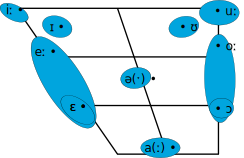
\includegraphics[width=.4\textwidth]{graphics/vowelcharts/pembrokeshire-stressed-penultima}}
  \subtop[Unstressed syllables before a consonant]{\includegraphics[width=.4\textwidth]{graphics/vowelcharts/pembrokeshire-unstressed-preconsonantal}}
  \subtop[Unstressed syllables before a vowel]{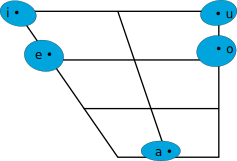
\includegraphics[width=.4\textwidth]{graphics/vowelcharts/pembrokeshire-unstressed-hiatus}}
  \subtop[Unstressed syllables word-finally]{\includegraphics[width=.4\textwidth]{graphics/vowelcharts/pembrokeshire-unstressed-word-final}}
  \caption{Vowels in Pembrokeshire Welsh}
  \label{fig:pw-vowels}
\end{figure}

\subsection{Diphthongs}
\label{sec:diphthongs-2}

Pembrokeshire Welsh has a relatively rich inventory of diphthongs, especially if we include sequences that look like rising diphthongs, such as \ipa{[we]}. However, it appears that the true phonological diphthongs (understood as tautosyllabic non\hyp onset vowels) are falling. I consider these first and then turn to the more problematic cases.

\subsubsection{Falling diphthongs}
\label{sec:falling-diphthongs}

In falling diphthongs, the non-syllabic element is either \ipa{[i]} or \ipa{[u]}. The quality of the nuclear element is for the most part identical to that of the corresponding monophthong, with the exception of \ipa{[ei]} and \ipa{[ou]}, where the nuclear vowel is higher than the monophthong (thus \phonint{e̝i~o̝u}), presumably due to some coarticulation from the following glide. All the diphthongs are shown in \cref{ex:pw-diphthongs}. As I discuss in \cref{sec:structure-diphthongs}, I analyse the offglides as featurally identical to high vowels, so in phonological transcription I will use the symbols \ipa{[i]} and \ipa{[u]} for the offglides.

\ex.\label{ex:pw-diphthongs}\a.\a.\fwe{ˈwein}{ˈwe̝i̯n}{gwaun}{moor}
\b.\fwe{ˈbraiχ}{brai̯x}{braich}{arm}
\b.\fwe{ˈtroi}{ˈtrɔi̯}{troi}{turn}
\b.\fwe{ˈhuir}{ˈhʊi̯r}{hwyr}{late}
\z.\b.\a.\fwe{ˈɬiu}{ˈɬɪu̯}{lliw}{colour}
\b.\fwe{ˈteu}{ˈtɛu̯}{tew}{fat}
\b.\fwe{ˈbraud}{ˈbrau̯d}{brawd}{brother}
\b.\fwe{ˈmour}{ˈmo̝u̯r}{mawr}{big}
\b.\fwe{ˈtəuiɬ}{ˈtəwˑiɬ}{tywyll}{dark}

As noted by \citet[p.~15]{awbery86:_pembr_welsh}, almost all diphthongs are \enquote{paired}, in the sense that both sets of diphthongs contain one diphthong with a high nucleus, one with a low nucleus, and two with mid nuclei (with the one in the same backness category as the glide being low-mid and the one in the same backness category being mid-high). Only \ipa{[əu]} is isolated in this respect, since there is no *\ipa{[əi]} in this dialect.\footnote{It seems that Standard Welsh \ipa{[əi]} (or \ipa{[əɨ]} in dialects which have \ipa{[ɨ]}; see \citealt[p.~727]{gyg}) often corresponds to Pembrokshire \phonint{e̝ĭ}.}

Phonetically, according to \citet[p.~16]{awbery86:_pembr_welsh}, the diphthongs are realized identically across most stress-related contexts: \blockquote{[t]he second element of the diphthong is [\ldots] predictably short in most contexts. This is true of [stressed] monosyllables, and of unstressed antepenultimates and finals.} In stressed penultimate syllables, however, the glide is said to be lengthened.

\ex.\a.\twp{ˈke̝jˑnɔɡ}{ceiniog}{penny}
\b.\twp{ˈe̝jˑra}{eira}{snow}
\b.\twp{ˈtəwˑiɬ}{tywyll}{dark}

\subsubsection{Gliding as phonetic readjustment}
\label{sec:gliding-as-phonetic}

At first blush, Pembrokeshire Welsh also possesses a rich inventory of what looks like rising diphthongs. However, in all of these cases the form with the glide is said to be in variation with one with a full vowel. One example of this variable gliding is found with unstressed high vowels before stressed vowels of penultimate syllables:

\ex.\label{ex:diwrnod-diawl}\a.\a.\twe{[duˈarnod]}{diwrnod}{day}
\b.\mbp{ˈdwarnod}
\z.\b.\a.\twe{[diˈaːvol]}{diawl}{devil}
\b.\mbp{ˈdjaːvol}

I suggest that in this case the variation is probably best described as phonetic. Given that high vowels are pronounced as tense allophones \phonint{i} and \phonint{u} before other vowels (as discussed in \cref{sec:unstressed-syllables}), the difference between a relatively short (in unstressed position) high vowel \phonint{i} (with a relatively narrow constriction) and a glide \phonint{j} is very small and possibly quantitative rather than qualitative. In other words, a short \phonint{i} or \phonint{u}, perhaps lacking a stable formant structure because of short duration, is easy to perceive as a glide rather than the nucleus of a syllable. Given that the conditions for the variation are not well described, I will take the conservative option and interpret it as non\hyp phonological: I will treat the forms in \cref{ex:diwrnod-diawl} as having surface\hyp phonological representations with three syllables: \ipa{[.di.ˈaː.vol.]}, \ipa{[.du.ˈar.nod.]}.

Once we accept that phonological surface vowels can be perceived as glides when they stand next to another, phonetically longer, vowel, we are in a position to understand the more puzzling type of gliding, which involves stressed vowels.

When a stressed high vowel stands in hiatus with a non-high vowel, there is an optional realization where the vowel is glided and the length is realized on the unstressed vowel. This happens irrespective of the presence of a morpheme boundary between the vowels: in \cref{bues}, the two vowels are separated by a morpheme boundary, whereas \cref{diod} is monomorphemic.

\ex.\a.\label{diod}\a.\twe{[ˈdiːod]}{diod}{drink}
\b.\mbp{ˈdjoːd}
\z.\b.\label{bues}\a.\twe{[ˈbiːes]}{bues}{(I) was}
\b.\mbp{ˈbjeːs}

Most surprisingly, this can lead to the creation of what is transcribed as a long vowel before a consonant sequence: a structure that is otherwise all but impossible in the language (\cref{sec:non-final-position}).\footnote{In addition, this type of lengthening may be out of line with the pattern of length specific to that particular morpheme (\cref{sec:contr-vowel-length}): \phonint{ˈfjoːl} `bowl' (\emph{ffiol}) despite plural \ipa{[ˈfjole]} (not *\ipa{[fjoːle]}).} In addition, the gliding seems to create complex onsets, which, as I discuss in \cref{sec:analysis-9}, are dispreferred in Pembrokeshire Welsh.

\ex.\a.\a.\twe{[ˈtuːarχ]}{tywarch}{peat}
\b.\mbp{ˈtwaːrχ}
\z.\b.\a.\twe{[ˈdiːolχ]}{diolch}{thanks}
\b.\mbp{ˈdjoːlχ}

I suggest that also in these cases there is no phonological alternation involved. The difference is due to a trade-off in phonetic length caused by the specifics of the phonetic implementation of stress. I propose that the surface\hyp phonological representation of a form like \phonint{ˈdjoːlχ} is still \ipa{[ˈdiːolχ]}; the transcription with an initial glide simply reflects the fact that the final unstressed vowel is phonetically longer than the stressed vowel. Given the phonetic similarity between tense high vowels \phonint{i~u}, which are the normal realization of stressed vowels in this position, and glides \phonint{w~j}, it is not at all surprising that a vowel can be pronounced and/or perceived as more glide-like in the neighbourhood of a phonetically longer vowel.

There are several reasons for the lengthening of the unstressed vowel. First, all relevant sequences consist of a high vowel followed by a non-high one (sequences of two high vowels are discussed in \cref{sec:flip-flop-altern}), and the greater inherent length of the latter might be a factor here. A second, probably more important, consideration involves the phonetic realization of stress and prominence. I discuss the distribution of length and its relationship to stress, as well as the phonological status of the relevant facts, in greater detail later (\cref{sec:real-stress-polysyll,sec:pros-prom-as}), but the basic idea is that, as shown by numerous investigations \citep{thomas67:_welsh,rhys84:_inton,williams85:_pitch_welsh,williams-eurospeech,williams99:_welsh,ball01:_welsh_phonet}, in certain prosodic contexts a phonologically unstressed final-syllable vowel can be phonetically long, to the point of being longer than the stressed vowel. Given this relationship, we could expect the phonetically shorter vowel of the penultimate syllable to be perceived as more of a glide.

The rôle of phonetic duration as a cue to prosodic structure in this pattern is underscored by the existence of examples such as the following:

\ex.\a.\label{ex:clywais}\a.\twe{[ˈkluːes]}{clywes}{(I) heard}
\b.\mbp{ˈklweːs}
\z.\b.\label{ex:clyw-clywed}\a.\twe{[ˈkləued]}{clywed}{to hear}
\b.\twe{[ˈkliu]}{clyw}{hearing}

The existence of forms such as those in \cref{ex:clyw-clywed} establishes beyond reasonable doubt that the underlying form of the stem \textsc{hear} is \ipa{/kləu/}; the expected 1st person past tense form of \cref{ex:clywais} is thus \ipa{[ˈkləues]} (\cf above \ipa{[ˈbiːes]} for the suffix). Similarly,  \ipa{[ˈtuːarχ]} `peat' is (at least historically) derived from \ipa{[ˈtəuarχ]}.\footnote{\citet[p.~154]{awbery86:_pembr_welsh} indeed records \ipa{[ˈtowarχ]} for `peat' in western varieties (where surface \ipa{[ə]} is dispreferred).} As mentioned in \cref{sec:falling-diphthongs}, the \enquote{glide} in such forms is pronounced long, and the phonetic distance between a \enquote{long glide} and a tense high vowel is not great. Once again, the timing in the recorded form such as \phonint{ˈklweːs} would appear to be an artefact of the phonetic distribution of length rather than of a phonological process. First, the supposed \enquote{glide} becomes more perceptually prominent than the stressed vowel (\phonint{ˈkl\textsuperscript{ə}uˑes} for phonological \ipa{[ˈkləues]}), but the glide itself can in turn be \enquote{hijacked} by the phonetic length of the following vowel, giving \phonint{ˈklweːs}.\footnote{The importance of the final syllable seems to be confirmed by \posscite{awbery86:_pembr_welsh} remark that \ipa{[i]} may be optionally pronounced as \phonint{ji} in a final unstressed syllable: \phonint{ˈmɛnjiw} or \phonint{mɛniw} for \ipa{[ˈmeniw]} `woman', \phonint{hɛðjiw} or \phonint{ˈheːðjiw} for \ipa{[ˈheːðiw]} `today'. It appears likely that the \phonint{ji} is also a product of phonetic lengthening, and the explicit association with the final unstressed syllable is suggestive.} Such \enquote{loss} of stressed vowels with retention of final ones has been extensively commented upon in the literature \citep{jones49:_moder_welsh,watkins76:_cyfnew_gymraeg,bosch96:_promin}, although usually treated from a diachronic standpoint or as a phonological process rather than as a matter of synchronic phonetic variation.

Further evidence for the phonetic nature of this \enquote{gliding} process is found in cases where the \enquote{glided} vowel is in fact mid. \citet{awbery86:_pembr_welsh} records variation of the following type:

\ex.\a.\a.\twe{[ˈdeːaɬ]}{deall}{understand}
\b.\mbp{ˈdiːaɬ}
\b.\mbp{ˈdjaːɬ}
\z.\b.\a.\twe{[ˈhiːol]}{heol}{farmyard}
\b.\mbp{ˈhjoːl}
\b.\mbp{ˈhewl}

There is no productive phonological process of raising that would explain the variation between \ipa{[e]} and \ipa{[i]} in these forms. However, if what is intended as a mid vowel is phonetically short enough compared to its neighbouring vocoid, it can be perceived as a glide (a front one in \phonint{ˈdjaːɬ} or, conversely, a back one in \phonint{hewl}). No appeal to variable, exception-creating phonology is needed: we only have to accept that the phonology\endash phonetics interface (or perhaps the postlexical phonology) in Pembrokeshire Welsh can severely disrupt the relative length (or in any case the perceptual prominence) of stressed and unstressed vowels.\footnote{Of course it is entirely possible that at least some speakers have begun to phonologize these patterns; however, discovering these patterns would require closely targeted empirical study, which I must leave for the future.}


\subsection{Consonants}
\label{sec:consonants}

The phonetic inventory of Pembrokeshire Welsh is shown in \cref{tab:pw-consonans}. Variants given with slashes indicate contextual allophony. I use the devoicing diacritic (as in \eg \phonint{ð̥}) to indicate that the relevant segment does not have consistent vocal fold vibration but retains other characteristics participating in the expression of the laryngeal contrast (\eg length, formant movements etc.).

\begin{table}[htp]
  \centering
\adjustbox{width=\textwidth}{  \begin{tabular}{l*{10}{>{\ipafont}l>{\ipafont}r}}
\toprule
Manner & \multicolumn{2}{c}{Bilabial} & \multicolumn{2}{c}{Labiodental} & \multicolumn{2}{c}{Dental} & \multicolumn{2}{c}{Alveolar} & \multicolumn{2}{c}{Postalveolar} & \multicolumn{2}{c}{Palatal} & \multicolumn{2}{c}{Velar}  & \multicolumn{2}{c}{Uvular} & \multicolumn{2}{c}{Glottal} \\
\midrule
Stops        & pʰ/p & b/b̥ &   &   &   &   & tʰ/t   & d/d̥   &     &      &   &  & kʰ/k & ɡ/ɡ̊ &   &  &    \\
Affricates   &   &   &   &   &   &   &     &     & (ʧʰ) & (dʒ/d̥ʒ̊) &   &  &   &   &   &  &    \\
Fricatives   &   &   & f & v/v̥ & θ & ð/ð̥ & s ɬ & (z/z̥) & ʃ   &      &   &  &   &   & χ &  & h  \\
Nasals       & m &   &   &   &   &   & n   &     &     &      &   &  & ŋ &   &   &  &    \\
Laterals     &   &   &   &   &   &   & l   &     &     &      &   &  &   &   &   &  &    \\
Rhotics      &   &   &   &   &   &   & r/r̥/ɾ/ɹ   &     &     &      &   &  &   &   &   &  &    \\
Approximants & w &   &   &   &   &   &     &     &     &      & j &  &   &   &   &  &    \\
\bottomrule
  \end{tabular}}
  \caption{Pembrokeshire Welsh consonants: the phonetic inventory}
  \label{tab:pw-consonans}
\end{table}

The contrast between \enquote{voiced} and \enquote{voiceless} stops is in reality one between variably voiced and aspirated stops: according to \citet[p.~13]{awbery86:_pembr_welsh}, \textquote{[v]oiceless stops are heavily aspirated in word-initial position, less so elsewhere}, while \textquote{[v]oiced stops and fricatives are fully voiced between vowels, partially voiced in other contexts.} This accords well both with non-instrumental descriptions of other Welsh varieties (\cf for instance \citealt{thomas61:_ffonem_dyffr_wysg,jones,brycheiniog}) and phonetic studies \citep{ball-phon,ball01:_welsh_phonet}.\footnote{A notable feature of the realization of laryngeal contrast in other Welsh varieties (and also in contact varieties of English, cf.\ \citealt{walters03:_celtic_englis}) is the existence of strong postaspiration in word-final and syllable-final position, which are more commonly associated with lack of release and phenomena such as glottalization in other languages. Note, however, that \citet{morris10:_phonet_north_wales} finds that some (Northern) Welsh speakers use variable (\ie \enquote{non\hyp normative} in \citeauthor{helgason}'s \citeyear{helgason} terms) preaspiration for coda stops.} As in many other languages making use of long-lag VOT stops, the laryngeal contrast is neutralized following the fricatives \ipa{[s]}, where stops are voiceless and unaspirated; see below \cref{sec:laryng-assim} for more discussion. The aspiration of stops manifests itself in partial devoicing of following sonorants:

\ex.\a.\twp{ˈpr̥ɛn}{pren}{tree}
\b.\twp{ˈpl̥\kern-1pt ant}{plant}{children}


The laryngeal contrast in fricatives in Welsh dialects is normally one of voicing (rather than VOT); however, as discussed \eg by \citet{ball01:_welsh_phonet}, \enquote{voiced} fricatives can in fact be partially devoiced in a manner similar to stops, although other cues such as duration remain. Since voiced fricatives are relatively rare in non\hyp voicing contexts (\eg word\hyp initially and word\hyp finally, see \cref{sec:phonotactics-1}), a full picture will have to emerge from targeted experimental study.

The rhotic \ipa{[r]} is normally a voiced tap or flap; word-initially, it may be devoiced, but the voiced and voiceless variants are said to be in free variation. Thus, Pembrokeshire Welsh lacks the contrast between \ipa{[r̥]} and \ipa{[r]}, which in other dialects is marginal word-initially but quite robust in non-initial position (however, \ipa{[rh]} sequences are apparently possible: see \cref{sec:story-ipah}).

\ex.\a.\twp{ˈr̥iːχ}{rhych}{furrow}
\b.\mbp{ˈriːχ}

Following alveolar stops, \ipa{[r]} is said to be realized as a fricative \phonint{ɹ}, as in \phonint{ˈdɹuːs} `door' (\emph{drws}).

The segment \ipa{[ŋ]} is found not only word-finally and before velar stops, but also word-medially before a vowel, as in \cref{ex:ng-pw}. It is not found word-initially.

\ex.\label{ex:ng-pw}\a.\twe{[ˈɬɔŋe]}{llongau}{ships}
\b.\twe{[kɪˈvɪŋi]}{cyfyngu}{confine}

The segments \ipa{[ʧ]}, \ipa{[dʒ]}, and \ipa{[z]} are only found in English borrowings, and I exclude them from further consideration here (round brackets in \cref{tab:pw-consonans}).

The inventory I will use in surface\hyp phonological transcriptions is given in \cref{tab:pw-consonants-phonological}. \begin{table}[tbp]
  \centering
\adjustbox{width=\textwidth}{\begin{tabular}{l*{10}{>{\ipafont}l>{\ipafont}r}}
\toprule
Manner & \multicolumn{2}{c}{Bilabial} & \multicolumn{2}{c}{Labiodental} & \multicolumn{2}{c}{Dental} & \multicolumn{2}{c}{Alveolar} & \multicolumn{2}{c}{Postalveolar} & \multicolumn{2}{c}{Palatal} & \multicolumn{2}{c}{Velar}  & \multicolumn{2}{c}{Uvular} & \multicolumn{2}{c}{Glottal} \\
\midrule
Stops        & p & b &   &   &   &   & t   & d   &     &      &   &  & k & ɡ &   &  &    \\
Affricates   &   &   &   &   &   &   &     &     & ʧ & dʒ &   &  &   &   &   &  &    \\
Fricatives   &   &   & f & v & θ & ð & s ɬ & z & ʃ   &      &   &  &   &   & χ &  & h  \\
Nasals       & m &   &   &   &   &   & n   &     &     &      &   &  & ŋ &   &   &  &    \\
Laterals     &   &   &   &   &   &   & l   &     &     &      &   &  &   &   &   &  &    \\
Rhotics      &   &   &   &   &   &   & r/r̥   &     &     &      &   &  &   &   &   &  &    \\
Approximants & w &   &   &   &   &   &     &     &     &      & j &  &   &   &   &  &    \\
\bottomrule
  \end{tabular}}
  \caption{Pembrokeshire Welsh consonants: the phonological inventory}
  \label{tab:pw-consonants-phonological}
\end{table} It is mostly isomorphic with the actual phonological representation, barring a few adaptations to the phonetic reality. The mapping between the surface\hyp phonological transcription used below and phonetics is made explicit in \cref{tab:transcription-pw}. \begin{table}[tbp]
  \centering
  \begin{tabular}{*{2}{>{\ipafont}l}p{.6\textwidth}}
    \toprule
    Phonology & Phonetics & Comments \\
    \midrule
    {[p t k]} & \phonint{p(ʰ) t(ʰ) k(ʰ)} & Aspirated in onsets, unaspirated voiceless (possibly short\hyp lag VOT) following other obstruents. See \cref{sec:laryng-assim} for motivation of the choice of \ipa{[p~t~k]} for the latter context \\
    {[b d ɡ]} & \phonint{b/b̥ d/d̥ ɡ/ɡ̊} & Consistently voiced in intersonorant context, less so elsewhere \\
    {[f θ χ s ʃ ɬ]} & \phonint{f θ χ s ʃ ɬ} & Voiceless, short\hyp lag VOT, relatively long with little contextual allophony \\
    {[v ð]} & \phonint{v/v̥ ð/ð̥}  & Consistently voiced in intersonorant context, less so elsewhere \\
    {[h]} & \phonint{h/ɦ/$\emptyset$} & Described as voiceless when word\hyp initial, sometimes deleted; presumably may be voiced in intersonorant contexts\\
    {[m n ŋ l]} & \phonint{m n ŋ l} & No significant contextual allophony described \\
    {[r/r̥]} & \phonint{r/r̥} & I write \ipa{[r̥]} word\hyp initially and \ipa{[r]} elsewhere despite the lack of phonological distinction to leave the transcription realistic \\
    {[u/w i/j]} & \phonint{w j} & I write \ipa{[u~i]} for monophthongs and off\hyp glides in diphthongs (\ie\ \ipa{[i~u]} that are tautosyllabic with a preceding vowel, even if the high vowel also forms an onset in the following syllable) and \ipa{[w~j]} for \enquote{pure} onsets\\
    \bottomrule
  \end{tabular}
  \caption{Transcription for Pembrokeshire Welsh}
  \label{tab:transcription-pw}
\end{table} In the remainder of this chapter, I will use the simplified transcription of \cref{tab:transcription-pw} for surface\hyp phonological representations, occasionally giving the phonetic forms for clarity.


\section{Prosodic structure and stress}
\label{sec:pros-struct-stress}

In this section I describe the word-level prosodic structure of Pembrokeshire Welsh, deferring discussion of syllable-related matters until \cref{sec:phonotactics-1}.

\subsection{Regular stress}
\label{sec:regular-stress}

As is normal in Welsh dialects otherwise, stress in Pembrokeshire Welsh falls within a two-syllable window at the right edge of the word. The normal situation is penultimate stress, irrespective of the \enquote{size} of the final syllable:

\ex.Final open syllable
\a.Penultimate open syllable
\a.\twe{[ˈboːre]}{bore}{morning}
\b.\twe{[ˈtɔri]}{torri}{to cut}
\z.\b.Penultimate closed syllable
\a.\twe{[ˈkadno]}{cadno}{fox}
\b.\twe{[ˈkɔpsi]}{copsi}{top of corn stack}

\ex.Final closed syllable
\a.Single final consonant
\a.\twe{[ˈskaːdan]}{sgadan}{herring}
\b.\twe{[ˈkrɪvder]}{cryfder}{strength}
\z.\b.Multiple final consonants
\a.\twe{[ˈmənwent]}{mynwent}{cemetery}
\b.\twe{[ˈaskurn]}{asgwrn}{bone}

\ex.Longer forms
\a.\twe{[kʊˈmʊsklid]}{cymysglyd}{muddled}
\b.\twe{[eˈboːles]}{eboles}{filly}
\b.\twe{[karˈθɛni]}{carthenni}{quilts}
\b.\twe{[posiˈbɪlrʊið]}{posibilrwydd}{possibility}
\b.\twe{[kineiˈaːvi]}{cynaeafu}{to harvest}
\b.\twe{[aniˈveiljed]}{anifeiliaid}{animals}

The stress all but never falls further from the right edge than the penultimate syllable, leading to alternations inside paradigms (see \cref{fn:exceptional-stress} below for a brief discussion of exceptions):

\ex.\label{ex:stress-movement}\a.\a.\twe{[ˈeːɡɪn]}{egin}{sprout}
\b.\twe{[ɛˈɡiːno]}{egino}{to sprout}
\z.\b.\a.\twe{[ˈɡɔːvɪn]}{gofyn}{ask}n
\b.\twe{[ɡɔˈvɪnoð]}{gofynnodd}{(s)he asked}

\subsection{Final stress}
\label{sec:final-stress}

In certain exceptional cases stress may fall on the final syllable. These are as follows.

\begin{itemize*}
\item English borrowings
\ex.\a.[]\twe{[sɪˈmɛnt]}{siment}{cement}\par
\item Lexical exceptions
\ex.\a.\twe{[maŋˈɡiː]}{mam-gu}{grandmother}
\b.\twe{[ɪwχˈbɛn]}{uwchben}{above}\par
\item Stems with prefixes (here exemplified by \emph{ail-} `re-')
\ex.\a.\twe{[ailˈhɔi]}{ailhau}{reseed}
\b.\twe{[ailˈneid]}{ailwneud}{redo}*\par
\item Diphthongs derived from vowel sequences straddling a morpheme boundary (synæresis):
\ex.\a.\twe{[ˈkəvle]}{cyfle}{chance}
\b.\twe{[kəvˈleis]}{cyfleus}{convenient}\par
Note that normally final-syllable diphthongs do not attract stress:
\ex.\a.[]\twe{[ˈdamwain]}{damwain}{accident}\par
\item Certain suffixes such as the verbalizing suffix \ipa{[ai]}:
\ex.\a.\twe{[ˈjaːχ]}{iach}{healthy}
\b.\twe{[jaˈχaːd]}{iachâd}{cure}
\b.\twe{[jaˈχai]}{iacháu}{to cure}\par
\end{itemize*}

\subsection{The realization of stress in polysyllables}
\label{sec:real-stress-polysyll}

I assume that the phonetic realization of stress in Pembrokeshire Welsh is not substantially different from that described for other varieties or for the language in general \citep{sommerfelt,jones49:_moder_welsh,pilch57:_lauts,watkins61:_ieith,thomas67:_welsh,rhys84:_inton,williams85:_pitch_welsh,williams99:_welsh,ball01:_welsh_phonet,bosch96:_promin,webb11:_welsh_englis}. Broadly speaking, the stressed (penultimate) syllable demonstrates certain durational properties, to which I return shortly, while final syllables (whether stressed or unstressed), in many prosodic contexts, host a rapid rise in pitch and a concomitant increase in duration \citep[\cfm][]{ohala78:_produc}. These durational and tonal characteristics of final syllables often conspire to give word\hyp final unstressed syllables greater perceptual prominence (at least in the ears of English speakers) than the preceding, stressed, syllable.\footnote{Many of the aspects of this system are also present in the prosodic system of Welsh English, both in the south \citep{walters03:_celtic_englis,walters03:_south_wales_valley_englis} and in the north \citep{webb11:_welsh_englis}.}

Despite this potential for greater salience of the final unstressed syllable, I follow the traditional description in identifying the penultimate syllable as stressed. This is because, as discussed above in \cref{sec:stress-headedness}, I take \enquote{stress} to refer to status as prosodic headship: stressed syllables should be the loci of phonological head\endash dependent asymmetries, and in \cref{sec:foot-intern-struct} I show that this is precisely the case for penultimate syllables in Welsh polysyllabic words.

As noted by \citet{jones67:_welsh,williams85:_pitch_welsh,williams99:_welsh,ball01:_welsh_phonet,webb11:_welsh_englis}, a very important phonetic cue of stress in Welsh is the lengthening of the consonant following a short stressed vowel in a penultimate syllable. It is indeed noted by \citet{awbery86:_pembr_welsh} for Pembrokeshire Welsh as well; she uses a \enquote{half-length} notation. This also covers the lengthening of the glide in a stressed diphthong described above (\cref{sec:diphthongs-2}).

\ex.\label{ex:penult-cons-lengthening}\a.\twp{ˈkarˑeɡ}{carreg}{stone}
\b.\twp{ˈamˑser}{amser}{time}
\b.\twp{ˈejˑra}{eira}{snow}

In \cref{sec:foot-intern-struct}, I analyse this lengthening as moraicity of the postvocalic consonant or glide, and identify the phonological nature of \enquote{stress} as bimoraicity. It would then be not surprising if the main phonetic correlate of stress had to do with highlighting this aspect of the structure of a word, and \citet{williams85:_pitch_welsh} does appear to reach a very similar conclusion: \blockquote[p.~382][.]{The only stress cues seem to be of a relational nature, concerning the relative timing of vowel and consonant, or the temporal arrangement of syllables into feet}

Although I believe this broad picture to be correct, there is an unresolved issue here requiring further study, which concerns the expression of stress in syllables with long vowels. Most previous work has concentrated on stressed syllables with short vowels. Part of the reason is that it is difficult to find minimal pairs with open penultimate syllables. As we saw in \cref{sec:final-stress}, unpredictable stress is rare, and the best chance of finding minimal pairs is connected with prefixes associated with monosyllabic stems, as in \posscite[']{williams85:_pitch_welsh} pair \emph{ymladd} \ipa{[ˈəmlað]} `fight'\,$\sim$\,\emph{ymlâdd} \ipa{[əmˈlaːð]} `tire oneself', and the lexicon of Welsh happens not to provide such forms where the penultimate stressed syllable would have a long vowel. Another aspect skewing the literature towards cases with a short vowel even in open syllables is the concentration on North Welsh: as briefly discussed above in \cref{sec:bryth-quant-syst} and exemplified below in \cref{sec:vowel-length}, in North Welsh \emph{all} stressed vowels in penultimate syllables are short, meaning that the pattern seen in \cref{ex:penult-cons-lengthening} is much more widespread than in South Welsh. The interaction of the hypothesis that it is relative duration within the head syllable that is the main phonetic correlate of stress and the vowel length contrast therefore remains understudied for now. I will return to this issue briefly below in \cref{sec:primacy-length}.

Another issue that would benefit from closer study is the status of the lengthening of the final unstressed syllables as phonetic or phonological. In the discussion of phonetic gliding in \cref{sec:gliding-as-phonetic} I assumed that this lengthening is not phonologized, and I transcribe words such as \ipa{[boːre]} `morning' and \ipa{[ˈkopsi]} `top of corn stack' with short vowels in final syllables rather than *\ipa{[ˈboːreː]} or \ipa{[ˈkopsiː]}. Ultimately, the reason for this is the conservative approach to phonological status I adopt by default: since I know of no phonological evidence that would compel us to include this lengthening in the phonology, and the phenomena that are related to this lengthening (pitch accent placement, phonetic gliding) are commonly described in the literature as \enquote{variable}, it seems safer to assume that it is not indeed phonological. It is of course possible that at least for some speakers this lengthening might have entered the postlexical phonology. Absent an interaction with other phonological processes, such an analysis would, however, at the very least require phonetic evidence for categorical distribution of length, which is not available to me at the moment.

I also discuss this issue below in \cref{sec:pros-prom-as}. In any case, even if the lengthening \emph{is} phonological, it would appear quite clear that it only enters the phonology at the postlexical level; the analysis of Pembrokeshire Welsh foot structure provided in \cref{sec:foot-intern-struct} is only intended to account for the output of the word level, meaning that the (non-)existence of final\hyp syllable lengthening in the postlexical phonology is irrelevant. Given all this, at present I consider it justified to retreat to the conservative position and treat the lengthening as a phonetic phenomenon rather than a categorical operation on prosodic structure.

\subsection{Antepenultimate deletion}
\label{sec:antep-delet}

\citet{awbery86:_pembr_welsh} does not describe any secondary stress for Pembrokeshire Welsh (and in general cites very few forms of at least four syllables). However, there is some evidence for foot structure (or rather lack thereof) in the phenomenon of antepenultimate deletion (\cf also \citealt{jones49:_moder_welsh,watkins76:_cyfnew_gymraeg,hannahs11:_welsh}).

Specifically, a vowel in an antepenultimate syllable (which is by necessity unstressed) that is also word-initial can be deleted, as long as the resulting form is in line with the phonotactic structure of the language:

\ex.\label{ex:pw-antepenult-deletion}\a.\a.\twe{[ˈɛskid]}{esgid}{shoe}
\b.\twe{[ˈskɪdje]}{esgidiau}{shoes}
\z.\b.\a.\twe{[ˈaːdar]}{adar}{birds}
\b.\twe{[ˈdɛːrin]}{aderyn}{bird}
\z.\b.\a.\twe{[ˈardal]}{ardal}{area}
\b.\twe{[arˈdaːloð]}{ardaloedd}{areas}
\b.*\mbi{[ˈrdaːloð]}

However, this phenomenon is not noted for longer forms:

\ex.\a.\twe{[aniˈveiljed]}{anifeiliaid}{animals}
\b.*\mbi{[niˈveiljed]}


\subsection{Consonant phonotactics, syllable structure, and vowel length}
\label{sec:phonotactics-1}

In this section I discuss the restrictions on syllable size and possible segment sequences identified by \citet{awbery86:_pembr_welsh}, as well as some phenomena related to sonority repairs. This will set the scene for the discussion of the central issue of vowel length, which is treated in \cref{sec:vowel-length}.

\subsubsection{Consonant sequences}
\label{sec:consonant-sequences-1}

The restrictions on word-initial and word-final clusters are relatively familiar, though I defer discussion of word-final restrictions until later.

\paragraph{Possible sequences}
\label{sec:possible-sequences}

Word-initially,  possible two-consonant sequences are obstruent\endash obstruent and obstruent\endash sonorant. In the former case, these are only \ipa{[sk~st~sp]} (where the stops are voiceless and unaspirated). As for obstruent\endash sonorant sequences, most combinations of manners are allowed, with the exception of fricatives before nasals:

\ex.\a.\twe{[ˈskaːdan]}{sgadan}{herring}
\b.\twe{[ˈklɪst]}{clust}{ear}
\b.\twe{[ˈkneɪ]}{cneu}{nuts}
\b.\twe{[ˈfrɔŋk]}{ffronc}{part of a pigsty}

\citet{awbery86:_pembr_welsh} does not discuss place restrictions in detail; in general in Welsh, there is a dispreference for coronal\endash coronal initial sequences, especially when the first segment is not a stop: \ipa{[sr]} in particular is impossible (not found in the corpus) and \ipa{[sl]} appears to be found mostly in loanwords, although it is not obvious that they are not nativized: \ipa{[sl]}\hyp initial words are well\hyp represented throughout Wales in \citet{thomas00:_welsh}. Similarly, the gap with \ipa{[sr]} could be just historical (given that historically initial *\emph{sr} changed to \emph{fr} while major sources of loanwords such as English also happen not to have \ipa{[sr]}\hyp initial words).

The standard language also allows the cross\hyp linguistically uncommon \ipa{[tl]} and \ipa{[dl]} as in \emph{tlawd} `poor' and \emph{tlws} `pretty': the latter word is unknown to Pembrokeshire informants for \citet{thomas00:_welsh}, and the former does have initial \ipa{[tl]} in the region (although initial \ipa{[kl]} is common in both of these words in other areas).

Three-consonant clusters word-initially are limited to two types. By far the most common is \ipa{[s]}\endash stop\endash sonorant (in principle \ipa{[r]} is most common as the final element):

\ex.\a.\twe{[ˈskraːveɬ]}{scrafell}{scraper}
\b.\twe{[ˈstrɔːdir]}{strodur}{cart saddle}

Another type is relatively unusual: in the sequences \ipa{[ɡwl]} and \ipa{[ɡwr]} the \ipa{[w]}, contrary to expectations (see below \cref{sec:analysis-9}), remains non\hyp syllabic, even though the alternative forms with a vowel are in principle unobjectionable from a phonotactic perspective.

\ex.\a.\label{ex:gwlan-gwrug}\a.\twe{[ˈɡwlaːn]}{gwlan}{wool}
\b.\twe{[ˈɡwriːɡ]}{gwrug}{heather}
\z.\b.\a.*\mbi{[ˈɡuːlan]}
\b.*\mbi{[ˈɡuːriɡ]}

As discussed below in \cref{sec:analysis-9}, the behaviour of \ipa{[ɡw]} sequences in Pembrokeshire Welsh is special in other aspects too. However, I leave a full analysis of forms such as those in \cref{ex:gwlan-gwrug} for further work, since it is not entirely clear to me how \ipa{[ɡwl]} and \ipa{[ɡwr]} sequences are realized (for instance, it would be interesting to know to what extent the labialization gesture overlaps with the following sonorant).

The set of word-medial consonant sequences includes both sequences that are allowed word-initially and a number of others that are best treated as being broken up by a syllable boundary. These latter include sequences which consist of licit codas followed by single onsets, including sonorant\endash obstruent and sonorant\endash sonorant sequences which are impossible word-initially, as seen in \cref{ex:pw-medial-seqs}.

\ex.\label{ex:pw-medial-seqs}\a.\twe{[ˈɡʊmpas]}{o gwmpas}{around}
\b.\twe{[ˈkɛrðɛd]}{cerdded}{to walk}
\b.\twe{[ˈdaχre]}{dechrau}{begin}
\b.\twe{[ˈamlʊɡ]}{amlwg}{obvious}
\b.\twe{[ˈhɛdvan]}{hedfan}{to fly}

Word-medial sequences of three consonants can, for the most part, be analysed as sequences of a licit coda and a licit complex onset; \citet[p.~109]{awbery86:_pembr_welsh} lists some additional restrictions (for instance, only liquids are allowed as third elements in such sequences), but it is not clear to what extent these are principled. Examples are given in \ref{ex:pw-complex-seqs}.

\ex.\label{ex:pw-complex-seqs}\a.\twe{[ˈəsprid]}{ysbryd}{ghost}
\b.\twe{[ˈkɪndron]}{cynrhon}{maggots}
\b.\twe{[ˈmɔχtra]}{mochdra}{filth}

There are some alternations which appear to enforce the above generalization, in that an expected three\hyp consonant sequence that cannot be parsed as consisting of a simple coda and a licit branching onset is simplified (for the second vowel of \cref{ex:dwfn}, see below \cref{sec:rising-sonority}):

\ex.\a.\label{ex:dwfn}\twe{[ˈduːvun]}{dwfn}{deep}
\b.\twe{[ˈdʊnder]}{dyfnder}{depth}
\b.*\mbi{[ˈdʊvnder]}

However, there are a few examples that cannot be explained in this way.

\ex.\a.\label{ex:ieuanc}\a.\twe{[ˈiːvaŋk]}{ifanc}{young}
\b.\label{ex:ieuenctid}\twe{[ˈjɛŋktid]}{ieuenctid}{youth}
\z.\b.\label{ex:pw-parsley}\a.[]\twe{[ˈparsli]}{}{parsley}

Example \ref{ex:pw-parsley} is clearly a borrowing (and recall that \ipa{[sl]} appears to be allowed even if rare in the native lexicon). In \ref{ex:ieuenctid} the offending sequence is broken up by a morpheme boundary at least historically, though given the non-transparent relationship between the forms in \ref{ex:ieuanc} it cannot be taken for granted that \ref{ex:ieuenctid} is synchronically analysable as a complex word.

Finally, if the glides in diphthongs are treated as consonants, there is at least one example of a tri\hyp consonantal sequence involving a glide as the first element and not interpretable as containing an allowed complex onset:

\ex.\a.\twe{[ˈneiɬti]}{neilltu}{apart}
\b.\twe{[neiɬˈtiːol]}{neilltuol}{special}\footnote{The actual form as recorded by \citet{awbery86:_pembr_welsh} is \phonint{neiɬˈtjoːl}, but see \cref{sec:gliding-as-phonetic}.}

\paragraph{Distributional restrictions}
\label{sec:distr-restr}

There are two important restrictions on consonant sequences that are sometimes enforced by alternations.

First, nasals preceding a stop are almost always homorganic with that stop:

\ex.\a.\twe{[ˈpɪmp]}{pump}{five}
\b.\twe{[ˈmɛntiɡ]}{benthyg}{lend}
\b.\twe{[ˈwɪŋki]}{gwenci}{weasel}

This appears to be enforced in alternations, although given the paucity of stop\hyp initial suffixes the examples mostly come from compounding, raising morphological questions (note also the irregular stress in \cref{ex:mam-gu}).

\ex.\a.\a.\twe{[ˈɬiːn]}{Llun}{Monday}
\b.\twe{[ˈɬɪŋɡwin]}{Llungwyn}{Whit Monday}
\z.\b.\a.\twe{[ˈmam]}{mam}{mother}
\b.\label{ex:mam-gu}\twe{[maŋˈɡiː]}{mamgu}{grandmother}

The exceptions are said to be \enquote{very few}, but are found:\footnote{There are many more examples in the corpus, such as \emph{damcaniaeth} `theory', \emph{canpunt} `hundred pounds', \emph{rhanbarth} `region', although it is not known how these are pronounced in the dialect}

\ex.\a.\twe{[ˈamkan]}{amcan}{idea}
\b.\twe{[ˈprɪŋder]}{prinder}{scarcity}\footnote{Given that the root for `scarce' is undoubtedly \ipa{/prin/} in the dialect (\ipa{[ˈprɪn]} `scarce', \ipa{[ˈprɪnaχ]} `scarcer'), the form written \ipa{[ˈprɪŋder]} might represent the over-analysed transcription of a phonetic \phonint{ˈprɪɪ̃der}, where a surface-phonological \ipa{[n]} manifests itself simply as nasalization but is interpreted as a velar nasal \citep[\cfm][]{trigo88}.}

Fricatives do not enforce this requirement (no examples for the non-coronal fricatives \ipa{[f]} and \ipa{[v]}):

\ex.\a.\twe{[ˈhamðen]}{hamdden}{leisure}
\b.\twe{[ˈpʊmθeɡ]}{pymtheg}{fifteen}

Heterorganic sonorant sequences are also allowed:

\ex.\a.\twe{[ˈamluɡ]}{amlwg}{obvious}
\b.\twe{[ˈkʊmni]}{cwmni}{company}

Another restriction concerns laryngeal features: according to \posscite{awbery86:_pembr_welsh} formulation, clusters of two obstruents always agree in voicing. This is largely true in terms of static distribution:

\ex.\a.Voiced obstruent sequences
\a.\twe{[ˈɡʊðɡe]}{gyddfau}{necks}
\b.\twe{[əsˈtɛðvod]}{eisteddfod}{Welsh cultural festival}
\z.\b.Voiceless obstruent sequences
\a.\twe{[ˈkɔpsi]}{copsi}{top of corn stack}
\b.\twe{[ˈpɪstiɬ]}{pistill}{spring}

However, disharmonic sequences of two fricatives appear to be possible: \ipa{[ˈseiθved]} `seventh' (\emph{seithfed}) \ipa{[ˈʊiθved]} `eighth' (\emph{wythfed}) are recorded for all relevant locations in \citet[\emph{sub vocibus}]{thomas00:_welsh}.\footnote{Such sequences are relatively rare in Welsh vocabulary, but lexicographical sources for other dialects seem to confirm that there is no assimilation in these cases, \eg in Nantgarw \citep{thomas93:_tafod_nantg}: \ipa{[aˈrosva]} `sheep fold' (\emph{arhosfa}), \ipa{[ɡorˈfʊisva]} `resting place' (\emph{gorffwysfa}).}

Alternations enforcing this restriction are discussed in \cref{sec:laryng-assim}.

\subsubsection{Word-final phonotactics}
\label{sec:word-final-phon}

There are two aspects of word-final phonotactics that merit discussion here: relaxed restrictions on syllable size and sonority-related repairs.

\paragraph{Syllable size}
\label{sec:syllable-size}

As discussed in \cref{sec:possible-sequences}, most consonant sequences in Pembrokeshire Welsh can be analysed as being broken up by a syllable boundary after the first consonant, meaning that the coda of the syllable is almost always simple. This restriction is relaxed in word-final position, though the possible sequences are all of non-rising sonority (if sonority is defined according to standard assumptions).

\ex.\label{ex:complex-codas}\a.\twe{[ˈɡarð]}{gardd}{garden}
\b.\twe{[ˈklɪst]}{clust}{ear}
\b.\twe{[ˈɡwaɬt]}{gwallt}{hair}
\b.\twe{[ˈdarn]}{darn}{piece}

Such \enquote{complex codas} are also possible in polysyllabic forms, where they are not immediately preceded by a stressed vowel:

\ex.\a.\twe{[ˈfeːnest]}{ffenestr}{window}
\b.\twe{[ˈmənwent]}{mynwent}{cemetery}
\b.\twe{[ˈaskurn]}{asgwrn}{bone}

\citet[pp.~87--94]{wmffre03:_languag_wales} describes the simplification of final consonant sequences in polysyllabic forms as fairly widespread in his Ceredigion material. It would appear that the Pembrokeshire dialects are more conservative in this regard (for instance, they preserve the final sequence in \emph{asgwrn}, which \citeauthor{wmffre03:_languag_wales} \cite*{wmffre03:_languag_wales} singles out as prone to reduction). However, isolated examples of such \enquote{optional} simplification are also found in Pembrokeshire, apparently with alternations (for the \alternation{[u]}{[ə]} alternation, see below \cref{sec:vowel-mutation}):

\ex.\a.\a.\twe{[ˈsaːdurn]}{Sadwrn}{Saturday}
\b.\mbi{[ˈsaːdun]}
\z.\b.\a.[]\twe{[saˈdərne]}{Sadyrnau}{Saturdays}*

\citet{awbery86:_pembr_welsh} does not describe the precise nature of this variation, so I ignore the possibility of this simplification below.

In addition, a word-final consonant sequence may also be preceded by the glide element of a diphthong:\footnote{The forms appear to contain diphthongs rather than bisyllabic sequences with hiatus. If the latter were the case, we would expect the first vowel to be long, \cf bisyllabic \ipa{[ˈdeːaɬ]} `understand'.}

\ex.\a.\twe{[ˈmaint]}{maint}{size}
\b.\twe{[ˈbeirð]}{beirdd}{poets}*

\paragraph{Rising sonority}
\label{sec:rising-sonority}

Final consonant sequences of rising sonority (or, to be more precise, sequences consisting of an obstruent and a sonorant) are impossible in Pembrokeshire Welsh. Such sequences are found morpheme-finally, but when such morphemes are found word-finally, the offending sequence can be repaired in several ways. \citep{welshphonotactics,awbery86:_pembr_welsh,hannahs09:_welsh}. In Pembrokeshire Welsh, the attested repairs are epenthesis, deletion, and gliding, distributed as follows.

\subparagraph{Epenthesis}
\label{sec:epenthesis}

In the most common case, a vowel is epenthesized between the two final consonants. In terms of (phonological) quality, it is always a copy of the closest vocalic segment to the left, \ie of the stressed monophthong or of the glide part of a diphthong:\footnote{That the alternation represents epenthesis and not vowel deletion is confirmed by the existence of non-alternating vowels, as in \ipa{[ˈmuːdul]}\,$\sim$\,\ipa{[muˈduːle]} `haycock (sg.\,$\sim$\,pl.)'; the form *\ipa{[ˈmʊdle]} is phonotactically acceptable.}

\ex.\a.\a.\twe{[ˈɬɛster]}{llestr}{dish}
\b.\twe{[ˈɬɛstri]}{llestri}{dishes}
\z.\b.\a.\twe{[ˈsoudul]}{sawdl}{heel}
\b.\twe{[ˈsoudle]}{sawdlau}{heels}

The alternation seems to be driven by sonority rather than the identity of the consonants as an obstruent or a sonorant, since epenthesis also applies in all-sonorant sequences:

\ex.\a.\twe{[ˈamal]}{aml}{often}
\b.\twe{[ˈamlaχ]}{amlach}{more often}

However, there are occasional instances (apparently lexically determined) where a similar phenomenon applies in a context that cannot be described in terms of rising sonority:

\ex.\a.\a.\twe{[ˈheːlem]}{helm}{corn stack}
\b.\twe{[ˈhɛlmi]}{helmi}{corn stacks}
\z.\b.\label{ex:pw-gwddf}\a.\twe{[ˈɡuːðuɡ]}{gwddf}{neck}
\b.\twe{[ˈɡʊðɡe]}{gyddfau}{necks}

It appears difficult to extract any generalizations as to what besides rising sonority motivates the epenthesis. No other examples are recorded by \citet{awbery86:_pembr_welsh}. In the literary language, both \ipa{[ðɡ]} and \ipa{[lm]} are allowed, although rare in this position for historical reasons (but \cf \emph{ffilm} `film', \emph{balm} `balm', \emph{salm} `psalm'). For the similar sequence \ipa{[rm]}, \citet[\emph{sub voce}]{thomas00:_welsh} records \ipa{[ˈstoːrom]} for \emph{storm} `storm' but \ipa{[ˈfarm]} for \emph{fferm} `farm'. The latter could be a borrowing, although its short vowel contrasts with a long one in the clearly non\hyp nativized \ipa{[ˈɡaːrd]} `(fire) guard'. \citet[§4.13]{schumacher11:_mittel_fruhn} notes that in Middle Welsh epenthesis into the sequences \ipa{[lv]}, \ipa{[rv]}, \ipa{[lm]}, \ipa{[rm]} and \ipa{[ðv]} (the latter being historically present in words such as \ipa{[ˈɡuːðuɡ]}) was regular: Middle Welsh \emph{palyf} `palm', \emph{furyf} `form'. However, it seems than not all modern dialects retain this: Nantgarw \ipa{[ˈpalv]} `paw' \citep[\emph{sub voce}]{thomas93:_tafod_nantg}, Pembrokeshire \ipa{[ˈfirv]} `form' \citep[p.~71]{awbery86:_pembr_welsh}.

As discussed by \citet{hannahs09:_welsh}, despite the fact that the vowel is a copy of the preceding vocoid, it is apparently not an intrusive vowel \citep{levin87:_between,hall-intrusion} similar to that found in Scottish Gaelic, which has been analysed, at least for some dialects, as being an extension of the vocalic gesture \citep{hind-epenthesis,bosch-dejong,hall-intrusion} rather than the result of a phonological operation such as copying \citep{clements-barra,smith-gaelic,nevins10:_local}. In particular, as seen in examples such as \ref{ex:pw-gwddf}, the epenthetic vowel in Pembrokeshire Welsh is visible for the purpose of prosodic structure, since it behaves in line with the restrictions on the distribution of long vowels operative in the language otherwise (see \cref{sec:vowel-length} for details). I will therefore assume that the two vowels are indeed nuclei of two different syllables.

\subparagraph{Deletion}
\label{sec:deletion}

When the potential form with epenthesis would normally be parsed with three vocalic nuclei, epenthesis is blocked and deletion is deployed instead:

\ex.\label{ex:pw-sonority-driven-deletion}\a.\a.\twe{[feˈnɛstri]}{ffenestri}{windows}
\b.\twe{[ˈfeːnest]}{ffenestr}{window}
\b.*\mbi{[ˈfeːnestr]}
\b.*\mbi{[feˈnɛster]}
\z.\b.\a.\twe{[aˈnadli]}{anadlu}{breathe}
\b.\twe{[ˈaːnal]}{anadl}{breath}

As \cref{ex:pw-sonority-driven-deletion} shows, either the final sonorant or the obstruent preceding it may undergo deletion. According to \citet{awbery86:_pembr_welsh}, there is no clear pattern that would predict which process applies in each particular case, although \citet[ch.~22]{wmffre03:_languag_wales} claims that the sequence \ipa{[dl]} prefers deletion of the stop and other sequences normally prefer sonorant deletion; see also \citet{russell84:_welsh,schrijver95:_studies_britis_celtic,thomas95:_un_fryth}.

\subparagraph{The case of [v]}
\label{sec:case-ipav}

Finally, the behaviour of sequences starting with \ipa{[v]} is less predictable. In some cases, they undergo regular epenethesis.

\ex.\a.\a.\twe{[ˈtreːven]}{trefn}{order}
\b.\twe{[ˈtrɛvni]}{trefnu}{arrange}
\z.\b.\a.\twe{[ˈoːvon]}{ofn}{fear}
\b.\twe{[ˈɔvni]}{ofni}{to fear}

In other cases, the \ipa{[v]} is (variably) realized as a glide \ipa{[w]}; the resulting sequences are, according to \citet[p.~95]{awbery86:_pembr_welsh}, indistinguishable from \ipa{[ʊ]}-final diphthongs (though this has not been verified experimentally):

\ex.\label{ex:cefn-sofl-ysgafn}\a.\twe{[ˈkɛun]}{cefn}{back}
\b.\twe{[ˈsoul]}{sofl}{stubble}
\b.\twe{[ˈəskaun]}{ysgafn}{light}

However, this gliding is probably not a strategy for repairing sonority violations: in these particular forms the gliding of the \ipa{[v]} applies also in non-final syllables, where it cannot be motivated by sonority.

\ex.\a.\twe{[ˈkɛune]}{cefnau}{backs}
\b.\twe{[əsˈkaunaχ]}{ysgafnach}{lighter}

It would seem that the forms in \cref{ex:cefn-sofl-ysgafn} simply represent new underlying forms with diphthongs rather than \ipa{[v]}\endash sonorant sequences. That this is a lexical phenomenon is confirmed by the coexistence of different underlying representations (as in \ipa{[ˈkowru]} or \ipa{[ˈkəvru]} for \emph{cyfrwy} `saddle'), and by the fact that there are differences among dialects as to which lexical items allow which variants, indicating that the new forms are spreading by lexical diffusion. I will therefore ignore this behaviour of \ipa{[v]} in the formal account.

Remarkably, \citet{awbery86:_pembr_welsh} claims that in polysyllabic forms with \ipa{[v]} (\ie for those speakers who have not changed the representation of the lexical item to contain a diphthong) the entire sequence is retained:\footnote{This might be a peculiarity of the sequence \ipa{[vn]}: as noted by \citet{hannahs09:_welsh}, this sequence is more regularly allowed word-finally in Northern Welsh \citep[\egm][\emph{s.\,vv.\@} \emph{cefn}, \emph{cafn}, \emph{ofn}, \emph{dwfn}]{thomas00:_welsh}, as are other \ipa{[v]}\endash sonorant sequences (\emph{gafr}, \emph{llyfr}, \emph{llyfn}). The special status of \ipa{[v]} with respect to rising\hyp sonority consonant sequences in Brythonic languages is also discussed below in \cref{sec:asid-prov-leon}.}

\ex.\a.\twe{[ˈəskavn]}{ysgafn}{light}
\b.*\mbi{[ˈəskav]}
\b.*\mbi{[ˈəskan]}

\subsubsection{Restrictions on single consonants}
\label{sec:restr-single-cons}

Most single consonants may appear in most positions in the word. However, there are some restrictions that are also enforced by alternations.

\paragraph{Initial consonants}
\label{sec:initial-consonants}

Some consonants never appear in initial position. These are \ipa{[ð]} (where \ipa{[v]} is acceptable), \ipa{[θ]}, \ipa{[χ]}, and \ipa{[ŋ]}. Note than all of these are possible in the context of mutation: \ipa{[ð]} is the soft mutation of \ipa{[d]}, \ipa{[θ]} and \ipa{[χ]} are the spirant mutation correspondents of \ipa{[t]} and \ipa{[k]}, and \ipa{[ŋ]} is the nasal mutation of \ipa{[ɡ]}.

At first blush, one could assume that the lack of these segments word\hyp initially is a historical accident. Specifically, voiced fricatives only go back to postvocalic stops, meaning they are almost never found in initial position outside mutation contexts: the few instances found in Modern Welsh are either the result of context-free mutation, as in \emph{fel} `as, how', Middle Welsh \emph{mal}, \emph{ual}, or the dropping of an initial vowel, as in \emph{felly} `so', Middle Welsh \emph{yuelly} \citep{wg-mj,simonevans}. Similarly, \ipa{[θ]} and \ipa{[χ]} go back to geminates (or arise in positions following other segments, \eg liquids, being by necessity non\hyp initial) and \ipa{[ŋ]} could only appear before \ipa{[ɡ]}. All these structures were impossible in initial position at earlier stages of the language.

However, as discussed by \citet{awbery86:_pembr_welsh}, these restrictions are also enforced by the phonology, in that antepenultimate deletion (\cref{sec:antep-delet}) is disallowed if the resulting form were to begin with one of these consonants:

\ex.\a.\twe{[ˈiːχel]}{uchel}{high}
\b.\twe{[iˈχeːlaχ]}{uwch}{higher}
\b.*\mbi{[ˈχeːlaχ]}

\paragraph{Final consonants}
\label{sec:final-consonants}

Most consonants can be found in final position (though \ipa{[h]} is apparently excluded). However, the voiced fricatives \ipa{[v]} and \ipa{[ð]} have a less stable status, in that in certain lexical items they are deleted in this position:

\ex.\a.\a.\twe{[ˈklau]}{clawdd}{hedge}
\b.\twe{[ˈklɔðje]}{cloddiau}{hedges}
\z.\b.\a.\twe{[ˈtreː]}{tref}{town}
\b.\twe{[ˈtreːvið]}{trefoedd}{towns}

However, in other lexical items they remain stable:

\ex.\a.\a.\twe{[ˈkriːv]}{cryf}{strong}
\b.\twe{[ˈkriːvaχ]}{cryfach}{stronger}
\z.\b.\a.\twe{[ˈbeːð]}{bedd}{grave}
\b.\twe{[ˈbeːðe]}{beddau}{graves}

The distinction seems to be purely lexical: \blockquote[\citealt{awbery86:_pembr_welsh}, p.~100]{The choice of which items drop the \ipa{[v]} and \ipa{[ð]} and which keep them is very consistent throughout the area. There are no indications of geographical variation, with one district taking the trend further than another}. This is consistent with data from \citet{thomas00:_welsh}, where deletion of final \ipa{[ð]} and \ipa{[v]} is clearly restricted lexically: it completely fails in some words and varies geographically in others. For instance, \ipa{[ˈpriːð]} `soil', \ipa{[ˈkriːð]} `cobbler', and \ipa{[ˈprauv]} `test' appear with final fricatives throughout Wales,\footnote{Where the word is known: for instance, knowledge of the word \ipa{[ˈprauv]} was denied by the Pencaer informants.} while \emph{cryf} `strong' appears as \ipa{[krɨː]} in most of North Wales but \ipa{[ˈkriːv]} in the south. Conversely, \emph{clawdd} is realized as \ipa{[ˈklauð]} in most localities, with \ipa{[ˈklau]} clearly a south-western form.

Both laryngeal classes of final stops, on the other hand, are found word-finally:

\ex.\a.\a.\twe{[ˈhaːd]}{had}{seed}
\b.\twe{[ˈkrʊt]}{crwt}{boy}
\z.\b.\a.\twe{[ˈsɛld]}{seld}{dresser}
\b.\twe{[ˈsʊɬt]}{swllt}{shilling}
\z.\b.\a.\twe{[ˈkɪndruɡ]}{cynddrwg}{as bad}
\b.\twe{[ˈɬɔk]}{lloc}{sheepfold}

\paragraph{Restrictions on \ipa{/h/}}
\label{sec:restrictions-ih}

The segment \ipa{[h]} falls under a number of additional restrictions. Most importantly, it only appears initially and immediately before a stressed vowel (in which latter case it may only be preceded by a vowel or a nasal). This leads to alternations such as the following:\footnote{Unfortunately \citet{awbery86:_pembr_welsh} gives no examples of a similar alternation following a vowel. In the standard language, the alternation is found not only following nasals but also with \ipa{[r̥]}, as in \emph{arhosaf} `(I) will wait'\,$\sim$\,\emph{aros} `to wait', but \ipa{[r̥]} is absent from the inventory in Pembrokeshire Welsh, although \ipa{[rh]} sequences are recorded in \citet{thomas00:_welsh}; see further \cref{sec:story-ipah}. Following vowels, the standard language mostly prescribes retention of \ipa{[h]} in all contexts, as in \emph{cyhoeddi} `announce'\,$\sim$\,\emph{cyhoedd} `public' (but \emph{ar goedd} `common knowledge'), though a few items follow the restriction on \ipa{[h]}: \emph{ehangu} `widen'\,$\sim$\,\emph{eang} `wide' \citep[§II.53]{gyg}.}

\ex.\a.\a.\twe{[kənˈheia]}{cynhaeaf}{harvest}
\b.\twe{[kəneiˈaːvi]}{cynaeafu}{to harvest}
\z.\b.\a.\twe{[brenˈhiːnes]}{brenhines}{queen}
\b.\twe{[ˈbrɛnin]}{brenin}{king}

In addition, an onset \ipa{[h]} does not prevent antepenultimate deletion (\cref{sec:antep-delet}), even though technically the resulting sequence would be phonotactically impossible:

\ex.\a.\twe{[ˈhɔsan]}{hosan}{sock}
\b.\twe{[ˈsaːne]}{hosanau}{socks}
\b.*\mbi{[ˈhsaːne]}

In \cref{sec:story-ipah} I offer an analysis of the distribution of \ipa{[h]} as a deletion\dash or rather a selective preservation\dash process, building on work by \citet{hannahs11:_welsh}.

Finally, the segment \ipa{[h]} can in fact be freely deleted from all contexts, though the nature of the variation is not described in detail by \citet{awbery86:_pembr_welsh}:

\ex.\a.\a.\twe{[kənˈheia]}{cynhaeaf}{harvest}
\b.\mbi{[kəˈneia]}
\z.\b.\a.\twe{[ˈheːn]}{hen}{old}
\b.\mbi{[ˈeːn]}

Given the lack of data, I ignore this variability in the analysis that follows.

Phonotactic restrictions on consonants other than \ipa{[h]} are summarized in \cref{tab:pw-phonotactic-restrictions}. The question marks refer to cases where I have not been able to locate a dialect form (although the written language may have some of the relevant sequences; see \cref{sec:data-5} below for more discussion).

\begin{sidewaystable}
  \centering
  \begin{tabular}{>{\ipafont}l*{7}{>{\ipafont}c}}
    \toprule
          &                  & \multicolumn{4}{c}{Adjacent segment} &                                                                               \\
    \cmidrule{3-6}
    Class & Word-initial     & Voiced stop                          & Voiceless stop & Voiced fricative & Voiceless fricative & Word-final          \\
    \midrule
    p t k & \checkmark       & \delmark                             & \checkmark     & ?                & \checkmark          & \checkmark          \\
    b d ɡ & \checkmark       & \delmark                             & \delmark       & \checkmark       & \delmark            & \checkmark          \\
    v ð   & \scm v *ð        & \checkmark                           & ?              & \checkmark       & \checkmark          & \delmark/\checkmark \\
    f θ χ & \scm f *θ *χ     & \delmark                             & \checkmark     & \checkmark       & ?                   & \checkmark          \\
    s ʃ ɬ & \checkmark       & \delmark                             & \checkmark     & ?                & ?                   & \checkmark          \\
    m n ŋ & \scm m \scm n *ŋ & \checkmark                           & \checkmark     & \checkmark       & \checkmark          & \checkmark          \\
    l r   & \checkmark       & \checkmark                           & \checkmark     & \checkmark       & \checkmark          & \checkmark          \\
    \bottomrule
  \end{tabular}
  \caption{Phonotactic restrictions on consonants in Pembrokeshire Welsh}
  \label{tab:pw-phonotactic-restrictions}
\end{sidewaystable}

\subsubsection{Vowel length}
\label{sec:vowel-length}

The issue of the predictability of vowel (or rather monophthong) length is central to the prosody of the Brythonic languages, and Pembrokeshire Welsh is no exception in this regard. In this section I provide a description of the distributional facts, with the analysis to follow below in \cref{sec:foot-intern-struct} in the context of well-defined phonological representations.

As discussed by \citet{welshphonotactics,awbery86:_pembr_welsh}, the length of stressed vowels (whether in penultimate or final syllables) in Welsh is tightly connected to the nature of the consonant following the vowel. The relationship is particularly involved in southern dialects (including Pembrokeshire Welsh), where the vowel length contrast is found in both final and penultimate syllables; in northern dialects, the contrast is always neutralized in stressed penultimate syllables in favour of the short vowel:

\ex.South Welsh
\a.Final stressed syllables (overwhelmingly monosyllables)
\a.\twe{[ˈdiːn]}{dyn}{man}
\b.\twe{[ˈɡwɪn]}{gwyn}{white}
\z.\b.Penultimate stressed syllables
\a.\twe{[ˈaːraɬ]}{arall}{other}
\b.\twe{[ˈkareɡ]}{carreg}{stone}

\ex.\label{ex:northwelsh-vowel-length}North Welsh
\a.Final stressed syllables (overwhelmingly monosyllables)
\a.\twe{[ˈdɨːn]}{dyn}{man}
\b.\twe{[ˈɡwɨn]}{gwyn}{white}
\z.\b.Penultimate stressed syllables
\a.\twe{[ˈaraɬ]}{arall}{other}
\b.\twe{[ˈkaraɡ]}{carreg}{stone}

Since the restrictions on vowel length in stressed penultima and final stressed syllables are rather similar in Pembrokeshire Welsh, in what follows I treat them together. I also give the forms in both phonological and highly detailed phonetic transcription. Vowel quality is irrelevant, with the exception of \ipa{[ə]}, on which see \cref{sec:central-vowel}.

\paragraph{Contrastive vowel length}
\label{sec:contr-vowel-length}

Vowel length is contrastive in stressed syllables before the segments \ipa{[n]}, \ipa{[l]}, and \ipa{[r]}, \ie both long and short vowels are encountered before these consonants, with a lexical distribution. (Recall that I ignore the lengthening of final syllables discussed in \cref{sec:real-stress-polysyll}.)

\ex.Monosyllables
\a.The nasal \ipa{[n]}
\a.\fwe{ˈsuːn}{ˈsuːn}{sŵn}{noise}
\b.\fwe{ˈɡrʊn}{ˈɡrʊn}{grwn}{ridge of ploughland}
\z.\b.The lateral \ipa{[l]}
\a.\fwe{ˈsiːl}{ˈsiːl}{Sul}{Sunday}
\b.\label{ex:pw-wal}\fwe{ˈwal}{ˈwal}{wal}{wall}
\z.\b.The rhotic \ipa{[r]}
\a.\fwe{ˈtiːr}{ˈtʰiːr}{tir}{land}
\b.\fwe{ˈbɪr}{ˈb̥ɪr}{byr}{short}

\ex.Penultima
\a.The nasal \ipa{[n]}
\a.\fwe{ˈkaːnol}{ˈkʰaˑnɔl}{canol}{middle}
\b.\fwe{ˈaner}{ˈanˑɛr}{anner}{heifer}
\z.\b.The lateral \ipa{[l]}
\a.\fwe{ˈkoːla}{ˈkoˑla}{cola}{barley awn}
\b.\fwe{ˈkalon}{ˈkalˑɔn}{calon}{heart}*
\z.\b.The rhotic \ipa{[r]}
\a.\fwe{ˈboːre}{ˈboˑre}{bore}{morning}
\b.\fwe{ˈtɔri}{ˈtɔrˑi}{torri}{to cut}

In all other contexts, vowel length in stressed syllables is predictable.

\paragraph{Predictable vowel length}
\label{sec:pred-vowel-length}

All stressed vowels are long before voiced stops and voiced fricatives:

\ex.\a.\a.\fwe{ˈkriːb}{ˈkr̥iːb̥}{crib}{comb}
\b.\fwe{ˈɬaːð}{ˈɬaːð̥}{lladd}{to kill}
\z.\b.\a.\fwe{ˈmuːdul}{ˈmuˑdʊl}{mwdwl}{haycock}
\b.\fwe{ˈaːvon}{ˈaˑvɔn}{afon}{river}

Stressed vowels are always short before voiceless stops:

\ex.\a.\fwe{ˈkrʊt}{ˈkr̥ʊtʰ}{crwt}{boy}
\b.\fwe{ˈsɔpas}{ˈsɔpʰˑas}{sopas}{cold porridge}

Before voiceless fricatives, there is a difference among contexts. In monosyllables, stressed vowels before all voiceless fricatives are long:\footnote{\citet{awbery86:_pembr_welsh} notes some exceptions with a short vowel, though at least two of these would appear to be clitics: \ipa{[ɔs]} `if', \ipa{[drɔs]} `over', \ipa{[bɪθ]} `ever'.}

\ex.\a.\fwe{ˈr̥aːf}{ˈr̥aːf}{rhaff}{rope}
\b.\fwe{ˈnoːs}{ˈnoːs}{nos}{night}
\b.\fwe{ˈpeːɬ}{ˈpʰeːɬ}{pell}{far}

In penultimate syllables, vowels before \ipa{[f~θ~χ]} are long and vowels before \ipa{[s~ʃ~ɬ]} are short.\footnote{However, \citet[p.~24]{awbery86:_pembr_welsh} notes that length before \ipa{[f~θ~χ]} is not very robust, and that \enquote{in some cases} short vowels are in fact found before these segments, in \enquote{free variation}, as in \phonint{ˈkɛːfil}\,$\sim$\,\phonint{ˈkɛfil}. \citet{awbery86:_pembr_welsh} seems to imply this is a new development which represents a simplification of the pattern (since length before fricatives becomes uniform across the penultimate context). Given the unclear status of this phenomenon, I do not consider it further.}

\ex.\a.\a.\fwe{ˈlasoɡ}{ˈlasˑɔɡ̊}{lasog}{gizzard}
\b.\fwe{ˈdɪɬad}{ˈdɪɬˑad̥}{dillad}{clothes}
\z.\b.\a.\fwe{ˈkɛːfil}{ˈkʰɛˑfɪl}{ceffyl}{horse}
\b.\fwe{ˈiːχel}{ˈiˑχɛl}{uchel}{high}


All vowels are short before the nasals \ipa{[m~ŋ]}:\footnote{\citet{welshphonotactics} notes that long vowels are extremely rare but possible before \ipa{[m]}; however, her example \ipa{[ˈbiːm]} `(I) was' (\emph{bûm}) is doubtful, since this preterite paradigm is usually not found in the dialects; the 1st person singular preterite of `to be' in Pembrokeshire Welsh is \ipa{[ˈbiːes]}. In any case, in this particular form the vowel \ipa{[iː]} actually represents a sequence of two \ipa{[i]}'s straddling a morpheme boundary; the exceptional properties of such structures are considered in \cref{sec:synaresis}, and I assume a similar analysis could be leveraged for \emph{bûm} as well.}

\ex.\a.\a.\fwe{ˈtrʊm}{ˈtɹ̥ʊm}{trwm}{heavy}
\b.\fwe{ˈɬɔŋ}{ˈɬɔŋ}{llong}{ship}
\z.\b.\a.\fwe{ˈɛmin}{ˈɛmˑɪn}{emyn}{hymn}
\b.\fwe{ˈaŋen}{ˈaŋˑɛn}{angen}{need}

Finally,  stressed vowels are short before consonant sequences (though \cf \cref{sec:gliding-as-phonetic}) and long when no consonant follows. Significantly, even sequences that would appear to be reasonable complex onsets also disallow long vowels.

\ex.\a.\a.\fwe{ˈɛbriɬ}{ˈɛbˑriɬ}{Ebrill}{April}
\b.\fwe{ˈtɔrθ}{ˈtɔrθ}{torth}{loaf}
\z.\b.\a.\fwe{ˈdiː}{ˈd̥iː}{du}{black}
\b.\fwe{ˈɬiːen}{ˈɬiˑɛn}{lliain}{cloth}

Previewing the analysis, the overall picture at this stage is as follows: a stressed syllable contains either a long vowel or a short vowel and a single (half-long) consonant. While some consonants (\ipa{[n~l~r]}) can be either long or short (and thus can be preceded by either type of vowel), most others are invariably either short or (half-)long depending on their feature make-up; the only exception is the set of \enquote{strident} (\citeauthor{awbery86:_pembr_welsh}'s term) fricatives \ipa{[s~ʃ~ɬ]}, which are short word-finally but long word-medially. I submit that this behaviour of consonants and vowels represents an \emph{explanandum}, \ie that the gaps are not accidental \citep[following][]{wells79:_final_welsh}.

It must be noted that the relationship between vowel length and (obstruent) voicing may apparently break down in newer English borrowings, although \citet{awbery86:_pembr_welsh} does not discuss them. For now I will ignore them, in particular since the behaviour of such borrowings is not described in detail. While this represents an idealization, I would suggest that it is an allowable one, since the system without borrowings is (was) also clearly possible. I return to this issue in somewhat more detail below in \cref{sec:concl-typol-impl}.


\paragraph{The central vowel}
\label{sec:central-vowel}

The behaviour of the central vowel \ipa{[ə]} for the purposes of length is different from that of the other vowels. As described by \citet[§2.3]{awbery86:_pembr_welsh}, the following conditions regulate its length:

\begin{itemize*}
\item In contexts where other vowels are predictably short, \ipa{[ə]} is always short:
\ex.\a.\twp{kʰəˈvarˑʊi̯ð̥}{cyfarwydd}{familiar}
\b.\twp{ˈəstɪr}{ystyr}{meaning}\par
\item In contexts which allow a length contrast, \ipa{[ə]} is also always short:
\ex.\a.\twp{ˈkʰənˑar}{cynnar}{early}
\b.\twp{ˈkʰərˑað̥}{cyrraedd}{to arrive}\par
\item In contexts where other vowels are predictably long, \ipa{[ə]} is either short or long, with an unpredictable distribution:
\ex.\a.\twp{ˈɬəˑɡad̥}{llygad}{eye}
\b.\twp{ˈɬədˑan}{llydan}{wide}\par
Occasionally a lexical item can allow both variants:
\ex.\a.\twp{ˈr̥əˑvɛl}{rhyfel}{war}
\b.\mbp{ˈr̥əvˑɛl}\par
\item The exception from the above generalization is that \ipa{[ə]} is never found before vowels and as a stressed word-final vowel (where other vowels are long).
\end{itemize*}

The overall generalization is that lengthening of \ipa{[ə]} is avoided, being allowed (as one option) only in contexts where other vowels \emph{must} be long.

\paragraph{Diphthongs}
\label{sec:diphthongs-3}

With respect to vowel length in diphthongs, the nucleus in the diphthong is always short, irrespective of its position in the word. As noted above, the glide element is lengthened if the nucleus is penultimate in the word:

\ex.\a.Monosyllables
\a.\fwe{ˈɬai}{ˈɬai̯}{llai}{less}
\b.\fwe{ˈtɛu}{ˈtʰɛu̯}{tew}{fat}
\z.\b.Penultimate prevocalic
\a.\fwe{ˈɡeia}{ˈɡ̊e̝i̯ˑa}{gaeaf}{winter}
\b.\fwe{ˈtəui}{ˈtʰəu̯ˑi}{tywydd}{weather}
\z.\b.Penultimate preconsonantal
\a.\fwe{ˈeira}{ˈe̝i̯ˑra}{eira}{snow}
\b.\fwe{ˈkaudel}{ˈkʰau̯ˑdɛl}{cawdel}{muddle}


\section{Alternations and analysis}
\label{sec:altern-analys}

In this section I propose a contrastive hierarchy and a set of featural specifications for Pembrokeshire Welsh, and then consider alternations, which, together with distributional patterns discussed in \cref{sec:invent-struct}, provide evidence for this particular featural analysis.

\subsection{Representations}
\label{sec:representations}

The contrastive hierarchy I propose for Pembrokeshire Welsh is shown in \cref{fig:welsh-hierarchy}; see also \cref{tab:pw-vowel-features,tab:welsh-consonants} below for a different presentation. \begin{sidewaysfigure}
  \raggedleft\setlength\level{20mm}
\adjustbox{width=\textheight}{%
\begin{tikzpicture}[hierarchy,level 1/.style={sibling distance=24em}]
\node {\ipa{p b d t k ɡ f v θ ð s ʃ ɬ χ h m n ŋ l r i u e o a ə}}
  child[level 2/.style={sibling distance=10em},level 3/.style={sibling distance=8em},level 4/.style={sibling distance=4em}] {node {C-man[cl] \\ \ipa{p b t d k ɡ}}
    child[narrow] {node {C-pl[lab] \\ \ipa{p b}}
      child {node {C-lar[SG] \\ \ipa{p}}}
      child {node {C-lar \\ \ipa{b}}}}
    child {node {C-pl \\ \ipa{t d k ɡ}}
      child {node {C-pl[cor] \\ \ipa{t d}}
        child {node {C-lar[SG] \\ \ipa{t}}}
        child {node {C-lar \\ \ipa{d}}}}
      child {node {C-pl \\ \ipa{k ɡ}}
        child {node {C-lar[SG] \\ \ipa{k}}}
        child {node {C-lar \\ \ipa{ɡ}}}}}}
  child[level 2/.style={sibling distance=17em}] {node {C-man \\ \ipa{f v θ ð s ʃ ɬ χ h m n ŋ l r i u e o a ə}}
    child[every child/.style={sibling distance=3em}] {node {C-man[LL] \\ \ipa{v ð}}
      child {node {C-pl[lab] \\ \ipa{v}}}
      child {node {C-pl \\ \ipa{ð}}}}
    child {node {C-man \\ \ipa{f θ s ʃ ɬ χ h m n ŋ l r i u e o a ə}}
      child[narrow] {node {V-man[op] \\ \ipa{a e}}
          child {node {V-pl[cor] \\ \ipa{e}}}
          child {node {V-pl \\ \ipa{a}}}}
        child {node {V-man \\ \ipa{f θ s ʃ ɬ χ h m n ŋ l r i u o ə}}
          child[narrow] {node {V-man[cl] \\ \ipa{o ə}}
            child {node {V-pl[cor] \\ \ipa{ə}}}
            child {node {V-man \\ \ipa{o}}}}
        child {node {V-man \\ \ipa{f θ s ʃ ɬ χ h m n ŋ l r i u}}
          child[every child/.style={sibling distance=8em}] {node {C-lar[SG] \\ \ipa{f θ s ʃ ɬ χ h}}
            child[narrow] {node {V-man[cl] \\ \ipa{s ʃ ɬ}}
              child {node {C-pl[cor] \\ \ipa{s ʃ}}
                child {node {V-pl[cor] \\ \ipa{ʃ}}}
                child {node {V-pl \\ \ipa{s}}}}
              child {node {C-pl \\ \ipa{ɬ}}}}
            child[narrow] {node {V-man \\ \ipa{f θ χ h}}
              child {node {C-man[op] \\ \ipa{f θ χ}}
                child {node {C-pl[lab] \\ \ipa{f}}}
                child {node {C-pl \\ \ipa{θ χ}}
                  child {node {C-pl[cor] \\ \ipa{θ}}}
                  child {node {C-pl \\ \ipa{χ}}}}}
              child {node {C-man \\ \ipa{h}}}}}
          child[every child/.style={sibling distance=9em}] {node {C-lar \\ \ipa{m n ŋ l r i u}}
            child[narrow] {node {C-pl[cor] \\ \ipa{n l r}}
              child {node {V-man[op] \\ \ipa{n l}}
                child {node {V-man[cl] \\ \ipa{n}}}
                child {node {V-man \\ \ipa{l}}}}
              child {node {V-man \\ \ipa{r}}}}
            child[every child/.style={sibling distance=6em}] {node {C-pl \\ \ipa{m ŋ i u}}
              child {node {C-pl[lab] \\ \ipa{m}}}
              child[narrow] {node {C-pl \\ \ipa{ŋ i u}}
                child {node {V-pl[cor] \\ \ipa{i}}}
                child[every child/.style={sibling distance=6em}] {node {V-pl \\ \ipa{ŋ u}}
                  child {node {V-pl[lab] \\ \ipa{u}}}
                  child {node[fill-node] {C-pl[dor] \\ \ipa{ŋ}}}}}}}}}}};
\end{tikzpicture}}
\caption{The contrastive hierarchy for Pembrokeshire Welsh}
\label{fig:welsh-hierarchy}
\end{sidewaysfigure} A detailed rationale for these featural representations will be given in the following sections together with a formal analysis; in this section I discuss the features I propose for Pembrokeshire Welsh.

To save space in tableaux, I will use the notation \us{segment} to designate features for which the given segment is the unit segment, or as a shorthand for feature bundles. The shorthands for most features are given in  \cref{tab:pw-shorthands}.

\label{pw-diacritics}I will also use a set of diacritics to designate the addition of features that result in impossible segments. I will use the aspiration symbol \ipa{[ʰ]} to refer to the addition of a \fea{C-laryngeal}{spread glottis} feature to a segment that ordinarily does not bear it: for instance, \ipa{[n]} is \{\fea{C-place}{coronal}, \fea{V-manner}{closed}\}, and the notation \ipa{[nʰ]} will be used for \{\fea{C-place}{coronal}, \fea{V-manner}{closed}, \fea{C-laryngeal}{spread glottis}\}. Similarly, I will use the voicing diacritic to refer to segments that have a bare C-laryngeal node: for instance, if \ipa{[θ]} is \{\fea{C-manner}{open}, \fea{C-place}{coronal}, \fea{C-laryngeal}{spread glottis}\}, then \ipa{[θ̬]} is \{\fea{C-manner}{open}, \fea{C-place}{coronal}, C-laryngeal\}. Finally, the devoicing diacritic will refer to complete deletion of the C-laryngeal specification: \ipa{[θ̥]} is \{\fea{C-manner}{open}, \fea{C-place}{coronal}\}.

\begin{table}[htp]
  \centering
  \begin{tabular}{ll}
    \toprule
    Feature & Shorthand \\
    \midrule
    \fea{C-manner}{closed} & \us{ɡ} \\
    \fea{C-manner}{lowered larynx} & \us{ð} \\
    \fea{C-manner}{open} & None \\
    \fea{C-place}{coronal} & \us{r} \\
    \fea{C-place}{labial} & \us{m} \\
    \fea{C-place}{dorsal} & \us{ŋ} \\
    \fea{C-laryngeal}{spread glottis} & \us{h} \\
    \midrule
    \fea{V-manner}{open} & \us{a} \\
    \fea{V-manner}{closed} & \us{o} \\
    \fea{V-place}{coronal} & \us{i} \\
    \fea{V-place}{labial} & \us{u} \\
    \bottomrule
  \end{tabular}
  \caption{Shorthand notation for features in Pembrokeshire Welsh}
  \label{tab:pw-shorthands}
\end{table}


The set of features I propose for Pembrokeshire Welsh is, for the most part, relatively orthodox: thus, \fea{C-manner}{closed} designates stops, and there is a small but relatively unsurprising set of place features such as \fea{C-place}{labial} and \fea{C-place}{coronal}. However, the representation of laryngeal contrast and manner features requires more comment.

\subsubsection{Laryngeal contrasts}
\label{sec:laryngeal-contrasts}

In this section I discuss the \enquote{special} feature \fea{C-manner}{lowered larynx} used to distinguish \enquote{voiced fricatives}, and the presence of a bare C-laryngeal node in sonorants.

\paragraph{The specification of voiced fricatives}
\label{sec:spec-voic-fric}

As \cref{fig:welsh-hierarchy} shows, I propose that phonetic laryngeal contrast is represented in several different ways in the phonology of this language. Thus, the contrast between different types of stops (\ie \fea{C-place}{closed} segments) is represented using a \fea{C-laryngeal}{spread glottis} feature: \enquote{fortis}, \ie aspirated, stops bear this feature, while \enquote{lenis} (variably voiced) stops have a bare C-laryngeal node. In phonological terms, this means that lenis stops are expected to interact with features residing on the C-laryngeal tier (in practice only \fea{C-laryngeal}{spread glottis}) in phonological processes; this is indeed the case, as I show in \cref{sec:analysis-10}.

On the other hand, the laryngeal contrast between fricatives is represented in a completely different way. I propose a \emph{manner} feature, which I, for convenience, call \fea{C-manner}{lowered larynx} \citep{trigo91:_phary,youssef10:_laryn_buchan_scots}. The key insight here is that despite the phonetic similarity between the laryngeal contrasts which exist between \enquote{fortis} and \enquote{lenis} stops and fricatives, the phonological behaviour of \enquote{lenis} stops is very different from that of \enquote{lenis} fricatives, in that the latter are inert in processes involving the feature \fea{C-lar}{SG}. The best way to formalize this is to assume that the relevant feature simply resides on a different tier. I propose that it is the manner tier.

Treating a laryngeal contrast in terms of manner is far from unprecedented: a connection between laryngeal features (primarily voicing) and related features such as tongue root advancement and/or height has been proposed before \citep{trigo91:_phary,vaux96:_status_atr_featur_geomet,youssef10:_laryn_buchan_scots}. Phonetically, larynx lowering is a strategy for raising the transglottal pressure differential which is required to sustain voicing \citep[\egm][]{riordan80:_laryn_englis,kohler84:_phonet,phon-knowledge}, but since voicing is also tightly bound to the value of F$_{1}$ \citep[\egm][]{kingston08}, it is not surprising that it becomes allied to vowel height and similar features. This pattern can be further phonologized to include interactions between laryngeal features in consonants and [ATR]/[RTR] or vowel height, as in Buchan Scots \citep[\egm][]{kohler84:_phonet,fitzgerald02:_vowel_buchan_scots_englis,paster04:_vowel_buchan_scots,youssef10:_laryn_buchan_scots} or certain Armenian dialects \citep{vaux98:_phonol_armen}. There are no consonant\hyp vowel interactions of this type in Pembrokeshire Welsh (as reflected in the fact that vowel height is expressed on the V\hyp manner rather than C\hyp manner tier), but I suggest nevertheless that voiced fricatives are best treated as bearing a manner feature.\footnote{An alternative approach is treating [lowered larynx] as a V-laryngeal feature, following \citet{youssef10:_laryn_buchan_scots}. The choice between these two is more or less arbitrary in Pembrokeshire Welsh (unlike the Buchan Scots case treated by \citeauthor{youssef10:_laryn_buchan_scots} \cite*{youssef10:_laryn_buchan_scots}, where [lowered larynx] shows the pattern of vowel harmony with possible blocking by intervening consonants characteristic of V-tier features), but the V-laryngeal approach would require relatively complex argumentation to account for the non\hyp interaction of [lowered larynx] segments with \fea{C-laryngeal}{spread glottis}. In the C-manner approach, the inertness follows from the lack of representational relationships between the two classes. This does not preclude the V-laryngeal approach being correct (perhaps for some speakers), but for the moment I am not aware of any evidence that would allow us to distinguish between the two.}

A potential objection to this analysis involves the fact that voicing in lenis fricatives is, according to some descriptions, variable in a manner similar to stops. However, \citet{ball01:_welsh_phonet} report the results of a pilot study with two speakers, of which one shows consistent voicing of lenis fricatives in all positions. In addition, as I discuss below in \cref{sec:does-passive-voicing}, \enquote{variable} voicing is not necessarily inconsistent with the existence of a phonological specification. In any case, more detailed study, in particular with a focus on correlates other than VOT and pure duration, is needed in order to fully explore the phonetic consequences of the present proposal.

\paragraph{The status of C-laryngeal}
\label{sec:status-c-laryngeal}

Another non-trivial element of laryngeal contrast in Pembrokeshire Welsh as proposed in \cref{fig:welsh-hierarchy} is the relatively high rank of the \fea{C-lar}{SG} on the hierarchy. This feature is used to separate the large class of voiceless fricatives from the set \ipa{[m~ŋ~n~l~r~i~u]}. As a result, the latter receive a bare C-laryngeal node, and thus can potentially participate in processes involving features on this tier (\ie \fea{C-lar}{SG}).

I suggest this is a desirable result. As discussed in much previous literature, and below in \cref{sec:nasal-mutation,sec:story-ipah}, all the sonorants (\ipa{[m~ŋ~n~l~r]}) and glides \ipa{[w j]} (which I analyse as featurally identical with \ipa{[u]} and \ipa{i}) can combine with \ipa{[h]} in sequences of the type \ipa{[nh]} or \ipa{[wh]} (which can phonetically be fully or partially devoiced in addition to having positive VOT; \eg\ \citealt{ball-phon}).

\subsubsection{Manner features}
\label{sec:manner-features}

In the system proposed in \cref{fig:welsh-hierarchy}, manner features play a relatively marginal rôle; contrasts expressed in terms of manner are largely catered for by the laryngeal feature \fea{C-lar}{SG}, by the hybrid feature \fea{C-man}{LL}, and by place contrasts, for which sonorants play the rôle of unit segments. C-manner is used to differentiate the large class of stops, as well as the smaller class of \enquote{non-strident} fricatives. As I discuss in the relevant sections below, both of these are coherent classes: stops demonstrate a particular pattern of laryngeal contrast not found in other segments and a subhierarchy of place features that is closely mirrored in the class of \enquote{non\hyp strident} fricatives, with which these stops also alternate.

V-manner features serve to express height contrasts in vowels. They are also used to parcel out the natural class of \enquote{strident} fricatives, which
show a specific type of behaviour in terms of weight, and to express manner contrasts among coronal sonorants.

Perhaps the most important feature of the manner system is the lack of a \enquote{unit segment} for the feature \fea{C-manner}{open}: all \fea{C-man}{op} bear the feature \fea{C-lar}{SG}, in addition to a (possibly empty) C-place node. This featural structure is necessary to derive the correct behaviour of \enquote{non\hyp strident} voiceless fricatives, as discussed especially below in \cref{sec:initial-mutations}. In theoretical terms, it represents an example of computation imposing extrinsic constraints on phonological representation and introducing predictable information (\cref{sec:establ-pred-distr}). Specifically, I assume that the surface system is disrupted by the augmentation constraint \textsc{Have}\hspace{0pt}(\fea{C-lar}{SG})/\fea{C-man}{op}, formulated as in \cref{cons:have-sg-c-man-op}.

\begin{constraint}
  \label{cons:have-sg-c-man-op}
  \consdef{|\pprop{\textsc{Have}(C-lar[SG])/C-man[op]}|:=}{(\prop{output}\wedge\prop{Root}\wedge\langle\downarrow\rangle\pprop{C-man[op]})\to\langle\downarrow\rangle\pprop{C-lar[SG]}}\\
`An output root node that dominates \fea{C-manner}{open} also dominates \fea{C-laryngeal}{spread glottis}'
\end{constraint}


This constraint is ranked sufficiently high to impose epenthesis of \fea{C-lar}{SG} for the \{\fea{C-man}{op}\} candidate provided by the rich base, as shown in \ref{no-unit-segment-for-man-op}; the ranking \dom{\textsc{Max}(\fea{C-man}{op})}{*\fea{C-man}{op}} is established by the fact that \fea{C-man}{op} can surface at all.

\ex.\label{no-unit-segment-for-man-op}No unit segment for \fea{C-man}{op}\\
\wraptbl{\begin{OTtableau}{4}\OTdashes{1,3}\OTsolids{2}
\OTtoprow[\featurebox{\rt,C-man,[op]}{??}]{\textsc{Max}(\fea{C-man}{op}),\textsc{Have}(\us{h})/\fea{C-man}{op},\textsc{Dep}(\us{h}),*\fea{C-man}{op}}
\OTcandrow{\featurebox{\rt,C-man,[op]}{??}}{,*!,,*}
\OTcandrow[\OThand]{\mfeaturebox{\featurestring{\rt,C-man,[op]}\\\featurestring{\rt,C-lar,[SG]}}{χ}}{,,*,*}
\OTcandrow{\featurebox{\rt}{??}}{*!,,,}
\OTcandrow{\featurebox{\rt,C-lar,[SG]}{h}}{*!,,*,}
\end{OTtableau}
}

In \cref{sec:initial-mutations} (pp.~\labelcpageref{sec:aspirate-mutation} \emph{sqq.}) I show how the constraint \textsc{Have}(\fea{C-lar}{SG})/\fea{C-man}{op} can be satisfied using a different mechanism: I argue that the unit segment for this feature is the trigger of aspirate mutation, where the augmentation\hyp driven coalescence of this segment with a following stop produces the mutation effect. This segment can be located in a number of positions on the contrastive hierarchy; I do not show it to reduce clutter.

\subsubsection{Unresolved issues}
\label{sec:unresolved-issues}

In what follows I provide at least a cursory analysis of most alternations discussed by \citet{awbery86:_pembr_welsh} for Pembrokeshire Welsh. In the interest of full disclosure, here I identify patterns for which I do not propose any explicit analysis.

\begin{itemize}
\item Nasal place assimilation. As described in \cref{sec:distr-restr}, although the majority of nasal\hyp stop sequences in the dialect are homorganic, and there are some alternations enforcing this requirement, the generalization is not exceptionless. Given that the phonological status of assimilation\hyp like processes is notoriously difficult to establish, I leave this matter unresolved here. Note that in the system presented in \cref{fig:welsh-hierarchy} both \ipa{[m]} and \ipa{[n]} share C-place features with corresponding stops; although \ipa{[ŋ]} does not (\ipa{[ŋ]} is \fea{C-place}{dorsal} and \ipa{[k~ɡ]} are placeless), it is not at all impossible that the surface \ipa{[ŋ]} found in onsets and the \ipa{[ŋ]} resulting from assimilation are not in fact identical on the surface.
\item Restrictions on initial consonants. Although it seems that restrictions on (at least some) initial consonants are reflected in the phonology (\cref{sec:initial-consonants}), in that an impossible word\hyp initial consonant blocks antepenultimate deletion, the featural system in \cref{fig:welsh-hierarchy} is not set up to reflect these restrictions in terms of natural classes. Although the phonology is certainly able to express them in terms of relatively \emph{ad hoc} constraints, such an account clearly has little explanatory value. In any case, a precise account would require a firmer understanding of which gaps are historical and which are not: for instance, given the historical origins of initial \ipa{[v]} discussed in \cref{sec:initial-consonants}, the fact that initial \ipa{[ð]} is said to be unattested could simply be down to the fact that Middle Welsh did not have sufficiently many words with initial \ipa{[d]} to undergo similar processes.\footnote{Indeed Standard Welsh has at least one (fairly frequent) \ipa{[ð]}\hyp initial word, namely \emph{ddoe} `yesterday' (soft\hyp mutated adverbial \emph{doe}): \citet{thomas00:_welsh} records mostly \ipa{[d]}\hyp initial variants (overwhelmingly \ipa{[ˈduːe]}) in Pembrokeshire. The form \ipa{[ˈðoː]} is found as a variant at one location, but it could be a literary intrusion.} Finally, all the \enquote{impossible} word\hyp initial consonants would appear to be possible as the outcome of mutation. Again, this issued must be left for further research.
\end{itemize}

\subsection{Vocalic alternations}
\label{sec:vocalic-alternations-1}

The representations for the vowels are shown in \cref{tab:pw-vowel-features}; unit segments for each particular feature are shaded for clarity. \begin{table}[tp]
  \centering
  \begin{tabular}{l*{4}{c}}
    \toprule
              & \multicolumn{2}{c}{V-manner} & \multicolumn{2}{c}{V-place}                   \\
    \cmidrule{2-5}
    Vowel     & [closed]                     & [open]        & [coronal]     & [labial]      \\
    \midrule
    \ipa{/i/} &                              &               & \checkmark\gc &               \\
    \ipa{/ə/} & \checkmark                   &               & \checkmark    &               \\
    \ipa{/u/} &                              &               &               & \checkmark\gc \\
    \ipa{/e/} &                              & \checkmark    & \checkmark    &               \\
    \ipa{/o/} & \checkmark\gc                &               &               &               \\
    \ipa{/a/} &                              & \checkmark\gc &               &               \\
    \bottomrule
  \end{tabular}
  \caption{Vocalic representations in Pembrokeshire Welsh}
  \label{tab:pw-vowel-features}
\end{table} All the material in this section should be taken as an extensive argument for this featural proposal; here I will briefly sketch the natural classes, with references to specific discussion elsewhere in this section.

\subsubsection{Natural classes}
\label{sec:natural-classes}

Perhaps that most typologically unusual aspect of this proposal is the treatment of the segment traditionally written as \ipa{[ə]}: while it is normally treated as a \enquote{weak} vowel, up to the point of being featureless \citep{oostendorp00:_phonol}, here it is analysed as having high subsegmental complexity: it has two features rather than one. However, this hypothesis is corroborated by its phonological behaviour: the vowel \ipa{[ə]} alternates with a simpler vowel due to constraints related to feature co\hyp occurrence (\cref{sec:vowel-mutation}), and it is the outcome of a morphologically additive process which I treat in floating\hyp feature terms (\cref{sec:fronting-1}). These alternations also establish its affinity with the segments \ipa{[i]} and \ipa{[o]}, respectively, which is reflected in their shared featural structure: \ipa{[ə]} is essentially the union of the structures of \ipa{[o]} and \ipa{[i]}.

Another class of \enquote{related} vowels is the set \ipa{[a~e~i]}, where is \ipa{[e]} is a more complex vowel containing the features of both simpler ones, as is frequent in privative approaches to vocalic structure such as Element Theory \citep{harris95,harris05:_vowel_reduction,backley11:_elemen_theor}. This is reflected in the existence of processes where docking a feature associated with \ipa{[i]} to the segment \ipa{[a]} results in a surface \ipa{[e]} (\cref{sec:diphth-altern,sec:raising:-data}).

Before treating the alternations in detail, we turn to the question of the relationship between vowel length and vowel quality. \Cref{tab:pw-vowel-mutation} assumes that minor qualitative differences in the realization of short and long vowels (\cref{sec:vowels}) are not phonologically relevant, \ie that the difference between (say) \phonint{i(ː)} and \phonint{ɪ(ː)} is one of quantity, not of (phonological) quality. This is not a trivial assumption, as I discuss in the next section.

\subsubsection{Vowel length and quality}
\label{sec:vowel-length-quality}

The interaction of vowel length and quality in Pembrokeshire Welsh differs somewhat from that found in certain other dialects \citep{watkins61:_ieith,jones}, where the class of \enquote{long} vowels coincides with that of \enquote{tense} ones, at least in stressed syllables. Many analyses of other varieties, especially those embracing a structuralist phonemic framework, assume that only one of these features is contrastive in the language. For instance, \citet[p.~53]{jones} proposes: \blockquote{As regards the place of this length factor in the phonology, it may be treated as a concomitant feature of the qualitative difference that marks the series of vowels termed \enquote{close} above as distinct from those termed \enquote{open} when they occur in stressed positions.} The converse position is defended by \citet{thomas66:_system_welsh}, who says: (p.~122): \blockquote{[t]he only significant difference [\ldots] between the stressed and unstressed systems of the Welsh vowels is the occurrence of length as a phonological unit in the stressed system of all dialects}. Moreover, there is a third logical possibility, namely that both quality and length are in fact phonological, in the sense that phonological computation has access both to the tenseness\fshyp laxness feature and to the length, and then enforce the observed tight fit between the two (\cref{sec:establ-pred-distr}). In this section I defend \posscite[']{thomas66:_system_welsh} position that only length is relevant to the phonology.

\paragraph{The primacy of length}
\label{sec:primacy-length}

Pembrokeshire Welsh is an interesting test case here, because, as discussed in \cref{sec:stressed-penultima,sec:unstressed-syllables}, the qualitative distinctions do not quite match up with quantitative ones. One aspect of the mismatch is the variation found between \enquote{tense} and \enquote{lax} non-low vowels in unstressed position (this is also common for other varieties, as acknowledged by \citealp[p.~54]{jones}). This, in itself, is an argument for treating the length contrast as primary. If vowel quality were phonological, the fact that both \ipa{[e]} and \ipa{[ɛ]} may appear in variation in unstressed syllables would be an \emph{explanandum} for the phonology. Moreover, if the variation does not involve the two categorical variants, but rather is continuous, as seems likely (though I am not aware of relevant instrumental studies), then the phonological analysis involving two discrete categories is highly implausible.

If we assume that \phonint{eː} and \phonint{ɛ(ː)} all in fact represent the same phonological segment (roughly \enquote{front mid vowel}), which can combine with stress and prosodic structure in the phonology, and then can be freely interpreted by the interface, then the variation in unstressed syllables is in fact to be expected. This variation is just another case of broader limits of variation enabled by the lack of phonological contrast \citep{keating88:_under,keating90:_phonet,dyck95:_const,dyck,dresher09}: since speakers know that the phonological vowel \ipa{[e]} can only be short in an unstressed position, they do not attend to the height differences that they otherwise deploy to enhance the length contrast in stressed syllables, and this less tight control leads to greater variability due to mechanical factors.\footnote{Another logical possibility is that speakers may deploy categorical allophony of the sort found by \citet{scobbie09:_dutch,mielke10:_variab_americ_englis}, possibly deploying it for social\hyp indexical purposes \citep{lawson11:_scott_englis}: crucially, such allophony is \emph{not} expected to be driven by purely phonological factors.}

Less speculatively, the question is whether the feature that would potentially enable the distinction between \phonint{ɛː} and \phonint{eː} is in fact phonologically active anywhere in the language. The answer to that seems to be negative: outside the context of the alternation discussed here, the distinction does not appear to be involved in any phonological process.\footnote{Although see below \cref{fn:calediad} on \cpageref{fn:calediad}.}

The conclusion for Pembrokeshire Welsh is that the qualitative distinctions between tense and lax pairs such as \phonint{i~ɪ} are not relevant to the phonology. The phonology only operates on the six vowels listed in \cref{tab:pw-vowel-features}, and \enquote{tenseness} differences are due to the language-specific phonetic implementation component. I will reflect this in surface\hyp phonological transcription from now on.\footnote{Note that the phonological primacy of length does not necessarily means that the relevant vowels should \emph{always} be pronounced as long in actual performance; see the discussion in \cref{sec:real-stress-polysyll}.}

\paragraph{The length of the schwa}
\label{sec:length-schwa}

The central vowel \ipa{[ə]}\footnote{This transcription is rather conventional; for instance, the formant data given by \citet{ball01:_welsh_phonet} a relatively big difference in the quality of this vowel for their two speakers (both of North Welsh dialects, which also have \ipa{[ɨ]} in the inventory). In any case, the vowel is generally a non-labialized central non-high non-low segment, so I retain the traditional typography here.} stands somewhat aloof in the inventory of the dialect.

First, as we have seen, there are a number of restrictions that it does not share with other vowels, such as the impossibility to be the word-final segment (though we shall see below that it is a subcase of a broader restriction) and the impossibility of preceding a vowel. More importantly, there are significant restrictions on the combination of \ipa{[ə]} with length, although phonetically \phonint{əˑ} is not impossible in the dialect.\footnote{Recall that I assume \enquote{half\hyp length} to be the phonetic expression on length in penultimate syllables. Since (long) \ipa{[ə]} is never found in word\hyp final syllables, phonetic \phonint{əː} is excluded.}

There are two problems with interpreting phonetic \phonint{əˑ} as phonological \ipa{[əː]} in parallel with other vowels. First, \ipa{[ə]} is never long in contexts which allow, but do not enforce, vowel length, \ie before the sonorants \ipa{[l~n~r]}, although this is a relatively benign issue: the resulting forms are never phonotactically deviant, there just appears to be a lexical gap. More seriously, if \ipa{[ə]} and \ipa{[əː]} are distinct phonological symbols, then the existence of otherwise unprecedented forms such as \ipa{[ˈɬədan]} `wide', with a short vowel before a voiced stop (\ie not *\ipa{[ˈɬəːdan]}), requires explanation.

I suggest that the length of the schwa is not distinctive in Pembrokeshire Welsh, and that both \phonint{ə} and \phonint{əˑ} represent the phonological symbol \ipa{[ə]}, \ie a short vowel. I assume it is not phonologically long because, first, the schwa is in fact short in most positions and, second, it is excluded precisely from some positions where length is obligatory: it cannot precede a vowel or a word boundary in a stressed syllable. The phonetic difference is appears to be an instance of \enquote{word\hyp specific phonetics} \citep{pierrehumbert02:_word}. As discussed in \cref{sec:role-lexicon}, it is clear that these effects are a challenge to the modular theory \citep{bermudez-otero10:_curren_englis}, although approaches such as \posscite{jackendoff07:_found} parallel architecture do allow the interfaces (where the lengthening would be placed under the present approach) at least some access to the lexicon while retaining overall modularity. Here, I will merely note that this appears to be another instance of a known problem.

The main factor behind the variation is, again, contrast. The speakers' knowledge that \ipa{[ə]} can only ever be phonologically short allows them more latitude in the actual phonetic realization, with the distribution being (apparently) lexical, although it would of course be interesting to know what hides behind \posscite{awbery86:_pembr_welsh} description mentioning \enquote{variation}. For now, I will assume that the vowel \ipa{[ə]} is phonologically short in all surface contexts, and will transcribe it accordingly.

\subsubsection{Vowel mutation}
\label{sec:vowel-mutation}

The label \enquote{vowel mutation} refers to a set of alternations between short high vowels \ipa{[i(ː)]} (\ipa{[ɨ(ː)]} in North Welsh) and \ipa{[u(ː)]} on the hand and \ipa{[ə]} on the other hand (in addition to certain diphthongal alternations), which has attracted considerable theoretical interest \citep{allen75:_vowel_mutat_word_stres_welsh,cartmill76:_welsh_vowel_mutat,thomas84:_north_welsh,awbery86:_pembr_welsh,bosch96:_promin,greenbook,hannahs07:_const_welsh}. In this section I both propose an amended analysis, which combines the insights of \citet{bosch96:_promin}, \citet{greenbook}, and \citet{hannahs07:_const_welsh}, and show how vowel mutation provides evidence for the featural representations in the language.

\paragraph{The data}
\label{sec:data-4}

The \enquote{core} facts in this section concern monophthongs: vowel mutation is defined as the alternation between the high vowels \ipa{[i(ː)]} and \ipa{[u(ː)]} in the final syllable and \ipa{[ə]} in a non-final syllable, which can be exemplified as follows:

\ex.\a.\a.\twe{[ˈkriːv]}{cryf}{strong}
\b.\twe{[ˈkrəvaχ]}{cryfach}{stronger}
\b.\twe{[ˈɡoːvin]}{gofyn}{to ask}
\b.\twe{[ɡoˈvənes]}{gofynnais}{(I) asked}
\z.\b.\a.\twe{[ˈdurn]}{dwrn}{fist}
\b.\twe{[ˈdərni]}{dyrnu}{to thresh}
\b.\twe{[ˈmeːðul]}{meddwl}{to think}
\b.\twe{[meˈðəljəs]}{meddyliais}{(I) thought}

As the examples show, the alternation is clearly tied to word-final position rather than stress, since the \ipa{[ə]} can appear in both stressed and
unstressed syllables. There is also no link to the status of vowel length as contrastive or not: both long and short high vowels may alternate.

When the monophthong in the final syllable is the result of sonority\hyp driven epenthesis \cref{sec:rising-sonority}, \ipa{[u]} remains intact in the non-final syllable:

\ex.\a.\twe{[ˈpudri]}{pydri}{to rot}
\b.\twe{[ˈpuːdur]}{pwdr}{rotten}

However, when the epenthetic vowel is expected to be \ipa{[ə]}, it undergoes the alternation:

\ex.\a.\twe{[ˈɬəvre]}{llyfrau}{books}
\b.\twe{[ˈɬəvir]}{llyfr}{book}
\b.*\mbi{[ˈɬivir]}
\b.*\mbi{[ˈɬəvər]}

A similar alternation is found with the diphthongs \ipa{[iu]} and \ipa{[əu]}. (Recall that there is no \ipa{[əi]} diphthong in the dialect.)

\ex.\a.\twe{[ˈbiu]}{byw}{to live}
\b.\twe{[ˈbəuid]}{bywyd}{life}

Finally, there is a superficially similar alternation between the diphthongs \ipa{[ai]} in a final syllable and \ipa{[ei]} in a non\hyp final syllable.

\ex.\a.\twe{[ˈbraiχ]}{braich}{hand}
\b.\twe{[ˈbreiχe]}{breichiau}{hands}

However, it is not true that all instances of \ipa{[i~u~iu]} in word\hyp final syllables alternate with \ipa{[ə~ə~əu]} respectively:

\ex.\a.\a.\twe{[ˈpliːv]}{pluf}{feathers}
\b.\twe{[ˈpliːvin]}{plufyn}{feather}
\b.\twe{[ˈeːɡin]}{egin}{sprout}
\b.\twe{[eˈɡiːno]}{egino}{to sprout}
\z.\b.\a.\twe{[ˈstuk]}{stwc}{milk pail}
\b.\twe{[ˈstuke]}{stwcau}{milk pails}
\b.\twe{[ˈteilur]}{teilwr}{tailor}
\b.\twe{[teiˈlurja]}{teilwria}{to work as a tailor}
\z.\b.\a.\twe{[ˈɬiu]}{lliw}{colour}
\b.\twe{[ˈɬiuoɡ]}{lliwog}{colourful}

At the same time \ipa{[ə]} is not found in final syllables of content words.\footnote{The vowel \ipa{[ə]} may appear in clitics. Descriptions of Welsh also note that \ipa{[ə]} may appear in final syllables of borrowings as the correspondent to the NURSE vowel, as in \emph{nyrs} \ipa{[ˈnərs]} `nurse', but \citet{awbery86:_pembr_welsh} does not discuss these.}

With regard to the \alternation{[ei]}{[ai]} alternation, all instances of \ipa{[ai]} undergo it (that is, \ipa{[ai]} is impossible in a non\hyp final syllable). However, \ipa{[ei]} is possible in both final and non\hyp final syllables.

\ex.\a.\twe{[ˈwein]}{waun}{moor}
\b.\twe{[ˈeira]}{eira}{snow}

Thus, at least in this case it would seem we would be justified in assuming that the non\hyp alternating \ipa{[ei]} represents underlying \ipa{/ei/}, and alternating \alternation{[ei]}{[ai]} represents underlying \ipa{[ai]} (since there is no non\hyp alternating \ipa{[ai]}). Otherwise, the direction of alternation is not immediately clear. The situation is summed up in \cref{tab:pw-vowel-mutation}, where I assume a non-committal representation for the less clear cases.

\begin{table}[htp]
  \centering
  \begin{tabular}{lcc}
    \toprule
    Unit             & Non-final syllable & Final syllable \\
    \midrule
    \ipa{/i/$_{1}$}  & \ipa{[i]}          & \ipa{[i]}      \\
    \ipa{/i/$_{2}$}  & \ipa{[ə]}          & \ipa{[i]}      \\
    \ipa{/u/$_{1}$}  & \ipa{[u]}          & \ipa{[u]}      \\
    \ipa{/u/$_{2}$}  & \ipa{[ə]}          & \ipa{[u]}      \\
    \ipa{/iu/}$_{1}$ & \ipa{[iu]}         & \ipa{[iu]}     \\
    \ipa{/iu/$_{2}$} & \ipa{[əu]}         & \ipa{[iu]}     \\
    \ipa{/ei/}       & \ipa{[ei]}         & \ipa{[ei]}     \\
    \ipa{/ai/}       & \ipa{[ei]}         & \ipa{[ai]}     \\
    \bottomrule
  \end{tabular}
  \caption{Vowel mutation in Pembrokshire: the standard system}
  \label{tab:pw-vowel-mutation}
\end{table}

In the following sections I present my analysis of the sound pattern, followed by a comparison with other approaches found in the literature, a discussion of the relationship between the present analysis and previous ones, and an account in terms of Optimality Theory.

\paragraph{The \ipa{[i]} $\sim$ \ipa{[ə]} alternation}
\label{sec:status-ipai-sim}

I follow \citet{hannahs07:_const_welsh} in analysing the alternation between \ipa{[ə]} and \ipa{[i]} as the raising of underlying \ipa{/ə/} to \ipa{[i]} in a final syllable.\footnote{As many others concentrating on the alternation, \citet{hannahs07:_const_welsh} focuses on North Welsh, and thus uses \ipa{[ɨ]} for the segment alternating with \ipa{[ə]}. For ease of comparison, I silently rewrite it to \ipa{[i]} when discussing South Welsh.}. Thus, the form \ipa{[ˈkriːv]} `strong', which alternates with \ipa{[ˈkrəvaχ]} `stronger', is derived from underlying \ipa{/krəv/}, while \ipa{[ˈpliːv]} `feathers' (\ipa{[ˈpliːvin]} `feather') is derived from \ipa{/pliv/}. This approach stands in contradistinction to the traditional account, discussed in more detail below in \cref{sec:traditional-analysis}, where the surface \ipa{[ə]} is usually derived from some high vowel.

The main advantage of this approach is that it resolves a number of issues related to the existence of both alternating and non\hyp alternating versions of \ipa{[i]} (the \ipa{/i/}$_{1}$ and \ipa{/i/}$_{2}$ of \cref{tab:pw-vowel-mutation}): non\hyp alternating \ipa{[i]} is \ipa{/i/} and alternating \ipa{[i]} is \ipa{/ə/};  in much of the previous literature this problem was resolved using various diacritic devices, which are not needed in this approach.

A second advantage is that this analysis resolves an issue related to richness of the base. Under standard OT anti\hyp free\hyp ride assumptions  \ipa{[ə]} must be a possible underlying segment in Welsh, since there exist instances of \ipa{[ə]} that never alternate with other vowels, \eg in non-final syllables of polysyllabic roots: \alternation{[ˈməni]}{[məˈnəðe]} `mountain (\alternation{sg.}{pl.})' (\emph{mynydd}, \emph{mynyddoedd}). In this context, it behoves us to ask how an input \ipa{/ə/} is treated in a final syllable, and the raising approach provides a well\hyp founded answer. The lowering approach, on the other hand, would need additional, essentially arbitrary, machinery to account for the behaviour of input \ipa{/ə/} (although \cite{greenbook} argues that it is mapped faithfully, citing borrowings such as \ipa{[ˈnərs]} `nurse'; see below \cref{fn:nurse} for discussion).

There are also some dialectological facts that support the underlying status of \ipa{/ə/}. As noted by \citet{welshphonotactics,awbery86:_pembr_welsh,wmffre03:_languag_wales}, in a large zone covering southern Ceredigion and spilling over into north-east Pembrokeshire, the distribution of \ipa{[ə]} is broader than elsewhere in Wales: it is licensed in (stressed) monosyllables, albeit only as a short vowel. In addition, this region is characterized by an extension of the alternation to items which do not undergo it in other areas, and which must presumably be treated as a change in underlying representation. Thus, in these dialects underlying \ipa{[ə]} is found in more lexical items than elsewhere, and the alternation is governed by somewhat different principles, which are shown in \cref{tab:extended-schwa-system}.

\begin{table}[htp]
  \centering
\adjustbox{width=\textwidth}{\begin{tabular}{l*{6}{c}c}
    \toprule
    & \multicolumn{3}{c}{Standard system} & \multicolumn{3}{c}{Extended system} & \\
    \cmidrule(r){2-4} \cmidrule(l){5-7}
    Gloss & Underlying & Final & Non-final & Underlying & Final & Non-final & Orthography \\
    \midrule
    `lake' & \ipa{/ɬən$_{\mu}$/} & \ipa{[ˈɬin$_{\mu}$]} & \ipa{[ˈɬən$_{\mu}$oð]} & \ipa{/ɬən$_{\mu}$/} & \ipa{[ˈɬən$_{\mu}$]} & \ipa{[ˈɬən$_{\mu}$oð]} & \alternation{\emph{llyn}}{\emph{llynnoedd}} \\
    `long' & \ipa{/hir/} & \ipa{[ˈhiːr]} & \ipa{[ˈhiːraχ]} & \ipa{/hər/} & \ipa{[ˈhiːr]} & \ipa{[ˈhəraχ]} & \alternation{\emph{hir}}{\emph{hirach}} \\
    `lip' & \ipa{/ɡwevis/} & \ipa{[ˈɡweːvis]} & \ipa{[ɡweˈvise]} & \ipa{/ɡwevəs/} & \ipa{[ˈɡweːvis]} & \ipa{[ɡweˈvəse]} & \alternation{\emph{gwefus}}{\emph{gwefusau}} \\
    \bottomrule
  \end{tabular}}
  \caption{The \enquote{extended} system contrasted with the standard}
  \label{tab:extended-schwa-system}
\end{table}

\Cref{tab:extended-schwa-system} shows three lexical items. In the word for `lake', which has an underlying \ipa{/ə/} in both types of varieties, the consonant is distinctively moraic \citep{moren01:_distin}, as shown by the fact that in the standard system the \ipa{[i]} derived by raising is short: \ipa{[ˈɬin]} rather than *\ipa{[ɬiːn]} (see below \cref{sec:distrbiution-morae}). In the extended system, this means that the vowel need not be lengthened, and surfaces faithfully rather than with raising. In the word for `long', the \ipa{[r]} is not moraic, which compels lengthening: thus, even despite the fact that the relevant item has been relexified as containing an underlying \ipa{/ə/}, it has to alternate in the final syllable because the prosody forces it to lengthen: thus \ipa{[ˈhiːr]} rather than *\ipa{[həːr]}.\footnote{This alternation also provides further evidence that long \ipa{[əː]} is not tolerated as a phonological surface element (\cf \cref{sec:length-schwa}).} Finally, the word for `lip' shows that relexification also fails to eliminate alternation in the extended system, presumably because surface \ipa{[ə]} in a final syllable must be licensed by stress: \ipa{[ˈɡweːvis]} rather than *\ipa{[ˈɡweːvəs]}.

In the lowering account, the existence of forms such as \ipa{[ˈɬən]} is utterly unexpected. Once again, this is due to the fact that most approaches simply fail to consider the fate of an underlying \ipa{[ə]}, while surface \ipa{[ə]} is always assumed to derived by lowering. On the other hand, the raising approach provides a straightforward explanation both for the patterns characteristic of the \enquote{extended system} and for its historical origin.

A final argument for treating the alternation as one of raising is structural. The traditional account relying on a rule of \enquote{centralization} for the vowel mutation of \ipa{[i]} assumes that it is the vowel that appears in the final syllable that is underlying. However, as noted by \citet{welshphonotactics}, even traditional descriptions recognize the existence (in other dialects) of the reverse pattern, whereby an unfaithful mapping only happens in the final syllable: the alternation between final\hyp syllable \ipa{[a]} and non\hyp final\hyp syllable \ipa{[e]}, as in the following examples from the dialect of Nantgarw \citep{thomas93:_tafod_nantg}:

\ex.\a.\a.\twe{[ˈsʊpar]}{swper}{supper}
\b.\twe{[sʊˈpeːra]}{swpera}{to have supper}
\z.\b.\a.\twe{[ˈpreːkaθ]}{pregeth}{sermon}
\b.\twe{[prɪˈɡɛθi]}{pregethau}{sermons}

The raising approach to \ipa{[ə]} provides an exact parallel to this pattern.

Very similar argumentation applies to the \alternation{[əu]}{[iu]} alternation: as argued below in \cref{sec:structure-diphthongs}, the elements of diphthongs are no different from vowels in their featural structure, and therefore non\hyp alternating \ipa{[iu]} represents \ipa{/iu/} and alternating \alternation{[əu]}{[iu]} represents underlying \ipa{/əu/}.

In the next section I argue that the unfaithful mapping in the final syllable is driven by a feature co\hyp occurrence constraint sensitive to the presence of a suprasegmental \enquote{prominence} feature.

\paragraph{Prosodic prominence as an abstract feature}
\label{sec:pros-prom-as}

Building on work by \citet{bosch96:_promin}, I suggest that the alternation is driven by the presence of an emergent suprasegmental feature, along the lines discussed in \cref{sec:emerg-supr-feat}. For the sake of the argument, I will call it \enquote{prominence} (written [Prom] and transcribed with an acute accent: \ipa{[é]}). Although this feature plays, at best, a marginal rôle in the lexicon of the language, I suggest that the situation in Welsh represents one of those cases where the a feature is introduced by the computation, rather than by the lexicon, and where its presence can be deduced from the robust phonological patterns that it participates in.

In this sense, its status is related to the status of intonational tones in languages such as English. It is commonly assumed that intonational tones are manipulated by the phonology \citep{pierrehumbert80:_englis,gussenhoven04}; however, unlike languages such as Thai \citep[\egm][]{moren06:_thai}, tones are not stored in lexical representations of English words. These tones are inserted in the (postlexical) phonology, but they are not used by the lexicon; the interaction of tones and segmental structure is also far from unprecedented \citep{hyman74:_univer_tone_rules,hombert78:_conson,jiang-kang99:_tone_optim_theor,tang08,beckerng:_inter_atr_sloven}.

The Welsh \enquote{prominence} feature merely represents a similar phenomenon, albeit introduced at the word level rather than postlexically. This makes sense in the light of the life cycle of phonological processes described in \cref{part:theory}: it represents a remnant of the tone(s) that the postlexical component used to place on stressed syllables before the accent shift (\cref{sec:bryth-quant-syst}), which has now ascended to predictable word\hyp level phonology. This grammaticalization process has not resulted in a pure pitch feature, presumably because of the high variability of the contours that the final syllable could (and still can; \citealp{thomas67:_welsh,pilch75:_advan_welsh,williams85:_pitch_welsh}) bear in different prosodic contexts. What has remained is an abstract, emergent feature (perhaps an example of the \enquote{monster feature} predicted to exist in the substance\hyp free approach), which clearly participates in phonological processes but does not have an invariant phonetic correlate.

As I argued in \cref{sec:contrast-stratal-ot}, this situation does not really violate the Contrastivist Hypothesis. In addition, it is not impossible that it \emph{might} enter the lexicon, because at least some dialects do have words with exceptional stress patterns, such as \ipa{[ˈtelefon]} `phone' \citep{jones}; see also below \cref{fn:nurse}. Admittedly, it is not clear whether it is only the foot head or also the prominence structure that is exceptional here, so this issue must be left for further enquiry.

The nature of this word\hyp final prominence as a feature follows from its behaviour: its presence is reflected by a process which reduces the number of possible contrasts in the relevant position, \ie neutralization. In an OT framework, neutralization is commonly seen as reflecting a markedness\hyp over\hyp faithfulness ranking, and the relevant markedness constraint is easiest to formalize in terms of feature co\hyp occurrence. In this respect, this approach is simpler than other approaches to head\dash stress mismatches (\cref{sec:stress-headedness}), which usually express the mismatch in terms of the different placement of foot heads and grid marks. The ontology of grid marks, however, is not exactly clear, which also leads to significant underdetermination with respect to their possible effects in \emph{segmental} phonology. Treating the prominence as a feature, on the other hand, makes the concrete prediction that its effects will be similar to those of other features, since it will be available to constraints such as feature co\hyp occurrence and featural licensing. We will see in \cref{sec:ot-analysis} that this prediction is borne out in Pembrokeshire Welsh.\footnote{Paul Kiparsky (p.~c.) draws my attention to the fact that the rules of Welsh poetic metre \citep[\egm][]{morris-jones25:_cerdd} treat word-final syllables before a cæsura as pivots for the purposes of alliteration (\cf in particular \citealt{griffen99}), which might be taken as evidence for their status as \emph{metrical} positions. However, even if we ignore the question of the extent to which the highly formalized \emph{cynghanedd} tradition, with roots going back to early medieval, \ie pre\hyp accent\hyp shift (\cref{sec:bryth-quant-syst}), poetic forms, can inform phonological analyses of the modern language, the prosodic analysis is not the only one; \cf the approach of \citet{hammondar:_welsh}, which is based on correspondence domains rather than rhythmic positions.}

Thus, I propose that the phonological computation associates final syllables of prosodic words with the prominence feature.\footnote{Note that this neatly explains the appearance of \ipa{[ə]} in clitics referred to above: not being prosodic words, clitics do not receive the prominence feature, and thus there is no reason for \ipa{[ə]} to raise.} This feature is not placed on the head (\enquote{stressed}) foot of the word, which is the locus of complexity asymmetries (\cref{sec:foot-intern-struct}). This mismatch is exactly parallel to the mismatch between \enquote{stressed} and \enquote{foot heads} in Roman Italian discussed above in \cref{sec:stress-nonhyp-heads}. It is the presence of this feature that motivates the raising of \ipa{[ə]} to \ipa{[i]}. In the next section I turn to another aspect of \enquote{vowel mutation}, namely the alternation between \ipa{[u]} and \ipa{[ə]}, which I argue to have a similar motivation, but an entirely different ontology.

\paragraph{The status of the \ipa{[u]} $\sim$ \ipa{[ə]} alternation}
\label{sec:status-ipau-sim}

If we treat the \alternation{[i]}{[ə]} as derived from an underlying \ipa{/ə/}, then the behaviour of \ipa{[u]} appears to require explanation: \cref{tab:pw-vowel-mutation} shows the existence of both alternating and non\hyp alternating \ipa{[u]}, so it appears that any phonological account requires recourse to some sort of diacritic marking either of an underlying \ipa{[ə]} (negating many of the advantages of the raising account identified in \cref{sec:status-ipai-sim}) or of \ipa{[u]} (again, suboptimal).

To get around this conundrum, I propose, partly following \citet{greenbook}, that the alternation involving \ipa{[ə]} is in fact \emph{not} phonological in Pembrokeshire Welsh; rather, alternating forms are produced via a mechanism involving lexical selection. Specifically, I suggest that the alternation represents an instance of phonologically optimizing allomorph selection \citep{tranel96:_frenc,tranel98:_suppl_ot,kager96,lapointe01:_stem_ot,rubach-booij2001,bermudez-otero06:_morph_spanis,wolf08:_optim_inter}.

I suggest that the phonological system of Pembrokeshire Welsh in general prefers to keep input \ipa{/u/} intact, so if the input presents a form with \ipa{[u]}, it surfaces faithfully: thus, the stem \textsc{rot} has just one form \ipa{/pudr/}, and the computation compels it to surface faithfully in \ipa{[ˈpudri]} `to rot'. At the same time the segment \ipa{[ə]} is generally preferred to \ipa{[u]}, so if a stem allomorph with \ipa{[ə]} is available, it is chosen in order to avoid a surface \ipa{[u]} without violating the faithfulness constraint (since the \ipa{[ə]} is already present in the input). However, since \ipa{[ə]} is prohibited in a final syllable, \ipa{[u]} allomorphs are still chosen in that context. Crucially, this account motivates the \ipa{[ə]} alternations in the final syllable using one and the same constraint, unlike \posscite[']{hannahs07:_const_welsh} approach as discussed in \cref{sec:comp-with-prev}

Moreover, this approach allows us to use the alternation as evidence to motivate the featural structure of vowels. The constraint driving the dispreference for \ipa{[u]}, presumably sensitive to featural structure, is satisfied when the inserted allomorph has the vowel \ipa{[ə]}, which means that \ipa{[ə]} and \ipa{[u]} probably do not share features.

One prediction of this account of the \alternation{[u]}{[ə]} alternation is that it should be unproductive, or very marginally productive. This is somewhat surprising given the relatively large number of items that undergo this alternation (see also \cref{sec:traditional-analysis} for a discussion of the traditional analysis, where it is assumed that \ipa{[u]} \emph{always} alternates with \ipa{[ə]}, and that it is the non\hyp alternating case that requires special explanation).\footnote{Note, however, that \citet{bermúdez-oterong:_spanis} proposes a similar account of the \alternation{\emph{ue}}{\emph{o}} and \alternation{\emph{ie}}{\emph{e}} alternations in Spanish, long considered to be the bread and butter of phonological computation.} Although testing this requires more data than I have access to at the moment, \citet{awbery86:_pembr_welsh} discusses some dialectological evidence which can be construed to support this proposal.

The system of vowel mutation described in \cref{tab:pw-vowel-mutation}, which is more or less that found across South Wales, breaks down in the western part of the Pembrokeshire, largely due to a general dispreference for the vowel \ipa{[ə]}. Where other dialects have \ipa{[ə]}, West Pembrokeshire varieties use \ipa{[i]} or \ipa{[u]}. Most pertinently for our purposes, in morphemes where the \ipa{[ə]} alternates with a high vowel \ipa{[i]} or \ipa{[u]} in the final syllable, the normal pattern is that the same vowel is carried over into non-final syllables, ensuring a faithful mapping throughout.

\ex.Loss of vowel mutation in West Pembrokeshire
\a.\a.\twe{[ˈkriːv]}{cryf}{strong}
\b.\twe{[ˈkriːvaχ]}{cryfach}{stronger}
\z.\b.\a.\twe{[ˈdurn]}{dwrn}{fist}
\b.\twe{[ˈdurni]}{dyrnu}{to thresh}

This is best explained in terms of a restructuring of underlying representations, where morphemes containing \ipa{[ə]} are relexified with \ipa{[i]}, while morphemes containing \ipa{[u]} lose competing allomorphs with underlying \ipa{[ə]}. Some traces of the vowel\hyp mutation pattern are preserved in West Pembrokeshire, with the expected outcome (\ipa{[i]} instead of \ipa{[ə]}).

\ex.\a.\a.\twe{[ˈɬuŋk]}{llwnc}{throat}
\b.\twe{[ˈɬiŋki]}{llyncu}{to swallow}
\z.\b.\a.\twe{[ˈtur]}{twr}{crowd}
\b.\twe{[ˈtiri]}{tyrru}{to crowd}

\citet{awbery86:_pembr_welsh} states that this alternating pattern is clearly recessive, which is to be expected if the alternating rule is driven by opaque, not fully phonological mechanisms. This hypothesis clearly requires further study.\footnote{For instance, the hypothesis would be clearly confirmed if there were cases where the exceptional stem allomorphy is morphosyntactically constrained, \ie where it does not cross major category boundaries (\cf \citeauthor{bermúdez-oterong:_spanis} \cite*{bermúdez-oterong:_spanis}): for instance, if the verbal stem of \textsc{crowd} were exceptional \ipa{/tir/} with the noun stem simultaneously demonstrating regular phonology (\eg plural \ipa{[ˈture]}). Unfortunately there are no examples of such part\hyp of\hyp speech mismatches given by \citet{awbery86:_pembr_welsh} (but neither are there examples where a nominal and verbal derivative from the same root are given simultaneously).}

\paragraph{The diphthongal alternation}
\label{sec:diphth-altern}

Finally, it is not possible to analyse the alternation \alternation{[ei]}{[ai]} in parallel with the \alternation{[i]}{[ə]}, by assuming an underlying \ipa{/ei/} mapping to \ipa{[ai]} in a final syllable, since non-alternating \ipa{[ei]} also exists. This pattern is somewhat parallel to the \alternation{[u]}{[ə]} alternation, as an across\hyp the\hyp board alternation blocked in word-final syllables. Unlike the mutation of \ipa{[u]}, however, the \alternation{[ei]}{[ai]} alternation is exceptionless. I treat it as a phonological alternation whereby the nucleus in an underlying \ipa{[ai]} is raised to \ipa{[e]} except in a word-final syllable. Specifically, I suggest that the raising is an assimilation to the glide component of the diphthong, \ie the addition of an association line to the \fea{V-pl}{cor} feature of the \ipa{[i]}, as shown in \ref{ex:a-to-e-i}; note that this happens to both monomoraic and bimoraic diphthongs (under the interpretation given in \cref{sec:structure-diphthongs}), so I use the syllable node in the diagram.

\ex.\label{ex:a-to-e-i}Diphthong alternation as assimilatory raising\\
\begin{tikzpicture}[narrowtree]
  \node (m) {\sy}
    child {node {\ipa{a} $\rightarrow$ \ipa{e}}
      child {node {C-man}
        child {node {V-man}
          child {node {[op]}}}}}
    child {node {\ipa{i}}
      child {node {C-pl}
        child {node {V-pl}
          child {node {[cor]}}}}} ;
\join[draw,dashed]{m-1}{m-2-1};
\end{tikzpicture}

\paragraph{OT analysis}
\label{sec:ot-analysis}

In this section I give an analysis of the vowel mutation patterns described above in terms of Optimality Theory.

\subparagraph{Phonological vowel mutation and feature co-occurrence}
\label{sec:phon-vowel-mutat}

I begin with the straightforwardly phonological pattern involving the vowel \ipa{/ə/}, which raises to \ipa{[i]}. I assume that the constraint ranking forces all (and only) syllables that are final in a prosodic word to bear the [Prom] feature (for convenience, I mark prominence with an acute accent). This constraint (call it \textsc{Align-R}(Wd,[Prom])) outranks *[Prom], ensuring that word-final syllables do receive prominence. This constraint is defined as follows:

\begin{constraint}
\label{def:align-r-wd-prom}
\consdef{|\pprop{\textsc{Align-R(Wd,[Prom])}}|:=}{(\prop{output}\wedge\prop{\sy}\wedge\langle\uparrow\rangle\prop{Wd}\wedge\neg\langle\mathbf{r}\rangle\prop{\sy})\to\langle\downarrow\rangle\pprop{[Prom]}}\\
`The rightmost syllable in a prosodic word is associated with [Prom]'
\end{constraint}

This is an augmentation constraint which requires that all rightmost syllables in prosodic words be associated with prominence. It outranks *[Prom], this ensuring that it appears in that context from some source. Generally, however, *[Prom] outranks \textsc{Max}([Prom]), so the only source for final\hyp syllable prominence in Welsh is epenthesis.\footnote{From a factorial\hyp typology perspective, constraints of this schema can also be used to stretch the domain of some feature towards some edge. In this respect its effect is not dissimilar to the sort of alignment (or rather \enquote{anti\hyp misalignment}) constraints used by \citealp{hyde08:_align_contin,hyde12:_align,jurgec10:_featur_spread}, with the important exception that the constraint in \cref{def:align-r-wd-prom} can enforce epenthesis, while the anti\hyp misalignment constraints are vacuously satisfied when the relevant entity is not present in the surface representation. However, since the enforced\hyp epenthesis pattern is in fact found in Welsh, there does not appear to be a significant difference in the predictions here.} (I do not show \textsc{Dep}([Prom]) in tableaux to save space.)

Mutation is driven by a feature co\hyp occurrence constraint barring the combination of \fea{V-pl}{cor}, \fea{V-man}{cl} (which together make up the \ipa{[ə]} segment), and [Prom], which I write *\ipa{[ə́]}. This constraint plays the same rôle as \posscite[']{hannahs07:_const_welsh} *\ipa{ə}-\textsc{Final}\sy. Standard faithfulness constraints prefer the deletion of \fea{V-man}{cl} (written \us{o} in the tableaux) over the deletion of \fea{V-pl}{cor} (\us{i}). In non-final syllables, where *[\ipa{ə́}] is inactive, the vowel surfaces faithfully.

\ex.\label{ex:cryfach-tableau}Vowel mutation as underlying \ipa{[ə]} \citep[\cfm][]{hannahs07:_const_welsh}\\
\wraptbl{\begin{OTmultitableau}{5}\OTsolids{2,4}\OTdashes{1,3}
\OTmtoprow{\textsc{Align-R}(Wd{,}[Prom]),*\ipa{[ə́]},*[Prom],\textsc{Max}(\us{i}),\textsc{Max}(\us{o})}
\OTmcandrow[/krəv/]{[ˈkrə́v]}{,*!,*,,}
\OTmcandrow[][\OThand]{[ˈkríːv]}{,,*,,*}
\OTmcandrow{[ˈkróːv]}{,,*,*!,}
\OTmcandrow{[ˈkrəv]}{*!,,,,}
\OTmcandrow[/krəvaχ/][\OThand]{[ˈkrəváχ]}{,,*,,}
\OTmcandrow{[ˈkriːváχ]}{,,*,,*!}
\OTmcandrow{[ˈkroːváχ]}{,,*,*!,}
\end{OTmultitableau}}

\subparagraph{Vowel mutation as lexical insertion}
\label{sec:vowel-mutation-as}

The mutation of \ipa{[u]}, on the other hand, is driven by lexical insertion. The key constraint here is *\fea{V-pl}{lab} (written *\us{u} for conciseness). Normally it is outranked by \textsc{Max}(\fea{V-pl}{lab}), which enforces a faithful mapping when the underlying morpheme contains \ipa{[u]}. In this case, substituting \ipa{[ə]} for \ipa{[u]} does not lead to harmonic improvement:

\ex.Preservation of \ipa{[u]}: \ipa{[ˈpudri]} `to rot'\\
\begin{OTtableau}{2}\OTsolids{1}
\OTtoprow[pudri]{\textsc{Max}(\fea{V-pl}{lab}),*\fea{V-pl}{lab}}
\OTcandrow[\OThand]{[ˈpudrí]}{,*}
\OTcandrow{[ˈpədrí]}{*!,}
\end{OTtableau}

Crucially *\fea{V-pl}{lab} outranks *\{\fea{V-pl}{cor}, \fea{V-man}{cl}\} (*\ipa{[ə]}), so when the lexicon provides two allomorphs, choosing one that contains \ipa{[ə]} is preferred, and it does not represent a faithfulness violation. However, allomorphs with \ipa{[ə]} are still ruled out in the final syllable due to the high ranking of *\ipa{[ə́]}. The derivation of the unsuffixed form \ipa{[ˈsaːdurn]} `Saturday' is shown in \ref{ex:sadwrn-tableau}: since \textsc{Align-R}(Wd{,}[Prom]) forces the appearance of the prominence on the final syllable, the allomorph with \ipa{[ə]} is excluded.

\ex.\label{ex:sadwrn-tableau}Final prominence excludes the \ipa{[ə]} allomorph\\
\wraptbl{\begin{OTmultitableau}{6}\OTsolids{3,4}\OTdashes{1,2}\OTjagged{5}
\OTmtoprow[\textsc{saturday}]{\textsc{Align-R}(Wd{,}[Prom]),*\ipa{[ə́]},\textsc{Max}(\us{u}),*\us{u},*[ə],\textsc{Dep}(\us{u})}
\OTmcandrow[/saːdərn/]{[ˈsaːdúrn]}{,,,*,,*!}
\OTmcandrow{[ˈsadərn]}{*!,,,,*,}\OTmcandrow{[ˈsaːdə́rn]}{,*!,,,*,}
\OTmcandrow[/sadurn/][\OThand]{[ˈsaːdúrn]}{,,,*,,}
\OTmcandrow{[ˈsaːdə́rn]}{,*!,*,,*,}
\end{OTmultitableau}
}

The suffixed form \ipa{[saˈdərne]} `Saturday' shows an emergence of the unmarked effect, where prominence does not play a rôle, being absent from non-final syllables. This allows the ranking \dom{*\fea{V-pl}{lab}}{*[ə]} to choose the \ipa{[u]}-less allomorph, as shown in \ref{ex:sadyrnau-tableau}

\ex.\label{ex:sadyrnau-tableau}Emergence of the unmarked: \ipa{[saˈdərne]} `Saturdays'\\
\wraptbl{\begin{OTmultitableau}{5}\OTsolids{2,3}\OTdashes{1}\OTjagged{4}
\OTmtoprow[\textsc{saturday-pl}]{*\ipa{[ə́]},\textsc{Max}(\fea{V-pl}{lab}),*\fea{V-pl}{lab},*[ə],\textsc{Dep}(\fea{V-pl}{lab})}
\OTmcandrow[/sadərne/]{[saˈdurné]}{,,*!,,*}
\OTmcandrow[][\OThand]{[saˈdərné]}{,,,*,}
\OTmcandrow[/sadurne/]{[saˈdurné]}{,,*!,,}
\OTmcandrow{[saˈdərné]}{,*!,,*,}
\end{OTmultitableau}
}

I still assume that the prominence feature is present in these forms, since the final syllable still demonstrates phonetic effects such as lengthening, as discussed in \cref{sec:real-stress-polysyll}.


\subparagraph{Vowel mutation as blocking}
\label{sec:vowel-mutation-as-1}

The alternation between the diphthongs \ipa{[ai]} and \ipa{[ei]} is best treated in terms of segmental licensing. Specifically, I propose that it is due to a constraint requiring all syllables associated with the diphthong \ipa{[ai]} to also bear the prominence feature. In word-final syllables, the constraint is satisfied, but since [Prom] is impossible in non\hyp final syllables, and the constraint \ipa{[ai]}/[Prom] has to be satisfied via the insertion of an association line as shown in \ref{ex:a-to-e-i}, at the expense of \textsc{DepLink}(\fea{V-pl}{cor}), as shown in \ref{ex:breichiau-tableau}.

\ex.\label{ex:breichiau-tableau}Spreading driven by licensing\\
\wraptbl{\begin{OTmultitableau}{4}\OTsolids{1,2,3}
\OTmtoprow{\textsc{Align-R}(Wd{,}[Prom]),*[Prom],\ipa{[ai]}/[Prom],\textsc{DepLink}(\fea{V-pl}{cor})}
\OTmcandrow[/braiχ/][\OThand]{[ˈbráiχ]}{,*,,}
\OTmcandrow{[ˈbréiχ]}{,*,,*!}
\OTmcandrow{[ˈbraiχ]}{*!,,*,}
\OTmcandrow[/braiχe/]{[ˈbraiχé]}{,*,*!,}
\OTmcandrow[][\OThand]{[ˈbreiχé]}{,*,,*}
\OTmcandrow{[ˈbráiχé]}{,**!,,}
\OTmcandrow{[ˈbráiχe]}{*!,*,,}
\end{OTmultitableau}
}

The formulation of the constraint \ipa{[ai]}/[Prom] is relatively complex, since the \ipa{[ai]} is, featurally a subset of \ipa{[ei]}, so in order to make sure that \ipa{[ei]} does not violate this constraint too we have to specifically state that the root node in the nucleus does not bear a \fea{V-pl}{cor} feature.\footnote{It is probably not sufficient to prohibit the presence of a V-place node, since the contrastive hierarchy in \cref{fig:welsh-hierarchy} does assign a V-place specification to \ipa{[a]}.} The constraint is thus formulated as in \cref{def:ai-Prom}.

\begin{constraint}
  \label{def:ai-Prom}
  \consdef{|\pprop{\ipa{[ai]/[Prom]}}|:=}{(\prop{output}\wedge\pprop{\sy}\wedge\langle\downarrow\rangle i\wedge\langle\downarrow\rangle j\wedge @_{i}\neg j\wedge @_{i}\prop{Root}\wedge  @_{i}\langle\downarrow\rangle\pprop{\fea{V-man}{op}}\wedge @_{i}\neg\langle\downarrow\rangle\pprop{\fea{V-pl}{cor}}\wedge @_{i}\langle\mathbf{r}\rangle j\wedge @_{j}\prop{Root}\wedge @_{j}\langle\downarrow\rangle\pprop{\fea{V-pl}{cor}})\to\langle\downarrow\rangle\pprop{[Prom]}}\\
`If a syllable dominates two adjacent root nodes where one dominates \fea{V-manner}{open} but not \fea{V-place}{coronal} and the next one dominates \fea{V-place}{coronal}, then that syllable is associated with [Prom]'
\end{constraint}

This sort of complexity in definitions is arguably unavoidable with any sufficiently elaborate representational system when expressed in precise terms.

\subparagraph{The north-eastern system}
\label{sec:north-eastern-system}

As discussed in \cref{sec:status-ipai-sim}, the dialects of north-east Pembrokeshire (and south-west Ceredigion) differ from those in the east of the county in allowing surface \ipa{[ə]} in some word-final syllables. Specifically, \ipa{[ə]} is found in a final syllable if that syllable is stressed and if the vowel is short. This difference is explained in ranking terms rather than representationally. As seen in the tableau in \ref{ex:cryfach-tableau} (\cpageref{ex:cryfach-tableau}), in the standard system *\ipa{[ə́]} outranks \textsc{Max}(\fea{V-man}{cl}), meaning that the latter feature can be deleted to satisfy the *\ipa{[ə́]} constraint. In the north-eastern system, both \textsc{Max}\textsubscript{Hd}(\fea{V-man}{cl}) and \textsc{Max}\textsubscript{Hd}(\fea{V-pl}{cor}) outrank the constraint prohibiting \ipa{[ə]} under prominence. Therefore, \ipa{[ə]} can surface in a stressed syllable. However, \ipa{[əː]} is still disallowed, so when the prosodic system requires the vowel to be long, \fea{V-man}{cl} is deleted to yield a permitted long vowel. The ranking is shown in \ref{ex:llyn-hir-tableau}, using the words \ipa{[ˈɬən]} `lake' and \ipa{[ˈhiːr]} `long', which has an underlying \ipa{/ə/} in north-east Pembrokeshire, \cf \cref{tab:extended-schwa-system}. I do not show candidates which are not allowed by the prosodic system otherwise.

\ex.\label{ex:llyn-hir-tableau}Only short schwa in stressed monosyllables\\
\begin{OTmultitableau}{4}\OTsolids{2,3}\OTdashes{1}
\OTmtoprow{*\ipa{[əː]},\textsc{Max}\textsubscript{Hd}(\fea{V-pl}{cor}),\textsc{Max}\textsubscript{Hd}(\fea{V-man}{cl}),*\ipa{[ə́]}}
\OTmcandrow[/ɬən\smo/][\OThand]{[ˈɬə́n]}{,,,*}
\OTmcandrow{[ˈɬín]}{,,*!,}
\OTmcandrow{[ˈɬón]}{,*!,,}
\OTmcandrow[/hər/]{[ˈhə́ːr]}{*!,,,*}
\OTmcandrow[][\OThand]{[ˈhíːr]}{,,*,}
\OTmcandrow{[ˈhóːr]}{,*!,,}
\end{OTmultitableau}

Crucially, *\ipa{[ə́]} still outranks the non\hyp head \textsc{Max} constraints, enforcing unfaithful mappings in unstressed syllables \citep[\egm][]{beckman,alderete1999}: a polysyllable like \ipa{/ɡwevəs/} `lip' still exhibits vowel mutation in north-eastern dialects, even though the vowel is short.

\ex.Vowel mutation permitted in unstressed syllables: \ipa{/ɡwevəs/} `lip'\\
\begin{OTmultitableau}{4}\OTsolids{1,2,3}
\OTmtoprow{\textsc{Max}\textsubscript{Hd},*\ipa{[ə́]},\textsc{Max}(\fea{V-pl}{cor}),\textsc{Max}(\fea{V-man}{cl})}
\OTmcandrow[/ɡwevəs/]{[ˈɡweːvə́s]}{,*!,,}
\OTmcandrow[][\OThand]{[ˈɡweːvís]}{,,,*}
\OTmcandrow{[ˈɡweːvós]}{,,*!,}
\OTmcandrow[/ɡwevəse/][\OThand]{[ɡweˈvəsé]}{,,,}
\OTmcandrow{[ɡweˈvisé]}{*!,,,*}
\OTmcandrow{[ɡweˈvosé]}{*!,,*,}
\end{OTmultitableau}


The analysis presented here has shown that, while vowel mutation provides important evidence for the featural structure of vowel segments in Pembrokeshire Welsh, it cannot be treated as a single phonological process. I have argued that, at least in this dialect, the label \enquote{vowel mutation} covers at least three processes of very different ætiology: an unfaithful mapping driven by feature co\hyp occurrence restrictions, an unfaithful mapping blocked due to segment licensing requirements, and phonologically optimizing allomorph selection. This approach provides a principled account for the segmental rationale of the alternations, for their patterns of exceptionality, and for dialectal variation with respect to constraints on surface \ipa{[ə]}.

\paragraph{Comparison with previous analyses}
\label{sec:comp-with-prev}

In this section I specifically discuss three previous approaches: what I call the \enquote{traditional} analysis relying on diacritics or absolute neutralization and the analyses by \citet{bosch96:_promin} and \citet{hannahs07:_const_welsh}, on which the present approach builds in important respects.

\subparagraph{The traditional analysis}
\label{sec:traditional-analysis}

The traditional analysis treats both \alternation{[ə]}{[i]} and \alternation{[ə]}{[u]} alternations as instances of lowering. It is assumed that all instances of \ipa{[u]} undergo this lowering as a regular phonological process, whereas identifying \ipa{[i]} (or \ipa{[ɨ]}) as alternating is achieved either via featural structure or by morphological diacritics.

The latter solution is proposed by  \citet{awbery86:_pembr_welsh}, who recognizes a \enquote{centralizing} rule whereby \ipa{[u]} and \ipa{[i]} are realized as \ipa{[ə]} in a non-final syllable, and then proceeds to mark certain morphemes as [$+$centralizing]. The former approach is quite widespread in the literature, treats alternating \ipa{[ɨ]} or \ipa{[i]} as being derived from a different segment. A representative example is \citet{thomas84:_north_welsh}, who treats alternating \ipa{[ɨ]} in North Welsh as an underlying \ipa{/y/} and non-alternating \ipa{[ɨ]} as an underlying \ipa{[ɯ]} (though he admits the notation is basically arbitrary), and then assumes the following rules:

\begin{itemize*}
\item A lowering of \ipa{/y/} and \ipa{/u/} to \ipa{[ə]} in non-final syllables (accounting for the alternation), merging them with underlying \ipa{/ə/} (\ie those instances of \ipa{/ə/} which never appear in a final syllable and therefore never alternate with other vowels);
\item Unconditional merger of the remaining instances of \ipa{/y/} with \ipa{/ɯ/}, with further readjustment of \ipa{/ɯ/} to \ipa{[ɨ]} (or presumably to \ipa{[i]} in South Welsh).
\end{itemize*}

There are several differences between this approach and the ones proposed in this thesis. First, the motivation for the difference between final and non\hyp final syllables is essentially arbitrary, \cf the following definition by \citet[p.~113]{thomas84:_north_welsh}:

\ex.Context for the lowering rule\\
\label{ex:lowering-rule-context}\underscore CVC$_{0}\left(\begin{array}{l}+\\\#\#\end{array}\right)$

Another important difference is that most previous analyses treat all instances of \ipa{[u]} as alternating with \ipa{[ə]}, whereas I assume that input \ipa{[u]} surfaces faithfully. Traditionally, two classes of exceptions to the \alternation{[u]}{[ə]} alternation are recognized, and both are argued to be marginal. The first class is English borrowings:

\ex.Non\hyp alternating \ipa{[u]} in borrowings: North Welsh
\a.\a.\twe{[ˈsuper]}{swper}{supper}
\b.\twe{[suˈpera]}{swpera}{to take supper}
\z.\b.\label{ex:twrna}\a.\twe{[ˈturna]}{twrna}{lawyer}
\b.\twe{[turˈniod]}{twrniod}{lawyers}

A more principled exception is found in disyllabic words where both vowels are \ipa{[u]}: in these words, the alternation with \ipa{[ə]} is allowed when the last \ipa{[u]} in the sequence is in a non\hyp final syllable.

\ex.\a.\twe{[ˈkumul]}{cwmwl}{cloud}
\b.*\mbi{[ˈkəmul]}
\b.\twe{[kəˈməlaɨ]}{cymylau}{clouds}

Cases such as \ipa{[ˈkumul]} are treated either by a special rule (\citeauthor{thomas84:_north_welsh} \cite*{thomas84:_north_welsh}) or by assuming that both vowels are linked to a single featural representation \citep{hannahs07:_const_welsh}. In the latter case, the first vowel shares the specification with the second one, which is licensed in the final syllable; as soon as the second \ipa{[u]} moves into a non-final syllable, the alternation applies.

I suggest that the regularity of the \alternation{[u]}{[ə]} alternation may have been overstated, especially in papers focusing on the standard language. The exceptions are quite numerous, and often involve words that are in no way marginal, such as the forms of the frequent preposition \emph{wrth} `to', or the preposition \emph{o gwmpas} `around'. Many words treated as borrowings would appear to have become quite nativized, as in \cref{ex:twrna}.\footnote{Tellingly, \citet{awbery09:_welsh} presents the \ipa{[u]}\,$\sim$\,\ipa{[ə]} alternation in Standard Welsh in the same terms as the \ipa{[i]}\,$\sim$\,\ipa{[ə]} alternation, without noting a significant difference in their frequency.}

With specific reference to Pembrokeshire Welsh (for which \citealp{awbery86:_pembr_welsh} also does not suggest a difference between the behaviour of \ipa{[u]} and \ipa{[i]} for the purposes of her lowering rule), the set of non-alternating morphemes is quite large, stretching far beyond the two categories identified in the literature.

In principle, some explanations could be found for many of exceptional cases if we wanted to salvage the traditional assumption. First, many instances of non-alternating \ipa{[u]} appear in the neighbourhood of labials. Second, there is at least one example where the alternation fails in a compound and so could reasonably be attributed to cyclic preservation. However, there is also a residual set of items that cannot be analysed in this way. The set given in \cref{ex:u-preservation} is far from exhaustive.

\ex.\label{ex:u-preservation}Examples of non\hyp alternating \ipa{[u]} in Pembrokeshire Welsh
\a.\label{ex:pw-w-preservation-labs}In the neighbourhood of labials:
\a.\twe{[ˈmurθul]}{morthwyl}{hammer}
\b.\twe{[ˈpudri]}{pydri}{to rot}
\b.\twe{[ˈduvnaχ]}{dyfnach}{deeper}
\b.\twe{[ˈɡumpas]}{o gwmpas}{around}
\z.\b.In a compound
\a.\twe{[ˈduːr]}{dŵr}{water}
\b.\twe{[ˈdurɡi]}{dyfrgi}{otter}
\z.\b.Elsewhere
\a.\twe{[ˈdunder]}{dyfnder}{depth}\footnote{This example could in principle be categorized under \ref{ex:pw-w-preservation-labs}, since it is underlyingly \ipa{/duvnder/}.}
\b.\twe{[ˈɡʊðɡe]}{gyddfau}{necks}
\b.\twe{[ˈurθi]}{wrthi}{to her}
\b.\twe{[ˈɡundun]}{gwndwn}{meadowland}

However, if non\hyp alternating \ipa{[u]} were to be stripped of its exceptional status, then the traditional account deriving all instances of \ipa{[ə]} by lowering would also have to postulate some sort of absolute neutralization not just in the high front\fshyp central region but also among the back vowels; I would suggest this is an undesirable result.

Another issue with the traditional account is its failure to explicitly consider cases such as \ipa{[ˈpuːdur]} `rotten' (\emph{pwdr}), where a non-centralized vowel is also found in non-final syllables. In principle, these instances could be accommodated in the same way as those in \emph{cwmwl}, by assuming that the epenthetic vowel receives it melodic content by spreading from the preceding vowel (see \cref{sec:evid-unev-troch}), and the resulting doubly linked structure is preserved, as shown in \ref{ex:pwdr-diagram}.

\ex.\label{ex:pwdr-diagram}Possible representation for epenthesis (simplified)\\
\begin{tikzpicture}[tree]
\node (wd) {Wd}
  child[every child/.style=narrowtree] {node {$\sigma$}
    child[level distance=2\level,sibling distance=4em,edge from parent/.style={}] {node (p) {\ipa{p}}}
    child {node {\mo}
      child[missing]
      child {node (u) {\ipa{u}}}}
    child {node (m2) {\mo}}
    child[missing]}
  child[every child/.style=narrowtree] {node {$\sigma$}
    child[level distance=2\level] {node {\ipa{d}}}
    child {node (m3) {\mo}}
    child[level distance=2\level] {node {\ipa{r}}}} ;
  \join[draw]{m2}{u} ;
  \draw[dashed] (u.north) .. controls (2,-5) and (1.5,-3) .. (m3.south) ;
  \draw (wd-1.south) to [bend right] (p.north) ;
  \end{tikzpicture}

However, this solution runs into problems with \ipa{[i]}: as seen above in \cref{sec:status-ipai-sim}, the \enquote{centralizing rule} does apply in \ipa{[ˈɬəvir]} `book' (*\ipa{[ˈɬiːvir]}). This shows either that epenthesis does not proceed by spreading (as indeed I argue in \cref{sec:evid-unev-troch}), or that the double link similar to that shown in \ref{ex:pwdr-diagram} does not prevent alternation; in both cases, the pattern remains unexplained under the traditional account.

I conclude that these drawbacks of the traditional approach, coupled with the advantages of the raising account identified in \cref{sec:status-ipai-sim}, make it less preferable than the approach proposed here.

\subparagraph{Comparison with \citet{bosch96:_promin}}
\label{sec:comp-with-bosch}

The idea that final\hyp syllable prominence is behind the special status of the word\hyp final syllable in Welsh is not new \citep{watkins76:_cyfnew_gymraeg}, but it was expressed in the theoretical literature most explicitly by \citet{bosch96:_promin}. She suggests that the stressed (penultimate) syllable bears \enquote{metrical prominence} (expressed by loudness), while the final syllable is assigned \enquote{pitch prominence}, and what she calls \enquote{structural prominence}. More specifically, she assumes that word-level rules assign both metrical and pitch prominence to the final syllable, while postlexical phonology retracts rhythmic\dash but not pitch\dash prominence one syllable back.

\citet{bosch96:_promin} couples this approach with the traditional absolute\hyp neutralization account, solving the problem of the motivation of the process but not of its phonological rationale. She assumes that the contrast between \ipa{/y/} and \ipa{/ɯ/} is neutralized to \ipa{[ə]} when unlicensed by pitch prominence (\ie in non-final syllables) but kept intact when licensed (although \ipa{/y/} and \ipa{/ɯ/} do merge with \ipa{/ɨ/} and \ipa{/u/} respectively).

This approach has several issues. First, it is not easily compatible with the raising account of vowel mutation as proposed by \citet{hannahs07:_const_welsh} and in the present thesis. This is because the function of \enquote{prominence} in \posscite{bosch96:_promin} approach is to \emph{block} neutralization of contrasts, since pitch\hyp prominent syllables are a type of heads; in the raising account, vowel mutation is a neutralization process, and neutralization that is confined to heads can be problematic \citep{teeple09:_bicon}. The prominence feature can \emph{also} act as a factor driving the preservation of contrast, as in the case of \ipa{[ai]}.\footnote{The theoretical literature on vowel mutation in general largely ignores diphthongal alternations. Note that the usual type of alternation is between \ipa{[aɨ]} and \ipa{[əɨ]}, but since Pembrokeshire Welsh does not have the (correspondent of) the latter, its pattern is not necessarily representative for other dialects.} This is due to its nature as a \emph{feature}, the licensing power of which is well\hyp established \citep[\egm][]{archangeli-pulleyblank,ringen98:_hungar_optim_theor,walker05:_weak_trigg_vowel_harmon,walker11:_vowel}. The ontology of the \enquote{pitch prominence} is rather less clear, so it is not immediately obvious what the predictions are with respect to its phonological behaviour.

A second problem, at least as applied to South Welsh, is the underestimation of the importance of penultimate stress. \citet{bosch96:_promin} seems to assume that its rôle is purely rhythmical. However, the penultimate stressed syllable in South Welsh is the locus of restrictions  not found in other positions, and it does play a licensing rôle, since it is the only position that where phonological length is allowed (\cref{sec:stress-weight}). It remains unclear why something that licenses length cannot license certain segmental contrasts as well: again, the ontological indeterminacy is problematic.

The existence of \enquote{pitch prominence} could be justified with appeal to the phonetic properties of the final syllable in polysyllables, as described in \cref{sec:real-stress-polysyll}. However, as discussed in that section \citep[see also][]{thomas67:_welsh,rhys84:_inton} and in \cref{sec:pros-prom-as}, there is in fact no consistent correlate of that feature, or, if there is one, it is certainly not pitch: length could be a potential candidate, but the pitch accents on the post\hyp tonic syllable clearly depend on the intonational context. Vowel mutation, on the other hand, happens irrespective of the pitch patterns on the word\hyp final syllable, which I take to mean that the actual pitch accents assigned by postlexical intonational phonology are irrelevant for the purposes of triggering the alternation. Therefore, final\hyp syllable prominence must by necessity be abstract, or \enquote{structural}, as \citet{bosch96:_promin} puts it \citep[\cf also][]{griffen98:_pitch}, and cannot derive from phonetic substance, exactly as proposed in \cref{sec:pros-prom-as}.

\subparagraph{Comparison with \citet{hannahs07:_const_welsh} and \citet{greenbook}}
\label{sec:comp-with-hann}

The present account builds on \posscite[']{hannahs07:_const_welsh} insight that vowel mutation involving \ipa{[i]} represents underlying \ipa{/ə/}. However, \citet{hannahs07:_const_welsh} also inherits some problematic assumptions from the traditional approach. One of these is that the special status of the final syllable does not have a principled explanation, since the vowel mutation is driven by the rather descriptive constraint *\ipa{[ə]}-\textsc{Final}\sy.

There are also problems with \posscite[']{hannahs07:_const_welsh} treatment of the mutation of \ipa{[u]}. He posits a constraint *\ipa{[u]}-\textsc{NonFinal}\sy, which does all the heavy lifting in ensuring that \ipa{[u]} only appears in final syllables: the constraint *\ipa{[ə]}-\textsc{Final}\sy does not at all participate in deriving the \alternation{[u]}{[ə]} pattern.\footnote{Strictly speaking, \posscite[']{hannahs07:_const_welsh} does use *\textsc{[ə]}-\textsc{Final}\sy to reject the candidate \ipa{[ˈkəm]} for underlying \ipa{/kum/} `valley', but since that candidate is harmonically bounded in any case, the rôle of *\ipa{[ə]}-\textsc{Final}\sy is rather small.} There is no interaction between the constraint driving unfaithful mappings of \ipa{[u]} and the constraint prohibiting \ipa{[ə]} in a final syllable, because their contexts stand in complementary distribution (final \vs non\hyp final syllable), whereas in the present approach both \alternation{[u]}{[ə]} and \alternation{[i]}{[ə]} are driven by the same *\ipa{[ə́]} constraint. In addition, \citet{hannahs07:_const_welsh} has no explanation for non\hyp alternating \ipa{[u]} in cases other than \ipa{[ˈkumul]}, suggesting (footnote 17) that there is some lexical marking of these as exceptional.

It would appear that the present account, which also makes recourse to the lexicon in order to derive the \alternation{[u]}{[ə]} alternation, does not have a significant advantage over this latter solution. However, as discussed in \cref{sec:doma-spec-interf}, parochial marking \emph{in} the lexicon is problematic within a modular framework, whereas phonologically optimizing allomorph selection is more consistent with a feed\hyp forward approach, since the phonology autonomously narrows down the range of variation permitted by the lexicon.

An approach to Welsh vowel mutation based on phonologically optimizing allomorph selection was also proposed by \citet{greenbook}. However, since \citet{greenbook} does not share \posscite[']{hannahs07:_const_welsh} assumption that \ipa{[ə]} is the underlying vowel in the alternating cases, he posits a phonology that maps \emph{all} input vowels faithfully, whereas all cases of alternation (\ie both \alternation{[u]}{[ə]} and \alternation{[ɨ]}{[ə]}) are due to allomorph selection. The present account treats the \alternation{[i]}{[ə]} alternation as phonological, making the pattern less arbitrary.\footnote{\label{fn:nurse}The account of \citet{greenbook} does have a slight advantage over the present one, because the faithful mapping of all vowels in all positions allows him to correctly derive \ipa{[ə]} in final syllables in borrowings such as \ipa{[ˈnərs]} `nurse' without recourse to lexical indexation. I do not discuss this pattern in detail here, since it is not explicitly covered by \citet{awbery86:_pembr_welsh}. Speculatively, cases such as \ipa{[ˈnərs]} could be derived in the present system without indexation if we assumed that they were stored with the prominence feature (\ie as \ipa{/nə́rs/}), with a faithfulness constraint for large structures (\cref{sec:compl-struct-faithf}) protecting the \ipa{[ə]}; although such a result may appear paradoxical given the importance of a constraint \emph{prohibiting} the co\hyp occurrence of \ipa{[ə]} with prominence, it follows from the highly marked status of the configuration \{\fea{V-man}{op}, \fea{V-pl}{cor}, [Prom]\} in Welsh.}

Coupled with the fact that \citet{greenbook} also does not provide a phonological motivation for the diphthongal alternation \alternation{[ai]}{[ei]} (and that it is not easily derivable using the *\textsc{Prom}([F]) constraint schema that he uses for phonologically motivated allomorph selection), I conclude that the account proposed here is to be preferred, if only on the grounds of descriptive adequacy. In general, I suggest that the present account, which shares many features with previously proposed approaches, strikes the correct balance between covering the entirety of the facts and positing an analysis that is neither too abstract (there is no recourse to absolute neutralization) not too dependent on empirically incorrect assumptions about substance (no predictions are made with respect to the realization of final\hyp syllable prominence in terms of tone).

\paragraph{Residual cases}
\label{sec:marginal-cases}

In this section I discuss some alternations found in Pembrokeshire Welsh which resemble vowel mutation but which I do not analyse in much detail here for various reasons.

First, the dialect exhibits instances of another pattern that traditional grammar \citep[\egm][§III.12]{gyg} treats as an instance of vowel mutation, namely the alternation between final-syllable \ipa{[au]} and non\hyp final\hyp syllable \ipa{[o]}, as in \alternation{[ˈklau]}{[ˈkloðje]} `hedge (\alternation{sg.}{pl.})'. \citet{awbery86:_pembr_welsh} does not discuss this pattern in detail, and both \ipa{[o]} and \ipa{[au]} \emph{per se} are permitted  in both final and non\hyp final syllables (which makes the case unlike that of \alternation{[ai]}{[ei]}). The alternation is not very regular in the standard language; in addition, Standard Welsh \emph{aw} often corresponds to \ipa{[ou]} rather than \ipa{[au]} in the dialect, \eg Standard \emph{mawr} `big', \emph{sawdl} `heel' with Pembrokeshire \ipa{[ˈmour]}, \ipa{[ˈsoudul]}. It is entirely possible that this alternation can provide important evidence for phonology\endash morphology interactions, but an analysis is not feasible without more data.

Similarly, the dialect demonstrates alternations between the (disyllabic) sequence \ipa{[ue]} and the diphthong \ipa{[oi]}, where the latter appears in a non-final syllable:

\ex.\a.\a.\twe{[ˈkuːes]}{coes}{leg}
\b.\twe{[ˈkoise]}{coesau}{legs}
\z.\b.\a.\twe{[ˈuːer]}{oer}{cold}
\b.\twe{[ˈoiri]}{oeri}{to get cold}

\citet{awbery86:_pembr_welsh} analyses these in terms of an underlying \ipa{/oe/}, with raising of the second vowel in a final\hyp syllable context and of the first one elsewhere. However, this is quite abstract as a phonological analysis, since the putatively underlying \ipa{/oe/} does not surface in any form, and it appears impossible for the learner to recover it, since there are no regular raising processes elsewhere in the language that would make it possible to derive either \ipa{[oi]} or \ipa{[ue]} from underlying \ipa{/oe/}.

I would suggest that positing this abstract analysis to account for a few lexical items is counterproductive: tentatively, I would proposes a solution similar to that for \alternation{[u]}{[ə]}, where a constraint against final-syllable \ipa{[oi]} enforces the selection of an allomorph containing \ipa{[ue]}. Strengthening the parallel between \alternation{[ue]}{[oi]} and \alternation{[u]}{[i]}, non-alternating stems with \ipa{[oi]} also exist in the dialect (\ipa{[ˈoil]} `oil', \ipa{[ˈoilo]} `to oil'; \citealp[\emph{sub vocibus}]{thomas00:_welsh}). This confirms that the phonology also has to be able to map underlying \ipa{/oi/} faithfully in all positions; consequently, the \alternation{[ue]}{[oi]} alternation may have to be treated as a non\hyp phonological pattern.

\subsubsection{Fronting and raising}
\label{sec:fronting}

In this section I briefly consider two alternations that appear to be morphologized (\ie not driven exclusively by surface phonology) to at least some extent; I use the labels \enquote{fronting} and \enquote{raising}, following \citet{awbery86:_pembr_welsh}.

\paragraph{Raising}
\label{sec:raising:-data}

The process of raising is parallel to the raising of the nucleus in \ipa{[ai]} diphthongs: certain instances of \ipa{[a]} (whether short or long) alternate with \ipa{[e]}. All the examples given involve a final-syllable \ipa{[i]}.

\ex.\a.\a.\twe{[ˈaːdar]}{adar}{birds}
\b.\label{ex:pw-aderyn}\twe{[aˈdeːrin]}{aderyn}{bird}
\z.\b.\a.\twe{[ˈplant]}{plant}{children}
\b.\label{ex:pw-plentyn}\twe{[ˈplentin]}{plentyn}{child}
\z.\b.\a.\twe{[ˈwal]}{wal}{wall}
\b.\twe{[ˈwelið]}{welydd}{walls}

However, consecutive syllables with the sequence \ipa{[a\ldots i]} are possible both morpheme\hyp internally and across morpheme boundaries:

\ex.\a.\label{ex:pw-barlys}\a.[]\twe{[ˈbarlis]}{barlys}{barley}
\z.\b.\a.\twe{[ˈɡoːval]}{gofal}{care}
\b.\label{ex:pw-gofalus}\twe{[ɡoˈvaːlis]}{gofalus}{careful}
\z.\b.\a.\twe{[ˈhaːd]}{had}{seeds}
\b.\label{ex:pw-hadyn}\twe{[ˈhaːdin]}{hadyn}{seed}


The status of raising is not immediately clear. Monomorphemic exceptions such as \ref{ex:pw-barlys} appear to be rare, so one could perhaps suspect that raising is a stem-level rule, meaning it can sustain lexical exceptions. This is, however, difficult to reconcile with the fact that the examples given by \citet{awbery86:_pembr_welsh} overwhelmingly involve morphemes that would \emph{a priori} seem to be inflectional, namely the singulative suffix \suff{in} and the plural suffix \suff{ið}.

It appears that the application of raising is entirely a function of the identity of the suffix. For instance, we could assume that the \enquote{raising} suffixes contain a floating feature that docks to the preceding vowel, while the non-raising ones lack it. Alternatively, we could postulate the existence of two different \ipa{[i]} segments in the underlying representation, which both map to surface \ipa{[i]}, but only of which has the properties required to be a raising trigger (such as an extra feature); \cf the two \ipa{[i]}'s proposed by \citet{moren-serbian} for Serbian. The latter solution certainly has etymological support, albeit not for all suffixes. However, it suffers from requiring absolute neutralization. In addition, it also requires postulating several allomorphs for suffixes that are otherwise identical on the surface, because some suffixes cause raising inconsistently. For instance, the singulative suffix \suff{in} causes raising in \cref{ex:pw-aderyn,ex:pw-plentyn} but not in \cref{ex:pw-hadyn}: this could be treated in terms of different lexical classes, with \textsc{bird} and \textsc{child} taking a raising singulative suffix and \textsc{seed} belonging to a different class taking a different singulative morpheme. Deciding between these alternative requires further study.

For the purposes of this section I will assume, based on the existence of consistently non-raising suffixes, that \ipa{[i]} \emph{per se} does not cause a preceding \ipa{[a]} to raise to \ipa{[e]}, and that the raising suffixes contain a floating \fea{V-place}{coronal} feature.\footnote{Circumstantial evidence comes from the fact that raising may in fact be triggered without a following vowel: as documented in \citet[\emph{sub voce}]{thomas00:_welsh}, the adjective \ipa{[ˈiːvaŋk]} `young' has the plural form \ipa{[ˈiːveŋk]}, which could in principle be derived with a suffix containing just the following feature (see also \cref{sec:fronting-1}). Of course, given the small productivity of this alternation, even in the more conservative standard language (which has singular \emph{ifanc}, plural \emph{ifainc}), a less phonological solution (\ie one involving allomorphy) is available here; \cf also \cref{sec:analysis-11} for relevant discussion.} I refrain from any proposals as to what precisely governs the realization of the floating feature in cases such as that of the singulative suffix, since this requires a deeper understanding of the morpho\hyp phonological issues than is possible to achieve here.

Phonologically, raising is interpreted as the the docking of a floating \fea{V-pl}{cor} feature to a \fea{V-man}{op} segment, under pressure from the ranking \dom{\textsc{Max}(\fea{V-pl}{cor}), \textsc{*Float}(\fea{V-pl}{cor})}{\textsc{DepLink}(\fea{V-pl}{cor})}; in terms of featural structure, the process is entirely parallel to that shown in \ref{ex:a-to-e-i}.

\paragraph{Fronting}
\label{sec:fronting-1}

The term \enquote{fronting} refers to what is apparently an overwriting process. In a very few monosyllabic nouns containing the vowel \ipa{[o]}, the plural is formed by overwriting that vowel with \ipa{[i]} (or \ipa{[ə]} in north-eastern dialects, which have the extended system in terms of \cref{sec:status-ipai-sim}). When the plural is formed with a suffix, even if the word is of the appropriate form otherwise, no such alternation happens.

\ex.\a.\a.\twe{[ˈforð]}{ffordd}{road}
\b.\twe{[ˈfirð]}{ffyrdd}{roads}
\b.\mbi{[ˈfərð]}
\z.\b.\a.\twe{[ˈfon]}{ffon}{stick}
\b.\twe{[ˈfin]}{ffyn}{sticks}
\b.\mbi{[ˈfən]}

\ex.\a.\a.[]\twe{[ˈbron]}{bron}{breast}
\z.\b.\a.[]\twe{[ˈbrone]}{bronau}{breasts}

Fronting provides evidence for the featural affinity of \ipa{[o]}, \ipa{[ə]}, and \ipa{[i]}. It can be analysed as another example of floating \fea{V-pl}{cor}, which is an allomorph of the plural suffix. Associating \fea{V-pl}{cor} with the \{\fea{V-man}{cl}\} segment \ipa{[o]} is expected to create the segment \ipa{[ə]}, and this is precisely the result in north-eastern dialects. Elsewhere, final-syllable \ipa{[ə]} is ruled out, but since \textsc{Max}(\fea{V-pl}{cor}) dominates \ipa{Max}(\fea{V-man}{cl}), the result is an unfaithful mapping, as shown in \ref{ex:ffyn-tableau}.

\ex.\label{ex:ffyn-tableau}Fronting driven by floating features\\
\wraptbl{\begin{OTtableau}{4}\OTsolids{2}\OTdashes{1,3}
\OTtoprow*[/fon\smo/+\fea{V-pl}{cor}]{*\ipa{[ə́]},\textsc{Max}(\fea{V-pl}{cor}),\textsc{Max}(\fea{V-man}{cl}),\textsc{DepLink}(\fea{V-pl}{cor})}
\OTcandrow{[ˈfón]}{,*!,,}
\OTcandrow{[ˈfə́n]}{*!,,,*}
\OTcandrow[\OThand]{[ˈfín]}{,,*,*}
\end{OTtableau}
}

Thus, the phenomenon of fronting provides crucial evidence for featural structure.

\subsection{The structure of diphthongs and glides}
\label{sec:structure-diphthongs}

In this section I argue that \enquote{diphthongs} in Pembrokeshire Welsh represent sequences of a vowel and a high vowel \ipa{[i]} or \ipa{[u]}, where the latter does not head the head mora of a syllable. I also argue that \ipa{[w]} and \ipa{[j]} outside diphthongs are phonologically represented as \ipa{[u]} and \ipa{[i]} in onset position.\footnote{\posscite{awbery86:_pembr_welsh} treatment of diphthongs is similar, although she does not propose an explicit suprasegmental analysis.} Here I will concentrate on the representational possibilities for diphthongs: for the distribution and functioning of the various prosodic parses, see below \cref{sec:syllable-structure-1}.

\subsubsection{Glides do not always project a mora}
\label{sec:glides-do-not}

It is relatively easy to show that diphthongs in Pembrokeshire Welsh are not bimoraic unless compelled by top-down prosodic considerations: diphthongs are not subject to the distributional restrictions which hold for long vowels. Specifically, diphthongs may appear in unstressed positions, and they may precede consonant sequences; long vowels are not allowed in any of these contexts, as discussed in \cref{sec:syllable-size}:

\ex.\label{ex:pw-diphthong-size}\a.\twe{[ˈdamwain]}{damwain}{accident}
\b.\label{ex:pw-maint}\twe{[ˈmaint]}{maint}{size}

If syllable size restrictions are expressed in terms of bimoraicity (and in \cref{sec:syllable-structure-1} I argue they are), this can be understood in terms of the diphthongs in \ref{ex:pw-diphthong-size} being analysed as two vocalic segments dominated by a single (branching) mora. The representation is shown in \ref{ex:pw-ai-repr}, and see below \cref{sec:analysis-11} for a fuller analysis.

\ex.\label{ex:pw-ai-repr}The representation of monomoraic (\ie unstressed) \ipa{[ai]}\\
\begin{tikzpicture}[baseline=(s.base),narrowtree]
  \node (s) {$\sigma$}
    child {node (m) {\mo}
      child {node {\ipa{a}}}
      child {node {\ipa{i}}}} ;
  \end{tikzpicture}


\subsubsection{Diphthong elements are monophthongs}
\label{sec:diphth-elem-are}

In this section I argue that both diphthong offglides and onset \ipa{[w]} and \ipa{[j]} in Pembrokeshire Welsh are featurally identical to the monophthongs \ipa{[i~u]}, and present an analysis of glide behaviour.

\paragraph{Nuclei}
\label{sec:nuclei}

The identity of nuclear elements of diphthongs and monophthongs is supported by the fact they are subject to almost identical phonotactic restrictions, as discussed in \cref{sec:diphth-altern}. Specifically, the diphthong \ipa{/əu/} alternates with \ipa{/iu/} in the final syllable, just as \ipa{/ə/} is neutralized with \ipa{[i]} in that position. Moreover, as \citet{awbery86:_pembr_welsh} notes, the deviant dialect of West Pembrokeshire shows the same tendency to eliminate \ipa{[əu]} from the inventory as that found with monophthongal \ipa{[ə]}.

\paragraph{Glides}
\label{sec:glides}

The evidence for the nature of glides as featurally identical to vowels comes from their behaviour in epenthesis and from synæresis. As we saw above in \cref{sec:rising-sonority}, word-final rising-sonority consonant sequences are broken up by a copy of the rightmost vowel in the word. When the preceding syllable contains a falling diphthong, it is the glide that is copied into the sequence rather than the nucleus:

\ex.\a.\a.\twe{[ˈsoudle]}{sawdlau}{heels}
\b.\twe{[ˈsoudul]}{sawdl}{heel}
\b.*\mbi{[ˈsoudol]}
\z.\b.\a.\twe{[ˈveidroð]}{feidiroedd}{farm tracks}
\b.\twe{[ˈveidir]}{feidir}{farm track}
\b.*\mbi{[ˈveider]}

For a full treatment of the prosody of such words, see \cref{sec:evid-unev-troch}.

Another type of evidence comes from suffixation. Several suffixes in Pembrokeshire Welsh start with the segments \ipa{[i]} and \ipa{[u]}. When these are attached to a stem ending in a segment which is otherwise a licit nucleus in a diphthong, the result is a diphthong; otherwise, the \ipa{[i]} and \ipa{[u]} surface as nuclei.

\ex.\a.\suff{uχ} `2nd person plural present'
\a.\twe{[ˈ.ɡweː.duχ]}{dywedwch}{you say}
\b.\twe{[ˈ.neuχ.]}{gwnewch}{you do}
\z.\b.\suff{is} `derivational suffix'
\a.\twe{[ˈɡoːval]}{gofal}{care}
\b.\twe{[ˈɡoˈvaːlis]}{gofalus}{careful}
\b.\twe{[ˈ.kəv.le.]}{cyfle}{chance}
\b.\twe{[.kəv.ˈleis.]}{cyfleus}{opportune}


\subsubsection{Glides are similar to (moraic) consonants}
\label{sec:glid-have-cons}

In other respects, however, glides exhibit certain properties of consonants. For instance, word-medial obstruent\endash glide sequences behave like all other obstruent\endash sonorant sequences in that they cannot follow long vowels despite being, \emph{a priori}, reasonable syllable onsets (contrast the behaviour of rising\hyp sonority sequences in Breton, see \cref{sec:syll-size-restr} below).

\ex.\a.\a.\twe{[ˈebriɬ]}{Ebrill}{April}
\b.\twe{[ˈkadno]}{cadno}{fox}
\z.\b.\a.\twe{[ˈaɬweð]}{allwedd}{key}
\b.\twe{[ˈɡwinjo]}{gwnïo}{to sew}

Glides in diphthongs also pattern like consonants in being half-long following a short stressed vowel, whether before a consonant or before another vowel (or even glide).

\ex.\a.\twp{ˈtəwˑiɬ}{tywyll}{dark}
\b.\twp{ˈe̝jˑra}{eira}{snow}
\b.\twp{ˈdujˑwaiθ}{dwywaith}{twice}

Finally, as we saw in \cref{sec:consonant-sequences-1}, the phonotactic behaviour of glides quite closely approximates standard assumptions with respect to their rôle as the most sonorous consonants, in that they function as rightmost segments in complex onsets.

\subsubsection{Analysis}
\label{sec:analysis-9}


I propose that the glides \ipa{[w]} and \ipa{[j]} are best treated as segments featurally identical to the vowels \ipa{[u]} and \ipa{[i]} when in a position other than the head of the head mora of the syllable. Their behaviour is consistent with a requirement to always project a mora (not typologically unusual since they are, after all, vowels). In some cases this requirement cannot be met due to syllable structure restrictions. Specifically, I suggest that, \emph{ceteris paribus}, high vowels are preferentially parsed as onsets to avoid hiatus, but only if the resulting onset is simplex; complex onsets are avoided at the expense of hiatus.

As regards the parsing of glides in postvocalic positions, I provide fuller discussion in the more general context of coda weight phenomena in the language below in \cref{sec:locally-coerc-weight}.

The preference for the onset parse is seen most clearly when the prevocalic glide is found in a non-initial syllable; unless cyclic effects intervene (\cref{sec:cyclic-effects-lack}), it appears that the normal parse after a consonant is nonmoraic (again, this is the exact opposite of the situation in Breton, see \cref{sec:gliding} below):

\ex.\a.\a.\twe{[ˈpedwar]}{pedwar}{four}
\b.*\mbi{[peˈduːar]}
\z.\b.\a.\twe{[ˈarjan]}{arian}{money}
\b.*\mbi{[aˈriːan]}

I suggest that in these forms a constraint against onsetless syllables (here opportunistically formulated as \textsc{Onset}, although see \citealp{smith12:_korean} for more discussion), which enforces a parse where the preceding consonant forms a coda and the glide provides the onset. Thus, \textsc{Onset} defeats the constraint requiring vowels to be moraic, which I call this \textsc{Have}-\mo[V]\footnote{The \textsc{Have}-\mo constraint schema is discussed in more detail below in \cref{sec:foot-intern-struct}. I use constraints referring to \enquote{consonants} and \enquote{vowels} liberally in the analysis of Pembrokeshire Welsh prosodic structure, largely following \citet{moren01:_distin}. Formalizing these notions is a difficult question which I will not pursue here for reasons of focus. At its simplest, these can be taken to refer to constraints on the relevant feature bundles, assuming they are ranked at the same stratum. This should work for Pembrokeshire Welsh, where there is relatively little overlap between the featural structures of vowels and consonants.} and the constraint(s) prohibiting consonant moraicity.\footnote{Another set of constraints that would have to be violated here are syllable contact constraints \citep[\egm][]{murray83:_sound_german,vennemann88:_prefer,gouskova04:_relat_optim_theor}. However, since syllable contact constraints make reference to sonority and I suggest below (\cref{sec:role-sonority}) that sonority hierarchies probably emerge from feature\hyp based constraints on prosodic structure building, I do not consider syllable contact in much detail here.}

\ex.The exclusion of onsetless syllables: \ipa{[ˈarjan]} `money'\\
\begin{OTtableau}{3}\OTsolids{1}\OTdashes{2}
\OTtoprow[/arian/]{\textsc{Onset},\textsc{Have}-\mo[V],*\mo[C]}
\OTcandrow{[a\smo{}ˈriː\smo\smo{}a\smo{}n]}{*!,,}
\OTcandrow[\OThand]{[ˈa\smo{}r\smo{}jan]}{,*,*}
\end{OTtableau}

Similar reasoning applies to word-initial \ipa{[i]}, which seems to always be a glide.

However, gliding is blocked when avoiding hiatus would create a syllable with a complex onset (see \cref{sec:gliding-as-phonetic} above for caveats regarding the phonetic interpretation of the relevant forms):

\ex.\a.\a.\twe{[ˈdiːolχ]}{diolch}{thanks}
\b.*\mbi{[ˈdjolχ]}
\z.\b.\a.\twe{[duˈarnod]}{diwrnod}{day}
\b.*\mbi{[ˈdwarnod]}

Using the non-committal formulation *\textsc{ComplexOnset}, these fact are easy to derive:

\ex.\label{ex:no-complex-onsets}No complex onsets\\
\begin{OTtableau}{4}\OTsolids{1,2}\OTdashes{3}
\OTtoprow[/duarnod/]{*\textsc{ComplexOnset},\textsc{Onset},\textsc{Have}-\mo[V],*\mo[C]}
\OTcandrow[\OThand]{[du\smo{}ˈa\smo{}r\smo{}no\smo{}d]}{,*,,*}
\OTcandrow{[ˈdwa\smo{}r\smo{}nod]}{*!,,*,}
\end{OTtableau}


The definition of *\textsc{ComplexOnset} must be nuanced. As noted by \citet[p.~140]{awbery86:_pembr_welsh}, \blockquote{in one narrowly defined set of forms Glide Formation is obligatory}, even at the expense of a complex onset. \citet{awbery86:_pembr_welsh} does not give a full list, but all examples involve the consonants \ipa{[ɡ]} and \ipa{[h]} followed by \ipa{[w]}. The unexpected gliding is found either word-initially, or word-medially where the glide is preceded by two consonants (since a word-medial \ipa{[VCw]} or \ipa{[Cj]} sequence can always be parsed as involving a simplex onset).

\ex.\label{ex:gliding-after-g-h}\a.\a.\twe{[ˈɡwan]}{gwan}{weak}
\b.\twe{[ˈɡweːr]}{gwêr}{wax}
\b.\twe{[ˈɡweːli]}{gwely}{bed}
\z.\b.\a.\twe{[ˈhweːχ]}{chwech}{six}
\b.\twe{[ˈhweːru]}{chwerw}{bitter}

The only example of a word-medial complex onset with a glide found in \citet{awbery86:_pembr_welsh} involves \ipa{[ɡ]}: \ipa{[ˈɬiŋɡwin]} `Whit Monday'; note that it is also a compound.

At face value, these examples would seem to falsify the approach to gliding used in this section. However, the set \ipa{[ɡ~h]} may not be entirely arbitrary. Under the representational proposal shown in \cref{fig:welsh-hierarchy}, both of these consonants are placeless. If *\textsc{ComplexOnset} refers not to the number of segments but to some measure of (sub)segmental complexity involving place features, then the words in \cref{ex:gliding-after-g-h} might in fact not incur violations of this constraint (probably more accurately a set of constraints), and thus choose parses with an onset.

A reasonable question in this case is why other placeless consonants do not require obligatory gliding of a following \ipa{[u]} or \ipa{[i]}. The other placeless consonants in the language according to the present proposal are \ipa{[ð]}, \ipa{[χ]}, and \ipa{[ɬ]}. Of these, \ipa{[ð]} and \ipa{[ɬ]} are not found in any complex onsets in the language. The reasons for this are partly historical (for instance, \ipa{[ð]} generally goes back to postvocalic consonants, so it is almost invariably preceded by vowels and thus can be parsed as a coda\footnote{A corpus search finds a few compounds such as \emph{llongddrylliad} `shipwreck' and \emph{gwyrddlas} `turquoise', but in all cases a morpheme boundary and/or mutation is involved (and of course we cannot take the existence of the word in the dialect for granted). Tellingly, the one word with a \ipa{[CðC]} that is found both in the corpus and in \citet{awbery86:_pembr_welsh} is \emph{cynddrwg} `as bad', but the dialect form is in fact \ipa{[ˈkindruɡ]} with no \ipa{[ð]}. It is of course difficult to conclude anything on the basis of one example}), and probably partly structural: thus, \ipa{[ɬ]} may be placeless, but it is still relatively complex, in that it bears two other features (\fea{C-lar}{SG} and \fea{C-man}{op}). The corpus does not appear to contain any potentially interesting forms with \ipa{[ɬ]}. Finally, \ipa{[χ]} is an interesting case. It is not found word-initially (outside mutation contexts) in the dialect at all (\cref{sec:initial-consonants}), although, interestingly, examples such as \ipa{[ˈhweːχ]} and \ipa{[ˈhweːru]} correspond to words with initial \ipa{[χw]} in other dialects. Word-medially, there are few relevant examples: in the corpus, we find \emph{ymchwil} `research' and related words, \emph{lletchwith} `awkward', \emph{llawchwith} `left-handed', \emph{hapchwarae} `gambling', \emph{penchwiban} `giddy', although in the vast majority of these involve a morpheme boundary. No relevant data are given by \citet{awbery86:_pembr_welsh}, although the rules of Welsh orthography would indeed prescribe treating the \ipa{[w]} as a glide in this forms: the prediction that placeless consonants are compatible with gliding might in fact be true. I leave this matter aside here for lack of data.

Summing up, the sequences \ipa{[ɡw]} and \ipa{[hw]} (and possibly \ipa{[χw]}) have a special status, in that they count as simplex rather than complex onsets for the purposes of \ref{ex:gliding-after-g-h}. Otherwise, the distribution of glides and high vowels can be described only with reference to the ranking *\textsc{ComplexOnset}~$\gg$ \textsc{Onset}~$\gg$ \textsc{Have}-\mo[V]. In the next section I describe several additional complications.

\subsubsection{Further diphthong phenomena}
\label{sec:furth-diphth-phen}

In this section I consider some further phenomena related to the realization of diphthongs. They are described by \citet{awbery86:_pembr_welsh} as \enquote{variable}, so a precise analysis is difficult to give. Nevertheless, I will try at least setting the scene for future approaches.

\paragraph{Cyclic effects and lack of onset gliding}
\label{sec:cyclic-effects-lack}

As we saw in \cref{sec:analysis-9}, an important analytic problem in treating the diphthongs of Pembrokeshire Welsh is accounting for whether a high vowel before another vowel is treated as (part of) the syllable nucleus or whether it is parsed into the onset. The key driver here is top\hyp down prosodic structure. However, as described by \citet{awbery86:_pembr_welsh}, the dialect shows some variation in how this problem is solved.

Consider the following alternating pairs:

\ex.\a.\a.\twe{[ˈtaːru]}{tarw}{bull}
\b.\twe{[taˈruːod]}{tarwod}{bulls}
\b.\label{ex:tarwod}\mbi{[ˈtarwod]}
\z.\b.\a.\twe{[ˈɡweːli]}{gwely}{bed}
\b.\mbi{[ɡweˈliːe]}
\b.\label{gwelyau}\twe{[ˈɡwelje]}{gwelyau}{beds}


In these cases, the forms with glides (\cref{ex:tarwod,gwelyau}) are quite well-formed prosodically: they are as good as forms with hiatus in terms of foot structure, they lack hiatus, and they ensure exhaustive foot parsing (see \cref{sec:penult-stress-foot} on the latter point). Thus, \emph{prima facie} it is not entirely clear what forces some speakers to choose forms such as \ipa{[taˈruːod]}.

The answer seems to lie in the existence of the unsuffixed forms \ipa{[ˈtaːru]} and \ipa{[ˈɡweːli]}. In these forms, the final vowels receive a mora as syllable nuclei; when these prosodified forms are fed into the word-level phonology, parsing the high vowels as onsets represents a violation of faithfulness (such as \textsc{MaxLink}-\mo) and may thus be blocked, creating otherwise suboptimal forms. Thus, \ipa{[taˈruːod]} and \ipa{[ɡweˈliːe]} are chosen when faithfulness is active (either because the constraint is ranked high enough or the input is in fact present), while the normally more harmonic \ipa{[ˈtarwod]} and \ipa{[ˈɡwelje]} are chosen when faithfulness is not at stake.\footnote{I will not attempt elucidating the precise ontology of the variation here, as it would require more data on its nature than is available. Peredur Glyn Davies (p.~c.) points out to me that at least some Welsh speakers are also unsure of how to deal with this choice, possibly preferring other forms where the issue does not arise: he gives the relevant plurals as \ipa{[ˈteiru]} `bulls' and \ipa{[ɡweˈlaːɨ]} `beds' in his native dialect (north\hyp west Wales).}

The rôle of cyclic preservation is confirmed by the fact that parsing the glides as onset appears to be regular when the vowel sequence is tautomorphemic. Specifically, the language has several suffixes, such as the plural \suff{ion}, with potential for a similar alternation. However, \citet{awbery86:_pembr_welsh} gives no such examples, and \citet{thomas00:_welsh} only records onset \ipa{[i]} in words such as \ipa{[ˈmeibjon]} `sons' (\emph{meibion}), \ipa{[ˈdinjon]} `men' (\emph{dynion}) rather than *\ipa{[meiˈbiːon]}, *\ipa{[dəˈniːon]}.\footnote{\label{fn:yod-suffixes}There are no examples of such suffixes with initial \ipa{[u]}. Moreover, \ipa{[i]}-initial suffixes are relatively rare in South Wales in general compared to other dialects (\citealt[p.~35]{thomas89:_cymraeg_cymra_cymre}; \citealt{thomas93:_middl_welsh}; \citealt[ch.~10]{wmffre03:_languag_wales}).} This is readily explainable by the lack of faithfulness, which prefers a non-moraic parse for the glide.\footnote{For more discussion, see the analysis of similar facts involving underapplication of gliding before heteromorphemic vowels in Breton, see \cref{sec:gliding}.} The ranking is shown in \ref{ex:tarwod-tableau} and \ref{ex:meibion-tableau}; the label \textsc{FtStruc} refers to the set of constraints which enforce the exceptionless generalizations with respect to prosodic structure, which are discussed in more detail in \cref{sec:stress-weight}. Indices show morae which stand in a correspondence relationship. Note that the shortening of the vowel \ipa{[aː]} in \ipa{[taˈruːod]} also incurs a violation of \textsc{MaxLink}-\mo, but it is always compelled by foot structure constraints.

\ex.\label{ex:tarwod-tableau}Faithfulness active: \ipa{[taˈruːod]} `bulls'\\
\wraptbl{\begin{OTtableau}{5}\OTsolids{1,2,3,4}
\OTtoprow[/{[taː\smoi{1}\smoi{2}ru\smoi{3}]od}/]{\textsc{FtStruc},\textsc{MaxLink}-\mo,*\textsc{ComplexOnset},\textsc{Onset},\textsc{Have}-\mo[V]}
\OTcandrow{[ta\smoi{1}r.wo\smoi{3}d]}{,**!,,,*}
\OTcandrow[\OThand]{[ta\smoi{1}ˈruː\smoi{3}\smo.od]}{,*,,*,}
\OTcandrow{[ˈtaː\smoi{1}\smoi{2}.ru\smoi{3}.od]}{*!,,,*,}
\OTcandrow{[taː\smoi{1}\smoi{2}.ˈruː\smoi{3}\smo.od]}{*!,,,*,}
\end{OTtableau}
}

\ex.\label{ex:meibion-tableau}Faithfulness inactive: \ipa{[ˈmeibjon]} `sons'\\
\wraptbl{\begin{OTtableau}{5}\OTsolids{1,2,3,4}
\OTtoprow[/meibion/]{\textsc{FtStruc},\textsc{MaxLink}-\mo,*\textsc{ComplexOnset},\textsc{Onset},\textsc{Have}-\mo[V]}
\OTcandrow{[ˈme\smo{}i\smo.bjon]}{,,*!,,*}
\OTcandrow{[m(ei)\smo{}ˈbiː\smo\smo.on]}{,,,*!,*}
\OTcandrow[\OThand]{[ˈm(ei)\smo{}b\smo.jon]}{,,,,**}
\end{OTtableau}
}

A similar case is presented by words such as \ipa{[ˈuːer]} `cold', where we find two onsetless syllables, despite the availability of a parse such as *\ipa{[ˈweːr]}. Recall that in \cref{sec:marginal-cases} I suggested that in morphemes where \ipa{[ue]} alternates with \ipa{[oi]} (as in \alternation{[ˈuːer]}{[ˈoiri]}) the form with \ipa{[ue]} is chosen via lexical insertion, due to a constraint against final-syllable \ipa{[oi]}. If the \ipa{[ue]} forms are stored in the lexicon, we can simply assume that they are stored with the relevant prosodic structure (\ie a long \ipa{[uː]}). Interestingly, \ipa{[ue]} appears precisely where the long \ipa{[uː]} is allowed by the prosodic system (\ie when the \ipa{[u]} is the penultimate vowel); otherwise, the \ipa{[oi]} allomorph is chosen. I suggest, therefore, that forms like \ipa{[ˈuːer]} `cold' do not represent counterexamples to the generalization that gliding is driven (partly) by the avoidance of onsetless syllables.


\paragraph{High vowel sequences}
\label{sec:flip-flop-altern}

\citet{awbery86:_pembr_welsh} uses the term \enquote{flip-flop alternation} to describe the fact that sequences of two high vowels have alternative parses. Specifically, the sequence \ipa{/ui/} can be parsed either as diphthong \ipa{[ui]} or a sequence \ipa{[wi(ː)]} with \ipa{/u/} in the onset and a nuclear \ipa{[i]} lengthened according to context:

\ex.\a.\a.\twe{[ˈwiːθ]}{wyth}{eight}
\b.\mbi{[ˈuiθ]}
\z.\b.\a.\twe{[ˈkanwiɬ]}{cannwyll}{candle}
\b.\mbi{[ˈkanuiɬ]}

This variation is only allowed following \ipa{[ɡ]}, \ipa{[h]}, or syllable-initially. In all other cases, the correct parse is a diphthong:

\ex.\a.\a.\twe{[ˈkuis]}{cwys}{furrow}
\b.*\mbi{[ˈkwiːs]}
\z.\b.\a.\twe{[ˈɬuid]}{llwyd}{grey}
\b.*\mbi{[ˈɬwiːd]}

The sequence \ipa{/iu/}, on the other hand, is normally realized as a diphthong \ipa{[iu]}; there is just one example where this \phonint{iw} is in variation with a sequence \phonint{ju}, although it is obscured by the apparent coalescence of \ipa{[sj]} to \phonint{ʃ} (the status of this coalescence is difficult to establish, so I do not consider it in detail):

\ex.\a.\a.\twe{[ˈʃuːr]}{siwr}{sure}
\b.\mbi{[ˈsiur]}
\z.\b.\a.\twe{[ˈɬiu]}{lliw}{colour}
\b.*\mbi{[ˈɬjuː]}

It is not possible to analyse this variation in terms of phonetic retiming similar to that discussed in \cref{sec:gliding-as-phonetic}: where previously the relevant vowel sequences were by necessity heterosyllabic, both \ipa{[ui]} and \ipa{[iu]} are tautosyllabic (and in all these examples they are in the final syllable), so we do not expect the mismatch between the duration of the stressed and unstressed syllable to appear.

In this connection, the set of elements which allow a following \ipa{[w]} as part of \ipa{/ui/} sequences (\ipa{[ɡ~h~$\emptyset$]}) is interesting. This is because \ipa{[ɡ]} and \ipa{[h]} are precisely the segments which are allowed in complex onsets with \ipa{[w]} otherwise, as discussed in \cref{sec:analysis-9}.\footnote{\citet{awbery86:_pembr_welsh} does record other \ipa{[C(C)w]} onsets, but they would all appear to be amenable to a reanalysis in terms of phonetic readjustment as in \cref{sec:gliding-as-phonetic}. Indeed corresponding forms without complex onsets are recorded both by \citet{awbery86:_pembr_welsh} and \citet{thomas00:_welsh}, such as \ipa{[ˈpuːer]} `a lot' \citep[\emph{sub voce}]{thomas00:_welsh} for \posscite{awbery86:_pembr_welsh} \ipa{[ˈpweːr]} and \ipa{[ˈduːad]} `come' \citep[\emph{s.~v.~dyfod}]{thomas00:_welsh} for \ipa{[ˈdwaːd]}.} Thus, we could  explain the impossibility \ipa{[wi]}-type parses following consonants other than \ipa{[ɡ~h]} by the restriction on complex onsets, parallel to the analysis in \cref{sec:analysis-9}.

However, the avoidance of complex onsets cannot be the whole story, because the variation between \ipa{[ui]} and \ipa{[wi]} is also found syllable\hyp initially. In \alternation{[ˈkanwiɬ]}{[ˈkanuiɬ]} `candle; the onset is simplex in both cases (the \ipa{[n]} is a moraic coda in the former and an ambisyllabic moraic consonant in the latter). In this case, where the relevant syllable is unstressed but bears the prominence feature, a retiming account à~la \cref{sec:gliding-as-phonetic} is not impossible. We know that this final syllable can be lengthened, and perhaps there is no phonological motivation for which part of what is a phonologically an \ipa{[ui]} diphthong receives additional length.\footnote{Circumstantial evidence for such an account of the flip-flop alternation in final syllables is found in \citet{thomas00:_welsh}, who records \ipa{[ˈfermwir]} (\emph{s.~v.}) for \emph{ffermwyr} `farmers' An onset sequence \ipa{[mw]} appears unprecedented (although a cyclic effect cannot be excluded). If we accept that the word is in fact phonologically \ipa{[ˈfermuir]}, this provides evidence for the possibility of a \phonint{wi} realization of phonological \ipa{[ui]} in final unstressed syllables.}

This approach still does not help with cases such as \alternation{[ˈuiθ]}{[ˈwiːθ]} `eight'; it is very difficult to provide a confident analysis without more data on the nature of the variation. Phonologically, what is at stake here is the ranking of \textsc{Onset} and constraints which prefer certain moraic parses of high vowels, and there does not appear to be any evidence in the language otherwise that would allow us to identify the regular pattern. One possibility is that there is variable ranking of these constraints. Another option is that one parse is regular (\ie corresponds to the expected output of the phonology) while another one is irregular but stored, and two mechanisms are in competition, which produces the variation, in the spirit of \posscite{bermudez-oterong} account of the \emph{compensation \vs condensation} problem \citep[\cf also][]{botero-mcmahon,collie07:_englis_strat_optim_theor}. I leave this issue for further research.

\subsection{Consonant alternations and representations}
\label{sec:cons-altern-repr}

The number of consonant alternations in the dialect is not very large. Here I concentrate on laryngeal phenomena, which are best represented in the material, and briefly consider initial consonant mutations. For reference, the featural representations for consonants which follow from the contrastive hierarchy in \cref{fig:welsh-hierarchy} are shown in \cref{tab:welsh-consonants}. \enquote{Unit segments} (\ie segments that consist of just one feature) are shaded, and the vowels providing unit segments for features also used in consonants are given for reference.

\begin{table}[htp]
  \centering
  \adjustbox{width=\textwidth}{\begin{tabular}{l*{10}{c}}
    \toprule
    & \multicolumn{3}{c}{C-place} & V-place & \multicolumn{3}{c}{C-manner} & \multicolumn{2}{c}{V-manner} & C-laryngeal \\
    \cmidrule{2-11}
    Segments  & [labial]      & [coronal]     & [dorsal] & [coronal]     & [closed]      & [open]     & [lowered larynx] & [closed]      & [open]        & [spread glottis] \\
    \midrule
    \ipa{/p/} & \checkmark    &               &          &               & \checkmark    &            &                  &               &               & \checkmark       \\
    \ipa{/b/} & \checkmark    &               &          &               & \checkmark    &            &                  &               &               &                  \\
    \ipa{/t/} &               & \checkmark    &          &               & \checkmark    &            &                  &               &               & \checkmark       \\
    \ipa{/d/} &               & \checkmark    &          &               & \checkmark    &            &                  &               &               &                  \\
    \ipa{/k/} &               &               &          &               & \checkmark    &            &                  &               &               & \checkmark       \\
    \ipa{/ɡ/} &               &               &          &               & \checkmark\gc &            &                  &               &               &                  \\
    \midrule
    \ipa{/f/} & \checkmark    &               &          &               &               & \checkmark &                  &               &               & \checkmark       \\
    \ipa{/θ/} &               & \checkmark    &          &               &               & \checkmark &                  &               &               & \checkmark       \\
    \ipa{/χ/} &               &               &          &               &               & \checkmark &                  &               &               & \checkmark       \\
    \ipa{/s/} &               & \checkmark    &          &               &               &            &                  & \checkmark    &               & \checkmark       \\
    \ipa{/ʃ/} &               & \checkmark    &          & \checkmark    &               &            &                  & \checkmark    &               & \checkmark       \\
    \ipa{/ɬ/} &               &               &          &               &               &            &                  & \checkmark    &               & \checkmark       \\
    \ipa{/h/} &               &               &          &               &               &            &                  &               &               & \checkmark\gc    \\
    \midrule
    \ipa{/v/} & \checkmark    &               &          &               &               &            & \checkmark       &               &               &                  \\
    \ipa{/ð/} &               &               &          &               &               &            & \checkmark\gc    &               &               &                  \\
    \midrule
    \ipa{/m/} & \checkmark\gc &               &          &               &               &            &                  &               &               &                  \\
    \ipa{/n/} &               & \checkmark    &          &               &               &            &                  & \checkmark    & \checkmark    &                  \\
    \ipa{/ŋ/} &               &               &  \checkmark\gc        &  &               &            &                  &               &               &                  \\
    \ipa{/l/} &               & \checkmark    &          &               &               &            &                  &               & \checkmark    &                  \\
    \ipa{/r/} &               & \checkmark\gc &          &               &               &            &                  &               &               &                  \\
    \midrule
    \ipa{/i/} &               &               &          & \checkmark\gc &               &            &                  &               &               &                  \\
    \ipa{/o/} &               &               &          &               &               &            &                  & \checkmark\gc &               &                  \\
    \ipa{/a/} &               &               &          &               &               &            &                  &               & \checkmark\gc &                  \\
    \bottomrule
  \end{tabular}
}  \caption{Consonant specifications in Pembrokeshire Welsh}
  \label{tab:welsh-consonants}

\end{table}

\subsubsection{The story of \ipa{[h]}}
\label{sec:story-ipah}

In this section I discuss the behaviour of the segment \ipa{[h]} in Pembrokeshire Welsh, which provides the most robust evidence for the markedness pattern proposed in \cref{tab:welsh-consonants}, whereby \ipa{[h]} is the unit segment for the feature \fea{C-laryngeal}{spread glottis} and voiceless obstruents are more marked in terms of C-laryngeal features than their voiced counterparts. In many respects the analysis given here is similar to that proposed by \citet{hannahs11:_welsh}.

\paragraph{Data}
\label{sec:data-6}

The most important piece of data comes from the behaviour of the denominal suffix \suff{a} and the comparative and superlative suffixes \suff{aχ} and \suff{a}. When suffixed to a consonant\hyp final stem they cause devoicing of a preceding stop, while the voiced fricatives \ipa{[v~ð]} are unaffected (according to \cite[§II.38]{gyg}, the denominal \suff{a} never follows a fricative in any case).\footnote{Like other dialects, Pembrokeshire shows devoicing in \emph{diwethaf} `last' (mostly as \ipa{[dweθa]}; \citealt[\emph{sub voce}]{thomas00:_welsh}), \cf \emph{diwedd} `end', but this is a lexicalized exception \citep[§149.1.i]{wg-mj}.} Note that in all these cases the stem\hyp final consonant, irrespective of whether it undergoes an alternation, follows the stressed vowel.

\ex.\label{ex:pw-pysgota}The denominal suffix \suff{a}
\a.\a.\twe{[ˈpəskod]}{pysgod}{fish (pl.)}
\b.\twe{[pəsˈkoːdin]}{pysgodyn}{fish (sg.)}
\b.\twe{[pəsˈkota]}{pysgota}{to fish}
\z.\b.\a.\twe{[ˈɬəɡod]}{llygod}{mice}
\b.\twe{[ɬəˈɡoːden]}{llygodyn}{mouse}
\b.\twe{[ɬəˈɡota]}{llygota}{to catch mice}

\ex.\label{ex:pw-comparatives}The comparative suffix \suff{aχ}
\a.\a.\twe{[ˈkriːv]}{cryf}{strong}
\b.\twe{[ˈkriːvaχ]}{cryfach}{stronger}
\z.\b.\a.\label{ex:pw-pwysig}\twe{[ˈpuisiɡ]}{pwysig}{important}
\b.\twe{[puiˈsikaχ]}{pwysicach}{more important}

We can make sense of this pattern if we consider the behaviour of \ipa{[h]} generally in the language. First, recall that its distribution of the segment \ipa{[h]} is dependent on stress (\cref{sec:restrictions-ih}): \ipa{[h]} is only allowed when immediately preceding a stressed vowel. Second, similar devoicing phenomena are found before another set of suffixes, which (for reasons to be discussed below in \cref{sec:except-stress-syna}) attract stress. When these suffixes follow a stop, they exert the same devoicing influence seen in \cref{ex:pw-pysgota,ex:pw-comparatives}. However, when they are preceded by other segments, these suffixes surface with a \ipa{[h]}, which is allowed by the phonotactics in this position. Unfortunately there are not many examples of this pattern in the sources on Pembrokeshire Welsh: \citet{welshphonotactics} does mention \ipa{[paraˈtoi]} `to prepare' (\emph{parod} `ready'); in the literary language, we find numerous examples such as \emph{gwacáu} `to empty' (\emph{gwag}). It appears safe to assume that the relevant suffixes do exist in the dialect:

\ex.\a.\label{ex:iachau}\twe{[iaˈxai]}{iacháu}{to cure}\hfill \citep[p.~156]{awbery86:_pembr_welsh}
\b.\twe{[parˈhaːd]}{parhad}{continuation}\hfill \citep[\emph{sub voce}]{thomas00:_welsh}
\b.\twe{[bərˈhai]}{byrháu}{to shorten}\hfill \citep[\emph{sub voce}]{thomas00:_welsh}

The behaviour of such suffixes following fricatives deserves comment. Following voiceless fricatives, the \ipa{[h]} is still deleted (\cref{ex:iachau}).
There are no examples in \citet{awbery86:_pembr_welsh} for voiced fricatives: in the literary language, the sequences \ipa{/vh/} and \ipa{/ðh/} either surface faithfully (\emph{cryf} `strong', \emph{cryfháu} `to strengthen') or undergo coalescence (\emph{cof} `memory', \emph{coffáu} `to remember; to remind') with no apparent motivation.

It stands to reason that forms such as \ipa{[paraˈtoi]} and \emph{gwacáu} occur in contexts which are otherwise connected with the presence of \ipa{[h]}. I suggest that the devoicing of stops in all cases is best analysed as the result of the coalescence of a stop and a following \ipa{[h]}. Thus, the comparative suffix is  underlyingly \suff{haχ}: the \ipa{[h]} coalesces with stops but is deleted without trace following voiced fricatives, because it is not allowed on the surface unless a stressed vowel immediately follows. The behaviour of the various \ipa{/h/}-initial suffixes is summarized in \cref{tab:h-initial-suffixes}.

Building on the proposal of \citet{hannahs11:_welsh}, I argue that the key fact here is that the \emph{segment} \ipa{[h]}, unlike the feature \fea{C-lar}{SG}, is not licensed in all positions. The key parameter, as discussed in \cref{sec:restrictions-ih}, is whether the following vowel is stressed.

\begin{table}[htp]
  \centering
  \begin{tabular}{lcc}
    \toprule
    & \multicolumn{2}{c}{Following vowel} \\
    \cmidrule{2-3}
    Preceding consonant & Stressed & Unstressed \\
    \midrule
    \multirow{2}{*}{Voiced stop} & Coalescence & Coalescence\\
    & \ipa{/dh/} $\rightarrow$ \ipa{[t]} & \ipa{/dh/} $\rightarrow$ \ipa{[t]} \\
    \midrule
    \multirow{3}{*}{Voiced fricative} & Variability & Deletion \\
    & \ipa{/vh/} $\rightarrow$ \ipa{[f]} & \ipa{/vh/} $\rightarrow$ \ipa{[v]} \\
    & \ipa{/vh/} $\rightarrow$ \ipa{[vh]} & \\
    \bottomrule
  \end{tabular}
  \caption{Suffixes with initial \ipa{/h/}}
  \label{tab:h-initial-suffixes}
\end{table}

\paragraph{Analysis}
\label{sec:analysis-10}

Following \citet{hannahs11:_welsh}, I assume that the segment \ipa{[h]} is only licensed at the left edge of a foot. To achieve this effect, I propose to use the same constraint schema as in \cref{sec:phon-vowel-mutat}, where it was used to ensure that prosodic prominence feature appear at all right edges of the word. The relevant definition is as follows:

\begin{constraint}
  \label{def:align-l-ft-sg}
  \consdef{|\pprop{\textsc{Align-L}(Ft, \fea{C-lar}{SG})}|:=}{(\prop{output}\wedge\prop{Root}\wedge\langle\uparrow\rangle i\wedge @_{i}\prop{Ft}\wedge\neg\langle\mathbf{l}\rangle\langle\uparrow\rangle i)\to\langle\downarrow\rangle\pprop{\fea{C-lar}{SG}}}\\
  `If a segment is not preceded by a segment belonging to the same foot, it dominates \fea{C-lar}{SG}'
\end{constraint}

In the representational system given in \cref{tab:welsh-consonants}, the segment \ipa{[h]} consists of just the feature \fea{C-lar}{SG}, and its presence at the left edge of a foot clearly satisfies the constraint. The feature, however, has a broader distribution than the segment \ipa{[h]}, since \fea{C-lar}{SG} segments appear freely in all positions, for instance following a stressed vowel (\ipa{[ˈkrute]} `boys', \ipa{[ˈkeːfil]} `horse'). This means that, under standard assumptions with respect to constraint violation, a constraint that merely proscribes \fea{C-lar}{SG} from non\hyp foot\hyp initial position cannot derive the full range of facts: deletion of \ipa{[h]} outside the prominent position would require *\fea{C-lar}{SG} to dominate \textsc{Max}(\fea{C-lar}{SG}), but this ranking also counterfactually predicts the deletion of this feature in more complex segments.

The simple solution, shown in \cref{tab:h-exhaustive-constraints}, is to posit a constraint that penalizes the segment \ipa{[h]} but not other segments containing the substructure \featurestring{\rt, C-lar, [SG]}. The crucial point is the difference between inputs such as \ipa{/krute/} `boys' and inputs such as \ipa{/krəvhaχ/} `stronger'. In both cases there is an instance of \fea{C-lar}{SG} that cannot be licensed by the left edge of the foot, but in the former cases the faithful input \ipa{[ˈkrute]} does not violate the exhaustive constraint *\{Root, C-lar, [SG]\} and the feature survives.

\begin{sidewaystable}
  \centering
  \begin{OTmultitableau}{5}\OTdashes{1}\OTsolids{2,3,4}
\OTmtoprow{\textsc{Align-L}(Ft{,}\fea{C-lar}{SG}),*\ipa{[vʰ]},*\{Rt{,} C-lar{,} [SG]\}, \textsc{Max}(\fea{C-lar}{SG}), *\fea{C-lar}{SG}}
\OTmcandrow[/krute/][\OThand]{[ˈ(kru)te]}{,,,,*}
\OTmcandrow{[ˈ(kruː)de]}{,,,*!,}
\OTmcandrow[/krəvhaχ/]{[ˈ(krəv)haχ]}{,,*!,,*}
\OTmcandrow{[ˈ(krə)vʰaχ]}{,*!,,,*}
\OTmcandrow[][\OThand]{[ˈ(krə)vaχ]}{,,,*,}
\OTmcandrow[/mehevin/][\OThand]{[meˈ(heːvin)]}{,,*,,*}
\OTmcandrow{[me(ˈeːvin)]}{*!,,,*,}
\OTmcandrow[/puisiɡhaχ/]{[puiˈ(siɡ)haχ]}{,,*!,,*}
\OTmcandrow{[puiˈ(siː)ɡaχ]}{,,,*!,}
\OTmcandrow[][\OThand]{[puiˈ(si)kaχ]}{,,,,*}
\OTmcandrow[/krəvˈhai/][\OThand]{[krəvˈ(hai)]}{,,*,,*}
\OTmcandrow{[krəˈ(vʰai)]}{,*!,,,*}
\OTmcandrow{[krəˈ(vai)]}{*!,,,*,}
\OTmcandrow[/paradˈhoi/]{[paradˈ(hoi)]}{,,*!,,*}
\OTmcandrow{[paraˈ(doi)]}{*!,,,*,}
\OTmcandrow[][\OThand]{[paraˈ(toi)]}{,,,,*}
\end{OTmultitableau}
  \caption{An account of the behaviour of \ipa{[h]} with exhaustive interpretation}
  \label{tab:h-exhaustive-constraints}
\end{sidewaystable}

The problem, however, is that *\{Rt, C-lar, [SG]\} is an exhaustively interpreted markedness constraint (\cref{sec:part-mark-orders}), which I have argued to be undesirable, since they do not allow us to define correct markedness hierarchies. I suggest, therefore, that the correct analysis involves an augmentation constraint, which requires that the feature \fea{C-lar}{SG} be licensed by a specific feature, namely the manner feature \fea{C-man}{cl}, defined as follows:

\begin{constraint}
  \label{def:have-cl-sg} \consdef{|\pprop{\textsc{Have}(\fea{C-man}{cl})/\fea{C-lar}{SG}}|:=}{(\prop{output}\wedge\prop{Root}\wedge\langle\downarrow\rangle\pprop{\fea{C-lar}{SG}})\to\langle\downarrow\rangle\pprop{\fea{C-man}{cl}}}\\
  `A \fea{C-lar}{SG} segment is also \fea{C-man}{cl}'
\end{constraint}


This constraint is ranked above \textsc{Max}(Rt), which means it can compel deletion of a root node (\ie a segment \ipa{[h]}) to ensure vacuous satisfaction. However, it is in turn dominated by several faithfulness constraints which protect complex segments from deletion, exactly in line with our assumptions on markedness (\cref{sec:compl-struct-faithf}). The tableau is shown in \cref{tab:h-solution}. For conciseness, \textsc{FCC} stands for feature co\hyp occurrence constraints. Subscript indices show correspondence relations, and the symbol \ipa{[tɬ]} is used for the (unattested) segment consisting of the features of \ipa{[ɬ]} plus \fea{C-man}{cl}.

\begin{sidewaystable}
\centering
\adjustbox{width=\textheight}{\begin{OTmultitableau}{10}\OTdashes{1,2,3,4,5,8}\OTsolids{6,7,9}
\OTmtoprow{\textsc{Dep}(\us{ɡ}),\textsc{FCC},\textsc{Align-L}(Ft{,}\{h\}),\textsc{MaxLink}(Rt{,}\{h\}),\textsc{Max}(\us{ɡ}),\textsc{Max}(\us{o}),\textsc{License}(\{h\}),\textsc{Max}(Rt),\textsc{Max}(\{h\}),*\{h\}}
\OTmcandrow[/krut$_{1}$e/][\OThand]{[ˈ(kru)t$_{1}$e]}{,,,,,,,,,*}
\OTmcandrow{[ˈ(kruː)d$_{1}$e]}{,,,*!,,,,,*,}
\OTmcandrow{[ˈ(kruː)e]}{,,,,*!,,,*,*,}
\OTmcandrow[/bren$_{1}$h$_{2}$in/]{[ˈ(bren$_{1}$)h$_{2}$in]}{,,*,,,,*!,,,*}
\OTmcandrow{[ˈ(bren$_{1}$)k$_{2}$in]}{*!,,*,,,,,,,*}
\OTmcandrow{[ˈ(breː)nʰ$_{1,2}$in]}{,*!,*,,,,*,,,*}
\OTmcandrow{[ˈ(breː)n$_{1,2}$in]}{,,*,*!,,,,,*,}
\OTmcandrow[][\OThand]{[ˈ(breː)n$_{1}$in]}{,,*,,,,,*,*,}
\OTmcandrow[/bren$_{1}$h$_{2}$ines/][\OThand]{[bren$_{1}$ˈ(h$_{2}$iː)nes]}{,,,,,,*,,,*}
\OTmcandrow{[bren$_{1}$ˈ(k$_{2}$iː)nes]}{*!,,,,,,,,,*}
\OTmcandrow{[breˈ(nʰ$_{1,2}$iː)nes]}{,*!,,,,,*,,,*}
\OTmcandrow{[breˈ(n$_{1,2}$iː)nes]}{,,*!,*,,,,,*,}
\OTmcandrow{[breˈ(n$_{1}$iː)nes]}{,,*!,,,,,*,*,}
\OTmcandrow[/puisiɡ$_{1}$h$_{2}$aχ/]{[puiˈ(siɡ$_{1}$)h$_{2}$aχ]}{,,,,,,*!,,,*}
\OTmcandrow[][\OThand]{[puiˈ(sik$_{1,2}$)aχ]}{,,,,,,,,,*}
\OTmcandrow{[puiˈ(siː)ɡ$_{1,2}$aχ]}{,,,*!,,,,,*,}
\OTmcandrow{[puiˈ(sik$_{1}$)aχ]}{,,,,,,,*!,,*}
\OTmcandrow{[puiˈ(siː)ɡ$_{1}$aχ]}{,,,,,,,*!,*,}
\OTmcandrow[/diɬ$_{1}$ad/][\OThand]{[ˈ(diɬ$_{1}$)ad]}{,,*,,,,*,,,*}
\OTmcandrow{[ˈ(ditɬ$_{1}$)ad]}{,*!,*,,,,,,,*}
\OTmcandrow{[ˈ(dio$_{1}$)ad]}{,,*,*!,,,,,*,}
\OTmcandrow{[(ˈdiː)ad]}{,,*,,,*!,,*,*,}
\end{OTmultitableau}}
\caption{Proposed solution for the distribution of \ipa{[h]}}
\label{tab:h-solution}
\end{sidewaystable}

To capture the distinction between the behaviour of the single segment \ipa{[h]} and the feature \fea{C-lar}{SG}, I leverage the distinction between the constraints \textsc{Max} and \textsc{MaxLink}, as discussed in \cref{sec:role-textscm-textscd}. The most important property of a constraint such as \textsc{MaxLink}(Rt, \fea{C-lar}{SG}) is that it is vacuously satisfied when the input root node has no surface correspondent. Therefore, it prevents deletion of \fea{C-lar}{SG} when other faithfulness constraints prevent the deletion of the complex segment but permits the deletion of \ipa{[h]}, where \fea{C-lar}{SG} is the only feature.

Thus, in forms such as \ipa{[ˈkrute]} `boys' and \ipa{[ˈdiɬad]} `clothes', the feature \fea{C-lar}{SG} is not in a foot-initial position. However, it cannot be deleted, because \textsc{MaxLink} blocks this deletion unless the entire root node is deleted as well, even if subtracting \fea{C-lar}{SG} from the feature set of the underlying segment creates a licit representation (\ipa{[d]} in the former case, \ipa{[o]} in the latter). This deletion of the complex segment is prohibited because of faithfulness to the other features.

This way of preserving \fea{C-lar}{SG} is not available with a \ipa{[h]} segment. It can surface in foot-initial position thanks to \textsc{Align-L}(Ft,\fea{C-lar}{SG}), but otherwise it is subject to augmentation constraint requiring the presence of \fea{C-man}{cl}. Epenthesis of \fea{C-man}{cl} is blocked by high-ranking \textsc{Dep}, so unless the \ipa{[h]} can coalesce with an adjacent stop, producing the desired effect, it deletes.

This approach has a number of important advantages vis-à-vis other possible analyses, which are all connected with the choice of \fea{C-man}{cl} as the enhancement feature, and thus demonstrate the existence of the relevant markedness hierarchy rather than a more generic markedness constraint against \ipa{[h]}.

First, it explains why it is stops, and not other consonants, that undergo coalescence with \ipa{[h]}: precisely because linking \fea{C-lar}{SG} to the feature \fea{C-man}{cl} represents a harmonic improvement. Otherwise the laryngeal feature could just delete, as it does when preceded by other consonants.  Second, explaining the dispreference for the \emph{segment} \ipa{[h]} in most positions by licensing requirement for the \emph{feature} \fea{C-lar}{SG} puts us in a position to understand why \ipa{[h]} is deleted even before a stressed vowel when it follows voiceless fricatives: it is preserved in forms such as \ipa{[brenˈhiːnes]} `queen' and \ipa{[krəvˈhai]} `strengthen', but deleted in \ipa{[jaˈχai]} `to heal'.

In an approach which relies on positional faithfulness to preserve foot-initial \ipa{[h]}, the predicted form is *\ipa{[jaχˈhai]}, in parallel with \ipa{[krəvˈhai]}, and the deletion requires an \emph{ad hoc} sequential constraint of the type *[voiceless fricative]~+ \ipa{[h]}. In the present approach, no additional stipulations are needed: in \ipa{[krəvˈhai]}, the preservation of an unlicensed \ipa{[h]} is due to \textsc{Align-L}(Ft, \fea{C-lar}{SG}), but in a form such as \ipa{[jaˈ(χai)]} this constraint is satisfied because the voiceless fricative bears the feature \fea{C-lar}{SG}. The burden of deciding the output form falls on faithfulness constraints, which select the candidate with (phonetically vacuous) coalescence, as shown in \ref{ex:iachau-tableau}; to save space, I do not show candidates which repair the \textsc{Have}(\fea{C-man}{cl})/\fea{C-lar}{SG} constraint by deletion of the \ipa{[χ]}, as these are knocked out by high-ranking faithfulness.

\ex.\label{ex:iachau-tableau}Coalescence with fricatives\\
\wraptbl{\begin{OTtableau}{6}\OTdashes{1,4}\OTsolids{2,3,5}
\OTtoprow[/iaχ$_{1}$ˈh$_{2}$ai/]{\textsc{Dep}(\us{ɡ}),\textsc{Align-L}(Ft{,}\{h\}),\textsc{Have}(\us{ɡ})/\us{h},\textsc{Max}(Rt),\textsc{Max}(\{h\}),*\{h\}}
\OTcandrow{[jaχ$_{1}$ˈ(h$_{2}$ai)]}{,,**!,,,**}
\OTcandrow{[jaχ$_{1}$ˈ(k$_{2}$ai)]}{*!,,*,,,**}
\OTcandrow[\OThand]{[jaˈ(χ$_{1,2}$ai)]}{,,*,,,*}
\OTcandrow{[jaˈ(χ$_{1}$ai)]}{,,*,*!,*!,*}
\end{OTtableau}
}

Thus, the proposed approach can explain the phonotactic restriction on sequences of a buccal voiceless fricative and \ipa{[h]} using the same mechanisms as that driving the overall distribution of \ipa{[h]} in the language, without recourse to \emph{ad hoc} adjacency constraints.

For the purposes of the analysis of featural structure, the most important point of this section is that it is the \enquote{fortis} feature \fea{C-laryngeal}{spread glottis} and not the \enquote{voicing} feature that demonstrates phonological activity: it is added to other segment to produce alternations, and it is referred to by markedness constraints. This is not very surprising for a language like Welsh, where the system of laryngeal contrasts is not dissimilar to languages such as German and English, which have been proposed to demonstrate a similar markedness structure \citep[\egm][]{iverson95,iverson99:_laryn_german,iverson03:_laryn_german,honeybone01:_lenit_liver_englis,jessen02:_laryn_german,petrova06:_voice,honeybone05,honeyboneng:_lenit_englis}. With this finding in place, we can now turn to the analysis of obstruent sequences.


\subsubsection{Laryngeal similation}
\label{sec:laryng-assim}

In this section I discuss the behaviour of laryngeal features in consonant sequences, and propose, albeit tentatively, that all sequences of stops and\fshyp or voiceless fricatives in the language bear a doubly linked specification for \fea{C-lar}{spread glottis}. For reasons to be explained below, I will adopt \posscite{jurgec10:_featur_spread} term \enquote{similation} for the phenomena considered in this section.

\paragraph{Data}
\label{sec:data-5}

As we saw in \cref{sec:possible-sequences}, if we treat Pembrokeshire Welsh as contrasting \enquote{voiceless} and \enquote{voiced} obstruents, then combinatorial restrictions on possible obstruent sequences can be expressed in terms of a homogeneity requirement: with the exception of fricative\endash fricative, all obstruent sequences have uniform laryngeal specification. There are also alternations imposing this requirement. The most compelling example comes from the suffix \suff{der}. Following sonorants and voiced fricatives, it surfaces unchanged:

\ex.\a.\a.\twe{[ˈduːvun]}{dwfn}{deep}
\b.\twe{[ˈdunder]}{dyfnder}{depth}
\z.\b.\a.\twe{[ˈkriːv]}{cryf}{strong}
\b.\twe{[ˈkrəvder]}{cryfder}{strength}

Following a voiceless fricative, however, the initial stop is devoiced (for a more precise interpretation, see below \cref{sec:repr-obstr-sequ}):

\ex.\label{ex:pw-provection}\a.\twe{[ˈiuχ]}{uwch}{higher}
\b.\twe{[ˈiuχter]}{uwchder}{height}
\z.\b.\a.\twe{[ˈɬaiθ]}{llaith}{damp}
\b.\twe{[ˈɬeiθter]}{lleithder}{dampness}

There is little positive evidence as to what happens if such a suffix is preceded by a voiceless stop. The only potential example given by \citet{awbery86:_pembr_welsh} is \ipa{[ˈjeŋktid]} `youth' (\emph{ieuenctid}), which should contain the suffix \suff{did}, as in \emph{glendid} `beauty' \citep[\emph{sub voce}]{fynes-clinton}. However, as discussed above (\cref{sec:possible-sequences}), given the non-transparent relationship of \ipa{[ˈjeŋktid]} `youth' to \ipa{[ˈiːvaŋk]} `young' it is not obvious that the former should be analysed as a complex word, even if other \suff{did} words do exist in the dialect.

There is a number of suffixes in Welsh that start with a voiced stop, although they are generally of low productivity. It would seem that these stops are devoiced following all voiceless obstruents, as shown in \cref{ex:pw-provection}. The orthography does not always show this: \emph{caethder} `strictness', \emph{sychdwr} `drought', although it does following certain consonants, as in \emph{gwacter} `emptiness', \emph{dicter} `anger', \emph{ieuenctid} `youth'. \citet[§IV.9, note {[ch]}]{gyg} confirms that this is a purely orthographic convention and that these stops are pronounced without aspiration.\footnote{\enquote{In reality, in any case, there is no significant phonetic difference in terms of aspiration, which participates in the production of \ipa{[p]}, \ipa{[t]}, and \ipa{[k]}[.]} (\enquote{Mewn gwirionedd, fodd bynnag, nid oes gwahaniaeth seinegol arwyddocaol i'r anadliad sy'n rhan o gynhyrchu \ipa{[p]}, \ipa{[t]}, ac \ipa{[k]}[.]})}

There would appear to be no reason to suppose that Pembrokeshire Welsh is significantly different from other Welsh varieties with respect to the behaviour of voiceless stops, and I will assume as much. Importantly, throughout Welsh dialects two input \emph{voiced} stops are realized as a sequence of \emph{voiceless} (or rather unaspirated) ones. Such examples are rare, but found in dialectal sources.

\ex.\a.Bangor \citep{fynes-clinton}
\a.\twe{[ˈdiːɡ]}{dig}{angry}
\b.\twe{[ˈdiktar]}{dicter}{anger}
\z.\b.Nantgarw \citep{thomas93:_tafod_nantg}
\a.\twe{[ˈɡwaɡla]}{gwagle}{empty space}
\b.\twe{[ˈɡwakter]}{gwacter}{emptiness}\footnote{\label{fn:thomas-notation}As a matter of fact, \citet{thomas93:_tafod_nantg} writes \ipa{[ˈɡwakder]}, but in her notation the symbols for voiced stops really refer to unaspirated ones \citep[p.~101]{thomas93:_tafod_nantg}; she also writes \ipa{[sb]}, \ipa{[sd]}, \ipa{[sɡ]}, even though the stops definitely do not have negative VOT here. See further \cref{sec:repr-obstr-sequ}.}

The literary language has a few other examples of this devoicing, though they are rare and seldom reflected in dialect sources, such as \emph{ysgolheictod} `scholarship' (\cf \emph{ysgolhaig} `scholar'), \emph{Cymreictod} `Welshness' (\cf \emph{Cymreig} `Welsh').

Assuming these facts are also true of Pembrokeshire Welsh, I summarize the situation in \cref{tab:pw-lar-mappings}, with unfaithful mappings shaded.
\begin{table}[tbp]
  \centering
\begin{threeparttable}
\begin{tabular}{l*{4}{c}}
    \toprule
                   & \multicolumn{4}{c}{Second segment}                                                          \\
\cmidrule(l){2-5}
First segment      & P                  & B                            & S                  & Z                  \\
\midrule
\multirow{2}{*}{P} & PP                 & \multirow{2}{*}{?}           & PS                 & \multirow{2}{*}{?} \\
                   & \ipa{[ˈdoktor]}    &                              & \ipa{[ˈkopsi]}     &                    \\
\midrule
\multirow{2}{*}{B} & \multirow{2}{*}{?} & PP\gc                        & \multirow{2}{*}{?} & BZ                 \\
                   &                    & \ipa{[ˈɡwakter]}\tnote{*}\gc &                    & \ipa{[ˈhedvan]}    \\
\midrule
\multirow{2}{*}{S} & SP                 & SP\gc                        & \multirow{2}{*}{?} & SZ                 \\
                   & \ipa{[ˈhesp]}      & \ipa{[ˈɬeiθter]}\gc          &                    & \ipa{[ˈuiθved]}    \\
\midrule
\multirow{2}{*}{Z} & \multirow{2}{*}{?} & ZB                           & \multirow{2}{*}{?} & ZZ                 \\
                   &                    & \ipa{[ˈkrəvder]}             &                    & \ipa{[əsˈteðvod]}  \\
\bottomrule
   \end{tabular}
  \begin{tablenotes}
    \item[*] Not found in \citet{awbery86:_pembr_welsh}
  \end{tablenotes}
\end{threeparttable}
  \caption{Input\endash output mapping for laryngeal features in Pembrokeshire Welsh}
  \label{tab:pw-lar-mappings}
\end{table} The symbols refer to voiced and voiceless stops and fricatives respectively. For historical reasons, there are a number of gaps in the table, mostly due to the rarity of voiceless obstruents in word-medial positions, and in particular as the first consonants of suffixes.\footnote{In the literary language, the following types of sequences are additionally attested: PZ (\emph{trystfawr} `noisy', \emph{clustfeinio} `to eavesdrop'), ZS (\emph{nawddsant} `patron saint', \emph{buddsoddi} `to invest'), BS (\emph{mabsant} `patron saint', \emph{cydsyniad} `consent'), but since their exact pronunciation in dialects is not described, and in fact the existence of at least some of them in the dialects is not assured (also contrast \emph{cydsyniad} with \emph{cytsain} `consonant' or \emph{cytgan} `refrain', containing the same prefix at least historically), I refrain from discussing them further.}

Note that I follow \citet{awbery86:_pembr_welsh} in treating post\hyp obstruent stops together with voiceless (or rather fortis) stops, with which they share the inability to be voiced, and not together with lenis stops \citep{thomas93:_tafod_nantg}, even though both appear not to have positive VOT: see below \cref{sec:repr-obstr-sequ} for a more detailed rationale. I also exclude \ipa{[h]} from consideration as a fricative; it will be treated in more detail in \cref{sec:story-ipah}.

\Cref{tab:pw-lar-mappings} demonstrates that voicelessness shows more phonological activity, and in particular that there is a strong tendency to devoice stops in sequences: stops are always voiceless next to another stop (irrespective of the underlying laryngeal specification), and they also undergo devoicing when next to voiceless fricatives. Voiced fricatives do not show a propensity either to become voiceless or to spread their voicing specification to a neighbouring consonant.

\paragraph{Analysis}
\label{sec:analysis-15}

Given the representational system in \cref{tab:welsh-consonants}, the correct generalization for the behaviour of laryngeal features is the following: adjacent obstruents with a C-laryngeal specification always share a \fea{C-laryngeal}{spread glottis} feature. In other words, when (any) stop is adjacent to another stop or a voiceless fricative, the entire sequence will bear the \fea{C-lar}{SG} feature. In a geometric theory, this requirement can, in principle, be satisfied either by sharing the C-laryngeal node among two root nodes, or by double association of an existing [spread glottis] feature to two C-laryngeal nodes.

First, we shall consider  examples that appear to look like assimilation, \ie when one of the segments bears a \fea{C-lar}{SG} feature underlyingly, as with \ipa{/iuχder/} mapping to \ipa{[iuχter]}. These cases could in principle involve either explanation. I propose that the correct answer is the sharing of the C-laryngeal node, for reasons expounded upon below. The feature-geometrical representation of this assimilation is shown in \ref{ex:uwchder-geom}.

\ex.\label{ex:uwchder-geom}Assimilation to \fea{C-lar}{SG}\\
\begin{tikzpicture}[narrowtree]
\node (x) {\ipa{χ}}
  child {node {C-man}
    child {node {[op]}}}
  child {node {C-lar$_{1}$}
    child {node {[SG]}}};
\node[right=8em of x] (t) {\ipa{d}}
  child {node {C-lar$_{2}$}}
  child {node {C-pl}
    child {node {[cor]}}}
  child {node {C-man}
    child {node {[cl]}}} ;
\node[left=1.6ex of x] {\ipa{iu}};
\node[right=1.4ex of t] {\ipa{er}} ;
\node (x1) [right=12em of t] {\ipa{χ}}
  child {node {C-man}
    child {node {[op]}}}
  child {node {C-lar$_{1,2}$}
    child {node {[SG]}}};
\node[right=5em of x1] (t1) {\ipa{t}}
  child[missing]
  child {node {C-pl}
    child {node {[cor]}}}
  child {node {C-man}
    child {node {[cl]}}} ;
\node[left=1.6ex of x1] {\ipa{iu}};
\node[right=1.4ex of t1] {\ipa{er}} ;
\join[draw]{t1}{x1-2};
\path (t-3) -- (x1-1) node[pos=.5] {$\Rightarrow$} ;
\end{tikzpicture}

As shown in \ref{ex:uwchder-geom}, I suggest that the adjacent obstruents get to share a C-laryngeal node by coalescence, so that the output C-laryngeal node corresponds to both of the nodes in the input. As discussed above, there is not enough data on the directionality of the assimilation to understand its precise motivation. Cases such as \ipa{[iuχter]} and \ipa{[ɬeiθter]} serve to show that assimilation can be progressive, while cases of regressive assimilation are difficult to find given the paucity of suffixes of the relevant form. It is likely that regressive assimilation is also found at prefix\endash root boundaries, \eg with the suffix \emph{cyd-}. For the sake of the argument, I will assume that assimilation is driven by the constraint \textsc{Share}(C-lar) \citep[\egm][]{honeybone06:_disag,mccarthy09:_harmon_harmon_serial}, which requires that segments bearing a C-lar node share it with adjacent segments. Since there is no feature [obstruent] in the system, I formulate the constraint as in \cref{def:share}, simply requiring that two adjacent segments share a C-laryngeal specification. (Here, I give the version which enforces spreading to the right, since I do no show any regressive assimilations here.)

\begin{constraint}
  \label{def:share}
  \consdef{|\pprop{\textsc{Share}(C-lar)}|:=}{(\prop{output}\wedge\prop{Root}\wedge\langle\downarrow\rangle i \wedge @_{i}\pprop{C-lar}\wedge\langle\mathbf{r}\rangle j)\to @_{j}\langle\downarrow\rangle i}\\
`If a segment dominates a C-lar node $i$, then the adjacent segment to its right also dominates $i$'
\end{constraint}

\textsc{Share}(C-lar) is dominated by feature co-occurrence restrictions, meaning that assimilation is blocked when it would result in the creation of an impossible segment. This is demonstrated in \cref{ex:wythfed-tableau}, where the symbol \ipa{[vʰ]}, as explained above (\cpageref{pw-diacritics}), stands for the impossible segment \{\fea{C-lar}{SG}, \fea{C-man}{LL}\}, while the symbol \ipa{[θ̥]} refers to a hypothetical correspondent of \ipa{[θ]} which lacks a laryngeal node altogether. I also use the notation \fd{segments}{feature} to show feature domains, so the output structure in \cref{ex:uwchder-geom} could be written as \ipa{[iu\fd{χt}{\fea{C-lar}{SG}}er]} or, using the shorthands from \cref{tab:pw-shorthands}, \ipa{[iu\fd{χt}{h}er]}.

\ex.\label{ex:wythfed-tableau}Assimilation blocked by feature co-occurrence\\
\begin{OTtableau}{3}\OTsolids{2}\OTdashes{1}
\OTtoprow[/uiθved/]{\textsc{Max}(\fea{C-lar}{SG}),*\fea{C-lar}{SG}\&*\fea{C-man}{LL},\textsc{Share}(C-lar)}
\OTcandrow[\OThand]{[ˈui\fd{θ}{h}ved]}{,,*}
\OTcandrow{[ˈui\fd{θvʰ}{h}ed]}{,*!,}
\OTcandrow{[ˈuiθ̥ved]}{*!,,}
\end{OTtableau}

At this point we are interested in the preservation of the \fea{C-lar}{SG} feature in \ipa{[ˈiuχter]}. The violated constraints in this case are \textsc{DepLink}(C-lar)([SG]), since the winning candidate introduces an autosegmental association between the correspondent of the C-laryngeal node associated with \ipa{[d]} and a [spread glottis] feature, and a constraint \textsc{*Double}(C-lar) prohibiting double association of C-laryngeal, formulated as follows:

\begin{constraint}
  \label{def:star-double}
  \consdef{|\pprop{\textsc{*Double}(C-lar)}|:=}{(\prop{output}\wedge\pprop{C-lar}\wedge\langle\uparrow\rangle i\wedge\langle\uparrow\rangle j)\to @_{i}j}\\
  `If a C-laryngeal is dominated by a node $i$ and by a node $j$, then $i$ and $j$ are the same node'
\end{constraint}

One candidate for the rôle of the constraint enforcing the violation here is \textsc{Max}(\fea{C-lar}{SG}), which requires that the bigger (\ie more marked) structure should be preserved, in line with the theory of markedness discussed in \cref{sec:mark-hier-contr}. The necessary ranking is shown in \ref{ex:uwchder-tableau}. Recall that the voicing diacritic (as in \ipa{[χ̬]}) is used to show a segment with a bare C-laryngeal node.

\ex.\label{ex:uwchder-tableau}Assimilation to the marked: \ipa{[ˈiuχter]} `height'\\
\wraptbl{\begin{OTtableau}{4}\OTsolids{2}\OTdashes{1,3}
\OTtoprow[/iuχder/]{\textsc{Max}(\fea{C-lar}{SG}),\textsc{Share}(C-lar),*\textsc{Double}(C-lar),\textsc{DepLink}(C-lar)(SG)}
\OTcandrow{[ˈiu\fd{χ}{\fea{C-lar}{SG}}\fd{d}{C-lar}er]}{,*!,,}
\OTcandrow[\OThand]{[ˈiu\fd{χt}{\fea{C-lar}{SG}}er]}{,,*,*}
\OTcandrow{[ˈiu\fd{χ̬d}{C-lar}er]}{*!,,*,}
\OTcandrow{[ˈiuχ̊d̥er]}{*!,,,}
\end{OTtableau}
}

There is, however, another option. To understand it, we must consider the representation and behaviour of obstruent sequences in general, and in particular of those which do not contain \fea{C-lar}{SG} segments underlyingly.

\paragraph{The representation of obstruent sequences}
\label{sec:repr-obstr-sequ}

So far we have assumed that all segments in fricative\endash stop sequences such as \ipa{[sp]} and \ipa{[χt]} are associated with the feature \fea{C-laryngeal}{spread glottis}, implicitly identifying the stops with aspirated onset stops in words such as \phonint{ˈpʰeːɬ} `far' and \phonint{ˈtʰaːn} `fire'. In this regard, I have followed \citet{awbery86:_pembr_welsh}, who transcribes the outcome of the laryngeal neutralization in stops following (voiceless) fricatives using the symbols for voiceless stops: \ipa{[ˈeskid]} `shoe', \ipa{[ˈɬeiθter]} `dampness' rather than \ipa{[ˈesɡid]}, \ipa{[ˈɬeiθder]}.

This is not an entirely obvious solution: for instance, Welsh orthography is inconsistent, preferring the latter option in the majority of cases (so \emph{e\emph{sg}id} `shoe', \emph{llei\emph{thd}er} `dampness', but \emph{ei\emph{st}eddfod} `cultural festival'). Some of the literature also follows this trend: as noted above (\cref{fn:thomas-notation}), \citet{thomas93:_tafod_nantg} uses the symbols for voiced\fshyp\enquote{lenis} stops in post-obstruent position, based on the fact that these stops do not have long\hyp lag VOT (similarly to variably voiced stops in \phonint{ˈb̥ɪr} `short' or \phonint{ˈd̥iɬad̥} `clothes').

Although the motivation for the latter approach is clear, it presupposes that it is VOT and not, say, the presence of glottal spreading \citep{halle71,stevens89:_primar_featur_their_enhan_conson,avery01:_laryn} that is the prime phonetic correlate of the laryngeal contrast in Welsh. In fact, if we discount the voiced fricatives \ipa{[v~ð]}, which appear able to combine with lenis stops (and which I have argued to be a special case phonologically), the Welsh system is reminiscent of that found in languages such as English or (some varieties of) Icelandic, where laryngeal contrast in stops is neutralized to unaspirated in certain contexts, notably following \ipa{[s]}.

As amply documented in the phonetic literature \citep[\egm][]{kim70,petursson78:_joint,yoshioka81:_laryn_americ_englis,lofqvist81:_laryn_activ_icelan_obstr_produc,kingston90:_artic}, while stops in these positions do indeed have zero or very short VOT, they are still associated with a glottal spreading gesture; the zero VOT is due to the peak of the glottal opening being timed to the centre of the entire sequence. Consequently, by the point of release the glottis is sufficiently narrow to produce voicing. This has led other scholars to postulate that all consonants in sequences such as \ipa{[st]} in English or \ipa{[l̥\kern-1pt t]} in (some varieties of) Icelandic are associated with a [spread glottis] feature \citep{iverson95,iverson99:_laryn_german,vaux-fricatives,ringen99:_aspir_preas_deasp_sonor_devoic_spiran_icelan}. It seems probable that the same argument can be made for Welsh, although at this point this is merely a testable prediction, since I am not aware of relevant instrumental studies. A suggestive clue is found in the description of the dialect of Usk Valley by \citet{thomas61:_ffonem_dyffr_wysg}, where it is explicitly stated that in \ipa{[spr~str~skr]} sequences the initial portion of the \ipa{[r]} is devoiced (\enquote{\textwelsh{dileisir rhan gyntaf yr \ipa{[r]}}}; p.~194). This sort of sonorant devoicing is normally associated with glottal spreading in the preceding consonant, being found in initial sequences of the type \ipa{[pl]} (phonetically \phonint{pl̥\kern-1pt}), so we might be justified in treating the \ipa{[sp~st~sk]} sequences of this type as being associated with glottal spreading.

If we accept this representation for fricative\endash stop sequences, the question is whether we can do the same for sequences of two stops, as in \ipa{[ˈdoktor]} `doctor' and, more pertinently, in cases such as \ipa{[ˈɡwakter]} from underlying \ipa{/ɡwaɡder/}. This question is quite difficult to answer without phonetic data: in principle, all three options (lack of C-laryngeal specification, doubly linked C-laryngeal, doubly linked \fea{C-lar}{SG}) are consistent with the lack of voicing and short VOT characteristic of such sequences: given a combination of generally inconsistent voicing in Welsh and the difficulty of associating voicing with (long) obstruent articulations \citep[\egm][]{ohala:_turbul}, it is not surprising that even segments not marked for \fea{C-laryngeal}{spread glottis} can be realized without voicing.

Phonetic evidence might be potentially available from the study of the behaviour of the vocal folds, or from the study of subsidiary cues to laryngeal contrasts, such as F$_{0}$ perturbations. Until such data are available, the phonological analysis is, to a very large extent, guesswork. I will, however, venture a proposal in the next section.

\paragraph{Provection as licensing of double links?}
\label{sec:prov-as-licens}

As discussed in \cref{sec:data-5}, I assume that in Pembrokeshire Welsh laryngeal contrast is neutralized in sequences of C-lar obstruents (\ie stops and voiceless fricatives); however, it is not entirely clear what the outcome of that neutralization is from a phonological perspective.

For the sake of the argument, I will assume that stop\endash stop sequences exhibit the same behaviour as fricative\endash stop sequences: namely, they always share a C-lar node, which is in turn associated with a [spread glottis] feature. To achieve this, I assume an augmentation constraint that requires doubly associated instances of C-laryngeal to be licensed by a [spread glottis] feature. The constraint can be formulated as follows:

\begin{constraint}
\label{def:have-sg-double}  \consdef{|\pprop{\textsc{Have([SG])/\textsc{Double}}}|:=}{(\prop{output}\wedge\pprop{C-lar}\wedge\langle\uparrow\rangle i\wedge\langle\uparrow\rangle j\wedge @_{i}\neg j)\to\langle\downarrow\rangle\pprop{[spread glottis]}}\\
  `If a C-lar node is dominated by two different nodes, then it dominates an instance of [spread glottis]'
\end{constraint}

Architecturally, this is a relatively unremarkable augmentation constraint. It also finds typological support: \cf the constraint \textsc{Multilink}([spread glottis]) proposed by \citet{oostendorp07:_excep} to account for very similar data in Dutch, which requires that a laryngeal feature should be [spread glottis] \emph{iff} it is doubly linked.

With this constraint, the phenomenon of the devoicing of two adjacent stops (sometimes known in the literature as \enquote{provection}) can be treated as shown in \ref{welsh-provection}.

\ex.\label{welsh-provection}Provection: \ipa{/ɡwaɡder/} $\Rightarrow$ \ipa{[ˈɡwakter]}
\a.Feature geometry\\
\wraptbl{\begin{tikzpicture}[narrowtree]
\node (g) {\ipa{ɡ}}
  child {node {C-man}
    child {node {[op]}}}
  child {node {C-lar$_{1}$}} ;
\node[right=8em of g] (d) {\ipa{d}}
  child {node {C-lar$_{2}$}}
  child {node {C-pl}
    child {node {[cor]}}}
  child {node {C-man}
    child {node {[cl]}}} ;
\node[left=2.2ex of g] {\ipa{ɡwa}};
\node[right=1.4ex of d] {\ipa{er}} ;
\node (k) [right=12em of d] {\ipa{k}}
  child {node {C-man}
    child {node {[op]}}}
  child {node {C-lar$_{1,2}$}
    child[edge from parent/.style={draw,dashed}] {node {[SG]}}};
\node[right=5em of k] (t) {\ipa{t}}
  child[missing]
  child {node {C-pl}
    child {node {[cor]}}}
  child {node {C-man}
    child {node {[cl]}}} ;
\node[left=2.2ex of k] {\ipa{ɡwa}};
\node[right=1.4ex of t] {\ipa{er}} ;
\join[draw]{t}{k-2};
\path (d-3) -- (k-1) node[pos=.5] {$\Rightarrow$} ;
\end{tikzpicture}
}\b.Tableau\\
\wraptbl{\begin{OTtableau}{4}\OTsolids{3}\OTdashes{1,2}
\OTtoprow[/ɡwaɡder/]{\textsc{Have}({SG})/\textsc{Double},\textsc{Share}(C-lar),\textsc{Max}(\fea{C-lar}{SG}),\textsc{Dep}(\fea{C-lar}{SG})}
\OTcandrow{[ˈɡwa\fd{ɡd}{C-lar}er]}{*!,,,}
\OTcandrow{[ˈɡwa\fd{ɡ}{C-lar}\fd{d}{C-lar}er]}{,*!,,}
\OTcandrow{[ˈɡwaɡ̊d̥er]}{,,*!,}
\OTcandrow[\OThand]{[ˈɡwa\fd{kt}{\fea{C-lar}{SG}}er]}{,,,*}
\end{OTtableau}
}

Note that if this analysis is correct, then there is, strictly speaking, no need for \textsc{Max}(\fea{C-lar}{SG}) to derive cases such as \ipa{[iuχter]} (as in \cref{ex:uwchder-tableau}), since the preservation of the [spread glottis] feature there can be ascribed to the effects of \textsc{Have}([SG])/\textsc{Double}. This is why I call the process \emph{similation} rather than \emph{assimilation}: the neutralization of the contrast is achieved purely by markedness constraints, without reference to the properties of \enquote{triggers} and \enquote{targets}.

This analysis is highly tentative, so I do not discuss it in very great detail here. Below in \cref{sec:phon-driv-prov} I discuss comparable data from Breton, where the evidence for the augmentation account is much stronger; although this fact cannot be used to support this particular analysis of Welsh, it shows that architecturally this solution should be acceptable. I leave these issues for further research. However, there is one issue that must be highlighted here as an open problem.

\paragraph{The issue of post\hyp sonorant neutralization}
\label{sec:issue-posthyp-sonor}

There is one class of cases where there appears to be no neutralization of laryngeal contrast despite the presence of adjacent C-laryngeal segments. The contrastive hierarchy I proposed for Pembrokeshire Welsh (\cref{fig:welsh-hierarchy}) assigns a bare C-lar node to sonorants and high vowels, even if the hierarchy does not include their \fea{C-lar}{SG} correspondents (see below \cref{sec:potent-aspir-sonor} for more disucssion). Therefore, sequences such as \ipa{[ld]} or \ipa{[mp]} are expected to contain two adjacent C-lar segments. If the analysis shown in the previous section is correct, we expect the two segments in such a sequence to share the C-lar node, and thus to project a [spread glottis] feature. This is not the case: at least \ipa{[nt]} and \ipa{[nd]} clearly contrast in the language.

\ex.\a.\a.\twe{[ˈdunder]}{dyfnder}{depth}
\b.\twe{[ˈɡundun]}{gwndwn}{meadow}
\z.\b.\a.\twe{[ˈplentin]}{plentyn}{child}
\b.\twe{[ˈpentan]}{pentan}{hob}

The contrast between other sonorant\endash obstruent sequences is relatively marginal, but it exists. For instance, \ipa{[ld]} and \ipa{[ɬt]} are attested well, but \ipa{[lt]} is, for historical reasons, very rare, although not entirely unknown: \emph{cwilt} `patchwork'. Similarly, while \ipa{[mp]} is relatively frequent, \ipa{[mb]} is chiefly found across morpheme boundaries (\emph{Cwmbran} `placename', \emph{ymbilio} `implore').

Moreover, laryngeal contrast is not neutralized in favour of \fea{C-lar}{SG} in stop\endash sonorant sequences such as \ipa{[br]} and \ipa{[ɡl]}. It follows that there is no sharing of C-laryngeal with epenthesis of [spread glottis] as in \ref{welsh-provection}.

An OT analysis is sketched in \ref{tbl:gwndwn-pentan}. The lack of neutralization is due to some constraints which prevent the appearance of voiceless sonorants (either markedness constraints or \textsc{Dep\-Link}) outranking both \textsc{Share}(C-lar) and \textsc{Have}([SG])/\textsc{Double}. (Note that the precise structure of the winning candidate for \ipa{/ɡundun/} is unclear, since the outcome depends on the ranking of the latter two constraints, evidence for which is difficult to find.)

\ex.\label{tbl:gwndwn-pentan}Laryngeal inactivity of sonorants\\
\wraptbl{\begin{OTmultitableau}{4}\OTsolids{2}\OTdashes{1,3}
\OTmtoprow{\textsc{Max}(\fea{C-lar}{SG}),*\ipa{[nʰ]},\textsc{Have}({SG})/\textsc{Double},\textsc{Share}(C-lar)}
\OTmcandrow[/ɡundun/][\OThand]{[ˈɡu\fd{n}{C-lar}\fd{d}{C-lar}un]}{,,,*}
\OTmcandrow[][\OThand]{[ɡu\fd{nd}{C-lar}un]}{,,*,}
\OTmcandrow{[ˈɡu\fd{nʰt}{\fea{C-lar}{SG}}un]}{,*!,,}
\OTmcandrow[/pentan/][\OThand]{[ˈpe\fd{n}{C-lar}\fd{t}{\fea{C-lar}{SG}}an]}{,,,*}
\OTmcandrow{[ˈpe\fd{nʰt}{\fea{C-lar}{SG}}an]}{,*!,,}
\OTmcandrow{[ˈpe\fd{nd}{C-lar}an]}{*!,,*,}
\end{OTmultitableau}
}

This is not a full picture, because the constraints militating against some voiceless sonorants (specifically \ipa{[m̥\kern1pt]} and \ipa{[r̥]}) also, by inclusion, militate against more complex segments containing place features and \fea{C-lar}{SG}, such as voiceless stops. This means that in reality we require an account somewhat similar to that proposed for \ipa{[h]} above in \cref{sec:analysis-10}, where the smaller structures require licensing by a manner feature, which is unavailable in this context. This clearly requires further work, but since the whole problem arises because of the unconfirmed hypothesis that provection involves obligatory epenthesis of \fea{C-lar}{SG}, I leave these issues aside for now.

\subsubsection{Further laryngeal phenomena}
\label{sec:furth-laryng-phen}

In the remainder of this section I briefly discussed some other relevant phenomena, specifically the deletion of word-final fricatives, potential sonorant aspiration, and initial mutation.

\paragraph{Final fricative deletion}
\label{sec:final-fric-delet}

As discussed in \cref{sec:final-consonants}, in certain lexical items voiced fricatives \ipa{[v~ð]} are deleted in word-final position, re-appearing word-internally:

\ex.\a.\a.\twe{[ˈklau]}{clawdd}{hedge}
\b.\twe{[ˈkloðje]}{cloddiau}{hedges}
\z.\b.\a.\twe{[ˈtreː]}{tref}{village}
\b.\twe{[ˈtreːvið]}{trefoedd}{villages}

In other words, word-final \ipa{[v]} and \ipa{[ð]} are retained: \ipa{[ˈkriːv]} `strong', \ipa{[ˈbeːð]} `grave'.

The data are insufficient to determine which of the two patterns is part of the regular phonological computation, beyond the fact that the process involved is clearly deletion rather than epenthesis, since the quality of the final fricative is unpredictable, and not all vowel-final words exhibit the alternation.

Since the ætiology of the alternation is unknown, I do not provide a full analysis. However, the correct analysis must clearly involve some sort of constraint that prohibits the feature \fea{C-man}{LL} in word-final position. This is interesting for two reasons. First, it further establishes the voiced fricatives as a phonological class, supporting the idea that they possess an exclusive feature \citep[\cfm][]{mielke-diss}. Second, the existence of a process of word-final voiced\hyp fricative deletion presents a counterexample to the claim \citep{lombardi01:_why_place_voice,steriade01} that deletion is never deployed as a repair strategy to satisfy constraints against certain laryngeal features (at certain manners of articulation) in word-final position \citep[\cf also][]{flynn07:_too}. I suggest this is an advantage of the substance-free approach: if we assume that constraints against certain features in word-final position are admissible  together with a substance-free constraint schema, there is no way to formulate proposals such as that of \citet{lombardi01:_why_place_voice}, who argues that the universal constraint set \textsc{Con} includes different constraints for dimensions such as place and voice. In the substance-free approach, since there are no universal features, formulating universal feature\hyp specific constraints is simply impossible. Therefore, it is predicted that the constraints which can be ranked to produce undesirable repairs should in fact exist. The attestation of these \enquote{undesirable} repairs further vindicates the present approach, which eschews premature \enquote{pruning} of the constraint set to achieve a tighter fit with the typological evidence.\footnote{A potential objection is that the phenomenon of final fricative deletion can be analysed in a way similar to vowel mutation of \ipa{[u]} (\cref{sec:vowel-mutation-as}): we could assume that the phonology enforces faithful mapping for words such as \ipa{[ˈpriːð]} with a single stem allomorph but selects the vowel\hyp final allomorph in cases such as \ipa{[ˈtreː]} from \ipa{/trev/}. If this is the correct analysis for Pembrokeshire Welsh, then the \emph{phonology} does not enforce deletion in response to the constraint *\fea{C-man}{LL}\textrbracket\textsubscript{Wd}, invalidating the argument. I would suggest, however, that an analysis relying on lexical representations to effect a certain alternation necessarily presupposes the existence of an earlier stage of the language (or of a different variety in contact with the relevant one) where the alternation is in fact a phonological rule, due to the life cycle of phonological processes.}

\paragraph{The potential for aspirated sonorants}
\label{sec:potent-aspir-sonor}

As noted in \cref{sec:analysis-15}, the contrastive hierarchy shown in \cref{fig:welsh-hierarchy} shows the sonorants \ipa{[m~n~ŋ~l~r]} and the high vowels\fshyp glides \ipa{[i~u]} possessing the C-lar node, \ie being contrastively unspecified for the feature \fea{C-lar}{SG}, although in \cref{sec:analysis-10} I assumed that aspirated sonorants do not exist (or at least are not created by alternations involving the segment \ipa{[h]}).

There is some evidence that at least in other varieties sonorants may indeed be aspirated. As amply documented in \citet{thomas00:_welsh}, in some varieties of Welsh the clitics \ipa{[i]}/\ipa{[ei]} `her' and \ipa{[i]}/\ipa{[ei]} `their' prefix a \ipa{[h]} to a vowel-initial word and produce voiceless sonorants \ipa{[m̥\kern1pt~n̥~l̥~r̥~w̥~j̥]} when the word starts with a sonorant:

\ex.\a.Glanyrafon, Denbighshire
\a.\twe{[ˈaval]}{afal}{apple}n
\b.\twe{[ɛj ˈhaval]}{ei afal}{her apple}
\z.\b. Llandeilo'r-fân, Powys
\a.\twe{[ˈniːθ]}{nith}{niece}
\b.\twe{[i ˈnhiːθ nuː]}{eu nith nhw}{their niece}

I would suggest that if these aspirated sonorants represent the outcome of a coalescence between the segment \ipa{[h]}, which surfaces before a vowel, and the initial sonorant, then they may be treated as featurally identical to sonorants with the addition of a \fea{C-lar}{SG} feature (or its equivalent in the other varieties). In particular, the assumption that these are single segments allows an explanation of why a \fea{C-lar}{SG} feature originating to the left of the vowel in a proclitic surfaces to its right as positive VOT \citep[\cfm][for the phonetics of Welsh aspirated sonorants]{ball-phon,ball01:_welsh_phonet}. Thus, while Pembrokeshire Welsh might not make use of aspirated sonorants in its phonology, its representational system clearly allows for this possibility; if other varieties have a similar system, we could also assume representations that are similar (in the relevant aspects), in addition to a ranking which does allow aspirated sonorants.

\subsubsection{Initial mutations}
\label{sec:initial-mutations}

I do not consider the initial mutations of Pembrokeshire Welsh in great detail here, partly for the reasons outlined in \cref{sec:stat-init-cons}. In addition, they are not described in detail by \citet{awbery86:_pembr_welsh}, and while some information can be gleaned from \citet{thomas00:_welsh}, no complete picture emerges from the sources. Moreover, as described by \citet{awbery86:_moves_welsh} and confirmed by some of the data in \citet{thomas00:_welsh}, the system in dialects is far less consistent than prescribed by the standard language \citep[\cf also \eg][]{thomas}, so the status of the alternations is quite doubtful.

In this thesis I privilege word\hyp level phonology in the analysis of featural structure, and put less weight on evidence from mutations: one important reason is that it is not immediately clear that these patterns are in fact part of the phonology. Nevertheless, there are interesting connections between the mutation system and the representations proposed in this thesis.

\paragraph{Aspirate mutation}
\label{sec:aspirate-mutation}

The aspirate mutation (Welsh \emph{treiglad llaes}) involves the spirantization of \ipa{[p~t~k]} to \ipa{[f~θ~χ]}. It is triggered by a small number of proclitics, which are always adjacent to the word undergoing the mutation.

\ex.\a.\twe{[ˈpen]}{pen}{head}
\b.\twe{[i ˈfen ˈhiː]}{ei phen hi}{her head}\hfill \citep[\emph{sub voce}]{thomas00:_welsh}

In terms of the featural representations in \cref{fig:welsh-hierarchy,tab:welsh-consonants}, the change is represented simply as the docking of a floating \fea{C-man}{op}, which displaces \fea{C-man}{cl} to produce the correct result, as shown in \ref{aspirate-mutation-autoseg}.

\ex.\label{aspirate-mutation-autoseg}Aspirate mutation (simplified)\\
\begin{tikzpicture}[narrowtree]
\node (p) {\ipa{p}}
  child {node {C-man$_{2}$}
    child {node {[cl]}}}
  child {node {C-pl}
    child {node {[lab]}}}
  child {node {C-lar}
    child {node {[vcl]}}} ;
\node[left=4em of p-1] (fl) {C-man$_{1}$}
  child {node {[op]}} ;
\node (f) [right=12em of p] {\ipa{f}}
  child {node {C-man$_{1,2}$}
    child {node {[op]}}}
  child {node {C-pl}
    child {node {[lab]}}}
  child {node {C-lar}
    child {node {[vcl]}}} ;
\path (p-3) -- (f-1) node[pos=.5] {$\Rightarrow$};
\end{tikzpicture}

The fact that \fea{C-man}{op} only appears in the three fricatives \ipa{[f~θ~χ]} explains why other consonants are immune to the aspirate mutation: it is blocked by feature co\hyp occurrence restrictions. This approach vindicates the proposal to do away with the unit segment for \fea{C-man}{op}: the \enquote{non\hyp strident} fricatives \ipa{[f~θ~χ]} act as a natural class in terms of this feature, but they also undoubtedly bear \fea{C-lar}{SG}, since they trigger the \fea{C-lar}{SG} assimilation. In fact, I propose that the \fea{C-man}{op} feature in \cref{aspirate-mutation-autoseg} is not floating, but \emph{is} in effect the unit segment for \fea{C-man}{op} feature, which coalesces with the following consonant to satisfy the licensing constraint seen in the tableau in \ref{no-unit-segment-for-man-op} on \cpageref{no-unit-segment-for-man-op}. The relevant tableau is shown in \cref{aspirate-mutation-tableau}.

\ex.\label{aspirate-mutation-tableau}Aspirate mutation as coalescence\\
\wraptbl{\begin{OTtableau}{5}\OTdashes{1,2}\OTsolids{3,4}
\OTtoprow[\eqparbox{featurestrings}{\{\fea{C-man}{op}\} + \ipa{[k]}}]{\textsc{FCC},\textsc{Max}(\fea{C-man}{op}),\textsc{Have}(\fea{C-lar}{SG})/\fea{C-man}{op},\textsc{Dep}(\fea{C-lar}{SG}),\textsc{Max}(\fea{C-man}{cl})}
\OTcandrow[\OThand]{\mfeaturebox{\featurestring{\rt,C-man,[op]}\\\featurestring{\rt,C-lar,[SG]}}{χ}}{,,,,*}
\OTcandrow{\mfeaturebox{\featurestring{\rt,C-man,[op]}\\\featurestring{\rt,C-man,[cl]}\\\featurestring{\rt,C-lar,[SG]}}{??}}{*!,,,,}
\OTcandrow{\mfeaturebox{\featurestring{\rt,C-man,[cl]}\\\featurestring{\rt,C-lar,[SG]}}{k}}{,*!,,,}
\OTcandrow{\mfeaturebox{\{C-man[op] + \ipa{[k]}\}}{?k}}{,,*!,,}
\OTcandrow{\mfeaturebox{\featurestring{\rt,C-man,[op]}\\\featurestring{\rt,C-lar,SG}\\ + \ipa{[k]}}{χk}}{,,,*!,}
\end{OTtableau}
}

\paragraph{Nasal mutation}
\label{sec:nasal-mutation}

The nasal mutation (Welsh \emph{treiglad trwynol}) is also triggered by certain proclitics which always precede the mutating word. It involves a change from stops to nasal, with preservation of the \fea{C-lar}{SG} specification: \ipa{[p~t~k]} alternate with \ipa{[mh~nh~ŋh]}, and \ipa{[b~d~ɡ]} alternate with \ipa{[m~n~ŋ]}.

Under the present representational proposal, it is mostly a subtraction process: the alternation between \ipa{[p~t~b~d]} and \ipa{[mh~nh~m~n]} is represented as simple subtraction of the C-manner node or of the \fea{C-man}{cl} feature, if we assume that the sequences \ipa{[mh]} and \ipa{[nh]} represent \fea{C-lar}{SG} sonorants (\cref{sec:potent-aspir-sonor}); this is shown in \ref{nasal-mutation-autoseg}.

\ex.\label{nasal-mutation-autoseg}Nasal mutation: the autosegmental approach\\
\begin{tikzpicture}[narrowtree]
\node (p) {\ipa{p} $\rightarrow$ \ipa{m̥}}
  child {node {C-man}
    child {node {[cl]}}}
  child {node {C-pl}
    child {node {[lab]}}}
  child {node {C-lar}
    child {node {[vcl]}}} ;
\join{p}{p-1}\delink;
\join{p-1}{p-1-1}\delink;
\end{tikzpicture}

In the case of the dorsals, the alternation involves the addition of a \fea{C-pl}{dor} feature in addition to the manner change.

As discussed in \cref{sec:role-textscm-textscd}, the subtraction can be achieved by prefixation of a floating C-manner node in concert with \textsc{DepLink}(C-man)([cl]). As for the addition of \fea{C-pl}{dor}, we can assume that it is contained in the input to all cases, but can only dock to the placeless stops \ipa{[k~ɡ]} because of faithfulness to C-place features. I leave the details of the analysis for further work.

\paragraph{The soft mutation}
\label{sec:soft-mutation}

As discussed in \cref{sec:stat-init-cons}, the soft mutation (Welsh \emph{treiglad meddal}) has attracted the greatest theoretical interest both from phonologists and from syntacticians. The phonological pattern of soft mutation is shown in \cref{tab:soft-mutation}, with consonants immune to mutations shaded. All other consonants are unaffected.

\begin{table}[htp]
  \centering
  \begin{tabular}{l*{12}{>{\ipafont}c}}
    \toprule
    & \multicolumn{6}{c}{Stops} & \multicolumn{2}{c}{Nasals} & \multicolumn{3}{c}{Fricatives}\\
    \midrule
    Unmutated & p & t & k & b & d & ɡ           & m & n\gc & ɬ & f\gc & θ\gc \\
    Mutated   & b & d & ɡ & v & ð & $\emptyset$ & v & n\gc & l & f\gc & θ\gc \\
    \bottomrule
      \end{tabular}
  \caption{The soft mutation in Welsh}
  \label{tab:soft-mutation}
\end{table}

Given the uncertainty with respect to the triggering of soft mutations (\cref{sec:stat-init-cons}), I do not propose an autosegmental analysis here; for some ideas, see the analysis of the historically related pattern in Breton given in \cref{sec:lenition}.

This concludes the discussion of the segmental structure of Pembrokeshire Welsh. In the following section I consider several issues related to the suprasegmental phonology of the dialect, namely syllable structure and the structure of stressed feet.

\subsection{The prosodic system}
\label{sec:prosodic-system}

Having considered the evidence for segmental structure, we are now in a position to deal with the prosodic system of Pembrokeshire Welsh in its entirety. I will argue that head feet within polysyllabic words are built subject to final-syllable extrametricality (or the equivalent mechanism of uneven trochees). This has important repercussions both for the structure of the head foot itself and for the structure of the word.

\subsubsection{Syllable structure}
\label{sec:syllable-structure-1}

Evidence for the internal structure of the syllable comes from syllable size restrictions. As discussed in \cref{sec:syllable-size}, restrictions on the size of the syllable differ in word\hyp final and non\hyp word\hyp final position. I do not give tableaux in this section for reasons of focus (specifically, to avoid too extensive discussion of the relevant constraints). I do mention the most relevant constraints, and a somewhat more explicit treatment of syllable structure is given in \cref{sec:stress-weight} within the context of the wider prosodic system.

The discussion of syllable structure is by necessity preliminary, since, as discussed below, there are very few alternations showing the relevant restrictions in action, and most of the argument relies on static distributions. Further work is clearly warranted.

\paragraph{Non-final position}
\label{sec:non-final-position}

Short vowels and diphthongs freely combine with a tautosyllabic consonant:

\ex.\a.\twe{[ˈkrəvder]}{cryfder}{strength}
\b.\twe{[ˈɬeiθter]}{lleithder}{dampness}

However, a long vowel can only precede a single word-medial consonant (\cref{ex:pw-adar}). Vowels before all consonant sequences are short, even if the sequence is \emph{a priori} a reasonable syllable onset and its first consonant is usually associated with a preceding long vowel (\cref{ex:pw-ebrill}); contrast the situation in Breton (\cref{sec:syll-size-restr} below).

\ex.\a.\label{ex:pw-adar}\a.[]\twe{[ˈaːdar]}{adar}{birds}
\z.\b.\label{ex:pw-ebrill}\a.\twe{[ˈebriɬ]}{Ebrill}{April}
\b.*\mbi{[ˈeːbriɬ]}

Conversely, when a (stressed) vowel is short, a following consonant \dash whether tautosyllabic or an intervocalic singleton\dash is pronounced with (half-)\hspace{0pt}length. Here, the term \enquote{consonant} also includes glides.

\ex.\a.\fwe{ˈkareɡ}{ˈkʰarˑɛɡ̊}{carreg}{stone}
\b.\fwe{ˈamser}{ˈamˑsɛr}{amser}{time}
\b.\fwe{kənˈheia}{kən̥ˈhe̝i̯ˑa}{cynhaeaf}{harvest}


\paragraph{Word-final position}
\label{sec:word-final-position-1}

The situation is broadly similar in word-final position, with two important exceptions. First, the half-length facts do not obtain: word-final consonants, even following a stressed short vowel, are short:\footnote{\label{fn:final-consonant-length}This might not in fact be true. \citet{ball-phon} reports the results of an experiment with speakers from the neighbouring county of Carmarthenshire (where the prosodic system is all but identical to that found in Pembrokeshire; \citealt{thorne93:_compr_welsh_gramm,awbery86:_pembr_welsh,jones92:_dyfed}). At least  fortis stops would appear to be consistently longer than their lenis counterparts in word-final position (no statistical treatment is given). No data are given for sonorants, and fricatives are almost always short word-finally, although the spectrogram for the minimal pair \emph{bydd} (\ipa{[ˈbiːð]}) `(s)he will be' \vs \emph{byth} `ever' (\ipa{[ˈbiθ]}, with an exceptional short vowel) given on p.~20 does seem to show that \ipa{[θ]} is phonetically longer than \ipa{[ð]}. Thus, it might be the case that word-final consonants, which I below hypothesize to be moraic, \emph{are} in fact lengthened phonetically.}

\ex.\a.\fwe{ˈkrut}{ˈkr̥ʊtʰ}{crwt}{boy}
\b.\fwe{ˈɡwin}{ˈɡ̊wɪn}{gwyn}{white}

Second, a vowel in a word\hyp final syllable can be followed not only by one but also by two consonants. Long vowels are all but excluded in this context.

\ex.\a.\twe{[ˈfroŋk]}{ffronc}{part of pigsty}
\b.\twe{[ˈbalχ]}{balch}{pleased}
\b.*\mbi{[ˈbaːlχ]}

Nevertheless, phonetically long vowels are found before consonant sequences due to phonetic readjustment (\cref{sec:gliding-as-phonetic}), as in \phonint{ˈdjoːlχ} for phonological \ipa{[ˈdiːolχ]} `thanks'. \citet[\emph{s.~v.}]{thomas00:_welsh} also notes the borrowing \ipa{[ˈɡaːrd]} `fire guard'.

Diphthongs pattern with short vowels in being allowed before word\hyp final consonant sequences:

\ex.\a.\twe{[ˈmaint]}{maint}{size}
\b.\twe{[ˈbeirð]}{beirdd}{poets}*

\paragraph{Analysis}
\label{sec:analysis-11}

Here, I lay out an analysis of these facts in terms of a bimoraic maximum syllable with a rôle for mora sharing \citep[\cfm][]{broselow97:_syllab,moren06:_thai,munshi12:_weigh_srinag_koshur}. Bimoraic syllables are all but restricted to stressed position, \ie they are mostly found in the head foot of the word. Outside this position, the restrictions on syllable size are described as follows.

\subparagraph{Structure of monomoraic syllables}
\label{sec:struct-monom-syll}

I suggest that the majority of syllables in Pembrokeshire Welsh are monomoraic. A short vowel followed by a single intervocalic consonant projects a single mora; the consonant is parsed as the onset of the following syllable in line with standard assumptions. If a short vowel is followed by two consonants, the first consonant of the sequence is parsed as part of the preceding syllable via adjunction to the mora projected by the vowel, as shown in \ref{ex:pw-ardaloedd-prosody}.

\ex.\label{ex:pw-ardaloedd-prosody}Monomoraic closed syllable in \ipa{[arˈdaːloð]} `regions'\\
\begin{tikzpicture}[narrowtree]
\node (s) {$\sigma$}
  child[missing]
  child[sibling distance=2em] {node {\mo}
    child {node[fill-node] {\ipa{a}}}
    child {node (r) {\ipa{r}}}}
  child [missing];
  \node[right=2em of r] (d) {\ipa{daː}} ;
  \node[above=2\level of d] (s) {$\sigma$} ;
  \triang{s}{d} ;
  \node[right=3em of d] (loedd) {\ipa{loð}} ;
  \node[above=2\level of loedd] (s2) {$\sigma$} ;
  \triang{s2}{loedd} ;
\end{tikzpicture}


Since I suggest that moras can be branching constituents, standard $\overline{X}$ assumptions require us to designate one of the branches as the head. I will assume that the head branch of the mora is on the left in Pembrokeshire Welsh, as I will demonstrate by shading where required. This is consistent with several pieces of evidence. Most obviously, in monomoraic closed syllables it is the left branch that hosts the nucleus, commonly assumed to be the head of the syllable, and thus by necessity the head of the constituent below the syllable. Second, this allows for an account of diphthong structure briefly sketched in \cref{sec:glides-do-not}: in unstressed syllables, diphthongs are analysed with the same mora sharing structure as that shown in \ref{ex:pw-ardaloedd-prosody}, with the glide in non\hyp head position.

\ex.\label{ex:teilwria-prosody}Monomoraic diphthong in \ipa{[teiˈlurja]} `to work as a tailor'\\
\begin{tikzpicture}[narrowtree]
\node (s) {$\sigma$}
  child[missing]
  child[sibling distance=2em] {node {\mo}
    child {node[fill-node] (e) {\ipa{e}}}
    child {node (i) {\ipa{i}}}}
  child [missing];
  \node[right=2em of i] (lwr) {\ipa{lur}} ;
  \node[above=2\level of lwr] (s) {$\sigma$} ;
  \triang{s}{lwr} ;
  \node[right=3em of lwr] (ia) {\ipa{ja}} ;
  \node[above=2\level of ia] (s2) {$\sigma$} ;
  \triang{s2}{ia} ;
  \node[left=2ex of e] {\ipa{t}};
\end{tikzpicture}

This structure is consistent both with the fact that diphthongs are falling rather than rising and with the fact that the inventory of glides in diphthongs is severely restricted: only \ipa{[i]} and \ipa{[u]} are possible in non\hyp head position, while the head of the mora allows the full gamut of vocalic contrasts. This is the exactly the sort of licensing asymmetry we expect to find between heads and dependents \citep[\cf especially][]{weijer96:_segmen}.

Finally, the distinction between head and dependent within a mora accounts for the fact that only consonants that do not share a mora with a preceding vowel can be lengthened in the phonetics, \ie that there is lengthening of the postvocalic consonant in a word like \phonint{ˈa\emph{mˑ}sɛr} `time' (phonologically \ipa{[ˈa\smo{}m\smo{}ser]} as argued below) but not in \phonint{a\emph{r}ˈdaːlɔð̥} `areas' (phonologically \ipa{[(ar)\smo{}ˈdaːloð]}): in the former, but not in the latter, the consonant heads a moraic domain.

The restriction of a consonantal coda to a single segment explains most of the phonotactic restrictions noted on sequences of three consonants: as discussed in \cref{sec:possible-sequences}, the vast majority of triconsonantal sequences are exactly those which can be analysed using a C.CC syllabification. The impossibility  of complex codas (at least word-internally) entails the impossibility of sequences such as \ipa{[sln]}. (See the next section for a qualification.)

Word-finally, the coda of the syllable can be followed by another consonant. The standard explanation for these cases is extrametricality (\citealp[\cf][]{vaux09,cote11:_final} for recent overviews), which I adopt here as shown in \ref{ex:pw-extrametricality}. Specifically, I assume that the final consonant is adjoined directly to the word node \citep[\egm][]{rubach90:_edge_of_const_effec_in_polis}. It cannot be adjoined to the syllable node, since this would be tantamount to allowing complex codas\dash a significant weakening of the predictions. Neither can the final consonant be adjoined to a foot node, since I assume word-final syllables are not parsed into feet, and therefore the word-final consonant is never peripheral in a foot. In addition, allowing adjunction to a foot would predict that extrasyllabic consonants of this type should be possible in association with word\hyp medial feet, and I am not aware of any strong evidence that this is the case. I use $\overline{X}$-style multiple projections \citep[\egm][]{levin85,smith-gaelic,itomester-fajl4,itomester-pword} to maintain strictly binary branching above the syllable level.

\ex.\label{ex:pw-extrametricality}Word-final extrametricality: \ipa{[ˈsaːdurn]} `Saturday'\\
\begin{tikzpicture}[narrowtree,baseline=(wd.base)]
\node (wd) {Wd$''$}
  child{node {Wd$^{0}$}
  child[missing]
  child {node {Ft}
    child {node (s) {$\sigma$}
      child[level distance=2\level,edge from parent/.style={}] {node {\ipa{s}}}
      child[sibling distance=2em] {node {\mo}
        child[missing]
        child {node (a) {\ipa{a}}}}
      child {node (m2) {\mo}}
      child[missing]}}
  child[level distance=2\level,sibling distance=5em] {node {$\sigma$}
    child[level distance=2\level,sibling distance=3em] {node {\ipa{d}}}
    child[sibling distance=2em,level distance=\level] {node {\mo}
      child {node {\ipa{u}}}
      child {node (r) {\ipa{r}}}}
    child [missing]}} ;
\join[draw]{m2}{a} ;
\node[right=2em of r] (n) {\ipa{n}} ;
\draw (wd.south) to [bend left] (n.north) ;
\draw (s.south) to [bend right] (s-1.north) ;
\end{tikzpicture}


\subparagraph{The structure of bimoraic syllables}
\label{sec:struct-bimor-syll}

As discussed below, stressed syllables in Pembrokeshire Welsh are bimoraic. This means that they contain either a long vowel or a short vowel followed by a moraic consonant (which may or may not also belong to the following syllable). In the simplest case, the syllable has a long vowel and is open, as seen in \ref{ex:pw-sgadan}.

\ex.\label{ex:pw-sgadan}An open syllable with a long vowel: \ipa{[ˈskaːdan]} `herrings'\\
\begin{tikzpicture}[narrowtree]
\node (s) {$\sigma$}
  child[level distance=2\level] {node {\ipa{sk}}}
  child {node {\mo}
    child[missing]
    child {node (a) {\ipa{a}}}}
  child {node (m2) {\mo}} ;
\join[draw]{m2}{a} ;
\node[right=4em of a] (dan) {\ipa{dan}} ;
\node[above=2\level of dan] (s2) {$\sigma$} ;
\triang{s2}{dan} ;
\end{tikzpicture}

In the stressed context, when the vowel is short, then the following consonant is lengthened phonetically. I interpret this as the reflex of moraicity \citep[\cfm][]{broselow97:_syllab}. More specifically, I assume that consonants realized as half\hyp long must be heads of moraic domains, as discussed in the previous section. This follows from the fact that postvocalic consonants in stressed syllables are lengthened in cases such as \cref{ex:pw-amser}, where there is little reason to suggest that ambisyllabicity may be the source of the length.

\ex.\label{ex:pw-amser}A moraic non-ambisyllabic coda: \ipa{[ˈamser]} `time' (\phonint{ˈamˑser})\\
\begin{tikzpicture}[narrowtree]
\node (s) {$\sigma$}
  child[missing]
  child {node {\mo}
    child {node (a) {\ipa{a}}}}
  child {node (m2) {\mo}
    child {node[fill-node] (m) {m}}} ;
\node[right=8em of s] (s2) {$\sigma$}
  child[level distance=2\level] {node {\ipa{s}}}
  child {node {\mo}
    child {node {\ipa{e}}}
    child {node {\ipa{r}}}}
  child[missing];
\end{tikzpicture}


However, it seems reasonable to assume that moraic consonants following a short vowel in a position for bimoraicity do indeed become classic flopped (ambisyllabic) geminates à~la \citet{hyman85}.

\ex.\label{ex:pw-sopas}A syllable closed by a geminate: \ipa{[ˈsopas]} `cold porridge' (\phonint{sɔpˑas})\\
\begin{tikzpicture}[narrowtree]
\node (s) {$\sigma$}
  child[level distance=2\level] {node {\ipa{s}}}
  child {node {\mo}
    child {node (o) {\ipa{o}}}}
  child {node (m2) {\mo}
    child {node[fill-node] (p) {p}}} ;
\node[right=6em of s] (s2) {$\sigma$}
  child {node {\mo}
    child[missing]
    child {node {\ipa{a}}}
    child {node {\ipa{s}}}} ;
\join[draw]{s2}{p};
\end{tikzpicture}

Glides in diphthongs demonstrate the same behaviour as consonants in this respect: they are lengthened both when a consonant follows (as in \ref{ex:pw-amser}) and when the following segment is a vowel, as in \ref{ex:pw-sopas}. I will therefore assume an entirely parallel parse for diphthongs in stressed position.

\ex.Vocalic geminate: \ipa{[ˈtəuiɬ]} `dark' (\phonint{ˈtəwˑiɬ})\\
\begin{tikzpicture}[narrowtree]
\node (s) {$\sigma$}
  child[level distance=2\level] {node {\ipa{t}}}
  child {node {\mo}
    child {node (y) {\ipa{ə}}}}
  child {node (m2) {\mo}
    child {node[fill-node] (w) {u}}} ;
\node[right=6em of s] (s2) {$\sigma$}
  child {node {\mo}
    child[missing]
    child {node {\ipa{i}}}
    child {node {\ipa{ɬ}}}} ;
\join[draw]{s2}{w};
\end{tikzpicture}

\ex.\label{ex:eira-diagram}Bimoraic diphthong: \ipa{[ˈeira]} `snow' (\phonint{ei̯ˑra})\\
\begin{tikzpicture}[narrowtree]
\node (s) {$\sigma$}
  child[missing]
  child {node {\mo}
    child {node (e) {\ipa{e}}}}
  child {node (m2) {\mo}
    child {node[fill-node] (i) {i}}} ;
\node[right=8em of s] (s2) {$\sigma$}
  child[level distance=2\level] {node {\ipa{r}}}
  child {node {\mo}
    child {node {\ipa{a}}}}
  child[missing];
\end{tikzpicture}

As for diphthongs in closed syllables, the only licit parse for this structure is one where the elements of the diphthong share a mora (as they do in monomoraic syllables), with the coda projecting a mora of its own, as shown in \cref{ex:pw-maint-diagram}.

\ex.\label{ex:pw-maint-diagram}Diphthongs in closed syllables\\
\begin{tabular}{*{4}{l}}
a. & \ipa{[ˈmaint]} `size' & b. & \ipa{[ˈuiθved]} `eighth' \\
& \begin{tikzpicture}[narrowtree,baseline=(wd.base)]
\node (wd) {Wd}
  child [missing]
  child {node {Ft}
  child {node (s) {$\sigma$}
    child[level distance=2\level] {node {\ipa{m}}}
    child[sibling distance=2em] {node {\mo}
      child {node {\ipa{a}}}
      child {node {\ipa{i}}}}
    child {node (m2) {\mo}
      child {node {\ipa{n}}}}}}
    child[sibling distance=5em,level distance=4\level,edge from parent/.style={}] {node (t) {\ipa{t}}} ;
    \draw (wd.south) to [bend left] (t.north) ;
\end{tikzpicture} &
& \begin{tikzpicture}[narrowtree,baseline=(wd.base)]
\node (wd) {Wd}
  child[missing]
  child {node {Ft}
    child {node (s) {$\sigma$}
      child[missing]
      child[sibling distance=2em] {node {\mo}
        child {node (a) {\ipa{u}}}
        child {node {\ipa{i}}}}
      child {node (m2) {\mo}
        child {node {\ipa{θ}}}}
      child[missing]}}
  child[level distance=2\level,sibling distance=6em] {node {$\sigma$}
    child[level distance=2\level,sibling distance=3em] {node {\ipa{v}}}
    child[sibling distance=2em,level distance=\level] {node {\mo}
      child {node {\ipa{e}}}
      child {node {\ipa{d}}}}
    child [missing]} ;
\end{tikzpicture}\\
\end{tabular}

It follows that closed syllables containing diphthongs can only be bimoraic; see the next section for a qualification.

Note that heading a moraic domain may be a necessary but not sufficient condition for \enquote{half\hyp length}. Recall that word\hyp final consonants, even after short stressed vowels, are not described as \enquote{half\hyp long} (but see \cref{fn:final-consonant-length} above), although they probably have to be analysed as moraic to account for the vowel quantity facts (\cref{sec:stress-weight}). Note, however, that for phonological reasons the set of possible word\hyp final consonants of this structure is relatively small: short stressed vowels can precede word\hyp final \ipa{[p~t~k]}, which are rare for historical reasons and for which measuring length at the edge of a word is far from trivial, and the sonorants \ipa{[m~n~ŋ~l~r]}.

The most important restriction in terms of syllables structure is that long monophthongs may not appear in closed syllables (assuming for the moment that the clearly borrowed \ipa{[ˈɡaːrd]} `fire guard' is somehow exceptional). If we assume that long vowels are represented as a single melodic unit (root node) affiliated to two morae, this restriction follows from the impossibility of a structure where the second mora branches, dominating both the vowel and the coda consonant, as shown in \ref{ex:pw-impossible-syllable}.

\ex.\label{ex:pw-impossible-syllable}An impossible syllable\\
\begin{tikzpicture}[narrowtree]
\node (s) {$\sigma$}
  child[level distance=2\level] {node {\ipa{k}}}
  child {node[fill-node] {\mo}
    child[missing]
    child {node (a) {\ipa{a}}}}
  child {node (m2) {\mo}
    child [missing]
    child {node {\ipa{r}}}} ;
\join[draw]{m2}{a} ;
\end{tikzpicture}

The fact that the restriction is a live phonological process is suggested by alternations such as those in \cref{ex:shortening}, although it is not necessarily true that the vowel length in examples such as these is underlying.

\ex.\label{ex:shortening}\a.\a.\twe{[ˈkr\emph{iː}v]}{cryf}{strong}
\b.\twe{[ˈkr\emph{ə}vder]}{cryfder}{strength}
\z.\b.\a.\twe{[ˈtr\emph{eː}ven]}{trefn}{order}
\b.\twe{[ˈtr\emph{e}vni]}{trefnu}{arrange}

I propose to derive this restriction by assuming that the initial mora in a bimoraic syllable is the head of that syllable, as I show in \ref{ex:pw-impossible-syllable} by shading. Again, this is consistent with the behaviour of bimoraic diphthongs, in parallel to the arguments made for monomoraic diphthongs in the previous section. The restriction in \cref{ex:pw-impossible-syllable} can then be described as a head\endash dependent asymmetry à~la \citet{dresher-vdhulst,mellander04:_hl,rice07}: the non-head mora has more branches than the head mora, making the structure illegal.\footnote{\label{fn:pw-syll-adjunction-analysis}An alternative analysis of these facts could assume that the coda is adjoined directly to the syllable node. In this case licit syllable structures are $[\mbox{k}[\mbox{a}]_{\mu}\mbox{r}]_{\sigma}$ and $[\mbox{k}[\mbox{a}]_{\mu\mu}]_{\sigma}$, while the excluded structure is $[\mbox{k}[\mbox{a}]_{\mu\mu}\mbox{r}]$. The restriction on syllable size could then be formulated as a prohibition on more\hyp than\hyp binary branching of the syllable node (discounting onsets). The choice between these alternatives appears largely arbitrary for our purposes. It must be made on architectural grounds, which puts detailed discussion far beyond the scope of this thesis.}

We are now in a position to understand why Pembrokeshire Welsh lacks not only long vowels before consonant sequences, but also diphthongs with a long nucleus such a \ipa{[aːi]}, which are found in other dialects. In Pembrokeshire Welsh, a bimoraic nucleus is not compatible with any post-nuclear material, whether it is a glide as part of a diphthong or a coda consonant. Conversely, North Welsh dialects allow long vowels both in diphthongs and before consonant sequences: \ipa{[ˈblʊːɨð]} `year' (\emph{blwydd}), \ipa{[ˈsuːɬt]} `shilling' (\emph{swllt}), which suggests that the two restrictions are connected.

\subparagraph{The distribution of bimoraic syllables}
\label{sec:distr-bimor-syll}

As discussed in detail below in \cref{sec:stress-weight}, bimoraic syllables are most frequent in stressed position. Occasionally, however, we encounter unstressed syllables which cannot be accommodated under the monomoraic schema above.

The first case of this type is found with seemingly illegal consonant sequences at a morpheme boundary. The example discussed in \cref{sec:possible-sequences} was \ipa{[ˈjeŋktid]} `youth', although, as noted there, its synchronic relationship to \ipa{[ˈiːvaŋk]} `young' is far from obvious. Crucially, there is a morpheme boundary between \ipa{[k]} and \ipa{[t]}. We could reasonably expect other similar examples to exist, even if they are not recorded by \citet{awbery86:_pembr_welsh}, such as \emph{balchder} `pride' (recorded by both \citealt{fynes-clinton} and \citealt{thomas93:_tafod_nantg} with the sequence \ipa{[lχt]}) or \emph{cylchgrawn} `magazine'.

The answer here seems to be connected with faithfulness. We can assume that the prosodic patterns discussed in the previous sections are the \enquote{unmarked} ones in Pembrokeshire Welsh, in the sense that they are the ones built by the phonology when prosodic structure is absent in the input. In all of these cases, however, we have reason to suspect that faithfulness does play a rôle, since the computation appears to involve a stem\hyp level component. This is clearest in the case \ipa{[ˈjeŋktid]}, which is built on a bound root allomorph, and all root\hyp based computation is said to be stem\hyp level by \citet{bermudez-oterong}. A feature of the stem level is the availability of stored prosodic structure \citep{botero-mcmahon,collie07:_englis_strat_optim_theor,bermudez-oterong}, so if we assume that the root allomorph \ipa{/jeŋk/} is stored with some exceptional prosodic structure (such as a branching second mora), the preservation can be ascribed to faithfulness.

Other potential examples include compounds (\emph{cylchgrawn} `magazine') and cases such as \emph{balchder} `pride'. The existence of a stem\hyp level cycle for roots in compounds should be uncontroversial; as for \emph{balchder}, at this point any analysis must be purely speculative. For instance, if \suff{der} is a word\hyp level suffix, then the root $\sqrt{\mbox{\ipa{balχ}}}$ can have a stored form with prosodic structure, which allows the preservation of the consonant in parallel with \ipa{[ˈjeŋktid]}. In this, this morpheme contrast with $\sqrt{\mbox{\ipa{duvn}}}$ `deep', which is accommodated to the syllable structure in \ipa{[ˈdunder]} `depth', presumably because there is no stored allomorph. Disentangling these matters requires more in\hyp depth study than is possible here.

Note that all these cases allow several prosodic analyses to \enquote{save} the unwanted medial consonant in the sequence: at least mora sharing and some sort of extrametricality. This means that, in principle, we could avoid bimoraicity of unstressed syllables. However, there is at least one example of a diphthong in an unstressed closed syllable, for which bimoraicity is clearly the preferred parse, as demonstrated above:

\ex.\a.\twe{[ˈneiɬti]}{neilltu}{apart}
\b.\twe{[n((ei)\smo{}ɬ\smo{})\ssy{}ˈtiːol]}{neilltuol}{special}

In this case, the answer would clearly have to be cyclic preservation: since the entire string \ipa{[eiɬ]} is prosodified in the word \ipa{[ˈneiɬti]}, at a later level faithfulness prevents deletion of segments which would be necessary to accommodate the syllable to the monomoraic schema.

The case of \ipa{[neiɬˈtiːol]} presents an interesting contrast to cases such as those shown in \cref{cymaint-ifainc}.

\ex.\label{cymaint-ifainc}\a.\twe{[ˈkiment]}{cymaint}{so much}\footnote{The word is also recorded as \ipa{[ˈkumint]}.}
\b.\twe{[ˈiːveŋk]}{ifainc}{young (pl.)}\hfill\citep[\emph{sub voce}]{thomas00:_welsh}

In these words, orthography (and etymology) leads us to expect diphthongs before a tautosyllabic consonant in the final syllable. Instead, we find monophthongs. Word\hyp final syllables are unstressed, and therefore expected to be monomoraic. Note that these cases are unlike \ipa{[neiɬˈtiːol]} precisely in that we could not have readily postulated a stratal explanation if the diphthongs had been retained.\footnote{The word \emph{cymaint} is historically related to \emph{maint} `size', but synchronically they would seem to have diverged.} Although these do not represent live alternations, I would suggest that this case provides very suggestive evidence that syllabic structures that are \enquote{too large} are indeed avoided by the phonology, unless compelled by the presence of prosodic structure in the input.

I will thus assume that the stratal organization of grammar allows for the preservation of bimoraic structures in non\hyp head positions. These cases will, however, be rare, essentially for historical reasons: the restrictions on syllable structure operative in Modern Welsh were in place already by the Middle Welsh period, so the lexicon of the language has over time been shaped by this avoidance of unstressed bimoraic syllables.

Note that in all of these cases the disharmonic prosodic structure arises in order to salvage \emph{root nodes} that are prosodified in the input. I know of no cases of cyclic overapplication where the later levels of the computation merely preserve prosodic structure \emph{per se}, in particular vowel length. Therefore, I will assume in the analysis that follows below that the (word\hyp level) phonology is free to manipulate input prosodic structures in order to ensure conformity with relevant constraints, as long as this does not create structures that cannot preserve segments that are prosodified in the input.

Now that we understand the restrictions on syllable\hyp internal structure, we turn to the prosodic system and thus to the distribution of these syllable types.

\subsubsection{Stress and weight}
\label{sec:stress-weight}

Stress in Pembrokeshire Welsh falls within a two-syllable window. In the normal case, it falls on the penultimate syllable in the word, including all suffixes, and generally irrespective of the content of the final syllable.

\paragraph{The nature of stress}
\label{sec:nature-stress}

As discussed above in \cref{sec:stress-headedness,sec:real-stress-polysyll}, I interpret stress as a headedness relation: a stressed syllable is the head (or \enquote{designated terminal element}; \citealt{liberman77:_stres_linguis_rhyth,delacy2006}) of the head foot in the prosodic word. It follows that asymmetries between stressed and unstressed elements are of the same type as asymmetries between head and non-head elements. Several types of such asymmetries are known to exist, such as positional faithfulness \citep{beckman,alderete1999}, augmentation constraints \citep{smith-diss,smith04:_makin,teeple09:_bicon}, licensing constraints \citep{zoll1998,walker05:_weak_trigg_vowel_harmon,walker11:_vowel}, and complexity and visibility asymmetries \citep{weijer96:_segmen,dresher-vdhulst,rice07}. Thus, by \enquote{stressed syllable}, when referring to Welsh, I will mean the syllable that exhibits a branching asymmetry, in that it is required to be bimoraic.

The minimal binarity requirement holding of stressed syllables is seen in two contexts. First, \citet{awbery86:_pembr_welsh} explicitly states that stressed vowels are always long when no consonant follows:

\ex.\a.\twe{[ˈdiː]}{du}{black}
\b.\twe{[ˈɬeː]}{lle}{place}
\b.\twe{[ˈdaː]}{da}{good}

The exclusion of forms such as *\ipa{[ˈda]} can, in an OT context, only be explained by an obligatory bimoraicity constraint at some level, and traditionally this sort of minimality effect has been ascribed not a specific word minimality requirement but to bimoraicity at lower levels (\citealp{pm1}, although see \citealp{downing06}).\footnote{It is not entirely trivial to show that the process represents lengthening and not faithful surfacing of a long vowel. Alternations are difficult to find (however, \cf\ \ipa{[ˈɬeː]} `place' with \ipa{[ˈɡwaɡle]} `space, cavity' recorded by \citealt[\emph{sub voce}]{thomas00:_welsh}). There is at least one example where an underlying long rather than short vowel could be posited: \ipa{[ˈtoː]} `roof', \ipa{[ˈtoːur]} `roofer' (note not *\ipa{[ˈtour]} with a diphthong, as predicted from underlying \ipa{/tour/}). However, the effect is probably cyclic.} Second, as described in \cref{sec:vowel-length}, a stressed syllable with a monophthong always contains either a long vowel or a short vowel and a phonetically half-long consonant, which, in terms of the prosodic representations shown in \cref{sec:syllable-structure-1}, necessarily means that they are bimoraic.

Armed with this analysis of the nature of stressed syllables, we are now in a position to understand the placement of stress and the interplay of vowel length and consonantal features.

\paragraph{Penultimate stress and foot structure}
\label{sec:penult-stress-foot}

In the default case, main stress falls on the penultimate syllable. Here, \enquote{default case} describes (at least) situations when there is no lexically specified stress on the final syllable, and there are no phonological considerations that compel final stress. I consider the exceptions in more detail in \cref{sec:except-stress-syna}.

\subparagraph{Stress placement: the rôle of extrametricality}
\label{sec:stress-plac-syll}

I propose that the foot type in Pembrokeshire Welsh is a classic moraic trochee \citep{prince92:_quant,mester94:_quant_troch_latin,hayes1995}, with final\hyp syllable extrametricality and pressure to align stress as far to the right as possible. (I will discuss some alternatives to this approach below, see \cpageref{sec:note-recurs-pars}.)

In such a system, main stress (\ie the head of the head foot) falls on the penultimate syllable (when available), and that syllable is forced to be bimoraic due to foot binarity. Thus, the bulk of the work related to stress placement is done by the following constraints:

\ex.\textsc{Parse}-\ipa{σ}: a syllable is dominated by a foot;

\ex.\textsc{*\mo\mo}: no syllable contains more than one mora; this might be a shorthand, see the discussion on \cpageref{disc-no-bimoraic};

\ex.\textsc{FtBin}-\ipa{μ}: feet are binary at the moraic level;

\ex.\textsc{Align-R}(Hd,Wd): the head foot of the word is aligned with the right edge of the word;\footnote{I leave the precise interpretation of this type of constraint for further work: as noted by \citet{potts02:_model_ot}, classical \enquote{gradient} (\ie counting) alignment constraints are difficult, if not impossible, to formalize using the inventory of model theory, although the formalism proposed by \citet{hyde08:_align_contin,hyde12:_align} might provide a lifeline.}

\ex.\textsc{Align-L}(Hd,Ft): the head syllable of the foot is aligned with its left edge. This is essentially a foot-form constraint enforcing trochees; I assume it is undominated and do not show it in tableaux;

\ex.\textsc{Syllable Extrametricality} (\sy-\textsc{XM}): a word-final syllable is not dominated by a foot.

\ex.\label{pw-stress-tablea}Stress placement in Pembrokeshire Welsh: \ipa{[kineˈjaːvi]} `to harvest'; \ipa{[haˈneːsið]} `historian'; \ipa{[ˈmuːdul]} `haycock'\\
\wraptbl{\begin{OTmultitableau}{5}\OTsolids{1,3}\OTdashes{2,4}
\OTmtoprow{\ipa{σ}-\textsc{XM},\textsc{Align-R}(Hd{,}Wd),\textsc{FtBin}-\ipa{μ},\textsc{Parse}-\ipa{σ},*\mo\mo}
\OTmcandrow[/kinhejavi/]{(ki\smo ne\smo)(ˈja\smo vi\smo)}{*!,*,,}
\OTmcandrow[][\OThand]{(ki\smo{}ne\smo{})(ˈjaː\smo\smo{})vi\smo{}}{,*,,*,*}
\OTmcandrow{ki\smo{}(ˈne\smo ja\smo{})vi\smo}{,**!,,**,}
\OTmcandrow{ki\smo{}(ne\smo{}ja\smo{})(ˈviː\smo\smo)}{*!,,,*,*}
\OTmcandrow[/hanesið/]{(ha\smo{})(ˈne\smo{}si\smo{}ð)}{*!,*,*,,}
\OTmcandrow[][\OThand]{ha\smo{}(ˈneː\smo\smo{})si\smo{}ð}{,*,,**,*}
\OTmcandrow{(ha\smo)(ˈneː\smo\smo{})si\smo{}ð}{,*,*!,,*}
\OTmcandrow{(ˈha\smo ne\smo{})si\smo ð}{,**!,,*,}
\OTmcandrow[/mudul/]{(ˈmu\smo{}du\smo{}l)}{*!,*,,,}
\OTmcandrow[][\OThand]{(ˈmuː\smo\smo{})du\smo{}l}{,*,,**,}
\OTmcandrow{(ˈmuː\smo\smo{})(du\smo{}l)}{*!,*,*,,*}
\OTmcandrow{mu\smo(ˈduː\smo\smo l)}{*!,,,*,*}
\end{OTmultitableau}}

This ranking always puts stress in a monosyllabic bimoraic foot placed over the antepenultimate syllable, since both \textsc{FtBin}-\ipa{μ} and \textsc{Align-R} dominate the constraint(s) against bimoraic syllables (some constraints are not shown here, such as \textsc{Dep}-\mo and \textsc{DepLink}-\mo, to save space; \textsc{DepLink}-\mo constraints in particular are discussed in more detail below). In other contexts, however, bimoraic syllables are impossible. This means that *\mo\mo has to  dominate both faithfulness constraints (\textsc{MaxLink}-\mo; \citealt{moren01:_distin}) and markedness constraints promoting (at least) the moraicity of coda consonants (\eg \textsc{Weight by Position}). This is a classic emergence of the unmarked effect, as illustrated in \ref{pw-no-bimoraic}, which shows inputs that could potentially surface with a bimoraic unstressed syllable.

\ex.\label{pw-no-bimoraic}No bimoraic unstressed syllables (cf.\@ \ipa{[haˈneːsið]} `historian', \ipa{[kənˈheia]} `harvest')\\
\wraptbl{\begin{OTmultitableau}{5}\OTsolids{1,2}\OTdashes{3,4}
\OTmtoprow{\textsc{Align-R}(Hd{,}Wd),*\mo\mo,\textsc{MaxLink}-\mo,\textsc{WbP},\textsc{Parse}-\sy}
\OTmcandrow[/haː\smo\smo{}nesið/]{(haː)(ˈneː)sið}{*,**!,,,*}
\OTmcandrow[][\OThand]{ha(ˈneː)sið}{*,*,*,,**}
\OTmcandrow{(ˈhaː)(nesið)}{**!,*,,}
\OTmcandrow[/kənheia/][\OThand]{kə\smo n(ˈhe\smo{}i\smo)a}{*,*,,\ipa{n},**}
\OTmcandrow{(kə\smo{}n\smo)(ˈhe\smo{}i\smo)a}{*,**!,,,*}
\OTmcandrow[/kən\smo{}heia/][\OThand]{kə\smo{}n(ˈhe\smo{}i\smo)a}{*,*,*,\ipa{n},**}
\OTmcandrow{(kə\smo{}n\smo)(ˈhe\smo{}i\smo)a}{*,**!,,,*}
\end{OTmultitableau}
}

The tableau in \ref{pw-no-bimoraic} shows two assumptions. First, input long vowels are shortened, in line with the discussion on \cpageref{sec:distr-bimor-syll}, since this shortening does not imply any deletion of segmental material. I also assume that moraic codas outside stressed position are not preserved. The evidence for this is partly phonetic (no lengthening of such consonants is described in the sources, although this is not necessarily a very strong argument, in particular because moraic consonants do not seem to lengthen word\hyp finally either) and partly phonological (see next section).

Thus, top-down prosodic conditioning ensures that bimoraic syllables \dash and by extension moraic codas \dash are only found in the head syllable of the prosodic word. Normally post-nucleus consonants adjoin to the head mora, as is evidenced by the distribution of syllable types; in other words, consonant moraicity in Welsh is contextual, in that it only occurs when compelled (and allowed) by the overall prosodic context \citep{rosenthall99:_weigh_posit_posit,moren00:_kashm,moren01:_distin}.

\subparagraph{Antepenultimate deletion and foot structure}
\label{sec:penult-delet-foot}

The tableau in \cref{pw-stress-tablea} assumes that in words with an odd number of syllables such as \ipa{[haˈneːsið]} `historian' the initial syllable remains unfooted and does not build a degenerate foot. This outcome is assured by the ranking \dom{\textsc{FtBin}-\mo}{\textsc{Parse}-\sy}, but the reverse ranking does not give undesirable results for other words, so nothing hinges too much on this fact alone.

However, as noted by \citet{hannahs11:_welsh}, some evidence for treating the initial syllable as lacking a foot parse is found in the phenomenon of antepenultimate deletion. As described in \cref{sec:antep-delet}, antepenultimate unstressed syllables may be deleted if they are onsetless or if they have an onset \ipa{[h]}:

\ex.\a.\a.\twe{[ˈhosan]}{hosan}{sock}
\b.\twe{[ˈsaːne]}{hosanau}{socks}
\z.\b.\a.\twe{[ˈənis]}{ynys}{island}
\b.\twe{[ˈnəsoð]}{ynysoedd}{islands}

However, forms with deletion are said by \citet{awbery86:_pembr_welsh} to coexist with forms without it, and until the nature of this variation is known, no confident analysis can be offered. The alternation is at least sensitive to purely phonological factors, since antepenultimate deletion is blocked when it would result in a form beginning with a consonant such as \ipa{[χ]} that is not found word-initially.

In principle, deletion can be viewed as a strategy to satisfy \textsc{Parse}-\sy: since \textsc{Parse}-\sy is formally an augmentation constraint, it is vacuously satisfied when there is no syllable to serve as the antecedent in the constraint formulation. Therefore, the difference between forms with deletion and without it can be derived from a difference in the ranking of relevant \textsc{Max} constraints and \textsc{Parse}-\sy. The fact that \ipa{[h]} but not other consonants can be deleted in penultimate deletion is strongly reminiscent of the facts of foot\hyp medial deletion of \ipa{[h]} (\cref{sec:story-ipah}), where faithfulness constraints for features other than \fea{C-lar}{SG} block deletion. I leave the precise analysis of antepenultimate deletion for further research; however, it clearly suggests that word\hyp initial antepenultimate unstressed syllables remain unfooted, in line with the tableau in \ref{pw-no-bimoraic}.

\subparagraph{A note on recursive parsing}
\label{sec:note-recurs-pars}

An alternative analysis of the facts of Pembrokeshire Welsh stress placement involves treating the final syllable not as an extrametrical constituent adjoined to the phonological word node but as part of a larger constituent that also includes the bimoraic penultimate syllable, as shown in \cref{fig:recursive-footing}. In the literature the higher-level constituent is treated either as  a special type of constituent, \eg the \enquote{superfoot} \citep[\egm][]{everett03:_iambic_paumar} or the colon \citep[\egm][]{hammond87:_hungar,hayes1995,green-cls}, or in terms of recursive foot parsing \citep[\egm][]{itomester-fajl4,itomester-pword}, or as an uneven trochaic foot \citep{jacobs90,jacobs00,hulst96:_kamber,mellander04:_hl}.

\begin{figure}[htp]
  \centering
  \begin{tikzpicture}[narrowtree,level 2/.style={sibling distance=7em},level 3/.style=narrowtree]
\node (wd) {Wd}
  child {node {Ft$''$}
    child[missing]
    child {node {Ft$_{0}$}
      child[narrowtree] {node (s) {$\sigma$}
        child[level distance=2\level] {node {\ipa{sk}}}
        child {node {\mo}
          child[missing]
          child {node (a) {\ipa{a}}}}
        child {node (m2) {\mo}}}}
    child[level distance=2\level] {node {$\sigma$}
      child[level distance=2\level] {node {\ipa{d}}}
      child[level distance=\level] {node {\mo}
        child {node {\ipa{a}}}
        child {node {\ipa{n}}}}
      child[missing]}} ;
\join[draw]{m2}{a} ;
\end{tikzpicture}
  \caption{Recursive-foot alternative: \ipa{[ˈskaːdan]} `herrings'}
  \label{fig:recursive-footing}
\end{figure}

The Pembrokeshire Welsh data are ambiguous on this count. Compelling evidence for parsing with recursive structures is usually found in languages with well\hyp understood secondary stress systems, either with ternary rhythm \citep[\egm][]{curt-diss,rice07} or with the possibility of lapses (\eg\ \citealp{kager-handouts}; \cf also \citealp{iosad08:_compl}); in addition, good evidence for ternary parsing usually requires that underlying vowel length and/or weight are faithfully reproduced in surface forms, which is not the case in Pembrokeshire Welsh.

In the absence of compelling evidence to the contrary, the extrametricality analysis is simpler, in that it provides a unified explanation for lengthening in stressed syllables: both in penultimate and in final position bimoraicity is due to \textsc{FtBin} and nothing else. In a ternary parsing account, the ætiology of lengthening in the two positions is different. In the penultimate syllable (/LL/\,$\rightarrow$\,[((\'H)L)]), the explanation has to be a biconditional (\cref{sec:licens-enhanc-schema}) head\endash dependent asymmetry requiring the head of the foot to have more branches than the dependent \citep{dresher-vdhulst,mellander04:_hl,rice07}, since \textsc{FtBin} \emph{per se} could be satisfied by a \ipa{[(\'LL)]} parse. However, this constraint is vacuously satisfied in a monosyllabic word, since there is no dependent. Therefore, we must deploy either \textsc{FtBin} or a constraint that requires \emph{all} foot heads to branch \citep[\egm][]{rowicka}.\footnote{The latter option is perhaps to be dispreferred: as discussed by \citet{iosad08:_compl}, the presence of context-free \textsc{Foot Binarity} and \textsc{Head Binarity} constraints is problematic because it makes a number of pathological predictions, which I cannot take up in detail here.}

\label{disc-no-bimoraic}Note that this argument is also relevant for the status of the constraint *\mo\mo, which I use in the tableaux above. \citet{moren01:_distin} expresses some doubt as to whether this constraint is necessary, suggesting that its effects can be derived from a variety of independently required rankings. One such independent mechanism could involve expressing the prohibition on unstressed bimoraic syllables as a head\hyp dependent asymmetry: if syllables are maximally bimoraic and heads must always have more branches than dependents, then non\hyp head syllables will always be monomoraic. This is a potential argument for an analysis based on such a biconditional constraint, so I leave the possibility open, even though the such an analysis breaks up the motivation for lengthening.

The contrast between approaches based on word\hyp final extrametricality and on recursive parsing with head branching is mostly conceptual rather than empirical: both can handle the basic facts, but the extrametricality\hyp based account provides a single motivation for lengthening in all positions, while the recursive parse might be able to avoid postulating a *[\mo\mo]\ssy constraint. The ultimate decision should be made on architectural grounds. In what follows I will assume the  extrametricality approach for the sake of the argument.\footnote{Another possible analysis treats the final constituent as an uneven trochaic foot with no recursion \citep{jacobs90,jacobs00,hulst96:_kamber,mellander04:_hl}. However, the ramifications of this analysis for Pembrokeshire Welsh are all but indistinguishable from those of the extrametricality\hyp based approach: analytically, the only difference is that penultimate stress is enforced not by extrametricality but by syllabic binarity, and bimoraicity of the stressed syllable follows from something like \textsc{Main-to-Weight} \citep{mcgarrity03,bye08}. In terms of predicted surface representations, the only difference between an extrametricality-based account and the one based on uneven trochees is whether the final syllable is footed, and the evidence does not seem to point either way.}

\subparagraph{A note on bimoraic word-final feet}
\label{sec:note-bimoraic-feet}

In \cref{sec:analysis-11} we saw that even if bimoraic feet in unstressed syllables are possible, they appear to be avoided in word-final position. If this is true, this further buttresses the case for extrametricality as avoidance of word-final feet. Specifically, if we assume that bimoraic syllables are expected to project a foot (usually treated in terms of \textsc{Weight-to-Stress}), then the obligatory simplification of word-final diphthongs in closed syllables is explained by the ranking \dom{\sy-\textsc{XM}, \textsc{WSP}}{\textsc{Parse}}. In other words, a syllable containing a diphthong and a coda can only be parsed with two morae, and projecting two morae always forces the creation of a foot; however, since word-final syllables must be unfooted, they are simplified to a monomoraic parse.

Before I consider foot-internal structure in detail, I turn to an analysis of epenthesis and deletion in word-final rising\hyp sonority consonant sequences, which have been analysed by \citet{hannahs09:_welsh} as providing evidence for prosodic organization in Welsh. In the next section I will argue that in Pembrokeshire Welsh prosody is not relevant for these phenomena.

\paragraph{The proper treatment of epenthesis and deletion}
\label{sec:evid-unev-troch}

Recall that word-final consonant sequences of rising sonority are avoided, with two possible responses to violations of these restrictions: in shorter forms, a vowel is epenthesized into the cluster and the entire word receives normal prosody with a heavy penultimate syllable; in longer forms, the offending high-sonority segment is deleted; note that the second starred form in both examples in \ref{ex:pw-epenthesis-exx-redux} is in principle possible phonotactically.

\ex.\label{ex:pw-epenthesis-exx-redux}\a.\a.\twe{[ˈpudri]}{pydri}{to rot}
\b.\twe{[ˈpuːdur]}{pwdr}{rotten}
\b.*\mbi{[ˈpudr]}
\b.*\mbi{[ˈpuːd]}
\z.\b.\a.\twe{[ˈfenestri]}{ffenestri}{windows}
\b.\twe{[ˈfeːnest]}{ffenestr}{window}
\b.*\mbi{[ˈfeːnestr]}
\b.*\mbi{[feˈnester]}

The process appears to be a conspiracy to enforce the surface HL prosody, \ie a bimoraic syllable followed by another, unfooted one, and indeed \citet{hannahs09:_welsh} treats it similarly. However, his analysis is not directly applicable to Pembrokeshire Welsh, because he assumes that the operative prosodic constraint is \textsc{Foot Binarity}. This might be true for North Welsh varieties: recall that stressed vowels in penultimate syllables are always short there, while long vowels are restricted to final stressed syllables, which is most naturally analysed with a right-aligned moraic trochee.\footnote{Although, as noted by \citet{webb11:_welsh_englis}, the shortness of the vowel in North Welsh is accompanied by a lengthening of the following consonant, which is similar to the pattern we find in Pembrokeshire Welsh with moraic codas. This suggests that North Welsh prosody might be similar to South Welsh, with an extrametrical final syllable and obligatory gemination of the following consonant.  On the other hand, since there are no lexical contrasts in moraicity in North Welsh penultimate syllables, it is not necessarily true that the gemination is phonological (\cf below \cref{sec:phonetic-lengthening}). Further work is clearly required.} However, this is not the case in southern dialects, including Pembrokeshire, where\dash whatever the precise analysis\dash the binarity requirement is satisfied by the penultimate syllable alone.

I propose that epenthesis in Pembrokeshire Welsh is best treated as a mixture of a phonological process and phonologically optimizing lexical insertion. The phonological process generally prefers epenthesis to deletion, while lexical insertion is entirely idiosyncratic.

\subparagraph{Phonological epenthesis}
\label{sec:motivation}

Evidence for the nature of the phonological process is seen in forms with a single potential nucleus in their underlying representation (such as \ipa{/pudr/} `rotten'), which surface with epenthesis (\ipa{[ˈpuːdur]}). The interesting candidate for comparison is \ipa{[ˈpuːd]}, which uses the same strategy as potentially polysyllabic inputs and is phonotactically possible, albeit with a violation of {\sy-}\hspace{0pt}\textsc{Extrametricality}. It can be shown that extrametricality \emph{per se} does not force epenthesis, because monosyllabic words with allowable final consonant sequences do not undergo it; therefore, the preference for \ipa{[ˈpuːdur]} is driven by the ranking \dom{\textsc{Max}(Seg)}{\textsc{Dep}(Seg)} and not by the high ranking of extrametricality. (Below I elaborate the nature of the \textsc{Dep} shorthand, but the point remains.)

\ex.\label{ex:epenthesis-tableau}Epenthesis in monosyllables driven by faithfulness\\
\begin{OTmultitableau}{4}\OTdashes{1}\OTsolids{2,3}
\OTmtoprow{\textsc{SonSeq},\textsc{Max}(Seg),\textsc{Dep}(Seg),\sy-\textsc{XM}}
\OTmcandrow[/pudr/]{[(ˈpudr)]}{*!,,,*}
\OTmcandrow{[(ˈpuːd)]}{,*!,,*}
\OTmcandrow[][\OThand]{[(ˈpuː)dur]}{,,*,}
\OTmcandrow[/forð/][\OThand]{[(ˈforð)]}{,,,*}
\OTmcandrow{[ˈ(foːr)]}{,*!,,*}
\OTmcandrow{[ˈ(foː)roð]}{,,*!,}
\end{OTmultitableau}

The phonological mechanism of epenthesis is not entirely straightforward.

As described in \cref{sec:rising-sonority}, the descriptive generalization is reasonably simple: the epenthetic vowel is a copy of the nearest vowel to its left (whether a monophthong or a glide in a diphthong), except in the case of \ipa{[ə]}, where the epenthetic vowel follows the general rule and surfaces as \ipa{[i]}. Treating this process as autosegmental spreading is problematic because of the fact that in most cases it is the entire segment that is copied, not just one feature, as confirmed by the copying of the complex segment \ipa{[e]} (\{\fea{V-pl}{cor}, \fea{V-man}{op}\}), as in \ipa{[ˈɬester]} `dish' rather than *\ipa{[ˈɬestar]} or *\ipa{[ˈɬestir]} (plural \ipa{[ˈɬestri]}).\footnote{The other complex segment \ipa{[ə]} is not copied fully because it is prohibited in a final syllable: \ipa{[ˈɬəvir]} `book' rather than *\ipa{[ˈɬəvər]} (plural \ipa{[ˈɬəvre]}).} Accounting for this in terms of feature spreading requires postulating a pro-spreading constraint for each feature, and this quickly becomes problematic in view of the lack of such spreading in non-epenthesizing forms. However, the spreading of entire root nodes in this case is highly problematic, as this requires representations such as those in \ref{ex:bad-pwdr-tree} (adapted from \ref{ex:pwdr-diagram} on \cpageref{ex:pwdr-diagram}). It is not obvious that \ref{ex:bad-pwdr-tree} shows a licit autosegmental representation in view of approaches deriving autosegmental representation in terms of precedence and overlap \citep{sagey88:_ill_formed_cross_assoc_lines,bird90:_phonol_event,kornai95:_formal,scobbie1997,coleman98:_phonol}.

\ex.\label{ex:bad-pwdr-tree}Root node spreading\\
\begin{tikzpicture}[tree]
\node (wd) {Wd}
  child[every child/.style=narrowtree] {node {$\sigma$}
    child[level distance=2\level,sibling distance=4em,edge from parent/.style={}] {node (p) {\ipa{p}}}
    child {node {\mo}
      child[missing]
      child {node (u) {\ipa{u}}}}
    child {node (m2) {\mo}}
    child[missing]}
  child[every child/.style=narrowtree] {node {$\sigma$}
    child[level distance=2\level] {node {\ipa{d}}}
    child {node (m3) {\mo}}
    child[level distance=2\level] {node {\ipa{r}}}} ;
  \join[draw]{m2}{u} ;
  \draw[dashed] (u.north) -- (m3.south) ;
  \draw (wd-1.south) to [bend right] (p.north) ;
  \end{tikzpicture}

A spreading account could be saved by placing \enquote{vowels} and \enquote{consonants} on different tiers (although see \citealp{odden88:_anti_ocp,coleman91:_no_cross_const_autos_phonol}) and assuming that the spreading only occurs on vowel tiers, although might be problematic for architectural reasons. Another way to remove such locality violations is assuming some version of strict locality \citep[\egm][]{nichiosain01:_marked,jurgec10:_featur_spread}, \ie treating the domain of the vowel as covering all the segments between the two nuclei. This solution is probably to be dispreferred, since strict locality is usually defined in terms of domains for features and tones \citep{cassimjee1998:_optim_bantu,mccarthy04:_headed,jurgec10:_featur_spread} rather than full root nodes.

I suggest that a better solution leverages the resources of Correspondence Theory. Specifically, I suggest that the epenthesized vowel stands in a correspondence relation to another segment, in violation of \textsc{Integrity} \citep[\egm][]{fukazawa98:_lexic} and \textsc{Linearity}. The approach is somewhat similar to that employed by \citet{struijke00:_exist} to deal with multiple correspondence in reduplication.

Under this approach, the fact that it is the nearest vowel that becomes the donor is derived from the need to minimize violations of \textsc{Linearity} (which assigns a violation mark for every pair of segments which do not preserve the linear order of their input correspondents), as shown in \ref{sawdl-tableau}.\footnote{Another option would be implementing a version of the \enquote{search\hyp and\hyp copy} procedure \citep{nevins10:_local,samuels11:_phonol}, which provides a very natural way of expressing the insight that epenthesis copies the features of the nearest vowel. I do not explore this alternative here for obvious reasons of focus.} \textsc{Dep} here is a shorthand for constraints that prohibit simply inserting a root node (without an input correspondent) and perhaps populating it with some features (\fea{{V-pl}}{cor} here for the sake of the argument). In the winning candidate, the inserted root node does have an input correspondent, so \textsc{Dep} is not violated: the violated constraints prohibit multiple correspondence and metathesis.

\ex.\label{sawdl-tableau}Epenthesis as correspondence with the nearest vowel: \ipa{[ˈsoudul]} `heel'\\
\begin{OTtableau}{4}\OTsolids{3}\OTdashes{1,2}
\OTtoprow[/so$_{1}$u$_{2}$dl/]{\textsc{SonSeq},\textsc{Dep},\textsc{Linearity},\textsc{Integrity}}
\OTcandrow{[ˈso$_{1}$u$_{2}$dl]}{*!,,,}
\OTcandrow{[ˈso$_{1}$u$_{2}$dil]}{,*!,,}
\OTcandrow[\OThand]{[ˈso$_{1}$u$_{2}$du$_{2}$l]}{,,\mbox{$\langle\mbox{d},\mbox{u}\rangle$},*}
\OTcandrow{[ˈso$_{1}$u$_{2}$do$_{1}$l]}{,,\begin{varwidth}{\textwidth}\mbox{$\langle\mbox{u},\mbox{o}\rangle$}\\\mbox{$\langle\mbox{d},\mbox{o}\rangle$!}\end{varwidth},*}
\end{OTtableau}

In some cases, markedness can force an unfaithful mapping (as with \ipa{[ˈɬəvir]}), but since the \textsc{Dep} constraints outrank \textsc{MaxLink}, epenthesis is still deployed, as shown in \cref{llyfr-tableau}.\footnote{The evidence for the ranking \dom{\textsc{Linearity}}{\textsc{MaxLink}(\fea{V-man}{cl})} is required to prevent a pathological outcome where the epenthetic segment \enquote{skips} a preceding \ipa{[ə]} and copies from a segment that is further away in order to avoid faithfulness violations. \citet{awbery86:_pembr_welsh} does not give examples, but words such as standard \emph{perygl} `danger', \emph{llawlyfr} `handbook' could in principle be realized with epenthesis of the vowel of the non-final syllable to prevent an unfaithful mapping which would be required if \ipa{[ə]} were to be copied. Preventing this requires minimizing \textsc{Linearity} violations to be more important than faithfulness, although in practice it appears that longer forms undergo a different mechanism, as discussed immediately below.}

\ex.\label{llyfr-tableau}Epenthesis with unfaithful mapping: \ipa{[ˈɬəvir]} `book'\\
\wraptbl{\begin{OTtableau}{6}\OTsolids{3,5}\OTdashes{1,2,4}
\OTtoprow[/ɬə$_{1}$vr/]{*\ipa{[ə́]},\textsc{SonSeq},\textsc{Dep},\textsc{Linearity},\textsc{Integrity},\textsc{MaxLink}(\us{o})}
\OTcandrow{[ˈɬə$_{1}$vr]}{,*!,,,,}
\OTcandrow{[ˈɬə$_{1}$vír]}{,,*!,,}
\OTcandrow{[ˈɬə$_{1}$və́$_{1}$r]}{*!,,,\mbox{$\langle\mbox{\ipa{v}},\mbox{\ipa{ə}}\rangle$},*}
\OTcandrow{[ˈɬi$_{1}$ví$_{1}$r]}{,,,\mbox{$\langle\mbox{\ipa{v}},\mbox{\ipa{i}}\rangle$},*,**!}
\OTcandrow[\OThand]{[ˈɬə$_{1}$ví$_{1}$r]}{,,,\mbox{$\langle\mbox{v},\mbox{ə}\rangle$},*,*}
\end{OTtableau}
}


\subparagraph{Deletion as allomorphy}
\label{sec:delet-as-allom}

The ranking established in the previous section gives incorrect results for polysyllabic forms, which could, in principle, build prosodically optimal forms both with deletion and with epenthesis, as seen in \ref{ex:ffenestr-bad-tableau}. Note that the preference in \ref{ex:ffenestr-bad-tableau} could be explained by \textsc{Parse}-\sy, since the incorrectly winning candidate leaves two syllables unparsed, but the tableau in \ref{pw-stress-tablea} shows that \textsc{Parse}-\sy is ranked below \sy-\textsc{Extrametricality}, so it is irrelevant.

\ex.\label{ex:ffenestr-bad-tableau}No solution for polysyllabic forms\\
\begin{OTtableau}{4}\OTdashes{1}\OTsolids{2,3}
\OTtoprow[/fenestr/]{\textsc{SonSeq},\textsc{Max}(Seg),\textsc{Dep}(Seg),\sy-\textsc{XM}}
\OTcandrow {[(ˈfeː)nestr]}{*!,,,}
\OTcandrow[\OTface*]{[(ˈfeː)nest]}{,*!,,}
\OTcandrow[\OThand]{[fe(ˈnes)ter]}{,,*,}
\end{OTtableau}

Thus, the ranking needed to correctly derive the behaviour of consonant sequences in word\hyp final positions gives incorrect results in the case of polysyllabic forms. As with vowel mutation (\cref{sec:vowel-mutation}), I suggest that the alternation in polysyllabic forms is due to allomorphy. The non-phonological nature of this selection is confirmed by the fact that the choice of the consonant to be deleted word\hyp finally position is synchronically arbitrary (\cpageref{sec:deletion}): in some cases it is the sonorant that is deleted (\alternation{[ˈfeːnest]}{[feˈnestri]} `window (\alternation{sg.}{pl.})'), in others it is the obstruent (\alternation{[ˈaːnal]}{[aˈnadli]} `\alternation{breath}{breathe}').

It does not appear that the choice between the allomorphs (say) \ipa{/fenestr/} and \ipa{/fenest/} can be made on the basis of surface phonology: while the \textsc{SonSeq} constraint(s) can make sure that the latter is inserted word-finally, the surface phonology cannot make a choice between \ipa{[feˈnestri]} and \ipa{[feˈnesti]}: the candidates are equally good phonotactically\footnote{In fact \ipa{[feˈnesti]} is better on the constraint *\textsc{ComplexOnset}, which is active in the language (see below \cpageref{ex:pw-ebrill-tableau}).} and faithfulness, which could choose the non-deletion candidate, is impotent due to the status of \ipa{/fenest/} as an underlying form. I will therefore assume that alternations such as \alternation{[ˈfeːnest]}{[feˈnestri]} represent instances of allomorph selection by input subcategorization \citep{paster06:_phonol,bye-allomorphy,yu07}. The extant examples appear amenable to a treatment where the morphs with simplification of the final consonant sequence subcategorize for positions at the end of the word, and the longer forms appear elsewhere:

\ex.Subcategorization frames for \textsc{window}\\
\textsc{window} $\Leftrightarrow\left\{\begin{array}{ll}\mbox{\ipa{/fenest/}}&:\underscore\# \\\mbox{\ipa{/fenestr/}}\end{array}\right\}$

It is possible that at least in some cases the allomorphy is properly analysed as \emph{stem allomorphy} rather than morpheme-level selection. Although not noted by \citet{awbery86:_pembr_welsh}, it appears that the simplification of final clusters can overapply before a vowel\hyp initial suffix \citep{thomas95:_un_fryth,wmffre03:_languag_wales}. For instance, in some dialects the plural of \ipa{[ˈanal]} `breath' is \ipa{[aˈnaːle]} rather than \ipa{[aˈnadle]}, even though the word co\hyp exists with the verbal stem containing the cluster, as in \ipa{[aˈnadli]} `to breathe'. The fact that an opaque alternation is confined to just one part of speech is an argument for seeing the alternation as related to the creation of stems (\ie the point when roots receive their part\hyp of\hyp speech affiliation), in parallel with \posscite{bermúdez-oterong:_spanis} proposals for Spanish.

A potential objection to this proposal is that two similar process are treated very differently in the case of shorter and longer forms, resulting in a lost generalization. However, a lexical\hyp insertion account is apparently necessary in any case, because some shorter forms exhibit epenthesis which is  not driven by the avoidance of rising-sonority sequences:

\ex.\a.\a.\twe{[ˈɡuːðuɡ]}{gwddf}{neck}
\b.*\mbi{[ˈɡuðɡ]}
\b.\twe{[ˈɡuðɡe]}{gyddfau}{necks}
\z.\b.\a.\twe{[ˈheːlem]}{helm}{corn stack}
\b.*\mbi{[ˈhelm]}
\b.\twe{[ˈhelmi]}{helmi}{corn stacks}

Here, epenthesis cannot be motivated by rising sonority, and a phonological solution would require \emph{ad hoc} bans on the sequences \ipa{[ðɡ]} and \ipa{[lm]} in word-final position. Thus, allomorphy appears independently necessary in any case, and we can perhaps can be extended to the longer forms. More generally, the different treatment of shorter and longer forms with respect to epenthesis is another instance of \enquote{rule scattering} (\cref{sec:rule-scattering}), in that we find similar outcomes of processes with different ontologies. As argued in \cref{cha:subst-free-phon}, this is a natural consequence of the life cycle of phonological rules à~la \citet{bermudez-diachr} rather than a problematic loss of generalization.

A crucial test for this proposal would be productivity\dash if the deletion-like process is due to lexical insertion, it is predicted to be entirely fossilized or only marginally productive, but unfortunately no data are available (certainly not at the requisite level of detail). Still, \citet{hannahs09:_welsh} notes that apparently in other dialects of Welsh it is not only deletion but also epenthesis that does not apply in English borrowings: \citet{hannahs09:_welsh} cites forms from North Welsh \citep{fynes-clinton} such as \ipa{[ˈbekn]}, \ipa{[ˈnobl]} (presumably \ipa{[ˈbekn̩]}, \ipa{[ˈnobl̩\kern-1pt]}) for \emph{bacon}, \emph{noble}, although North Welsh is in general more tolerant of final sequences. I take this as a potential indication of the status of epenthesis and deletion as \enquote{old} processes with a small degree of productivity, which supports the likelihood of the scenario sketched here.\footnote{A final unexplained fact is the preservation of word-final \ipa{[vn]} in polysyllabic forms such as \ipa{[ˈəskavn]} `light'. It is not enough to say that these happen not to have a shorter allomorph such as (for instance) \ipa{/əskan/}, since the ranking still predicts an input \ipa{/əskavn/} to map to surface \ipa{[əsˈkaːvan]}. The form is clearly exceptional; I suggest to formalize this by assuming that forms such as \ipa{[ˈəskavn]} are stored in the lexicon with the stress (\ie foot structure) on the first syllable; faithfulness than prevents shifting the stress (see below \cref{sec:lexic-spec-pros}), while the prosodic system disallows stress outside the two-syllable window, defeating the \textsc{SonSeq} constraint.}

Thus, repairs of word-final rising\hyp sonority sequences in Pembrokeshire Welsh are not amenable to a simple analysis in terms of a conspiracy enforcing a certain prosodic structure \citep{hannahs09:_welsh}, and are driven either by featural faithfulness or by factors outside the phonological computation.

\paragraph{Foot-internal structure}
\label{sec:foot-intern-struct}

Having considered top-level prosodic organization in Pembrokeshire Welsh, I finally turn to prosodic organization inside the head foot. In this section I present my analysis, which relies heavily on a type of bottom\hyp up augmentation constraint argued against by \citet{moren01:_distin}. I will consider alternative accounts of the pattern and contrast them to the present proposal in greater detail below (\cref{sec:alternative-analyses}). The only exception is the approach based on a sonority\hyp driven hierarchy of *\mo constraints and a set of sonority\hyp independent \textsc{DepLink}-\mo constraints, which \citet{moren01:_distin} used to derive some superficially similar facts in Hungarian and Metropolitan New York English. I provide some comparison with this analysis here and a fuller discussion in \cref{sec:role-sonority}.

\subparagraph{The distribution of morae: distinctive weight}
\label{sec:distrbiution-morae}

As discussed in \cref{sec:syllable-structure-1}, bimoraic syllables may contain a long vowel or a short vowel and a moraic consonant or glide. What is interesting about the system in Pembrokeshire Welsh is that for the most part the distribution of these two syllable types is predictable. We start, however, with a discussion of contrastive contexts.

In Pembrokeshire Welsh, vowels can be either long or short before the segments \ipa{[n]}, \ipa{[l]}, and \ipa{[r]}. I assume that these consonants are moraic if the preceding stressed vowel is short (\cref{sec:syllable-structure-1}):

\ex.\a.\a.\twe{[ˈa\smo{}n\smo{}er]}{anner}{heifer}
\b.\twe{[ˈkaː\smo\smo{}nol]}{canol}{middle}
\z.\b.\a.\twe{[ˈkoː\smo\smo{}la]}{cola}{barley awn}
\b.\twe{[ˈka\smo{}l\smo{}on]}{calon}{heart}
\z.\b.\a.\twe{[ˈboː\smo\smo{}re]}{bore}{morning}
\b.\twe{[ˈka\smo{}r\smo{}eɡ]}{carreg}{stone}

Since long vowels are not found in unstressed syllables, even in those morphemes where a vowel is long in this context it appears as short when stress moves away:

\ex.\a.\twe{[ˈeːɡin]}{egin}{sprout}
\b.\twe{[eˈɡiːno]}{egino}{to sprout}
\b.*\mbi{[eːˈɡiːno]}

I propose that in these cases the lexical specification rests with the consonants, \ie that underlyingly the segments \ipa{[n]}, \ipa{[l]}, and \ipa{[r]} may or may not be associated with a mora, and these specifications are faithfully reproduced on the surface, at least in the right prosodic contexts. In terms of \citet{moren01:_distin}, the weight of these segments is \emph{distinctive}, and thus driven by constraints of the type \textsc{MaxLink}-\mo[F], where F is a variable ranging over the relevant segmental representations. In this particular case, the segments \ipa{[n~l~r]} share the feature \fea{C-pl}{coronal} (written as \us{r} in tableaux), so I will assume that this is the relevant \textsc{MaxLink} constraint (other \fea{C-pl}{cor} segments show different behaviour depending on their manner, as I will demonstrate further on).

When the relevant segment is underlyingly moraic, a bimoraic foot can be built without any vowel lengthening.\footnote{I omit candidates which lengthen the vowel \emph{and} keep the underlying mora, since they are in violation of constraints that are clearly undominated in the language, such as those on syllable structure, as in \mbox{\ipa{[aː\smo\smo [n\smo] er]}}, with a long vowel before a tautosyllabic consonant, or \ipa{[aː\smo\smo][n\smo er]} with an onset geminate \citep{topintzi08}.} At the same time the consonant is recruited as an onset of the following syllable. (As elsewhere in such tableaux I use round brackets for foot boundaries and square brackets for syllable boundaries. I also omit the ranking enforcing the correct prosodic parse.) When the consonant is underlyingly non-moraic, the ranking prefers moraic vowels over moraic consonants, leading to vowel lengthening; this is a classic emergence of the unmarked effect. Such phenomena are usually treated in terms of a (possibly universal) ranking of *\mo[C] over *\mo[V] \citep[\cfm][]{zec88:_sonor,zec95,ot,moren01:_distin,delacy2006}.

\ex.Emergence of the unmarked in the distribution of moraicity: \ipa{[ˈaner]} `heifer' \vs\ \ipa{[ˈkaːnol]} `middle'\\
\begin{OTmultitableau}{5}\OTsolids{1,3}\OTdashes{2}\OTjagged{4}
\OTmtoprow{\textsc{MaxLink}-\mo(\us{r}),*\mo[C],*\mo(\us{r}),*\mo[V],\textsc{Onset}}
\OTmcandrow[/an\smo{}er/]{[a\smo{}n\smo][er]}{,*,*,*,*!}
\OTmcandrow[][\OThand]{[a\smo[n\smo]er]}{,*,*,*}
\OTmcandrow{[aː\smo\smo][ner]}{*!,,,**}
\OTmcandrow[/kanol/]{[ka\smo [n\smo]ol]}{,*!,*,*}
\OTmcandrow[][\OThand]{[kaː\smo\smo][nol]}{,,,**}
\end{OTmultitableau}


\subparagraph{Top-down coerced weight}
\label{sec:top-down-coerced}

In all other contexts, vowel length is predictable. I start with cases where the predictability is due to global, top-down prosodic requirements rather than properties of the local context (\ie the featural content of segments). These are stressed syllables in hiatus and stressed vowels before consonant sequences. Again, I use \posscite{moren01:_distin} term \emph{coerced weight} to describe cases where moraicity is driven purely by markedness considerations, without regard for the presence of underlying morae.

Hiatus appears when the resulting vowel sequence is not a possible diphthong (\ie tautosyllabic vowel sequence) in the language, as in \ipa{[ˈr̥eːol]} `rule'. Since syllable structure constraints enforce a disyllabic parse, the vowel is lengthened to achieve binarity, as shown in \cref{ex:rheol-tableau}.\footnote{\textsc{SylStruc} is not really necessary in \cref{ex:rheol-tableau}, but it becomes crucial in forms such \ipa{[r̥eˈoːle]} `rules', where the candidate \ipa{[r̥(e\smo{}o\smo{})\ssy{}le]} with an illegal diphthong satisfies \sy-\textsc{XM}.}

\ex.\label{ex:rheol-tableau}Hiatus enforced by extrametricality: \ipa{[ˈr̥eːol]} `rule'\\
\wraptbl{\begin{OTtableau}{6}\OTsolids{2,5}\OTdashes{1,3,4}
\OTtoprow[/r̥eol/]{\textsc{SylStruc},\sy-\textsc{XM},\textsc{FtBin}-\mo,\textsc{Align-R}(Hd{,}Wd),\textsc{Onset},*\mo[V]}
\OTcandrow{[ˈ(r̥e\smo{}o\smo)\ssy{}l]}{*!,*,,,,**}
\OTcandrow{[ˈ(r̥e\smo).o\smo{}l]}{,,*!,*,*,**}
\OTcandrow[\OThand]{[ˈ(r̥eː\smo\smo)o\smo{}l]}{,,,*,*,***}
\end{OTtableau}
}

Stressed vowels are predictably short before consonant sequences. This happens irrespective of how the initial consonant of the sequence behaves when it is intervocalic in this context. For instance, voiced stops are normally preceded by long stressed vowels, but not when they are part of a consonant sequence:

\ex.\a.\twe{[ˈebriɬ]}{Ebrill}{April}
\b.*\mbi{[ˈeːbriɬ]}

I suggest that this is driven by a dispreference for complex onsets, which dominates the constraint against consonant moraicity. In cases such as \ipa{[ˈebriɬ]}, a parse with a moraic coda allows the language to both satisfy the conditions on syllable structure and avoid a complex onset, as shown in \ref{ex:pw-ebrill-tableau}. The constraint *\textsc{ComplexOnset} is in turn dominated by \textsc{Parse}-Seg, which ensures that all segments are included in some prosodic constituent, meaning that complex onsets are possible as a last\hyp resort strategy.\footnote{*\textsc{ComplexOnset} also has to dominate \textsc{MaxLink}-\mo[V] to ensure that input long vowels are shortened in this context. This is consistent with the overall ranking seen below in \cref{fig:ranking-prosody-pw} on \cpageref{fig:ranking-prosody-pw}.}

\ex.\label{ex:pw-ebrill-tableau}Complex onset avoidance: \ipa{[ˈebriɬ]} `April', \ipa{[ˈəsprid]} `ghost'\\
\begin{OTmultitableau}{4}\OTdashes{1}\OTsolids{2,3}
\OTmtoprow{\textsc{SylStruc},\textsc{Parse}-Seg,*\textsc{ComplexOnset},*\mo[C]}
\OTmcandrow[/ebriɬ/][\OThand]{[e\smo{}b\smo][riɬ]}{,,,*}
\OTmcandrow{[e\smo[b\smo]riɬ]}{,,*!,*}
\OTmcandrow{[eː\smo\smo][briɬ]}{,,*!,}
\OTmcandrow{[eː\smo\smo]b[riɬ]}{,*!,,}
\OTmcandrow{[eː\smo\smo[b\smo]riɬ]}{*!,,,*}
\OTmcandrow[/əsprid/][\OThand]{[ə\smo{}s\smo][prid]}{,,*,*}
\OTmcandrow{[ə\smo{}s\smo{}p][rid]}{*!,,,*}
\OTmcandrow{[ə\smo{}s\smo]p[rid]}{,*!,,*}
\end{OTmultitableau}

Another context where weight is always predictable is connected with diphthongs. Recall that diphthongs in stressed syllables are bimoraic except before consonant sequences. I interpret this as meaning that diphthongs prefer to be bimoraic if this does not require creating unparsed segments. Importantly, the contrast between monomoraic and bimoraic diphthongs is neutralized before all single consonants, which indicates that consonant moraicity is not preserved in the post\hyp diphthong context. I suggest that the driving force behind this pattern is the constraint against mora sharing, as shown in \ref{ex:no-branching-morae}.

\ex.\label{ex:no-branching-morae}Neutralization following diphthongs: \ipa{[ˈeira]} `snow', \ipa{[ˈuiθved]} `eighth'\\
\wraptbl{\begin{OTmultitableau}{4}\OTsolids{1,2,3}
\OTmtoprow{\textsc{Parse}-Seg,\textsc{*ComplexOnset},\textsc{*SharedMora},\textsc{MaxLink}-\mo(\us{r})}
\OTmcandrow[/eira/][\OThand]{[e\smo{}i\smo{}][ra]}{,,,}
\OTmcandrow{[(ei)\smo{}[r\smo]a]}{,,*!,}
\OTmcandrow[/eir\smo{}a/][\OThand]{[e\smo{}i\smo{}][ra]}{,,,*}
\OTmcandrow{[(ei)\smo{}[r\smo]a]}{,,*!,}
\OTmcandrow[/uiθved/]{[u\smo{}i\smo][θved]}{,*!,,}
\OTmcandrow{[u\smo{}i\smo{}]θ[ved]}{*!,,,}
\OTmcandrow[][\OThand]{[(ui)\smo{}θ\smo][ved]}{,,*,}
\end{OTmultitableau}
}

\subparagraph{Locally coerced weight}
\label{sec:locally-coerc-weight}


Finally, we turn to weight which is coerced locally, \ie by the featural structure of the segmental string rather than by top-down properties such as prosodic structure. A stressed vowel followed by a single consonant is, in the majority of cases, long. The derivation in this case is identical to what we saw in the case of singleton nonmoraic sonorants \ipa{[n]}, \ipa{[l]}, and \ipa{[r]}. The lengthening obtains if both the general constraint *\mo[C] and the more specific constraints such as (say) *\mo(\fea{C-man}{cl}) dominate the constraint *\mo[V], in line with the sonority-based hierarchy used to derive coerced weight by \eg \citet{moren00:_kashm,moren01:_distin}.

As shown by \citet{moren01:_distin}, coerced weight emerges when the markedness constraints on moraicity dominate the faithfulness constraint \textsc{MaxLink}-\mo{} for the relevant segment class. This is demonstrated in \cref{ex:pw-gofal-tableau}, which also include an input candidate with a moraic obstruent, supplied by the rich base. (Recall that \us{ð} refers to the feature \fea{C-manner}{lowered larynx} associated with the \enquote{voiced fricatives} \ipa{[v~ð]}.)

\ex.\label{ex:pw-gofal-tableau}Coerced weight before obstruents: \ipa{[ˈɡoːval]} `care'\\
\begin{OTmultitableau}{4}\OTsolids{2}\OTdashes{1,3}
\OTmtoprow{*\mo[C],*\mo(\us{ð}),*\mo[V],\textsc{MaxLink}-\mo(\us{ð})}
\OTmcandrow[\ipa{/ɡoval/}]{[ɡo\smo [v\smo]al]}{*!,*,*,}
\OTmcandrow[][\OThand]{[ɡoː\smo\smo][val]}{,,**,}
\OTmcandrow[\ipa{/ɡov\smo{}al/}]{[ɡo\smo[v\smo]al]}{*!,*,*,}
\OTmcandrow[][\OThand]{[ɡoː\smo\smo][val]}{,,**,*}
\end{OTmultitableau}

Conversely, some consonants are always moraic following a penultimate stressed vowel. Two examples of these consonants are \ipa{[m]} and \ipa{[ŋ]}:

\ex.\a.\twe{[ˈamal]}{aml}{often}
\b.\twe{[ˈɬoŋe]}{llongau}{ships}

According to the proposal by \citet{moren01:_distin}, this pattern is derived if  the universal sonority\hyp driven hierarchy of *\mo constraints is interspersed with a constraint of the class \textsc{BeMoraic}, which dominates some of the anti\hyp moraicity constraints and thus enforces the creation of the moraic coda, but only for segments with a certain featural make-up. Concentrating on the data we have considered so far, this would mean that whatever constraint stands behind the shorthand \textsc{BeMoraic} needs to be ranked just above the *\mo(\fea{C-place}{dorsal\fshyp labial}) constraint(s). With this simplistic schema, the facts are easily derivable. The tableau in \ref{ex:pw-simple-coerced-weight} shows the mechanics of the analysis.

\ex.\label{ex:pw-simple-coerced-weight}Obligatory moraicity, schematic approach à~la \citet{moren01:_distin}\\
\begin{OTmultitableau}{4}\OTsolids{1,2}\OTdashes{3}
\OTmtoprow{*\mo(\us{ð}),\textsc{BeMoraic},*\mo(\us{ŋ}),\textsc{MaxLink}-\mo[V]}
\OTmcandrow[/ɬoŋe/]{[ɬoː\smo\smo][ŋe]}{,*!,}
\OTmcandrow[][\OThand]{[ɬo\smo[ŋ\smo]e]}{,,*,*}
\OTmcandrow[/ɬoː\smo\smo{}ŋe/]{[ɬoː\smo\smo][ŋe]}{,*!,,*}
\OTmcandrow[][\OThand]{[ɬo\smo[ŋ\smo]e]}{,,*,}
\OTmcandrow[/ɡoval/][\OThand]{[ɡoː\smo\smo][val]}{,*,,}
\OTmcandrow{[ɡo\smo[v\smo]al]}{*!,,,}
\end{OTmultitableau}

Here, I propose that the constraint \textsc{BeMoraic} in \cref{ex:pw-simple-coerced-weight} in Pembrokeshire belongs to a class of augmentation constraints I will call \enquote{moraic enhancement constraints}, written \textsc{Have}-\mo[F] and defined as follows:

\begin{constraint}
  \label{def:have-m}
  \consdef{|\pprop{\textsc{Have}-\mo[F]}|:=}{(\prop{output}\wedge\langle\downarrow\rangle\pprop[F])\to(\langle\uparrow\rangle\pprop{\mo}\wedge\prop{head})}\\
  `If a root node dominates the feature(s) [F], it is the head of a mora'\footnote{For convenience, I introduce a predicate for heads of moraic domains; headship could also be defined in terms of position, since all moraic heads are leftmost in Pembrokeshire Welsh}
\end{constraint}


Formally, the constraint is a relatively unremarkable member of the augmentation constraint family (\cref{sec:licens-enhanc-schema}). In essence, it is a essentially a very generalized version of \textsc{Weight by Position} \citep{hayes89:_compen_lengt_moraic_phonol,goldsmith90:_autos,archangeli91:_syllab_yawel,zec95,broselow97:_syllab,rosenthall99:_weigh_posit_posit,moren01:_distin}: the latter only applies to consonants in the coda, whereas \textsc{Have}-\mo requires licensing by a mora irrespective of the position in the syllable.

This constraint can be dominated by general constraints on syllable structure, which can block the appearance of illicit structures such as moraic onsets, as in \ref{pw-no-gratuitous-moraicity}.

\ex.\label{pw-no-gratuitous-moraicity}\textsc{Have}-\mo[C] satisfied in and only in allowed prosodic positions\\
\begin{OTtableau}{3}\OTsolids{1,2}
\OTtoprow[/ɬoŋe/]{\textsc{SylStruc},\textsc{Have}-\mo[C],*\mo(\fea{C-pl}{dor})}
\OTcandrow{[ɬo\smo\smo][ŋe\smo]}{,**!,}
\OTcandrow[\OThand]{[ɬo\smo[ŋ\smo]e\smo]}{,*,*}
\OTcandrow{[ɬ\smo{}o\smo[ŋ\smo]e\smo]}{*!,,*}
\end{OTtableau}

To simplify things (and prefigure the later analysis), I will actually assume that the constraint responsible for the coerced moraicity of the segments \ipa{[m]} and \ipa{[ŋ]} are the feature\hyp specific constraints \textsc{Have}-\mo(\fea{C-pl}{dor}) and \textsc{Have}-\mo(\fea{C-pl}{lab}), as shown in the following tableau:

\ex.Bottom\hyp up coerced weight for moraic sonorants: \ipa{[ˈɬoŋe]} `ships'\\
\begin{OTmultitableau}{3}\OTsolids{1}\OTdashes{2}
\OTmtoprow{\textsc{Have}-\mo(\fea{C-pl}{dor}),*\mo(\fea{C-pl}{dor}),\textsc{MaxLink}-\mo[V]}
\OTmcandrow[/ɬoŋe/]{[ɬoː\smo\smo][ŋe]}{*!,,}
\OTmcandrow[][\OThand]{[ɬo\smo[ŋ\smo]e]}{,*,}
\OTmcandrow[/ɬoː\smo\smo{}ŋe/]{[ɬoː\smo\smo][ŋe]}{*!,,}
\OTmcandrow[][\OThand]{[ɬo\smo[ŋ\smo]e]}{,*,*}
\end{OTmultitableau}


This analysis stands in contradistinction to \posscite{moren01:_distin} approach, which eschews bottom\hyp up pro\hyp moraicity constraints and derives all instances of coerced weight from the interplay of top\hyp down restrictions such as binarity, minimality and (feature\hyp agnostic) weight by position and bottom\hyp up faithfulness constraints prohibiting the insertion of morae and\fshyp or moraic associations. In this approach, the distribution of vowel lengthening \vs consonant moraicity in Pembrokeshire Welsh would have to be derived from the interaction of \textsc{Dep\-Link}-\mo constraints, as shown for sonorants in \cref{ex:sonorant-weight-with-deplink}.

\ex.\label{ex:sonorant-weight-with-deplink}Sonorant weight with \textsc{DepLink}\\
\wraptbl{\begin{OTmultitableau}{6}\OTsolids{2,3,4,5}\OTdashes{1}
\OTmtoprow{\textsc{MaxLink}-\mo(\ipa{[l]}),\textsc{DepLink}-\mo[l],\textsc{DepLink}-\mo[V],*\mo\ipa{[ŋ]},*\mo\ipa{[l]},*\mo[V]}
\OTmcandrow[/kal\smo{}on/]{[kaː\smo\smo][lon]}{*!,,**,,,**}
\OTmcandrow[][\OThand]{[ka\smo[l\smo]on]}{,,*,,*,*}
\OTmcandrow[/kola/][\OThand]{[koː\smo\smo][la]}{,,**,,,**}
\OTmcandrow{[ko\smo [l\smo]a]}{,*!,*,,*,*}
\OTmcandrow[/loŋe/]{[ˈloː\smo\smo][ŋe]}{,,**!,,,**}
\OTmcandrow[][\OThand]{[ˈlo\smo[ŋ\smo]e]}{,,*,*,,*}
\end{OTmultitableau}
}

Importantly, in \posscite{moren01:_distin} approach \textsc{DepLink} rather than *\mo are the crucial constraints, because the less sonorous segment \ipa{[ŋ]} is chosen for moraicity in a context where the more sonorous \ipa{[l]} remains nonmoraic (a situation predicted to be impossible by \citealp{zec88:_sonor} but identified by \citealp{moren01:_distin} in languages such as Metropolitan New York English\footnote{Another case of subverting the sonority hierarchy which appears amenable to an account along similar lines is presented by \citet{hermans05:_again}.}). Since *\mo constraints are arranged in a fixed hierarchy based on sonority (in the right part of the tableau), the weight facts have to be taken care of by the freely rerankable \textsc{DepLink}-\mo constraints.

At this point, a new approach appears unnecessary, since the \textsc{DepLink}-\mo constraints successfully deal with the apparent subversion of the sonority hierarchy. However, another case of sonority reversal cannot be accounted for in this manner under the present representational assumptions. This is seen most clearly in the case of the \enquote{voiced} and \enquote{voiceless} stops. Recall that the former are preceded by long vowels and the latter lead to vowel shortening: \ipa{[ˈsopas]} `cold porridge', \ipa{[ˈeːɡin]} `sprout'. Also, in the representational system argued for here (see especially \cref{sec:story-ipah}), voiced stops are subsets of voiceless ones. This disqualifies the solution based on \textsc{DepLink}-\mo constraints, as shown in \ref{stringent-problem}. This is because the lengthening of the vowel before voiced stops (characterized by the feature \fea{C-man}{cl}, written \us{ɡ} for short) must derive from a constraint preventing the moraicity of segments bearing that feature (whether *\mo or \textsc{DepLink}) dominating constraints prohibiting vowel moraicity (I only show *\mo for brevity). However, voiceless stops also bear the feature \fea{C-man}{cl}, in addition to \fea{C-lar}{SG}, and thus assigning a mora to them will, under the definitions given in \cref{sec:role-textscm-textscd}, also violate the same constraint.

\ex.\label{stringent-problem}No top\hyp down solution with stringent violations\\
\wraptbl{\begin{OTmultitableau}{5}\OTsolids{1,2,4}\OTdashes{3}
\OTmtoprow{\textsc{DepLink}-\mo(\us{ɡ}),\textsc{DepLink}-\mo[V],*\mo(\us{ɡ, h}),*\mo(\us{ɡ}),*\mo[V]}
\OTmcandrow[/eɡin/][\OThand]{[eː\smo\smo][ɡin]}{,**,,,**}
\OTmcandrow{[e\smo [ɡ\smo]in]}{*!,*,,*,*}
\OTmcandrow[/sopas/][\OThand]{[ˈsoː\smo\smo][pas]}{,**,,,**}
\OTmcandrow[][\OTface*]{[ˈso\smo[p\smo]as]}{*!,*,*,*,*}
\end{OTmultitableau}}

Saving the \textsc{DepLink} approach from this problem is possible in two ways. One option is assuming exhaustive interpretation, so that assigning a mora to a segment such as \ipa{[k]} (which is \{\fea{C-man}{cl}, \fea{C-lar}{SG}\}) does not violate the constraint \textsc{DepLink}-\mo(\fea{C-man}{cl}); I have, however, suggested that such a subversion of the markedness hierarchy is undesirable.\footnote{Admittedly, I have proposed a similar singling out of a smaller structure in at least one case, namely that of \ipa{[ai]}, see constraint \cref{def:ai-Prom} on \cpageref{def:ai-Prom}. I would suggest, however, that this is rather an argument against the analysis of \ipa{[ai]} rather than against non\hyp exhaustive markedness constraints, if only because the \textsc{DepLink} approach still has a number of drawbacks, which suggests it should not be saved at all costs.} Another possibility is that all voiceless stops are lexically moraic, and thus \textsc{DepLink} does not play a rôle, but this is clearly an input stipulation incompatible with Richness of the Base. (See below \cref{sec:deriv-laryng-contr} for discussion of several alternative approaches which treat the underlying contrast as one of quantity.)

These objections apply to both approaches which seek to derive surface moraicity from negative markedness constraints. Even if we allow free reranking of *\mo constraints (and not just \textsc{DepLink}), abandoning the sonority hierarchy, the problem identified in \ref{stringent-problem} does not disappear. \textsc{DepLink}-\mo constraints have a number of further problems, discussed in detail in \cref{sec:inertn-textscd-mo}. In particular, \textsc{DepLink} constraints are inert in the presence of \enquote{incorrect} moraic specifications in the input, while *\mo constraints can enforce the deassociation of input morae from certain structures.

The moraic enhancement approach based on \textsc{Have}-\mo constraints does not face these issues, precisely because it singles out larger (more marked) structures and thus narrower featural classes, which is exactly what is required for Pembrokeshire Welsh. The solution to the conundrum of stringent violation sets is shown in \cref{tab:voiceless-stops-have-mo}.

\begin{sidewaystable}
\centering
  \begin{OTmultitableau}{7}\OTsolids{1,4}\OTdashes{2,3,5,6}
\OTmtoprow{\textsc{Have}-\mo(\us{ɡ, h}),\textsc{MaxLink}-\mo[V],*\mo(\us{ɡ, h}),*\mo(\us{ɡ}),\textsc{Have}-\mo(\us{ɡ}),\textsc{MaxLink}-\mo(\us{ɡ}),*\mo[V]}
\OTmcandrow[/eɡin/][\OThand]{[eː\smo\smo][ɡin]}{,,,,*,,**}
\OTmcandrow{[e\smo[ɡ\smo]in]}{,,,*!,,,*}
\OTmcandrow[/eɡ\smo{}in/][\OThand]{[eː\smo\smo][ɡin]}{,,,,*,*,**}
\OTmcandrow{[e\smo[ɡ\smo]in]}{,,,*!,,,*}
\OTmcandrow[/sopas/]{[soː\smo\smo][pas]}{*!,,,,*,,**}
\OTmcandrow[][\OThand]{[so\smo[p\smo]as]}{,,*,*,,,*}
\OTmcandrow[/soː\smo\smo{}pas/]{[soː\smo\smo][pas]}{*!,,,,*,,**}
\OTmcandrow[][\OThand]{[so\smo[p\smo]as]}{,*,*,*,,,*}
\end{OTmultitableau}
  \caption{The weight of Pembrokeshire Welsh stops with moraic enhancement}
  \label{tab:voiceless-stops-have-mo}
\end{sidewaystable}

The rest of the segment classes are analysed in a similar way. In the case of voiced fricatives, which are preceded by long vowels, *\mo(\fea{C-man}{LL}) dominates \textsc{Have}-\mo(\fea{C-man}{LL}), \textsc{MaxLink}-\mo[\fea{C-man}{LL}] and *\mo[V], as shown in \ref{ex:gofal-tableau} (\cf the tableau in \ref{ex:pw-gofal-tableau} above).

\ex.\label{ex:gofal-tableau}Coerced weight for \fea{C-man}{LL}: \ipa{[ˈɡoːval]} `care'\\
\wraptbl{\begin{OTmultitableau}{5}\OTsolids{1}\OTdashes{2,3,4}
\OTmtoprow{*\mo(\us{ð}),\textsc{Have}-\mo(\us{ð}),\textsc{MaxLink}-\mo(\us{ð}),\textsc{MaxLink}-\mo[C],*\mo[V]}
\OTmcandrow[/ɡoval/][\OThand]{[ɡoː\smo\smo][val]}{,*,,,**}
\OTmcandrow{[ɡo\smo [v\smo]al]}{*!,,,,*}
\OTmcandrow[/ɡov\smo{}al/][\OThand]{[ɡoː\smo\smo][val]}{,*,*,*,**}
\OTmcandrow{[ɡo\smo [v\smo]al]}{*!,,,,*}
\end{OTmultitableau}
}

Conversely, voiceless fricatives behave like voiced stops in enforcing lengthening. The ranking is similar to that seen for \fea{C-man}{cl} in \cref{tab:voiceless-stops-have-mo}, but the relevant bundles are \{\fea{V-man}{cl}, \fea{C-lar}{SG}\} for the \enquote{strident} fricatives \ipa{[s~ʃ~ɬ]} and \{\fea{C-man}{op}, \fea{C-lar}{SG}\} for \ipa{[f~θ~χ]}; see the next section for an account of why the two feature classes need separate \textsc{Have}-\mo constraints.

A final case of non-distinctive length is seen with the vowel \ipa{[ə]}, which, as I argued in \cref{sec:length-schwa}, is always short. This must be ascribed to a constraint or constraint ranking prohibiting instances of \ipa{[ə]} affiliated with two morae; I use the shorthand *\ipa{[əː]}, as shown in \cref{ex:llydan-tableau}. For another example of the activity of *\ipa{[əː]} constraint\fshyp ranking, see \cpageref{sec:north-eastern-system}.\footnote{Again, \textsc{DepLink}-\mo\ipa{[ə]} is insufficient, because it cannot enforce shortening of a long \ipa{[əː]} provided by the rich base.}

\ex.\label{ex:llydan-tableau}Blocking of \ipa{[əː]}: \ipa{[ˈɬədan]} `wide'\\
\begin{OTtableau}{3}\OTsolids{1,2}
\OTtoprow[\ipa{/ɬədan/}]{*\ipa{[əː]},*\mo(\us{ɡ}),*\mo[V]}
\OTcandrow[\OThand]{[ɬə\smo [d\smo]an]}{,*,*}
\OTcandrow{[ɬəː\smo\smo][dan]}{*!,,**}
\end{OTtableau}

This concludes the discussion of vowel and consonant length in penultimate stressed syllables. In the next section I consider analogous phenomena in word-final stressed syllables.

\subparagraph{The interaction of coerced weight and extrametricality}
\label{sec:inter-coerc-weight}

As discussed above (\cref{sec:vowel-length}), vowel length in word-final stressed syllables is distributed along the same lines as vowel length in word-medial position. The only difference is that vowels are long before word-final \ipa{[s~ʃ~ɬ]}, whereas word-medially these consonants are preceded by a short vowel:

\ex.\a.\twe{[ˈdiɬad]}{dillad}{clothes}
\b.\twe{[ˈpeːɬ]}{pell}{far}


The analysis given for vowels in penultimate syllables extends rather naturally to final syllables. In an OT treatment, however, we must contend with an additional factor: final-segment extrametricality. We have already seen that word-final extrametrical consonants are possible in Pembrokeshire Welsh (\cref{sec:word-final-position-1}), at least as a last resort to ensure that a word-final segment that cannot join a syllable for phonotactic reasons receives a prosodic parse (along the lines of \citealt{ito86:_syllab}). The interaction of extrametricality and vowel length allows us to revisit the issue of the status of extrametricality in the grammar. I will argue that Pembrokeshire Welsh has an active \textsc{Segment Extrametricality} constraint that refers to moraic parsing, and that this constraint can thus interact with the weight-promoting \textsc{Have}-\mo constraints.

I propose the following formulation of \textsc{Segment Extrametricality}.

\begin{constraint}
  \consdef{|\pprop{\textsc{Segment Extrametricality}}|:=}{(\prop{output}\wedge\prop{Root}\wedge\langle\uparrow\rangle i\wedge @_{i}\prop{Ft}\wedge\neg\langle\mathbf{r}\rangle\langle\uparrow\rangle i)\to\neg(\langle\uparrow\rangle\pprop{\mo})}\\
  `A word\hyp final segment is not dominated by a mora'
\end{constraint}

Architecturally, this formulation is exactly parallel to the formulation of \sy-\hspace{0pt}\textsc{Extrametricality}: for a word-final element of level $n$ on the prosodic hierarchy,  assign a violation mark if it is dominated by an element of the level $n+1$.\footnote{I take no position on the universal status of the prosodic hierarchy. Defining the notions of \enquote{level $n$} and \enquote{level $n+1$} does not require assumptions about the precise nature of the elements. We can say that an element of type $E$ belongs to level $n+z$ if it can dominate an element $E'$ of level $n$, directly or indirectly; and it belongs to level $n+1$ if no type $E''$ exists in the representational system that can intrude between $E$ and $E'$.} Note that the parallelism requires the final consonant to not be parsed into the mora at all, rather than to not project a mora (be the head of the moraic domain). This means that all word-final consonants are adjoined to the word node, even if they could otherwise be parsed into a syllable via mora sharing, although nothing hinges on this in the language otherwise.

I will assume that the treatment of vowel length in word-final stressed syllables is identical to that seen in penultimates. This means that short vowels are predicted to be followed by moraic consonants, even if \citet{awbery86:_pembr_welsh} does not describe any lengthening of word-final consonants following short stressed vowels, although see \cref{fn:final-consonant-length} on \cpageref{fn:final-consonant-length}. In any case, it seems that the structural generalizations are robust, so I will assume that even if there is no extra length in this position, then we are simply dealing with a less trivial phonetic implementation of moraicity (\cf \citealt[\emph{et passim}]{gordon06:_syllab} on the non-universality of phonetic correlates of moraicity).

All consonants that are preceded by long vowels word-medially exhibit the same behaviour in word-final position; this means that \textsc{Segment Extrametricality} is inert, as the relevant consonants are not moraic in any case; see \ref{ex:pridd-tableau}. I do not consider candidates with a long vowel followed by a tautosyllabic consonant, since I assume them to be ruled out by syllable structure constraints.

\ex.\label{ex:pridd-tableau}Nonmoraic word-final obstruents: \ipa{[ˈpriːð]} `earth'\\
\wraptbl{\begin{OTmultitableau}{5}\OTsolids{2}\OTdashes{1,3}\OTjagged{4}
\OTmtoprow{\textsc{FtBin},*\mo(\us{ð}),*\mo[V],\textsc{MaxLink}-\mo(\us{ð}),Seg-\textsc{XM}}
\OTmcandrow[\ipa{/prið/}]{[pri\smo{}ð\smo]}{,*!,*,,*}
\OTmcandrow{[pri\smo{}ð]}{*!,,*}
\OTmcandrow[][\OThand]{[priː\smo\smo]ð}{,,**,,}
\OTmcandrow[\ipa{/prið\smo/}]{[pri\smo{}ð\smo]}{,*!,*,,*}
\OTmcandrow[][\OThand]{[priː\smo\smo]ð}{,,**,*,}
\end{OTmultitableau}}

In the case of distinctive weight, \textsc{MaxLink}-\mo for the feature \fea{C-place}{coronal} (shorthand \us{r}) outranks \textsc{Extrametricality}.

\ex.Faithfulness to moraic structure: \ipa{[ˈheːn]} `old', \ipa{[ˈpren]} `tree'\\
\begin{OTmultitableau}{4}\OTsolids{1,3}\OTdashes{2}
\OTmtoprow{\textsc{MaxLink}-\mo(\us{r}),*\mo(\us{r}),\textsc{Seg-XM},*\mo[V]}
\OTmcandrow[/hen/]{[he\smo{}n\smo]}{,*!,*,*}
\OTmcandrow[][\OThand]{[heː\smo\smo]n}{,,,**}
\OTmcandrow[/pren\smo/][\OThand]{[pre\smo{}n\smo]}{,*,*,*}
\OTmcandrow{[preː\smo\smo]n}{*!,,,**}
\end{OTmultitableau}

For consonants preceded by short vowels word-finally, \textsc{Have}-\mo has to outrank not just the relevant *\mo constraint, but also \textsc{Segment Extrametricality}, as shown here for the voiceless stops (\{\fea{C-manner}{closed}, \fea{C-laryngeal}{spread glottis}\}, or \us{ɡ, h})

\ex.\label{krut-tbl}\textsc{Have}-\mo prevails over extrametricality: \ipa{[ˈkrut]} `boy'\\
\begin{OTmultitableau}{4}\OTsolids{1}\OTdashes{2,3}
\OTmtoprow{\textsc{Have-\mo}(\us{ɡ, h}),*\mo(\us{ɡ, h}),\textsc{Seg-XM},\textsc{MaxLink}-\mo[V]}
\OTmcandrow[/krut/]{[kru:\smo\smo]\xm{t}}{*!,,,}
\OTmcandrow[][\OThand]{[kru\smo t\smo]}{,*,*,}
\OTmcandrow[/kruː\smo\smo t/]{[kruː\smo\smo]\xm{t}}{*!,,,}
\OTmcandrow[][\OThand]{[kru\smo t\smo]}{,*,*,*}
\end{OTmultitableau}

In the case of \ipa{[s~ʃ~ɬ]}, the relevant feature bundle is \{\fea{C-lar}{SG}, \fea{C-man}{op}\} (shorthand \{\fea{C-man}{op}, h\}), corresponding to \posscite{awbery86:_pembr_welsh} \enquote{strident}. The word-medial facts show that \textsc{Have}-\mo(\fea{C-lar}{SG}, \fea{C-man}{op}) dominates *\mo(\fea{C-lar}{SG}, \fea{C-man}{op}). However, \textsc{Segment Extrametricality} dominates \textsc{Have}-\mo and enforces vowel lengthening, as shown in \ref{ex:dillad-pell-tableau}.

\ex.\label{ex:dillad-pell-tableau}Shortening as emergence of the unmarked\\
\wraptbl{\begin{OTmultitableau}{5}\OTsolids{1,3}\OTdashes{2,4}
\OTmtoprow{\textsc{Seg-XM},\textsc{Have}-\mo(\us{\fea{C-man}{op}, h}),*\mo[V],*\mo(\us{\fea{C-man}{op}, h}),\textsc{MaxLink}-\mo[V]}
\OTmcandrow[/diɬad/]{[diː\smo\smo][ɬa]d}{,*!,**,,}
\OTmcandrow[][\OThand]{[di\smo[ɬ\smo]a]d}{,,*,*,}
\OTmcandrow[/diː\smo\smo{}ɬad/]{[diː\smo\smo][ɬa]d}{,*!,**,,}
\OTmcandrow[][\OThand]{[di\smo[ɬ\smo]a]d}{,,*,*,*}
\OTmcandrow[/peɬ/][\OThand]{[peː\smo\smo]\xm{ɬ}}{,*,**,,}
\OTmcandrow{[pe\smo{}ɬ\smo]}{*!,,*,*,}
\end{OTmultitableau}
}


Comparing the tableaux in \cref{tab:voiceless-stops-have-mo}, \cref{krut-tbl}, and \ref{ex:dillad-pell-tableau} shows that \textsc{Have}-\mo constraints should be able to single out larger structures that just a single feature. This invalidates a possible analysis of the facts in \cref{tab:voiceless-stops-have-mo} (\ie the behaviour of stops) which assumes a constraint \textsc{Have}-\mo(\fea{C-lar}{SG}) which is then ranked against different *\mo constraints. If all the behaviour of \fea{C-lar}{SG} segments were regulated by \textsc{Have}-\mo(\fea{C-lar}{SG}), this constraint would have to dominate \textsc{Seg-XM} in \ref{krut-tbl} but not in \ref{ex:dillad-pell-tableau}, creating a ranking conflict.\footnote{Another option is to relativize \textsc{Segment Extrametricality}. This is also possible; the key takeaway is that the constraints can take arbitrarily large subsegmental treelets as arguments. Note also that the proposed analysis does not have a rôle for \textsc{Have}-\mo(\fea{C-lar}{SG}). This constraint should also exist, but it is largely irrelevant in the language, because \fea{C-lar}{SG} segments other than \ipa{[h]} are regulated by additional constraints and \ipa{[h]} itself never surfaces in coda position anyway (\cref{sec:story-ipah}).}

Finally, when the stressed vowel is followed by a consonant sequence, the only option allowed by the syllable\hyp structure constraints is to make the postvocalic consonant moraic irrespective of its featural content; the constraint \textsc{Segment Extrametricality} plays no significant rôle because it is satisfied in any case (since the final segment is extrametrical under pressure from \textsc{Parse}-Seg).

\ex.Top-down coerced moraicity in sequences: \ipa{[ˈbalχ]} `content'\\
\begin{OTtableau}{5}\OTdashes{1,2}\OTsolids{3}\OTjagged{4}
\OTtoprow[/balχ/]{\textsc{SylStruc},\textsc{Parse}-Seg,\textsc{FtBin},*\mo(\fea{V-pl}{cor}),\textsc{Seg-XM}}
\OTcandrow[\OThand]{[ba\smo{}l\smo]$\langle$χ$\rangle$}{,,,*,}
\OTcandrow{[b(a)\smo(al)\smo]$\langle$χ$\rangle$}{*!,,,,}
\OTcandrow{[baː\smo\smo]l$\langle$χ$\rangle$}{,*!,,,}
\OTcandrow{[b(al)\smo]$\langle$χ$\rangle$}{,,*!,,}
\end{OTtableau}

This concludes the analysis of the regular pattern of vowel length in Pembrokeshire Welsh. The overall ranking needed to derive the stress placement and vowel length facts is shown in \cref{fig:ranking-prosody-pw}. For the sake of the argument, I have assumed that *\mo[F] constraints are still arranged in a ranking resembling the traditional sonority hierarchy: the figure shows that it does not have an impact on the overall ranking. This result is similar to \posscite{moren01:_distin} demonstration that subversions of the sonority hierarchy for the purposes of weight coercion can be achieved without perturbing the ranking of the *\mo constraints; for more discussion of this point, see below \cref{sec:two-mora-appr}.

\begin{sidewaysfigure}
  \centering
\adjustbox{width=\textheight}{\begin{tikzpicture}[>=latex,line join=bevel,every node/.style={font=\small,fill=white},every edge /.style={->}]
%%
\node (MaxLink-m-ng) at (848bp,234bp) [draw,rectangle] {\textsc{MaxLink}-\mo(\fea{C-pl}{dor})};
  \node (s-XM) at (1376bp,666bp) [draw,rectangle] {\sy-XM};
  \node (Seg-XM) at (1123bp,162bp) [draw,rectangle] {Seg-XM};
  \node (*m-r) at (513bp,90bp) [draw,rectangle] {*\mo[\fea{C-pl}{cor}]};
  \node (FtBin-m) at (1202bp,594bp) [draw,rectangle] {\textsc{FtBin}-\mo};
  \node (Onset) at (1431bp,594bp) [draw,rectangle] {\textsc{Onset}};
  \node (*ComplexOnset) at (1097bp,378bp) [draw,rectangle] {\textsc{*ComplexOnset}};
  \node (*m-oh) at (493bp,378bp) [draw,rectangle] {*\mo[\fea{V-man}{op}, \fea{C-lar}{SG}]};
  \node (*mm) at (1262bp,522bp) [draw,rectangle] {*[\mo\mo]\sy};
  \node (Have-m-xh) at (233bp,234bp) [draw,rectangle] {\textsc{Have}-\mo[\fea{C-man}{op}, \fea{C-lar}{SG}]};
  \node (Have-m-g) at (661bp,378bp) [draw,rectangle] {\textsc{Have}-\mo[\fea{C-man}{cl}]};
  \node (*m-g) at (652bp,450bp) [draw,rectangle] {*\mo[\fea{C-man}{cl}]};
  \node (MaxLink-m-gh) at (988bp,234bp) [draw,rectangle] {\textsc{MaxLink}-\mo[\fea{C-man}{cl}, \fea{C-lar}{SG}]};
  \node (Have-m-ng) at (860bp,522bp) [draw,rectangle] {\textsc{Have}-\mo[\fea{C-pl}{dor}]};
  \node (*m-dh) at (125bp,234bp) [draw,rectangle] {*\mo[\fea{C-man}{LL}]};
  \node (*SharedMora) at (918bp,306bp) [draw,rectangle] {\textsc{*SharedMora}};
  \node (*m-V) at (788bp,18bp) [draw,rectangle] {*\mo[V]};
  \node (*m-C) at (788bp,162bp) [draw,rectangle] {*\mo[C]};
  \node (MaxLink-m-C) at (389bp,162bp) [draw,rectangle] {\textsc{MaxLink}-\mo[C]};
  \node (Have-m-gh) at (983bp,594bp) [draw,rectangle] {\textsc{Have}-\mo[\fea{C-man}{cl}, \fea{C-lar}{SG}]};
  \node (MaxLink-m-oh) at (1245bp,90bp) [draw,rectangle] {\textsc{MaxLink}-\mo[\fea{V-man}{cl}, \fea{C-lar}{SG}]};
  \node (Align-R-Hd-Wd) at (1321bp,594bp) [draw,rectangle] {\textsc{Align-R}(Hd, Wd)};
  \node (*m-ng) at (29bp,162bp) [draw,rectangle] {*\mo[\fea{C-pl}{dor}]};
  \node (MaxLink-m-V) at (983bp,450bp) [draw,rectangle] {\textsc{MaxLink}-\mo[V]};
  \node (*m-xh) at (249bp,306bp) [draw,rectangle] {*\mo[\fea{C-man}{op}, \fea{C-lar}{SG}]};
  \node (Parse-s) at (1112bp,450bp) [draw,rectangle] {\textsc{Parse}-\sy};
  \node (Have-m-dh) at (125bp,162bp) [draw,rectangle] {\textsc{Have}-\mo[\fea{C-man}{LL}]};
  \node (MaxLink-m-g) at (674bp,234bp) [draw,rectangle] {\textsc{MaxLink}-\mo[\fea{C-man}{cl}]};
  \node (MaxLink-m-dh) at (252bp,162bp) [draw,rectangle] {\textsc{MaxLink}-\mo[\fea{C-man}{LL}]};
  \node (Have-m-oh) at (910bp,90bp) [draw,rectangle] {\textsc{Have}-\mo[\fea{V-man}{cl}, \fea{C-lar}{SG}]};
  \node (*LongSchwa) at (493bp,522bp) [draw,rectangle] {*\ipa{[əː]}};
  \node (MaxLink-m-r) at (1123bp,234bp) [draw,rectangle] {\textsc{MaxLink}-\mo[\fea{C-pl}{cor}]};
  \node (*m-gh) at (670bp,522bp) [draw,rectangle] {*\mo[\fea{C-man}{cl}, \fea{C-lar}{SG}]};
  \node (MaxLink-m-xh) at (424bp,234bp) [draw,rectangle] {\textsc{MaxLink}-\mo[\fea{C-man}{op}, \fea{C-lar}{SG}]};
\begin{pgfonlayer}{background}
  \draw [] (*m-dh) ..controls (174.72bp,205.6bp) and (200.91bp,191.16bp)  .. (MaxLink-m-dh);
  \draw [] (*m-g) ..controls (691.95bp,424.13bp) and (705.96bp,411.45bp)  .. (713bp,396bp) .. controls (735.55bp,346.54bp) and (703.54bp,282.36bp)  .. (MaxLink-m-g);
  \draw [] (*SharedMora) ..controls (835.06bp,280.33bp) and (803.75bp,267.92bp)  .. (778bp,252bp) .. controls (757.93bp,239.6bp) and (760.27bp,226.2bp)  .. (739bp,216bp) .. controls (641.74bp,169.36bp) and (605.63bp,196.24bp)  .. (499bp,180bp) .. controls (482bp,177.41bp) and (463.52bp,174.57bp)  .. (MaxLink-m-C);
  \draw [] (*m-oh) ..controls (416bp,354.91bp) and (325.16bp,328.85bp)  .. (*m-xh);
  \draw [] (Seg-XM) ..controls (1050.5bp,137.17bp) and (996.98bp,119.58bp)  .. (Have-m-oh);
  \draw [] (*mm) ..controls (1210bp,496.74bp) and (1173.2bp,479.56bp)  .. (Parse-s);
  \draw [] (*m-ng) ..controls (61.945bp,145.81bp) and (65.006bp,144.81bp)  .. (68bp,144bp) .. controls (222.31bp,102.15bp) and (415.63bp,93.339bp)  .. (*m-r);
  \draw [] (*m-r) ..controls (592.7bp,68.714bp) and (707.94bp,39.379bp)  .. (*m-V);
  \draw [] (*m-g) ..controls (628bp,421.63bp) and (617bp,408.38bp)  .. (608bp,396bp) .. controls (552.31bp,319.41bp) and (564.13bp,279.63bp)  .. (494bp,216bp) .. controls (477.21bp,200.77bp) and (455.24bp,188.78bp)  .. (MaxLink-m-C);
  \draw [] (*m-oh) ..controls (506.45bp,327.67bp) and (530.42bp,256.96bp)  .. (575bp,216bp) .. controls (657.74bp,139.99bp) and (790.95bp,108.97bp)  .. (Have-m-oh);
  \draw [] (*ComplexOnset) ..controls (1025.4bp,348.99bp) and (989.46bp,334.95bp)  .. (*SharedMora);
  \draw [] (*m-xh) ..controls (274.46bp,269.31bp) and (297.6bp,238.98bp)  .. (321bp,216bp) .. controls (334.35bp,202.89bp) and (350.87bp,189.95bp)  .. (MaxLink-m-C);
  \draw [] (s-XM) ..controls (1353.9bp,636.85bp) and (1342.9bp,622.92bp)  .. (Align-R-Hd-Wd);
  \draw [] (Have-m-gh) ..controls (1096.9bp,570.21bp) and (1207bp,533.65bp)  .. (1207bp,451bp) .. controls (1207bp,451bp) and (1207bp,451bp)  .. (1207bp,305bp) .. controls (1207bp,264.46bp) and (1208.2bp,250.56bp)  .. (1187bp,216bp) .. controls (1178.2bp,201.61bp) and (1164bp,189.3bp)  .. (Seg-XM);
  \draw [] (MaxLink-m-r) ..controls (1064.4bp,217.5bp) and (1061.2bp,216.73bp)  .. (1058bp,216bp) .. controls (969.75bp,195.82bp) and (864.21bp,176.47bp)  .. (*m-C);
  \draw [] (*m-xh) ..controls (199.99bp,277.33bp) and (174.27bp,262.82bp)  .. (*m-dh);
  \draw [] (*LongSchwa) ..controls (317.18bp,503.21bp) and (29bp,463.98bp)  .. (29bp,379bp) .. controls (29bp,379bp) and (29bp,379bp)  .. (29bp,305bp) .. controls (29bp,259.89bp) and (29bp,206.71bp)  .. (*m-ng);
  \draw [] (*SharedMora) ..controls (999.77bp,277.08bp) and (1041bp,263.01bp)  .. (MaxLink-m-r);
  \draw [] (*LongSchwa) ..controls (493bp,476.58bp) and (493bp,423.52bp)  .. (*m-oh);
  \draw [] (*LongSchwa) ..controls (543.11bp,479.39bp) and (589bp,431.67bp)  .. (589bp,379bp) .. controls (589bp,379bp) and (589bp,379bp)  .. (589bp,305bp) .. controls (589bp,264.55bp) and (580.51bp,245.67bp)  .. (608bp,216bp) .. controls (628.76bp,193.6bp) and (715.67bp,175.58bp)  .. (*m-C);
  \draw [] (*m-gh) ..controls (662.76bp,492.85bp) and (659.18bp,478.92bp)  .. (*m-g);
  \draw [] (Have-m-gh) ..controls (983bp,548.58bp) and (983bp,495.52bp)  .. (MaxLink-m-V);
  \draw [] (Have-m-gh) ..controls (869.27bp,567.57bp) and (754.12bp,541.81bp)  .. (*m-gh);
  \draw [] (Seg-XM) ..controls (1171.8bp,133.03bp) and (1196.1bp,119.05bp)  .. (MaxLink-m-oh);
  \draw [] (*m-dh) ..controls (125bp,204.85bp) and (125bp,190.92bp)  .. (Have-m-dh);
  \draw [] (MaxLink-m-r) ..controls (1064.3bp,217.23bp) and (1061.1bp,216.58bp)  .. (1058bp,216bp) .. controls (923.44bp,190.61bp) and (885.12bp,212.12bp)  .. (752bp,180bp) .. controls (672.8bp,160.89bp) and (583.98bp,123.27bp)  .. (*m-r);
  \draw [] (Have-m-ng) ..controls (909.15bp,493.03bp) and (933.71bp,479.05bp)  .. (MaxLink-m-V);
  \draw [] (*m-oh) ..controls (429.75bp,340.53bp) and (376.32bp,302.1bp)  .. (354bp,252bp) .. controls (343.05bp,227.43bp) and (359.98bp,198.32bp)  .. (MaxLink-m-C);
  \draw [] (*m-g) ..controls (655.62bp,420.85bp) and (657.41bp,406.92bp)  .. (Have-m-g);
  \draw [] (*mm) ..controls (1190.2bp,502.99bp) and (1099.6bp,480.26bp)  .. (MaxLink-m-V);
  \draw [] (Seg-XM) ..controls (1067.3bp,124.46bp) and (1015.2bp,92.552bp)  .. (967bp,72bp) .. controls (914.98bp,49.812bp) and (850.71bp,33.247bp)  .. (*m-V);
  \draw [] (MaxLink-m-r) ..controls (1123bp,204.85bp) and (1123bp,190.92bp)  .. (Seg-XM);
  \draw [] (*m-dh) ..controls (86.389bp,204.85bp) and (67.286bp,190.92bp)  .. (*m-ng);
  \draw [] (*LongSchwa) ..controls (560.76bp,491.17bp) and (599.4bp,474.16bp)  .. (*m-g);
  \draw [] (*LongSchwa) ..controls (427.76bp,463.78bp) and (314.43bp,364.38bp)  .. (*m-xh);
  \draw [] (*m-oh) ..controls (545.91bp,368.52bp) and (578.95bp,363.54bp)  .. (608bp,360bp) .. controls (744.22bp,343.4bp) and (1112.4bp,341.93bp)  .. (1216bp,252bp) .. controls (1254bp,219.02bp) and (1252.4bp,194.27bp)  .. (1250bp,144bp) .. controls (1249.4bp,132bp) and (1248.2bp,118.52bp)  .. (MaxLink-m-oh);
  \draw [] (*m-xh) ..controls (306.51bp,282bp) and (349.51bp,264.8bp)  .. (MaxLink-m-xh);
  \draw [] (Align-R-Hd-Wd) ..controls (1297.3bp,564.85bp) and (1285.5bp,550.92bp)  .. (*mm);
  \draw [] (*m-C) ..controls (788bp,116.58bp) and (788bp,63.52bp)  .. (*m-V);
  \draw [] (s-XM) ..controls (1398.1bp,636.85bp) and (1409.1bp,622.92bp)  .. (Onset);
  \draw [] (Parse-s) ..controls (1106bp,420.85bp) and (1103bp,406.92bp)  .. (*ComplexOnset);
  \draw [] (Have-m-ng) ..controls (762.33bp,503.15bp) and (683.12bp,487.11bp)  .. (616bp,468bp) .. controls (431.86bp,415.57bp) and (383.75bp,404.41bp)  .. (210bp,324bp) .. controls (152.17bp,297.23bp) and (132.03bp,296.07bp)  .. (86bp,252bp) .. controls (63.866bp,230.81bp) and (46.353bp,199.39bp)  .. (*m-ng);
  \draw [] (*SharedMora) ..controls (822.31bp,277.55bp) and (769.86bp,262.5bp)  .. (MaxLink-m-g);
  \draw [] (*SharedMora) ..controls (767.69bp,283.7bp) and (581.43bp,257.31bp)  .. (MaxLink-m-xh);
  \draw [] (*SharedMora) ..controls (1043.6bp,293.65bp) and (1155.7bp,278.87bp)  .. (1187bp,252bp) .. controls (1230.7bp,214.44bp) and (1241.5bp,141.35bp)  .. (MaxLink-m-oh);
  \draw [] (*m-xh) ..controls (237.74bp,276.85bp) and (232.17bp,262.92bp)  .. (Have-m-xh);
  \draw [] (*m-g) ..controls (596.25bp,424.46bp) and (551.92bp,404.94bp)  .. (*m-oh);
  \draw [] (FtBin-m) ..controls (1226.1bp,564.85bp) and (1238.1bp,550.92bp)  .. (*mm);
  \draw [] (*m-dh) ..controls (157.73bp,218.18bp) and (160.91bp,217.01bp)  .. (164bp,216bp) .. controls (232.42bp,193.51bp) and (251.98bp,196.86bp)  .. (322bp,180bp) .. controls (325.03bp,179.27bp) and (328.14bp,178.51bp)  .. (MaxLink-m-C);
  \draw [] (*SharedMora) ..controls (889.85bp,276.85bp) and (875.92bp,262.92bp)  .. (MaxLink-m-ng);
  \draw [] (*SharedMora) ..controls (946.15bp,276.85bp) and (960.08bp,262.92bp)  .. (MaxLink-m-gh);
\end{pgfonlayer}
%
\end{tikzpicture}}
  \caption{Ranking for prosodic structure in Pembrokeshire Welsh}
  \label{fig:ranking-prosody-pw}
\end{sidewaysfigure}

In the next section I discuss exceptional stress.

\subsubsection{Exceptional stress and synæresis}
\label{sec:except-stress-syna}

As discussed in \cref{sec:final-stress}, the penultimate\hyp stress rule has a number of exceptions in this dialect. If we discount irregular stress in English borrowings such as \ipa{[siˈment]} `cement', we find that stress may fall on the final syllable of polysyllabic words in certain well-defined circumstances.

\paragraph{Prefixes as phonological words}
\label{sec:pref-as-phon}

One such case is monosyllabic stems with certain prefixes, in particular the prefix \ipa{[ail]} `re-', such as \ipa{[ailˈhoi]} `reseed'. This case is the simplest one: as indicated by \citet[p.~154]{awbery86:_pembr_welsh} herself, these prefixes are best viewed as not being part of the same phonological word; in particular, note the retention of \ipa{[ai]}, associated with the [Prom] feature (\cref{sec:diphth-altern}), which, in turn, is found at right edges of phonological words. Typologically, many languages treat the prefix\endash stem boundary as similar to a word boundary; such phenomena are found in Russian \citep{rubach2000,gribanova08:_russian_strat_ot,gribanova09:_phonol_russian}, and indeed in \cref{sec:phon-driv-prov} I propose a similar treatment for prefixes in the closely related Breton.

\paragraph{Lexically specified prosodic structure}
\label{sec:lexic-spec-pros}

Another set of words with exceptional stress shows long vowels in a final stressed syllable. It is clear that at least some of these are simply specified as such, such as \ipa{[maŋˈɡiː]} `grandmother'. The issue here, however, is where exactly the exceptionality lies.

One option is to assume that the vowels of final syllables are lexically specified as long, leading to foot construction (due to something like \textsc{Weight-to-Stress}; \eg \citealt{prince92:_quant,ot}). However, this would require faithfulness to moraic structure to outrank \textsc{Syllable Extrametricality}, and this goes against the ranking \sy-\textsc{XM}\,$\gg$\,\textsc{MaxLink}-\mo[V], derivable by transitivity from the rankings in \ref{pw-stress-tablea} and \ref{pw-no-bimoraic}.

\ex.Underlying length specifications are not preserved\\
\begin{OTtableau}{3}\OTsolids{1,2}
\OTtoprow[/maŋɡiː\smo\smo{}/]{\sy-\textsc{XM},\textsc{Align-R}(Hd{,}Wd),\textsc{MaxLink}-\mo}
\OTcandrow[\OTface*]{maŋ(ˈɡiː\smo\smo{})}{*!,,}
\OTcandrow[\OThand]{(ma\smo ŋ\smo{})ɡi}{,*,*}
\end{OTtableau}

I propose that instead these words are specified as \emph{lexically stressed}, which, in terms of the proposal laid out in \cref{sec:nature-stress}, simply means that they are stored with their prosodic, \ie foot, structure. Faithfulness to foot structure can then outrank \sy-\textsc{XM}, and ensure final stress. Note that this automatically means that the stressed syllable is bimoraic in line with general requirements of the language.\footnote{\label{fn:exceptional-stress}One potential problem with this analysis is that the ranking \dom{\textsc{FtFaith}}{\sy-\textsc{XM}} also implies \dom{\textsc{FtFaith}}{\textsc{Align-R}(Hd,Wd)}, meaning that exceptional metrical structure can surface not only in the final syllable but also in outside the two-syllable window. This might in fact be a desirable prediction; while \citet{awbery86:_pembr_welsh} does not discuss this in detail, sources agree that exceptional stress in Welsh can indeed fall at least on the antepenult: \emph{téleffon} `phone', \emph{ecónomi} `economy, \emph{Cátholig} `Catholic', \emph{páragraff} `paragraph' \citep[\egm][§IV.49]{gyg}. It appears, however, that stress may not fall further left than that: when suffixes are added to exceptionally stressed words, stress reverts to the normal pattern: \emph{teleffónau} `phones', \emph{económeg} `economic'; although see \citet{jurgec10:_disjun_lexic_strat} for a potential explanation. The full analysis depends on a number of representational assumptions (such as the precise representation of \enquote{heads}) which cannot be taken up here.} The same analysis extends to words like \ipa{[siˈment]}.

\paragraph{Synæresis}
\label{sec:synaresis}

Another type of final-stress subregularity is found in cases of synæresis, \ie the merger of two heteromorphemic vowels in a diphthong, as in \cref{ex:cyfleus-cadnoid}. In general, when the vowels in a final-syllable diphthong are tautomorphemic, the diphthong does not attract stress (\cref{ex:damwain}).

\ex.\label{ex:cyfleus-cadnoid}\a.\a.\twe{[ˈkəvle]}{cyfle}{chance}
\b.\twe{[kəvˈleis]}{cyfleus}{convenient}
\b.*\mbi{[ˈkəvleis]}
\b.\twe{[ˈɡoːval]}{gofal}{care}
\b.\twe{[ɡoˈvaːlis]}{gofalus}{careful}
\z.\b.\a.\twe{[ˈkadno]}{cadno}{fox}
\b.\twe{[kadˈnoid]}{cadnoid}{foxes}

\ex.\label{ex:damwain}\a.\a.\twe{[ˈdamwain]}{damwain}{accident}
\b.*\mbi{[damˈwain]}
\z.\b.\a.\twe{[ˈkanuiɬ]}{cannwyll}{candle}
\b.*\mbi{[kaˈnuiɬ]}

According to the analysis proposed in \cref{sec:analysis-11}, the difference between the examples in \ref{ex:cyfleus-cadnoid} and \ref{ex:damwain} lies in the (surface) representation of the final\hyp syllable diphthong, which is bimoraic in the former and occupies a single mora in the latter. The reason for this discrepancy obviously lies in the morphological difference.

In terms of rule ordering, the \emph{explanandum} consists of the fact that the rule \citet{awbery86:_pembr_welsh} calls Glide Formation (\ie the parsing of the high vowel as a non-head element) stands in a paradoxical relationship to stress assignment. In the case of tautomorphemic vowels, the relationship between glide formation and stress assignment is unproblematic in an OT context, as seen in \ref{ex:normal-stress-assignment}.

\ex.\label{ex:normal-stress-assignment}Transparency with stress assignment in tautomorphemic glides\\
\begin{OTmultitableau}{3}\OTsolids{2}\OTdashes{1}
\OTmtoprow{\sy-\textsc{XM},\textsc{Onset},\textsc{*SharedMora}}
\OTmcandrow[/kan\smo{}uiɬ/][\OThand]{ˈ[ka\smo[n\smo](ui)\smo]\xm{ɬ}}{,,*}
\OTmcandrow{ka[ˈnu\smo{}i\smo]\xm{ɬ}}{*!,,}
\OTmcandrow{kan[ˈwiː\smo\smo]\xm{ɬ}}{*!,,}
\OTmcandrow{ka.[ˈnuː\smo\smo].i\smo\xm{ɬ}}{,*!,}
\OTmcandrow[/eira/]{e\smo[ˈiː\smo\smo]ra}{,*!,}
\OTmcandrow[][\OThand]{[e\smo{}i\smo]ra}{,,}
\OTmcandrow{[(ei)\smo[r\smo]a]}{,,*!}
\end{OTmultitableau}

In rule-based terms, deriving these facts requires that syllabification should be cyclic and that glide formation should follow stress assignment. Thus,  the derivation would look something like \cref{tab:cyclic-stress-pw}.
\begin{table}[tbp]
  \centering
  \begin{tabular}{l*{4}{>{\ipafont} l}}
    \toprule
    Rule & \multicolumn{1}{l}{`bread'} & \multicolumn{1}{l}{`candle'} & \multicolumn{1}{l}{`snow'} & \multicolumn{1}{l}{`convenient'} \\
    \midrule
    Insertion & bara & kannuiɬ & eira & kəvle \\
    Syllabification (no hiatus) & .ba.ra. & .kan.nuiɬ. & .(ei)\smo.ra. & .kəv.le. \\
    Stress assignment  & .ˈba.ra. & .ˈkan.nuiɬ. & .ˈ(ei)\smo.ra. & .ˈkəv.le. \\
    \midrule
    Insertion & & & & .ˈkəv.le.$\langle$is$\rangle$ \\
    Syllabification & & & & .kəv.le.is. \\
    Stress assignment & & & & .kəv.ˈle.is. \\
    \midrule
    Synæresis & & & & .kəv.ˈle\smo{}i.\smo{}s. \\
    Prosodic readjustment & ˈ.baː\smo\smo.ra. & & .ˈe\smo{}i\smo.ra. & \\
    \bottomrule
  \end{tabular}
  \caption{Cyclic effects in stress assignment}
  \label{tab:cyclic-stress-pw}
\end{table} The basic idea is that syllabification generally does not tolerate hiatus, ensuring that final-syllable diphthongs are not parsed as two syllables before stress can be assigned to the penult; however, hiatus is permitted at a later stage when avoiding it would require adjoining a new vowel into a mora already created at a prior level. Such adjunction is permitted at a later level, but stress cannot be reassigned by that stage.

However, this approach requires that the rule I call \enquote{prosodic readjustment}, which enforces bimoraicity of stressed syllable, apply quite late in the derivation. First, this is necessary to avoid the familiar look-ahead problem: at the initial stage, the syllabification rule does not yet \enquote{know} where stress is going to fall, so the assignment of different parses to diphthongs in penultimate and final syllables needs to follow the last application of the stress rule. Second, prosodic readjustment needs to follow synæresis, \ie the merger of two vowels in hiatus into a diphthong, since otherwise the result would be the counterfactual *\ipa{[kəvˈleːis]}. This is particularly problematic if we note that stress assignment must be a word-level rule, since the patterns it creates are generally valid for all inflectionally complete words with regular stress in the language. This means that the rules that follow it\dash synaeresis and prosodic readjustment\dash must stand in a particular ordering relationship, but since they necessarily follow the word-level stress-assignment, they must be postlexical, and the postlexical level is generally assumed not to support cyclic derivations (\citealt{bermudez-oterong,scheer10:_guide_morph}, \emph{pace} \citealt{mchugh90:_kirun_chaga}).

A stratal OT model allows us to resolve these problems. The key insight here is the perseverance of moraicity across levels. Specifically, the stem-final vowel in \ipa{[ˈkəvle]} projects a mora, and following the suffixation of \suff{is} the constraint \textsc{DepLink}-\mo[V] prohibits the association of the initial vowel of this suffix to this mora, so the suffix vowel projects a mora of its own. The two final morae can then support a binary foot in defiance of \sy-\textsc{XM}, as demonstrated in \ref{ex:cyfleus-tableau}.

\ex.\label{ex:cyfleus-tableau}The crucial rôle of \textsc{DepLink}-\mo[V]\\
\wraptbl{\begin{OTtableau}{5}\OTdashes{1,2}\OTsolids{3,4}
\OTtoprow[.kə\smo{}v\smo.le\smo. + is]{\textsc{SylStruc},\textsc{DepLink}-\mo[V],\textsc{Onset},\sy-\textsc{XM},\textsc{Align-R}(Hd{,}Wd)}
\OTcandrow{.k(əv)\smo[.ˈleː\smo\smo].i\smo{}s.}{,,*!,,*}
\OTcandrow{.[ˈkə\smo{}v\smo].l(ei)\smo.$\langle$s$\rangle$}{,*!,,,*}
\OTcandrow{.k(əv)\smo[.ˈleː\smo\smo].is.}{*!,,,,*}
\OTcandrow{.[ˈk(əv)\smo.le\smo].i\smo{}s.}{,,*!,,**}
\OTcandrow[\OThand]{.k(əv)\smo[.ˈle\smo{}i\smo.]$\langle$s$\rangle$}{,,,*,}
\end{OTtableau}}

The interesting candidates here are (a) and (b). In candidate (a), the monomoraic vowel from the previous cycle retains its status as a nucleus, with the \enquote{new} vowel coming in at the word level projecting its own mora and syllable and the penultimate vowel lengthening to comply with the prosodic system otherwise. However, this creates an onsetless syllable, which is avoided; I use the non\hyp committal formulation \textsc{Onset} for the sake of the argument. Usually this constraint conspires with \sy-\textsc{XM} to parse the vowel sequence in the final syllable as a monomoraic diphthong if possible, as in candidate (b). However, in this particular case this type of repair is unavailable because of faithfulness: \textsc{DepLink}-\mo[V] is not violated when a segment becomes associated to a mora that is inserted at the same level, but a segment which associates to a mora that is present in the input does a violation. It is here that cyclicity becomes crucial: when there are no input morae, the vocalic sequence in a final syllable is free to share an inserted mora, as in \ipa{[ˈkan(ui)\smo{}ɬ]} (\ref{ex:normal-stress-assignment}). Once candidate (b) is knocked out, \textsc{Syllable Extrametricality} can be violated, leading to final stress.

Synæresis can also explain final stress in a number of other cases, all of which involve a morpheme boundary. On example is the denominative suffix \suff{hai}, as in \ipa{[parˈhai]} `continue' and \ipa{[iaˈχai]} `cure'. \citet{awbery86:_pembr_welsh} treats at least \ipa{[iaˈχai]} as involving a contraction, analysing it morphologically as \ipa{/iaχ-a-i/}, where she calls the medial \ipa{[a]} a \enquote{transition vowel} \citep[p.~146]{awbery86:_pembr_welsh}. She does not discuss the morphology of these forms, but if Pembrokeshire Welsh is like other varieties, it is true that the verbal stem in these denominative verbs indeed ends in a vowel, \cf forms such as \emph{parhaodd} `(s)he continued' (\ipa{[parˈhaːoð]}), where the suffix is \mbox{--\emph{odd}}; in terms of the constraints in \ref{ex:cyfleus-tableau}, this simply means that all candidates with a diphthong are ruled out by syllable structure constraints, and so the candidate parallel to (a) is the winner.

Thus, a stratal OT-based framework is able to deal successfully with irregular stress assignment in Pembrokeshire Welsh without facing the conceptual problems bedevilling a rule-based serial account, thanks to its emphasis on parallel evaluation of stress assignment and syllabification.

\paragraph{Other potential cases of synæresis}
\label{sec:other-potent-cases}

\citet{awbery86:_pembr_welsh} describes a range of other alternations that can be described as synæresis (as they are historically), but their status in the grammar is less clear. One example is seen in the word \ipa{[kumˈraːɡ]} `Welsh (in language)', which \citeauthor{awbery86:_pembr_welsh} analyses as deriving from underlying \ipa{/kumraeɡ/}, comparing the suffix to that seen in words such as \ipa{[ˈsisneɡ]} `English language' (and \cf standard \emph{Ffrangeg} `French' etc.). However, this analysis is quite abstract, since, as far as can be ascertained, the morpheme \ipa{/kumra/} never turns up as such (contrast \ipa{[kumˈreiɡeð]} `Welsh (in manner)').

The \alternation{[aː]}{[ei]} alternation does turn up in some other items:

\ex.\a.\a.\twe{[ˈkaː]}{cae}{field}
\b.\twe{[ˈkeie]}{caeau}{fields}
\z.\b.\a.\twe{[ˈɡwaːd]}{gwaed}{blood}
\b.\twe{[ˈɡweidi]}{gwaedu}{to bleed}

\citet{awbery86:_pembr_welsh} analyses these cases as representing underlying \ipa{/ae/}, with lowering of \ipa{[e]} followed by contraction in some contexts, and with raising of \ipa{[e]} in others, with regular diphthong alternation in non-final syllables. However, at least some of these cases can be reanalysed with judicious deployment of allomorphy. For instance, \alternation{[ˈkaː]}{[ˈkeie]} can be analysed as underlying \ipa{/ka/}, with a plural suffix \ipa{/ie/} (which is attested, as in \alternation{[ˈklau]}{[ˈkloðje]} `hedge (\alternation{sg.}{pl.})'), with regular assimilation in the \ipa{/ai/} diphthong in a non-final syllable.

\posscite{awbery86:_pembr_welsh} analysis introduces significant opacity at the cost of a phonological solution to a small number of cases. Admittedly the raising of \ipa{[e]} to \ipa{[i]} she postulates for \ipa{/kae/} finds a parallel in what \citeauthor{awbery86:_pembr_welsh} analyses as underlying \ipa{/oe/}, leading to alternations such as \ipa{[ˈkuːes]} `leg' \vs\ \ipa{[ˈkoise]} `legs', but I argued above in \cref{sec:marginal-cases} that this is best treated as lexical insertion. The historical rationale for \posscite{awbery86:_pembr_welsh} solutions is impeccable, but the phonological status of these alternations is difficult to ascertain. I leave this issue aside for further investigation.

\section{Summary}
\label{sec:summary-1}

In this chapter I have proposed a holistic approach to several phonological patterns found in the Welsh dialect of Pembrokeshire, set within the context of a single representational system and a substance\hyp free approach to computation. I have paid particular attention to the division of labour between the components of grammar in an effort to identify precisely those patterns that fall within the phonological domain.

This chapter has covered a range of patterns in segmental phonology, which has allowed us to formulate an overarching system of subsegmental representations. With this system in place, I have provided an account of the prosodic phonology of the language, and in particular the interaction of vowel length and consonant quality. This has necessitated the introduction of bottom\hyp up constraints which require the licensing of certain featural structures by moraicity, irrespective of whether the relevant segment is parsed into a coda. Despite the fact that these constraints have a number of \emph{a priori} undesirable factorial consequences, I have argued that they are necessary to derive the pattern under the current representational proposal.

In the next chapter I undertake a similarly detailed analysis of a closely related variety, namely the Breton dialect of Bothoa.
\chapter{Bothoa Breton}
\label{cha:bothoa-breton}

In this chapter I explore the sound system of the Breton dialect of Bothoa (Breton \emph{Botoha}, locally \ipa{[bɒtəˈhaː]}), a village in the \emph{commune} of Saint-Nicolas-du-Pélem (Breton \emph{Sant-Nikolaz-ar-Pelem}, locally \ipa{[zaj̃\kern-1pt kɔˈlaːz̥]}), located in the eastern part of Cornouaille (the south-west of the modern \emph{département} of Côtes-d'Armor), in the traditional region of Fañch.

\section{Introduction}
\label{sec:introduction-1}

In this section I outline the contribution of this chapter and provide an overview of the sources.

\subsection{The contribution}
\label{sec:contribution-1}

This chapter provides a comprehensive analysis of the segmental phonology of the Bothoa dialect, together with a more cursory account of selected suprasegmental patterns (in contrast to the only other comprehensive account of a Breton variety in the generative framework known to me\dash that by \citealp{carlyle88:_breton}\dash which concentrates on prosody and treats segmental phonology in a more cursory manner). I propose a holistic approach to a broad range of phenomena, including the reduction of non\hyp high vowels, the behaviour of front vowels (including palatalization, gliding, and coalescence with preceding consonants), laryngeal phonology, and initial consonant mutations. From a theoretical perspective, the highlights of this chapter as follows:

\begin{itemize}
\item Bothoa Breton provides not just phonetic, but also robust phonological evidence for the existence of ternary contrasts in surface\hyp phonological representations \citep[\cfm][]{kim02:_phonol,strycharczuk12:_phonet}. Moreover, the phonological patterns of Bothoa Breton show that the model of ternary contrasts proposed here, which utilizes bare class nodes, is particularly well suited to expressing the relevant generalizations. In particular, adopting this approach to ternary contrasts allows us to account for a complicated set of data involving surface underspecification, feature spreading, and feature subtraction, confirming the correctness of the additive approach to subtraction suggested in \cref{sec:role-textscm-textscd}.
\item Further highlighting the nature of subtraction as a phonological epiphenomenon of additive morphology \citep{bye09:_exten_expon_and_non_concat_morph}, I provide an analysis of a vowel shortening process in the language as due to the suffixation of a mora.
\item I argue that despite having a \enquote{Romance\hyp like} system of phonetic contrasts in the laryngeal domain (\ie using prevoicing and short\hyp lag VOT with no aspiration), Bothoa Breton possesses a phonological system similar to that found in languages such as Welsh, English, or German, where the \enquote{fortis} obstruents (such as \ipa{[p~t~k]}) are more marked phonologically (in the precise sense outlined in \cref{sec:geometry-markedness}). Such a situation has been predicted to be impossible in many frameworks.
\item I also demonstrate that Bothoa Breton provides more robust evidence for an augmentation constraint licensed by double linking of a class node which I hypothesized to be necessary for Welsh (\cref{sec:prov-as-licens}), further confirming the approach to licensing and hierarchy conflict described above in \cref{sec:part-mark-orders}.
\end{itemize}

In addition, stratal factors appear to play a more prominent rôle in Breton than in Welsh, so the chapter serves as an extended example of the application of stratal models in the context of a substance\hyp free representational system.

\subsection{Sources}
\label{sec:sources-2}

The main source is the monographic description by \citet{humphreys95:_phonol_bothoa_saint_nicol_pelem}, which is an edition of the author's doctoral thesis defended at the University of Western Brittany in Brest in 1985;  the thesis includes a glossary, which I have also consulted. In order to verify the existence or otherwise of phonological patterns, I also used a manually created corpus of all forms found in the body text of \citet{humphreys95:_phonol_bothoa_saint_nicol_pelem} coupled with custom query tools written in Common Lisp. The corpus and tools are publicly available at \url{http://github.com/anghyflawn/bothoa-corpus}. I also used other publications by the author dealing with the Bothoa dialect \citep{humphreys,humphreys90:_tradit_moder_breton_welsh}. In addition, I consulted some of the overview works on Breton listed in \cref{sec:sources}.

Technically, the dialect belongs to the (vaguely defined) Cornouaillais group, but it is in many respects divergent: \citet{humphreys95:_phonol_bothoa_saint_nicol_pelem} describes it as belonging to the Vannetais-influenced area of Eastern Cournouaille and Southern Trégor.

As in \cref{cha:pembrokeshire-welsh}, I start by considering the phonetic system of the dialect, then turn to some important aspects of its suprasegmental phonology, and finally present a description and analysis of its segmental inventories and phonological alternations.

\section{Inventories}
\label{sec:inventories}

In this section, I treat the (phonetic) inventory of Bothoa Breton, with special attention to variation in the realization of phonological units

\subsection{Vowel inventory}
\label{sec:vowel-inventory}

The inventory of the Bothoa dialect includes long and short oral vowels, as well as several nasal vowels and oral diphthongs.

\subsubsection{Oral vowels}
\label{sec:oral-vowels}

The set of Bothoa oral vowels includes the high vowels \ipa{/i~y~u/}, the low vowel \ipa{/a/}, and a number of mid vowels. As described by \citet{humphreys95:_phonol_bothoa_saint_nicol_pelem}, the most striking typological peculiarity of the system is found in the mid vowels, which contrast three vowel heights, in addition to the vowels \phonint{ə} and \phonint{ø}.

\paragraph{Mid vowels}
\label{sec:mid-vowels}

In the mid vowel region, there is a three-way height contrast for both front unrounded and back rounded vowels. \citet{humphreys95:_phonol_bothoa_saint_nicol_pelem} uses the French-based convention of using accents to distinguish among the three heights; I silently retranscribe his symbols as shown in \cref{tab:mid-vowel-transcription}.

\begin{table}[htp]
\centering
\begin{tabular}{llll}
\toprule
\citet{humphreys95:_phonol_bothoa_saint_nicol_pelem} & This thesis & \citet{humphreys95:_phonol_bothoa_saint_nicol_pelem} & This thesis \\
\midrule
é & \ipa{[e]} & ó & \ipa{[o]} \\
e & \ipa{[ɛ]} & o & \ipa{[ɔ]} \\
è & \ipa{[æ]} & ò & \ipa{[ɒ]} \\
\bottomrule
\end{tabular}
\caption{Mid vowel transcription}
\label{tab:mid-vowel-transcription}
\end{table}


Minimal or near-minimal pairs for height contrasts among front vowels are shown in \cref{ex:minpairs}. (See below \cref{sec:laryngeal-phenomena} for explanation of the notation for final obstruents.)\footnote{The issue of orthography for Modern Breton is a vexed one \citep{wmffre07_1,wmffre07_2}. I give orthographic forms as found in the following dictionaries: \citet{favereau97:_geriad_diction,hemon05,cornillet06}. They use the so-called \emph{peurunvan} (\enquote{unified}) orthography, which enjoys wide use despite its numerous drawbacks.}

\ex.\label{ex:minpairs}\a.\a.\twp{ˈbiː}{bioù}{cows}
\b.\twp{ˈbeː}{bez}{grave, tomb}
\z.\b.\a.\twp{ˈmeːz̥}{mezh}{shame, disgrace}
\b.\twp{ˈmɛːz̥}{maez}{outside}
\z.\b.\a.\twp{ˈlɛːr}{lêr}{leather}
\b.\twp{ˈlæːr}{laer}{thief, robber}


The contrast between the mid vowels \ipa{[ɛ~ɔ]} and mid-low vowels \ipa{[æ~ɒ]} appears unstable. According to \citet[p.~97]{humphreys95:_phonol_bothoa_saint_nicol_pelem}, \enquote{cases where both heights are admissible are not rare, which tends to obscure the   phonemic boundaries}.\footnote{\foreigntextquote{french}{[L]es cas où les deux apertures sont admises ne sont pas rares, ce qui tend \`a obscurcir les limites phonématiques[.]}} In many cases either mid-low or mid vowels are admissible.

\ex.\a.\a.\twe{[ˈfrɛːr]}{frer}{monk}\b.\mbi{[ˈfræːr]}
\z.\b.\a.\twe{[ˈkãːnɛ]}{kane}{(s)he sang}
\b.\mbi{[ˈkãːnæ]}

From \posscite[']{humphreys95:_phonol_bothoa_saint_nicol_pelem} description it appears that variation in whether the lack of contrast is admissible is primarily lexical, \ie the merger\footnote{Diachronically, the source of the contrast in Bothoa is the incompleteness of the merger of the diphthongs \ipa{[aɛ̯]} and \ipa{[aɔ̯]} (proto-Brythonic *\emph{ai} and *\emph{au}) with the \enquote{low mid} vowels \ipa{[ɛ~ɔ]}, which is otherwise characteristic of many Breton dialects \citep[\S\S253, 353]{histbreton}. Other dialects with a phonemic distinction between three degrees of height in the mid-vowel region, at least among the front vowels, are found in the east of the Breton-speaking area, specifically in Tréguier \citep{botsorhel,le78:_le_ploug}.} is a lexically diffusing change \citep{labov81:_resol_neogr_contr}; specifically, the marginal contrast between mid and mid-low vowels in Bothoa represents the last stages of an ongoing merger, in line with the general principle enunciated by \citet[ch.~12]{labov94:_princ}. Alternatively, we may be dealing with a near-merger, \ie the auditory neutralization recorded by \citet{humphreys95:_phonol_bothoa_saint_nicol_pelem} does not necessarily mean there is a phonological neutralization between the two classes. It is of course impossible to provide a full picture of such a complicated situation, but for the purposes of phonological analysis I will assume that \citeauthor{humphreys95:_phonol_bothoa_saint_nicol_pelem}' description deals with a variety that contrasts six peripheral mid vowels.

The vowel symbolized by \citet{humphreys95:_phonol_bothoa_saint_nicol_pelem} as \ipa{[ə]} is realized as a front rounded vowel \phonint{ø} or \phonint{œ} when stressed, and as a slightly fronted \ipa{[ə]} when unstressed.

Unstressed \ipa{[ə]} is a central mid vowel, presumably similar to cardinal \ipa{[ə]}. This \phonint{ə} is found in prestressed syllables (\cref{di-meurz}), word-finally (\cref{achalese}) and in post-stress syllables before \ipa{[r]} (\cref{paper}).

\ex.\a.\a.\label{di-meurz}\twp{dəˈmœːrz̥}{di-meurz}{on Tuesday}
\b.\label{achalese}\twp{(ə̆)ˈhasə}{ac'halese}{yonder}
\b.\label{paper}\twp{ˈpapər}{paper}{paper}

A somewhat higher variant of \ipa{[ə]}, which I symbolize as \ipa{[ə̝]}, is used in post-stress syllables before consonants other than \ipa{[r]}, as shown in \cref{ex:bothoa-high-schwa}.

\ex.\label{ex:bothoa-high-schwa}\a.\twp{ˈlõnə̝d̥}{loened}{animals}
\b.\twp{ˈkɑːzə̝z̥}{kazhez}{she-cat}


The unstressed schwa is frequently shortened in certain positions, or even absent from the phonetic record. This phenomenon affects initial position (\cref{a-wechou}) and what I will call the \enquote{trough} position, \ie the second syllable in trisyllabic words with initial stress (see \cref{sec:trough-pattern}). Some variants are shown in \cref{ex:medial-dropping}.

\ex.\label{a-wechou}\a.\a.[]\twp{(ə̆)ˈveʒəw}{a-wechoù}{sometimes}
\z.\b.\a.[]\twp{(ə̆)ˈhasə}{ac'halese}{yonder}

\ex.\label{ex:medial-dropping}\a.\a.\twp{ˈhaːdərəz̥}{haderezh}{sowing season}
\b.\mbp{ˈhaːdrəz̥}
\z.\b.\a.\twp{ˈtapəfæ}{tapfe}{[if] [(s)he] took}
\b.\mbp{ˈtapfæ}


If the dropped schwa is adjacent to a sonorant, that sonorant may either be lengthened (when it precedes the schwa) or assume a syllabic quality if it follows, as shown in \cref{manegenn-et-al}.

\ex.\label{manegenn-et-al}\a.\twp{ˈmãnə̆ɡə̝n}{maneg}{glove}
\b.\mbp{ˈmãnːɡə̝n}
\b.\twp{ˈʃɑːdə̆nə̝w}{chadennoù}{chains}
\b.\mbp{ˈʃɑːdn̩əw}

In final syllables of words with antepenultimate stress (which bear secondary stress, see \cref{sec:stress-placement}), some speakers use an advanced and raised version of \phonint{ə} (presumably \phonint{ɘ}); others use \phonint{ø} in this position.

\ex.\a.\twp{ˈkãːnə̆ˌrɘz̥}{kanerez}{songstress}
\b.\mbp{ˈkãːnə̆ˌrøz̥}

In stressed position, \ipa{[ø]} is described as a high mid rounded vowel, slightly retracted with respect to cardinal \ipa{[ø]}.

\ex.\a.\twp{ˈtrød̥}{treut}{thin}
\b.\twp{ˈbøːre}{beure}{morning}

This vowel has an allophone \phonint{œː}, described as slightly more open than cardinal \ipa{[œ]}. It is found before sequences of \ipa{[r]} and a consonant. I follow \citet{humphreys95:_phonol_bothoa_saint_nicol_pelem} in assuming this length is not phonological; \cf also the discussion of syllable structure in \cref{sec:syll-size-restr}.

\ex.\label{feurm}\a.\twp{fœːrm}{feurm}{leasehold}
\b.\twp{tœːrɡ̊}{teureug}{tick (parasite)}

The high mid vowels \ipa{/e/} and \ipa{/o/} are slightly higher than cardinal \ipa{[e]} and \ipa{[o]}. They are centralized to segments resembling \ipa{[ɪ]} and \ipa{[ʊ]} before nasals, as shown in \cref{ex:eo-centralization-before-nasals}:

\ex.\label{ex:eo-centralization-before-nasals}\a.\twp{ˈmɪn}{menn}{young goat; kid}
\b.\twp{ˈpɛrsʊn}{person}{parson}

The high mid vowel \ipa{[o]} is slightly nasalized before a nasal consonant, but \citet[p.~118]{humphreys95:_phonol_bothoa_saint_nicol_pelem} claims that it is distinct from the phonological nasal vowel \ipa{[õ]} by being significantly higher.

\ex.\a.\twp{ˈpõnt}{pont}{bridge}
\b.\twp{ˈkõmər}{kemer}{take}

Long \ipa{/eː/} and \ipa{/oː/} are slightly diphthongized, but, as \cref{ex:eo} shows, they contrast with the diphthongs \ipa{[ɛĭ]} and \ipa{[əŭ]}. An exception is the position before \ipa{[r]}, where \ipa{/eː/}\dash but not \ipa{/oː/}\dash is a monophthong.

\ex.\label{ex:eo}\a.\a.\twp{ˈɛ̝ĭzəd̥}{eizhvet}{eighth}
\b.\twp{ˈe\textsuperscript{i}zəd̥}{aezet}{easy}
\z.\b.\a.\twp{ˈɡəŭ}{gaou}{lie, untruth}
\b.\twp{ˈɡo\textsuperscript{u}}{goz}{mole}

\ex.\a.\a.\twp{ˈme\textsuperscript{i}l}{mel}{honey}
\b.\twp{ˈpeːr}{per}{pears}
\z.\b.\a.\twp{ˈpo\textsuperscript{u}t}{pod}{jar}
\b.\twp{ˈmo\textsuperscript{u}rən}{morenn}{fog}

The mid vowels \ipa{[ɛ]} and \ipa{[ɔ]} are said to be intermediate between cardinal \ipa{[e]} and \ipa{[ɛ]} (\emph{resp.\@} \ipa{[o]} and \ipa{[ɔ]}).

\ex.\a.\a.\twe{[ˈpɛl]}{pell}{far}
\b.\twe{[ˈpɛːr]}{Per}{personal name}
\z.\b.\a.\twe{[ˈkɔləd̥]}{kolled}{lost}
\b.\twe{[ˈkɔːlən]}{kaolenn}{cabbage}

Long \ipa{/ɛ:/} has a dipthongized allophone transcribed by \citet{humphreys95:_phonol_bothoa_saint_nicol_pelem} as \ipa{[ɛ\textsuperscript{ə}]} and used before \phonint{x}, itself a pre-pausal allophone of \ipa{[h]}. \Cref{sech-eo} demonstrates the alternation.

\ex.\label{sech-eo}\a.\twp{ˈzɛ\textsuperscript{ə}x}{sec'h}{dry}
\b.\twp{zɛːh e}{sec'h eo}{(it) is dry}


The \enquote{low mid} vowels \ipa{[æ]} and \ipa{[ɒ]} are slightly lower than cardinal \ipa{[ɛ]} and \ipa{[ɔ]}.

\ex.\a.\a.\twp{ˈkwæd̥}{koad}{forest}
\b.\twp{ˈɡwæːd̥}{gwad}{blood}
\z.\b.\a.\twp{ˈlɒɡɒd̥}{logod}{mice}
\b.\twp{ˈʃɒːdən}{chaodouron}{cauldron}

The low vowel \phonint{æ}, explicitly identified with the vowel of English (RP) \emph{cat}, is found in \enquote{some} words before \ipa{[h]}, \ipa{[r̥]} (which is in turn often realized as \phonint{xː}); I transcribe it here as \phonint{æ̞}.

\ex.\label{erch-chwech}\a.\twp{ˈæ̞xː}{erc'h}{snow}
\b.\twp{ˈw̥æ̞x}{c'hwec'h}{six}

\paragraph{High vowels}
\label{sec:high-vowels}

The high front vowels \ipa{/i~y/} \enquote{freely alternate} with the glide \phonint{j} before a vowel in an unstressed syllable, as shown in \cref{bothoa-gliding}; however, they can also be syllabic, and this case they are said to be \enquote{very short}, thus there appears to be a continuum of possible realizations.

\ex.\label{bothoa-gliding}\a.\a.\twp{ˈbaːdĭo}{badeziñ}{baptize}
\b.\mbp{ˈbaːdjo}
\z.\b.\a.\twp{ˈlaːry̆ən}{Larruen}{placename (French \emph{Lanrivain})}
\b.\mbp{ˈlaːrjən}

The vowels \ipa{[i]} and \ipa{[y]} are also described as having \enquote{noisy} variants, where \enquote{homorganic friction} (\foreigntextquote{french}{friction  homorganique}) appears especially often under stress before a pause, in emphatic diction.\footnote{\foreigntextquote{french}{Cet allophone facultatif figure en position accentuée devant la pause, généralement dans une diction emphatique.}} \citet{humphreys95:_phonol_bothoa_saint_nicol_pelem} transcribes it with a superscript \ipa{[ʰ]}, as in \cref{bothoa-tih}.\footnote{For a phonetic rationale for  similar phenomenona in other languages, see \citet{ohala:_turbul}.}

\ex.\label{bothoa-tih}\a.\twp{ˈtiˑʰ}{ti}{house}
\b.\twp{ˈdyˑʰ}{du}{black}


\paragraph{The low vowels}
\label{sec:low-vowels}


The short low vowel \phonint{a} is generally slightly less front than cardinal \ipa{[a]}; the long low vowel is generally close to cardinal \ipa{[ɑː]}, possibly slightly more front than that for some speakers.

\ex.\a.\a.\twp{ba̠r}{barv}{beard}
\b.\twp{pa̠sk}{Pask}{Easter}
\z.\b.\a.\twp{tɑːt}{tad}{father}
\b.\twp{prɑːʒəw}{pradioù}{prayers}

Before \ipa{[r]}, the long low vowel has a slightly advanced allophone, narrowly transcribed as either \phonint{ɑ̟ː} or \phonint{a̠ː} depending on the speaker.

\ex.\a.\twp{bɑ̟ːra}{bara}{bread}
\b.\twp{kɑ̟ːr}{karr}{cart}

\Cref{fig:bothoa-oral-vowels} shows the realizations of oral vowels in Bothoa Breton based on \posscite[']{humphreys95:_phonol_bothoa_saint_nicol_pelem} description.\begin{figure}[htp]
  \centering
  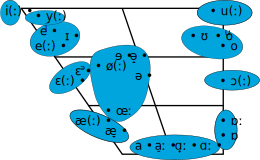
\includegraphics[width=.8\textwidth]{graphics/vowelcharts/bothoa-oral-vowels}
    \caption{Phonologically oral vowels in Bothoa Breton: principal allophones}
  \label{fig:bothoa-oral-vowels}
\end{figure} In the absence of actual formant data, the figure should be considered purely illustrative. Nevertheless, it does capture some of the extent of variation found in the dialect. (All the vowel charts in this section are adapted from \citeauthor{humphreys95:_phonol_bothoa_saint_nicol_pelem} \cite*{humphreys95:_phonol_bothoa_saint_nicol_pelem}, p.~73.)

\subsubsection{Nasal vowels}
\label{sec:nasal-vowels}

The dialect of Bothoa has six nasal vowels. According to \citet{humphreys95:_phonol_bothoa_saint_nicol_pelem}, nasal vowels are phonetically distinct from contingently nasalized vowels, which realize phonologically oral vowels adjacent to nasal consonants; presumably this corresponds to something like the difference between nasal vowels in French and nasalized vowels in English \citep{cohn90:_phonet,cohn93:_nasal_englis}.

All nasal vowels except \ipa{/ã/} do not enter into length contrasts. That is, long and short nasal vowels (except \ipa{/ã/}) are not used to implement lexical contrast, and phonetically long nasal vowels do not attract stress as long oral vowels do (\cref{sec:nasal-vowels-1}).

The high front nasal vowel \ipa{[ĩ]} is a nasalized version of cardinal \ipa{[i]}. It appears in about a dozen words, and occasionally the relevant lexical items can have oral \ipa{[i]} instead.

\ex.\a.\a.[]\twe{[ˈhĩːʃəw]}{henchoù}{roads}
\z.\b.\a.\twe{[ˈhĩːʒal]}{hejañ}{shake}
\b.\mbi{[ˈhiʒal]}

The mid-high nasal vowel \ipa{/ẽ/} is attested in about twenty lexical items. It is realized as a slightly dipthongized vowel \ipa{[ẽ\textsuperscript{ĩ}]}, in parallel with the diphthongized realization of long \ipa{/eː/} as \ipa{[e\textsuperscript{i}]}.

\ex.\a.\twp{ˈkwẽ\textsuperscript{ĩ}\kern-1pt vo}{koeñviñ}{to swell}
\b.\twp{ˈblẽ\textsuperscript{ĩ}\kern-1pt ʒal}{bl\^ejal}{moo}

The low front nasal vowel \ipa{[æ̃]} corresponds to the modern French pronunciation of the vowel in words such as \emph{bain}. It is overwhelmingly attested in borrowings from French.

\ex.\a.\twe{[ˈtræ̃]}{tren}{train (French \emph{train})}
\b.\twe{[ˈbasæ̃]}{basin}{pond; pool; bowl (French \emph{bassin})}


The front rounded nasal vowel \ipa{[ø̃]} is found in about a dozen lexical items. In a few words it alternates freely with an oral \ipa{[ø]}.

\ex.\a.\a.[]\twe{[ˈzø̃ːn]}{sizhun}{week}
\z.\b.\a.\twe{[ˈmøːz̥]}{meuz}{dish, delicacy}
\b.\mbi{[ˈmø̃ːz̥]}

The back mid rounded nasal vowel \ipa{/õ/} is described as significantly lower than the nasalized allophone of the mid high vowel \ipa{[o]}. It is attested in around twenty lexical items, but it is also used in borrowings from French.

\ex.\a.\twp{ˈpɔ̃ːʃəw}{ponchoù}{bridges}
\b.\twp{tɔ̃ːj̃\kern-1pt əw}{tonioù}{tunes}

Finally, the low nasal vowel \ipa{/ã/} is amply attested not only in roots, but in a number of productively used suffixes, and accounts for the vast majority of nasal vowel tokens. It is described as the nasalized correspondent of the back low unrounded vowel \ipa{[ɑ]}.

\ex.\a.\twp{ˈmɑ̃m}{mamm}{mother}
\b.\twp{ˈbrasɑ̃}{brasañ}{biggest}

It has a dipthongized allophone \phonint{ɑ̃\textsuperscript{õ}}, used word-finally in stressed position and, by some speakers, before the sequence of \phonint{ŋ} and a dorsal stop.

\ex.\a.\a.\twp{klɑ̃\textsuperscript{õ}}{klañv}{ill}
\b.\twp{ˈhɑ̃\textsuperscript{õ}}{hañv}{summer}
\z.\b.\a.\twp{ˈstɑ̃ŋɡ̊}{stank}{pond}
\b.\mbp{ˈstɑ̃\textsuperscript{õ}ŋɡ̊}

The low vowel is the only nasalized vowel to enter a length contrast, as the following examples demonstrate.

\ex.\a.\twp{ˈlɑ̃n}{lann}{gorse bush}
\b.\twp{ˈlɑ̃ːn}{leun}{full}

The set of nasal vowels in the dialect is shown in \cref{fig:bothoa-nasal-vowels}.

\begin{figure}[htp]
  \centering
  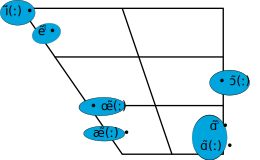
\includegraphics[width=.8\textwidth]{graphics/vowelcharts/bothoa-nasal-vowels}
  \caption{Nasal vowels in Bothoa Breton}
  \label{fig:bothoa-nasal-vowels}
\end{figure}

\subsubsection{Diphthongs}
\label{sec:diphthongs}

\citet{humphreys95:_phonol_bothoa_saint_nicol_pelem} identifies the following diphthongs in the Bothoa dialect: \phonint{ɛĭ}, \phonint{əy̆}, \phonint{əŭ} or \phonint{æŭ} (depending on the speaker), \phonint{aŭ}, and \phonint{ɑ̃w̃}. These are exemplified below.

\ex.\a.\a.[]\twp{ˈsɛĭz̥}{seizh}{seven}
\z.\b.\a.[]\twp{ˈəy̆n}{evn}{bird}\footnote{This word, along with its plural \phonint{ˈəy̆nəd̥}, is the only example of this diphthong in the dialect    \citep[p.~120]{humphreys95:_phonol_bothoa_saint_nicol_pelem}.}
\z.\b.\a.\twp{ˈdəŭ}{daou}{two (m.)}
\b.\mbp{ˈdæŭ}
\z.\b.\a.[]\twp{ˈdaŭr}{dour}{water}
\z.\b.\a.[]\twp{ˈdɑ̃w̃ʒər}{tavañjer}{apron}


\begin{figure}[htp]
  \centering
  
\includegraphics[width=.8\textwidth]{graphics/vowelcharts/bothoa-diphthongs}
  \caption{Diphthongs in Bothoa Breton}
  \label{fig:bothoa-diphthongs}
\end{figure}

\subsection{Consonants}
\label{sec:consonants-3}

The  phonetic inventory of consonants attested in Bothoa Breton is shown in \cref{tab:bothoa-cons-phonet},  which reproduces (with typographic changes) the table given by \citet[p.~123]{humphreys95:_phonol_bothoa_saint_nicol_pelem} and shows the set of \emph{phonetic} segments, \ie it lists the symbols needed in a narrow transcription.

\begin{sidewaystable}
  \centering
  \begin{tabular}{lccccccccccccc}
      \toprule
      & \multicolumn{2}{c}{Labial} & \multicolumn{4}{c}{Coronal} & \multicolumn{2}{c}{Palatal} &  &  &  &  \\
      \cmidrule{2-3}\cmidrule{4-7}\cmidrule{8-9}
      Manner & \hypcell[4em]{Labio\-dental} & Bilabial & Dental & Alveolar & \hypcell[4em]{Palato\-alveolar} & \hypcell[4em]{Alveo\-palatal} & Palatal &       \hypcell[4em]{Palatal-labial}  & Velar & Uvular & Pharyngeal & Glottal \\
      \midrule
      Stop & & \ipa{p~b} & \ipa{t~d} & & & \ipa{tʲ~dʲ} & \ipa{c~ɟ} & & \ipa{k~ɡ} \\
      Affricate & & & & & & \ipa{tɕ~dʑ} \\
      Fricative & \ipa{f~v} & & & \ipa{s~z} & \ipa{ʃ~ʒ} & \ipa{ɕ~ʑ} & \ipa{ç~j} & & \ipa{x~ɣ} & \ipa{\phantom{χ}~(ʁ)} & \ipa{ħ} & \ipa{h~ɦ} \\
      Nasals & \ipa{ɱ} & \ipa{m~m̥} & \ipa{n~n̥} & & & \ipa{ɲ~ɲ̥} & \ipa{j̃} & & \ipa{ŋ~ŋ̊} \\
      Laterals & & & \ipa{l~l̥} \\
      Rhotics & & & & \ipa{r~r̥} \\
      Approximants & & \ipa{w~w̥} & & & \ipa{j̃} & \ipa{ç~j} & & \ipa{ɥ} & & \ipa{(χ̞)~(ʁ̞)} \\
\bottomrule
  \end{tabular}
  \caption{Consonants: phonetic inventory}
  \label{tab:bothoa-cons-phonet}
\end{sidewaystable}

\subsubsection{The phonetic realization of consonants}
\label{sec:phon-real-cons}

The stops \ipa{[p~t~k]} and \ipa{[b~d~ɡ]} and the affricate pair \ipa{[ʧ~dʒ]} are distinguished by  voicing; the voiceless stops are said to lack noticeable aspiration (\foreigntextquote{french}{sans aspiration notable}).\footnote{The phonetic study of the west Cornouaillais dialect of Argol by \citet{Bot82} also shows full voicing of stops.} Minimal pairs are shown in \cref{ex:bothoa-voicing-minpairs}.

\ex.\label{ex:bothoa-voicing-minpairs}\a.\a.\twp{ˈboɫx}{boulc'h}{first cut}
\b.\twp{ˈpoɫx}{polc'h}{bug}
\z.\b.\a.\twp{ˈdiː}{div}{two (f.)}
\b.\twp{ˈtiː}{ti}{house}
\z.\b.\a.\twp{ˈɡãːnət}{ganet}{born}
\b.\twp{ˈkãːnət}{kanet}{sung}

The velar stops \ipa{[k~ɡ]} have fronted allophones, which \citet{humphreys95:_phonol_bothoa_saint_nicol_pelem} writes as \ipa{[c~ɟ]} and describes as \enquote{mediopalatal} (\textfrench{\emph{médio-palatale}}). These are found before the segment \ipa{[i]}. I assume they represent the same phonological segment as \ipa{[k]} and \ipa{[ɡ]} and thus will transcribe them as \ipa{[kʲ~ɡʲ]}. The main reason is that there no evidence for a phonological distinction between \ipa{[k~ɡ]} and \ipa{[kʲ~ɡʲ]}. The decision is also supported by the fact that nasals are realized as \phonint{ŋ} and not \phonint{ɲ} before these segments. Some examples are given in \ref{ex:bothoa-ki-exx}.

\ex.\label{ex:bothoa-ki-exx}\a.\twp{ˈlakʲiãm}{lakiamp}{we will put}
\b.\twp{akʲ i ˈziː}{hag he zi}{and her house}
\b.\twp{ˈvrãŋkʲiz̥}{frankiz}{open space, the outdoors}
\b.\twp{ˈklɒːɡʲiad̥}{klogiad}{ladleful}

The affricates \phonint{tɕ} and \phonint{dʑ} are described as similar to the  Polish orthographic \emph{\'c}, \emph{d\'z}. I will use the symbols \ipa{[ʧ~dʒ]} throughout for convenience.

\ex.(Near-)minimal pairs for velars
\a.\a.\twp{ˈʧɛĭsə}{keid-se}{so far}
\b.\twp{ˈkɛĭn}{kein}{back}
\z.\b.\a.\twp{ˈdʒaz̥}{degas}{bring}
\b.\twp{ˈɡaz̥}{gas}{send (mutated form)}

\label{bothoa-phonetic-palatalization}Segments acoustically similar to \phonint{ʧ} and \phonint{dʒ} may also appear as the extremes of a continuum of variable realizations corresponding to the sequence of a coronal stop and the vowel \ipa{[i]} before another vowel, as in \cref{ex:bord}.

\ex.\label{ex:bord}\a.\a.\twp{ˈbɒrd̥}{bord}{side}
\b.\twp{ˈbɒrdʒəw}{bordoù}{sides}
\b.\mbp{ˈbɒrdiəw}
\z.\b.\label{ex:rastel-kontel}\a.\twp{ˈkonˌtɛl}{kontel}{knife}
\b.\twp{ˈkontiəw}{kontilli}{knives}
\b.\mbp{ˈkontjəw}
\b.\mbp{ˈkonʧəw}


The fricatives \ipa{[f~v]}, \ipa{[s~z]} and \ipa{[ʃ~ʒ]} are said to be similar to their French counterparts. \mbox{(Near-)}minimal pairs are given in the examples below.

\ex.\a.\a.\twp{ˈvãmin}{binim}{venom}
\b.\twp{ˈfãmin}{famin}{hunger}
\z.\b.\a.\twp{ˈzel}{sell}{look}
\b.\twp{ˈsel}{}{(bike) saddle (French \emph{selle})}
\z.\b.\a.\twp{ˈʒakəz̥}{Jakez}{oaf}
\b.\twp{ˈʃakəd̥}{choked}{crumpled}


In preconsonantal contexts, \ipa{/s/} (or \ipa{/z/}) may alternate with \ipa{[h]} (phonetically normally \phonint{ħ} in this position). This is especially frequent with the prefix \preff{diz} (\preff{dis}).

\ex.\label{dislivan-dismantran}\a.\a.\twp{ˌdisˈliːvo}{dislivañ}{discolour}
\b.\mbp{ˌdiħˈliːvo}
\z.\b.\a.\twp{ˈdiħmɑ̃nt}{dismantrañ}{waste}
\b.\mbp{ˈdismɑ̃nt}

The alternation does not appear to be systematic, but is lexicalized in one case.\footnote{According to \citet[p.~168]{humphreys95:_phonol_bothoa_saint_nicol_pelem}, neither *\phonint{ˈr̥ɑːx} nor *\phonint{ˈr̥ɑːzəd̥} are possible in the dialect.}

\ex.\a.\twp{ˈr̥aːz̥}{razh}{rat}
\b.\twp{ˈr̥aːɦəd̥}{razhed}{rats}


The fricatives \ipa{[ʃ]} and \ipa{[ʒ]} do not appear to participate in variation with coronal fricatives parallel to that shown in \cref{ex:bord}, as shown in \cref{ex:morzel-brezel}.

\ex.\label{ex:morzel-brezel}\a.\twp{ˈmɒrˌzɛl}{morzhol}{hammer}
\b.\twp{ˈmɒrziəw}{morzholioù}{hammers}
\b.\mbp{ˈmɒrzjəw}
\b.*\mbp{ˈmɒrʒəw}

The fricative that \citet{humphreys95:_phonol_bothoa_saint_nicol_pelem} transcribes phonologically as \ipa{[h]} has a number of realizations. The voiceless glottal phonation \phonint{h} is found word-initially, word-medially following \ipa{[l~r]}, and immediately before the vowel bearing the main stress. The breathy voiced phonation \phonint{ɦ} is normally found intervocalically, and occasionally word-initially. The voiceless velar fricative \phonint{x} is found utterance-finally and before a voiceless consonant, while its voiceless correspondent \phonint{ɣ} is a rare variant noted word-finally in sandhi before \ipa{[m~v]}. Finally, the pharyngeal \phonint{ħ} is the most common preconsonantal variant, alternating freely with \phonint{x} and \phonint{ɣ}. Examples are given in \cref{ex:bothoa-h-exx}.

\ex.\label{ex:bothoa-h-exx}\a.\a.\twp{ˈhɛĭ}{heiz}{barley}
\b.\twp{ˈmarhəw}{marc'hoù}{stallions}
\z.\b.\a.\twp{ˈzɛɦo}{sec'hañ}{to dry}
\b.\twp{o ˈzaːɦ e}{ur sac'h eo}{(it) is a bag}
\z.\b.\a.\twp{o ˈplɑːx}{ur plac'h}{a girl}
\b.\twp{o ˌplɑːx ˈpəŭr}{ur plac'h paour}{a poor girl}
\z.\b.\a.\twp{ə ˈvjɒɣmə}{ar vuoc'h-mañ}{this cow}
\z.\b.\a.\twp{dæħˈmɑːt}{dalc'hmat}{always}
\b.\twp{o ˌvjɒħ ˈlart}{ur vuoc'h lart}{a fat cow}

\enquote{Occasionally} this fricative may also alternate with \ipa{[s]} (the precise nature of the variation is not described). The pattern is reminiscent
of that described above for \ipa{[s]} and \ipa{[z]} (as in \cref{dislivan-dismantran}).

\ex.\a.\a.\twp{ˈzɛːx}{sec'h}{dry}
\b.\twp{ˈzɛstər}{sec'hder}{dryness}
\b.\mbp{ˈzɛħtər}
\z.\b.\a.\twp{ˌdɛstəˈnoːs}{dec'h-da-noz}{tonight}
\b.\twp{dɛːx}{dec'h}{today}

The nasals \ipa{[m]} and \ipa{[n]} do not present significant difficulties. The nasal \ipa{[ŋ]} is only encountered before velar stops.

\ex.\a.\a.\twe{[ˈmãn]}{mann}{nothing}
\b.\twe{[ˈnãn]}{nann}{no}

The segment that \citet{humphreys95:_phonol_bothoa_saint_nicol_pelem} interprets as a phonological palatal nasal \ipa{[ɲ]} is realized as \phonint{ɲ} word-medially following \phonint{r} and \phonint{j}; in all other contexts, it is realized as a nasalized palatal glide \phonint{j̃\kern-1pt}, and these two segments are in free variation following \ipa{[w]}. Neither is found word-initially.

\ex.\a.\twp{ˈpwiːj̃\kern-1pt al}{poaniañ}{to upset}
\b.\twp{ˈkɛjɲəw}{keinioù}{backs}
\b.\twp{ˈtõj̃\kern-1pt əw}{tonioù}{tunes}
\b.\twp{ˈhãwɲo}{anvel}{to call, name}
\b.\mbp{ˈhãwj̃\kern-1pt o}


The phonetic segment \phonint{ɲ} can also appear as the member of a continuum of possible realizations, from \ipa{[ni]} through \ipa{[nj]} and \ipa{[nʲ]} to \ipa{[ɲ]}, as in \cref{binied}.

\ex.\label{binied}\a.\twp{ˈbiːniəd̥}{benniget}{blessed}
\b.\mbp{ˈbiːnĭəd̥}
\b.\mbp{ˈbiːnjəd̥}
\b.\mbp{ˈbiːɲəd̥}


The lateral \ipa{[l]} is normally similar to the French \ipa{[l]}. It demonstrates minor coarticulation effects. Specifically, the initial portion of the sonorant may be devoiced following voiceless stops (consistent with the description of voiceless stops as short-lag VOT segments). The lateral is slightly palatalized before \ipa{[i]} and slightly velarized before \ipa{[u]}. A more strongly velarized \ipa{[ɫ]} is found before \phonint{h} and \phonint{x}, as shown in \cref{ex:bothoa-dark-l}.\footnote{The association between \ipa{[h]} and velarized \phonint{ɫ} should perhaps be compared to the possible realization of \ipa{[rh]} as \phonint{xː} (see \cref{erch-chwech}). The class of \ipa{[h]} and (coda) \ipa{[l~r]} as velarized consonants (which may also exert a backing influence on preceding vowels) is reminiscent of the Old English \enquote{breaking}, \ie the appearance of a back glide before \ipa{[h]} (phonetically \phonint{h} and \phonint{x}) and coda \ipa{[l]} and \ipa{[r]}; see \citet[§§5.16\endash5.34]{hogg92:_old_englis}. It appears that breaking did not play an important rôle in the synchronic phonology of Old English \citep[§5.32]{hogg92:_old_englis}, but the precursors to the sound change may have been similar to the situation seen in Breton.}

\ex.\label{ex:bothoa-dark-l}\a.\twp{ˈbɔɫx}{boulc'h}{first cut}
\b.\twp{ˈmɔɫhəd̥}{moualc'hoù}{swallows}

The rhotic, for which I used the cover symbol \ipa{[r]}, is realized in a variety of ways. In the conservative variety (speakers born before 1920), it is normally an apical tap or trill, with the tap being the dominant pronunciation and the trill only found word-initially. It can be voiceless, especially following an initial voiceless stop. In newer varieties, it is realized either as a uvular fricative \ipa{[ʁ]}, or as a uvular approximant \ipa{[ʁ̞]} (also possibly devoiced to a relatively frictionless \ipa{[χ̞]}).

The approximants \ipa{[w~j~ɥ]} are described as generally similar to the corresponding French sounds as in \emph{oiseau}, \emph{hier}, \emph{huit}. They are slightly devoiced following voiceless consonants.

Finally, Bothoa Breton possesses a set of voiceless sonorants \ipa{[m̥~n̥~l̥~r̥~w̥~ɥ̊]}. In addition, \ipa{[ç]}, as we shall see below, stands in the same relationship to \ipa{[j]} as voiceless sonorants do to voiced ones. The phonetic realization of these segments was studied by \citet{humphreys}. He found that \ipa{[m̥]}, \ipa{[n̥]} and \ipa{[l̥]} can be broken up into a voiceless and a voiced portion, so \phonint{m̥m}, \phonint{n̥n} and \phonint{l̥\kern-1pt l}. The palatal-labial voiceless glide \ipa{[ɥ̊]} is extremely rare; the voiceless palatal \ipa{[ç]} is described as similar to the German \emph{ich-Laut}, and \ipa{[w̥]} is said to be similar to the \ipa{[ʍ]} of certain English dialects. Finally, the realization of \ipa{[r̥]} varies: some speakers have a voiceless tap or trill \phonint{r̥} similar to Welsh \emph{rh}, and others have a uvular fricative \phonint{χ}.

\subsubsection{Word-final phonetics and sandhi}
\label{sec:word-final-phonetics}

The realization of consonants, and especially obstruents, in phrasal contexts is often different from that found in lexical contexts; this is particularly true in utterance-final position. The phonetic alternations can be broadly classified into two groups: lack of release and loss of laryngeal specification.

\paragraph{Lack of release}
\label{sec:lack-release}

Word-final stops, whether before a pause or before another consonant, are often unreleased, which can even lead to confusion as to the identity of the final stop:

\ex.\a.\a.[]\twp{ˈdib̥̚}{dibr}{saddle}
\z.\b.\a.[]\twp{o ˈhad̥̚}{ur c'had}{a hare}
\z.\b.\a.[]\twp{ˈɡwɑːɡ̊̚}{gwak}{weak}
\z.\b.\a.\twp{ˈr̥iːdəɡ̊̚}{redek}{run}
\b.\mbp{ˈr̥iːdəd̥̚}


In word-final nasal\endash stop sequences, not only can the stop remain unreleased, but also the nasal may be realized with greater duration. If an underlyingly voiceless stop is deleted or obscured in this manner, the nasal is also often, though not necessarily, voiceless (except before a voiced segment). The appearance of stops is especially disfavoured before another consonant

\ex.\label{bothoa-pont-et-al}\a.\a.\twp{o ˈpont}{ur pont}{a bridge}
\b.\mbp{o ˈpont̚}
\b.\mbp{o ˈpon̥}
\b.\mbp{o ˈponː}
\b.\twp{o ˌponː ˈkoːz̥}{ur pont kozh}{an old bridge}
\b.\mbp{o ˌpon ˈkoːz̥}
\z.\b.\a.\twp{ˈdɛnt}{dent}{teeth}
\b.\twp{ˌdɛn ˈbrɑː}{dent brav}{good teeth}
\b.\mbp{ˌdɛnː ˈbrɑː}
\z.\b.\a.\twp{on ˈdɑ̃nd al}{un dant all}{another tooth}
\b.\mbp{on ˈdɑ̃nː al}

A similar phenomenon involving the loss of the stop articulation and a lengthening of the preceding consonant is found in obstruent sequences, in practice limited to sequences of \ipa{[s]} and a stop:

\ex.\a.\a.[]\twp{ˈtrist e}{trist eo}{[it] is sad}
\z.\b.\a.\twp{ˌlɒst ˈhiːr}{lost hir}{a long tail}
\b.\mbp{ˌlɒsː ˈhiːr}
\b.\mbp{ˌlɒs ˈhiːr}
\z.\b.\a.\twp{ˈʒist}{chistr}{cider}
\b.\mbp{ˈʒisː}
\z.\b.\a.\twp{ˈʒisː ˈkaləd̥}{chistr kalet}{hard cider}
\b.\mbp{ˈʒis ˈkaləd̥}


Final coronal stops may disappear from the acoustic record before another consonant: this is said to be obligatory in unstressed syllables (\cref{ex:evid-mirout-boued}) and \enquote{sporadic} in stressed ones (\cref{ex:koad-lokeltaz}).

\ex.\label{ex:evid-mirout-boued}\a.\twp{vid̥}{evit}{for, in order to}
\b.\twp{miːrəd̥}{mirout}{keep, look after}
\b.\twp{vi ˌmiːrə ˈbwid̥}{evit mirout boued}{in order to watch the food}

\ex.\label{ex:koad-lokeltaz}\a.\twp{ˈkwɛd̥}{koad}{forest}
\b.\twp{ˌkwɛ loɡəˈtaːz̥}{koad Lokeltaz}{the forest of Locqueltas}

When two identical consonants straddle a word boundary, the result is either a \enquote{slightly geminated} articulation when both consonants belong to stressed syllables (\cref{ex:koad-derv}); in other positions the result is said to be indistinguishable from a single consonant (\cref{ex:ar-parrez-se}).

\ex.\a.\label{ex:koad-derv}\a.\twe{/kwæd/}{koad}{wood}
\b.\twp{ˌkwædˈdær}{koad derv}{oak}
\z.\b.\label{ex:ar-parrez-se}\a.\twe{/paruz/}{parrez}{parish}
\b.\twp{ə ˈbarusə}{ar barrez-se}{this parish}

\paragraph{Laryngeal phenomena}
\label{sec:laryngeal-phenomena}

Word-finally, the contrast between voiced and voiceless obstruents is suspended. However, the outcome of this suspension depends on the phonetic context.

\subparagraph{Final laryngeal neutralization}
\label{sec:final-laryng-neutr-phon}

I use the term \enquote{final laryngeal neutralization} \citep[\cfm][]{iverson11:_final} to refer to the fact that both voiced and voiceless obstruents exhibit what \citet[p.~190]{humphreys95:_phonol_bothoa_saint_nicol_pelem} calls the \enquote{voiceless realization} before a pause (\ie phrase-finally). Fully voiced obstruents are entirely absent from this position. However, according to \citet{humphreys95:_phonol_bothoa_saint_nicol_pelem}  the actual realization is not necessarily identical to that of true voiceless obstruents:

\blockquote{It should be pointed out that the alternation between voiced and voiceless segments, which represents the most important category of these [sandhi] modifications, is, from the phonetic point of view, not a simple binary choice: quite often one encounters not just voiceless lenes, but also consonants with a decrease in voicing. The faster the speech rate and the more relaxed the articulation, the more pronounced are the assimilations.\footnote{\foreigntextquote{french}{Il faut se rappeler [\ldots] que l'alternance sourde/sonore, qui représente la catégorie plus importante de ces modifications, n'est pas, sur le plan phonétique, un simple choix binaire: on rencontre assez souvent, non seulement des sourdes douces, mais aussi des consonnes à sonorité décroissante. Plus le débit rapide et l'articulation relâchée, plus les assimilations sont poussées.}}}

Of course, only instrumental study could clarify the correctness, and in fact the true empirical content of this description. Still, the realization of obstruents devoiced by sandhi is apparently nor identical to that of lexical voiceless obstruents. Consequently, I use the devoicing diacritic for prepausal obstruents in both phonetic and surface\hyp phonological transcription. (Phonological arguments for a distinction are provided below, see especially \cref{sec:except-devo-sandhi}.) Two examples are shown in \ref{ex:bothoa-findev}, together with forms without neutralization which demonstrate the underlying laryngeal specification:

\ex.\label{ex:bothoa-findev}\a.\a.\twp{ˈkɔɡ̊}{kog}{rooster}
\b.\twp{ˈkɔɡəw}{kogoù}{forests}
\z.\b.\a.\twp{ˈtɔɡ̊}{tog}{hat}
\b.\twp{ˈtɔkəw}{togoù}{hats}

\subparagraph{Sandhi voicing}
\label{sec:sandhi-voicing-phon}

When an obstruent is not final in the phrase and is followed by a sonorant, a vowel, or a voiced obstruent, it is generally realized with voicing irrespective of its underlying laryngeal specification. Examples of this are shown in \cref{ex:bothoa-sandhi-voi}.

\ex.\label{ex:bothoa-sandhi-voi}\a.\a.\twp{kɔɡ̊}{kog}{rooster}
\b.\twp{o ˌhɔk ˈtrøt}{ur c'hog treut}{a skinny rooster}
\b.\twp{ˌkɔɡ izˈmaːj}{kog If-Mai}{Yves-Marie's rooster}
\z.\b.\a.\twp{tɔɡ̊}{tog}{hat}
\b.\twp{on ˌtɔk ˈʃik}{un tog chik}{a chic hat}
\b.\twp{on ˈtɔɡ ˌal}{un tog all}{another hat}
\b.\twp{ˌtɔɡ ˈʒãː}{tog Yann}{Jean's hat}

\enquote{Quite often} (\foreigntextquote{french}{assez souvent}) the underlying voiceless fricatives \ipa{/f/}, \ipa{/s/}, and \ipa{/ʃ/}, when preceded by short vowels, resist the voicing in the relevant context. It is not clear whether this resistance is a property of lexical items or whether the same lexical item can appear in both forms. \citet{humphreys95:_phonol_bothoa_saint_nicol_pelem} says that examples like those in \cref{ex:bothoa-vcl-fricative-voicing} \enquote{coexist} with those in \cref{ex:bothoa-vcl-fricative-no-voicing} (all the relevant words end in lexical voiceless obstruents).

\ex.\a.\label{ex:bothoa-vcl-fricative-voicing}\a.\twp{o ˈprøz wæ}{ur pres a oa}{it was a cupboard}
\b.\twp{o ˈpeʒ laˈpiːnəd̥}{ur pech lapined}{a rabbit trap}
\z.\b.\label{ex:bothoa-vcl-fricative-no-voicing}\a.\twp{on ˈtas wæ}{un tas a oa}{it was a cup}
\b.\twp{on ˈhaʃ ˈlem}{un hach lem}{a well-sharpened axe}

As for final consonant sequences, \citet[p.~196]{humphreys95:_phonol_bothoa_saint_nicol_pelem} distinguishes three types of realizations before vowels:

\begin{itemize}
\item If the first element is a liquid,  word-final obstruents behave exactly as if they followed a vowel.
\item In the case of sequences of the type \enquote{nasal + stop}, the situation is complicated by the fact that, as discussed above (see \cref{bothoa-pont-et-al} on p.~\pageref{bothoa-pont-et-al}), these tend to undergo some sort of progressive assimilation in terms of nasality, losing the burst. Nevertheless, as that example shows, if the stop is not deleted or obscured in such sequences, it can be realized with voicing.
\item In sequences of the type \enquote{\ipa{/s/} + stop} (where the majority are of the form \ipa{/st/}), dropping of the final consonant is common (especially before a consonant, as is the case for stops generally). Interestingly, even if the stop disappears from the acoustic record, pre-sonorant (or at least prevocalic) voicing of such sequences is quite uncommon: while realizations like that in \cref{ex:chistr-all} do exist, \citet{humphreys95:_phonol_bothoa_saint_nicol_pelem} attributes them to changes in the underlying form (so that \eg `cider' is underlyingly \ipa{/ʒis/} rather than \ipa{/ʒist/}). However, voicing assimilation is possible before obstruents. The segment \ipa{[h]} inhibits pre-sonorant voicing.

\end{itemize}

\ex.\a.\a.\twp{ˈlɒst}{lost}{tail}
\b.\twp{ˈlɒst ˈhiːr}{lost hir}{long tail}
\b.\mbp{ˈlɒsː ˈhiːr}
\b.\twp{o ˌlɒzd ˈbɛːr}{ul lost berr}{a short tail}
\b.\mbp{o ˌlɒzː ˈbɛːr}
\b.\mbp{o ˌlɒz ˈbɛːr}
\z.\b.\a.\twp{ˈʒist}{chistr}{cider}
\b.\mbp{ˈʒisː}
\b.\twp{ˌʒis ˈkalət}{chistr kalet}{strong cider}
\b.\mbp{ˌʒisː ˈkalət}
\b.\label{ex:chistr-all}\twp{ˈʒiz ˈal}{chistr all}{another cider}
\z.\b.\a.\twp{ˈtrist}{trist}{sad}
\b.\twp{ˈtrist e}{trist eo}{[it] is sad}

\paragraph{Miscellaneous sandhi changes}
\label{sec:misc-sandhi-chang}

Other postlexical alternations are possible, but are described as irregular.

Final obstruents may be fully or partially nasalized before other nasals:

\ex.\a.\twp{ˈzæːb̥}{sabl}{sand}
\b.\twp{ˌzæːb ˈnæd e}{sabl naet eo}{(it) is proper sand}
\b.\mbp{ˌzæːm ˈnɛd e}

The affricates may lose their fricative portion before a consonant to be realized as something like palatalized coronal (\cref{ex:bothoa-ts-to-t}) or dorsal (\cref{ex:bothoa-ts-to-k}) stops.

\ex.\a.\label{ex:bothoa-ts-to-t}\a.\twp{ˌʧitʲ ˈpwɛːz̥}{kig poazh}{roasted meat}
\b.\twp{ˌʧidʲ ˈbærəd̥}{kig berved}{boiled meat}
\z.\b.\label{ex:bothoa-ts-to-k}\a.\twp{ˌʧiɡ ˈɡad̥}{kig gad}{hare meat}
\b.\twp{ˌʧik ˈr̥ɒstəd̥}{kig rostet}{roasted meat}

Very sporadically, underlying \ipa{/s/} and \ipa{/z/} may be realized as \ipa{[h]} before a sonorant (recall that this can also happen lexically):

\ex.\a.\a.\twp{ˈhõz̥}{honnezh}{this one there}
\b.\twp{ˌhõh wæ ˈbraːz̥}{honnezh a oa braz}{it was big}
\z.\b.\a.\twp{ˈmeməz̥}{memes}{same}
\b.\twp{ˌmemə m̥\kern1pt ɔd̥}{memes mod}{the same way}



\subsection{Phonological inventories}
\label{sec:phon-invent}

The phonemicization of Bothoa Breton segments appears mostly straightforward. In this section I discuss some outstanding issues.


\subsubsection{The status of the schwa}
\label{sec:status-schwa}

The phonemic status of the distinction between \ipa{[ə]} and \ipa{[ø]}/\ipa{[œ]} is difficult to determine, which is similar to the situation in French. It is certainly not used to implement lexical contrast, since the segments stand in (almost) complementary distribution: there is one instance (secondary stress on final syllables) where different speakers use different phones (some use a more like \ipa{[ø]}-like segment in this position). The complementary distribution could in principle be due either to \ipa{[ə]} and \ipa{[ø]} being two different phonological symbols (in which case the inter-speaker variation in the case of final syllables could be due to some phonological difference in how that position is represented) or to a language\hyp particular aspect of phonetic implementation.

Arguments for the former view are difficult to come by, since both \phonint{ə} and (especially) \phonint{œ} are quite inert phonologically. The only argument for a phonological distinction is its categoricity. However, categorical distributions in the data may well arise from non-phonological factors (\cref{sec:relev-categ-distr}). Moreover, in the absence of instrumental data we cannot  say for sure that the distinction is implemented categorically: in fact, given the relatively wide range of possible phonetic realizations of \ipa{[ə]} (cf.\ \cref{fig:bothoa-oral-vowels} on p.~\pageref{fig:bothoa-oral-vowels}), it appears possible that the realizations of \ipa{[ø]} and \ipa{[ə]} may actually be forming a continuum.

The evidence is thus indeterminate.\footnote{\citet[p.~108]{humphreys95:_phonol_bothoa_saint_nicol_pelem} treats \ipa{[ø]} and \ipa{[ə]} as a single phoneme, on the basis of the complementary distribution. He also observes that when the melody in a song requires prolonging a syllable with a schwa, Bothoa speakers will use a front rounded vowel (he notes that speakers to the west of Bothoa use \ipa{[ɛ]} in similar situations). However, it is not entirely clear whether these facts are linguistically relevant. In particular, \citet{humphreys95:_phonol_bothoa_saint_nicol_pelem} transcribes the relevant example with a stress mark on the schwa-containing syllable: \phonint{kɑ̃ˈnøːːt} `sung' (normally \ipa{[ˈkãːnəd̥]}). I leave this matter aside here.} Moreover, there is a distinct possibility that, given the absence of strong evidence either way, different learners may actually converge on different mental grammars that would both be relatively well compatible with the relevant ambient data. In the absence of firm evidence for a phonological contrast, I follow \citet{humphreys95:_phonol_bothoa_saint_nicol_pelem} in treating \ipa{[ə]} and \ipa{[ø]} as the same phonological segment. I will transcribe it as \ipa{[ə]} in purely phonological contexts (\eg when describing feature specifications), but will keep \ipa{[ø]} in surface-phonological transcriptions of words to keep them closer to the phonetics.\footnote{A third potential solution is proposed by \citet{le00:_le_malguen} for the dialect of Malguénac, where similar facts obtain with respect to the complementary distribution of \phonint{œ} and \phonint{ə}: working in a structuralist framework, \citeauthor{le00:_le_malguen} proposes to treat surface \ipa{[ə]} as representing phonemic \ipa{/œ/} when there is evidence from alternations and as phonemic \ipa{/ə/} when the relevant vowel never alternates with \ipa{[œ]}. However, this solution again rests on a phonetic argument rather than a phonological one.}


\subsubsection{Consonants}
\label{sec:bothoa-consonant-dist}

The consonant inventory appears to be mostly unproblematic. The following remarks are in order:

\begin{itemize*}
\item The phonological segment that \citet{humphreys95:_phonol_bothoa_saint_nicol_pelem} transcribes as \ipa{/ɲ/} is realized as either \phonint{ɲ} or \phonint{j̃\kern-1pt}. Since \phonint{ɲ} can also be the realization of a \ipa{[ni]} sequence, I use \ipa{[j̃\kern-1pt]} in phonological transcription;
\item The rhotic has a range of coronal and uvular realizations varying across contexts and speakers. I use \ipa{[r]} throughout for simplicity;
\item I transcribe the affricates as \ipa{[ʧ]} and \ipa{[dʒ]} throughout, irrespective of their phonetic realization;
\item I ignore some assimilations that are clearly allophonic (\ie which do not involve changes of phonological symbols) such as the fronting of \ipa{[k]} and \ipa{[ɡ]} before front vowels;
\item I follow \citet{humphreys95:_phonol_bothoa_saint_nicol_pelem} in treating \ipa{[h]} as a single phonological symbol, despite the multitude of its realizations. Apart from the lack of phonological evidence, the reason for this decision is the fact that the variation is described as not being categorical, but rather appears to be driven by phonetic context.
\end{itemize*}

\Cref{tab:inventories-bothoa} shows the phonological inventories for Bothoa Breton I operate with in this thesis; the labels are to be taken as purely descriptive. For an explanation of the transcription of the voiceless sonorants, see \cref{sec:provection-sonorants}.

\begin{table}[htp]
\centering
\subtop[Vowel inventory]{%
  \begin{tabular}{lcccc}
    \toprule
& \multicolumn{2}{c}{Front} & Central & Back \\
\cmidrule{2-3}
Height & Unrounded & Rounded & & \\
\midrule
High & \ipa{i~iː} & \ipa{y~yː} & & \ipa{u~uː} \\
Mid-high & \ipa{e~eː} & & & \ipa{o~oː} \\
Mid & \ipa{ɛ~ɛː} & \ipa{ø~øː} & \ipa{ə} & \ipa{ɔ~ɔː} \\
Mid-low & \ipa{æ~æː} & & & \ipa{ɒ~ɒː} \\
Low & & & \ipa{a~aː} \\
\bottomrule
\label{tab:phonemic-vowels-bothoa}
  \end{tabular}%
}
\subtop[Consonant inventory]{%
  \begin{tabular}{lccccccc}
    \toprule
Manner & Labial & Coronal & Postalveolar  & \hypcell[4em]{Palatal\-labial} & Palatal & Dorsal & Glottal \\
\midrule
Stops & \ipa{p~b} & \ipa{t~d} & & &  & \ipa{k~ɡ} \\
Affricates & & & \ipa{ʧ~dʒ} \\
Fricatives & \ipa{f~v} & \ipa{s~z} & \ipa{ʃ~ʒ} & & & & \ipa{h} \\
Nasals & \ipa{m~hm} & \ipa{n~hn} & & & \ipa{j̃}  \\
Laterals & & \ipa{l~hl} \\
Rhotics & & \ipa{r~hr} \\
Approximants & \ipa{w~hw} & & & \ipa{ɥ~hɥ} & \ipa{j~hj} \\
\bottomrule
  \end{tabular}
}
  \caption{Inventories for Bothoa Breton}
\label{tab:inventories-bothoa}
\end{table}

In \cref{tab:transcription-bb} I summarize the transcription practice I use for surface\hyp phonological representations in this chapter.\begin{table}[tbp]
  \centering
  \adjustbox{width=\textwidth}{\begin{tabular}{*{2}{>{\ipafont}l}p{.6\textwidth}}
    \toprule
    Phonology & Phonetics & Comments\\
    \midrule
    {[p t ʧ k]} & \phonint{p t ʧ k(ʲ)} & Short-lag VOT, found word-finally only in exceptional cases \\
    {[b d dʒ ɡ]} & \phonint{b̬ d̬ d̬ʒ̬ ɡ̬(ʲ)} & Fully voiced stops, not found word\hyp finally \\
    {[b̥ d̥ d̥ʒ̊ ɡ̊]} &
    \begin{minipage}[t]{.2\linewidth}\raggedright
      \phonint{p/b̥/b(̚) t/d̥/d(̚) tʲ/d̥ʲ/dʲ/dʒ k/ɡ̊/ɡ(̚)}
    \end{minipage}
& Partially or fully voiced depending on context, possibly unreleased, found mostly word\hyp finally \\
    {[f s ʃ]} & \phonint{f s ʃ} & \\
    {[v z ʒ]} & \phonint{v̬ z̬ ʒ̬} & Fully voiced, not found word\hyp finally \\
    {[v̥ z̥ ʒ̊]} & \phonint{f/v̥/v s/z̥/z ʃ/ʒ̊/ʒ} & Partially or fully voiced depending on context, found word\hyp finally \\
    {[h]} & \phonint{h ɦ ħ ɣ} & Depending on context \\
    {[m n]} & \phonint{m n/ŋ} & No significant allophony described other than possible assimilation of \ipa{/n/} to \phonint{ŋ} \\
    {[l r]} & \phonint{l/ɫ ɾ/r/ʁ/χ} & Some velarization of \ipa{[l]}, between\hyp speaker variation in \ipa{[r]} \\
    {[j̃\kern-1pt]} & \phonint{j̃\kern-1pt{} ɲ} & Depending on context \\
    {[u/w i/j ɥ]} & \phonint{w j ɥ} & As with Welsh, I write \ipa{[w~j]} in onsets and \ipa{[i~u]} in nuclei despite the lack of a phonological distinction\\
    {[hm hn hl]} & \phonint{m̥\kern1pt m n̥n l̥\kern-1pt l/ɬ} & \multirow{2}{*}{See \cref{sec:provection-sonorants} for the phonological rationale}  \\
    {[hr hw hj hɥ]} & \phonint{r̥/χ ʍ ç ɥ̊} \\
    \bottomrule
  \end{tabular}
}  \caption{Transcription for Bothoa Breton}
  \label{tab:transcription-bb}
\end{table} In the next section I take up some issues in the suprasegmental phonology of Bothoa Breton, specifically stress, syllable structure, phonotactics, and the relationship between vowel length and laryngeal specification.

\section{Suprasegmental phonology}
\label{sec:supr-phon}

\subsection{Stress}
\label{sec:stress}

Unlike most other Brythonic varieties, in Bothoa Breton the placement of stress is not determined for the most part by top-down prosodic requirements. In this section I argue that stress placement in Bothoa Breton is mostly driven by lexical factors, mitigated by top-down requirements which include stressing the rightmost moraic trochee in a word and final-syllable stress.

\subsubsection{Types of stress}
\label{sec:types-stress}

According to \citet{humphreys95:_phonol_bothoa_saint_nicol_pelem}, stressed vowels are characterized by greater intensity, greater length and rising pitch (this latter especially pronounced on final syllables).

There is one type of words where the realization of stress is not entirely straightforward. According to \citet{humphreys95:_phonol_bothoa_saint_nicol_pelem}, there is a marked difference between two classes of disyllabic words, exemplified in \ref{ex:bothoa-double-peak}.

\ex.\label{ex:bothoa-double-peak}\a.\twe{[ˈpærson]}{person}{parson}
\b.\twe{[ˈdaˌvad̥]}{dañvad}{ewe}

If \posscite[']{humphreys95:_phonol_bothoa_saint_nicol_pelem} description is correct, in words of the first type intensity, length and pitch peaks all converge on the initial syllable. In words of the second type, however, it is said that both syllables are of the same length. Moreover, final syllables in these words bear an especially abrupt rise in pitch, with the result that the accentuation of word such as \ipa{[ˈdaˌvad̥]} `ewe' \enquote{rather strikingly resembles Welsh accentuation} (\foreigntextquote{french}{rappelle d'un façon assez frappante l'accentuation du gallois}); for discussion of stress in Welsh, \cf \cref{sec:pros-struct-stress}.

\citet{humphreys95:_phonol_bothoa_saint_nicol_pelem} interprets this additional prominence on final syllables as secondary stress. He notes, however, that the ordering of the main and secondary stress is not necessarily fixed:  such words may also surface with the second syllable more prominent than the first one, or with both syllables equally prominent (something that is also reminiscent of Welsh, see \cref{sec:gliding-as-phonetic}). \citet{humphreys95:_phonol_bothoa_saint_nicol_pelem} entertains an account where the contrast between the two types of words shown in \cref{ex:bothoa-double-peak} is really a contrast between words with one stress (\ipa{\'σσ}) and words with two stresses (\ipa{\'σ\'σ}), which I argue below to be correct.

The placement of secondary stress is generally unpredictable, so it is marked in the transcription. \citet{humphreys95:_phonol_bothoa_saint_nicol_pelem} also describes a \enquote{tertiary stress}, said to fall on peripheral syllables where they are separated from main stress by one or more unstressed syllables. Tertiary stress is \enquote{almost as perceptible as secondary stress}.\footnote{\foreigntextquote{french}{[P]resque aussi perceptible que l'accent secondaire.}} It is not marked in \posscite[']{humphreys95:_phonol_bothoa_saint_nicol_pelem} transcriptions, but below I provide some evidence that it must also be treated as phonological.

\subsubsection{Stress placement}
\label{sec:stress-placement}

I propose that stress placement in Bothoa Breton is lexical, with several qualifications:

\begin{itemize*}
\item Long vowels are always stressed;
\item Where possible, the stress foot is a moraic trochee;
\item If there are several feet in the word, the rightmost one bears the main stress.
\end{itemize*}

In words with only short vowels, stress can in principle fall on any syllable, with the exception of disyllables: as described above, possible patterns are at least \'LL and \'L\`L, where the latter has a range of possible realizations. \citet{humphreys95:_phonol_bothoa_saint_nicol_pelem} gives a few examples of \`L\'L forms, but since this pattern is also said to be a possible realization of \enquote{\'L\`L}, it is not entirely clear that tokens of \`L\'L are not in fact instances of \enquote{double-stressed} words for which \'L\`L variants have not been recorded as a matter of accident. \Crefrange{bothoa-ll}{bothoa-llll} show short-vowel-only patterns.

\ex.\label{bothoa-ll}Two syllables
\a.Initial stress
\a.\twe{[ˈmɛlən]}{melen}{yellow}
\b.\twe{[ˈdiskɔlb̥]}{diskolp}{rude}
\z.\b.Two stresses
\a.\twe{[ˈdaˌvad̥]}{dañvad}{ewe}
\b.\twe{[ˈlaˌɡad̥]}{lagad}{eye}

\ex.\label{bothoa-lll}Three syllables
\a.Initial stress
\a.\twe{[ˈɡløskərəd̥]}{gleskered}{frogs}
\b.\twe{[ˈparuʒəw]}{parrezioù}{parishes}
\b.\twe{[ˈskwarnətad̥]}{skournata}{to slap}
\z.\b.Penultimate stress
\a.\twe{[ãnˈkwɛjyz̥]}{ankouaus}{forgetful}
\b.\twe{[liˈbærte]}{}{freedom (French \emph{liberté})}
\z.\b.Double stress
\a.\twe{[ˌasˈʧɛləw]}{eskell}{wings}
\b.\twe{[ˌlaˈɡadən]}{lagadenn}{bud}
\z.\b.Final stress
\a.\twe{[kariˈʧɛl]}{karrigell}{wheelbarrow}
\b.\twe{[ʧilɔˈmɛd̥]}{kilometr}{kilometre}

\ex.\label{bothoa-llll}Four syllables and more
\a.Initial stress
\a.\twe{[ˈdɒrnərəzəw]}{dornerezhoù}{threshings}
\b.\twe{[ˈʧɛzəkənəɡ̊]}{kazekenned}{mares}
\z.\b.Variable stress
\a.\label{pochennadou}\twe{[ˈpɔʃənadəw]}{pochennadoù}{many bags}
\b.\mbi{[pɔʃəˈnadəw]}
\z.\b.Other patterns
\a.\twe{[siɡaˈrɛtən]}{sigaretenn}{cigarette}
\b.\twe{[siɡaˈrɛtənəw]}{sigaretennoù}{cigarettes}
\b.\twe{[diɡoməˈradən]}{degemeradenn}{reception}
\b.\twe{[diɡoməˈradənəw]}{degemeradennoù}{receptions}


Long oral vowels generally attract stress. In particular, long vowels in final syllables always bear main stress (secondary stress is sometimes possible on an initial syllable with a short vowel, with an unclear distribution):

\ex.\label{bothoa-final-h}\a.Two syllables
\a.\twe{[boˈneːl]}{banal}{broom (plant sp.)}
\b.\twe{[ˌskaˈriːn]}{skarin}{severe cold}
\z.\b.Three syllables
\a.\label{kemener}\twe{[ʧimiˈnɛːr]}{kemener}{tailor}
\b.\twe{[baraˈdoːz̥]}{baradoz}{paradise}


Long vowels in non-final syllables also generally attract stress:
\ex.\a.Two syllables
\a.\twe{[ˈlaːbor]}{labour}{work}
\b.\twe{[ˈdɛːbo]}{debriñ}{eat}
\z.\b.Three syllables
\a.\twe{[ˈhaːdərəz̥]}{haderezh}{sowing season}
\b.\twe{[byˈɡaːle]}{bugale}{children}
\z.\b.Four syllables and more
\a.\twe{[ˈdɛːvəʒərəz̥]}{devezhierez}{day labourer (f.)}
\b.\twe{[ˈdɛːvəʒərəzəd̥]}{devezhierezed}{day labourers (f.)}
\b.\twe{[ʧiˈdʒiːənəw]}{kegined}{jays}
\b.\twe{[ʧimiˈnɛːrəzəd̥]}{kemenerezed}{dressmakers}


If more than one long vowel is found in the word (a relatively rare occurrence), the last one bears main stress, while the first one bears secondary stress.\footnote{The only exception appears to be \ipa{[zuːbəˈnɛːr]} `soup lover', from \ipa{[ˈzuːbən]} `soup'. Given that the \suff{ɛːr} suffix appears to  permit a secondary stress, as in \ipa{[ˌniːʒəˈtɛːr]} `nest-hunter', the omission of the stress mark could be simply a mistake.}

\ex.\label{bothoa-hh}
\a.\twe{[ˌhyːˈaːl]}{hual}{hindrance}
\b.\twe{[ˌziːj̃\kern-1pt aˈtyːr]}{sinatur}{signature}
\b.\twe{[ˌʧɒːˈdiːʒən]}{teod-ejen}{plantain}
\b.\twe{[ˌbyːˈeːəw]}{buhezioù}{lives (n.)}


The diphthongs identified in \cref{sec:diphthongs} do not appear to pattern with long vowels, in that they may be unstressed: that is, they do not attract stress from short vowels and they do not receive secondary stress when a long vowel is present:

\ex.\a.\twe{[pɛĭˈzãntəd̥]}{peizanted}{peasants}
\b.\twe{[hrɛĭˈtaːl]}{raktal}{suddenly}


While the attraction of stress to long vowels can be ascribed to phonological factors, as argued below, the unpredictability of stress in words with only short vowels appears to indicate a lexical specification. That the position of the stress is also associated with the morpheme rather than with the prosodic structure of the word as a whole is confirmed by the fact that stress remains immovable in most cases of suffixation. In this respect, Bothoa Breton contrasts with Welsh (and certain other Breton varieties), where in the vast majority of cases suffixation leads to stress falling on a different syllable. A consequence of this is that there are fewer alternations of vowel and consonant length depending on position with respect to stress.

\ex.\a.Pembrokeshire Welsh
\a.\twe{[ˈɬəɡod]}{llygod}{mice}
\b.\twe{[ɬəˈɡoːdin]}{llygodyn}{mouse}
\z.\b.Bothoa Breton
\a.\twe{[ˈlɒɡɒd̥]}{logod}{mice}
\b.\twe{[ˈlɒɡɒdən]}{logodenn}{mouse}

The placement of stress can also be influenced by morphological factors. I turn to these in the next section.

\subsubsection{Morphological factors in stress placement}
\label{sec:morph-fact-stress}

\citet{humphreys95:_phonol_bothoa_saint_nicol_pelem} distinguishes between three types of affixes with respect to their stress-related behaviour: he calls the three classes \enquote{unstressable}, \enquote{stressable}, and \enquote{stressed}. \enquote{Unstressable} affixes simply do not influence the stress placement and are apparently indistinguishable from any other unstressed syllable; since Bothoa Breton does not mandate a stress window like some other Brythonic varieties, these elements just surface without stress.

The difference between \enquote{stressable} and \enquote{stressed} affixes\footnote{Or rather elements: \citet{humphreys95:_phonol_bothoa_saint_nicol_pelem} includes submorphemic segment sequences in this class.} lies in their behaviour in word-final position: the former only appear as stressed when another affix follows, but the latter always attract main stress. The difference is shown in \cref{bothoa-stressable,bothoa-stressed}.

\ex.\label{bothoa-stressable}Stressable affixes
\a.\a.\twe{[ˈlærː\emph{əw}]}{loeroù}{pair of stockings}
\b.\twe{[ˌlæːˈr\emph{əw}jər]}{loereier}{pairs of stockings}
\z.\b.\a.\twe{[ˈdɒrn\emph{ad̥}]}{dornad}{handful}
\b.\twe{[ˌdɒrˈn\emph{ad}əw]}{dornadoù}{handfuls}

\ex.\label{bothoa-stressed}Stressed affixes
\a.\a.\twe{[ˈʃyːbad̥]}{skubañ}{to sweep}
\b.\twe{[ˌʃyːˈb\emph{adər}]}{skubadur}{swept rubbish}
\z.\b.\a.\twe{[ˈdesko]}{deskiñ}{study}
\b.\twe{[ˌdesˈk\emph{adəræz̥}]}{deskadurezh}{teaching}


\citet{humphreys95:_phonol_bothoa_saint_nicol_pelem} casts the contrast between the two types in lexical terms, but \cref{tab:stress-stressable-bothoa} shows that for the most part it can be explained with reference to the prosodic structure of the relevant morpheme.\begin{table}[tbp]
   \centering
   \begin{tabular}{lll}
     \toprule
     Stressable & \multicolumn{2}{l}{Stressed} \\
     \midrule
     \ipa{/ˈɒd/} & \multicolumn{2}{l}{\ipa{/Vː/} in a final syllable}  \\
     \ipa{/ˈæd/} & \ipa{/ˈiːãm/}        & \ipa{/ˈuːr/}\\
     \ipa{/ˈɛl/} & \ipa{/ˈiːaɲ/}        & \ipa{/ˈadən/} \\
     \ipa{/ˈin/} & \ipa{/ɛjd/}          & \ipa{/ˈadər/} \\
     \ipa{/ˈəw/} & \ipa{/ˈãnte/}         & \ipa{/ˈadəræz/} \\
     \ipa{/ˈard/} & \ipa{/ˈãːs/}        & \ipa{/aˈdyːræz/} \\
     \ipa{/ˈãnt/} & \ipa{/ˈɛːr/}        & \ipa{/ˈasən/} \\
     \ipa{/əˈmãnt/} & \ipa{/ˈɛːrəz/}    & \ipa{/ˈiːʒən/} \\
     \ipa{/ˈad/} & \ipa{/ˈærte/}       & \ipa{/ˈaːb/} \\
     \ipa{/ˈaz/} & \ipa{/ˈætən/} \\
     \ipa{/ˈyz/} & \ipa{/əˈriː/} \\
     \bottomrule
   \end{tabular}
   \caption{Stressed and stressable elements}
   \label{tab:stress-stressable-bothoa}
 \end{table} With the exception of the past-participle suffix \suff{ɛĭd}, all \enquote{stressed} elements either have a long stressed vowel or contain more than one syllable following the stress (or both). I suggest that this represents the true difference between these two classes: \enquote{stressable} suffixes bear lexical stress, just like the \enquote{stressed} ones, but this stress cannot surface as the main stress in final position because of constraints on foot structure (though it can surface as secondary stress). Moreover, the equivalence of two syllables with short vowels and of syllables with long vowels suggests that the foot type in Bothoa Breton is the moraic trochee, as I will argue in \cref{sec:foot-structure}.

\subsubsection{Multiple stressed elements}
\label{sec:mult-stress-elem}

So far we have seen two types of elements which may bear (main or secondary) stress: these are lexically stressed syllables and syllables with long vowels. In this section I consider their interaction. As already pointed out (see \cref{bothoa-hh}), in words with more than one long vowel main stress falls on the rightmost one. The same rule appears to apply in other cases of more than stressed element in a word.

This is most clearly seen when a stressed affix is added to stems with a long vowel. In these cases main stress falls on the rightmost element, \ie on the suffix, while the long vowel receives secondary stress:

\ex.\a.\twe{[ˌʃyːˈbadər]}{skubadur}{swept rubbish}
\b.\twe{[ˌluːˈdadər]}{louedadur}{mould}
\b.\twe{[ˌɡwiːˈladən]}{goueladenn}{outbreak of tears}
\b.\twe{[ˌlyːˈnɛdəw]}{lunedoù}{spectacles}


Similarly, stressed prefixes also receive secondary stress but do not attract main stress in words longer than two syllables, as seen in \cref{ex:bothoa-3-stresses}.

\ex.\label{ex:bothoa-3-stresses}\a.\twe{[ˌdisˌlaːˈradən]}{dislavaradenn}{forfeit}
\b.\twe{[ˌdisˌliːˈvadən]}{dislivadenn}{discoloured patch}


Finally, the same right alignment of main stress is in evidence when disyllabic words with the \enquote{double accent} (\ie with the structure \ipa{σ́σ̀}\,$\sim$\,\ipa{σ̀σ́}) receive additional suffixes. In these cases main stress moves to the right, creating a stress flip within the paradigm, as seen in \cref{ex:bothoa-stress-flip}

\ex.\label{ex:bothoa-stress-flip}\a.\a.\twe{[ˈdaˌvad̥]}{dañvad}{ewe}
\b.\twe{[ˌdaˈvadəw]}{deñved}{sheep}
\z.\b.\a.\twe{[ˈlaˌɡad̥]}{lagad}{eye}
\b.\twe{[ˌlaˈɡadən]}{lagadenn}{bud}

I conclude that in Bothoa Breton lexical stress may fall on any syllable in the word, but stress is dispreferred on final light syllables. Long vowels (but apparently not diphthongs) always bear stress. When there is more than one stress-bearing element (a lexically stressed syllable or a long vowel) in a word, main stress falls on the rightmost of these; the exception is found in disyllables with only short vowels, where the realization is the more complicated \enquote{pitch-accent} pattern.

For the sake of completeness, there are a few instances of stress\hyp and\hyp length alternations similar to those found in other Brythonic varieties, such as those in \cref{ex:bothoa-stress-alternations}

\ex.\label{ex:bothoa-stress-alternations}\a.\a.\twe{[ˈfæːb̥]}{}{weak (French \emph{faible})}
\b.\twe{[fɛˈbliːʒən]}{feblijenn}{failure}
\z.\b.\a.\twe{[ˈɡliːz̥]}{glizh}{dew}
\b.\twe{[ɡliˈzætən]}{glizhetenn}{drizzle}

However, these appear to be irregular and isolated, and also demonstrate the pattern of unstressed vowel shortening that is otherwise very uncharacteristic of Bothoa Breton. They are perhaps best treated as lexicalized remains of the system that is otherwise characteristic of KLT varieties, or borrowings from such varieties.

\subsection{Foot structure}
\label{sec:foot-structure}

In this section I argue that the stress facts discussed above are best treated in terms of a parse utilizing the moraic trochee, \ie a bimoraic foot (with morae licensed almost exclusively by vowels). Additionally, word-final (and possibly word-initial) light syllables also form (degenerate) feet. The head foot of the word is the rightmost non-degenerate foot, and lexical factors may also influence foot formation.

As with Pembrokeshire Welsh, I suggest that the ontology of \enquote{stress} in Bothoa Breton is foot structure: \enquote{stressed syllables} are representationally heads of feet. The syllable containing the head of the head foot in the word is said to receive main stress; unlike Welsh, Bothoa Breton also has secondary stress.

\subsubsection{The generalizations}
\label{sec:generalization}

To recap, the basic generalizations given in \cref{sec:stress} are as follows; I exclude \enquote{double-stressed} words from consideration at this point:

\begin{itemize*}
\item The presence of tautosyllabic consonants following vowels generally has no effect on stress placement.
\item Long vowels are always stressed; certain suffixes\dash all of them at least bimoraic in length\dash also attract stress (I will henceforth call these vowels and long suffixes \emph{dominant} stressed elements).
\item If there is more than one dominant stressed element in the word, main stress falls on the rightmost of these; those that do not receive main stress still carry secondary stress.
\item If there are no dominant stressed elements, stress may fall on any syllable in the word. It remains immobile if unstressed suffixes are added.
\item Stress lapses are avoided: specifically, edgemost syllables in words with antepenultimate or antepenintial stress receive secondary stress.
\end{itemize*}

I suggest that, in very general outlines, the stress system of Bothoa Breton exemplifies a default-to-opposite pattern: it is rightmost in words with multiple bimoraic feet and leftmost otherwise, similar to \posscite{walker2000} Eastern Mongolian pattern (but without non-finality). However, there are added complications, including interaction with lexical stress specification and (apparently) cyclic preservation effects.

Since there is no consensus in the literature on the proper analysis of default\hyp to\hyp opposite stress systems \citep{zoll97:_confl,walker2000,bakovic04:_unboun,hyde06:_towar}, or indeed on their very existence \citep{gordon00:_re}, for reasons of focus (and lack of completely reliable data) I do not offer a detailed analysis of the prosodic system of Bothoa Breton. Nevertheless, in this section I will discuss the foot structures that appear to emerge from the data, setting the scene for a formal analysis that must be left for the future.

\subsubsection{Stress on dominant elements}
\label{sec:stress-with-multiple}

If the word contains one or more long vowel or bimoraic lexically stressed suffix, main stress falls on the rightmost of these (vacuously so if the dominant stressed element is the only one), as in the following footings:

\ex.\a.\twe{[bo(ˈneː\smo\smo{}l)]}{banal}{broom (plant sp.)}
\b.\twe{[(ˈlɛː\smo\smo{})rən]}{lerenn}{strap}
\b.\twe{[by(ˈɡaː\smo\smo)le]}{bugale}{children}
\b.\twe{[des(ˈka\smo{}də\smo{})(ˌræz̥)]}{deskadurezh}{teaching}
\b.\twe{[(ˌʧɒː\smo\smo)(ˈdiː\smo\smo)ʒən]}{teod-ejen}{plantain}
\b.\twe{[(ˌɡwiː\smo\smo)(ˈla\smo{}də\smo{}n)]}{goueladenn}{burst of tears}

The presence of stress (\ie foot structure) on long vowels is usually explained in terms of \textsc{Weight-to-Stress} \citep{prince92:_quant,ot}. As for dominant suffixes, I have argued that they are lexically stressed suffixes with enough segmental material to build a bimoraic foot. The nature of this marking is not entirely clear. One way would be to suggest that they actually are stored with foot structure, \ie that the bimoraic feet are also part of the input. However, as we shall see below, this approach begets problems when we consider lexically stressed monomoraic syllables. An arguably more insightful account requires the lexically stressed syllable to be somehow marked as a foot head, leaving it to the computation to decide whether a bimoraic foot can be built. I leave aside the question of how exactly the head of a foot is represented without foot construction (\cf the marking of ictus with brackets, as in \citealt{idsardi92,fabb08:_meter}).

\subsubsection{Stress with no dominant elements}
\label{sec:stress-with-no}

In words with no dominant elements, stress may fall on any syllable, and it remains immobile throughout the paradigm if no stress\hyp influencing morphemes are added.

\ex.\a.\a.\twe{[siɡa(ˈrɛ\smo{}tə\smo{}n)]}{sigaretenn}{cigarette}
\b.\twe{[siɡa(ˈrɛ\smo{}tə\smo)(ˌnə\smo{}w)]}{sigaretennoù}{cigarettes}
\z.\b.\a.\twe{[(ˌka\smo{}ri\smo)(ˈʧɛ\smo{}l)]}{karrigell}{cart}
\b.\twe{[(ˌka\smo{}ri\smo)(ˈʧɛ\smo{}la\smo{}d̥)]}{karrigellad}{to cart}
\z.\b.\a.\twe{[(ˈpa\smo{}ru\smo{}z̥)]}{parrez}{parish}
\b.\twe{[(ˈpa\smo{}ru\smo{})(ˌʒə\smo{}w)]}{parrezioù}{parishes}

One apparent restriction is that LL words never have the structure L\'L: they are either orthodox (ĹL) trochees or \enquote{doubly stressed} (Ĺ)(L̀) words (although in longer words final stress is apparently allowed). This is consistent either with a pure default\hyp to\hyp opposite system or with a default right-aligned trochee (possibly with extrametricality) similar to Welsh and some other Breton varieties. The latter option is attractive in that it allows for an analysis that does not postulate a default-to-opposite system, but consistently aligns main stress to the right in both types of words (those with and without dominant elements). However, it also predicts the existence of Welsh-like alternations where suffixation draws stress further towards the right (as in \cref{ex:stress-movement} on \cpageref{ex:stress-movement}), and these are apparently all but unattested in Bothoa Breton (I argued that \cref{ex:bothoa-stress-alternations} does not present a regular paradigm).\footnote{One way to save the account is to assume that this unmarked pattern is in fact predicted to exist but happens not to surface because all words in the language have lexical stress, and faithfulness overrides markedness. However, this account is clearly at odds with the spirit of OT, crucially relying on input generalizations, so I do not consider it.} It would seem, therefore, that stress in such words is leftmost unless compelled to be placed elsewhere by faithfulness.

A minor point in this connection is that prefixes do not count for the purposes of leftmost stress. However, productive prefixes in Bothoa Breton are themselves stressed (although, given that they precede the necessarily stressed stem\endash suffix complex, this stress is always secondary), which suggests they may be separate phonological words. As we shall see below (\cref{sec:phon-driv-prov}), there is also evidence to this effect from segmental phonology.

\subsubsection{Doubly stressed words}
\label{sec:doubly-stress-words}

As I argued in \cref{sec:mult-stress-elem}, disyllabic words transcribed by \citet{humphreys95:_phonol_bothoa_saint_nicol_pelem} with the pattern ĹL̀ are best treated as being underlyingly parsed into two degenerate feet:

\ex.\a.Single-stressed words:
\a.\twe{[(ˈpa\smo{}ru\smo{}z̥)]}{parrez}{parish}
\b.\twe{[(ˈpa\smo{}ru\smo{})(ˌʒə\smo{}w)]}{parrezioù}{parishes}
\z.\b.\label{ex:davadou}Double-stressed words:
\a.\twe{[(ˈda\smo{})(ˌva\smo{}d̥)]}{dañvad}{ewe}
\b.\twe{[(ˌda\smo{})(ˈva\smo{}də\smo{}w)]}{deñved}{sheep}

As described by \citet{humphreys95:_phonol_bothoa_saint_nicol_pelem}, the difference between these two word types is expressed by something resembling \enquote{pitch accent}. I would suggest that this means Bothoa Breton represents yet another example of languages which use laryngeal mechanisms such as pitch or glottal occlusion to express the boundaries of prosodic constituents. For instance, this type of \enquote{pitch accent} system is found in Germanic: both the North Germanic tonal accents, including Danish \emph{stød} \citep{moren:_danis_stød_easter_norweg_pitch_accen,moren08:_using_north_german}, and pitch accents in the so-called Franconian tone area \citep{kohnlein11:_rule} have been previously analyzed as reflecting differences in the placement of tonal accents on heads and boundaries of prosodic domains rather than the lexical assignment of (some) tonal melodies, as traditionally assumed, see \eg \citet{lorentz84:_stres,riad92:_struc_german,gussenhoven99:_word,kristoffersen00:_norweg}; note that even proponents of lexical specification of (some) tones such as \citet{wetterlin10:_tonal_norweg} concede a certain rôle for (at least) boundary tones. Similarly, \citet{ladefogedetal-scg} argue that certain lexical differences related to pitch in Scottish Gaelic reflect different syllabification rather than lexical pitch assignment (see also \citealt{hind-epenthesis,bosch-dejong,hall-intrusion,ternes06:_scott_gaelic_applec_ross}).\footnote{For a recent critique of the notion of \enquote{pitch accent}, \cf \citet{hyman09:_how}.} While the lack of actual data on the suprasegmental phenomena found in Bothoa Breton hinders closer investigation, the hypothesis that \enquote{double-stressed} words are lexically specified as containing two feet (or two foot heads) at least appears plausible.

\subsubsection{Stratal aspects of Bothoa Breton stress}
\label{sec:strat-aspects-both}

The proposal given in the previous section encounters certain problems with apparently stressed suffixes such as \suff{ad} and \suff{əw}. That these suffixes attract stress is seen under suffixation (hyphens show morpheme boundaries):

\ex.\a.\twe{[(ˌdɒ\smo{}r)(ˈn-a\smo{}d-ə\smo{}w)]}{dornadoù}{handfuls}
\b.\twe{[(ˌbɒ\smo{})(ˈt-ə\smo{}w-jə\smo{}r)]}{boteier}{pairs of shoes}

However, when not followed by a suffix, these words do not demonstrate the \enquote{double-stress} pattern:

\ex.\a.\twe{[ˈdɒrnad̥]}{dornad}{handful}
\b.\twe{[ˈbɒtəw]}{botoù}{pair of shoes}

I suggest that this difference is best explained in terms of a stratal model of phonological computation. The important generalization, which is not stated explicitly by \citet{humphreys95:_phonol_bothoa_saint_nicol_pelem}, but emerges from the corpus, is that most \enquote{double-stressed} words are monomorphemic. The exceptions are a few compounds and prefixed forms (\ipa{[ˈpæmˌʧəs]} `five times', \ipa{[ˈseisˌʧəs]} `seven times', \ipa{[ˈdiˌʃɒːl]} `sunset'), which can reasonably be assumed to contain more than one phonological word, and the word \ipa{[ˌʃyːˈbɛl]} `broom', which, however, seems to derive from a \emph{bound} root \ipa{/ʃyːb/}. (See below for \enquote{past participles} in \ipa{[ɛĭd]}.) If this is correct, we can assume that the preservation of underlying stress in a degenerate foot is allowed at the stem level, \ie at the point of root\hyp to\hyp stem derivation. This is confirmed by the fact that the (rare) instances of final stress in all\hyp light\hyp syllable words such as \ipa{[kariˈʧɛl]} `cart' are also found only in morphologically underived forms.

I assume that degenerate feet then cannot be introduced at the word level, although they are preserved when part of the input, due to high-ranked faithfulness. This means that word-level derivational suffixes (such as \suff{ad}) and inflectional morphemes (such as the plural \suff{əw}) can only be stressed if a binary foot can be built with material introduced at this level.

The strong prediction made here is that all underlyingly stressed monosyllabic suffixes that surface with stress in a final syllable must be stem-level. Therefore, the appearance of stress on degenerate feet must be driven by morphosyntactic properties of the affix. This prediction is confirmed by the existence of the stressed monosyllabic suffix \suff{eid} used to form past participles.

\ex.\a.\twe{[ˌɛsˈteid̥]}{esaed}{tried}
\b.\twe{[ˌbraˈseid̥]}{brasaed}{increased}

Morphosyntactically, the passive participle suffix (which has two allomorphs, the other one being \suff{əd}) attaches to verbal stems to derive adjectival forms.\footnote{That past participles are morphosyntactically adjectives is confirmed by their ability to take comparative inflection: \ipa{[aˈvãːsəd̥]} `advanced', \ipa{[aˈvãːsətɒh]} `more advanced'.} That these participles are derived specifically from verbal stems is confirmed by forms such as \mbox{\ipa{[ˌkoˈseid̥]}} `aged', where the suffix attaches not to the root \ipa{/koːz/} (\ipa{[ˈkoːz̥]} `old', \ipa{[ˈkoːzəni]} `old age') but to the specifically verbal stem \preff{kos} as in \ipa{[ˈkosad̥]} `to get old' derived from the root by morphological provection (\cref{sec:morph-induc-prov}).  I propose that this categorial change can be taken as evidence for the participle suffixes triggering a stem\hyp level cycle (stem\hyp to\hyp stem derivation), and the prediction is thereby confirmed.\footnote{Another option is to assume that participles in \suff{eid} are exceptional and thus the relevant forms are stored, allowing them to bypass regular phonology via blocking. This is consistent with the fact that the distribution of \suff{eid} is in fact severely restricted, and the regular participle suffix is \suff{əd} \citep[pp.~351 \emph{sqq.}]{humphreys95:_phonol_bothoa_saint_nicol_pelem}. However, in the context of the proposals by \citet{bermudez-oterong} this still requires participles to be stem-level constructs, because storage of exceptional prosodic structure (\enquote{nonanalytic listing}) is only available at the stem level, and thus the basic stratal insight remains the same.} Still, further work on the morphosyntactic properties of the affixes listed in \cref{tab:stress-stressable-bothoa} is needed to reach a fuller understanding of the issues involved.

The classification of stressed suffixes is summarized in \cref{tab:stressed-suffix-classes}. \begin{table}[tbp]
  \centering
  \begin{tabular}{lcc}
    \toprule
    Size & Stem-level & Word-level \\
    \midrule
    \multirow{2}{*}{Monomoraic} & Stressed & Unstressed \\
    & \ipa{[ˌkoˈs\emph{ɛid̥}]} & \ipa{[ˈdɒrn\emph{ad̥}]} \\
    \midrule
    \multirow{2}{*}{Bimoraic} & \multicolumn{2}{c}{Stressed} \\
    & \multicolumn{2}{c}{\ipa{[desˈk\emph{adəræz̥}]}} \\
    \bottomrule
  \end{tabular}
  \caption{The behaviour of underlyingly stressed suffixes in Bothoa Breton}
  \label{tab:stressed-suffix-classes}
\end{table} The phonological difference between the stem level and the word level lies in the possibility of constructing degenerate feet (or at least monosyllabic feet with a short vowel), which, in a stratal model, must be explained by reranking. In the next section I present evidence that such feet are again made possible at the postlexical level.

\subsubsection{Edgemost degenerate feet: lapses and segmental  structure}
\label{sec:evid-from-segm}

Finally, I adduce evidence that monosyllabic (probably degenerate) feet can be built at word edges, presumably to avoid lapses. This follows from \posscite{humphreys95:_phonol_bothoa_saint_nicol_pelem} description of final syllables separated from the main stress by another syllable bearing secondary stress:

\ex.\a.\twe{[(ˈpa\smo{}ru\smo{})(ˌʒə\smo{}w)]}{parrezioù}{parishes}
\b.\twe{[des(ˈka\smo{}də\smo{})(ˌræ\smo{}z̥)]}{deskadurezh}{teaching}

These footings appear to be confirmed by circumstantial segmental evidence. First, as noted in \cref{sec:high-vowels} for some speakers \ipa{[ə]} is realized in this position with an allophone that is similar to that found in stressed position, which might be a clue to the status of the relevant syllable as foot head.

Furthermore, unstressed final syllables license the full range of segmental contrasts. As discussed below in \cref{sec:trough-pattern}, the second syllable in words of the form \'LLL and \'HLL is a weak position, in that it demonstrates both reduced duration and (\emph{modulo} cyclic effects) a reduced range of segmental contrasts; for instance, it disallows the low peripheral vowels \ipa{[æ]} and  \ipa{[ɒ]} (\cref{sec:stress-relat-altern}). At the same time the final syllable in these words does not show phonetic shortening and freely allows the full range of vocalic segments. This can be accounted for if we assume the parses (\'LL)(\`L) and (\'H)L(\`L) for the relevant structures; the weak position can then be succinctly described as any position other than the head of a foot.

The degenerate status of these word-final feet follows from the fact that the do not attract main stress from preceding binary feet, which can be due either to a complexity requirement à~la \citet{dresher-vdhulst} prohibiting that the words be headed by a non-branching foot in the presence of a branching one or to a reranking between strata, under which these degenerate feet are built to ensure lack of lapses but the stress system stops enforcing rightmost stress. A more precise analysis would require more data than is available.

The lack of data also prevents making any pronouncements on the exhaustivity of parsing. The appearance of degenerate feet in forms such as (ĹL)(L̀) could perhaps be due to *\textsc{Lapse}. However, \citet{humphreys95:_phonol_bothoa_saint_nicol_pelem} also states that tertiary stress is found on \emph{final} syllables separated from the main stress by \emph{two} syllables, implying foot parses such as (ĹL)L(L̀) which do not optimize rhythm.

Another option is a prohibition on unparsed syllables \citep[\egm][]{hayes1995}. However, \enquote{tertiary stress} is not described for non-peripheral syllables, and thus in principle we could also be dealing with the effects of a constraint requiring that all word edges coincide with the edges of some foot. \citet{humphreys95:_phonol_bothoa_saint_nicol_pelem} does not describe any iterative stress, though this is perhaps understandable given that longer words are not very numerous in Bothoa Breton. Moreover, as discussed in \cref{sec:unstressed-heads}, the absence of \enquote{secondary stress} does not imply the absence of iterative footing. Thus, the question of whether all syllables Bothoa Breton are parsed into feet or if some syllables are outside the metrical system cannot be settled at this point. I leave these question for further research.

The stratal differences in Bothoa Breton foot structure as summarized in \cref{tab:breton-foot-structure}. In the next section I consider syllable\hyp internal structure in more detail.

\begin{sidewaystable}
\begin{threeparttable}
  \centering
    \adjustbox{width=\textheight}{\begin{tabular}{ll*{7}{>{\ipafont}c}}
    \toprule
    Level   & Process                     & \textsc{sheep} & \textsc{sheep-PL} & \textsc{handful} & \textsc{handful-PL} & \textsc{parish} & \textsc{parish-PL} & \textsc{age-PASS.PART}     \\
    \midrule
    Stem    & Insertion                   & (ˈda)(ˈvad)    &                   & dɒrn             &                     & paruz           &                    & kos                        \\
            & Foot construction\tnote{a}  &                &                   & (ˈdɒrn)          &                     & (ˈparuz)        &                    & (ˈkos)                     \\
    \midrule
            & Insertion                   &                &                   & (ˈdɒrn)          &                     &                 &                    & (ˈkos)(ˈeid)               \\
            & Foot construction\tnote{a}  &                &                   &                  &                     &                 &                    & (ˈko)(ˈseid)               \\
          \midrule
    Word    & Insertion                   &                & (ˈda)(ˈvad)ˈəw    & (ˈdɒrn)ˈad          & (ˈdɒrn)ˈadˈəw   &                    & (ˈparuz)ˈəw & (ˈko)(ˈseid) \\
            & Foot construction\tnote{b}  & (ˈda)(ˌvad)    & (ˌda)(ˈvadəw)     & (ˈdɒrnad)        & (ˌdɒr)(ˈnadəw)      &                 & (ˈparu)zəw         & (ˌko)(ˈseid)               \\
\midrule
Postlexical & Lapse elimination\tnote{c} &                &                   &                  &                     &                 & (ˈparu)(ˌzəw)      &                            \\
\midrule
Output     & & [ˈdaˌvad̥]                   & [ˌdaˈvadəw]    & [ˈdɒrnad̥]         & [ˌdɒrˈnadəw]     & [ˈparuz̥]            & [ˈparuˌzəw]     & [ˌkoˈseid̥]                                      \\
\bottomrule
  \end{tabular}}
\begin{tablenotes}
\item[a] Binary feet built, degenerate feet allowed if compelled by faithfulness (or under minimality restrictions, see \cref{sec:analysis-8}).
\item[b] Binary feet built, degenerate feet allowed if compelled by faithfulness; main stress assigned to the rightmost foot.
\item[c] Or another constraint building peripheral feet; main stress cannot move.
\end{tablenotes}
\caption{Stratal aspects of Bothoa Breton foot structure}
\label{tab:breton-foot-structure}
\end{threeparttable}
 \end{sidewaystable}

\subsection{Syllabic structure and phonotactics}
\label{sec:syll-struct-phon}

In this section I consider issues related to syllable structure, in particular with reference to syllable size restrictions, the interpretation of \enquote{disallowed} consonant sequences, the distribution of vowel qualities, and the relationship of length and laryngeal features.

\subsubsection{Syllable size restrictions}
\label{sec:syll-size-restr}

An important descriptive generalization regarding Bothoa Breton phonotactics is the following: long vowels rarely precede consonant sequences, and never precede sequences of obstruents. In this and the next section I provide evidence for a strong form of this generalization, formulated as follows (\cf the analysis of Pembrokeshire Welsh in \cref{sec:analysis-11}):

\begin{description}
\item[The syllable size restriction:] all Bothoa Breton syllables are of the form C$^*$VX, \ie the syllable rhyme contains either a long vowel or a long vowel and a single consonant, but never both.
\end{description}

\paragraph{Data}
\label{sec:data-3}

Descriptively, the syllable size restriction (henceforth SSR) is violated in final syllables: words in Bothoa Breton may end in consonant sequences (subject to sonority constraints) and in a single consonant preceded by a long vowel (though long vowels before more than one consonant are still excluded). Such stems, however, provide the most direct evidence for the SSR: when they are suffixed with consonant-initial morphemes, the long vowels are shortened, demonstrating the SSR's force as an active synchronic restriction. Such alternations are shown in \cref{ex:bothoa-shortening}:

\ex.\label{ex:bothoa-shortening}\a.\a.\twe{[ˈvyːr]}{fur}{sage}
\b.\twe{[ˈvyrnəz̥]}{furnez}{wisdom}
\z.\b.\a.\twe{[ˈbraːz̥]}{bras}{big}
\b.\twe{[ˈbrastər]}{braster}{size}


Another type of violation of the weak generalization is seen in the case of long vowel before \emph{muta cum liquida} sequences. These structures are allowed in Bothoa Breton: all instances of this pattern found in \citet{humphreys95:_phonol_bothoa_saint_nicol_pelem} are shown in \cref{ex:bothoa-mcl}. Interestingly, all of them appear to be Romance borrowings; I give the corresponding Standard French form for reference, though the source is likely to be local \emph{gallo} varieties.

\ex.\label{ex:bothoa-mcl}\a.\twe{[ˈduːblo]}{doublañ}{to line (cloth) (\emph{doubler})}\footnote{And \ipa{[ˌduːˈbladər]} `lining' (\emph{doubladur}).}
\b.\twe{[ˈpaːtron]}{patrom}{spitting image (\emph{patron})}
\b.\twe{[maˈnøːvro]}{maneuriñ}{to manoeuvre (\emph{manœuvrer})}
\b.\twe{[ˈr̥æːɡlən]}{}{rule (\emph{r\`egle})}
\b.\twe{[ˈtaːblən]}{}{table (\emph{table})}
\b.\twe{[ˈaːdrəz̥]}{adres}{address (\emph{adresse})}


The position before a \emph{muta cum liquida} sequence does allow for a vowel length contrast, in inherited words as well as borrowings.

\ex.\a.\twe{[ˈzɛblãnd̥]}{seblant}{omen}
\b.\twe{[ˈpɔtrəd̥]}{paotred}{boys}
\b.\twe{[ˈzakriz̥d̥]}{sakrist}{sexton}


These facts are of course unproblematic if we assume that correct analysis involves prosodic structure, specifically syllable divisions: the long vowels in \cref{ex:bothoa-mcl} stand before a branching onset, unlike in Pembrokeshire Welsh where branching onsets are disallowed in these situations; in (simplified) OT terms, \textsc{NoCoda} in Bothoa Breton dominates *\textsc{Complex\hspace{0pt}Onset}, which ensures onset maximization \emph{modulo} phonotactic constraints. Another reranking with respect to Pembrokeshire Welsh is the domination of \textsc{MaxLink}-\mo[V] over constraints penalizing long vowels (such as *\mo\mo), ensuring that input vowels are never shortened. The rankings are shown in \ref{seblant-doublan-tableau}.

\ex.\label{seblant-doublan-tableau}Preference for open syllables: \ipa{[ˈzɛbland̥]} `omen', \ipa{[ˈduːblo]} `to line'\footnote{Only violations of \textsc{NoCoda} in the relevant syllable are shown in \ref{seblant-doublan-tableau}.}\\
\wraptbl{\begin{OTmultitableau}{5}\OTsolids{3}\OTdashes{1,2,4}
\OTmtoprow{\textsc{Parse}(Seg),\textsc{MaxLink}-\mo[V],\textsc{NoCoda},*[\mo\mo]\ssy,*\textsc{ComplexOnset}}
\OTmcandrow[/zɛblant/][\OThand]{[ˈzɛ\smo{}.bland̥]}{,,,,*}
\OTmcandrow{[ˈz(ɛb)\smo{}.land̥]}{,,*!,}
\OTmcandrow{[(ˈze\smo{})\ssy{}b(l(an)\smo)\ssy{}d̥]}{*!,,,,}
\OTmcandrow[/duːblo/]{[ˈdu\smo{}.blo]}{,*!,,,*}
\OTmcandrow{[ˈd(ub)\smo{}.lo]}{,*!,*,,}
\OTmcandrow[][\OThand]{[ˈduː\smo\smo{}.blo]}{,,,*,*}
\OTmcandrow{[ˈdu\smo{}(ub)\smo{}.lo]}{,,*!,*,}
\OTmcandrow{[(ˈduː\smo\smo)\ssy{}b(lo\smo)\ssy]}{*!,,,*,}
\end{OTmultitableau}
}



In the next section I propose to derive the SSR from the interplay of restrictions on branching complexity in syllables and moraicity.

\paragraph{Analysis}
\label{sec:analysis-8}

I suggest that syllables in Bothoa Breton are never larger than two morae, with possible branching of the first mora in a syllable. Following standard assumptions, I propose the stress-attracting elements (\ie long vowels) must be represented as a single root node attached to two morae. For the sake of concreteness, I also place the morae under a syllable constituent, and ignore feet for now. I take no position on the exact representation of onsets and simply adjoin them to the syllable node.

\ex.\label{ex:biou-prosody}Bimoraic long vowel: \ipa{[ˈbiː]} `cows'\\
\begin{tikzpicture}[narrowtree]
\node (wd) {Wd}
  child[sibling distance=2em] {node {\sy}
    child[level distance=2\level,sibling distance=2em,edge from parent/.style={}] {node {\ipa{b}}}
    child {node {\mo}
      child[missing]
      child {node (i) {\ipa{i}}}}
    child {node (m2) {\mo}}
    child[missing] {}} ;
\join[draw]{m2}{i} ;
\draw (wd-1.south) to [bend right] (wd-1-1.north) ;
\end{tikzpicture}



Syllables with a short vowel closed by a single consonant are allowed, but do not attract stress, which means they must be monomoraic.\footnote{Non-final syllables with a moraic coda are allowed in Bothoa Breton in certain morphological environments; see below \cref{sec:adjectives}.}  The simplest analysis is maximally binary branching of a mora coupled with mora sharing à~la \citet{broselow97:_syllab}, similarly to the proposal for Welsh. Just as in Welsh, the restriction against \ipa{CVːC} syllables can be treated as a head\endash dependent asymmetry prohibiting branching of the second (dependent) mora in a syllable.

The reverse situation, \ie one where the initial (head) mora is branching but the dependent one is not is found in the case of diphthongs. As discussed above (\cref{sec:stress-placement}), diphthongs behave like short vowels for the purposes of prosody, \ie they are monomoraic: they do not necessarily attract stress and may precede tautosyllabic consonants. The representation of coda consonants following diphthongs is difficult to determine. If they are moraic, as in \cref{ex:diphthong-with-coda}, the prediction is that such syllables will always attract stress. It appears to be borne out, but the number of examples is too small to draw any definite conclusions.\footnote{The only instance where a diphthong undoubtedly precedes a tautosyllabic consonant (\ie a consonant sequence other than \emph{muta cum liquida} or a word-final consonant sequence) is found in forms of the preposition \ipa{[ˈdrɛĭst]} `over, above'. In all these forms the diphthong appears to be stressed, which might be significant given the fact that the person and number suffixes associated with this preposition normally bear stress when attached to other prepositions.}

\ex.\label{ex:diphthong-with-coda}Diphthong before a tautosyllabic consonant: \ipa{[ˈdrɛĭstã]} `over him'\footnote{See \cref{sec:diphthongs-bothoa} for discussion of the segmental representation of \ipa{[ɛĭ]} as \ipa{[əi]}.}\\
\begin{tikzpicture}[narrowtree]
\node (wd) {Wd}
  child [missing]
  child {node[fill-node] (s) {\sy}
    child[level distance=2\level] {node {\ipa{dr}}}
    child[sibling distance=2em] {node {\mo}
      child {node {\ipa{ə}}}
      child {node {\ipa{i}}}}
    child {node (m2) {\mo}
      child {node {\ipa{s}}}}}
  child[sibling distance=7em] {node {\sy}
    child[sibling distance=2em,level distance=2\level] {node {\ipa{t}}}
    child {node {\mo}
      child {node {\ipa{ã}}}}
    child [missing] } ;
\end{tikzpicture}

I suggest that the moraic coda in this situation is allowed under pressure from \textsc{Parse}-Seg which requires all segments to be dominated by a syllable node. Normally, if syllable structure places consonants in a coda, they are adjoined to the nuclear mora, but since this solution is unavailable in cases such as \ref{ex:diphthong-with-coda}, the consonant projects a mora, as shown in \ref{dreista-tableau}

\ex.\label{dreista-tableau}Bimoraicity compelled by \textsc{Parse}\footnote{\label{fn:st-onset}For the sake of the argument, I assume that syllable structure constraints treat \ipa{[st]} as an illicit onset, even though \ipa{[st]} happens to be possible word-initially. However, given the cross-lingustically frequent aberrant status of such sequences, the argument is not very strong. In addition, underlyingly long vowels shorten before \ipa{[st]} sequences: \ipa{[ˈbraːz̥]} `big' but \ipa{[ˈbrastər]} `size'. As noted in the text, there are no examples with \emph{prima facie} illicit onsets such as *\ipa{[drəilta]}, but the prediction is that these should also be parsed with a moraic coda in the first syllable.}\\
\begin{OTtableau}{3}\OTdashes{1}\OTsolids{2}
\OTtoprow[/drəistã/]{\textsc{Parse}-Seg,\textsc{SylStruc},*\mo[C]}
\OTcandrow{[(dr(əi)\smo{})\ssy(sta\smo)\ssy]}{,*!,}
\OTcandrow{[(dr(ə\smo{})(is\smo))\ssy(ta\smo)\ssy]}{,*!,}
\OTcandrow{[(dr(əi)\smo{})\ssy{}s(ta\smo)\ssy]}{*!,,}
\OTcandrow[\OThand]{[(dr(əi)\smo{}s\smo)\ssy{}(ta\smo)\ssy]}{,,*}
\end{OTtableau}

In the next section I consider another important class of apparent exceptions to the SSR.

\subsubsection{The trough pattern}
\label{sec:trough-pattern}

In Bothoa Breton, a penultimate unstressed syllable immediately following a stressed syllable is \enquote{weak}, both phonetically and phonologically. From a phonological perspective, it is the locus of vowel reduction, as discussed below in \cref{sec:stress-relat-altern}. In this section I concentrate on its \enquote{phonetic} weakness. Specifically, I argue that the vowel \ipa{[ə]} output by the phonological computation in this position is subject to phonetic shortening (possibly due to the overlap of consonantal gestures; \citealp{browgold90}), which can lead to its total disappearance from the acoustic record. I suggest, nevertheless, that this process is phonetic and does not create exceptions to the SSR.

As argued above, the final syllable in words with antepenultimate stress forms a degenerate foot; the correct parses for HLL and LLL words with initial stress are (\'H)L(\`L) and (\'LL)(\`L); the medial syllable is never the head of a foot. An output \ipa{[ə]} in this position can be shortened or even entirely dropped:

\ex.\a.\a.\twp{ˈjiːrəzəd̥}{yerezed}{chickens}
\b.\label{ex:uheloch}\mbp{ˈjiːrzəd̥}
\z.\b.\a.\twp{ˈtapəfæ}{tapfe}{[if] [(s)he] took}
\b.\label{ex:tapfe}\mbp{ˈtapfæ}
\z.\b.\a.\twp{ˈmãnəɡən}{manegenn}{glove}
\b.\mbp{ˈmãnɡən}
\b.*\mbp{ˈmãŋɡən}

This \enquote{dropping} of the schwa can violate otherwise exceptionless phonological generalizations, specifically the SSR and phonotactic constraints.

The latter case is illustrated by \cref{ex:uheloch}, where a long vowel appears to precede a consonant sequence that is not a possible complex onset. Even more blatant violations are found in the case of conditional formation, such as that exemplified by \ref{ex:tapfe}. The structure of the conditional merits additional discussion.

\citet{humphreys95:_phonol_bothoa_saint_nicol_pelem} gives the form of the conditional suffix as \suff{Vf}; it is always followed by the person-number suffixes of the \enquote{habitual imperfect}. Thus, a normal conditional form is at least trisyllabic, containing the verbal root, the \suff{Vf} suffix, and an ending. However, four verbs possess stems with no vowels. In this case, the vowel of the conditional suffix is a stressed \ipa{[æ]} (\cref{ex:vowel-conditional}).

\ex.\label{ex:vowel-conditional}\a.\twe{[ma ˈr̥æfæ]}{ma rafe}{if [(s)he] did}
\b.\twe{[ma ˈr̥æfæ]}{ma rofe}{if [(s)he] gave}
\b.\twe{[ma ˈtæfæ]}{ma teufe}{if [(s)he] came}
\b.\twe{[ma ˈhæfæ]}{ma afe}{if [(s)he] went}

With longer stems, the vowel either is realized as \ipa{[ə]} or disappears completely. \citet{humphreys95:_phonol_bothoa_saint_nicol_pelem} presents this as a lexical distribution, saying that some stems take the vowel-less form, some take the \suff{əf} form, and a small minority exhibit free variation. However, he also notes (somewhat contradicting himself) that the vowel-less forms \enquote{never seem to be obligatory variants} of those containing \ipa{[əf]}.\footnote{\foreigntextquote{french}[\citealt{humphreys95:_phonol_bothoa_saint_nicol_pelem}, p.~372]{Malgré sa grande frequence, /-f-/ ne semble jamais être une variante obligatoire et \mbox{\ipa{/-əf-/}} est capable de le remplacer après n'importe quelle finale.}} The vowel-less forms can violate both the SSR and generalizations regarding possible consonant sequences. These are shown in \crefrange{ex:long-before-schwa-f}{ex:bothoa-bad-conditional-sequences}.

\ex.\label{ex:long-before-schwa-f}\a.\twp{ˈpaːlfæ}{palfe}{[if] [(s)he] dug}
\b.\twp{ˈluːd̥fæ}{louedfe}{[if] [it] went mouldy}

\ex.\label{ex:bothoa-bad-conditional-sequences}\a.\twp{ˈfankfæ}{fankfe}{[if] [(s)he] neglected}
\b.\twp{ˈstaːɡ̊fæ}{stagfe}{[if] [(s)he] tied}


These examples also show the behaviour of voiced obstruents before the conditional suffix. According to \citet{humphreys95:_phonol_bothoa_saint_nicol_pelem}, they do not undergo complete devoicing (as would be expected otherwise), but are realized as either \enquote{voiceless lenes} (\foreigntextquote{french}{sourde[s] douce[s]}) or as \enquote{lenes with decreasing voicing} (\foreigntextquote{french}{douce[s] à sonorité décroissante}); \citet{humphreys95:_phonol_bothoa_saint_nicol_pelem} explicitly compares them with voicing found in sandhi contexts.

I suggest that the apparent dropping of the schwa in these contexts is a phonetic process. In other words, the phonetics\endash phonology interface allows a continuum of realizations for the phonological segment \ipa{[ə]} in this position, but this fact does not change the phonological representation. If the proposal is correct, the forms cited in \cref{ex:long-before-schwa-f,ex:bothoa-bad-conditional-sequences} do not violate either the SSR or the language's phonotactics. However, if schwa deletion is not phonological but rather driven by phonetic considerations,\footnote{I do not go into detail on what exactly these \enquote{phonetic} considerations are. The phonetics\endash phonology interface allows schwa deletion in this position: I take no position on whether this deletion is controlled (\eg depending on speech rate) or completely automatic (\eg due to the aerodynamic properties and elasticity of the organs of speech), or (most likely) both.} the variation found in the majority of these cases is only to be expected.

However, the issue of variation is not quite as simple. \citet{humphreys95:_phonol_bothoa_saint_nicol_pelem} only notes variation for those forms where he has actually encountered it; when he has not heard a \enquote{less aberrant} token, he does not write it; for this reason many of the distributions are stated in lexical terms, as we have seen with the conditional. Yet categorical behaviour (if it is in fact categorical, which of course cannot be taken for granted) does not necessarily mean categorical representation: since the forces behind the variation are functional, we can only expect the functionally beneficial variant to be over-represented in the actual corpus. I will therefore assume that if there are good reasons to suppose that a form recorded without variation actually may contain the \ipa{[ə]} vowel in the \enquote{trough} position, then surface-phonological representations with a schwa may be hypothesized unless there is specific evidence to the contrary.

\subsubsection{Consonant sequences}
\label{sec:consonant-sequences}

The phonotactics of Bothoa Breton are relatively simple. We have already discussed the Syllable Size Restriction. In terms of sonority and possible consonant sequences, the language presents a familiar picture. Complex onsets are of the familiar type (s)C(R(G)), where C is any consonant, R is a sonorant and G is a glide: the largest possible onset is found in \ipa{[skrwẽːʒal]} `screech' (\emph{skrijal}). There are also familiar sub-restrictions such as the absence of \ipa{[tl]} and \ipa{[dl]} onsets; and nasals are almost never found in complex onsets (the only exception is \ipa{[mn]}).

In closed syllables, more than one consonant following the (necessarily short) vowel is only allowed word-finally (and then the final sequences must still be of falling sonority). Heterosyllabic sequences of more than two consonants are only allowed if they can be syllabified in accordance with these principles: thus \ipa{[mpl]} is an allowed sequence, as in \ipa{[imˈpliːo]} `employ' (\emph{implijout}), but, say, *\ipa{[rpf]} is not (though it may appear due to phonetic schwa deletion, as in \ipa{[ˈharpfæ]} `[if] [(s)he] leant' (\emph{harpfe})).

There are two restrictions that will be of interest later on:

\begin{itemize}
\item First, obstruent sequences (in practice limited to two obstruents) are almost exclusively voiceless. Where stops are involved, there are just two exceptions: \phonint{ɛɡˈzamin} `examination' and \phonint{ˌpazˈɡlãːn} `woolwork needle'. The first one appears to be a French borrowing, which means it is not necessarily indicative of the restrictions in the core vocabulary (it is also definitely monomorphemic, and so may be the locus of exceptions). The status of the second one is less clear. If it is not another exception, it could represent surface\hyp phonological \ipa{[ˌpazəˈɡlãːn]} with phonetic dropping of the \ipa{[ə]} in the trough position (as suggested by the form \emph{pase-gloan} recorded by dictionaries such as \citealp{favereau97:_geriad_diction,hemon05}). Alternatively, it may be a loose compound where the elements are treated as separate phonological words (see below \cref{sec:phon-driv-prov}): this is suggested by its cognate in the Plougrescant dialect, which \citet[\emph{s.~v.\@} \emph{gloan}]{le12:_le_ploug} records as \ipa{[paːz ɡlãːn]}: note the space and the preservation of vowel length in the first component;
\item The distribution of the glides \ipa{[w]} and \ipa{[ɥ]} in onsets following the affricates \ipa{[ʧ]} and \ipa{[dʒ]} and dorsal stops \ipa{[k]} and \ipa{[ɡ]} exhibits a pattern reminiscent of fronting agreement: \ipa{[ɥ]} may only follow the affricates, and \ipa{[w]} may only follow the dorsal stops.
\end{itemize}


\subsubsection{The distribution of vowel length}
\label{sec:distr-vowel-length}

As we have seen in the discussion of Pembrokeshire Welsh in \cref{cha:pembrokeshire-welsh}, in many Brythonic varieties vowel length is intricately related to context, and specifically to the laryngeal specification of the following segment (for Breton, \cf \citealt{falchun,le78:_le_ploug,ploneis,sinou99:_le_lechiag} and the relevant chapters in \citealt{ternes11}).

This section is heavily based on \posscite[']{humphreys95:_phonol_bothoa_saint_nicol_pelem} description of these issues. The distribution of length in \ipa{ˈVCV} sequences is shown in \cref{tab:vl-vcv}, reproduced from \citet[p.~92]{humphreys95:_phonol_bothoa_saint_nicol_pelem}. A plus sign means that the relevant vowel is attested before the relevant consonant, a minus sign means a lack of attestation, and (+) is reserved for long vowels before \ipa{[f]}, which in most if not all cases represent merely the optional realization of a \ipa{V(ː)ə} sequence found in conditional forms of verbs with final-vowel roots, as in \cref{ex:long-v-schwa-conditional}. I have also excluded nasal vowels, since they generally do not participate in length contrasts.

\begin{table}[htp]
  \centering
\resizebox{\columnwidth}{!}{  \begin{tabular}{llcccccccccccccccccccccccc}
    \toprule
& & $\emptyset$ & \ipa{b} & \ipa{p} & \ipa{d} & \ipa{t} & \ipa{dʒ} & \ipa{ʧ} & \ipa{ɡ} & \ipa{k} & \ipa{v} & \ipa{f} & \ipa{z} & \ipa{s} & \ipa{ʒ} & \ipa{ʃ} & \ipa{h} & \ipa{m} & \ipa{n} & \ipa{j̃} & \ipa{l} & \ipa{r} & \ipa{w} & \ipa{ɥ} & \ipa{j} \\
\midrule
\multirow{2}{*}{\ipa{i}} & Long & + & + & +\gc & + & $-$ & + & $-$ & $-$\gc & $-$ & + & (+) & + & $-$ & + & $-$ & $-$\gc & +\gc & + & + & + & + & $-$ & $-$ & $-$ \\
& Short & $-$ & +\gc & + & +\gc & + & $-$ & + & +\gc & + & +\gc & + & +\gc & + & $-$ & + & $-$ & + & $-$\gc & $-$ & + & $-$ & $-$ & $-$ & +\\
\midrule
\multirow{2}{*}{\ipa{e}} & Long & + & + & +\gc & + & $-$ & $-$\gc & $-$ & + & $-$ & + & (+) & + & $-$ & + & $-$ & $-$ & $-$ & + & $-$ & + & + & $-$ & $-$ & $-$ \\
& Short & $-$ & $-$ & + & +\gc & + & $-$ & + & +\gc & + & $-$ & + & $-$ & $-$\gc & +\gc & + & $-$ & + & + & $-$ & $-$ & $-$ & $-$ & $-$ & $-$ \\
\midrule
\multirow{2}{*}{\ipa{ɛ}} & Long & + & + & $-$ & $-$\gc & $-$ & $-$\gc & $-$ & $-$\gc & $-$ & + & (+) & + & $-$ & + & $-$ & + & $-$ & $-$ & $-$ & + & + & $-$ & $-$ & $-$ \\
& Short  & $-$ & +\gc & $-$\gc & $-$ & + & $-$ & $-$\gc & $-$ & $-$\gc & +\gc & $-$ & +\gc & + & $-$ & + & $-$ & $-$\gc & + & $-$ & + & $-$ & $-$ & $-$ & $-$ \\
\midrule
\multirow{2}{*}{\ipa{æ}} & Long & $-$\gc & + & $-$ & $-$\gc & $-$ & + & $-$ & + & $-$ & + & $-$ & + & $-$ & + & $-$ & $-$ & $-$ & $-$ & $-$ & + & + & $-$ & $-$ & $-$ \\
& Short & $-$ & $-$ & + & +\gc & + & $-$ & $-$\gc & $-$ & + & +\gc & + & +\gc & + & +\gc & + & + & $-$ & $-$ & $-$ & + & + & + & $-$ & $-$ \\
\midrule
\multirow{2}{*}{\ipa{y}} & Long & + & + & $-$ & + & $-$ & + & $-$ & + & $-$ & + & (+) & + & $-$ & + & $-$ & $-$ & +\gc & + & $-$ & + & + & $-$ & $-$ & + \\
& Short & $-$ & +\gc & + & $-$ & + & $-$ & + & $-$ & + & +\gc & + & +\gc & + & $-$ & + & $-$ & + & $-$ & $-$ & + & $-$ & $-$ & $-$ & $-$ \\
\midrule
\multirow{2}{*}{\ipa{ø}} & Long & + & $-$\gc & $-$ & + & $-$ & $-$\gc & $-$ & $-$\gc & $-$ & + & (+) & + & $-$ & + & $-$ & $-$ & $-$ & $-$ & $-$ & + & + & $-$ & $-$ & + \\
& Short & $-$ & +\gc & $-$\gc & +\gc & +\gc & $-$ & $-$\gc & +\gc & + & +\gc & $-$\gc & +\gc & + & +\gc & $-$\gc & + & + & $-$ & $-$ & + & + & $-$ & $-$ & +\\
\midrule
\multirow{2}{*}{\ipa{u}} & Long & + & + & $-$ & + & $-$ & $-$\gc & $-$ & + & $-$ & + & (+) & + & $-$ & + & $-$ & $-$ & $-$ & $-$ & $-$ & + & + & $-$ & $-$ & $-$ \\
& Short & $-$ & $-$ & + & $-$ & + & $-$ & + & +\gc & + & $-$ & + & +\gc & + & $-$ & + & $-$ & $-$\gc & $-$ & $-$ & + & $-$ & $-$ & $-$ & +\\
\midrule
\multirow{2}{*}{\ipa{o}} & Long & + & $-$\gc & $-$ & + & $-$ & $-$\gc & $-$ & + & $-$ & + & (+) & + & $-$ & + & $-$ & + & $-$ & $-$ & $-$ & + & + & $-$ & $-$ & $-$ \\
& Short & $-$ & $-$ & $-$\gc & $-$ & + & $-$ & $-$\gc & $-$ & $-$\gc & $-$ & $-$\gc & $-$ & + & $-$ & $-$\gc & $-$ & + & + & + & $-$ & $-$ & $-$ & $-$ & $-$\\
\midrule
\multirow{2}{*}{\ipa{ɔ}} & Long & + & + & $-$ & $-$\gc & +\gc & + & $-$ & $-$\gc & $-$ & $-$\gc & (+) & + & (+) & + & $-$ & $-$ & $-$ & $-$ & $-$ & + & + & $-$ & $-$ & +\\
& Short & $-$ & +\gc & + & +\gc & + & $-$ & $-$\gc & +\gc & + & $-$ & $-$\gc & $-$ & + & +\gc & + & $-$ & $-$\gc & $-$ & $-$ & + & $-$ & $-$ & $-$ & + \\
\midrule
\multirow{2}{*}{\ipa{ɒ}} & Long & $-$\gc & $-$\gc & $-$ & + & +\gc & $-$\gc & $-$ & + & $-$ & $-$\gc & $-$ & $-$\gc & $-$ & $-$\gc & $-$ & + & $-$ & $-$ & $-$ & $-$ & $-$ & $-$ & $-$ & $-$  \\
& Short & $-$ & $-$ & $-$\gc & +\gc & + & $-$ & $-$\gc & +\gc & + & $-$ & $-$\gc & $-$ & $-$\gc & +\gc & + & + & $-$\gc & + & $-$ & $-$ & + & $-$ & $-$ & $-$ \\
\midrule
\multirow{2}{*}{\ipa{a}} & Long & + & + & +\gc & + & +\gc & $-$\gc & $-$ & + & +\gc & + & (+) & $-$\gc & $-$ & + & $-$ & + & $-$ & $-$ & $-$ & + & + & $-$ & $-$ & + \\
& Short & $-$ & +\gc & + & +\gc & + & $-$ & + & +\gc & + & +\gc & + & +\gc & + & + \gc & + & + & $-$\gc & + & $-$ & + & + & $-$ & $-$ & + \\
\bottomrule
  \end{tabular}}
  \caption{Vowel length in \ipa{ˈVCV} contexts}
  \label{tab:vl-vcv}
\end{table}

\ex.\label{ex:long-v-schwa-conditional}\a.\a.\twp{ˈpɛːfæ}{paefe}{(if) [(s)he] paid}
\b.\mbp{ˈpɛəfæ}
\z.\b.\a.\twp{ˈzaːfæ}{savfe}{(if) [(s)]he raised}
\b.\mbp{ˈzaːəfæ}


Shading is used in \cref{tab:vl-vcv} to highlight those cases where the distribution of length is unexpected under traditional assumptions, \ie long vowels before voiceless obstruents and \ipa{[m]}, short vowels before voiced obstruents, as well as the absence of the reverse pattern (long vowel before a voiced obstruent; short vowel before a voiceless obstruent or \ipa{[m]}).

The tables show that Bothoa Breton does not conform to the traditional picture regarding the relationship between vowel length and laryngeal features in Breton dialects; both cases of a short vowel followed by a voiced obstruent and of a long vowel followed by a voiceless obstruent are attested in this dialect. Some examples are given below.

\ex.\label{glepan}Long vowel before a voiceless obstruent
\a.\twe{[ˈɡleːpã]}{glepañ}{wettest}
\b.\mbi{[ˈɡlepã]}
\b.\twe{[r̥ɛzoˈnaːpɒh]}{}{more reasonable (French \emph{raisonnable})}
\b.\mbi{[r̥ɛzoˈnapɒh]}
\b.\twe{[ˈjɒːtən]}{geotenn}{blade of grass}
\b.\mbi{[ˈjɒtən]}
\b.\twe{[ˈfɔːtən]}{faot}{mistake}
\b.\twe{[ˈnaːtyr]}{natur}{nature}

\ex.Short vowel before a voiced obstruent
\a.\twe{[ˈkoɡəw]}{kogoù}{roosters}
\b.\twe{[ˈivul]}{eoul}{oil}
\b.\twe{[ˈlɒɡɒd̥]}{logod}{mice}
\b.\twe{[ˈɡɔdəl]}{godell}{pocket}


The pattern shown in \cref{glepan} is the less widespread of the two. Its most prominent source appears to be the failure of (morphologically induced) vowel shortening in comparative and superlative forms of adjectives: as discussed below in \cref{sec:adjectives}, these forms involve regular devoicing of voiced obstruents and (less regular) shortening of the vowel; when the shortening fails, the anomalous pattern emerges. Another source of the pattern is Romance borrowings; \cf the last two examples in \ref{glepan} with French \emph{faute}, \emph{nature}.

As for the reverse pattern, some instances are what \citet{humphreys95:_phonol_bothoa_saint_nicol_pelem} calls \enquote{isolated}; nevertheless, some  generalizations can also be extracted. Some cases of short vowels before voiced obstruents involve the segment \ipa{[v]} originally inserted to avoid hiatus, as in \cref{ex:bothoa-hiatus}.

\ex.\label{ex:bothoa-hiatus}\a.\twe{[ˈivul]}{eoul}{oil}
\b.\twe{[ˈdyvyn]}{dihuniñ}{to dream}
\b.\twe{[ˈʒævyz̥]}{joaius}{cheerful}

Unfortunately \citet{humphreys95:_phonol_bothoa_saint_nicol_pelem} does not expand on the nature of this hiatus\hyp breaking in detail. Hiatus is not systematically avoided in the dialect; most examples of hiatus\hyp breaking \ipa{[v]} appear before a high rounded vowel, but (at least historically) it is also compatible  with both non-high round vowels and preceding long vowels, as in \ipa{[ˈr̥aːvon]} `Rennes' (\emph{Roazhon}).\footnote{The atlas of \citet{le63:_atlas_basse_bretag} (map 544) shows forms with hiatus such as \ipa{[Rãõn]} (point 21, Lohuec, around 30 km NW of Bothoa); at point 34 (Pemeurit-Quintin, 9 km NW of Bothoa in the same \emph{canton} of St-Nicolas-du-Pélêm) the form is given as \ipa{[Rã\textsubscript{w}õn]}, still with a short vowel.}

Another set of cases involves disyllabic words with identical vowels in both syllables, as in \ref{ex:muzul-grizilh-logod}.

\ex.\label{ex:muzul-grizilh-logod}\a.\twe{[ˈmyzyl]}{muzul}{measure}
\b.\twe{[ˈɡrizi]}{grizilh}{hail}
\b.\twe{[ˈlɒɡɒd̥]}{logod}{mice}

However, examples of similar words obeying the expected generalizations also exist:\footnote{All the words in \cref{ex:muzul-grizilh-logod} are monomorphemic; \ipa{[ˈziːbi]} and \ipa{[ˈdʒɥiːzi]} are not, although \ipa{[ˈiːliz]} is.}

\ex.\a.\twe{[ˈziːbi]}{sivi}{strawberries}
\b.\twe{[ˈdʒɥiːzi]}{gwizi}{sows}
\b.\twe{[ˈiːliz̥]}{iliz}{church}

Prominent examples of the pattern are the productive derivational suffixes \suff{adən} and \suff{adər} exemplified in \ref{kontadenn-redadenn}.

\ex.\label{kontadenn-redadenn}\a.\a.\twe{[ˌkonˈtadən]}{kontadenn}{tale}
\b.\twe{[ˌr̥iːˈdadən]}{redadenn}{running}
\z.\b.\a.\twe{[ˌw̥eːˈzadər]}{c'hwezenn}{sweat}
\b.\twe{[ˌpliːˈʒadər]}{plijadur}{pleasure}

On the whole, however, Bothoa Breton does not exhibit any special relationship between vowel length and laryngeal features: long and short vowels and voiced and voiceless obstruents freely co-occur in all combinations; where such interactions do exist, as discussed in \cref{sec:adjectives}, they are treated as indicative of morphologically restricted processes rather than general properties of the language's phonology.\footnote{For this reason I also do not give \posscite[']{humphreys95:_phonol_bothoa_saint_nicol_pelem} table for \ipa{ˈVC\#} contexts. In Bothoa Breton, the laryngeal distinction is collapsed word-finally, and there are no restrictions on vowel length in word-final syllables other than the SSR.}

In theoretical terms, the main difference between Bothoa Breton and Pembrokeshire Welsh is the status of underlying vowel length. In \cref{cha:pembrokeshire-welsh} I argued that in Welsh, input long vowels are shortened because constraints such as syllable extrametricality and stress alignment impose a certain prosodic structure which disallows long vowels outside a two\hyp syllable window at the right edge of the word. In Bothoa Breton, on the other hand, vowel length surfaces faithfully, and the prosodic system follows from constraints such as \textsc{Weight\hyp to\hyp Stress}. This means that \textsc{MaxLink}-\mo and \textsc{Weight-to-Stress} dominate well\hyp formedness constraints militating against bimoraic syllables and non\hyp peripheral feet, as shown in \ref{haderezh-tableau}.

\ex.\label{haderezh-tableau}Faithfulness to underlying length: \ipa{[ˈhaːdərəz̥]} `sowing season'\\
\begin{OTtableau}{4}\OTsolids{2}\OTdashes{1,3}
\OTtoprow[/haː\smo\smo{}dərəz/]{\textsc{MaxLink}[V],\textsc{WSP},*[\mo\mo]\ssy,\textsc{Align-R}(Hd{,}Wd)}
\OTcandrow[\OThand]{[(ˈhaː\smo\smo)dərəz̥]}{,,*,**}
\OTcandrow{[haː\smo\smo(ˈdərəz)]}{,*!,*,}
\OTcandrow{[(ˈha\smo{}də)rəz]}{*!,,,**}
\end{OTtableau}


Similarly, where Welsh enforces vowel lengthening to impose the necessary prosodic structure, Bothoa Breton is very judicious in deploying lengthening, with the result that underlying length and shortness are reproduced quite faithfully in surface representations. These issues are the subject of the next section.

\subsubsection{Extrametricality and (sub)minimality}
\label{sec:extr-coerc-minim}

In this section I conclude the discussion of Bothoa Breton suprasegmental phonology by treating the relaxation of syllable structure constraints in word-final position. In this position, both consonant sequences (\ipa{[ˈarhãnd̥]} `money') and long vowels before a consonant (\ipa{[ˈfæːb̥]} `weak') are allowed. This can be accounted for if the final consonant is parsed outside the syllable and thus cannot influence its structure. As in the case of Pembrokeshire Welsh, I assume that the pattern can be explained if the final consonant is allowed to be adjoined to the higher-level word node, shown in \ref{ex:extrametricality}.

\ex.\label{ex:extrametricality}Word-final extrametricality\\
\begin{tabular}{ll@{\hspace{2em}}ll}
a.
& \begin{tikzpicture}[narrowtree,baseline=(wd.base)]
\node (wd) {Wd}
  child[sibling distance=6em] {node[fill-node] (s) {\sy}
    child[sibling distance=2em] {node {\mo}
      child {node {\ipa{a}}}
      child {node {\ipa{r}}}}}
  child {node {\sy}
    child[level distance=2\level] {node {\ipa{h}}}
    child[sibling distance=2em] {node {\mo}
      child {node {\ipa{ã}}}
      child {node {\ipa{n}}}}
    child [missing]}
  child[level distance=3\level] {node {\ipa{d̥}}};
\end{tikzpicture}
& b.
& \begin{tikzpicture}[narrowtree,baseline=(wd.base)]
\node (wd) {Wd}
  child [missing]
  child[sibling distance=2em] {node {\sy}
    child[level distance=2\level,sibling distance=3em,edge from parent/.style={}] {node (f) {\ipa{f}}}
    child {node {\mo}
      child[missing]
      child {node (e) {\ipa{æ}}}}
    child {node (m2) {\mo}}
    child[missing] {}}
  child[level distance=3\level,sibling distance=4em] {node {\ipa{b̥}}};
\join[draw]{m2}{e} ;
\draw (wd-2.south) to [bend right] (f.north) ;
\end{tikzpicture}
\end{tabular}

As discussed above in connection with syllable structure (\cf in particular \cref{fn:pw-syll-adjunction-analysis} on \cpageref{fn:pw-syll-adjunction-analysis}), I assume in this thesis that segments cannot be adjoined to a syllable bypassing moraic associations, since this is necessary to derive syllable size restrictions from constraints on moraic structure.

The status of final consonants in monosyllabic words with short vowels like \ipa{[ˈtɔɡ̊]} `hat' is more complicated, hinging on both extrametricality and word minimality. The first issue is whether extrametricality in Bothoa Breton is actively enforced, as in Pembrokeshire Welsh (\cref{sec:foot-intern-struct}), or only used as a last resort to rescue unparsable segments. The second issue is whether CVC forms are bimoraic (violating constraints against consonant moraicity) or subminimal.

In principle, subminimality in Bothoa Breton can be repaired by vowel lengthening. This is demonstrated by the alternations in \ref{ex:coerced-lengthening}, which show the neutralization of underlying length contrasts in the context of stressed monosyllables.

\ex.\label{ex:coerced-lengthening}\a.Underlying short vowels: lengthening
\a.\twe{[ˈbroː]}{bro}{country}
\b.\twe{[ˈbrojəw]}{broioù}{countries}
\z.\b.Underlying long vowels: faithful mapping
\a.\twe{[ˈtiː]}{ti}{house}
\b.\twe{[ˈtiːər]}{tier}{houses}

The key issue, then, is why the vowel does not lengthen in forms such as \ipa{[ˈtɔɡ̊]} `hat'. I suggest that these forms are in fact subminimal, because \textsc{Parse}(Seg,\sy) and *\mo[C] outrank \textsc{FtBin} and \textsc{Segment Extrametricality}. This also means that extrametricality in \ref{ex:extrametricality} is enforced by \textsc{Parse}(Seg), \ie a constraint requiring that segments be parsed into any sort of prosodic structure (rather than specifically a syllable) outranking whatever constraint prohibits extrametrical segments. This is demonstrated in \ref{bothoa-lengthening-tableau}.

\ex.\label{bothoa-lengthening-tableau}Lengthening only in open stressed monosyllables:\footnote{In \ref{bothoa-lengthening-tableau}, I use the notation $\langle$segment$\rangle$ for extrametrical segments (\ie those adjoined to the word node) and no bracketing for completely unparsed segments.}\\
\wraptbl{\begin{OTmultitableau}{7}\OTsolids{1,4,6}\OTdashes{2,3,5}
\OTmtoprow{\textsc{MaxLink}-\mo,\textsc{Parse}(Seg),\textsc{Parse}(Seg{,}\sy),*\mo[C],\textsc{FtBin},\textsc{Seg-XM},*[\mo\mo]\ssy}
\OTmcandrow[/fæːb/][\OThand]{[(ˈfæː\smo\smo)$\langle$b̥$\rangle$]}{,,*,,,,*}
\OTmcandrow{[(ˈfæː\smo\smo)b̥]}{,*!,*,,,,*}
\OTmcandrow{[(ˈfæ\smo{}b̥\smo)]}{*!,,,*,,*,}
\OTmcandrow{[ˈf(æb̥)\smo{}]}{*!,,,,*,*,}
\OTmcandrow[/bro/]{[(ˈbro\smo)]}{,,,,*!,,}
\OTmcandrow[][\OThand]{[(ˈbroː\smo\smo)]}{,,,,,,*}
\OTmcandrow[/tɔɡ/]{[(ˈtɔ\smo{}ɡ̊\smo)]}{,,,*!,,*}
\OTmcandrow{[(ˈtɔː\smo\smo)$\langle$ɡ̊$\rangle$]}{,,*!,,,,*}
\OTmcandrow{[(ˈtɔː\smo\smo)ɡ̊]}{,*!,*,,,,*}
\OTmcandrow[][\OThand]{[ˈt(ɔɡ̊)\smo{}]}{,,,,*,*}
\end{OTmultitableau}
}


\section{Alternations and analysis}
\label{sec:alternations}

In this section I present my proposal for the segmental representations of Bothoa Breton and proceed to analyse alternations found in the language; thus, the description of the alternations should be seen as providing the rationale for the representational proposal.

The full contrastive hierarchy for Bothoa Breton is shown in \cref{fig:bothoa-contrastive-hierarchy}. \begin{sidewaysfigure}\setlength\level{30mm}\raggedleft
  \adjustbox{width=\textheight}{
\begin{tikzpicture}[hierarchy]
\node {\ipa{p b d t k ɡ ɡw ʧ dʒ dʒɥ f v s z ʃ ʒ h m n l r j̃\kern-1pt ɥ i y u e o ɛ ə ɔ æ ɒ a}}
  child[every child/.style={sibling distance=12em}] {node {C-man[cl] \\ \ipa{p b d t k ɡ ɡw ʧ dʒ dʒɥ}}
    child[narrow] {node {C-pl[lab] \\ \ipa{p b}}
      child {node {C-lar[vcl] \\ \ipa{p}}}
      child {node {C-lar \\ \ipa{b}}}}
    child[every child/.style={sibling distance=10em}] {node {C-pl \\ \ipa{t d k ɡ ɡw ʧ dʒ dʒɥ}}
      child[narrow] {node {C-pl[cor] \\ \ipa{t d}}
        child {node {C-lar[vcl] \\ \ipa{t}}}
        child {node {C-lar \\ \ipa{d}}}}
      child[every child/.style={sibling distance=7.5em}] {node {C-pl \\ \ipa{k ɡ ɡw ʧ dʒ dʒɥ}}
        child[narrow] {node {V-pl[cor] \\ \ipa{ʧ dʒ dʒɥ}}
          child {node {C-lar[vcl] \\ \ipa{ʧ}}}
          child {node {C-lar \\ \ipa{dʒ dʒɥ}}
            child {node {C-pl[lab] \\ \ipa{dʒɥ}}}
            child {node {C-pl \\ \ipa{dʒ}}}}}
        child[narrow] {node {V-pl \\ \ipa{k ɡ ɡw}}
          child {node {C-lar[vcl] \\ \ipa{k}}}
          child {node {C-lar \\ \ipa{ɡ~ɡw}}
            child {node {V-pl[lab] \\ \ipa{ɡw}}}
            child {node {V-pl \\ \ipa{ɡ}}}}}}}}
  child[every child/.style={sibling distance=25em}] {node {C-man \\ \ipa{f v s z ʃ ʒ h m n l r j̃\kern-1pt ɥ i y u e o ɛ ə ɔ æ ɒ a}}
    child[every child/.style={sibling distance=7.5em}] {node {C-pl[cor] \\ \ipa{s z ʃ ʒ}}
      child[narrow] {node {V-pl[cor] \\ \ipa{ʃ ʒ}}
        child {node {C-lar[vcl] \\ \ipa{ʃ}}}
        child {node {C-lar \\ \ipa{ʒ}}}}
      child[narrow] {node {V-pl \\ \ipa{s z}}
      child {node {C-lar[vcl] \\ \ipa{s}}}
      child {node {C-lar \\ \ipa{z}}}}}
    child[every child/.style={sibling distance=22em}] {node {C-pl \\ \ipa{f v h m n l r j̃\kern-1pt ɥ i y u e o ɛ ɔ ə ɔ æ ɒ a}}
      child[every child/.style={sibling distance=8em}] {node {C-man[op] \\ \ipa{n m j̃\kern-1pt l r}}
        child[narrow] {node {V-man[cl] \\ \ipa{j̃\kern-1pt n m}}
          child {node {C-pl[lab] \\ \ipa{m}}}
          child {node {C-pl \\ j̃\kern-1pt n}
            child {node {V-pl[cor] \\ \ipa{j̃}}}
            child {node {V-pl \\ \ipa{n}}}}}
        child[narrow] {node {V-man \\ \ipa{l r}}
          child {node {V-man[op] \\ \ipa{r}}}
            child {node {V-man \\ \ipa{l}}}}}
      child[every child/.style={sibling distance=20em}] {node {C-man \\ \ipa{f v h ɥ i y u e o ɛ ɔ ə ɔ æ ɒ a}}
        child[narrow] {node {C-pl[lab] \\ \ipa{f v ɥ}}
          child {node {V-pl[cor] \\ \ipa{ɥ}}}
          child {node {V-pl \\ \ipa{f v}}
            child {node {C-lar[vcl] \\ \ipa{f}}}
            child {node {C-lar \\ \ipa{v}}}}}
        child[every child/.style={sibling distance=18em}] {node {C-pl \\ \ipa{h i y u e o ɛ ɔ ə ɔ æ ɒ a}}
          child[narrow] {node {V-pl[lab] \\ \ipa{u y ɔ}}
            child {node {V-pl[cor] \\ \ipa{y}}}
            child[narrow] {node {V-pl \\ \ipa{u ɔ}}
              child {node {V-man[lax] \\ \ipa{ɔ}}}
              child {node {V-man \\ \ipa{u}}}}}
          child[every child/.style={sibling distance=11em}] {node {V-pl \\ \ipa{h i e o ɛ ə æ a ɒ}}
            child[narrow] {node {V-pl[cor] \\ \ipa{i e ɛ æ}}
              child {node {V-man[cl] \\ \ipa{e}}}
              child {node {V-man \\ \ipa{i ɛ æ}}
                child {node {V-man[lax] \\ \ipa{ɛ æ}}
                  child {node {V-man[op] \\ \ipa{æ}}}
                  child {node {V-man \\ \ipa{ɛ}}}}
                child {node {V-man \\ \ipa{i}}}}}
            child[narrow] {node {V-pl \\ \ipa{h o ə ɒ a}}
              child {node {V-man[cl] \\ \ipa{o}}}
              child[every child/.style={sibling distance=9em}] {node {V-man \\ \ipa{h ə ɒ a}}
                child[narrow] {node {V-man[op] \\ \ipa{a ɒ}}
                  child {node {V-man[lax] \\ \ipa{ɒ}}}
                  child {node {V-man \\ \ipa{a}}}}
                child[every child/.style={sibling distance=6em}] {node {V-man \\ \ipa{h ə}}
                  child {node {V-man[lax] \\ \ipa{ə}}}
                  child {node[fill-node] {C-lar[vcl] \\ \ipa{h}}}}}}}}}}};
 \end{tikzpicture}}
    \caption{Contrastive hierarchy for Bothoa Breton}
\label{fig:bothoa-contrastive-hierarchy}
\end{sidewaysfigure} As in the case of Pembrokeshire Welsh, I assume that empty root nodes are prohibited in Bothoa Breton; the place of the empty root node in the hierarchy is occupied by \ipa{[h]}, the unit segment for the feature I call \fea{C-laryngeal}{voiceless}. The abbreviations for features which I will use in tableaux throughout this section are given in \cref{tab:breton-abbreviations}.

\begin{table}[htp]
  \centering
  \begin{tabular}{ll}
    \toprule
    Feature & Shorthand \\
    \midrule
    \fea{C-manner}{closed} & \us{ɡ} \\
    \fea{C-manner}{open} & \us{l} \\
    \fea{C-place}{coronal} & \us{z} \\
    \fea{C-place}{labial} & \us{v} \\
    \fea{C-laryngeal}{voiceless} & \us{h} \\
    \midrule
    \fea{V-manner}{closed} & \us{o} \\
    \fea{V-manner}{open} & \us{a} \\
    \fea{V-manner}{lax} & \us{ə} \\
    \fea{V-place}{coronal} & \us{i} \\
    \fea{V-place}{labial} & \us{u} \\
    \bottomrule
  \end{tabular}
  \caption{Shorthand notation for features in Bothoa Breton}
  \label{tab:breton-abbreviations}
\end{table}

\subsection{Vocalic representations and alternations}
\label{sec:vocalic-alternations}

Productive phonological vowel alternations are not numerous; I concentrate on vowel raising and stress-driven alternations. For ease of reference, the representations for vowels are again shown in \cref{tab:inventory-features-bothoa}, while \cref{fig:natural-classes-bothoa} shows the featural classes proposed for vowels in this dialect.

\begin{table}[htp]
    \centering
    \begin{tabular}{lccccc}
      \toprule
          & \multicolumn{2}{c}{V-place} & \multicolumn{3}{c}{V-manner}                                  \\
\cmidrule{2-6}
Segment   & [cor]                       & [lab]         & [op]          & [cl]          & [lax]         \\
\midrule
\ipa{/i/} & \gc\checkmark               &               &               &               &               \\
\ipa{/u/} &                             & \gc\checkmark &               &               &               \\
\ipa{/y/} & \checkmark                  & \checkmark    &               &               &               \\
\ipa{/e/} & \checkmark                  &               &               & \checkmark    &               \\
\ipa{/o/} &                             &               &               & \checkmark\gc &               \\
\ipa{/ɛ/} & \checkmark                  &               &               &               & \checkmark    \\
\ipa{/ɔ/} &                             & \checkmark    &               &               & \checkmark    \\
\ipa{/ə/} &                             &               &               &               & \checkmark\gc \\
\ipa{/æ/} & \checkmark                  &               & \checkmark    &               & \checkmark    \\
\ipa{/ɒ/} &                             &               & \checkmark    &               & \checkmark    \\
\ipa{/a/} &                             &               & \checkmark\gc &               &               \\
\bottomrule
    \end{tabular}
    \caption{Proposed inventory and feature specifications for Bothoa Breton vowels}
    \label{tab:inventory-features-bothoa}
  \end{table}

\begin{figure}[htp]
  \centering
  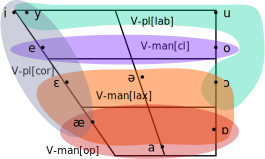
\includegraphics[width=.7\textwidth]{graphics/vowelcharts/bothoa-oral-vowels-features}
  \caption{Featural classes of vowels in in Bothoa Breton}
  \label{fig:natural-classes-bothoa}
\end{figure}


\subsubsection{Stress-related alternations}
\label{sec:stress-relat-altern}

As described above in \cref{sec:stress}, stress mostly stays immobile within a paradigm or across morphologically related items, and where it does move, some form of secondary stress very often remains. Nevertheless, a few alternations can be found.

\paragraph{Data}
\label{sec:data}

As described by \citet{humphreys95:_phonol_bothoa_saint_nicol_pelem}, the plural suffixes \suff{ən} and \suff{jən} cause the stress to shift from a short vowel to the vowel preceding the suffix.\footnote{\citet[p.~247]{humphreys95:_phonol_bothoa_saint_nicol_pelem} says that the stress shift happens \enquote{sometimes}; however, his examples of lack of shift are either words with monosyllabic bases (where the shift applies vacuously) or bases with long vowels, where the shift is blocked for phonological reasons.} These plural suffixes are strongly associated with the agentive derivational suffixes \suff{ər} and \suff{ɛːr}. In the case of the former, the stress shift leads to an alternation between \ipa{[ə]} and \ipa{[æ]}, as shown in \cref{ex:schwa-ae-alternation}:

\ex.\label{ex:schwa-ae-alternation}\a.\a.\twe{[maˈsõːnər]}{masoner}{mason}
\b.\twe{[masoˈnærjən]}{masonerion}{masons}
\z.\b.\a.\twe{[ˈtoːər]}{toer}{roofer}
\b.\twe{[toˈærjən]}{toerion}{roofers}
\b.\mbi{[ˈtoːərjən]}

The alternation between \ipa{[æ]} and \ipa{[ə]} also appears in the conditional suffix \suff{æf} discussed above in \cref{sec:trough-pattern}; the hyphens shows morpheme boundaries for clarity:

\ex.\a.\twe{[ma ˈt-æf-æ]}{ma teufe}{[if] [(s)he] came}
\b.\twe{[ma ˈpaːl-əf-æ]}{ma palfe}{[if] [(s)he] dug}

In general, the vowels \ipa{[æ]}, \ipa{[ɒ]}, and \ipa{[a]} in the \enquote{trough} position all can alternate with the schwa. \Cref{ex:low-vowel-reduction} shows this for \ipa{[ɒ]} and \ipa{[a]}:

\ex.\label{ex:low-vowel-reduction}\a.\a.\twe{[ˈlɒɡɒd̥]}{logod}{mice}
\b.\twe{[ˈlɒɡətad̥]}{logota}{catch mice}
\z.\b.\a.\twe{[ˈtɒhad̥]}{toc'had}{ear (of corn, wheat etc.)}
\b.\twe{[ˈtɒhətad̥]}{toc'hata}{gather, harvest}


However, both these examples involve derivational rather than inflectional morphology. If the trough pattern is created by the addition of inflectional suffixes, the low vowels often remain intact, as seen \cref{ex:bothoa-low-vowel-presevation} with the singulative suffix \suff{ən} and plural \suff{əw}.

\ex.\label{ex:bothoa-low-vowel-presevation}\a.\twe{[ˈlɒɡɒdən]}{logodenn}{mouse}
\b.\twe{[ˈɡɒlɒzəw]}{golvizhier}{beaters}
\b.\twe{[ˈdɒrnəræzəw]}{dornerezhoù}{threshings}

In addition, \ipa{[a]} in the trough position can also be preserved in derivational morphology:

\ex.\label{ex:golched}\a.\twe{[ˈbɒlhad̥]}{golc'hed}{duvet}
\b.\twe{[ˈbɒlhadad̥]}{golc'hedad}{duvet contents}

Note, however, that the suffix \suff{ad} in \cref{ex:golched} is the same suffix that we assumed to be affiliated to the word level with reference to stress data (\cref{sec:strat-aspects-both}), whereas the examples with reduction in \cref{ex:low-vowel-reduction} involve categorial changes, which could reasonably be attributed to the stem level. It would thus appear possible that vowel reduction (at least of \ipa{[a]}) is restricted to the stem level. There are not enough data to provide a confident analysis, however.

It is also possible that the mid vowels \ipa{[ɛ]} and \ipa{[ɔ]} are subject to reduction to schwa in at least some positions. There is evidence for this in the case of \ipa{[ɛ]}. Specifically, both \ipa{[ə]} and \ipa{[ɛ]}, when found in the trough position before a \ipa{[j]} derived from \ipa{[l]} via a palatalization process (see \cref{sec:coron-palat}), undergo coalescence with it to surface as \ipa{[i]}, as seen in \cref{ex:mid-e-reduction}

\ex.\label{ex:mid-e-reduction}\a.\a.\twe{[ˈmɒrzəl]}{morzhol}{hammer}
\b.\twe{[ˈmɒrziəw]}{morzholioù}{hammers}
\z.\b.\a.\twe{[ˈr̥asˌtɛl]}{rastell}{rake}
\b.\twe{[ˈr̥astiəw]}{rastelloù}{rakes}

This is perhaps best analysed as involving reduction from \ipa{[ɛ]} to \ipa{[ə]} in the trough position, unifying the behaviour of the two vowels. In addition, \ipa{[ɛ]} is almost never found in the trough otherwise.\footnote{There is one example, \ipa{[ˈtãnɛrɒh]} `softer' (\emph{teneroc'h}), but it appears anomalous, in that the \ipa{[ɛ]} is the product of an otherwise irregular shortening (\ipa{[tãˈnɛːr]} `tender'), so there is clearly some exceptionality involved.}

In fact, neither \ipa{[ɛ]} nor \ipa{[ɔ]} are very frequent in \enquote{weak} positions, \ie positions other than the main stressed syllable and the final syllable, which, as suggested in \cref{sec:evid-from-segm}, are heads of feet. Neither is found in the trough position. While they may appear in other unstressed syllables, it is overwhelmingly either the initial syllable (which might also be a foot head given \citeauthor{humphreys95:_phonol_bothoa_saint_nicol_pelem}'s description of tertiary stress) or in inflected forms with stress shifts (as in \ipa{[dɛˈvɒtɒh]} `more pious', from \ipa{[ˈdɛvɒd̥]} `pious'), where lack of reduction could be cyclic. Thus, it is not inconceivable that at least \ipa{[ɛ]}, and possibly also \ipa{[ɔ]}, might undergo  reduction to \ipa{[ə]} in some positions, though alternation evidence for \ipa{[ɔ]} is lacking.

\paragraph{Analysis}
\label{sec:analysis}

In terms of the featural specifications shown in \cref{tab:inventory-features-bothoa}, reduction of \ipa{[æ]}, \ipa{[ɒ]}, and \ipa{[ɛ]} (and potentially \ipa{[ɔ]}) can be represented as the delinking of a \fea{V-manner}{open} specification in weak positions. In the case of \ipa{[ɒ]}, this creates \ipa{[ə]} directly; in the case of \ipa{[ɒ]}, the expected segment is \{\fea{V-man}{lax},\fea{V-pl}{cor}\}, \ie the vowel \ipa{[ɛ]}, which is also disallowed in this position and further reduces to \ipa{[ə]}. The relevant autosegmental diagrams are shown in \ref{ex:low-vowel-reduction-autoseg}.

\ex.\label{ex:low-vowel-reduction-autoseg}Reduction of \ipa{[æ]} and \ipa{[ɒ]}\\
\begin{tabular}{l@{\hspace{2em}}l}
  a. Reduction of \ipa{/ɒ/} & b. Reduction of \ipa{/æ/} \\
\begin{tikzpicture}[tree]
\node (rt) {\ipa{ɒ $\rightarrow$ ə}}
  child {node {C-manner}
    child {node (vman) {V-manner}
      child {node (lax) {[lax]}}
      child {node (op) {[open]}}}}
  child {node {C-place}
    child {node {V-place}}};
\join{vman}{op} \delink;
\end{tikzpicture}
&
\begin{tikzpicture}[tree]
\node (rt) {\ipa{æ $\rightarrow$ ə}}
  child {node {C-manner}
    child[narrowtree] {node (vman) {V-manner}
      child {node (lax) {[lax]}}
      child {node (op) {[open]}}}}
  child {node {C-place}
    child {node (vpl) {V-place}
      child {node (cor) {[coronal]}}}} ;
\join{vman}{op} \delink;
\join{vpl}{cor} \delink;
\end{tikzpicture}
\end{tabular}

If the mid vowels \ipa{[ɛ]} and \ipa{[ɔ]} also reduce to schwa in weak positions, both reduction processes can be treated as the delinking of the relevant V-place feature (note that \ipa{[ə]} has a V-place node according to the contrastive hierarchy). This is shown in \ref{ex:mid-vowel-reduction}.

\ex.\label{ex:mid-vowel-reduction}Reduction of \ipa{[ɛ]} and \ipa{[ɔ]}\\
\begin{tikzpicture}[tree]
\node (rt) {\ipa{ɛ/ɔ $\rightarrow$ ə}}
  child {node {C-manner}
    child[narrowtree] {node (vman) {V-manner}
      child {node (lax) {[lax]}}}}
  child {node {C-place}
    child {node (vpl) {V-place}
      child {node (cor) {[coronal]/[labial]}}}} ;
\join{vpl}{cor} \delink;
\end{tikzpicture}

In computational terms, this alternations presents a straightforward instance of the reduction of subsegmental complexity in non-head position, in line with other privative approaches such as those of \citet{harris97:_licen_inher,harris05:_vowel_reduction,harris-urua}. I will assume a positional\hyp faithfulness approach \citep[\egm][]{beckman,alderete1999,iosad10:_motiv}, although nothing in particular hinges on this in Breton. The rankings are shown in \ref{breton-reduction-ranking}. The basic idea is that constraints against complex structures (such as *\us{ə, a, i}, which corresponds to *\ipa{[æ]}, and *\us{ə, a}, \ie *\ipa{[ɒ]}) dominate general \textsc{Max} constraints (which effects vowel reduction) but not \textsc{Max}\hd{} constraints, which block reduction in foot heads.

\ex.\label{breton-reduction-ranking}Vowel reduction in Bothoa Breton\\
\wraptbl{\begin{OTmultitableau}{8}\OTdashes{1,2,4,5,7}\OTsolids{3,6}
\OTmtoprow{\textsc{Max}\hd(\us{i}),\textsc{Max}\hd(\us{a}),\textsc{Max}(\us{ə}),*\us{ə, a, i},*us{ə, i},*\us{ə, a},\textsc{Max}(\us{a}),\textsc{Max}(\us{i})}
\OTmcandrow[/toːær/]{[(ˈtoː)ær]}{,,,*!,*,*,,}
\OTmcandrow{[(ˈtoː)ɛr]}{,,,,*!,,*,}
\OTmcandrow{[(ˈtoː)ɒr]}{,,,,,*!,,*}
\OTmcandrow{[(ˈtoː)ar]}{,,*!,,,,,*}
\OTmcandrow{[(ˈtoː)ir]}{,,*!,,,,*,}
\OTmcandrow[][\OThand]{[(ˈtoː)ər]}{,,,,,,*,*}
\OTmcandrow[/toærjən/][\OThand]{[to(ˈærjən)]}{,,,*,*,*,,}
\OTmcandrow{[to(ˈɛrjən)]}{,*!,,,*,,*,}
\OTmcandrow{[to(ˈɒrjən)]}{*!,,,,,*,,*}
\OTmcandrow{[to(ˈarjən)]}{*!,,*,,,,*,*}
\OTmcandrow{[to(ˈirjən)]}{,*!,*,,,,*,}
\OTmcandrow{[to(ˈərjən)]}{*!,*,,,,*,*}
\end{OTmultitableau}
}

I assume that delinking only affects features rather than nodes, because this allows for an analysis where reduction is driven by constraints on feature co\hyp occurrence (\ie *\ipa{[æ]} and the like), meaning that delinking of entire nodes does not lead to harmonic improvement. An alternative analysis is based on constraints that prohibit the combination of certain features with certain nodes. This would mean that, for instance, the two constraints *\ipa{[ɛ]} (specifically *\{\fea{V-man}{lax}, \fea{V-pl}{cor}\}) and *\ipa{[ɔ]} (*\{\fea{V-man}{lax}, \fea{V-pl}{lab}\}) could be replaced by a single constraint *\{\fea{V-man}{lax}, C-pl\}, which would also (partially) subsume *\ipa{[æ]}. Given the relatively meagre evidence for vowel reduction, any decision at this point is more or less arbitrary. From an architectural perspective, since I recognize both nodes and features as possible arguments in markedness constraints, the difference between the approaches is negligible. I assume the precise choice rides on a closer analysis of the data, whereas conceptually the difference is not enormous.\footnote{In this section I assumed that vowel reduction is in fact a phonological process, possibly with lexical or stratal restrictions. There are some indications that it is not necessarily so and that at least in some cases the vowel written \ipa{[ə]} in the trough position might in fact be a phonological \ipa{[æ]}, meaning that the \phonint{ə} is an artefact of phonetic interpretation \citep[\cfm][]{barnes2007,iosad10:_motiv}. The evidence is provided by the fact that there are some examples of the \ipa{[æ]} in the conditional suffix \suff{æf} surfacing in a medial syllable. One example is \ipa{[ˈøːrəʒæfæ]} `([s]he) would marry'. Note that the \ipa{[æ]} is not in the trough position as defined in \cref{sec:trough-pattern}, although the form does alternate with \ipa{[ˈøːrəʒfæ]}. Another example is \ipa{[ˌkusˈkæfæ]} `([s]he) would sleep', which coexists with \ipa{[ˈkuskfæ]}, and note the irregular stress pattern. Both examples are noted for one speaker, and are described as \enquote{sporadic variants} (\foreigntextquote{french}{avec le statut de variantes sporadiques}). The issue can only be resolved by empirical study.}

\subsubsection{Vowel raising}
\label{sec:vowel-raising}

Short unstressed \ipa{[e]} productively alternates with \ipa{[i]} in hiatus (recall that phonetically this \ipa{[i]} may be realized as a non-syllabic glide). This \ipa{[i]} can be preceded by dorsal stops.

\ex.\a.\a.\twe{[ˈalve]}{alc'hwez}{key}
\b.\twe{[ˈalviəw]}{alc'hwezioù}{keys}
\b.\mbp{ˈalvjəw}
\z.\b.\a.\twe{[ˈklɔːɡe]}{kloge}{ladle}
\b.\twe{[ˈklɔːɡiəw]}{klogeoù}{ladles}
\b.\mbp{ˈklɔːɡjəw}
\z.\b.\a.\twe{[ˈʃaːre]}{charre}{scythe handle}
\b.\twe{[ˈʃaːriad̥]}{charread}{forceful blow}
\z.\b.\a.\twe{[ˈbøːre]}{beure}{morning}
\b.\twe{[ˈbøːriɒh]}{beureoc'h}{earlier in the morning}


However the raising is motivated (note that in all cases it happens in the trough position, since an unstressed \ipa{[e]} is in these cases preceded by a stressed syllable and necessarily followed by another syllable), in autosegmental terms it is easily understood as the delinking of a \fea{V-manner}{closed} feature, as seen in \cref{ex:e-raising}.

\ex.\label{ex:e-raising}Raising of \ipa{[e]} via delinking\\
\begin{tikzpicture}[tree]
\node (rt) {\ipa{e $\rightarrow$ i}}
  child {node {C-manner}
    child {node (vman) {V-manner}
      child {node (cl) {[closed]}}}}
  child {node {C-place}
    child {node {V-place}
      child {node {[coronal]}}}} ;
\join{vman}{cl} \delink;
\end{tikzpicture}

Again, in principle this process might be treated as delinking of the manner node rather than of the feature, but this would require a more complicated analysis which would have to account for the lack of similar alternations with \ipa{[o]}. There are indeed no examples of \ipa{[o]} raising to \ipa{[u]} in a similar context, which might be explained by the fact the deleting the manner specification from \ipa{[o]} would result in an otherwise prohibited empty segment. However, any account of the behaviour of \ipa{[o]} would be pure conjecture: there is only one example of \ipa{[o]} in hiatus (\ipa{[toˈærjən]} `roofers'), but \ipa{[o]} is not in the trough position, and in addition it coexists with \ipa{[ˈtoːərjən]}, which makes the status of the form less clear. Thus, for the sake of the argument I will assume that raising is explained by some constraint prohibiting \{\fea{V-man}{cl}, \fea{V-pl}{cor}\} in hiatus dominating \textsc{Max}(\fea{V-man}{cl}) but not \textsc{Max}(\fea{V-pl}{cor}).

\subsubsection{The nasal vowels}
\label{sec:nasal-vowels-1}

I do not discuss the nasal vowels at length in this dissertation. I note two particular properties that would need to be discussed in a fuller account of Bothoa Breton phonology.

\paragraph{Representational issues}
\label{sec:repr-issu}

There is suggestive evidence for treating nasal vowels as representationally related to the coronal nasal \ipa{[n]}. The clearest evidence is provided by alternations such as that shown in \cref{ex:pontiou}

\ex.\label{ex:pontiou}\a.\twe{[ˈpond̥]}{pont}{bridge}
\b.\twe{[ˈpõːʃəw]}{pontioù}{bridges}

Here, the nasal does not appear because of a restriction on homorganic nasal\endash fricative sequences which appears to be exceptionless in Bothoa Breton.\footnote{Non-homorganic sequences are allowed: \ipa{[ˈamzər]} `weather', \ipa{[ˈpinviʧad̥]} `enrich oneself'.} Instead, the nasal coalesces with the preceding vowel. A contrast between \ipa{[Ṽn]} and \ipa{[Vn]} sequences seems to exist, but it is said to be most robust in unstressed position, and it is not immediately clear that unstressed \enquote{nasal vowels} are not really the result of a gesture overlap under conditions of reduced duration. No definitive pronouncements appear possible at this stage.

\paragraph{Length}
\label{sec:length}

According to \citet{humphreys95:_phonol_bothoa_saint_nicol_pelem}, length is not distinctive for nasal vowels in Bothoa Breton except \ipa{[ã]} in the position before \ipa{[n]} (which is also interesting in view of the relationship between nasal vowels and \ipa{[n]} just sketched). This conclusion is based on the rôle of the nasal vowels in lexical contrast, which is indeed restricted. However, nasal vowels do appear to obey restrictions on long vowels, in that unstressed nasal vowels (which, except \ipa{[ã]}, are relatively infrequent) are uniformly short. Since prosody is not necessarily lexically contrastive, the length of nasal vowels might need to be represented in the phonology somehow. Again, I leave this matter aside here.

\subsubsection{Diphthongs}
\label{sec:diphthongs-bothoa}

As discussed in \cref{sec:diphthongs}, the diphthongs of Bothoa Breton are \ipa{[ɛĭ]}, \ipa{[əy̆]}, \ipa{[əw]} and \ipa{[aw]}, and \ipa{[ãw̃]}. Phonologically, their most important characteristic is that they pattern with short rather than long vowels in that they do no necessarily attract stress and that they may precede tautosyllabic consonants.

In \cref{sec:syll-size-restr} I have argued that diphthongs are best represented as a single branching mora. Further, I propose that the mora dominates segments which from a featural perspective are both vowels, just as in Welsh.

The non-nucleus part of the diphthong can only contain mannerless segments (\ie the high vowels). While this is not necessarily significant in view of the typological frequency of such a pattern, it might also be taken as additional evidence for the status of high vowels as mannerless segments, as this restriction receives a straightforward featural basis: no V-manner nodes are allowed in the non-head portion of a diphthong.

As for the nuclear portion, there is evidence for just one contrast in nucleus quality: that of \ipa{[əw]} (which is \phonint{æw} for some speakers) versus \ipa{[aw]}. I suggest that from a phonological perspective the possible diphthongal nuclei are \ipa{[ə]} (\fea{V-manner}{lax}) and \ipa{[a]} (\fea{V-manner}{open}), with no V-place features, or more generally complex segments, allowed in diphthong nuclei.\footnote{The apparent lack of diphthongs with a \ipa{[o]} nucleus has to be admitted as a lexical gap.} If this generalization is correct, it provides some evidence for \ipa{[ə]} and \ipa{[a]} as unit segments for V-manner features. Thus, in the remainder of this chapter I will use the phonological notation for diphthongs as shown in \cref{tab:diphthong-notation-breton}. I use the symbol \ipa{[w]} rather than \ipa{[u]} for the diphthongal glide for consistency with \ipa{[ãw̃]}.

\begin{table}[htp]
  \centering
  \begin{tabular}{*{2}{l}}
    \toprule
    Phonetic notation & Surface phonology \\
    \midrule
    \ipa{[ɛĭ]} & \ipa{[əi]} \\
    \ipa{[əy̆]} & \ipa{[əy]} \\
    \ipa{[əŭ]/[æŭ]} & \ipa{[əw]} \\
    \midrule
    \ipa{[aŭ]} & \ipa{[aw]} \\
    \ipa{[ãŭ̃]} & \ipa{[ãw̃]} \\
    \bottomrule
  \end{tabular}
  \caption{Phonological notation for diphthongs}
  \label{tab:diphthong-notation-breton}
\end{table}


\subsubsection{Morphologically conditioned alternations}
\label{sec:morph-cond-altern}

A number of vowel changes in inflection appear to be driven by morphology or even triggered on a word-by-word basis.

The back vowels \ipa{[a]}, \ipa{[ɔ]} and \ipa{[ã]} are fronted to \ipa{[i]} by the plural suffix \suff{i}, but this suffix is unproductive and extremely rare. Instances for \ipa{[i]} that appear in this formation trigger palatalization of dorsal stops to postalveolar fricatives.

\ex.\a.\a.\twe{[ˈkɔɡ̊]}{kog}{rooster}
\b.\twe{[ˈʧiːdʒi]}{kegi}{roosters}
\z.\b.\a.\twe{[ˈpɔːləz̥]}{polez}{chicken}
\b.\twe{[ˈpiləzi]}{polezi}{chickens}
\z.\b.\a.\twe{[ˈɡast]}{gast}{bitch}
\b.\twe{[ˈdʒisti]}{gisti}{bitches}
\z.\b.\a.\twe{[ˈbrãːn]}{bran}{crow}
\b.\twe{[ˈbriːni]}{brini}{crows}

There is a very small class of nouns forming plurals purely by vowel change, such as \ipa{[ˈmiːn]} `stone' (\emph{maen}), plural \ipa{[ˈməin]} (\emph{mein}); I do not have much to say about these alternations here.

\subsubsection{Summary: vowels}
\label{sec:summary:-vowels}

Despite having a relatively large vowel inventory, Bothoa Breton does not exhibit many vocalic alternations that would give evidence for the representations. The alternation classes I propose for Bothoa Breton are shown in \cref{fig:alt-classes-bothoa}. In addition to the classes discussed in this section, \ipa{[i]} and \ipa{[y]} are grouped together because they trigger a palatalization process, as described below in \cref{sec:palatalization}.
\begin{figure}[htp]
  \centering
  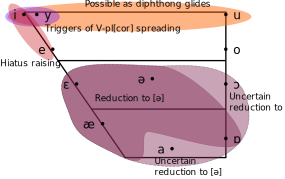
\includegraphics[width=.7\textwidth]{graphics/vowelcharts/bothoa-oral-vowels-classes}
  \caption{Alternation classes in Bothoa Breton}
  \label{fig:alt-classes-bothoa}
\end{figure}


As \cref{fig:alt-classes-bothoa} shows, the evidence for some of the specifications I propose is rather inconclusive; in some cases, as in the case of \ipa{[o]}, the assignment of features has to be relatively arbitrary. However, this system allows us to give an account of such facts as can be gleaned from \posscite[']{humphreys95:_phonol_bothoa_saint_nicol_pelem} description. A fuller account is of course possible, but it requires a better understanding of the possible alternations and their conditioning, as well as of the interaction between prosody and segmental phonology, than is available at the moment

\subsection{Consonant representations and alternations}
\label{sec:cons-altern}


The featural specifications I propose for consonants are given in \cref{tab:bothoa-consonant-features}. To save space, \cref{tab:bothoa-consonant-features} only gives \emph{featural} specifications, whereas empty nodes whose appearance is driven by contrastive specification are discussed in more detail below.

\begin{table}[htp]
  \centering
\resizebox{\textwidth}{!}{
  \begin{tabular}{lccccccccc}
    \toprule
& \multicolumn{2}{c}{C-place} & \multicolumn{2}{c}{V-place} & \multicolumn{2}{c}{C-manner} & \multicolumn{2}{c}{V-manner} & C-laryngeal \\
\cmidrule(r){2-3}
\cmidrule(lr){4-5}
\cmidrule(lr){6-7}\cmidrule(lr){8-9}\cmidrule(l){10-10}
Segment    & [labial]      & [coronal]     & [coronal]     & [labial]      & [open]        & [closed]      & [open]        & [closed]      & [voiceless]   \\
\midrule
\ipa{/p/}  & \checkmark    &               &               &               &               & \checkmark    &               &               & \checkmark    \\
\ipa{/b/}  & \checkmark    &               &               &               &               & \checkmark    &               &               &               \\
\ipa{/t/}  &               & \checkmark    &               &               &               & \checkmark    &               &               & \checkmark    \\
\ipa{/d/}  &               & \checkmark    &               &               &               & \checkmark    &               &               &               \\
\ipa{/k/}  &               &               &               &               &               & \checkmark    &               &               & \checkmark    \\
\ipa{/ɡ/}  &               &               &               &               &               & \checkmark\gc &               &               &               \\
\ipa{/ɡw/} &               &               &               & \checkmark    &               & \checkmark    &               &               &               \\
\midrule
\ipa{/ʧ/}  &               &               & \checkmark    &               &               & \checkmark    &               &               & \checkmark    \\
\ipa{/dʒ/} &               &               & \checkmark    &               &               & \checkmark    &               &               &               \\
\ipa{/dʒɥ/}& \checkmark    &               & \checkmark    &               &               & \checkmark    &               &               &               \\
\midrule
\ipa{/f/}  & \checkmark    &               &               &               &               &               &               &               & \checkmark    \\
\ipa{/v/}  & \checkmark\gc &               &               &               &               &               &               &               &               \\
\ipa{/s/}  &               & \checkmark    &               &               &               &               &               &               & \checkmark    \\
\ipa{/z/}  &               & \checkmark\gc &               &               &               &               &               &               &               \\
\ipa{/ʃ/}  &               & \checkmark    & \checkmark    &               &               &               &               &               & \checkmark    \\
\ipa{/ʒ/}  &               & \checkmark    & \checkmark    &               &               &               &               &               &               \\
\ipa{/h/}  &               &               &               &               &               &               &               &               & \checkmark\gc \\
\midrule
\ipa{/ɥ/}  & \checkmark    &               & \checkmark    &               &               &               &               &               &               \\
\midrule
\ipa{/n/}  &               &               &               &               & \checkmark    &               &               & \checkmark    &               \\
\ipa{/m/}  & \checkmark    &               &               &               & \checkmark    &               &               & \checkmark    &               \\
\ipa{/j̃/}  &               &               & \checkmark    &               & \checkmark    &               &               & \checkmark    &               \\
\ipa{/l/}  &               &               &               &               & \checkmark\gc &               &               &               &               \\
\ipa{/r/}  &               &               &               &               & \checkmark    &               & \checkmark    &               &               \\
\midrule
\ipa{/i/}  &               &               & \checkmark\gc &               &               &               &               &               &               \\
\ipa{/a/}  &               &               &               &               &               &               & \checkmark\gc &               &               \\
\ipa{/o/}  &               &               &               &               &               &               &               & \checkmark\gc &               \\
\ipa{/u/}  &               &               &               & \checkmark\gc &               &               &               &               &               \\
\bottomrule
  \end{tabular}}
  \caption{Featural specifications for consonants in Bothoa Breton}
  \label{tab:bothoa-consonant-features}
\end{table}

Note that, as in the case of Welsh, I associate contrastive non-specification for a feature with the presence of a bare featural node. An important feature of Bothoa Breton, as I argue below, is that it makes use of the possibility of ternary contrasts (presence of a feature \vs presence of a bare node \vs absence of a feature) in surface phonological representations.

In this section I consider palatalization, high vowel gliding, and word-level laryngeal phonology, before moving on to initial mutations.

\subsubsection{Palatalization}
\label{sec:palatalization}

I discuss two kind of palatalization separately: the palatalization of dorsals by high front vowels and the palatalization of coronals and dorsals due to coalescence with an onset \ipa{[i]}.

\paragraph{Velar palatalization}
\label{sec:velar-palatalization}

The postalveolar affricates \ipa{[ʧ]} and \ipa{[dʒ]} appear in many contexts where there is no evidence for deriving them from other segments: they contrast with dorsal stops, fail to alternate with them, and the context is not \emph{a priori} conducive to palatalization. This is shown in \cref{ex:postalveolar-contrasts}.

\ex.\label{ex:postalveolar-contrasts}\a.\a.\twe{[ˈsʧøːl]}{skeul}{ladder}
\b.\twe{[ˈkəwəd̥]}{kavout}{find}
\z.\b.\a.\twe{[ˈʧɛvələɡ̊]}{kefeleg}{woodcock}
\b.\twe{[kazəˈkɛnəɡ̊]}{kazekenned}{mares}
\z.\b.\a.\twe{[ˈʧahəd̥]}{kerzhet}{to walk}
\b.\twe{[ˈkaləd̥]}{kalet}{hard}

This would seem to demonstrate that \ipa{[ʧ]} and \ipa{[dʒ]} are part of the inventory of underlying segments. I suggest this is indeed the case. Nevertheless, there is also evidence that at least some instances of \ipa{[ʧ]} and \ipa{[dʒ]} are derived from dorsal stops.

\subparagraph{Data}
\label{sec:data-1}

First, sequences of dorsal stops \ipa{[k~ɡ]} (phonetically \phonint{kʲ~ɡʲ} in this position) followed by high front vowels \ipa{[i~y]} are relatively rare in the language. The sequence \ipa{[ky]} appears not to be found at all, while \ipa{[ɡy]} is only attested in the clearly borrowed name \ipa{[ɔɡysˈtiːn]} `Augustine' (in addition, it is found in an underived form, which are known to sustain exceptions). As for \ipa{[ki]} and \ipa{[ɡi]}, they are found in the following contexts:

\begin{itemize*}
\item Postlexically:
\end{itemize*}

\ex.\a.\twe{[ak i ˈziː]}{hag he zi}{and her house}
\b.\twe{[aɡ ˈivul]}{hag eoul}{and oil}

\begin{itemize*}
\item Before the future suffixes \suff{id̥} (2nd person plural), \suff{iːãmp} (1st person plural), \suff{iːaj̃\kern-1pt ʧ} (2rd person plural):
\end{itemize*}

\ex.\a.\twe{[ˈlakiãmb̥]}{lakiamp}{we will put}
\b.\twe{[ˈpleːɡid̥]}{plegit}{you (pl.) will fold}

\begin{itemize*}
  \item Before certain derivational suffixes:\footnote{There are also exists a derivational suffix \suff{yz̥}, but there appear to be no relevant examples.}
\end{itemize*}

\ex.\a.\twe{[ˈvrãŋkiz̥]}{frankiz}{open space, the outdoors}
\b.\twe{[ˈbeɡiʃad̥]}{begisat}{to chatter}

\begin{itemize*}
  \item Before instances of \ipa{[i]} derived by raising (\cref{sec:vowel-raising}):
\end{itemize*}

\ex.\a.[]\twe{[ˈklɒːɡiəw]}{klogeoù}{ladles}


Alternations between dorsal stops as such and the affricates are few and far between. They are found with the plural suffix \suff{i}, which also causes the otherwise irregular overwriting of the root vowel with an \ipa{[i(ː)]}. This high vowel in the root also causes the alternation.\footnote{There is also at least one instance of velar palatalization in an irregular plural before a non-high front vowel: \ipa{[dʒɛvər]} `goats' (\emph{gevr}), \cf singular \ipa{[ˈɡawr]}.}

\ex.\a.\a.\twe{[ˈkɔɡ̊]}{kog}{rooster}
\b.\twe{[ˈʧiːdʒi]}{kegi}{roosters}
\z.\b.\a.\twe{[ˈɡast]}{gast}{bitch}
\b.\twe{[ˈdʒisti]}{gisti}{bitches}

I suggest that the fact that \ipa{[k]} and \ipa{[ɡ]} are all but excluded from the position before high front vowels morpheme-internally indicates that the phonological computation maps the dorsal stops to \ipa{[ʧ]} and \ipa{[dʒ]} in this context. I will refer to this alternation as velar palatalization. It happens only at the stem level, explaining the paucity of alternations, as well as the fact that the alternation is blocked before \ipa{[i]} derived by raising; in \cref{sec:gliding} below I argue that raising is a word-level process, which explains the counterfeeding relationship. It is noteworthy that clearly inflectional suffixes such as the future morphemes do not trigger velar palatalization, since inflection is normally assumed to happen only at the word level.\footnote{\label{fn:kegi-stratal}Note, however, that the inflectional suffix \suff{i} also appears to trigger this alternation in \ipa{[ˈʧiːdʒi]} `roosters', from \ipa{[ˈkɔɡ̊]}. Following \citet{bermudez-oterong}, I suggest that this form is an irregular root-based formation rather than one where the inflectional suffix is added to the stem, as demonstrated by the fact that the root allomorph \ipa{[ˈʧiːdʒ]} is bound, and root\hyp based formations undergo stem\hyp level phonology. See also below \cref{sec:front-unro-vowel} for more discussion.}

Moreover, at least in the case of \ipa{[ʧ]} there is evidence from initial consonant mutations that some tokens of word-initial affricates are derived from underlying dorsal stops followed by \ipa{[j]}. Specifically, the so-called spirantization (see below \cref{sec:spirantization}) involves a change from \ipa{[k]} to \ipa{[h]}. Moreover, when the \ipa{[k]} precedes a sonorant, the result is the so-called voiceless sonorant (as discussed below in \cref{sec:spirantization}, this is important evidence for representing voiceless sonorants as \ipa{[h]}\endash sonorant sequences). This is shown in \cref{ex:k-spirantization}.

\ex.\label{ex:k-spirantization}\a.\a.\twe{[ˈkaːz̥]}{kazh}{cat}
\b.\twe{[mə ˈhaːz̥]}{ma c'hazh}{my cat}
\z.\b.\a.\twe{[ˈkriːb̥]}{krib}{comb}
\b.\twe{[mə ˈhriːb̥]}{ma c'hrib}{my comb}

The outcome of the spirantization of \ipa{[ʧ]} in the sequence \ipa{[ʧɥ]} is the same as that of \ipa{[k]} before sonorants

\ex.\a.\twe{[ˈʧɥiːzin]}{kegin}{kitchen}
\b.\twe{[i hɥiːzin]}{he c'hegin}{her kitchen}


This behaviour is consistent with the word for `kitchen' being underlyingly represented as \ipa{/kɥiːzin/}.

Similarly, \ipa{[ʧ]} before a high front vowel is spirantized to \ipa{[h]}, which could potentially be derived if the \ipa{[ʧ]} corresponded to \ipa{/k/}:

\ex.\a.\twe{[ˈʧiː]}{ki}{dog}
\b.\twe{[ə ˈhiː]}{ar c'hi}{the dog}

No such argument from mutation can be made for \ipa{[dʒ]}. If words such as \ipa{[dʒiːr]} `word' (\emph{ger}) had an underlying dorsal stop, we would expect that stop to become \ipa{[h]} in the course of lenition (\cref{sec:lenition}). However, this does not happen, and \ipa{[dʒ]} remains unchanged:

\ex.\label{ex:no-dz-as-g}\a.\a.\twe{[ˈɡɔˌdɛl]}{godell}{pocket}
\b.\twe{[i ˈhɔˌdɛl]}{e c'hodell}{his pocket}
\z.\b.\a.\twe{[ˈdʒiːr]}{ger}{word}
\b.\twe{[i ˈdʒiːr]}{e c'her}{his word}
\b.*\mbi{[i ˈhiːr]}

There is thus very little evidence for underlying \ipa{/ɡi/} sequences which surface as \ipa{[dʒi]}, even though there is circumstantial evidence for a \ipa{/ɡ/}$\rightarrow$\ipa{/dʒ/} change before high front vowels in forms such as \ipa{[ˈdʒisti]} (as the plural of \ipa{[ˈɡast]}).\footnote{\label{fn:article-allomorphy}\citet{humphreys95:_phonol_bothoa_saint_nicol_pelem} discusses another type of evidence for a distinction between underived \ipa{[ʧ~dʒ]} and derived ones. Briefly, Bothoa Breton distinguishes between two allomorphs of the definite and indefinite articles, which are sensitive to the phonology of the following word. Of particular interest here is the distinction between following coronals and non-coronals: \ipa{[ən ˈdɒrz̥]} `the bread roll' (\emph{an dorzh}) but \ipa{[ə ˈɡəw]} `the lie' (\emph{ar gaou}). In the case of \ipa{[ʧ]} and \ipa{[dʒ]}, the article allomorphy reproduces the diachronic origin: \ipa{[n]}-ful forms are chosen before affricates descending from *\emph{tj} and *\emph{dj} (\ipa{[ən ˈdʒəwl]} `the devil', \cf Welsh \emph{diawl}) but \ipa{[n]}-less forms are used before those going back to dorsals (\ipa{[ə ˈdʒiːr]} `the word', \cf Welsh \emph{gair}). Similarly, underlying initial \ipa{[h]} is associated with \ipa{[n]}-ful forms (\ipa{[ən ˈhãw̃n]} `the name') but \ipa{[h]} derived from \ipa{[ʧ]} (and ultimately \ipa{[k]}) takes \ipa{[n]}-less forms like dorsals (\ipa{[ə ˈhiː]} `the dog', \cf Welsh \emph{cî}). However, I suggest that the article allomorphy cannot be used to diagnose the phonological make-up of following words. First, it is also sensitive to etymological differences that are not recoverable from synchronic alternations, as in the case of initial \ipa{[hw]} (\ipa{[n]}-ful forms before \emph{*huV} and \ipa{[n]}-less forms before *\emph{\ipa{χw}}), so at least some arbitrary subcategorization must be involved (note that I assume \ipa{[w]} and \ipa{[u]} are not phonologically distinct in Bothoa Breton). Second, the class of onsets selecting for \ipa{[n]}-ful forms (\ipa{[t~d~$\emptyset$~h~w]}) does not seem to be motivated by the featural structure of the language otherwise. Finally, if the selection of the article allomorphs were driven by the phonology, it would have to be sensitive to the featural make-up of the initial consonant \emph{before} the application of the palatalization rule. However, palatalization is a stem-level rule, whereas the article is clearly a separate lexical item: this creates an ordering paradox, since one would expect insertion of the article to follow the entire cycle of the phonological derivation in the noun. While this may appear less of an issue in fully parallel frameworks, one would still have to deploy whatever machinery one uses to deal with counterbleeding opacity in this case. Moreover, this example demonstrates the greater restrictiveness of stratal models: while fully parallel frameworks and some current versions of serial OT allow the interaction of any two processes (\eg via \textsc{Prec} constraints in the case of the latter), stratal models impose more restrictive global conditions on rule ordering (\citealp[\cf][]{kiparsky11:_chain} on this point), and they predict such an interaction to be impossible.} I conclude that a process of velar palatalization is active at the stem level in Bothoa Breton, producing \ipa{[ʧ]} and \ipa{[dʒ]} from \ipa{[k]} and \ipa{[ɡ]} before \ipa{[i~y]} (the absence of the opaque mutation pattern of \cref{ex:no-dz-as-g} is accounted for in \cref{sec:lexic-insert-strat}).

\subparagraph{Analysis}
\label{sec:analysis-1}

In featural terms, velar palatalization is represented as a straightforward process of the spreading of \fea{V-pl}{coronal} from \ipa{[i]} and \ipa{[y]} to the placeless dorsal stops. This is shown in \cref{ex:velar-analysis}.

\ex.\label{ex:velar-analysis}Velar palatalization: \ipa{/ki/} $\rightarrow$ \ipa{[ʧi]}\\
\begin{tikzpicture}[tree]
  \node (k) {\ipa{k $\rightarrow$ ʧ}}
  child {node {C-manner}
    child {node {[closed]}}}
  child {node {C-laryngeal}
    child {node {[voiceless]}}} ;
  \node[right=8em of k] (i) {\ipa{i}}
  child {node (cpl) {C-place}
    child {node {V-place}
      child {node {[coronal]}}}} ;
  \join[draw,dashed]{k}{cpl} ;
\end{tikzpicture}


The process of velar palatalization thus provides evidence both for the featural specification of \ipa{[i]} and \ipa{[y]} as \fea{V-place}{coronal} vowels and the markedness relationships and place specifications for the nonanterior stops. Such relationships, with dorsals unmarked for place and easily susceptible to place changes, are of course not uncommon, as documented by \citet[\eg][]{rice96:_defaul_variab,rice03:_featur}.

There are two further remarks that must be made here. First, I assume that spreading is triggered only by \ipa{[i]} and \ipa{[y]} that are parsed as nuclei; see the next section for discussion of onset \ipa{[i]} and \ipa{[y]}. Second, note that spreading is triggered only by those \fea{V-place}{coronal} vowels that do not bear any V-manner features. I suggest that both these restrictions can be expressed as restrictions on domain heads \citep{kenstowicz1997,moren01:_distin,delacy2002,lacy04:_marked_optim_theor,delacy2006,jurgec10:_featur_spread}.

In OT terms, this requires that some constraint driving spreading dominate \textsc{DepLink}(\fea{V-pl}{cor}), although it is dominated by constraints on domain heads. In this instance, we require the following constraints, using the notation \dtei{F} to mean \enquote{head (or \enquote{designated terminal element}) of the domain of [F]} (Following \citealt{jurgec10:_featur_spread}, I assume that \dte-constraints only apply to heads of branching domains, \ie that they are not the same as feature co-occurrence restrictions or moraic enhancement constraints.)

\ex.*\dtei{\fea{V-pl}{cor}}\fea{V-man}{lax}/[cl]: \enquote{assign a violation mark for each head of a \fea{V-pl}{cor} domain that also bears a \fea{V-man}{lax}/\fea{V-man}{cl} feature}.\footnote{It is not enough to ban the presence of a V-manner node with the feature set proposed in \cref{fig:bothoa-contrastive-hierarchy}, because \ipa{[i]} and/or \ipa{[y]} always have to be specified for V-manner to distinguish them from other \fea{V-pl}{cor} segments.}

\ex.\textsc{Have}-\mo/\dtei{\fea{V-pl}{cor}}: \enquote{assign a violation mark for each head of a branching \fea{V-pl}{cor} domain that does not also head a moraic domain}. This constraint ensures that spreading of \fea{V-pl}{cor} only happens from nuclear positions.

As in \cref{cha:pembrokeshire-welsh}, I use the non-committal constraint schema \textsc{Share} to drive spreading. The ranking is shown in \ref{ki-kezek-kloge}, using \ipa{[ˈʧiː]} `dog' to demonstrate palatalization and \ipa{[ˈklɒːɡe]} `ladle' to show lack of spreading from complex segments. I also show the result for an underlying \ipa{/kiɛzeɡ/} `horses', where, under the ranking given in \cref{ki-kezek-kloge}, palatalization fails because the high front vowel is parsed as an onset, so the output at the stem level is \ipa{[kjɛzəɡ]}. This form ultimately surfaces as \ipa{[ˈʧɛzəɡ̊]}, as discussed in \cref{sec:coron-palat} and \cref{sec:gliding}.  To save space, I do not show the constraint \textsc{Max}(\fea{V-man}{cl}) which ensures that this feature is not deleted to satisfy *\dtei{\us{i}}/\fea{V-man}{lax}, as in \ipa{[ˈklɒːdʒi]} for \ipa{/klɒːɡe/}. More nuanced description of the constraint \textsc{Uniformity} also follows below (\cpageref{sec:stem-level} \emph{sqq.}).

\ex.\label{ki-kezek-kloge}Velar palatalization\\
\wraptbl{\begin{OTmultitableau}{7}\OTdashes{1,2,3,6}\OTsolids{4,5}
\OTmtoprow{\textsc{Uniformity},\textsc{Have}-\mo/\dtei{\us{i}},*\dtei{\us{i}}\us{o, ə},\textsc{Onset},\textsc{Share}(\us{i}),\textsc{DepLink}(\us{i}),\textsc{*ComplexOnset}}
\OTmcandrow[/ki/]{[k\fd{iː\smo\smo}{i}]}{,,,,*!,,}
\OTmcandrow[][\OThand]{[\fd{ʧiː\smo\smo}{i}]}{,,,,,*,}
\OTmcandrow[/klɒːɡe/][\OThand]{[ˈklɒːɡ\fd{e\smo}{i}]}{,,,,*,,}
\OTmcandrow{[ˈklɒː\fd{dʒe\smo}{i}]}{,,*!,,,*,}
\OTmcandrow[/kiɛzəɡ/]{[k\fd{i\smo}{i}.ɛ\smo{}zəɡ]}{,,,*!,*,,}
\OTmcandrow{[\fd{ʧi\smo}{i}.ɛ\smo{}zəɡ]}{,,,*!,,*,}
\OTmcandrow[][\OThand]{[k\fd{j}{i}ɛ\smo{}zəɡ]}{,,,,*,,*}
\OTmcandrow{[\fd{ʧj}{i}ɛ\smo{}zəɡ]}{,*!,,,,*,*}
\OTmcandrow{[\fd{ʧ}{i}ɛ\smo{}zəɡ]}{*!,,,,,,}
\end{OTmultitableau}
}

\paragraph{Coronal palatalization}
\label{sec:coron-palat}

The process that I call coronal palatalization, or \enquote{coalescence}, is triggered by certain suffixes.

\subparagraph{Data}
\label{sec:data-7}

In the case of coronal obstruents, coalescence produces postalveolar fricatives \ipa{[ʃ]} and \ipa{[ʒ]}, except in the case of the sequence \ipa{[st]}, in which case the outcome is \ipa{[sʧ]}. The following examples show the alternations:

\ex.\ipa{[d]} $\rightarrow$ \ipa{[ʒ]}
\a.\a.\twe{[ˈpraːd̥]}{prad}{prayer}
\b.\twe{[ˈpraːʒəw]}{pradoù}{prayers}
\z.\b.\a.\twe{[ˈøːrəd̥]}{eured}{marriage}
\b.\twe{[ˈəːrəʒo]}{eurediñ}{marry}

\ex.\ipa{[t]} $\rightarrow$ \ipa{ʃ}
\a.\a.[]\twe{[ˈpond̥]}{pont}{bridge}
\z.\b.\a.[]\twe{[ˈpõːʃəw]}{pontioù}{bridges}

\ex.\ipa{/z/} $\rightarrow$ \ipa{[ʒ]}
\a.\a.\twe{[ˈmiːz̥]}{miz}{month}
\b.\twe{[ˈmiːʒəw]}{mizioù}{months}
\z.\b.\a.\twe{[ˈtemz̥]}{temz}{manure}
\b.\twe{[ˈtemʒo]}{temzañ}{fertilize with manure}

\ex.\ipa{[s]} $\rightarrow$ \ipa{[ʃ]}
\a.\a.[]\twe{[ˈplaz̥]}{plas}{place}
\z.\b.\a.[]\twe{[ˈplaʃəw]}{plasoù}{places}

\ex.\ipa{[st]} $\rightarrow$ \ipa{[sʧ]}
\a.\a.[]\twe{[ˈlɒst]}{lost}{tail}
\b.[]\label{lostou}\twe{[ˈlɒsʧəw]}{lostoù}{tails}

\ex.\ipa{[n]} $\rightarrow$ \ipa{/j̃\kern-1pt/} (phonetically \phonint{ɲ} or \phonint{j̃\kern-1pt})
\a.\a.\twe{[ˈpwiːn]}{poan}{pain}
\b.\twp{ˈpwiːj̃\kern-1pt əw}{poanioù}{pains}
\z.\b.\a.\twe{[ˈʧærn]}{korn}{horn}
\b.\twp{ˈʧærɲəw}{kornioù}{horns}

\ex.\ipa{[l]} $\rightarrow$ \ipa{[j]}
\a.\a.[]\twe{[ˈpaːl]}{pal}{shovel}
\z.\b.\a.[]\twe{[ˈpaːjəw]}{palioù}{shovels}

\ex.\ipa{[ˌɛl]}, \ipa{[əl]} $\rightarrow$ \ipa{[i]}
\a.\a.[]\twe{[ˈmɒrˌzɛl]}{morzhol}{hammer}
\z.\b.\a.[]\twe{[ˈmɒrziəw]}{morzholioù}{hammers}


I interpret this phenomenon as involving coalescence with an onset \ipa{[i]}. That at least some relevant suffixes do contain this segment in their segmental representations is demonstrated by the examples in \ref{ex:broiou-feurmiou}

\ex.\label{ex:broiou-feurmiou}The plural suffixes \suff{iəw} and \suff{iən}
\a.\a.\twe{[ˈbroː]}{bro}{country}
\b.\twe{[ˈbrojəw]}{broioù}{countries}
\z.\b.\a.\twe{[ˈlɛvər]}{levr}{book}
\b.\twe{[ˈlɛvərjəw]}{levrioù}{books}
\z.\b.\a.\twe{[ˈɛskɔb̥]}{eskob}{bishop}
\b.\twe{[ɛsˈkɔbjən]}{eskibien}{bishops}

\ex.\label{ex:otoiad-keriad}The derivational suffix \suff{iad}
\a.\a.\twe{[ɔˈtɔː]}{oto}{car}
\b.\twe{[ɔˈtɔjad̥]}{otoiad}{contents of a car}
\z.\b.\a.\twe{[ˈlwɛːr]}{loar}{moon}
\b.\twe{[ˈlwɛːrjad̥]}{loariad}{lunar month}

Importantly, the explicit \ipa{[j]} appears following exactly those segments that do not undergo coronal palatalization, \ie vowels, labials, and \ipa{[r]}.

As for dorsals before onset \ipa{[i]}, the evidence is somewhat ambiguous. Historically, *\emph{kj} tended to give \emph{ʃ} and *\emph{gj} could yield either \emph{ʒ} or \emph{j} \citep[§585]{histbreton}. In the case of \emph{kj~gj}\,$\rightarrow$\,\emph{ʃ~ʒ}, the treatment is identical to that of coronal stops, although not in the case of *\emph{gj}\,$\rightarrow$\emph{j}.

Examples with suffixation are not abundant, but it is at least possible for sequences of a dorsal stop and \ipa{[j]} to coalesce into affricates:

\ex.\label{elastique}\a.\twe{[ˌlasˈtikən]}{}{rubber band (French \emph{\textfrench{élastique}})}
\b.\twe{[ˈlastiʧəw]}{}{rubber bands}

There is also some evidence for palatalization\hyp as\hyp spirantization in Bothoa Breton from initial mutations. As discussed above in \cref{sec:velar-palatalization}, initial \ipa{[ʧ]} derived from \ipa{[k]} undergoes spirantization to \ipa{[h]}. However, initial \ipa{[ʧ]} before vowels other than \ipa{[i~y]}, \ie in positions where it cannot be derived from \ipa{/k/}, spirantizes to \phonint{ç}, phonologically \ipa{[hj]} (see below \cref{sec:spirantization}), as seen in \cref{chezeg}.

\ex.\label{chezeg}\a.\twe{[ˈʧɛzəɡ̊]}{kazegennoù}{horses}
\b.\twe{[mə ˈhjɛzəɡ̊]}{ma c'hazegennoù}{my horses}

This can be explained if the underlying form of the word is \ipa{/kiɛzəɡ/}, and \ipa{[k]} coalesces with the \ipa{[i]} to create \ipa{[ʧ]}; \cf the tableau in \ref{ki-kezek-kloge}.

The evidence for the treatment of \ipa{/ɡj/} as \ipa{[j]} is sparse, but it is seen in the following example:

\ex.\a.\twe{[ˈbɛːləɡ̊]}{beleg}{priest}
\b.\twe{[ˈbɛːliən]}{belegion}{priests}

As discussed in \cref{sec:front-unro-vowel}, \ipa{[ˈbɛːliən]} can be derived from an intermediate \ipa{[ˈbɛːləiən]} in line with the second treatment.\footnote{There are several examples of this paradigm in Middle Breton \citep{LlydawegCanol,schrijver11:_middl_early_moder_breton}: \emph{b(a)elec} `priest', plural \emph{baeleyen}, \emph{beleien} (but also \emph{beleguyen} with \ipa{[ɡj]}); \emph{marchec} `horse rider', plural \emph{mareien}; \emph{benhuec} `tool', plural \emph{binhuyou}; \emph{guynieyer} `vineyards', Modern Breton \emph{gwinieg}. \citet[§54]{favereau01} notes: \textquote{Words in \emph{--eg} [\ldots] have a slightly irregular plural  in \emph{--eien} or \emph{--eion} (although local usage has sometimes preserved \emph{--egion} [in Vannetais], or \emph{--ejen} [\ie with \ipa{[ʒ]}]~$\leftarrow$ \emph{--egien})} (\foreigntextquote{french}{Les mots en \emph{--eg} [\ldots] ont un pluriel légèrement irregulier en \emph{--eien} ou \emph{--eion} (mais l'usage local a parfois conservé \emph{--egion} W ou \emph{--ejen}~$\leftarrow$ \emph{--egien})}). He also notes doublets such as \emph{kregier} or \emph{krejer} for `fangs' (\emph{krog}), \emph{ste(g)ier} or \emph{stejer} for `strings' (\emph{stag}).} Nevertheless, it appears this pattern is not very regular in Bothoa Breton, so I will assume it is an exception from a synchronic perspective. A possible argument in favour of this assumption is the fact that coalescence as seen in \cref{elastique} applies to what is clearly a recent borrowing, whereas the mapping from \ipa{/ɡj/} to  \ipa{[j]} is necessarily an older process which may have already lost its productivity.

The initial \ipa{[i]} of a suffix, whether part of the suffix itself or produced by palatalization from \ipa{[l]}, can create the variable palatalization phenomena discussed above (p.~\pageref{bothoa-phonetic-palatalization}):

\ex.\label{bordiou-rastelliou}\a.\a.\twe{[ˈbɒrd̥]}{bord}{side}
\b.\twp{ˈbɒrdʒəw}{bordoù}{sides}
\b.\mbp{ˈbɒrdiəw}
\z.\b.\a.\twe{[ˈhrasˌtɛl]}{rastell}{rake}
\b.\twp{ˈr̥astiəw}{rastelloù}{rakes}
\b.\mbp{ˈr̥astjəw}
\b.\mbp{ˈr̥asʧəw}

These changes represent various points on the continuum between almost complete gesture overlap producing a affricate to almost complete dissociation producing a separate vocalic segment (\cf \citealp{zsiga95:_americ_englis,zsiga00:_phonet}). I suggest that they are outside the purview of phonological computation and the correct surface\hyp phonological representations for the words in \cref{bordiou-rastelliou} are \ipa{[ˈbɒrdiəw]} and \ipa{[ˈhrastiəw]}. I return to the question of why these instances of \ipa{[i]} fail to trigger palatalization below in \cref{sec:gliding}.

\subparagraph{Analysis}
\label{sec:analysis-2}

The analysis of coalescence with coronal obstruents does not present significant complications. Coronal stops (\emph{modulo} laryngeal features) are specified as \{\fea{C-manner}{closed}, \fea{C-place}{coronal}\}, while the outcome of palatalization, \ie the fricatives \ipa{[ʃ]} and \ipa{[ʒ]}, is \{\fea{C-place}{coronal},\fea{V-place}{coronal}\}. Simple merger of coronal stops with the \{\fea{V-place}{coronal}\} segment is impossible due to feature co-occurrence constraints, and the C-manner specification is sacrificed to satisfy these latter, as shown in \ref{corpal-scheme}. Since in all cases of coalescence the sequence is followed by a vowel, I assume that coalescence is driven by the combined power of \textsc{Onset} and *\textsc{ComplexOnset} (recall from \ref{ki-kezek-kloge} that the former dominates the latter).

\ex.\label{corpal-scheme}Coronal palatalization: \ipa{/dj/} $\rightarrow$ \ipa{[ʒ]}\\
\begin{tikzpicture}[narrowtree]
\node (d) {\ipa{d$_{1}$}}
  child {node (cman1) {C-man}
    child {node {[cl]}}}
  child {node (cpl1) {C-pl}
    child {node {[cor]}}} ;
\node (j) [right=8em of d] {\ipa{i}$_{2}$}
  child {node {C-pl}
    child {node (vpl1) {V-pl}
      child {node {[cor]}}}} ;
\node[right=8em of j] (z) {\ipa{ʒ$_{1,2}$}}
  child {node (cman2) {C-man$_{1}$1}
    child {node {[cl]}}}
  child {node {C-pl}
    child [missing] {}
    child {node {V-pl}
      child {node {[cor]$_{1}$}}}
    child {node {[cor]$_{2}$}}} ;
\join{z}{cman2} \delink ;
\midwayarrow{j}{z} ;
\end{tikzpicture}

In the case of the coronal fricatives, the situation is all but identical: the only difference is that they do not have a C-manner feature to begin with, so there is simply full coalescence.

The sequence \ipa{[st]} presents a somewhat different outcome,\footnote{Since there are no \ipa{[zd]} sequences, the result for them is unknown.} but one that is straightforwardly predicted by the present proposal. Rather than the expected *\ipa{[sʃ]}, the result of coronal palatalization is \ipa{[sʧ]}. In featural terms, this means that it is the stop's \fea{C-manner}{closed} feature is preserved at the expense of its \fea{C-place}{coronal} specification. The reason for this is presumably a phonotactic constraint against \ipa{[sʃ]} sequences, which are indeed unattested in the language. The derivation is shown in \ref{ex:st-sts}.\footnote{It is also possible that the C-place node also undergoes coalescence, in which case the first segment is phonologically a \ipa{[ʃ]} (recall that phonetically the sequence is realized as \phonint{ɕtɕ}). In any case, there is no contrast between mannerless \{\fea{C-pl}{cor}, \fea{C-lar}{vcl}\} segments before \ipa{[ʧ]}.}

\ex.\label{ex:st-sts}Coronal palatalization: \ipa{/st/} $\rightarrow$ \ipa{[sʧ]}\\
\wraptbl{\begin{tikzpicture}[narrowtree]
\node (s) {\ipa{s$_{1}$}}
  child {node {C-pl}
    child {node {[cor]}}}
  child {node (clar0) {C-lar}
    child {node (vcl0) {[vcl]}}} ;
\node[right=7em of s] (t) {\ipa{t$_{2}$}}
  child {node  {C-lar}
    child {node (vcl1) {[vcl]}}}
  child {node (cman1) {C-man}
    child {node {[cl]}}}
  child {node (cpl1) {C-pl}
    child {node (ccor1) {[cor]}}} ;
\node [right=7em of t] (j) {\ipa{i$_{3}$}}
  child {node {C-pl}
    child {node (vpl1) {V-pl}
      child {node {[cor]}}}} ;
\node[right=7em of j] (s2) {\ipa{s$_{1}$}}
  child {node {C-pl}
    child {node {[cor]}}} ;
\node[right=6em of s2] (ts) {\ipa{ʧ$_{2,3}$}}
  child {node (clar3) {C-lar$_{1,2}$}
    child {node (vcl2) {[vcl]$_{1,2}$}}}
  child {node (cman3) {C-man}
    child {node {[cl]}}}
  child {node {C-pl}
    child {node {V-pl}
      child {node {[cor]}}}} ;
\join[draw,dashed]{cpl1}{vpl1} ;
\join{cpl1}{ccor1} \delink ;
\join[draw]{s2}{clar3} ;
\midwayarrow{j}{s2} ;
\end{tikzpicture}}

The combined tableau for coronal obstruents is shown in \ref{pradiou-lostiou-temzan}. Note that *\textsc{ComplexOnset} (and by extension \textsc{Onset}) have to dominate \textsc{Uniformity} in order to produce coalescence. To save space, I do not show candidates which delete the feature \fea{V-place}{coronal}. I also do not show candidates where an input root node does not have a correspondent, assuming unviolated \textsc{Max}(Root).\footnote{Note that in cases where the coalescing sequence is preceded by a short vowel, as in \ipa{[ˈøːrəʒo]} `to get married' from \ipa{/øːrədio/}, *\textsc{ComplexOnset} can be repaired by building a closed syllable: \ipa{[ˈøː.rəd.jo]}. However, as discussed above (see the tableau in \ref{seblant-doublan-tableau}), I assume \textsc{NoCoda} dominates *\textsc{ComplexOnset}, so this candidate is not viable.}

\ex.\label{pradiou-lostiou-temzan}Palatalization of coronal obstruents: \ipa{[ˈpraːʒəw]} `prayers', \ipa{[ˈlɒsʧəw]} `tails', \ipa{[ˈtemʒo]} `to fertilize with manure'\\
\wraptbl{\begin{OTmultitableau}{7}\OTdashes{1,2,5}\OTsolids{3,4,6}
\OTmtoprow{*\us{ɡ,z,i},*\ipa{[sʃ]},\textsc{Onset},\textsc{ComplexOnset},\textsc{Uniformity},\textsc{Max}(\us{z}),\textsc{Max}(\us{ɡ})}
\OTmcandrow[/praːd$_{1}$i$_{2}$əw/]{[ˈpraː.d$_{1}$i$_{2}$.əw]}{,,*!,,,}
\OTmcandrow{[ˈpraː.d$_{1}$j$_{2}$əw]}{,,,*!,,}
\OTmcandrow{[ˈpraː.\us{ɡ,z,i}$_{1,2}$əw]}{*!,,,,*,,}
\OTmcandrow{[ˈpraː.dʒ$_{1,2}$əw]}{,,,,*,*!,}
\OTmcandrow{[ˈpraː.j$_{1,2}$əw]}{,,,,*,*!,*}
\OTmcandrow[][\OThand]{[ˈpraː.ʒ$_{1,2}$əw]}{,,,,*,,*}
\OTmcandrow[/lɒst$_{1}$i$_{2}$əw/]{[ˈlɒs.t$_{1}$i$_{2}$.əw]}{,,*!,,,}
\OTmcandrow{[ˈlɒs.t$_{1}$j$_{2}$əw]}{,,,*!,,}
\OTmcandrow{[ˈlɒs.\us{ɡ,z,i,h}$_{1,2}$əw]}{*!,,,,*,,}
\OTmcandrow[][\OThand]{[ˈlɒs.ʧ$_{1,2}$əw]}{,,,,*,*,}
\OTmcandrow{[ˈlɒs.ʃ$_{1,2}$əw]}{,*!,,,*,,*}
\OTmcandrow{[ˈlɒs.j$_{1,2}$əw]}{,,,,*,*,*!}
\OTmcandrow[/temz$_{1}$i$_{2}$o/]{[ˈtem.z$_{1}$i$_{2}$.o]}{,,*!,,,,}
\OTmcandrow{[ˈtem.z$_{1}$j$_{2}$o]}{,,,*!,,,}
\OTmcandrow[][\OThand]{[tem.ʒ$_{1,2}$o]}{,,,,*,,}
\OTmcandrow{[tem.j$_{1,2}$o]}{,,,,*,*!,}
\end{OTmultitableau}
}


Among the other phonetic coronals, \ipa{/l/} surfaces as \ipa{[j]}, because coalescence results in the delinking of the C-manner node of the \ipa{[l]} due to feature co-occurrence constraints. In the case of \ipa{[n]}, however, coalescence does create a licit segment. This is shown in \ref{ex:sonorant-coronal-pal}.

\ex.\label{ex:sonorant-coronal-pal}Coronal palatalization of sonorants \\
\a.\ipa{/nj/} $\rightarrow$ \ipa{[j̃\kern-1pt]}\\
\begin{tikzpicture}[narrowtree]
  \node (n) {\ipa{n$_{1}$}}
    child {node {C-man}
      child {node {[op]}}
      child {node {V-man}
        child {node {[cl]}}}
      child[missing] {}} ;
  \node[right=6em of n] (j) {\ipa{i$_{2}$}}
    child {node {C-pl}
      child {node {V-pl}
        child {node {[cor]}}}} ;
  \node[right=10em of j] (nj) {\ipa{j̃\kern-1pt$_{1,2}$}}
    child {node {C-man}
      child {node {[op]}}
      child {node {V-man}
        child {node {[cl]}}}
      child[missing] {}}
    child {node {C-pl}
      child {node {V-pl}
        child {node {[cor]}}}};
   \path (j-1) -- (nj-1) node[pos=.5] {$\Rightarrow$};
\end{tikzpicture}
\b.\ipa{/lj/} $\rightarrow$ \ipa{[j]} \\
\begin{tikzpicture}[narrowtree]
  \node (l) {\ipa{l$_{1}$}}
    child {node {C-man}
      child {node {[op]}}} ;
  \node[right=6em of l] (j) {\ipa{i$_{2}$}}
    child {node {C-pl}
      child {node {V-pl}
        child {node {[cor]}}}} ;
  \node[right=8em of j] (j2) {\ipa{i$_{1,2}$}}
    child {node {C-man}
      child {node {[op]}}}
    child {node {C-pl}
      child {node {V-pl}
       child {node {[cor]}}}};
   \join{j2}{j2-1} \delink;
   \path (j-1) -- (j2-1) node[pos=.5] {$\Rightarrow$};
\end{tikzpicture}


The tableaux for coronal sonorants are given in \ref{poaniou-paliou-tableau} and \ref{loariad-tableau}. The interesting constraint in both cases in *\{\fea{C-man}{op}, \fea{V-pl}{cor}\} (abbreviated *\us{l,i}). In the case of \ipa{/lj/} sequences, this constraint is ranked sufficiently high to prevent the appears of an otherwise unattested segment consisting of these features, and the response of the computation is to delete \fea{C-man}{op} to yield an onset \ipa{[i]}.\footnote{In other Breton dialects, the inventory includes the palatal lateral \ipa{[ʎ]}, which is also the outcome of palatalization, \eg at Plougrescant \citep{le78:_le_ploug}. The difference between these dialects and Bothoa Breton is easily derived via reranking of *\{\fea{C-man}{op}, \fea{V-pl}{cor}\} and \textsc{Max}(\fea{C-man}{op}).} In the case of \ipa{/nj/}, however, this constraint is violated, as the outcome of coalescence is the segment \ipa{/j̃\kern-1pt/}, consisting of the features \{\fea{C-man}{op}, \fea{V-man}{cl}, \fea{V-pl}{cor}\} (or \us{l,o,i} in shorthand notation). In this case, deletion of \fea{C-man}{op} is expected to create a licit segment; however, the segment is the vowel \ipa{[e]}. It cannot be parsed either as a nucleus (since this violates \textsc{Onset}) or as an onset (since this parse is completely impossible for this segment in the language), and therefore candidate (c.) is the winner.\footnote{This situation is reminiscent of the analysis of labial epenthesis in Serbian by \citet{moren-serbian} (\cf also \citealt{iosad10:_palatalization} for Russian), where sequences of a labial and floating \fea{V-place}{coronal} surface as \eg\ \ipa{[pʎ]}, despite the fact that \ipa{[ʎ]} in Serbian is also a relatively complex segment, and alternatives with less subsegmental structure are available for epenthesis: for instance, for underlying \ipa{/kap\textsuperscript{i}ɛ/} `(it) drips' (where \textsuperscript{i} is the floating feature) the winning form is \ipa{[ˈkapʎɛ]} with \{\fea{C-man}{cl}, \fea{V-man}{cl}, \fea{V-pl}{cor}\} \ipa{[ʎ]} rather than, say, \{\fea{V-pl}{cor}, \fea{V-man}{cl}\} \ipa{[ɛ]}. The reason, \citet{moren-serbian} suggests, is top-down conditioning of prosodic structure, which treats the candidate \ipa{[kapʎɛ]} as preferable to *\ipa{[kapɛɛ]}.}

\ex.\label{poaniou-paliou-tableau}Coalescence with sonorants: \ipa{[ˈpwiːj̃\kern-1pt əw]} `pains', \ipa{[ˈpaːjəw]} `shovels'\\
\wraptbl{\begin{OTmultitableau}{7}\OTsolids{3,4,5}\OTdashes{1,2,4,6}
\OTmtoprow{\textsc{SylStruc},\textsc{Onset},\textsc{Max}(\us{o}),\textsc{ComplexOnset},*\us{l,i},\textsc{Uniformity},\textsc{Max}(\us{l})}
\OTmcandrow[/ˈpwiːn$_{1}$i$_{2}$əw/]{[ˈpwiː.n$_{1}$i$_{2}$.əw]}{,*!,,,,,}
\OTmcandrow{[ˈpwiː.n$_{1}$j$_{2}$əw]}{,,,*!,,,}
\OTmcandrow[][\OThand]{[ˈpwiː.$_{1}$j̃\kern-1pt$_{2}$əw]}{,,,,*,*,}
\OTmcandrow{[ˈpwiː.e$_{1,2}$.əw]}{,*!,,,,*,*}
\OTmcandrow{[ˈpwiː.e̯$_{1,2}$əw]}{*!,,,,,*,*}
\OTmcandrow{[ˈpwiː.j$_{1,2}$əw]}{,,*!,,,*,*}
\OTmcandrow[/ˈpaːl$_{1}$i$_{2}$əw/]{[ˈpaː.l$_{1}$i$_{2}$.əw]}{,*!,,,,,}
\OTmcandrow{[ˈpaː.l$_{1}$j$_{2}$əw]}{,,,*!,,,}
\OTmcandrow{[ˈpaː.$_{1}$\us{l,i}$_{2}$əw]}{,,,,*!,*,}
\OTmcandrow[][\OThand]{[ˈpaː.j$_{1,2}$əw]}{,,,,,*,*}
\end{OTmultitableau}
}

In the case of \ipa{[r]}, both coalescence and the deletion of \fea{C-man}{op} would lead to the creation of illicit segments containing \{\fea{V-man}{op}, \fea{V-pl}{cor}\}, and faithfulness blocks the deletion of \fea{V-pl}{cor}. Therefore, with all segmental options exhausted, the derivation settles on a violation of *\textsc{ComplexOnset}. Note that the relative ranking of *\{\fea{V-man}{op}, \fea{V-pl}{cor}\} and \textsc{Max} constraints is immaterial here, although the lack of this segment in the surface inventory indicates that the markedness constraint dominates at least one of the \textsc{Max} constraints. Note, however, that *\{\fea{V-man}{op}, \fea{V-pl}{cor}\} must be outranked by a faithfulness constraint protecting larger structures (\cref{sec:compl-struct-faithf}): this is needed for underlying \ipa{/æ/} (\{\fea{V-man}{op}, \fea{V-pl}{cor}, \fea{V-man}{lax}\}) to surface, at least in foot head position, despite containing the offending feature pair. Note also that forms such as \ipa{[ˈlwɛːrjad̥]} clearly contain complex onsets, because the sequence \ipa{[rj]} is preceded by a long vowel.

\ex.\label{loariad-tableau}Coalescence blocked, complex onset results: \ipa{[ˈlwɛːrjad̥]} `lunar month'\\
\wraptbl{\begin{OTtableau}{8}\OTsolids{4,5,6}\OTdashes{1,2,3,7}
\OTtoprow[/lwɛːr$_{1}$i$_{2}$ad/]{*\us{a,i},\textsc{Max}(\us{i}),\textsc{Onset},\textsc{Max}(\us{a}),\textsc{ComplexOnset},*\us{l,i},\textsc{Uniformity},\textsc{Max}(\us{l})}
\OTcandrow{[ˈlwɛː.r$_{1}$i$_{2}$.ad̥]}{,,*!,,,,,}
\OTcandrow[\OThand]{[ˈlwɛː.r$_{1}$j$_{2}$ad̥]}{,,,,*,,,}
\OTcandrow{[ˈlwɛː.\us{l,a,i}$_{1,2}$ad̥]}{*!,,,,,*,*,}
\OTcandrow{[ˈlwɛː.r$_{1,2}$.ad̥]}{,*!,,,,,*,}
\OTcandrow{[ˈlwɛː.\us{a,i}$_{1,2}$ad̥]}{*!,,,,,,*,*}
\OTcandrow{[ˈlwɛː.\us{l,i}$_{1,2}$ad̥]}{,,,*!,,*,}
\OTcandrow{[ˈlwɛː.j$_{1,2}$ad̥]}{,,,*!,,,*,*}
\OTcandrow{[ˈlwɛː.l$_{1,2}$ad̥]}{,*!,,*,,,*,}
\end{OTtableau}
}

All labials (both obstruents and the sonorant \ipa{[m]}) do not undergo coalescence with \ipa{[j]}; the mechanism is similar to that seen in the case of \ipa{[r]}: \textsc{Max}(\fea{C-pl}{lab}) and \textsc{Max}(\fea{V-pl}{cor}) prevent deletion and feature co-occurrence blocks coalescence, ensuring violaton of *\textsc{Complex\hspace{0pt}Onset} (see below tableau \ref{bihan-tableau}). As concerns the placeless stops (phonetic dorsals), the prediction is that they will undergo a process similar to that shown for the stop in \ipa{[st]} sequences and will surface as \ipa{[ʧ]} \emph{resp.\@} \ipa{[dʒ]}, as shown in \ref{ex:velar-iotation}.

\ex.\label{ex:velar-iotation}Coalescence of placeless stops with \ipa{[j]}\\
\begin{tikzpicture}[narrowtree]
\node (k) {\ipa{k$_{1}$}}
  child {node {C-lar}
    child {node {[vcl]}}}
  child {node (cman1) {C-man}
    child {node {[cl]}}}
  child {node {C-pl}
    child {node {V-pl}}};
\node (j) [right=6em of k] {\ipa{i$_{2}$}}
  child {node (cpl) {C-pl}
    child {node (vpl1) {V-pl}
      child {node {[cor]}}}} ;
\node[right=10em of j] (ts) {\ipa{ʧ$_{1,2}$}}
  child {node {C-lar}
    child {node {[vcl]}}}
  child {node {C-man}
    child {node {[cl]}}}
  child {node {C-pl}
    child {node {V-pl}
      child {node {[cor]}}}} ;
\midwayarrow{cpl}{ts-1} ;
\end{tikzpicture}

This is exactly what happens with word-initial \ipa{[ʧ]} before a vowel other than \ipa{[i]} or \ipa{[y]}, as discussed above.

Note, that coalescence requires *\textsc{ComplexOnset} to dominate \textsc{Uniformity}, which is at odds with the ranking established in \ref{ki-kezek-kloge} for dorsal stops. I suggest that reconciling these rankings is best done within a stratal model. In the next section I present a detailed analysis of stratal differences in the behaviour of high vowels and relate these facts to the different types of palatalization.

\subsubsection{Gliding}
\label{sec:gliding}

In this section I consider the status of the glides \ipa{[w~j~ɥ]} and their relationship to the high vowels \ipa{[u~i~y]}. I argue that \ipa{[w]} and \ipa{[j]} can be considered to be non-nuclear realizations of \ipa{[u]} and \ipa{[i]}, whereas \ipa{[ɥ]} is best treated as a separate segment.

\citet[p.~166]{humphreys95:_phonol_bothoa_saint_nicol_pelem} discusses this matter in little detail. He claims that glides and high vowels are in all but complementary distribution in terms of syllable position, with a few exceptions to be discussed below. Moreover, he notes that syllabic pronunciations very occasionally heard for what are normally \ipa{[w]} and \ipa{[j]}, so \phonint{biˈɔ̃ːn} and \phonint{luˈarn} for \ipa{[ˈbjɔ̃ːn]} `fast' (\emph{buan}) and \ipa{[ˈlwarn]} `fox' (\emph{louarn}). However, he does not discuss the phonological evidence at length. In this section I consider the three potential glides in order.

\paragraph{The back rounded vowel}
\label{sec:back-rounded-vowel}

On the surface, \ipa{[w]} and \ipa{[u]} stand in complementary distribution: no instances of short \ipa{[u]} are found prevocalically, and \ipa{[w]} is never found before consonants (with the exception of \ipa{[w]} as the second part of a diphthong, but we have seen in \cref{sec:diphthongs-bothoa} that in fact I assume it to be nuclear) There are, however, no alternations that would confirm the phonological identity of these segments.\footnote{One possible piece of evidence for a distinction between \ipa{[w]} and \ipa{[u]} is the article allomorphy discussed in \cref{fn:article-allomorphy}, but it is argued there that it is irrelevant.} Thus, it seems safe to conclude that \ipa{[w]} and \ipa{[u]} represent the same phonological segment in non-nuclear and nuclear position respectively. This analysis is further buttressed by the proposed analysis of the lenition of \ipa{[ɡw]}, for which see below in \cref{sec:lenition}.

\paragraph{The front unrounded vowel}
\label{sec:front-unro-vowel}

The situation with \ipa{[i]} is more complex, since there is more evidence for a distinction between \ipa{[i]} and \ipa{[j]}, which comes from palatalization processes. Specifically, \ipa{[j]}, but not \ipa{[i]}, triggers coronal palatalization; on the other hand, both trigger velar palatalization (in certain conditions). To disentangle the behaviour of \ipa{[i]} and \ipa{[j]}, we need a closer analysis of the interaction between morphology and phonology.

As discussed there is evidence for at least one level distinction, in that some \ipa{[i]}-initial suffixes fail to trigger velar palatalization, while it is all but exceptionless morpheme-internally. In addition, \ipa{[i]} derived from \ipa{[e]} via raising is also not a spreading trigger. In this section I consider further evidence for phonological levels.\footnote{I thank Ricardo Bermúdez-Otero for discussion of several issues treated in this section.}

\subparagraph{The stem level}
\label{sec:stem-level}

I suggest gliding is in operation at the stem-level. This is seen most clearly in the existence of morpheme-internal sequences of a labial followed by \ipa{[j]}:

\ex.\a.\twe{[ˈbjan]}{bihan}{small}
\b.\twe{[ˈpjɒh]}{peoc'h}{peace}
\b.\twe{[ˈmjãːwal]}{miaoual}{meow}

As discussed in \cref{sec:coron-palat}, this is due to \textsc{Onset} and faithfulness constraints dominating *\textsc{ComplexOnset}. Another dominated constraint is \textsc{Have}-\mo[V] which requires vowels to project a mora. The tableau is shown in \cref{bihan-tableau}.

\ex.\label{bihan-tableau}Gliding at the stem level: \ipa{[ˈbjan]} `small'\\
\begin{OTtableau}{5}\OTdashes{1,2,3}\OTsolids{4}
\OTtoprow[/b$_{1}$i$_{2}$an/]{*\us{v,i},\textsc{Max}(\us{i}),\textsc{Max}(\us{v}),\textsc{Onset},*\textsc{ComplexOnset}}
\OTcandrow{[b$_{1}$i$_{2}$.an]}{,,,*!,}
\OTcandrow[\OThand]{[ˈb$_{1}$j$_{2}$an]}{,,,,*}
\OTcandrow{[ˈ\us{v,ɡ,i}$_{1,2}$an]}{*!,,,,}
\OTcandrow{[ˈb$_{1,2}$an]}{,*!,,,}
\OTcandrow{[ˈdʒ$_{1,2}$an]}{,,*!,,}
\end{OTtableau}

As for sequences of non-labials followed by \ipa{[i]} and a vowel, more discussion of the rôle of \textsc{Uniformity} is in order. In \ref{ki-kezek-kloge}, I assumed that \textsc{Uniformity} is ranked high enough to prevent coalescence, at least in the case of \ipa{/kj/}, where it cannot be blocked by feature co\hyp occurrence as in \ref{bihan-tableau}.

In \cref{sec:velar-palatalization} I assumed without argument that \ipa{/kiV/} sequences (at the stem level) are mapped to \ipa{[kjV]} rather than \ipa{[ʧV]}. The evidence for this comes mainly from initial consonant mutation. Recall that initial \ipa{[ʧ]} before a non-high vowel undergoes spirantization to \ipa{[hj]} (\phonint{ç}), in parallel with single \ipa{/k/} spirantizing to \ipa{[h]}. However, if we assumed that the coalescence of the two onset segments happened at the stem level, we would run into an ordering paradox: unless the mutation-triggering autosegment is also present at the stem level, it cannot rescue the underlying \ipa{[k]} from coalescence and turn it into \ipa{[h]}. Yet the mutation autosegment cannot come in earlier than the word level (if we assume it is an agreement morpheme) or even the phrase level (if it is part of the lexical representation of the trigger).

On the other hand, if coalescence itself happens on a later level (such as the word level, as discussed below), it is possible to analyse the derivation of \ipa{[ʧɛzəɡ̊]} `horse' from \ipa{/kiɛzəɡ/} without running into these problems. Specifically, if \ipa{[i]} is  parsed into the onset at the stem level, we can unify this coalescence with \enquote{coronal palatalization} (both are triggered at the word level by onset \ipa{[i]}) and ensure that the mutation trigger (which is an exponent of an inflectional category, appearing at the word level) is able to \enquote{see} the underlying \ipa{[k]} and turn it into \ipa{[h]}. Thus, assuming that \ipa{[i]}-gliding is operative at the stem level provides us with an account of dorsal\endash\ipa{[j]} coalescence that does not run into ordering issues.

However, the ranking which ensures the lack of coalescence in \ref{ki-kezek-kloge} also predicts the blocking of coalescence following coronals, and it is not obvious that this prediction is borne out. In the absence of alternations, it is difficult to ascertain whether the stem level allows complex onsets consisting of a coronal and \ipa{[i]}. There are a few examples that could be interpreted in this way, but the number of these is not very great. Some examples are given in \ref{ex:underived-gliding-failure}.

\ex.\label{ex:underived-gliding-failure}\a.\label{pasiantaat}\a.\twe{[pasiˈãnto]}{pasiantaat}{wait}
\b.*\mbi{[paˈʃãnto]}
\z.\b.\a.\twe{[komprəˈnasion]}{komprenasion}{understanding}
\b.*\mbi{[komprəˈnaʃon]}

Many of these words appear to be Romance borrowings; in particular, the suffix \suff{sion} is always borrowed in this form, although it is difficult to say whether such words are treated as monomorphemic or derived in Breton. There are a few exceptions to this generalization, but they are always morphologically non-trivial, involving, for instance, what appears to be bound allomorphs:

\ex.\label{ex:anaoudegezh-talvoudegezh}\a.\a.\twe{[haˈnaːo]}{anavout}{to know}
\b.\twe{[ˈhãndiæz̥]}{anaoudegezh}{knowledge}
\z.\b.\a.\twe{[ˈtalo]}{talvout}{to earn}
\b.\twe{[ˈtalfiæz̥]}{talvoudegezh}{value}

In principle, this could be consistent with either hypothesis. We could take the existence of forms such as \ipa{[komprəˈnasion]} and \ipa{[ˈtalfiæz̥]} as evidence for the admissibility of such complex onsets at the stem level in Bothoa Breton, which would allow for uniform behaviour of \ipa{[i]} following all consonants. On the other hand, the relative peripherality of such sequences could be treated as evidence for their exceptional status: stem-level rules (such as coalescence would have to be) are known to sustain lexical exceptions. A third alternative is to assume that forms such as those in \cref{ex:underived-gliding-failure,ex:anaoudegezh-talvoudegezh} are exceptional in that they contain onsetless syllables because the instances of \ipa{[i]} are underlyingly moraic, and this is faithfully reproduced by the stem\hyp level phonology. In this case, we could assume that an input nonmoraic \ipa{[i]} is allowed to coalesce with preceding coronals, explaining the lack of unambiguous examples of complex \ipa{[Cj]} onsets with coronals.\footnote{The key question here is the status of forms such as \emph{komprenasion}: \citet{humphreys95:_phonol_bothoa_saint_nicol_pelem} writes them as <kómprenasjon>, but given that in all cases that \ipa{[i]} is unstressed, the \enquote{gliding} might just be an effect of shortness.}

I would suggest that this last alternative is in fact the most appealing one. However, if coalescence with coronals is a live rule, we have to explain why it is allowed (\dom{*\textsc{Complex\hspace{0pt}Onset}}{\textsc{Uniformity}}) in this context but blocked in the case of \ipa{[kj]} onsets (\dom{\textsc{Uniformity}}{*\textsc{Complex\hspace{0pt}Onset}}). A possible solution is assuming that coalescence with coronals is disallowed not by the general \textsc{Uniformity} constraint but by a local conjunction constraint [*\{\fea{C-man}{cl}, \fea{V-pl}{cor}\}\&\textsc{Uniformity}]\textsubscript{Seg}, which prohibits coalescence from producing \ipa{[ʧ~dʒ]} but not \ipa{[ʃ~ʒ~j̃\kern-1pt~j]}. This is shown in \cref{no-coronal-coalescence}. As the tableau shows, there is one undesirable prediction, in that it is assumed that underlying \ipa{/stiV/} sequences can surface as \ipa{[stjV]}, and such sequences are unattested. Nevertheless, this is a relatively minor overgeneration issue.

\ex.\label{no-coronal-coalescence}Coalescence cannot produce \ipa{[ʧ]}\\
\wraptbl{\begin{OTmultitableau}{4}\OTsolids{2,3}\OTdashes{1}
\OTmtoprow{*\ipa{[sʃ]},[*\us{ɡ,i}\&\textsc{Uniformity}]\textsubscript{Seg},*\textsc{ComplexOnset},\textsc{Uniformity}}
\OTmcandrow[/k$_{1}$i$_{2}$V/][\OThand]{[k$_{1}$j$_{2}$V]}{,,*,}
\OTmcandrow{[ʧ$_{1,2}$V]}{,*!,,*}
\OTmcandrow[/t$_{1}$i$_{2}$V/]{[t$_{1}$j$_{2}$V]}{,,*,}
\OTmcandrow[][\OThand]{[ʃ$_{1,2}$V]}{,,,*}{}
\OTmcandrow[/st$_{1}$i$_{2}$V/][\OThand]{[s.t$_{1}$j$_{2}$V]}{,,*,}
\OTmcandrow{[s.ʃ$_{1,2}$V]}{*!,,,*}{}
\OTmcandrow{[s.ʧ$_{1,2}$V]}{,*!,,*}{}
\end{OTmultitableau}
}


However, given the unclear status of exceptional forms, I leave the ultimate resolution of this issue for future work.

\subparagraph{The word level}
\label{sec:word-level}

At the word level, gliding is also active, and it is supplemented by coalescence. At the same time \enquote{velar} palatalization is switched off at this level. Consider the forms in \cref{ex:word-level-gliding}, where hyphens mark morpheme boundaries.

\ex.\label{ex:word-level-gliding}\a.\a.\twe{/pwiːn-iəw/}{poanioù}{sorrows}
\b.\mbi{[ˈpwiːj̃\kern-1pt əw]}
\z.\b.\a.\twe{/kwæd-iəw/}{koadioù}{forests}
\b.\mbi{[ˈkwæʒəw]}


The stratal model can also explain why \ipa{[i]} derived by raising from \ipa{[e]} fails to be reparsed into the onset, and thus does not participate in coalescence, as seen in forms such as \mbox{\ipa{[ˈklɒːɡiad̥]}} `ladleful' (*\ipa{[ˈklɒːdʒad̥]}), from \ipa{[ˈklɒːɡe]}. At the stem level, the vowel \ipa{[e]} is parsed as a nucleus, and while the word-level ranking allows raising, it blocks changes in the prosodic parse due to faithfulness. Thus, the \ipa{[i]} remains nuclear.

Similarly, when an underlying \ipa{[i]} is parsed as a nucleus at the stem level, adding a vowel-initial suffix does not lead to gliding, with faithfulness compelling a violation of \textsc{Onset}. This explains the only minimal pair given for the \ipa{[i]}\,$\sim$\,\ipa{[j]} contrast by \citet[p.~166]{humphreys95:_phonol_bothoa_saint_nicol_pelem}:

\ex.\a.\label{ex:keriou}\a.\twe{[ˈʧɛːr]}{kêr}{village}
\b.\twe{[ˈʧɛːrjəw]}{kêrioù}{villages}
\z.\b.\label{ex:kevriou}\a.\twe{[ˈʧɛːri]}{kevre}{string}
\b.\twe{[ˈʧɛːriəw]}{kevrioù}{strings}

The difference between the two forms is that the \ipa{[i]} has no prosodic parse in the input in \ipa{[ʧɛːrjəw]}, being introduced as part of the word-level suffix, and so it is glided to avoid hiatus. On the other hand, in \ipa{[ˈʧɛːriəw]} the \ipa{[i]} is moraic in the input, since it receives a mora via normal syllabification processes at the stem level. The ranking is shown in \ref{keriou-kevriou-tableau}. I assume that the operative constraint here is \textsc{MaxLink}-\mo[V]. Note that \textsc{MaxLink} can be vacuously satisfied via deletion, so \textsc{Max}(\fea{V-pl}{cor}) is necessary to prevent this.

\ex.\label{keriou-kevriou-tableau}Faithfulness blocks gliding\\
\wraptbl{\begin{OTmultitableau}{4}\OTdashes{1}\OTsolids{2,3}
\OTmtoprow{\textsc{MaxLink}-\mo[V],\textsc{Max}(\us{i}),\textsc{Onset},*\textsc{ComplexOnset}}
\OTmcandrow[/ʧɛː\smo\smo{}riəw/]{[ˈʧɛː\smo\smo{}ri\smo.ə\smo{}w]}{,,*!,}
\OTmcandrow[][\OThand]{[ˈʧɛː\smo\smo{}rjə\smo{}w]}{,,,*}
\OTmcandrow{[ˈʧɛː\smo\smo{}r\smo{}əw]}{,*!,,}
\OTmcandrow[/ˈʧɛː\smo\smo{}ri\smo{}əw/][\OThand]{[ˈʧɛː\smo\smo{}ri\smo{}.ə\smo{}w]}{,,*,}
\OTmcandrow{[ˈʧɛː\smo\smo{}rjə\smo{}w]}{*!,,,*}
\OTmcandrow{[ˈʧɛː\smo\smo{}rə\smo{}w]}{,*!,,}
\end{OTmultitableau}
}

The same principle is at work in cases of the failure of gliding that are abundantly attested across the boundary between the verbal stem and vowel-initial verbal inflections. These are exemplified in \ref{bennigan}.

\ex.\label{bennigan}Gliding and coalescence fail to apply
\a.\a.\twe{[ˈbiːni-o]}{bennigañ}{bless}
\b.*\mbi{[ˈbiːj̃\kern-1pt o]}
\z.\b.\a.\twe{[ˈbaːdi-o]}{badeziñ}{baptize}
\b.*\mbi{[ˈbaːʒo]}


Here, the formation of the verbal stem from a precategorial root triggers a stem-level cycle, which includes syllabification: $\sqrt{\mbox{\ipa{baːdi}}}\rightarrow[\mbox{\ipa{baːdi\smo}}]\mbox{\textsubscript{V}}$. This account brings out an important advantage of stratal models vis-à-vis approaches to phonological opacity that rely on output\endash output correspondence \citep[\egm][]{kenstowiczff:_base,benua97:_trans,kager99:_surfac_optim_theor} or paradigm uniformity \citep[\egm][]{mccarthy04:_optim_parad}, because the bare verbal stem in Bothoa Breton is never identical to a surface form.\footnote{In other Breton dialects, the 2nd person singular imperative form is often identical to the stem, but in Bothoa there is no dedicated imperative form, the relevant meanings being expressed by present-tense forms, which always bear suffixes.} This means there is no reference form with a nuclear vowel, such as *\ipa{[ˈbaːdi]}, faithfulness to which could be used to justify the underapplication of coalescence. Conversely, in a cyclic\fshyp stratal model the existence of the stem-level cycle is predicted from first principles, ensuring the correct results (for similar arguments, see \citealt{bailyn08:_russian,bermúdez-otero11:_cyclic}).

Finally, there are (at least) two exceptions to the generalization: gliding fails to apply in the forms \ipa{[ˈbɒrdiəw]} `tables' and \ipa{[avɔˈkadiən]} `lawyers'. It is clear that it cannot be blocked by phonotactic considerations: the expected forms *\ipa{[bɒrʒəw]} and *\ipa{[avɔˈkaʒən]} are by no means exceptional. At first blush, these forms appear to be problematic for \posscite{bermudez-oterong} conception of lexical listing. He proposes that exceptional word-level constructs (which these plural forms seem to be) are stored analytically, \ie as strings of underlying segmental representations. This is opposed to nonanalytic listing, which involves fully prosodified representations, but is only available at the stem level. Since the exceptional status of forms such as \ipa{[avɔˈkadiən]} is related to their prosodic structure rather than segmental make-up, analytic listing would be insufficient to derive the exceptionality.

However, \citet{bermúdez-otero11:_cyclic,bermudez-oterong} also proposes that word-level suffixes may exceptionally attach to bare roots rather than stems, and in these cases the phonology treats them as if they were stem-level (\cf above \cref{fn:kegi-stratal}). We can then assume that the exceptionality of the forms \ipa{[ˈbɒrdiəw]} and \ipa{[avɔˈkadiən]} lies in their morphosyntactic structure: the plural suffix attaches to the bare root rather than to the stem. This triggers a stem-level phonological cycle, which has access to the nonanalytically listed exceptional forms and faithfully reproduces them on the surface.\footnote{Note that nonanalytic listing with faithfulness, being accessible at the stem level, would also be required to derive the exceptions from coalescence in underived forms as argued in the previous section.}

Apart from an increased rôle for faithfulness, there is at least one reranking in the word\hyp level phonology: coalescence may apply to onset \ipa{[ki]} sequences at this level, producing \ipa{[ʧ]}. This applies both to \ipa{[kj]} onsets created by stem\hyp level cycles (as in \ipa{[ˈʧɛzəɡ̊]}) and to those created by concatenation at the word level (as in \ipa{[ˈlastiʧəw]}).


\subparagraph{Later levels}
\label{sec:later-levels}

There is another instance of the underapplication of coalescence, which I also analyse in terms of a level distinction. As we saw in \cref{sec:coron-palat}, coronal palatalization of \ipa{[l]} produces \ipa{[i]}, normally glided to \ipa{[j]}, as in \ipa{[ˈsʧøːjəw]} `ladders' from \ipa{/sʧøːliəw/}. If the \ipa{[l]} is preceded by an unstressed \ipa{[ə]} or \ipa{[ɛ]}, the outcome is a non-glided \ipa{[i]} (\ie a nucleus that does not trigger coronal palatalization). This is seen in \cref{ex:el-no-gliding}.\footnote{There are (isolated) examples with other vowels or consonants, \eg\ \ipa{[ˈmyzio]} `to measure' from \ipa{[ˈmyzyl]} `measure'; \ipa{[ˈbɛːliən]} `priests', singular \ipa{[ˈbɛːləɡ̊]}. \citet{humphreys95:_phonol_bothoa_saint_nicol_pelem} also notes variation between \ipa{[ˈpapərjəw]} and \ipa{[ˈpapriəw]} as the plural of \ipa{[ˈpapər]} `paper', with the second explainable as due to an intermediate \ipa{[paprəiəw]} with metathesis.}

\ex.\label{ex:el-no-gliding}\a.\a.\twe{[ˈmɒrˌzɛl]}{morzhol}{hammer}
\b.\label{morzholiou}\twe{[ˈmɒrziəw]}{morzholioù}{hammers}
\b.*\mbi{[mɒrʒəw]}
\z.\b.\a.\twe{[ˈøbəl]}{ebeul}{foal}
\b.\twe{[ˈøbiən]}{ebeulien}{foals}
\b.*\mbi{[ˈøbjən]}

As discussed above in \cref{sec:stress-relat-altern}, I assume the patterning of \ipa{[ɛ]} and \ipa{[ə]} reflects a vowel reduction process. The motivation for the process whereby \ipa{[əi]} is realized as \ipa{[i]} is not entirely clear from the data. We could speculate that, for instance, the sequence \ipa{[ə.jV]} is dispreferred because the less sonorous vowel \ipa{[ə]} projects a mora whereas \ipa{[i]} does not.

In any case, only long \ipa{[øː]} and \ipa{[ø̃ː]} can be followed by other vowels in the language, while short \ipa{[ə]} never precedes a hiatus (as in Welsh). Thus, while the word-level phonology outputs the plural of `hammer' as \ipa{[mɒrzəiəw]} (ignoring prosodic structure), at a later (phrasal) level the \ipa{[əi]} sequence is realized as a (nuclear) \ipa{[i]}, but consonant\endash\ipa{[i]} coalescence is inactive at that level. I assume this is best treated with a reranking on the postlexical level, whereby both \textsc{Uniformity} and whatever constraints conspire to ban the \ipa{[əi]} sequence are promoted above \textsc{Onset}. This is shown in \ref{brezeliou-tableau}. The postlexical computation takes the output of the word level as input, which means that \ipa{[i]} is not moraic. I assume that it becomes moraic and that the preceding vowel is deleted, requiring a violation of the constraint \textsc{DepLink}-\mo which prohibits moraic reassociation. An alternative would be to see the \ipa{[i]} as being the result of coalescence of the two vowels, but give the high rank of \textsc{Uniformity} this appears to require more complex mechanisms than the deletion\hyp based solution.

\ex.\label{brezeliou-tableau}No coalescence at the postlexical level: \ipa{[ˈbrøziəw]} `wars'\\
\wraptbl{\begin{OTtableau}{6}\OTdashes{1,2,4,5}\OTsolids{3}
\OTtoprow[/brøz$_{1}$ə$_{2}$\smo{}jə\smo{}w/]{\textsc{Uniformity},*\ipa{[əi]},\textsc{Max}(\us{i}),\textsc{Onset},\textsc{Max}(\us{ə}),\textsc{DepLink}-\mo}
\OTcandrow{[ˈbrøz$_{1}$ə$_{2}$\smo{}jə\smo{}w]}{,*!,,,,}
\OTcandrow{[ˈbrøz$_{1}$ə$_{2}$\smo{}ə\smo{}w]}{,,*!,*,,}
\OTcandrow[\OThand]{[ˈbrøz$_{1}$i$_{2}$\smo{}ə\smo{}w]}{,,,*,*,*}
\OTcandrow{[ˈbrøʒ$_{1,2}$\smo{}ə\smo{}w]}{*!,,,,*,}
\end{OTtableau}
}

The existence of the input forms with the \ipa{[Vj]} sequence is confirmed by the fact that \enquote{double\hyp stressed} words ending in \ipa{[l]} may retain the stress on the second syllable, and in this case there is no vowel reduction and no coalescence. For instance, \citet{humphreys95:_phonol_bothoa_saint_nicol_pelem} records cases of variation such as the following:

\ex.\a.\a.[]\twe{[ˈkonˌtɛl]}{kontel}{knife}
\z.\b.\a.\twe{[ˌkonˈtɛjəw]}{kontilli}{knives}
\b.\mbi{[ˈkontiəw]}

The nature of the variation is not noted; however, it is commonly acknowledged that the variable application of rules (in this case the deletion of the second foot) is often associated with the postlexical level, further supporting the stratal affiliation of the relevant processes.\footnote{Of course variation may also arise from other sources, such as allomorphy. In the absence of detailed data I do not investigate these issues here.}

Similarly, coalescence is inactive before the future suffixes \suff{iːamp} and \suff{iːaɲʧ}. The \ipa{[iː]} in these suffixes is underlyingly long, which is seen when they attach to stem that do not contain a syllable nucleus: \ipa{[ˈɡr-iːamb̥]} `we will do'. However, with other stems the \ipa{[i]} can shorten, albeit without causing coronal palatalization, as seen in \cref{ex:future-suffixes}.

\ex.\label{ex:future-suffixes}\a.\twe{[ˈlɛniamb̥]}{leniamp}{we will read}
\b.\mbi{[ˌlɛˈniːamb̥]}
\b.*\mbi{[ˈlɛj̃\kern-1pt amb̥]}

The shortening in these cases is also variable, so perhaps we would be justified in treating it as a variably applied postlexical rule. This would mean that the suffix vowels are long at the word level, and since long vowels are always faithfully parsed as bimoraic nuclei, the lack of coalescence in \cref{ex:future-suffixes} follows straightforwardly.

The proposal for the phonological behaviour of \ipa{[i]}/\ipa{[j]} at various levels is summarized in \cref{tab:i-levels-bothoa}. I show processes within each level for ease of exposition, without implying within-level ordering. For ease of exposition, nuclei are given in [square brackets].

\begin{sidewaystable}
\begin{threeparttable}
\centering
\adjustbox{width=\textheight}{
  \begin{tabular}{llccccccc}
\toprule
& & \textsc{horse} & \textsc{sp+horse}\tnote{a} & \textsc{dog} & \textsc{ladleful} & \textsc{forest-pl} & \textsc{hammer-pl} & \textsc{read-fut.1pl} \\
\cmidrule{3-9}
Level & Process & \ipa{kiɛzəɡ} & \ipa{kiɛzəɡ} & \ipa{ki} & \ipa{klɒːɡe} & \ipa{kwæd} & \ipa{mɒrzɛl} & \ipa{lɛn} \\
\midrule
Stem & Prosodic parse & \ipa{(ki[ɛ])$_{\sigma}$zəɡ}& \ipa{(ki[ɛ])$_{\sigma}$zəɡ} & \ipa{(k[i])$_{\sigma}$} & \ipa{klɒː(ɡ[e])$_{\sigma}$} & \ipa{(kw[æ]d)$_{\sigma}$} & \ipa{mɒr(z[ɛ]l)$_{\sigma}$} & \ipa{(l[ɛ]n)$_{\sigma}$} \\
& Velar palatalization\tnote{b} & \dash & \dash & \ipa{(ʧ[i])$_{\sigma}$} & \dash & \dash & \dash & \dash \\
\midrule
Word & Affixation & \dash & \textsc{sp}-\ipa{(ki[ɛ])$_{\sigma}$zəɡ} & \dash & \ipa{klɒː(ɡ[e])$_{\sigma}$}ad & \ipa{(kw[æ]d)$_{\sigma}$iəw} & \ipa{mɒr(z[ɛ]l)$_{\sigma}$iəw} & \ipa{(l[ɛ]n)$_{\sigma}$iːamp} \\
& Spirantization & \dash & \ipa{(hi[ɛ])$_{\sigma}$zəɡ} & \dash & \dash & \dash & \dash & \dash  \\
& Prosodic parse & \dash & \dash &  \dash & \ipa{klɒː(ɡ[e])$_{\sigma}$}([a]d)$_{\sigma}$ & \ipa{(kw[æ])$_{\sigma}$(di[əw])$_{\sigma}$} & \ipa{mɒr(z[ɛ])$_{\sigma}$(li[əw])$_{\sigma}$} & \ipa{(l[ɛ])$_{\sigma}$(n[iː])$_{\sigma}$amp} \\
&Raising & \dash & \dash & \dash & \ipa{klɒː(ɡ[i])$_{\sigma}$}([a]d)$_{\sigma}$ & \dash & \dash & \dash \\
&Vowel reduction & \dash & \dash & \dash & \dash & \dash & \ipa{mɒr(z[ə])$_{\sigma}$(li[əw])$_{\sigma}$} & \dash \\
&Coronal palatalization\tnote{c} & \ipa{(ʧ[ɛ])$_{\sigma}$zəɡ} & \dash &\dash & \dash & \ipa{(kw[æ])$_{\sigma}$(ʒ[əw])$_{\sigma}$} & \ipa{mɒr(z[ə])$_{\sigma}$(i[əw])$_{\sigma}$} & \dash \\
\midrule
Phrase & \ipa{[ə]\endash[i]} fusion & \dash & \dash &\dash & \dash & \dash & \ipa{mɒr(z[i])$_{\sigma}$([əw])$_{\sigma}$} & \dash \\
& Shortening & \dash & \dash & \dash & \dash & \dash & \dash & \ipa{(l[ɛ])$_{\sigma}$(n[i])$_{\sigma}$amp} \\
\midrule
Output &  & \ipa{ʧɛzəɡ̊} & \ipa{hjɛzəɡ̊} & \ipa{ʧiː} & \ipa{klɒːɡiad̥} & \ipa{kwæʒəw} & \ipa{mɒrziəw} & \ipa{lɛniamb̥} \\
\bottomrule
  \end{tabular}}
  \caption{Stratal organization and the phonology of \ipa{[i]} in Bothoa Breton}
  \label{tab:i-levels-bothoa}
\begin{tablenotes}
\item[a] \textsc{sp} stands for the element triggering the spirantization mutation.
\item[b] Triggered by nuclear \ipa{[i]} on preceding velars.
\item[c] Triggered by onset \ipa{[i]}, which coalesces with preceding velars and coronals.
\end{tablenotes}
\end{threeparttable}
\end{sidewaystable}

As discussed in \cref{sec:high-vowels}, surface nuclear \ipa{[i]} in hiatus is phonetically often realized as a glide. This means that Bothoa Breton has two separate gliding phenomena: one that is a phonological process operating on the stem level and one that is a phonetic process that is still not part of the computation, a representative case of rule scattering (\cref{sec:rule-scattering}).\footnote{In line with \posscite{bermudez-diachr} predictions regarding the life cycle of phonological rules, the phonetic gliding process appears to be making inroads into the phonology: \citet{humphreys95:_phonol_bothoa_saint_nicol_pelem} cites a form \mbox{\ipa{[ˈlyːdʒənad̥]}} `burn a fire until only ashes are left', clearly related to \ipa{[ˈlyːdy]} `ashes' (\emph{ludu}) and derived from what would normally be predicted to surface as \ipa{[ˈlyːdyənad]}, with no gliding due to stem-level syllabification. Note that \ipa{[d]} alternates with \ipa{[dʒ]} rather than with \ipa{[ʒ]}, as it normally does in coronal palatalization.} Its existence provides further corroboration of the modular architecture of grammar and an ontological distinction between phonetics and phonology.

\paragraph{The front rounded vowel}
\label{sec:front-rounded-vowel}

Unlike the other two high vowels, I propose that the vowel \ipa{[y]} and the glide \ipa{[ɥ]} are different phonological segments.

Descriptively, they almost stand in complementary distribution: short \ipa{[y]} is almost never followed by a vowel, and preconsonantal \ipa{[ɥ]} only appears as part of the diphthong \ipa{[əɥ]}. There are a couple of exceptions, such as \ipa{[ˈlaːryən]} `Lanrivain (placename)' (\emph{Larruen}) and \ipa{[ˈdaːryo]} `to mature' (\emph{dareviñ}), but both of these are explainable in a stratal model: the first is monomorphemic and thus possibly exceptional, in the second the \ipa{[y]} is parsed as a nucleus at the stem level (\cf\ \ipa{[ˈdaːry]} `ripe, mature').

However, \ipa{[ɥ]} has an important property that makes it very different from \ipa{[w]} and \ipa{[j]}: it can never form a syllable onset on its own. This is especially visible in the lenition mutation: while initial \ipa{[ɡw]} maps to \ipa{[w]} (which I analyse as an instance of \ipa{[u]}, see below \cref{sec:lenition}), initial \ipa{[dʒɥ]} maps not to \ipa{[ɥ]} but to \ipa{[v]}: \ipa{[i ˈveːle]} `his bed' from \ipa{[dʒɥeːle]} `bed'. However, \ipa{[ɥ]} is retained in the spirantization of \ipa{[ʧɥ]} to \ipa{[hɥ]} (\ipa{[ə ˈhɥiːzin]} `the kitchen', from \ipa{[ˈʧɥiːzin]}), since it can remain a part of the complex onset. In addition, \ipa{[ɥ]} is not attested as a single onset in non-derived environments either: it is always part of an onset cluster.\footnote{With the exception of \ipa{[ʧɥ]} and \ipa{[dʒɥ]}, which are historically derived from \ipa{[kw]} and \ipa{[ɡw]} before front vowels, other examples of onset \ipa{[ɥ]} involve French borrowings, but the contrast between \ipa{[w]} and \ipa{[ɥ]} is said to be robust \citep[p.~167]{humphreys95:_phonol_bothoa_saint_nicol_pelem}.} I suggest that this behaviour is due to the segment \ipa{[ɥ]} bearing a \fea{C-place}{labial} rather than a V-place feature, since this allows for a simple account of the alternation with \ipa{[v]}.

At the same time, the prosodically driven alternation between  \ipa{[ɥ]} and \ipa{[y]} can be analysed as an instance of reassociation of [labial] between the C- and V-place tiers \citep{clements91:_place,youssef11:_labial_baghd_arabic}. That is, a word like \ipa{[ˈdʒɥeːle]} `bed' could be underlyingly represented as \ipa{/ɡyeːle/}. At the stem level, the prosodic parse pushes the second segment into the onset to avoid hiatus; however, since \ipa{[y]} (the segment \{\fea{V-pl}{lab}, \fea{V-pl}{cor}\}) is disallowed in the onset, the [labial] feature reassociates to the C-place node, as shown in \ref{ex:lab-reassoc}.

\ex.\label{ex:lab-reassoc}Reassociation of [labial]\\
\begin{tikzpicture}[tree]
\node (y) {\ipa{y $\rightarrow$ ɥ}}
  child {node {C-pl}
    child {node {V-pl}
      child {node {[cor]}}
      child {node {[lab]}}}} ;
  \join{y-1-1}{y-1-1-2} \delink ;
  \join[draw,dashed]{y-1}{y-1-1-2} ;
\end{tikzpicture}

In OT terms, this is achieved by ranking \textsc{Onset} above constraints which prohibit the reassociation of the [labial] feature, as in \ref{y-gliding-tableau}. In the case of \ipa{[i]}, \textsc{Onset} is satisfied by pushing the \ipa{/i/} into a complex onset, but I assume syllable structure constraints disallow this for \ipa{[y]} (perhaps because it is a relatively complex segment), so instead reassociation creates an allowed onset segment. Note that spreading of \fea{V-pl}{cor} and coalescence are not viable options at the stem level, as shown in \ref{ki-kezek-kloge}, so I do not show relevant candidates in \cref{y-gliding-tableau}.

\ex.\label{y-gliding-tableau}The gliding of \ipa{[y]} as a featural change\\
\wraptbl{\begin{OTtableau}{5}\OTsolids{3}\OTdashes{1,2,4}
\OTtoprow[/ɡyeːle/]{\textsc{Onset},\textsc{SylStruc},\textsc{Max}(\us{u}),\textsc{DepLink}(C-pl)([lab]),\textsc{MaxLink}(V-pl)([lab])}
\OTcandrow{[ɡy\smo.eː\smo\smo{}le]}{*!,,,,}
\OTcandrow{[ɡy̯eː\smo\smo.le]}{,*!,,,}
\OTcandrow{[ɡjeː\smo\smo.le]}{,,*!,,}
\OTcandrow[\OThand]{[ɡɥeːle]}{,,,*,*}
\end{OTtableau}
}

Once this segment is in place at the word level, it can coalesce with a preceding dorsal stop to produce what I interpret as a \ipa{[dʒɥ]} segment (I discuss other aspects of this segment, including the rationale for treating it as a segment and not a sequence, in \cref{sec:lenit-enqu-stops}), as shown in \ref{ex:gy-coalescence}. The ranking does not present significant problems, as *\textsc{ComplexOnset} outranks \textsc{Uniformity} at the word level and featurally the coalescence is unproblematic. Note that this scenario also explains the absence of \ipa{[ky]} and \ipa{[kɥ]} sequences in Bothoa Breton surface forms.

\ex.\label{ex:gy-coalescence}Coalescence of dorsals with \ipa{[ɥ]}\\
\begin{tikzpicture}[narrowtree]
\node (g) {\ipa{ɡ $\rightarrow$ dʒɥ}}
  child {node {C-man}
    child {node {[cl]}}}
  child {node {C-lar}} ;
\node[right=4 em of g] (y) {\ipa{ɥ}}
  child {node {C-pl}
    child {node {[lab]}}
    child {node {V-pl}
      child {node {[cor]}}}
    child [missing]} ;
\join[draw,dashed]{g}{y-1} ;
\join{y}{y-1} \delink ;
\end{tikzpicture}


This concludes the discussion of gliding and palatalization in Bothoa Breton. In the next sections we turn to issues around laryngeal phonology.


\subsubsection{Final laryngeal neutralization}
\label{sec:final-laryng-neutr}

I analyse final laryngeal neutralization (\cref{sec:laryngeal-phenomena}) in Bothoa Breton as complete suspension of laryngeal contrast in non-onset position. I formalize this as deletion of the C-laryngeal node with preservation of other features. Thus, I propose (following \citealp{avery96:_repres_of_voicin_contr}, \cf also \citealp{hsu98:_voicin_taiwan,oostendorp08:_incom,strycharczuk12:_phonet} for ternary laryngeal contrasts) that Bothoa Breton represents a counterexample to \posscite{lombardi95:_book} dictum that \blockquote[\citealp{lombardi95:_book}, p.~28]{[t]here is no phonological contrast between a representation with a bare Laryngeal node and no Laryngeal node at all}. As for the mechanisms triggering neutralization, I will assume a positional faithfulness approach which excludes laryngeal contrast from non-onset position (\citealp{beckman,lombardi99:_posit_faith_and_voicin_assim}; \cf also \citealp{bethin92:_polis}), although this is largely done for the sake of the argument.

\paragraph{The ternary contrast on the surface}
\label{sec:tern-contr-surf}

I use the term \enquote{final laryngeal neutralization} \citep{iverson11:_final} rather than \enquote{final devoicing} to emphasize that in Breton the process is not one of mapping of one class of segments (the voiced obstruents) onto another class (the voiceless obstruents) which surfaces unchanged in the relevant position; rather, it represents complete suspension of contrast \citep{steriade97:_phonet} between the two classes of segments. The phonetic realization of the outcome of this neutralization, however, is variable.

Specifically, I suggest that, given surface underspecification \citep{pierrehumbert88:_japan,keating88:_under,keating90:_phonet,keating96,jansen07,colina09:_sibil_ecuad_spanis}, the laryngeal aspects of the phonetic implementation are relatively free to vary depending on context. The concept of freedom of variation is best understood in terms of \citeauthor{keating88}'s \citeyearpar{keating88,keating90,keating96} window model of coarticulation, where more freedom corresponds to a wider window (in the relevant dimension, as discussed in \cref{sec:incompl-neutr}).

This freedom is often taken to mean that surface underspecification necessarily implies that the unspecified element is realized by interpolating between the target values of the flanking specified elements \citep{pierrehumbert88:_japan,cohn93:_nasal_englis,hsu98:_voicin_taiwan,colina09:_sibil_ecuad_spanis}, although recent work shows that this approach must be nuanced, as discussed in more detail below in \cref{sec:does-passive-voicing}. This fits well with \posscite[']{humphreys95:_phonol_bothoa_saint_nicol_pelem} description of word-final obstruents as \enquote{consonants with decreasing voicing}. As argued by \citet{westbury86:_natur_stop_conson_voicin,jansen04:_laryn}, variable voicing in such cases is explained as due to overspill of vocal fold vibration in the absence of an active devoicing gesture. In phrase-final position, this overspill is inhibited by the lack of a following voiced segment as an interpolation target, the lower pressure differential across the larynx due to lower respiratory effort, and possibly to enhancement at domain boundaries via glottaling \citep{hock99:_final,blevins,iverson07:_domain_and_direc_in_evolut}. The fact that prevocalic and presonorant voicing in sandhi is described as variable further buttresses the proposal that it may be due to phonetic implementation rather than to the phonetic implementation of a voicing category.

Further phonetic evidence for the existence of the ternary contrast is provided by the fact that word-final obstruents are also realized in special ways when they are preceded or followed by other consonants, something that I called \enquote{lack\hyp of\hyp release phenomena} above in \cref{sec:lack-release}; these involve progressive assimilation in terms of nasality, lack of burst (especially following fricatives), and sometimes deletion (which seems, at least in some cases, to be gestural overlap rather than a phonological deletion process; although \cf\ \citealt{bermudez-otero10:_curren_englis}). The fact that no such phenomena are described for other positions further suggests that the phonology outputs a third category of obstruents word-finally.

This approach further underscores the lack of a direct link between phonological dimensions and their phonetic implementation, and thus the abstract nature of phonological features. While the variable voicing of delaryngealized obstruents could be construed as a matter of surface interpolation of laryngeal state, it is more  difficult to ascribe these lack\hyp of\hyp release phenomena to laryngeal phonetics. Nevertheless, it can be argued that the lack of release does create additional indeterminacy in terms of the identification of laryngeal features, since it obscures potential cues such as burst strength and segment\fshyp closure duration. This demonstrates that the \enquote{C-laryngeal} dimension in Bothoa Breton is in fact implemented by a multitude of covarying cues \citep{phon-knowledge,kingston08}, which are \emph{all} affected when a phonological operation affects the relevant node.

Given all of the above, in the remainder of this chapter I will assume that the difference between variably voiced word-final obstruents and categorically voiced onset obstruents reflects a difference in the output of the phonological module. Below I will also present phonological evidence for the existence of this ternary contrast.

\paragraph{Geometric analysis}
\label{sec:geometric-analysis}

The process of final laryngeal neutralization in a word like \ipa{/kɔɡ/} `rooster' is formally shown in \ref{ex:kog-fln}: the C-lar node is delinked from the word-final extrametrical consonant, while the C-lar node in the onset (shaded) is untouched \citep[\cfm][]{hall09:_laryn_breton}.

\ex.\setlength\level{10mm}\label{ex:kog-fln}Final laryngeal neutralization: \ipa{/kɔɡ/} $\rightarrow$ \ipa{[kɔɡ̊]}\\
\begin{tikzpicture}[tree,level 2/.style={sibling distance=3em}]
\node {Wd}
  child {node {\sy}
    child[level distance=2\level,sibling distance=6em] {node (k) {\ipa{k}}
      child[level distance=\level,sibling distance=3em] {node (kcman) {C-man}
        child {node (kcl) {[cl]}}}
      child[level distance=\level,sibling distance=3em] {node {C-lar}
        child {node (kvcl) {[vcl]}}}}
    child {node {\mo}
      child {node {\ipa{ɔ}}}
      child {node (g) {\ipa{ɡ $\rightarrow$ ɡ̊}}
        child[level distance=\level] {node {C-man}
          child {node {[cl]}}}
        child[level distance=\level] {node (clar) {C-lar}}}}
    child[missing]};
      \join{g}{clar} \delink;
\begin{pgfonlayer}{background}
\node[fill-node,rectangle,fit=(k) (kcman) (kvcl),inner sep=0pt] {} ;
\end{pgfonlayer}
\end{tikzpicture}

In a word with an underlying voiceless consonant such as \ipa{/tɔk/} `hat', also realized with a laryngeally unspecified final consonant, the only difference is the presence of an [voiceless] feature; the same process will apply in the case of a final sonorant\endash obstruent sequence.

One obvious exception to this generalization is the behaviour of the segment \ipa{[h]}; if the C-laryngeal delinking rule were to apply, the outcome would be an empty root node (possibly with an empty place and/or manner node, depending on the contrastive hierarchy); however, underlying \ipa{[h]} in word-final position is realized either as \phonint{x} (phrase-finally) or as a range of dorsal, pharyngeal, and laryngeal sounds (\phonint{ħ}, \phonint{ɣ}, \phonint{ɦ}).

Conceptually there is nothing preventing us from assuming that these are the phonetic realization of an empty root node. I would suggest, however, that word-final underlying \ipa{[h]} is realized faithfully. Phonetically, the fact that it has voiced realizations in a phrasal context (despite being specified as \fea{C-lar}{voiceless}) should not be surprising. First, we can assume a wider window of potential realizations for \ipa{[h]} because it does not stand in contrast to a segment that only differs from it in terms of a laryngeal feature; absence of contrast along a dimension is known to be able to lead to greater variability (\citealp{dyck,alphen07:_prevoic_dutch}; \cf also relevant discussion in \cref{sec:primacy-length}). Second, voiceless \ipa{[h]} is known to be poorly perceptible in intervocalic position \citep{mielke03}, so we would expect the use of such enhancement strategies if allowed by the phonetics\endash phonology interface of the language. Finally, the very fact that word-final \ipa{[h]} has essentially the same range of realization as word-internal \ipa{[h]} suggests (albeit not conclusively) that they are the same segment, if we assume that the phonetics\endash phonology interface cannot completely neutralize output contrasts (\cref{sec:incompl-neutr}).

From a phonological perspective, the contrastive hierarchy for Bothoa Breton given in \cref{fig:bothoa-contrastive-hierarchy} (\cpageref{fig:bothoa-contrastive-hierarchy}) also provides an argument. In this contrastive hierarchy, \ipa{[h]} is the segment that is assigned a default specification because it would otherwise be featureless. If we assume that the ban in empty root nodes is enforced across the board in this dialect, we therefore expect the output correspondent of a featureless node to be exactly \ipa{[h]} (see also below \cref{sec:lenition}).

Thus, while there is no conclusive phonological evidence that would allow us to decide whether  word-final \ipa{[h]} should be treated as an empty root node or as a surface \ipa{[h]}, I assume the latter solution as being consistent with both phonetic and phonological data.

A final case in point is word-final obstruent sequences (\phonint{sp}, \phonint{st}, and \phonint{sk} are possible in this position, but the absence of \phonint{sʧ} would appear to be an accident of history). According to \citet{humphreys95:_phonol_bothoa_saint_nicol_pelem}, these are realized as voiceless phrase-finally and prevocalically, but are voiced before obstruents (irrespective of whether the final stop is released, though voiced pronunciations with a released stops, of the type \phonint{ˌlɒ\emph{zd} ˈbɛːr} `short tail' are said to be extremely rare). The analysis for such words is given in \ref{ex:lost-parse}. I am assuming a doubly linked instance of \fea{C-laryngeal}{voiceless} in the underlying representation in line with standard assumptions on Lexicon Optimization \citep{ot,inkelas94}: since there are no alternations which could show that the two consonants have separate instances of the feature, and below I argue that word-medially the outcome will be a doubly linked \fea{C-laryngeal}{voiceless}.

\ex.\label{ex:lost-parse}Prosodic parse of \ipa{/lɒst/} `tail'\\
\begin{tikzpicture}[narrowtree]
\node (wd) {Wd}
  child [missing]
  child {node {\sy}
    child[level distance=2\level,sibling distance=4em] {node {\ipa{l}}}
    child {node {\mo}
      child {node {\ipa{ɒ}}}
      child {node (z) {\ipa{s $\rightarrow $ z̥}}
        child {node {C-pl}
          child {node {[cor]}}}
        child {node (clar) {C-lar}
          child {node {[vcl]}}}}}
    child [missing] {}}
  child[level distance=3\level,sibling distance=5.5em,every child/.style={level distance=\level,sibling distance=3em}] {node (d) {\ipa{t $\rightarrow$ d̥}}
    child[missing] {}
    child {node {C-pl}
      child {node {[cor]}}}
    child {node {C-man}
      child {node {[cl]}}}} ;
\join[draw]{d}{clar} \delink ;
\join{z}{clar} \delink ;
\end{tikzpicture}

Despite being parsed into the syllable, the coda obstruent \ipa{[z̥]} still loses its laryngeal specification, as demonstrated by the possibility of a voiced pronunciation before a voiced obstruent. Before vowels, such sequences are described as normally voiceless in Bothoa Breton, with a voiced pronunciation said to be very rare. Long obstruent articulations normally inhibit passive voicing \citep{ohala:_turbul}, which is consistent with the lack of prevocalic voicing in this context; the fact that obstruents do trigger (phonetic) regressive assimilation can be ascribed to the fact that, unlike vowels and sonorants, they are actively voiced, and can trigger anticipatory voicing \citep{jansen04:_laryn}. Again, a fuller picture can only emerge given instrumental data, so the proposal must remain a hypothesis by now.

\paragraph{OT analysis}
\label{sec:ot-analysis-6}

As briefly discussed in \cref{sec:final-laryng-neutr}, I suggest that final laryngeal neutralization in Bothoa Breton is driven by a ranking that protects C-laryngeal specification in syllable onsets but leaves them unlicensed in other positions \citep{bethin92:_polis,beckman,lombardi99:_posit_faith_and_voicin_assim}. This approach is also clearly related to proposals that laryngeal contrasts are preserved before sonorants rather than in an onset \citep{lombardi95:_book,lombardi95:_laryn,rubach08:_prevoc,beckman09:_german,jurgec10:_featur_spread}; I discuss some evidence for the importance of onsets rather than presonorant position below.

\subparagraph{Final neutralization}
\label{sec:final-neutralization}

In the simplest case, final neutralization is driven by the classic positional faithfulness ranking of \textsc{Max}\textsubscript{Onset}([F]) over *[F] over \textsc{Max}([F]). In the case of Bothoa Breton, both classes of obstruents undergo the neutralization, meaning that *C-laryngeal outranks both \textsc{Max}(C-lar) and \textsc{Max}(\fea{C-lar}{vcl}); in other words, there is no Preservation of the Marked (\citealp{delacy2006}; \cref{sec:mark-hier-contr}).\footnote{See \citet{iosaded:_final_italy} for an analysis of Friulian \enquote{final devoicing} with Preservation of the Marked. Similarly, in some Breton dialects (\eg at Plougrescant; \citealt{le78:_le_ploug}), at least voiceless fricatives are protected from pre-sonorant voicing word-finally, which can be analysed as (selective) preservation of \fea{C-lar}{vcl}.} In addition, it has to dominate a constraint which penalizes segments which are not specified for C-laryngeal; I write this augmentation constraint as \textsc{Have}(C-lar). The ranking is shown in \ref{fln-tableau}. For clarity, I show which segments violate the given constraint. I also ignore the violations of \textsc{Have}(C-lar) incurred by vowels, since candidates without these violations are knocked out by highly ranked co-occurrence constraints.

\ex.\label{fln-tableau}Final laryngeal neutralization: \ipa{[ˈkwæd̥]} `forest' (plural \ipa{[ˈkwæʒəw]}), \ipa{[ˈtɔɡ̊]} `hat' (plural \ipa{[ˈtɔkəw]})\\
\wraptbl{\begin{OTmultitableau}{5}\OTsolids{1,2}\OTdashes{3,4}
\OTmtoprow{\textsc{Max}\textsubscript{Onset}(C-lar),*C-lar,\textsc{Max}(C-lar),\textsc{Max}(\us{h}),\textsc{Have}(C-lar)}
\OTmcandrow[/kwæd/]{[ˈkwæd]}{,\ipa{kd}!,,,}
\OTmcandrow[][\OThand]{[ˈkwæd̥]}{,k,\ipa{d̥},,\ipa{d̥}}
\OTmcandrow{[ˈɡ̊wæd̥]}{\ipa{ɡ̊!},,\ipa{ɡ̊d̥},\ipa{ɡ̊},\ipa{ɡ̊d̥}}
\OTmcandrow[/tɔk/]{[ˈtɔk]}{,tk!,,,}
\OTmcandrow{[ˈtɔɡ]}{,\ipa{tɡ!},,\ipa{ɡ},}
\OTmcandrow[][\OThand]{[ˈtɔɡ̊]}{,t,\ipa{ɡ̊},\ipa{ɡ̊},\ipa{ɡ̊}}
\OTmcandrow{[ˈd̥ɔɡ̊]}{\ipa{d̥!},,\ipa{d̥ɡ̊},\ipa{ɡ̊},\ipa{d̥ɡ̊}}
\end{OTmultitableau}
}

This ranking ensures that C-lar nodes are deleted unless the relevant segment is parsed as an onset. However, this ranking predicts that a non-onset \ipa{[h]} should map to an empty root node, which above I argued to be impossible on the surface. In principle, one could recruit the constraint \textsc{Have}(C-lar) to force a violation of *C-lar (with \textsc{Max}(\fea{C-lar}{vcl}) ensuring preservation of the feature), but the tableau in \ref{fln-tableau} shows that it is not viable. I suggest, therefore, that we should admit a constraint requiring that a root node dominate at least one feature, which I will call \textsc{Have}([F]). The existence of such a constraint further confirms the necessity for the representational metalanguage to distinguish between geometrical nodes and features (\cref{sec:parall-struct-model}). This is because the constraint has to be formulated as follows:

\begin{constraint}
  \consdef{|\pprop{\textsc{Have}([F])}|:=}{(\prop{output}\wedge\prop{Root})\to\langle\downarrow\rangle\prop{feature}}\\
  `An output root node dominates a node which is a feature'
\end{constraint}

In the metalanguage, features are distinguished from nodes by having the predicate \emph{feature}, which allows this constraint to be formulated.

The ranking ensuring preservation of non-onset \ipa{[h]} is shown in \ref{h-preservation}. Note that \textsc{Max}\hspace{0pt}(Root) must also dominate *C-lar to ensure that the latter constraint is not satisfied via deletion \citep{lombardi01:_why_place_voice}; contrast the behaviour of word-final voiced fricatives in Pembrokeshire Welsh (\cref{sec:final-fric-delet}).

\ex.\label{h-preservation}Preservation of non-onset \ipa{[h]}: \ipa{[ˈzɛːh]} `dry'\\
\wraptbl{\begin{OTtableau}{5}\OTdashes{1,4}\OTsolids{2,3}
\OTtoprow[/zɛːh/]{\textsc{Max}(Rt),\textsc{Have}([F]),*C-lar,\textsc{Max}(C-lar),\textsc{Max}(\us{h})}
\OTcandrow[\OThand]{[ˈzɛː\featurestring{\rt, C-lar, [vcl]}]}{,,*,,}
\OTcandrow{[ˈzɛː\featurestring{\rt, C-lar}]}{,*!,*,,*}
\OTcandrow{[ˈzɛː\featurestring{\rt}]}{,*!,,*,*}
\OTcandrow{[ˈzɛː]}{*!,,,*,*}
\end{OTtableau}
}

\subparagraph{Onset enhancement}
\label{sec:onset-enhancement}

As presented above, laryngeally specified obstruents stand in complementary distribution with those lacking a C-laryngeal node: the former appear in onsets and the latter elsewhere. The tableaux in the preceding section show how this distribution is achieved for underlyingly specified obstruents. However, given Richness of the Base, it is incumbent on the ranking to ensure that the same result is achieved with input delaryngealized obstruents \citep{inkelas94}. The ranking in \ref{fln-tableau} is not sufficient for this purpose: it ensures that input C-lar is preserved in the onset, but has nothing to force C-lar to appear in an onset when it is not present in the input.

I propose a solution similar to that given for Pembrokeshire Welsh \ipa{[h]} (\cref{sec:story-ipah}): the preservation of C-lar is due to a constraint \textsc{Align-L}\hspace{0pt}(\sy, C-lar) which requires that left edges of syllables be marked with the presence of a laryngeal specification \citep[\cfm][]{kramer-breton}; formally, it is similar to the \textsc{Align-R}(Hd, [Prom]) constraint used for Welsh (\cref{def:align-r-wd-prom} on \cpageref{def:align-r-wd-prom}). In other words, this constraint penalizes delaryngealized segments at the left edge of a syllable. To ensure the complementary distribution of the obstruent classes, it forces the epenthesis of C-lar node. It has to be outranked by both \textsc{Dep}(Root) (to ensure that no other segment, such as \ipa{[h]}, is epenthesized in onsetless syllables) and by feature co-occurrence constraints (to prohibit the epenthesis of C-laryngeal to vowels and sonorants, which I assume to be incompatible with C-lar; see \cref{sec:provection-sonorants} for more discussion of this issue). The ranking is shown in \ref{onset-enhancement-tableau}, which uses the symbol \ipa{[n̬]} for a combination of the features of \ipa{[n]} and a C-laryngeal node and the symbol \ipa{[nʰ]} for a \fea{C-lar}{vcl} \ipa{[n]}.

\ex.\label{onset-enhancement-tableau}Onset enhancement: \ipa{[ˈbroː]} `country' (hypothetical form), \ipa{[ˈnɔː]} `nine', \ipa{[ˈalve]} `key'\\
\wraptbl{\begin{OTmultitableau}{5}\OTdashes{1}\OTsolids{2,3}\OTjagged{4}
\OTmtoprow{\textsc{Dep}(Root),*\ipa{[n̬]},\textsc{Align-L}(\sy{,} C-lar),\textsc{Dep}(C-lar),\textsc{Dep}(\us{h})}
\OTmcandrow[/b̥ro/]{[ˈb̥roː]}{,,*!,,}
\OTmcandrow[][\OThand]{[ˈbroː]}{,,,*,}
\OTmcandrow{[ˈproː]}{,,,*,*!}
\OTmcandrow[/nɔː/][\OThand]{[ˈnɔː]}{,,*,,}
\OTmcandrow{[ˈn̬ɔː]}{,*!,,*,}
\OTmcandrow{[ˈnʰɔː]}{,*!,,*,*}
\OTmcandrow[/alve/][\OThand]{[ˈalve]}{,,*,,}
\OTmcandrow{[ˈ\featurestring{\rt, C-lar}alve]}{*!,,,*,}
\OTmcandrow{[ˈhalve]}{*!,,,*,*}
\end{OTmultitableau}
}

Note that, due to the OT principle of minimum violation and to the subset relationships among structures (and thus violation sets), the ranking ensures that only the minimal structure necessary to satisfy the constraint which enforces the unfaithful mapping is inserted in the surface representation.

In this sense, the proposal formulates in precise geometrical terms an insight that has been expressed by several authors previously, namely that \emph{voiced obstruents are less marked than voiceless ones in Breton phonology}. Usually, this insight is expressed in terms of default specifications:

\begin{itemize*}
\item \citet{carlyle88:_breton}: a redundancy rule assigns [$-$voice] to obstruents in certain well\hyp defined positions and [$+$voice] elsewhere (see \cref{sec:leonais-breton} for more discussion);
\item \citet{kramer-breton}: \textsc{OnsetVoicing}: \enquote{the left edge of every syllable coincides with the left edge of a voiced segment};
\item \citet{hall09:_laryn_breton}: \textsc{DefaultVoicing}: \enquote{output segments should be voiced}.
\end{itemize*}

However, in this form the generalizations are relatively arbitrary. In the present account, the relative unmarkedness of voiced obstruents is expressed via these segments possessing less subsegmental structure (\citealp{rice96:_defaul_variab,rice03:_featur,causley99:_compl_optim_theor}; and \cref{sec:mark-hier-contr}). This accords well with their behaviour otherwise in the language, as we shall see presently.

The necessity of \textsc{Align-L}(\sy, C-lar) happens to be confirmed not just by hypothetical considerations around Richness of the Base, but also by some facts of Breton phonology. As we shall see below, consonant mutation normally operates only on obstruents, creating obstruents in turn. However, the lenition mutation (\cref{sec:lenition}) creates an alternation between \ipa{[m]}  and \ipa{[v]}:

\ex.\a.\twe{[ˈmaːb̥]}{mab}{son}
\b.\twe{[ˈdəw ˈvaːb̥]}{daou vab}{two sons}
\b.*\mbi{[ˈdəw ˈv̥aːb̥]}

Under the representational assumptions of this thesis, the alternation creates a C-lar segment from one that has no laryngeal specification, and, if lenition is at all phonological, the appearance of the C-lar segment must be ascribed to a constraint militating against laryngeally unspecified obstruents in onset position. Here, I use \textsc{Align-L} to force the presence of C-laryngeal in onsets.

Note that \textsc{Align-L} can also be used to replace \textsc{Max}\textsubscript{Onset} in \cref{fln-tableau}. This might be desirable in view of the ambiguous status of onsets in prosodic theory \citep[\cfm][chap.~7]{topintzi10:_onset}. In the standard theory of positional faithfulness, constraints such as \textsc{Max}\textsubscript{Onset} (and others such as  initial syllable faithfulness; \citealt{steriade94:_posit,beckman97:_posit_shona,beckman,casali98:_resol,barnesbook,becker09:_phonol,becker11:_surfeit_stimul,beckerng:_asymm_gener_alter_initial_syllab}) coexist with those such as faithfulness in head positions \citep[\egm][]{beckman,alderete1999}. Since onsets are seldom, if ever, viewed as heads (and work such as that by \citealp{smith12:_korean} explicitly treats them as \emph{non\hyp heads}), this is a somewhat uneasy coexistence. This is probably part of the reason that constraints such as \textsc{Max}\textsubscript{Onset} have tended to be replaced by pre\hyp vocalic or pre\hyp sonorant faithfulness constraints \citep{rubach08:_prevoc,beckman09:_german,jurgec10:_featur_spread}, which at least have a clear functional grounding \citep{steriade94:_posit,steriade01}; similarly, many initial\hyp syllable effects have been ascribed to alignment and augmentation rather than faithfulness \citep{zoll97:_confl,zoll1998,walker2000,smith-diss,smith04:_makin,teeple09:_bicon}. However, translating the present proposal into a framework assuming a special status for the pre\hyp sonorant position seems poorly motivated: while it is of course possible to formulate a constraint requiring that obstruents before a sonorant or vowel bear a C-lar specification, the formal and\fshyp or functional advantages of such a proposal are not immediately clear. The alignment schema, on the other hand, is widely attested cross\hyp linguistically. I leave this issue for future investigation.

\subsubsection{Provection}
\label{sec:provection}

I use the convenient label \enquote{provection} \citep[\cfm][\S446--449 \emph{et passim}]{histbreton} to designate an alternation whereby single voiced obstruents or clusters of obstruents (irrespective of their laryngeal specification) become voiceless. I consider two aspects of this alternation: one that appears morphologically induced (but for which there is ample evidence) and one that is phonologically driven (for which the evidence is more equivocal).

\paragraph{Phonological provection}
\label{sec:phon-driv-prov}

As discussed in \cref{sec:consonant-sequences}, there is a distributional restriction in Bothoa Breton whereby sequences of obstruents tend to be voiceless, in particular if at least one of the obstruents is a stop. In this section I discuss further evidence which shows that the voicelessness of consonant sequences is actively enforced by Bothoa Breton phonology.

\subparagraph{Data}
\label{sec:data-2}

The best evidence comes from closely knit compounds, as seen in \cref{kazh-bihan}. According to \citet[p.~202]{humphreys95:_phonol_bothoa_saint_nicol_pelem}, these forms are \enquote{tightly connected syntagms which could be considered compounds in the making}.\footnote{\foreigntextquote{french}{[C]ertains syntagmes à soudure étroite, qu'on pourrait considérer comme des composés en voie d'integration}. This \enquote{provection in common phrases} is quite common across Breton dialects, see \citet[§§487--489]{histbreton}.} In many cases, these contrast with \enquote{free} sequences of the same roots.

\ex.\label{kazh-bihan}\a.\a.\twe{/kaːz/}{kazh}{cat}
\b.\twe{[o ˌhasˈpjan]}{ur c'hazh-bihan}{kitten}
\b.\twe{[o ˈhaːz bjan]}{ur c'hazh bihan}{a small cat}
\z.\b.\a.\twe{/w̥eːz/}{c'hwezh}{smell (n.)}
\b.\twe{[ˈval]}{fall}{bad}
\b.\twe{[ˌw̥esˈfal]}{c'hwezh-fall}{stink}

Importantly, long vowels are shortened before consonant sequences that undergo provection but not before those that are realized with voicing. The latter behaviour is characteristic of external sandhi, whereas vowel shortening is due to the syllable size restriction in force at the word level. Morphosyntactically, the status of \enquote{provecting} stem concatenations as compounds seems to be confirmed by the fact that they can serve as bases for further derivations, as in \cref{ex:lived-fall}.

\ex.\label{ex:lived-fall}\a.\twe{[ˈliːvəd̥]}{lived}{pale}
\b.\twe{[ˈval]}{fall}{bad}
\b.\twe{[ˌliːvəˈfal]}{lived-fall}{pale}
\b.\twe{[ˌliːvəˈfalad̥]}{lived-fallaat}{to pale}

Important evidence is found in affixation. A key piece of data, just as with Welsh \suff{der} (\cref{sec:laryng-assim}), is provided by the suffix \suff{dər}, which forms abstract nouns. The voicing specification of its first consonant is seen following sonorants:

\ex.\a.\a.\twe{[ˈhiːr]}{hir}{long}
\b.\twe{[ˈhirdər]}{hirder}{length}
\z.\b.\a.\twe{[ˈtom]}{tomm}{warm}
\b.\twe{[ˈtomdər]}{tommder}{warmth}

When suffixed to obstruent-final bases, the resulting consonant cluster is always voiceless. The clearest example is \ref{ex:annoazder}.

\ex.\label{ex:annoazder}\a.\twe{[ãnˈwɛːzo]}{annoazhañ}{offend}
\b.\twe{[ãnˈwɛstər]}{annoazder}{humiliation}

\Cref{ex:annoazder} demonstrates that even two underlyingly voiced obstruents become devoiced in contact.\footnote{Two further examples are less conclusive:
\ex.\a.\a.\twe{[ˈbraːz̥]}{bras}{big}
\b.\twe{[ˈbrastər]}{braster}{size}
\z.\b.\a.\twe{[ˈzɛːh]}{sec'h}{dry}
\b.\twe{[zɛstər]}{sec'hder}{dryness}
\b.\mbi{[zɛhtər]}\par
In the case of \ipa{[ˈbrastər]}, the underlying voicing specification of the final consonant is unclear: apart from \ipa{[ˈbrastər]}, other derivatives from this root are the comparative and superlative forms \ipa{[ˈbrasɒh]} and \ipa{[ˈbrasã]} and the causative\fshyp inchoative verb \ipa{[ˈbrasad̥]}, which have both undergone the morphological provection discussed below (as also shown by the vowel shortening). Whereas in other Breton dialects the long vowel in \ipa{[ˈbraːz̥]} would only be consistent with a \ipa{/z/}, in Bothoa this criterion is not applicable, as discussed in \cref{sec:distr-vowel-length}. In \ipa{[ˈzɛhtər]/[ˈzɛstər]}, the highly irregular alternation between \ipa{[h]} and \ipa{[s]}/\ipa{[z]} complicates matters.} We saw in \cref{sec:laryng-assim} that similar behaviour is characteristic of Welsh dialects; for discussion of obstruent clusters in Breton, see also \citet{falchun38:_recher,histbreton,press}. Crucially, in Breton the phonetic realization of laryngeal contrasts makes it clear that these sequences can be neither \featurestring{\rt, C-lar} (which would make them voiced) nor \featurestring{\rt} (since the obstruents do not demonstrate the characteristics of delaryngealization which are found in true delaryngealized sequences word\hyp finally).

\subparagraph{Analysis: laryngeal similation}
\label{sec:analys-laryng-simil}

Languages where all obstruent clusters have uniform laryngeal specification are usually analysed in terms of voicing assimilation \citep[\egm][]{lombardi95:_book,lombardi99:_posit_faith_and_voicin_assim,wetzels01:_typol_voicin_devoic}. In Breton, however, as we have seen, there is an additional restriction on sequences of voiced obstruents, which are devoiced. As in the analysis of Welsh above, I use the term \enquote{similation}.

Accounting for this phenomenon is especially important in view of the present featural proposal: the ban on what appears to be the spreading of a voicing feature (\cf for instance \citealp{uffmann05:_optim}) but not of a voiceless one seems more consistent with a theory where it is voicing that is marked, since the alternations could be accounted for by a markedness constraint against double association of [voice] but not the Laryngeal node; structurally, the existence of a markedness constraint singling out a structure usually requires this structure to be bigger than those satisfying the constraint (\cref{sec:mark-hier-contr}).

Since, as noted above, the realization of these word\hyp internal sequences shows that they must bear the \fea{C-lar}{vcl} feature, which does show that we must deal with a subversion of the \enquote{default} Breton markedness hierarchy (where \enquote{voiceless} is more marked than \enquote{voiced}) in the context of double linkage, exactly as described in \cref{sec:part-mark-orders}. Specifically, I assume that when assimilation requirements force the appearance of a doubly linked C-laryngeal node, a [voiceless] feature is epenthesized to license this double linkage, as tentatively proposed for Welsh in \cref{sec:prov-as-licens}. The process is shown in \ref{ex:annoazder-autoseg}.

\ex.\label{ex:annoazder-autoseg}Laryngeal similation: \ipa{/ãnwɛːzdər/} $\rightarrow$ \ipa{[ãnˈwɛstər]}\\
\begin{tikzpicture}[narrowtree]
\node (z) {\ipa{z}}
  child {node {C-pl}
    child {node {[cor]}}}
  child {node {C-lar$_{1}$}} ;
\node[right=8em of z] (d) {\ipa{d}}
  child {node {C-lar$_{2}$}}
  child {node {C-pl}
    child {node {[cor]}}}
  child {node {C-man}
    child {node {[cl]}}} ;
\node[left=3ex of z] {\ipa{ãnwɛ}};
\node[right=1.4ex of d] {\ipa{ər}} ;
\node (s) [right=12em of d] {\ipa{s}}
  child {node {C-pl}
    child {node {[cor]}}}
  child {node {C-lar$_{1,2}$}
    child[edge from parent/.style={draw,dashed}] {node {[vcl]}}};
\node[right=5em of s] (t) {\ipa{t}}
  child[missing]
  child {node {C-pl}
    child {node {[cor]}}}
  child {node {C-man}
    child {node {[cl]}}} ;
\node[left=3ex of s] {\ipa{ãnwɛ}};
\node[right=1.4ex of t] {\ipa{ər}} ;
\join[draw]{t}{s-2};
\path (d-3) -- (s-1) node[pos=.5] {$\Rightarrow$} ;
\end{tikzpicture}

Below we shall see that this process is blocked across certain boundaries, explaining the existence of some exceptions.

\subparagraph{Celtic compounds}
\label{sec:celtic-compounds}

One important diagnostic context that is unavailable in Bothoa Breton is the behaviour of consonant sequences in the so-called \enquote{Celtic} compound type. These are head-final compounds, usually of the N~+~N type (contrast the head-initial N~+~A compounds discussed above). If this type were productive in Bothoa Breton, this would naturally lead to a proliferation of obstruent sequences. However, it appears that this structure is not productive either in the Bothoa dialect (it is not described by \citealp{humphreys95:_phonol_bothoa_saint_nicol_pelem}) nor in Breton in general. \citet[\S195]{favereau01} says: \enquote{[t]he structure of generic complements [\ldots] has replaced the ancient structure, of which there remain but traces}.\footnote{\textfrench{\enquote{La structure des compléments génériques [\ldots] a remplacé l'ancienne structure, dont il ne reste que des traces}}. For similar statements, \cf \citet[\S164]{trepos66:_gramm}, \citet[\S873]{yezhadur}.}

There might be a few lexicalized examples left. One such word is \ipa{[ɛsˈkɔpti]} `bishopric', from \ipa{[ˈɛskɔb̥]}\footnote{Cf.\@ the plural \ipa{[ɛsˈkɔbjən]} for the laryngeal specification of the final consonant.} `bishop' (\emph{eskob}) and \ipa{[ˈtiː]} `house' (\emph{ti}). It does seem to adhere to the restriction on voicelesness in obstruent sequences, but this evidence is not conclusive. First, it is not obvious that this particular word is a \enquote{live} compound that is not stored as an underived form in the lexicon.\footnote{The word appears to be an old formation. In Welsh, \emph{esgopty} is attested in the 13th century, according to \emph{Geiriadur Prifysgol Cymru}, earlier than the now-current term for bishopric, \emph{esgob(i)aeth}. In Middle Breton, \emph{escobty} is attested, for example, in the 16th-century \emph{Heurioù} (\emph{Middle Breton Hours}). Note also that its meaning is not compositional.\label{fn:escobty}} Second, it presents phonological problems: the second element in these head-final compounds normally undergoes lenition (\cref{sec:lenition}), for instance in (standard) \emph{dourgi} `otter', from \emph{ci} `dog', which makes it unclear what the input to the devoicing process is: it could be the underlying consonants (so \ipa{/ɛskɔbti/}), it could be the forms after lenition has applied,\footnote{For instance if mutation happens in a pre-phonological module of the grammar such as morphology \citep{stewart,green2003,greenbook}.}, so \ipa{/ɛskɔbdi/} or if provection \enquote{competes} with an autosegmentally triggered mutation (so \ipa{/ɛskɔb[L]ti/} where [L] is the mutation autosegment; \citealp{hamp,lieber,lieberbook,swingle,wolf-forautosegs}). Thus, while the limited evidence from the \enquote{Celtic} compound type is suggestive, it is too ambiguous to be used with any confidence.

\subparagraph{Prefixes}
\label{sec:prefixes}

Another potential source for obstruent sequences is prefixation. There are two productive obstruent-final prefixes in Bothoa Breton: the negative \preff{diz} or \preff{dis} and the repetitive \preff{had}. The latter provides almost no evidence for provection, because the behaviour of its final consonant is quite reminiscent of the behaviour of final \ipa{[d]} in external sandhi: it does not exert any influence on a following obstruent (\ipa{[ˌhaˈdesko]} `relearn' (\emph{ad-deskiñ}), from \ipa{[ˈdesko]} `learn' (\emph{deskiñ})), and in fact normally disappears in preconsonantal position. When prefixed to another coronal stop, it can result in \enquote{slight gemination}, as in \phonint{haˈtˑapo} `retake' (\emph{adtapout}), again similar to external sandhi. The status of  \preff{had} as a separate (probably word-like) phonological domain seems also to be confirmed by the fact that it consistently bears (secondary) stress, despite consisting of just one light syllable. Tellingly, in the one (lexicalized) case where this prefix attracts main stress, the initial voiced obstruent also undergoes provection, which happens only inside the word-like domain: \ipa{[ˈhaʧəz̥]} `once again' (\emph{ad-gwezh}), from \ipa{[ˈdʒøz̥]} `time, occasion' (\emph{gwezh}).

As for the suffixes \preff{diz} and \preff{dis}, their behaviour is ambiguous. Their distribution is nearly complementary, but it cannot be derived from general principles of the phonology of the language. Since there is no intervocalic voicing in Bothoa Breton, the fact that \preff{diz} appears prevocalically (as in \ipa{[ˌdiˈzalve]} `place used to start opening something', from \ipa{[ˈalve]} `key') would seem to point to a underlying \ipa{/z/}. However, \preff{dis} is found before \ipa{[l]} and \ipa{[m]} (but not \ipa{[r]}), and there does not seem to be a general restriction against the sequence \ipa{[zl]}.\footnote{Admittedly \ipa{[zl]} is very infrequent, being found only across a morpheme boundary. However, \ipa{[sl]} appears to be in the same position: in fact \citet{humphreys95:_phonol_bothoa_saint_nicol_pelem} records this sequence only in \ipa{[ˌdisˈliːvo]} `discolour' and its derivatives, so it does not appear that there is a particular reason to suppose that the choice of \ipa{[dis]} over \ipa{[diz]} before \ipa{[l]} is phonologically driven. Similarly, \ipa{[sm]} is only found in words involving the \ipa{[dis]} suffix, whereas \ipa{[zm]} is also possible, if rare and only across morpheme boundaries.}

A relevant fact in relation to these prefixes is the fact that they (somewhat inconsistenly) trigger lenition of the following verb stem (except in the case of \ipa{[m]}). In this case, the sequence \ipa{[zv]} can be created across the morpheme boundary:

\ex.\a.\a.\twe{[ˈbaːdio]}{badeziñ}{baptize}
\b.\twe{[ˌdizˈvaːdio]}{divadeziñ}{rename}
\z.\b.\a.\twe{[ˈdzɥiːad̥]}{gweañ}{twist}
\b.\twe{[ˌdizˌviːˈadən]}{disgweadenn}{rotating, turning}


However, just as with the \enquote{Celtic} compounds, when lenition normally creates a voiced stop, it is blocked and the entire cluster is realized without voicing:

\ex.\a.\a.\twe{[ˈpako]}{pakañ}{to pack}
\b.\twe{[ˌdisˈpako]}{dispakañ}{to unpack}
\z.\b.\a.\twe{[ˈkarɡo]}{kargañ}{to load}
\b.\twe{[ˌdisˈkarɡo]}{diskargañ}{to unload}


At first blush, this seems paradoxical: the same boundary blocks spreading in the case of the voiced obstruents but fails to do so for voiceless ones. That spreading of \fea{C-lar}{vcl} is in fact allowed across the stem\endash prefix boundary is confirmed by the devoicing of \ipa{[z]} in the prefix \preff{diz} followed by \fea{C-lar}{vcl} fricatives (in practice this is only \ipa{[h]}): \ipa{[ˌdishãˈnaː]} `unknown' (\ipa{[hãˈnaːo]} `know') and \phonint{ˌdiˈʃɒːl} `sunset', phonological \ipa{[ˌdisˈhjɒːl]} (cf.\ \ipa{[hjɒːl]} `sun').

I suggest that this paradox is resolved thanks to feature geometry and the distinction between nodes and features. In the case of \ipa{[ˌdizˈvaːdio]}, the similation constraint would require the sharing of C-laryngeal \emph{nodes}, which the boundary blocks, as seen in \ref{ex:dizvadio-autoseg} (see below for the precise interpretation of this blocking).

\ex.\label{ex:dizvadio-autoseg}No spreading across a prefix\endash stem boundary\\
\begin{tikzpicture}[narrowtree]
\node (z) {\ipa{z}}
  child {node {C-pl}
    child {node {[cor]}}} ;
\node [right=4em of z] (v) {\ipa{v}}
  child {node {C-lar}}
  child {node {C-pl}
    child {node {[lab]}}} ;
\join[draw]{z}{v-1} node[midway,above] {\delmark} ;
\node[left=-8pt of z.west] {\ipa{di}} ;
\node[right=-8pt of v.east] {\ipa{aːdio}} ;
\path (z) -- (v) node[pos=0.3] {\textlbracket} ;
\end{tikzpicture}


In the case of \fea{C-lar}{vcl}, it is the feature that spreads across the boundary rather than the node, and the requirement to spread the feature outranks the constraint which prohibits spreading across the boundary. Importantly, for spreading to occur the correct domain has to be in place, \ie the two adjacent segments should both have a C-lar node. This might be problematic in light of the proposal that Bothoa Breton has coda delaryngealization (\cref{sec:final-laryng-neutr}): since not all sequences straddling the prefix\endash stem boundary are licit onsets, one might expect the \ipa{[z]} in \ref{ex:dizvadio-autoseg} to be delaryngealized.

I suggest that the answer is connected with the fact that the prefix \preff{diz} triggers lenition. As I argue below in \cref{sec:lenition}, the trigger of lenition is a floating C-lar node. It is this floating node that docks to the preceding obstruent in violation of the delaryngealization requirement, creating the opportunity for spreading.

The same mechanism is responsible for the \enquote{failure} of lenition seen when \preff{diz} is prefixed to stops: the docking of the C-laryngeal node to the preceding segment creates the domain for [voiceless] spreading, as shown in \ref{ex:dispako-autoseg}.

\ex.\label{ex:dispako-autoseg}Spreading of [voiceless] across the prefix\endash stem boundary\\
\begin{tikzpicture}[narrowtree]
\node (z) {\ipa{z $\rightarrow$ s}}
  child {node {C-pl}
    child {node {[cor]}}}
  child {node {C-lar}}
  child[edge from parent/.style={draw,dashed}] {node (clar1) {C-lar}} ;
\node [right=6em of z] (p) {\ipa{p}}
  child[missing] {}
  child[missing] {}
  child {node {C-lar}
    child {node {[vcl]}}}
  child {node {C-pl}
    child {node {[lab]}}}
  child {node {C-man}
    child {node {[cl]}}};
\join[draw,dashed]{clar1}{p-3-1} node[midway,above] {\checkmark};
\node[left=-8pt of z.west] {\ipa{di}} ;
\node[right=-8pt of p.east] {\ipa{ako}} ;
\path (z) -- (p) node[pos=0.7] {\textlbracket} ;
\join{z}{z-2} \delink;
\end{tikzpicture}

The ability of [vcl] to straddle a boundary to the exclusion of C-lar further confirms the fact that the former is structurally larger, and thus more marked, than the latter.

\subparagraph{OT analysis}
\label{sec:ot-analysis-7}

The analysis of laryngeal similation in Bothoa Breton is, in principle, similar to the analysis of the corresponding phenomena in Welsh. As in the case of Welsh, I use the non\hyp committal formulation \textsc{Share}(C-lar) for the constraint driving assimilation, and \textsc{Have}([vcl])/\textsc{Double} (\cf \cref{def:have-sg-double} on \cpageref{def:have-sg-double}) to ensure provection. In addition, the analysis of Breton requires a separate constraint requiring that [vcl] spread to an adjacent C-lar node; again, I write it as \textsc{Share}([vcl]). The ranking for the simplest case, \ie for provection in a non-compound, unprefixed word, is shown in \ref{annoazder-tableau}

\ex.\label{annoazder-tableau}The simple case of provection: \ipa{[ãnˈwɛstər]} `humiliation'\\
\wraptbl{\begin{OTtableau}{5}\OTdashes{1,2,4}\OTsolids{3}
\OTtoprow[/ãnwɛːzdər/]{\textsc{Align-L}(\sy{,} C-lar),\textsc{Share}(C-lar),\textsc{Have}([vcl]/\textsc{Double}),*C-lar,\textsc{Dep}(\us{h})}
\OTcandrow{[ãnˈwɛ(z)\textsubscript{C-lar}.(d)\textsubscript{C-lar}ər]}{,*!,,**,}
\OTcandrow{[ãnˈwɛz̥.(d)\textsubscript{C-lar}ər]}{,*!,,*,}
\OTcandrow{[ãnˈwɛ(z.d)\textsubscript{C-lar}ər]}{,,*!,*,}
\OTcandrow{[ãnˈwɛz̥.d̥ər]}{*!,,,,}
\OTcandrow[\OThand]{[ãnˈwɛ\fd{s.t}{h}ər]}{,,,*,*}
\end{OTtableau}
}

The same ranking accounts straightforwardly for apparent assimilation to \fea{C-lar}{vcl}, as in \ipa{[ˈzɛhtər]} `dryness'; I do not show it to save space, but it is entirely parallel to the analysis of Welsh words such as \ipa{[ˈiuχter]} `height' (tableau \ref{ex:uwchder-tableau} on \cpageref{ex:uwchder-tableau}).

For more complex words, the set of constraints used in \cref{annoazder-tableau} must be supplemented with constraints regulating the spreading of C-laryngeal and \fea{C-laryngeal}{voiceless} across various prosodic boundaries. These are often formulated in terms of \textsc{Crisp Edge} constraints \citep[\egm][]{noske97:_featur,ito99:_realig,italianstress}, stating that certain domain boundaries should not be crossed by multiple\hyp association lines. A less direct alternative is proposed by \citet{bickmore00:_downs_namwan}, who suggests formalizing \textsc{Crisp Edge} by requiring that two elements sharing some specification should also belong to the same higher\hyp order prosodic constituent. Finally, these constraints may not be separate from those driving assimilation, if assimilation is due to alignment constraints which only require that a featural domain stretch to the edge of the relevant prosodic constituent \citep[\egm][]{jurgec10:_featur_spread}. For concreteness, I use the second approach, with a constraint schema \textsc{Contain}([F])(Domain).

\begin{constraint}
  \label{def:contain}
  \consdef{|\pprop{\textsc{Contain}([F])(Domain)}|:=}{(\prop{output}\wedge\pprop{[F]}\wedge\langle\uparrow\rangle i\wedge\langle\uparrow\rangle j\wedge @_{i}\prop{Root}\wedge @_{j}\prop{Root}\wedge @_{i}\neg j\wedge @_{i}\langle\uparrow\rangle k\wedge @_{k}\pprop{Domain})\to @_{j}\langle\uparrow\rangle k}\\
  `If nodes $i$ and $j$ share a featural specification [F], they belong to the same prosodic domain $k$'
\end{constraint}


Again for concreteness, I assume that such constraints can only refer to \emph{prosodic} domains rather than morphosyntactic ones \citep{scheer10:_guide_morph,bermudez-oterong}; this means that any blocking of spreading by morphosyntactic boundaries should be mediated by prosodic constituents \citep[\egm][]{selkirk,nspvgl,seidl}, by stratal considerations, or both \citep[\cfm][]{bermudez-otero09:_cyclic_europ_portug}. As \citet{bermudez-oterong} emphasizes, the evaluation of such hypotheses requires attention not just to the phonological details but also to the morphosyntactic repercussions. Given the relatively meagre amount of available data, I will not discuss the analysis in\hyp depth. Nevertheless, some remarks are in order.

Provection, understood as sharing of a C-laryngeal specification, is allowed in compounds (or pseudo\hyp compounds) such as \ipa{[ˌkasˈpjan]} `kitten' but prohibited across a prefix\endash stem boundary (as in \ipa{[ˌdizˈvaːdio]}) `rename'. On the other hand, the latter context does allow the spreading of \fea{C-lar}{vcl} if the correct domain is in place (as in \ipa{[ˌdisˈpako]}) `unpack'. The distinction between (pseudo-)compounds such as \mbox{\ipa{[ˌkasˈpjan]}}, which pattern with unprefixed words in allowing provection, and prefixed forms such as \mbox{\ipa{[ˌdizˌviːˈadən]}}, where provection is blocked, is somewhat problematic for an approach based on prosodic domains. It might be reasonable to see the former as being formed of two (minimal) prosodic words, especially given its stress pattern with two stresses on light syllables. As we saw in \cref{sec:foot-structure}, stress on light syllables that does not obviously optimize rhythm usually emerges as the result of the high ranking of faithfulness to foot structure at the stem level.

For the sake of argument, I will assume the following analysis of compounds such as \ipa{[ˌkasˈpjan]}. The roots \ensuremath{\sqrt{\mbox{\ipa{kaːz}}}} and \ensuremath{\sqrt{\mbox{\ipa{bjan}}}} are prosodified in the course of root\hyp to\hyp stem derivation. (It is not clear whether prosodification at this level involves only foot structure or the construction of prosodic words as well.) The compound is constructed via a second stem-level cycle which takes as its input the prosodified stems \ipa{[(ˈkaːz)\textsubscript{Ft}]} and \ipa{[(ˈbjan)\textsubscript{Ft}]}, preserves the stresses but enforces unfaithful mapping, in particular provection and vowel shortening. If initial prosodification involves the construction of prosodic words, the second stem-level cycle might construct recursive prosodic words (in which case provection involves spreading across a minimal projection boundary) or it might simply leave the foot structure, for prosodic words to be built later.

Deciding whether the stem level derivation build phonological words or only feet requires reference to many factors which I cannot discuss in detail here. Note in particular that the answer largely hinges not so much on provection as on the treatment of the consonant \ipa{/z/}. In \ipa{[ˈkaːz̥]} `cat', the consonant is extrametrical, \ie adjoined to the prosodic word node, but in \ipa{[ˌkasˈpjan]} this is clearly not so: the \ipa{[s]} must be adjoined to the nuclear mora. This could be either because extrametricality is only available for maximal projections of prosodic words, or because there is no prosodic word node at the first cycle and \ipa{[z]} is simply permitted to remain unparsed at the stem level, being adjoined to a mora later on, as sketched in \cref{fig:kazh-bihan}.

\begin{figure}[htp]
  \centering
  \subtop[Recursive prosodic words]{\begin{tikzpicture}[narrowtree,
  new/.style={edge from parent/.style={draw,dashed},every child/.style={edge from parent/.style={draw,solid},narrowtree}}]
\node {Wd$''$}
  child[sibling distance=10em,new] {node (wd1) {Wd$^{0}$}
    child[missing]
    child {node (s1) {\sy}
      child[level distance=2\level,edge from parent/.style={}] {node (k) {\ipa{k}}}
      child {node (m1) {\mo}}
      child {node (m2) {\mo}}
      child[missing]}
    child[level distance=3\level,edge from parent/.style={}] {node (z) {\ipa{z $\rightarrow$ s}}}}
  child[new] {node {Wd$^{0}$}
    child {node {\sy}
      child[level distance=2\level,sibling distance=4em] {node {\ipa{b $\rightarrow$ pj}}}
      child {node {\mo}
        child {node {\ipa{a}}}
        child {node {\ipa{n}}}}
      child[missing]}}
    child[missing];
\draw (s1.south) to [bend right] (k.north) ;
\draw (wd1.south) to [bend left=20] (z.north);
\node [below=2\level of s1] (a) {\ipa{a}} ;
\join[draw]{m1}{a} \delink;
\join{s1}{m1}\delink;
\join[draw]{m2}{a} ;
\join[draw,dashed]{m2}{z};
\node[right=.65 of s1,rotate=30] {=};
\end{tikzpicture}
}
  \subtop[Unparsed consonant in the input]{\begin{tikzpicture}[tree,
  new/.style={edge from parent/.style={draw,dashed},every child/.style={edge from parent/.style={draw,solid},narrowtree}}]
\node {Wd$^{0}$}
    child[sibling distance=12em,new] {node (s1) {\sy}
      child[level distance=2\level,edge from parent/.style={}] {node (k) {\ipa{k}}}
      child {node (m1) {\mo}}
      child {node (m2) {\mo}}
      child[level distance=2\level,edge from parent/.style={}] {node (z) {\ipa{z $\rightarrow$ s}}}}
    child[sibling distance=12em,new] {node {\sy}
      child[level distance=2\level] {node {\ipa{b $\rightarrow$ pj}}}
      child {node {\mo}
        child {node {\ipa{a}}}
        child {node {\ipa{n}}}}
      child[missing]} ;
\draw (s1.south) to [bend right] (k.north) ;
\node [below=2\level of s1] (a) {\ipa{a}} ;
\join[draw]{m1}{a} \delink;
\join{s1}{m1}\delink;
\join[draw]{m2}{a} ;
\join[draw,dashed]{m2}{z};
\end{tikzpicture}
}
  \caption{Possible options for compounds: \ipa{[ˌkasˈpjan]} `kitten'}
  \label{fig:kazh-bihan}
\end{figure}

For concreteness, I will assume that provection in forms such as \mbox{\ipa{[ˌkasˈpjan]}} does not involve crossing a Wd$^{0}$ boundary, because prosodic words are only built at the word level, \ie option (b) in \cref{fig:kazh-bihan}. Therefore, provection in \mbox{\ipa{[ˌkasˈpjan]}} does not violate the constraint \textsc{Contain}([F])(Wd$^{0}$).

There is some morphosyntactic evidence that (pseudo-)compounds such as \mbox{\ipa{[ˌkasˈpjan]}} are stems. For instance, the morphosyntactic idiosyncrasies of the compound elements are invisible to inflectional categories: the comparative of \ipa{[ˌmahaˈmaːd̥]} `cheap' is \ipa{[ˌmahaˈmatɒh]}, even though the comparative of \ipa{[ˈmaːd̥]} `good', which is the second part of the compound, is \ipa{[ˈdʒɥɛlɒh]}; this suggests that the compound stem is already unanalysable at the word level. Also, as noted above, these compounds can serve as inputs to what are clearly stem-building operations, as in the derivation of \ipa{[ˌliːvəˈfalad̥]} `to pale' from the compound \ipa{[ˌliːvəˈfal]} `pale'.

As for prefixed forms such as \ipa{[ˌdizˈvaːdio]} `rename', I suggest for them the structure sketched in \ref{disgweadenn-geom}. Here, the (lexically stressed, \ie foot\hyp projecting) prefix \preff{diz} is adjoined to a minimal projection of the prosodic word, with the result that the two adjacent obstruents cannot share a C-laryngeal specification, since they do not belong to the same minimal projection of a prosodic word node.

\ex.\label{disgweadenn-geom}Foot adjunction at the word level\\
\begin{tikzpicture}[tree]
\node {Wd$''$}
  child[level distance=2\level,every child/.style={level distance=\level}] {node (ft1) {Ft}
    child[noline] {node (diz) {\ipa{ˌdiz}}}}
  child {node {Wd$^{0}$}
    child [missing]
    child {node (ft2){Ft}
      child[noline] {node (va) {\ipa{ˈvaː}}}}
    child {node (sy){\sy}
      child[noline] {node (dio) {\ipa{dio}}}}}
  child[missing] ;
\troof{ft1}{diz};
\troof{ft2}{va};
\troof{sy}{dio};
\end{tikzpicture}

The ranking which blocks provection in this case is shown in \ref{dizvadio-tableau}.

\ex.\label{dizvadio-tableau}No provection across a Wd$^{0}$ boundary\\
\wraptbl{\begin{OTtableau}{4}\OTsolids{2}\OTdashes{1,3}
\OTtoprow[/diz(vaːdio)\textsubscript{Wd}/]{\textsc{Share}(\us{h}),\textsc{Contain}(C-lar)(Wd$^{0}$),\textsc{Contain}(\us{h})(Wd$^{0}$),\textsc{Share}(C-lar)}
\OTcandrow[\OThand]{\begin{tikzpicture}[baseline=(wdmax.base),tree,noline/.style={edge from parent/.style={}}]
\node (wdmax) {Wd$''$}
  child {node (ft1) {Ft}
    child[noline] {node (diz) {\ipa{ˌdiz}}}}
  child {node (wd0) {Wd$^{0}$}
      child[noline] {node (vadio) {\ipa{ˈvaːdio}}}}
  child[missing] ;
\troof{ft1}{diz};
\troof{wd0}{vadio};
\node [above left=.1em and .3em of diz.south east,tree] {}
  child {node {C-lar}} ;
\node [above right=.1em and .5em of vadio.south west,tree] {}
  child {node {C-lar}};
\end{tikzpicture}}{,,,*}
\OTcandrow{\begin{tikzpicture}[baseline=(wdmax.base),tree,noline/.style={edge from parent/.style={}}]
\node (wdmax) {Wd$''$}
  child {node (ft1) {Ft}
    child[noline] {node (diz) {\ipa{ˌdis}}}}
  child {node (wd0) {Wd$^{0}$}
      child[noline] {node (vadio) {\ipa{ˈfaːdio}}}}
  child[missing] ;
\troof{ft1}{diz};
\troof{wd0}{vadio};
\node (z) [above left=.1em and .3em of diz.south east,tree] {}
  child {node {C-lar}} ;
\node (v) [above right=.1em and .5em of vadio.south west,tree] {}
  child {node {C-lar}
    child[edge from parent/.style={draw,dashed}] {node {[vcl]}}};
\join[draw,dashed]{z}{v-1};
\join{z}{z-1}\delink;
\end{tikzpicture}}{,*!,*,}
\end{OTtableau}
}

In the prosodically identical case of \ipa{[ˌdisˈpako]} `unpack', \fea{C-lar}{vcl} is able to spread across a Wd$^{0}$ boundary, in particular because there is no conflict with \textsc{Contain}(C-lar)(Wd$^{0}$). The relevant ranking is shown in \ref{dispako-tableau}.\footnote{The impermeability of the prefix\endash stem boundary to feature spreading is of course not unique to Breton: for instance, a similar phenomenon is attested in Russian, where the front vowel \ipa{[i]} causes palatalization of a preceding dorsal inside the word (understood as the root\endash suffixes complex) but not across a prefix\endash stem boundary, nor across the boundary of two words \citep[\egm][]{plapp1996,plapp99,rubach2000,blumenfeld03,gribanova08:_russian_strat_ot,gribanova09:_phonol_russian,padgett:_fasl18,iosad10:_palatalization}. The fact that the prefix\endash stem boundary behaves like a word boundary has been seen as motivation for viewing the prefix as being adjoined at the word level rather than at the stem level, see especially \citet{blumenfeld03,gribanova08:_russian_strat_ot}. This suggestion apparently also finds support in the morphosyntactic autonomy of Russian prefixes and prepositions \citep[\egm][]{svenonius08:_russian}. I leave it to further research to verify whether a similar argument may be made for Breton.}

\ex.\label{dispako-tableau}\fea{C-lar}{vcl} assimilation across a Wd$^{0}$ boundary\\
\wraptbl[.8\columnwidth]{\begin{OTtableau}{4}\OTsolids{2}\OTdashes{1,3}
\OTtoprow[/diz + C-lar (pako)\textsubscript{Wd}/]{\textsc{Share}(\us{h}),\textsc{Contain}(C-lar)(Wd$^{0}$),\textsc{Contain}(\us{h})(Wd$^{0}$),\textsc{Share}(C-lar)}
\OTcandrow{\begin{tikzpicture}[baseline=(wdmax.base),tree,noline/.style={edge from parent/.style={}}]
\node (wdmax) {Wd$''$}
  child {node (ft1) {Ft}
    child[noline] {node (diz) {\ipa{ˌdiz}}}}
  child {node (wd0) {Wd$^{0}$}
      child[noline] {node (pako) {\ipa{ˈpako}}}}
  child[missing] ;
\troof{ft1}{diz};
\troof{wd0}{pako};
\node (z) [above left=.1em and .3em of diz.south east,tree] {}
  child {node {C-lar}} ;
\node (v) [above right=.1em and .5em of pako.south west,tree] {}
  child {node {C-lar}
    child {node {[vcl]}}};
\end{tikzpicture}}{*!,,,*}
\OTcandrow{\begin{tikzpicture}[baseline=(wdmax.base),tree,noline/.style={edge from parent/.style={}}]
\node (wdmax) {Wd$''$}
  child {node (ft1) {Ft}
    child[noline] {node (diz) {\ipa{ˌdis}}}}
  child {node (wd0) {Wd$^{0}$}
      child[noline] {node (pako) {\ipa{ˈpako}}}}
  child[missing] ;
\troof{ft1}{diz};
\troof{wd0}{pako};
\node (z) [above left=.1em and .3em of diz.south east,tree] {}
  child {node {C-lar}} ;
\node (p) [above right=.1em and .5em of pako.south west,tree] {}
  child {node {C-lar}
    child {node {[vcl]}}};
\join[draw,dashed]{z}{p-1};
\join{z}{z-1}\delink;
\end{tikzpicture}}{,*!,*,}
\OTcandrow[\OThand]{\begin{tikzpicture}[baseline=(wdmax.base),tree,noline/.style={edge from parent/.style={}}]
\node (wdmax) {Wd$''$}
  child {node (ft1) {Ft}
    child[noline] {node (diz) {\ipa{ˌdis}}}}
  child {node (wd0) {Wd$^{0}$}
      child[noline] {node (pako) {\ipa{ˈpako}}}}
  child[missing] ;
\troof{ft1}{diz};
\troof{wd0}{pako};
\node (z) [above left=.1em and .3em of diz.south east,tree] {}
  child {node {C-lar}} ;
\node (p) [above right=.1em and .5em of pako.south west,tree] {}
  child {node {C-lar}
    child {node {[vcl]}}};
\join[draw,dashed]{z-1}{p-1-1};
\end{tikzpicture}}{,,*,*}
\end{OTtableau}
}

There is a final issue that deserves comment here, and that is the surfacing of the floating C-lar node in the coda of \preff{diz}, which seems at odds with the analysis in \cref{sec:ot-analysis-6} above. I assume that the explanation here is stratal. Specifically, the analysis in \ref{dispako-tableau} presupposes that the \preff{diz} is a word\hyp level suffix. As proposed by \citet{mohanan,baker05,buckler12:_word}, word\hyp level morphemes undergo a cycle of stem\hyp level computation before they enter the word\hyp level computation. Given the syllabic analysis of final neutralization in \cref{sec:ot-analysis-6}, we expect the output of this word\hyp level suffix to be \ipa{[ˈdiz̥]}. This output is fed into the word level, where it is concatenated with a floating C-lar node, normally expected to cause lenition of a following voiceless stop. As I argue below in \cref{sec:lenition}, the surfacing of this floating node is driven by \textsc{*Float}, a straightforward augmentation constraint requiring that class nodes be associated with root nodes.\footnote{I assume \textsc{MaxFloat} \citep{wolf2005,wolf-forautosegs} is not part of \textsc{Con}, see \cref{sec:role-textscm-textscd} above.} In this case, it always associated to the left, because the stem\hyp level phonology provides it with a landing site that does not already bear a C-laryngeal node, docking to which does not require coalescence with a following C-laryngeal node, normally leading to lenition. This is shown in \ref{dispako-coda-lar-tableau}.

\ex.\label{dispako-coda-lar-tableau}Floating node prefers to avoid coalescence\\
\wraptbl[.8\columnwidth]{\savebox{\candone}{\begin{tikzpicture}[narrowtree,baseline=(z.base)]
\node (z) {\ipa{z̥}}
  child[missing]
  child {node {C-pl}
    child {node {[cor]}}}
  child[noline] {node {C-lar$_{1}$}};
\node[right=10em of z] (p) {\ipa{p}}
  child {node {C-lar$_{2}$}
    child {node{[vcl]}}}
  child {node {C-pl}
    child {node {[lab]}}}
  child {node {C-man}
    child {node {[cl]}}} ;
\node[left=1.5ex of z] {\ipa{di}};
\node[right=2.1ex of p] {\ipa{ako}} ;
\end{tikzpicture}}

\savebox{\candtwo}{\begin{tikzpicture}[narrowtree,baseline=(z.base)]
\node (z) {\ipa{z̥}}
  child[missing]
  child {node {C-pl}
    child {node {[cor]}}}
  child[missing] ;
\node[right=10em of z] (p) {\ipa{b}}
  child {node {C-lar$_{1,2}$}}
  child {node {C-pl}
    child {node {[lab]}}}
  child {node {C-man}
    child {node {[cl]}}} ;
\node[left=1.5ex of z] {\ipa{di}};
\node[right=2.1ex of p] {\ipa{ako}} ;
\end{tikzpicture}}

\savebox{\candthree}{\begin{tikzpicture}[narrowtree,baseline=(z.base)]
\node (z) {\ipa{s}}
  child[missing]
  child {node {C-pl}
    child {node {[cor]}}}
  child[dashesfromparent] {node {C-lar$_{1}$}};
\node[right=10em of z] (p) {\ipa{p}}
  child {node {C-lar$_{2}$}
    child {node{[vcl]}}}
  child {node {C-pl}
    child {node {[lab]}}}
  child {node {C-man}
    child {node {[cl]}}} ;
\node[left=1.5ex of z] {\ipa{di}};
\node[right=2.1ex of p] {\ipa{ako}} ;
\join[draw,dashed]{z-3}{p-1-1} ;
\end{tikzpicture}}

\savebox{\candfour}{\begin{tikzpicture}[narrowtree,baseline=(z.base)]
\node (z) {\ipa{z̥}}
  child[missing]
  child {node {C-pl}
    child {node {[cor]}}}
  child[missing] ;
\node[right=10em of z] (p) {\ipa{p}}
  child {node {C-lar$_{2}$}}
  child {node {C-pl}
    child {node {[lab]}}}
  child {node {C-man}
    child {node {[cl]}}} ;
\node[left=1.5ex of z] {\ipa{di}};
\node[right=2.1ex of p] {\ipa{ako}} ;
\end{tikzpicture}}


\begin{OTtableau}{4}\OTdashes{1,2}\OTsolids{3}
\OTtoprow[\usebox{\candone}]{\textsc{Max}(C-lar),\textsc{*Flt}(C-lar),\textsc{Uniformity},\textsc{DepLink}(Rt)(C-lar)}
\OTcandrow{\usebox{\candfour}}{*!,,,}
\OTcandrow{\usebox{\candone}}{,*!,,}
\OTcandrow{\usebox{\candtwo}}{,,*!,*}
\OTcandrow[\OThand]{\usebox{\candthree}}{,,,*}
\end{OTtableau}
}

Crucially, we only need to consider the case of delaryngealized obstruents to the left of the floating node. The rich base certainly provides inputs where docking to the left would also create violations of \textsc{Uniformity}, in which case the outcome would probably have been different from that observed in the language; however, there is a principled reason why such inputs are not found in actual forms: the stratal model predicts that only the input shown in \ref{dispako-coda-lar-tableau} is a possible one, as discussed in \cref{sec:strat-aspects-richn}.

\paragraph{Morphologically induced provection}
\label{sec:morph-induc-prov}

This type of provection is associated with a number of suffixes, most prominently the comparative \suff{ɒh} and superlative \suff{ã}. Similar changes are associated with the formation of denominal and deadjectival verbs with the suffix \suff{ad̥} in the verbal noun.

\subparagraph{Adjectives}
\label{sec:adjectives}

Provection in adjectives (and adverbs) is much more regular than that in verbs, perhaps because the relevant suffixes are much more productive than the verbal \suff{ad̥} suffix. Following \citet{humphreys95:_phonol_bothoa_saint_nicol_pelem}, I only give comparative forms, since superlative forms can be derived by substituting \suff{ã} for \suff{ɒh}.

In terms of segmental changes, the comparative suffix does not exert any influence on the following segments and sequences of segments:

\begin{itemize*}
\item (Voiced) sonorants: \ipa{[m n j̃\kern1pt l r]}
\item Long vowels (whether stressed or unstressed)
\item The segment \ipa{/h/}
\item Voiceless obstruents: \ipa{[p t ʧ k f s ʃ]} (inasmuch as the laryngeal specification of stem-final obstruents can be determined)
\item The sequences \ipa{[st sk]}
\item The sequences \ipa{[mp nt ŋk]}
\end{itemize*}

Some cases are shown in \cref{ex:morph-provection-not-applicable}.

\ex.\label{ex:morph-provection-not-applicable} \a.\a.\twe{[ˈpɛl]}{pell}{far}
\b.\twe{[ˈpɛlɒh]}{pelloc'h}{further}
\z.\b.\a.\twe{[ˈw̥ɛr]}{c'hwerv}{bitter}
\b.\twe{[ˈw̥ɛrɒh]}{c'hwervoc'h}{more bitter}
\z.\b.\a.\twe{[ˈbeː]}{bev}{alive}
\b.\twe{[ˈbeːɒh]}{bevoc'h}{more alive}


In a very few cases (apparently lexically determined), vowel-final adjectives may have optional variants with a \ipa{[h]} before the comparative suffix:\footnote{In some neighbouring dialects, the pattern with a surface \ipa{[h]} is much more regular, and appears not only following vowels but also following sonorants, \eg at Saint-Gelven (around 12~km south by south-east of Bothoa) one finds \ipa{[ˈdʒɥɛlhãw]} `best' (\emph{gwellañ}), Bothoa \ipa{[ˈdʒɥɛlã]} \citep[p.~267]{humphreys95:_phonol_bothoa_saint_nicol_pelem}.}

\ex.\a.\twe{[ˈskãː]}{skañv}{light}
\b.\twe{[ˈskãːhɒh]}{skañvoc'h}{lighter}
\b.\mbi{[ˈskãːɒh]}


All underlyingly voiced obstruents (there are no examples for \ipa{[ʒ]}) are subject to devoicing:

\ex.\a.\a.\twe{[zɛˈlaːb̥]}{sellapl}{stingy}
\b.\twe{[zɛˈlaːpɒh]}{sellaploc'h}{stingier}
\z.\b.\a.\twe{[ˈpinvid̥ʒ̊]}{pinvidik}{rich}
\b.\twe{[ˈpinviʧɒh]}{pinvidikoc'h}{richer}


Connected with devoicing is the shortening of long vowels in the syllable preceding the devoiced obstruent; according to \citet[p.~267]{humphreys95:_phonol_bothoa_saint_nicol_pelem}, the two processes are \enquote{generally} associated.\footnote{\foreigntextquote{french}{Cet assourdissement est généralement accompagné de l'abrégement de la voyelle.}} This is seen in \cref{ex:provection-shortening}

\ex.\label{ex:provection-shortening}\a.\a.\twe{[ˈfɛːb̥]}{}{weak (French \emph{faible})}
\b.\twe{[ˈfepɒh]}{}{weaker}
\z.\b.\a.\twe{[ˈzoːd̥]}{sod}{mad}
\b.\twe{[ˈzotɒh]}{sotoc'h}{madder}
\z.\b.\a.\twe{[ˈɡwaːɡ̊]}{gwak}{soft}
\b.\twe{[ˈɡwakɒh]}{gwakoc'h}{softer}

When the comparative and superlative suffixes are added to adjectives which end in sonorants or \ipa{/h/}, the shortening is optional:

\ex.\a.\a.\twe{[ˈbɛːr]}{berr}{short}
\b.\twe{[ˈbɛːrɒh]}{berroc'h}{shorter}
\b.\mbi{[ˈbɛrɒh]}
\z.\b.\a.\twe{[ˈviːl]}{vil}{ugly}
\b.\twe{[ˈviːlɒh]}{viloc'h}{uglier}
\b.\mbi{[ˈvilɒh]}


In the case of polysyllabic bases where the vowel in the second syllable is a schwa, the trough pattern arises, which can lead to the usual shortening of the second syllable. There is at least one case where syncope appears to have become phonologized:

\ex.\a.\twe{[ˈɛːzəd̥]}{aezet}{easy}
\b.\twe{[ˈɛstɒh]}{aezetoc'h}{easier}

Note the shortening of the vowel in the first syllable uncharacteristic of phonetic vowel deletion in the trough. Note also the devoicing of the obstruent sequence: again, this is reminiscent of provection, but might possibly be due to regressive assimilation.\footnote{There are no derivatives to confirm the laryngeal specification of the final consonant. (The orthographic \ipa{[t]} is linguistically irrelevant and is due to the much-discussed convention of writing all adjectives with final voiceless obstruents, \citealp[\cf][]{wmffre07_2}.)}

Finally, in cases of adjectives formed used the obstruent-final suffixes \suff{uz}, \suff{yz}, \suff{ãnt}, \suff{idʒ}, as well as the suffix \ipa{/i/}, the formation of the comparative is accompanied by a shift of stress to the presuffixal syllable, as shown in \cref{ex:comparative-stress-shift}.

\ex.\label{ex:comparative-stress-shift}\a.\a.\twe{[ˈspontid̥ʒ̊]}{spontik}{timid}
\b.\twe{[sponˈtiʧɒh]}{spontikoc'h}{more timid}
\z.\b.\a.\twe{[ˈdɛvɒd̥]}{devot}{devout}
\b.\twe{[dɛˈvɒtɒh]}{devotoc'h}{more devout}

It also appears that the comparative suffix induces lengthening of a stem-final vowel if there are no long vowels in the stem:

\ex.\a.\a.\twe{[ˈneve]}{nevez}{new}
\b.\twe{[neˈveːɒh]}{nevesoc'h}{newer}\footnote{The actual form given by \citet[p.~268]{humphreys95:_phonol_bothoa_saint_nicol_pelem} is \ipa{[neˈvɛːɒh]}, but this could easily be a misprint (*\orth{néve:òh} for \orth{névé:òh} in \citeauthor{humphreys95:_phonol_bothoa_saint_nicol_pelem}' transcription).}
\z.\b.\a.\twe{[ˈkasti]}{kastiz}{lean}
\b.\twe{[kasˈtiːɒh]}{kastisoc'h}{leaner}

If the stem does contain a long vowel, there is no lengthening:

\ex.\a.\a.\twe{[ˈdaːry]}{darev}{ripe, mature}
\b.\twe{[ˈdaːryɒh]}{}{riper}
\z.\b.\a.\twe{[ˈbøːre]}{beure}{morning}
\b.\twe{[ˈbøːriɒh]}{beuroc'h}{earlier in the morning}


\subparagraph{Verbs}
\label{sec:verbs}

A similar alternation is found with verbs and their derivatives. \citet{humphreys95:_phonol_bothoa_saint_nicol_pelem} presents these facts in terms of a provection-inducing verbal noun suffix \suff{ad}; in fact, however, the provection is carried over to the personal forms, as well as to agentive nouns formed from these bases using the suffix \suff{ɛːr} (in other words, it is used to build the verbal stem). I only show the verbal nouns in this section.

Provection and vowel shortening seem to be quite regular when this suffix is added to bases of the relevant form, as the following examples show:

\ex.\a.\a.\twe{[ˈkaːz̥]}{kazh}{cat}
\b.\twe{[ˈkasad̥]}{kazha}{to be on heat (of cats)}
\z.\b.\a.\twe{[mahaˈmaːd̥]}{marc'had-mat}{bargain}
\b.\twe{[mahaˈmatad̥]}{}{get a bargain}


Shortening appears to be absent in contexts where provection is inapplicable, \ie where the pre-suffix consonant is a sonorant or absent altogether; it does seem to happen when the relevant segment is \ipa{/h/}.

\ex.\a.\a.\twe{[vyːr]}{fur}{wise}
\b.\twe{[ˈvyːrad̥]}{furaat}{become wise}
\z.\b.\a.\twe{[ˈr̥yː]}{ruz}{red}
\b.\twe{[ˈr̥yːad̥]}{rusaat}{redden}
\z.\b.\a.\twe{[ˈjaːh]}{yac'h}{in good health}
\b.\twe{[ˈjahad̥]}{yac'haat}{heal}

\subparagraph{Autosegmental analysis}
\label{sec:analysis-3}

I suggest that this process provides further evidence for the phonological activity of the feature \fea{C-lar}{voiceless}. I analyse it as the suffixation of a \fea{C-lar}{voiceless} segment (\ie\ \ipa{[h]}) associated to a mora. I suggest that faithfulness to moraic structure prevents the \ipa{[h]} from surfacing in an onset, meaning that instead it coalesces with the preceding consonant if that is possible, creating an (exceptional) moraic coda. In the case of voiced obstruents, this coalescence leads to devoicing, similarly to Welsh \ipa{[h]} (\cref{sec:story-ipah}). The surfacing of the suffixal mora created prohibited trimoraic syllables, and so the second mora of the underlying vowel is delinked. The result is vowel shortening (a similar analysis of shortening in Anywa is given by \citealp{trommer10:_gener}). The bimoraic status of the resulting syllable is confirmed by the fact the stress shift seen in polysyllabic stems, as in \ipa{[ˈdɛvɒd̥]} `pious', \ipa{[dɛˈvɒtɒh]} `more pious'. The analysis is shown in \cref{ex:fepoh-autoseg}.

\ex.\label{ex:fepoh-autoseg}Morphological provection: autosegmental analysis\\
\begin{tikzpicture}[narrowtree]
\node (e) {\ipa{æ}} [grow'=up,parent anchor=north,child anchor=south]
  child {node {\mo{}$_{1}$}}
  child {node {\mo{}$_{2}$}};
\node[right=4em of e] (b) {\ipa{b}$_{1}$}
  child {node {C-man}
    child {node {[cl]}}}
  child {node {C-pl}
    child {node {[lab]}}}
  child {node {C-lar}} ;
\node[right=6em of b] (h) {\ipa{h}$_{2}$}
  child {node {C-lar}
    child {node {[vcl]}}} ;
\node[above=\level of h] (m1) {\mo{}$_{3}$} ;
\join[draw]{m1}{h} ;
\node[left=1.1ex of e] {\ipa{f}} ;
\node[right=2.4ex of h] {\ipa{ɒh}} ;
\node [right=10em of h] (e1) {\ipa{æ}} [grow'=up,parent anchor=north,child anchor=south]
  child {node {\mo{}$_{1}$}}
  child {node {\mo{}$_{2}$}};
\node[right=4em of e1] (b1) {\ipa{p}$_{1,2}$}
  child {node {C-man}
    child {node {[cl]}}}
  child {node {C-pl}
    child {node {[lab]}}}
  child {node {C-lar}
    child {node {[vcl]$_{2}$}}} ;
\node[above=\level of b1] (m2) {\mo{}$_{3}$} ;
\join[draw]{m2}{b1} ;
\node[left=1.1ex of e1] {\ipa{f}} ;
\node[right=3ex of b1] {\ipa{ɒh}} ;
\path (e1.north) -- (e1-2.south) \delink ;
\node[above=\level of e1-2] (sy) {\sy} ;
\join[draw]{sy}{e1-1};
\join[draw]{sy}{m2} ;
\path (h) -- (e1) node[pos=.5] {$\Rightarrow$} ;
\end{tikzpicture}


The nature of the apparent vowel shortening as an \emph{additive} process is emphasized by the lengthening of stem-final vowels, as in \ipa{[kasˈtiːɒh]} `leaner' from \ipa{[ˈkasti]}, and in the lack of vowel shortening in forms such as \ipa{[ˈdyːɒh]} `blacker' from \ipa{[ˈdyː]} `black'. This shows that the correct generalization is not the vowel shortens before a provecting suffix, but that it is shortened in this context only when followed by a consonant; otherwise it may even become long.

\subparagraph{OT analysis}
\label{sec:ot-analysis-12}

The ranking needed to derive devoicing in cases such as \ipa{[ˈfæpɒh]} is shown in \ref{fepoch-tableau}. I suggest that the key constraint in the operation of provection is the constraint \textsc{MaxLink}(\fea{C-lar}{vcl})(\mo), which requires that surface instances of \fea{C-lar}{vcl} which are associated to a mora in the input are also associated with a mora in the output (\ie project a moraic domain). In concert with \textsc{Max}(\fea{C-lar}{vcl}), this constraint ensures that both the mora and the feature are associated with a suitable consonant.

\ex.\label{fepoch-tableau}Shortening as suffixation of a mora: \ipa{[ˈfæpɒh]} `weaker'\\
\wraptbl{\begin{OTtableau}{6}\OTdashes{1,2,4,5}\OTsolids{3}
\OTtoprow[/fæː\smoi{1}\smoi{2}b + h\smoi{3}ɒh]{\textsc{SylStruc},\textsc{MaxLink}(\us{h})(\mo),\textsc{Max}(\us{h}),*\mo[C],\textsc{Max}-\mo,\textsc{DepLink}-\mo}
\OTcandrow{[fæː\smoi{1}\smoi{2}bɒh]}{,,*!,,*,}
\OTcandrow{[fæː\smoi{1}\smoi{2}pɒh]}{,*!,,,*,}
\OTcandrow{[fæː\smoi{1}\smoi{2}p\smoi{3}ɒh]}{*!,,,*,,*}
\OTcandrow[\OThand]{[fæ\smoi{1}p\smoi{3}ɒh]}{,,,*,*,*}
\OTcandrow{[fæ\smoi{1}b.h\smoi{3}ɒh]}{*!,,,*,,}
\OTcandrow{[fæ\smoi{1}b.hɒh]}{,*!,,,,}
\end{OTtableau}
}

In the case of sonorant\hyp final stems, the \fea{C-lar}{vcl} feature cannot surface on the consonant because of undominated feature co\hyp occurrence restrictions. Therefore, the winning candidate must violate \textsc{Max}(\fea{C-lar}{vcl}). As the tableau in \ref{vil-tableau} shows, this means that the top stratum of the constraints cannot choose the winning candidate. I suggest that the variation in the output is between a candidate where the coalescence of the segments fails entirely, leading to deletion of the mora, and a candidate where the floating mora does attach to the coalesced segment, even if the \fea{C-lar}{vcl} is lost. The variation then depends on the ranking between the constraint *\mo[C], which prohibits consonantal morae, and \textsc{Max}(Rt), which can compel coalescence (with consequent preservation of the mora) even in the face of the deletion of some features.

\ex.\label{vil-tableau}Variable shortening before sonorants: \ipa{[ˈvi(ː)lɒh]} `uglier'\\
\wraptbl{\begin{OTtableau}{5}\OTdashes{1,2,4}\OTsolids{3}
\OTtoprow[/viː\smoi{1}\smoi{2}l$_{a}$ + h$_{b}$\smoi{3}ɒh]{*\us{l, h},\textsc{MaxLink}(\us{h})(\mo),\textsc{Max}(\us{h}),*\mo[C],\textsc{Max}(Rt)}
\OTcandrow[\OThand]{[viː\smoi{1}\smoi{2}l$_{a}$ɒh]}{,,*,,*?}
\OTcandrow{[viː\smoi{1}\smoi{2}lʰ$_{a,b}$ɒh]}{*!,*,,,*}
\OTcandrow[\OThand]{[vi\smoi{1}l$_{a,b}$\smoi{3}ɒh]}{,,*,*?,}
\OTcandrow{[vi\smoi{1}lʰ$_{a,b}$\smoi{3}ɒh]}{*!,,,*,}
\end{OTtableau}
}

Since \citet{humphreys95:_phonol_bothoa_saint_nicol_pelem} does not describe the precise nature of the variation between forms with short and long vowels, the precise ontology of the dashed line between *\mo[C] and \textsc{Max}(Rt) is not known: it could be different rankings for different speakers or some sort of stochastic choice.

Interestingly, stems ending in \ipa{[h]} present (across-speaker) variation in terms of vowel shortening. Within the framework of the present proposal, this can be explained as a difference in whether \fea{C-lar}{vcl} is allowed to dock vacuously to the \ipa{[h]} (\cf\ \citealt{wolf2005,wolf-forautosegs} for a discussion of the rôle of vacuous docking of floating features). If the constraint against vacuous docking is dominated by something like \textsc{Max}(Rt), then the feature is associated to stem-final consonant, taking the mora with it and leading to shortening. However, if the constraint against vacuous docking prevents the surfacing of \fea{C-lar}{vcl}, the choice is ceded to the same ranking in \cref{vil-tableau}, which can produce both outcomes.

In general, however, moraic \ipa{[h]} seems to be dispreferred. In some cases, \ipa{[h]} does show the behaviour expected under the present account if \ipa{[h]} is the initial consonant of the suffix, as in \alternation{[ˈbrahɒh]}{[ˈbraːɒh]} from \ipa{[ˈbraː]} `beautiful'. In other cases, however, it is deleted, while \textsc{Max}-\mo compels the transfer of the mora to the vowel, as in \ref{kastisoch-tableau}. (I assume that the dispreference for moraic \ipa{[h]} is driven by an augmentation constraint similar to that we saw for Welsh in \cref{sec:story-ipah}; however, since Breton does not show the sort of asymmetry between stops and fricatives that allows us to identify that constraint in Welsh, I use the non\hyp committal shorthand *\ipa{h\smo}.)

\ex.\label{kastisoch-tableau}Mora suffixation leading to lengthening: \ipa{[kasˈtiːɒh]} `leaner'\\
\begin{OTtableau}{4}\OTdashes{2}\OTsolids{3}\OTjagged{1}
\OTtoprow[/kasti\smoi{1} + h\smoi{2}ɒh]{*\ipa{h\smo},\textsc{Max}(\us{h}),\textsc{Max}-\mo,*\mo\mo}
\OTcandrow{[ˈkasti\smoi{1}ɒh]}{,*,*!,}
\OTcandrow{[ˈkasti\smoi{1}h\smoi{2}ɒh]}{*!,,,**}
\OTcandrow[\OThand]{[ˈkastiː\smoi{1}\smoi{2}ɒh]}{,*,,**}
\end{OTtableau}

Note that, compared to the purely phonological process of coalescence with a surface \ipa{[h]} in Pembrokeshire Welsh (\cref{sec:story-ipah}), in Bothoa Breton the coalescence has become morphologized to a greater degree, in that it is no longer a transparent phonological alternation describable purely in terms of segmental interactions. This is seen in the existence of variation and non\hyp phonological exceptions. In addition, it appears that there is at least an incipient distinction between morphological provection in adjectives and verbs (recall that the latter never shorten vowels before sonorants), which is explainable if the alternation has, at least in some contexts, ceased to be purely phonological.


\subsection{Mutations and exceptional sandhi}
\label{sec:mutations-sandhi}

In traditional terminology (followed by \citealt{humphreys95:_phonol_bothoa_saint_nicol_pelem}), Bothoa Breton exhibits four types of consonant mutation: lenition, spirantization, provection, and \enquote{lenition\hyp and\hyp provection}. Here I chiefly consider the phonological aspects of these alternations, although some discussion of morphosyntax is unavoidable.

\subsubsection{Spirantization}
\label{sec:spirantization}

As the label implies, this mutation turns (voiceless) stops and affricates into fricatives, with additional voicing in the case of \ipa{[t]} and \ipa{[p]} and further modifications depending on the following segment, as shown in \cref{tab:bothoa-spirantization}.\begin{table}[tbp]
  \centering
  \begin{tabulary}{\textwidth}{l*{9}{C}}
\toprule
Process & \multicolumn{2}{c}{Voicing} & \multicolumn{1}{c}{Fission} & \multicolumn{6}{c}{Spirantization} \\
\cmidrule(r){1-1}  \cmidrule(lr){2-3} \cmidrule(lr){4-4} \cmidrule(l){5-10}
Unmutated & \ipa{p} & \ipa{t}& \ipa{ʧ\{ɛ, ø, a\}} & \ipa{k} & \ipa{ʧ\{i, y\}}  & \ipa{ʧɥ}  & \ipa{kl} & \ipa{kr} & \ipa{kw} \\
Spirantized, phonological & \ipa{v} & \ipa{z} & \ipa{hj} & \ipa{h} & \ipa{h} & \ipa{hɥ} & \ipa{hl} & \ipa{hr} & \ipa{hw} \\
Spirantized, phonetic & \phonint{v} & \phonint{z} & \phonint{ç} & \phonint{h} & \phonint{h} & \phonint{ɥ̊}  & \phonint{l̥\kern-1pt l} & \phonint{r̥} & \phonint{w̥} \\
\bottomrule
  \end{tabulary}
  \caption{Spirantization in Bothoa Breton}
  \label{tab:bothoa-spirantization}
\end{table} When segments that mutate to \ipa{[h]} before a vowel (\ipa{[k]} and \ipa{[ʧ]}) precede a sonorant in an unmutated form, the result is a voiceless sonorant, identical to that produced in provection (see below \cref{sec:provection-mutation-bothoa}):

\ex.\label{ho-klerennou}\a.\a.\twe{[ˈlɛːrənəw]}{lerennoù}{belts}
\b.\twe{[ˈklɛːrənəw]}{klerennoù}{crosspieces}
\z.\b.\a.\twp{o ˈl̥ɛːrənəw}{ho lerennoù}{your belts}
\b.\twp{o ˈl̥ɛːrənəw}{ho c'hlerennoù}{their crosspieces}

As discussed above in \cref{sec:front-unro-vowel}, some unmutated instances of \ipa{[ʧ]} alternate with \ipa{[hj]} rather than \ipa{[h]}, which is explained by spirantization pre-empting coalescence at the word level; the phonological rationale is assimilated to that of the spirantization of \ipa{[k]}.

Spirantization is triggered by a small set of proclitics, which never attach to verbs: \ipa{[mə]} `my', \ipa{[om]} `our', \ipa{[o]} `their', \ipa{[i]} `her'

A very productive phenomenon is the spirantization which is caused by the definite and indefinite articles for words beginning with \ipa{[k]} and \ipa{[ʧ]} (and only these segments) in contexts where lenition is inapplicable (\ie in the case of masculine singular, masculine plural inanimate and feminine plural nouns):

\ex.\a.\a.\twe{[ˈkaːz̥]}{kazh}{cat}
\b.\twe{[ə ˈhaːz̥]}{ar c'hazh}{the cat}
\z.\b.\a.\twe{[ˈʧiːdʒi]}{kegi}{roosters}
\b.\twe{[ə ˈhiːdʒi]}{ar c'hegi}{the roosters}

\paragraph{Analysis}
\label{sec:analysis-6}

I suggest that the traditional spirantization mutation is best analysed as consisting of two separate processes triggered in different contexts; I call them \enquote{restricted} and \enquote{full} spirantization.

Restricted spirantization refers to the mutation of \ipa{[k]} and \ipa{[ʧ]} following articles in certain morphosyntactic contexts. Within the featural system shown in \cref{tab:bothoa-consonant-features}, it is analysable as a subtraction process removing the C-manner node. In the case of \ipa{[k]}, all that is required is the deletion of the manner node. We also need to analyse the spirantization of \ipa{[ʧ]} to \ipa{[h]}: recall that in  \cref{sec:front-unro-vowel} I consider the spreading of \fea{V-pl}{cor} from nuclei to happen at the stem level, which means that when the spirantization autosegment arrives at the word level, it is concatenated with a \ipa{[ʧ]}. In this case, the removal of the manner node creates an illicit segment, which is repaired by delinking of \fea{V-pl}{cor}.\footnote{The same process is of course applicable for (perhaps hypothetical) instances of underlying \ipa{[ʧ]} before a high front vowel.} This is shown in \ref{ex:restricted-spirantization-subtraction}.

\ex.\label{ex:restricted-spirantization-subtraction}Restricted spirantization as subtraction\\
\begin{tabular}{*{4}{l}}
a. &
\begin{tikzpicture}[narrowtree,baseline=(k.base)]
\node (k) {\ipa{k $\rightarrow$ h}}
  child {node (cman) {C-man}
    child {node (cl) {[cl]}}}
  child {node {C-lar}
    child {node {[vcl]}}} ;
\join{cman}{cl} \delink ;
\end{tikzpicture} &
b. &
\begin{tikzpicture}[narrowtree,baseline=(k.base)]
\node (k) {\ipa{ʧ $\rightarrow$ h}}
  child {node (cman) {C-man}
    child {node (cl) {[cl]}}}
  child {node {C-lar}
    child {node {[vcl]}}}
  child {node {C-pl}
    child {node (kvpl) {V-pl}}};
\node[right=6em of k] (i) {\ipa{i}}
  child {node (cpl) {C-pl}
    child {node (vpl) {V-pl}
      child {node (cor) {[cor]}}}} ;
\join{cman}{cl} \delink ;
\join[draw]{kvpl}{cor} \delink;
\end{tikzpicture}
\end{tabular}


The technical implementation of this idea depends on a number of factors. Subtraction presents a challenge to additive models of morphology more generally and specifically to the treatment of consonant mutation as an autosegmental process (\cf in particular \citealp{green2003,greenbook}). As discussed above in \cref{sec:role-textscm-textscd}, I generally analyse subtraction as the coalescence of a floating node with an existing node, with deletion of the feature triggered by the high rank of the relevant \textsc{DepLink} constraint. The autosegmental mechanism is shown in  \cref{tbl:k-spirantization} using \ipa{[k]} as an example; the pattern for \ipa{[ʧ]} is similar, except it also involves the deletion or delinking of \fea{V-pl}{cor} due to feature co\hyp occurrence constraints.

\ex.\label{tbl:k-spirantization}Spirantization of \ipa{[k]}\\
\begin{tikzpicture}[narrowtree,baseline=(k.base)]
    \node (k) {\ipa{k$_{2}$}}
    child {node (cman) {C-man}
      child {node (cl) {[cl]}}}
    child {node {C-lar}
      child {node {[vcl]}}} ;
    \node [left=5em of cman] {C-man$_{1}$} ;
    \node[right=10em of k] (k2) {\ipa{h$_{2}$}}
    child {node (cman2) {C-man$_{1,2}$}
      child {node {[cl]}}}
    child {node {C-lar}
      child {node {[vcl]}}} ;
    \join{cman2}{cman2-1} \delink;
    \path (k-2) -- (cman2) node[pos=0.5] {$\Rightarrow$} ;
\end{tikzpicture}

The ranking needed to derive this is shown in \ref{tbl:restricted-spirantization}.

\ex.\label{tbl:restricted-spirantization}Restricted spirantization\setlength\level{8mm}\\
\wraptbl{\savebox{\candone}{\begin{tikzpicture}[narrowtree,baseline=(k.base)]
    \node (k) {\ipa{k$_{2}$}}
    child {node (cman) {C-man}
      child {node (cl) {[cl]}}}
    child {node {C-lar}
      child {node {[vcl]}}} ;
    \node [left=5em of cman] {C-man$_{1}$} ;
\end{tikzpicture}}

\savebox{\candtwo}{\begin{tikzpicture}[narrowtree,baseline=(k.base)]
    \node (k) {\ipa{k$_{2}$}}
    child {node (cman) {C-man$_{1}$}
      child {node (cl) {[cl]}}}
    child {node {C-lar}
      child {node {[vcl]}}} ;
\end{tikzpicture}}

\savebox{\candthree}{\begin{tikzpicture}[narrowtree,baseline=(k.base)]
    \node (k) {\ipa{k$_{2}$}}
    child {node (cman) {C-man$_{1,2}$}
      child {node (cl) {[cl]}}}
    child {node {C-lar}
      child {node {[vcl]}}} ;
\end{tikzpicture}}

\savebox{\candfour}{\begin{tikzpicture}[narrowtree,baseline=(k.base)]
    \node (k) {\ipa{h$_{2}$}}
    child {node (cman) {C-man$_{1}$}}
    child {node {C-lar}
      child {node {[vcl]}}};
\end{tikzpicture}}

\savebox{\candfive}{\begin{tikzpicture}[narrowtree,baseline=(k.base)]
    \node (k) {\ipa{h$_{2}$}}
    child {node (cman) {C-man$_{1,2}$}}
    child {node {C-lar}
      child {node {[vcl]}}};
\end{tikzpicture}}


\begin{OTtableau}{5}
\OTtoprow[\usebox{\candone}]{\textsc{*Float}(C-man),\textsc{Max}(C-man),\textsc{DepLink}(C-man)([cl]),\textsc{Max}([cl]),\textsc{Uniformity}}
\OTcandrow{\usebox{\candone}}{*!,,,,}
\OTcandrow{\usebox{\candtwo}}{,*!,*,,}
\OTcandrow{\usebox{\candthree}}{,,*!,,*}
\OTcandrow{\usebox{\candfour}}{,*!,,*,}
\OTcandrow[\OThand]{\usebox{\candfive}}{,,,*,*}
\OTdashes{1,2,4}\OTsolids{3}
\end{OTtableau}}

As discussed in \cref{sec:front-unro-vowel}, the trigger of spirantization must be present at the word level, since it \enquote{sees} the contrast between \ipa{[kj]} and \ipa{[ʧ]} which is obliterated by the word\hyp level phonology. Therefore, despite being associated with the definite and indefinite article, the spirantization trigger cannot be part of the lexical representation of the articles, because in that case it could only affect the initial consonant after word concatenation, \ie in postlexical phonology. Therefore, I suggest that the floating C-manner feature shown in \ref{tbl:k-spirantization} is associated with agreement for the feature \textsc{definite}, as well as for gender and number. This morpheme is inserted in certain contexts by input subcategorization \citep{paster06:_phonol,bye-allomorphy,yu07}, which also explains why segments other than \ipa{[k]} and \ipa{[ʧ]} are unaffected by restricted spirantization: the mutation happens because the subcategorization frame prevents the trigger from being inserted.

\paragraph{Full spirantization}
\label{sec:full-spirantization}

The term \enquote{full spirantization} applies to the entire gamut of changes shown in \cref{tab:bothoa-spirantization}, which is triggered by an entirely different set of lexical items, namely by the possessive clitics (\ipa{[mə]} `my', \ipa{[om]} `our', \ipa{[o]} `their', \ipa{[i]} `her'). Interestingly, in the case of the former three it is also accompanied by a change from initial \ipa{[hr]} to \ipa{[r]}.\footnote{The only other \enquote{voiceless sonorant} that can appear initially is \ipa{[hj]}, but it appears to be unaffected. Initial \ipa{[h]} is also immune: \ipa{[mə ˈhãw̃n]} `my name' (\emph{va hañv}), \ipa{[mə ˈhjɒːl]} (\emph{va heol}) `my sun' from \ipa{[ˈhãw̃n]}, \ipa{[hjɒːl]}.} However, when a \ipa{[hr]} sequence is created by the application of stop spirantization to \ipa{[k]}, it remains intact; in other words, there is a chain shift, as seen in \cref{ex:spirantization-chain-shift}.

\ex.\label{ex:spirantization-chain-shift}\a.\a.\twe{[ˈ\emph{hr}ɔʃəd̥]}{roched}{shirt}
\b.\twe{[mə ˈ\emph{r}ɔʃədəw]}{va rochedoù}{my shirts}
\z.\b.\a.\twe{[ˈ\emph{kr}iːb̥]}{krib}{comb}
\b.\twe{[mə ˈ\emph{hr}iːb̥]}{va c'hrib}{my comb}

In the case of \ipa{[p]} and \ipa{[t]}, spirantization involves the removal of both \fea{C-manner}{closed} and \fea{C-laryngeal}{voiceless} specifications, which could be interpreted as shown in \cref{ex:spirantization}. (Hereinafter I will use simple delinking to show subtraction in order to reduce clutter; the mechanism in all cases is the same as that in \ref{ex:restricted-spirantization-subtraction}.)

\ex.\label{ex:spirantization}Full spirantization as subtraction\\
\begin{tikzpicture}[narrowtree]
\node (p) {\ipa{p $\rightarrow$ v}}
  child {node {C-pl}
    child {node {[lab]}}}
  child {node (cman) {C-man}
    child {node {[cl]}}}
  child {node (clar) {C-lar}
    child {node (vcl) {[vcl]}}};
\join{cman}{cman-1} \delink ;
\join{clar}{vcl} \delink ;
\end{tikzpicture}

As pointed out above, if the insertion of the mutation-triggering features is subject to subcategorization requirements, it is possible to account for the fact that voiceless stops undergo spirantization\hyp cum\hyp voicing but neither voiced stops nor voiceless fricatives undergo at least one part of this double process. If the agreement morpheme which contains both the C-manner and C-laryngeal floating nodes dimensions only selects for segments that are \emph{both} \fea{C-manner}{closed} and \fea{C-laryngeal}{voiceless}, then neither voiced stops nor voiceless fricatives are expected to undergo the mutation.

The proclitic \ipa{[i]} `her' stands outside this system: unlike the other possessive proclitics treated here, it does not affect initial \ipa{[hr]}; in addition, as noted above, it prefixes \ipa{[h]} to vowels and sonorants (\ie it has the form \ipa{[ih]}, under the analysis given in \cref{sec:provection-mutation-bothoa}). Thus, it is subject to very specific subcategorization requirements, triggering a unique type of mutation that is similar but not identical to spirantization (for a treatment of overlapping but distinct mutations as independent processes, \cf \citealt{ellis}). Still, the mechanisms involved are basically the same, so I do not discuss it further.

Although the same arguments regarding the word\hyp level affiliation of the trigger apply in the case of full spirantization (and also in the case of the unnamed mutation cause by \ipa{[i]} `her'), the agreeing features would have to be entirely different from those that need to be postulated for restricted spirantization: all elements that trigger full spirantization are possessive proclitics. Therefore, they represent possessive prefixes, with the noun agreeing with the determiner for number, gender, and person. Although it might seem uneconomical to postulate two different morphosyntactic processes with very similar phonological outcomes, it would appear that the existence of this split has some corroboration: as \citet{humphreys95:_phonol_bothoa_saint_nicol_pelem} notes, restricted spirantization remains vital even in those dialects where other types of spirantization are dying out.\footnote{\foreigntextquote{french}[p.~234][.]{L'isolement de cette mutation \textenglish{[\ie restricted spirantization]}, ainsi que sa vitalité même dans les dialectes qui vont vers l'élimination de la spirantisation, constitute une bisarrerie jusqu'ici inexpliquée}} If the proposal made here is correct, then these dialects demonstrate obsolescence of possessive agreement but retain the agreement for definiteness and number.

\subsubsection{Provection}
\label{sec:provection-mutation-bothoa}

The term \enquote{provection} in this context refers to a mutation whereby all voiced segments (including sonorants) are devoiced, while vowels are prefixed with \ipa{[h]}. Voiceless obstruents and \ipa{[r̥]} remain unaffected. The pattern of the provective mutation is shown in \cref{tab:provection-mutation-bothoa}.

\begin{table}[htp]
  \centering
\adjustbox{width=\textwidth}{\begin{tabular}{l*{16}{c}}
    \toprule
    & \multicolumn{9}{c}{Devoicing} & \multicolumn{6}{c}{Prefixation of \ipa{[h]}} \\
    \cmidrule(r){1-1} \cmidrule(lr){2-10} \cmidrule(l){11-16}
    Unmutated & \ipa{b} & \ipa{d} & \ipa{dʒ} & \ipa{dʒɥ} & \ipa{ɡ} & \ipa{ɡw} & \ipa{v} & \ipa{z} & \ipa{ʒ} & \ipa{V} & \ipa{j} & \ipa{w} & \ipa{l} & \ipa{m} & \ipa{n} \\
    Provected, phonetic & \phonint{p} & \phonint{t} & \phonint{ʧ} & \phonint{ʧɥ} & \phonint{k} & \phonint{kw} & \phonint{f} & \phonint{s} & \phonint{ʃ} & \phonint{hV} & \phonint{ç} & \phonint{w̥} & \phonint{l̥l} & \phonint{m̥m} & \phonint{n̥n} \\
    Provected, phonological & \ipa{p} & \ipa{t} & \ipa{ʧ} & \ipa{ʧɥ} & \ipa{k} & \ipa{kw} & \ipa{f} & \ipa{s} & \ipa{ʃ} & \ipa{hV} & \ipa{hj} & \ipa{hw} & \ipa{hl} & \ipa{hm} & \ipa{hn} \\
    \bottomrule
   \end{tabular}}
  \caption{The provective mutation in Bothoa Breton}
  \label{tab:provection-mutation-bothoa}
\end{table}

Provection is triggered for all the segments shown in \cref{tab:provection-mutation-bothoa} by the possessive proclitic \ipa{[o]} `your (pl.)'. The proclitic \ipa{[i]} `her', which triggers spirantization (\cref{sec:spirantization}) for voiceless stops, also triggers the prefixation of \ipa{[h]} to vowels and the devoicing of sonorants. Examples of provection are shown in \ref{ex:icm-provection-bothoa}.

\ex.\label{ex:icm-provection-bothoa}\a.\a.\twe{[ˈmaːb̥]}{mab}{son}
\b.\twp{o ˈm̥\kern1pt maːb̥}{ho mab}{your (pl.) son}
\b.\mbi{[o ˈhmaːb̥]}
\z.\b.\a.\twe{[ˈalve]}{alc'houez}{key}
\b.\twe{[o ˈhalve]}{hoc'h alc'houez}{your (pl.) key}
\z.\b.\a.\twe{[ˈbrøːr]}{breur}{brother}
\b.\twe{[o ˈprøːr]}{ho preur}{your (pl.) brother}

\paragraph{Analysis: stops}
\label{sec:analysis-7}

The simplest interpretation of this pattern is to assume that the morphemes causing provection simply end in a \ipa{[h]} segment, which consists of just the \fea{C-laryngeal}{voiceless} feature. Since nothing inhibits it from appearing before vowels, it is simply prefixed in this position. When it appears before an obstruent, it coalesces with the following segment; since all voiced obstruents have a \fea{C-laryngeal}{voiceless} counterpart, devoicing is exactly the predicted outcome, as shown in \cref{ex:provection-obst-autoseg-bothoa}.

\ex.\label{ex:provection-obst-autoseg-bothoa}Devoicing of obstruents by provection\\
\begin{tikzpicture}[narrowtree]
\node (h) {\ipa{h}$_{1}$}
  child {node (clar) {C-lar}
    child {node {[vcl]}}} ;
\node[right=3em of h] (b) {\ipa{b}$_{2}$}
  child[missing]
  child {node {C-pl}
    child {node {[lab]}}}
  child {node {C-man}
    child {node {[cl]}}} ;
\node[right=15em of b] (p) {\ipa{p}$_{1,2}$}
  child {node {C-lar}
    child {node {[vcl]}}}
  child {node {C-pl}
    child {node {[lab]}}}
  child {node {C-man}
    child {node {[cl]}}} ;
\path (b-3) -- (p-1) node[pos=.5] {$\Rightarrow$} ;
\end{tikzpicture}

The question that needs answering is why the segment \ipa{[h]} coalesces with the following stop, given that coda \ipa{[h]} seems to be, in principle, allowed in the language, even before obstruents, as in \ipa{[ˈzɛhtər]} `dryness'

The simplest way to account for this is to leverage the distinction between the word level and the postlexical level. If we assume that the mutation trigger in fact has the form \ipa{/oh/}, the mutation cannot happen before the postlexical level, because the conditions for it only arise following the concatenation of the target and the trigger. If this is so, we can simply leverage the fact that \fea{C-lar}{vcl} is dispreferred in non\hyp syllable\hyp initial positions, and rank the anti\hyp coalescence constraint \textsc{Uniformity} low enough to permit this coalescence. For the sake of the argument, I assume that the relevant constraint is *C-lar: coalescence is deployed to remove a violation of this constraint that is not neutralized by the higher\hyp ranking \textsc{Align-L}(\sy, C-lar). The difference between the word level and the postlexical level is shown in \cref{sechder-ho-preur-tableau}.

\ex.\label{sechder-ho-preur-tableau}Reranking of \textsc{Uniformity} at the postlexical level: \ipa{[ˈzɛhtər]} `dryness', \ipa{[o ˈprøːr]} `your brother'\\
\wraptbl{\begin{OTmultitableau}{5}\OTdashes{1}\OTsolids{2,3}\OTjagged{4}
\OTmtoprow{\textsc{Unif}\textsubscript{word},\textsc{Max}(Seg),*C-lar,\textsc{Unif}\textsubscript{postlexical},\textsc{Max}(\us{h})}
\OTmcandrow[/zɛːh$_{1}$d$_{2}$ər/][\OThand]{[ˈzɛh$_{1}$t$_{2}$ər]}{,,***,,}
\OTmcandrow{[ˈzɛːt$_{1,2}$ər]}{*!,,**,,}
\OTmcandrow{[ˈzɛːd$_{1,2}$ər]}{*!,,**,,*}
\OTmcandrow{[ˈzɛːd$_{2}$ər]}{,*!,**,,*}
\OTmcandrow[/oh$_{1}$ b$_{2}$røːr/]{[oh$_{1}$ ˈp$_{2}$røːr]}{,,**!,,}
\OTmcandrow[][\OThand]{[o ˈp$_{1,2}$røːr]}{,,*,*,}
\OTmcandrow{[o ˈb$_{1,2}$røːr]}{,,*,*,*!}
\OTmcandrow{[o ˈb$_{2}$røːr]}{,*!,*,,*}
\end{OTmultitableau}
}

One question that I do not attempt to answer here is why the coda \ipa{[h]} output at the word level in \ipa{[ˈzɛhtər]} does not coalesce with the following \ipa{[t]} postlexically. The difference between the \ipa{[h]} in \ipa{[oh]} and the \ipa{[h]} in \ipa{[ˈzɛhtər]} at the postlexical level lies in their prosodic status in the input: since the latter is parsed into several layers of prosodic structure in the output of the word level, I assume it may be subject to faithfulness constraints that are not operative in the case of \ipa{[oh]} (which, being a clitic, is likely to not even be a prosodic word); \cf the discussion of faithfulness to prosodically parsed material in Welsh in \cref{sec:analysis-11}.\footnote{Other alternatives are of course available. For instance, we could assume that the retention of the \ipa{[h]} in \ipa{[ˈzɛhtər]} has something to do with the fact that it forms part of a doubly linked structure (\cf especially \citealt{hayes86:_inalt_cv,kirchnergem,honeybone05:_sharin_makes_us_stron}).} For reasons of focus I leave this question for further research.

Finally, provection also exemplifies Preservation of the Marked. Below (\cref{sec:lenition}) we shall see that the ranking at the postlexical level requires that \textsc{DepLink}(C-lar)([vcl]) must outrank \textsc{Max}([vcl]), because that ranking is required to effect the voicing that is part of the lenition mutation (\cf the tableau in \ref{tbl:restricted-spirantization} for the mechanism). The coalescence shown in \ref{ex:provection-obst-autoseg-bothoa} also violates \textsc{DepLink}(C-lar)([vcl]), so some other factor must make it possible. I suggest that the crucial constraint is \textsc{MaxLink}(Rt)(\fea{C-lar}{vcl}), which is inactive in the case of floating manner nodes, but preserves the link between a root node and the \fea{C-lar}{vcl} feature when that link is present in the input, as in the case of \ipa{[h]}. Once again, structures that are bigger have the advantage of being able to be singled out by faithfulness constraints.

\paragraph{The status of voiceless sonorants}
\label{sec:provection-sonorants}

Before we attempt an analysis of sonorants, a discussion of the status of phonetic sequences such as \phonint{m̥\kern1pt}, \ie the \enquote{voiceless sonorants}. There are (at least) two possible approaches to this question. First, the voiceless sonorants may be treated as unitary segments on a par with voiced sonorants, probably bearing the relevant sonorant features in addition to the feature \fea{C-laryngeal}{voiceless}, similar to the \enquote{phonemic} voiceless sonorants of Icelandic \citep[\egm][§6.4]{arnason11:_icelan_faroes}, Burmese \citep{maddieson84:_is}. Second, they might be treated as tautosyllabic\footnote{This qualification is necessary, as \ipa{[h]}\endash sonorant sequences, as in \ipa{[dæhˈmaːd̥]} `always' are distinct from \enquote{voiceless sonorants}.} sequences of a \ipa{[h]} and a sonorant. Here, I assume the latter position.

\citet{humphreys,humphreys95:_phonol_bothoa_saint_nicol_pelem} analyses voiceless sonorants as tautosyllabic clusters. He adduces two phonological arguments. First, such a treatment brings out the fact that the provection in mutation can be analysed as prefixation of \ipa{[h]} in both \ipa{[o ˈm̥\kern1pt aːb̥]} `your son' and \ipa{[o ˈhalve]} `your key'. Admittedly, this argument  is not very strong, since a treatment in terms of phonemic voiceless sonorants allows for a unified analysis of provection for both obstruents and sonorants as coalescence.

Second, \citet{humphreys95:_phonol_bothoa_saint_nicol_pelem} notes that voiceless sonorants seen in provection are identical to those produces when a \ipa{[k]} undergoes spirantization before a sonorant, as in \ref{ho-klerennou}.\footnote{Of course this claim cannot be taken for granted; in general, the study of whether initial mutations in the Celtic languages produce complete neutralizations is still largely in its infancy, although \citet{welby10:_irish} report some cases of incomplete neutralizations for Irish.} The single\hyp segment approach would apparently require additional machinery to enforce coalescence here.

Another relatively robust argument for the treatment of \enquote{voiceless sonorants} as complex clusters lies in the existence of the (phonetic) segment \phonint{ɥ̊}: as discussed elsewhere in this chapter (\cref{sec:front-rounded-vowel,sec:lenit-enqu-stops}), the segment \ipa{[ɥ]} is only licensed in complex onsets, and alternates with \ipa{[v]} when this cannot be provided. The fact that the sequence \ipa{[ʧɥ]} undergoes spirantization to \ipa{[ɥ̊]} and not \ipa{[f]} might be taken as evidence for the status of the initial \ipa{[hɥ]} as a complex onset.

It might also be noted that at least some of the \enquote{voiceless sonorants} do in fact consist of a voiceless and voiced portion (such as \phonint{l̥\kern-1pt l}) \citep[\cfm][]{maddieson84:_is}.

The onset\hyp cluster analysis faces one potential problem. Initial mutations are able to single out the cluster\fshyp segment \ipa{[hr]}/\ipa{[r̥]}, treating it differently from \ipa{[h]} (see below \cref{sec:spirantization,sec:dat}); this type of non\hyp local look\hyp ahead might be theoretically problematic (see \citealt{buckley09:_local} and \cref{sec:lenit-enqu-stops} below). I return to the issue of \ipa{[r̥]} briefly in \cref{sec:status-hr}. Nevertheless, on balance the \enquote{cluster} approach is simpler than the single\hyp segment analysis, so I adopt the former here.\footnote{It is also possible that the two alternatives discussed in this section are not in reality distinct, if \citet{kehrein,kehrein04} are correct that tautosyllabic clusters of a consonant and a \enquote{laryngeal} segment such as \ipa{[h]}, \ipa{[ɦ]}, or \ipa{[ʔ]} are never phonologically distinct from a consonant bearing a laryngeal specification. Their proposal is to treat laryngeal specifications as attaching to prosodic constituents; in the context of Bothoa Breton, the arguments are largely architectural (for instance, the proposal clearly requires the existence of the onset as an actual constituent, which is not universally accepted), although this insight appears difficult to square with the status of \ipa{[hɥ]} as a complex onset. These issues clearly merit further research.}

\paragraph{Sonorant provection: analysis}
\label{sec:sonor-prov-analys}

Once we assume that the \enquote{voiceless sonorants} are onset clusters with \ipa{[h]}, we are in a position to understand the reason for the resyllabification. If sonorants never bear a C-laryngeal node on the surface, parsing the \ipa{[h]} into the onset does not help with *C-lar violations. I propose that resyllabification here is a strategy to satisfy \textsc{Align-L}(\sy, C-lar), as shown in \cref{ho-mab-tableau}. The ranking is not different from that established at the word level.

\ex.\label{ho-mab-tableau}Provection as onset enhancement: \ipa{[o ˈhmaːb̥]} `your son'\\
\wraptbl{\begin{OTtableau}{5}\OTdashes{2}\OTsolids{1,3}\OTjagged{4}
  \OTtoprow[/oh maːb̥/]{\textsc{Align-L}(\sy{,} C-lar),*C-lar,*\textsc{ComplexOnset},\textsc{Max}(\us{h}),\textsc{Max}(Seg)}
  \OTcandrow{[o .maːb̥]}{*!,,,*,*}
  \OTcandrow{[oh .maːb̥]}{*!,*,,,}
  \OTcandrow[\OThand]{[o .hmaːb̥]}{,*,*,}
\end{OTtableau}}

As with the obstruents, the question is why \ipa{[h.C]} sequences persist outside mutation contexts. First, the answer might be parallel to that eventually found for obstruents. Second, \ipa{[h.C]} sequences with sonorants are in fact very rare: according to \citet[p.~173]{humphreys95:_phonol_bothoa_saint_nicol_pelem}, they are found only in the word \ipa{[dæhˈmaːd̥]} `always' and as \enquote{relaxed variants} (\foreigntextquote{french}{variantes relâchées}) of the sequences \enquote{\ipa{[s]}~+ sonorant}, themselves found only across a prefix\endash stem boundary; the latter surely means that the alternation between \ipa{[z]}/\ipa{[s]} and \ipa{[h]} is not necessarily phonological. In any case, we saw that prefixes retain a degree of prosodic autonomy, which means that faithfulness to prosodic structure might come into play in these cases as well.\footnote{\citet{humphreys95:_phonol_bothoa_saint_nicol_pelem} also proposes that \ipa{[dæhˈmaːd̥]} might also be analysed as two words, which would means that \ipa{[h.C]} sequences with sonorants are in fact never tolerated. Historically, \ipa{[dæhˈmaːd̥]} is derived from \ipa{[ˈdæh]} `hold, thing' (\emph{dalc'h}) and \ipa{[ˈmaːd̥]} `good', used as an intensifier, but it is not obvious the derivation can be sustained synchronically.}

\paragraph{The status of \ipa{[hr]}}
\label{sec:status-hr}

The status of the voiceless sonorant \ipa{[r̥]} merits some more discussion. Together with \ipa{[ç]} and \ipa{[w̥\kern1pt]} (\ie\ \ipa{[hj]} and \ipa{[hw]}, which can be derived from underlying forms with unobjectionable \ipa{/hi/} and \ipa{/hu/} sequences), and unlike all other voiceless sonorants, it can be initial in unmutated words. In fact, initial \ipa{[r]} is completely excluded from word-initial position (\emph{modulo} mutations), and only \ipa{[r̥]} is permitted (similar developments are historically characteristic of Welsh, as well as many south-eastern Breton dialects, \eg that of Grand-Lorient; \citealt{cheveau07:_approc_grand_lorien}\footnote{Another celebrated example is of course Ancient Greek \citep{allen87:_vox_graec}.}). If this a synchronic fact about Bothoa Breton phonology, it seems to require a relatively \emph{ad hoc} constraint against word-initial \ipa{[r]} (which has good phonetic motivation, however, see \citealt{sole-trills}), probably defeating a \textsc{Dep} constraint against insertion of root nodes. Alternatively, however, we could assume that this represents the addition of a \fea{C-lar}{vcl} feature to \ipa{[r]} rather than insertion of a new segment, creating a unitary \ipa{[r̥]} \dash the only true voiceless sonorant in the system.

Moreover, as briefly discussed above, \ipa{[r̥]} exhibits special mutation behaviour which cannot be derived from the mutation behaviour of \ipa{[h]}, which also suggests that it may be a single segment, as otherwise these facts would require non\hyp local reference in the choice of mutation allomorphs.

The problem with admitting \ipa{[r̥]} as a segment lies in the fact that it breaks the parallelism between underived voiceless \ipa{[r̥]} as in \ipa{[r̥ɔʃəd̥]} `shirt' and \ipa{[r̥]} as the outcome of spirantization of \ipa{[kr]}, as in \ipa{[mə ˈhriːb̥]} `my comb', which is clearly derived from a sequence of two root nodes (\ipa{[ˈkriːb̥]} `comb'). Of course, it might be the case that the neutralization is not complete, in which case this is not a problem. However, if the two types of \ipa{[r̥]} are indeed the same phonological object, it appears additional computation is needed to enforce coalescence of \ipa{[hr]} to \ipa{[r̥]} in \ipa{[mə ˈr̥iːb̥]}, and neither possible motivation of coalescence adduced in \cref{sec:analysis-7,sec:sonor-prov-analys} is applicable in this case. An \emph{ad hoc} constraint against \ipa{[hr]} onsets is possible, but not particularly insightful. I leave these issues aside here.


\paragraph{\enquote{Phantom \ipa{[h]}}}
\label{sec:phantom-h}

One issue that has not been discussed in connection with provection is why it has to be treated as coalescence with an underlying \emph{segment} \ipa{[h]} rather than a floating \fea{C-laryngeal}{voiceless} feature that simply docks to the following consonant when one is available but forces epenthesis of a root node (surfacing as \ipa{[h]}) before when that is impossible (before a vowel or, depending on the analysis, a sonorant). Part of the answer is that, as discussed above in \cref{sec:analysis-7}, the coalescence of a floating C-laryngeal node with a following obstruent is predicted to lead to the deletion of an attached \fea{C-lar}{vcl} feature, although this argument is internal to the analysis. In this section I show that evidence which demonstrates that this sort of epenthesis is prohibited in Bothoa Breton.

A very small number of lexical items behave as if they started with a voiceless consonant. First, there is no voicing of obstruents before these words even though they are vowel-initial. Second, the lack\hyp of\hyp release phenomena associated with word-final nasal\endash stop sequences are also absent. This is demonstrated by \cref{ex:h-phantom-h}.

\ex.\label{ex:h-phantom-h}\a.\a.\twp{tu\emph{t} om ˈamzər}{tout hon amzer}{all our time}
\b.*\mbp{tud om ˈamzər}
\z.\b.\a.\twp{ɡãn\emph{t} i ˈw̥ɛːr}{gant he c'hoar}{with her sister}
\b.*\mbp{ɡãnː i ˈw̥ɛːr}

I suggest this is best analysed as an instance of a floating \fea{C-lar}{vcl} feature. It can dock to a preceding obstruent because the concatenation by necessity happens postlexically, and the ranking at the word level always produces delaryngealization of the final obstruents, which means the floating C-laryngeal node simply associates to the preceding obstruent, as shown in \ref{tud-on-amzer-autoseg}; \cf the discussion of floating C-laryngeal docking to a preceding obstruent delaryngealized by earlier strata in \cref{sec:phon-driv-prov}.

\ex.\label{tud-on-amzer-autoseg}Docking of floating \fea{C-lar}{vcl}\\
\begin{tikzpicture}[narrowtree]
\node (t) {\ipa{d̥ $\rightarrow$ t}}
  child {node {C-man}
    child {node {[cl]}}}
  child {node {C-pl}
    child {node {[cor]}}}
  child[edge from parent/.style={draw,dashed}] {node {C-lar}
    child[edge from parent/.style={draw,solid}] {node {[vcl]}}};
\node[left=3.7ex of t] {\ipa{tu}} ;
\node[above=\level of t-3] {\hspace{5ex}\ipa{\us{h}om}};
\end{tikzpicture}

However, when there is no preceding obstruent, the floating feature simply fails to surface, and epenthesis of a root node is not deployed to rescue it. The ranking is shown in \ref{hom-tableau}.

\ex.\label{hom-tableau}Floating \fea{C-lar}{vcl} only surfaces following an obstruent\\
\wraptbl{\begin{OTmultitableau}{4}\OTsolids{1,2}\OTdashes{3}
  \OTmtoprow{\textsc{Dep}(Root),\textsc{Max}(\us{h}),*C-lar,\textsc{DepLink}(Rt)(\us{h})}
  \OTmcandrow[/tud̥ \us{h}om/]{[tud̥ om]}{,*!,*}
  \OTmcandrow[][\OThand]{[tut om]}{,,**,*}
  \OTmcandrow{[tud̥ hom]}{*!,,**,}
  \OTmcandrow[/\us{h}om/][\OThand]{[om]}{,*,,}
  \OTmcandrow{[hom]}{*!,,*,}
\end{OTmultitableau}
}

There are two further remarks to be made in connection with this \enquote{phantom \ipa{[h]}}. First, no change is documented for sonorants followed by a \enquote{phantom \ipa{[h]}}, which further suggests that voiceless sonorants are not possible segments in the language, or at least that *\{\fea{C-man}{op}, \fea{C-lar}{vcl}\} is ranked above \textsc{Max}(\fea{C-lar}{vcl}), prohibiting the creation of voiceless sonorants to satisfy the latter constraint.

Second, the relevant changes are not noted before a surface \ipa{[h]}: consonants in sandhi are normally voiceless before \ipa{[h]}, but that is to be expected given that it is normally \phonint{h} rather than \phonint{ɦ} in this position. The fact that there is no spreading in a syntagm like \phonint{ˌdɛnː ˈhiːr} (phonologically \ipa{[ˌdɛnd̥ ˈhiːr]}) `long tooth' confirms that the C-laryngeal node may not spread across a word boundary, \cf the discussion in \cref{sec:phon-driv-prov}. Further, note that the feature \fea{C-laryngeal}{voiceless} also fails to spread to the preceding consonant in \phonint{ˌdɛnː ˈhiːr}, even though such spreading appears to be allowed across higher\hyp level boundaries. The reason is that there is in fact no domain for such spreading in this sentence: since the final obstruent has been delaryngealized on the word level, there is no C-laryngeal tier for the feature to be active on, as schematized in \ref{dent-hir-autoseg}.

\ex.\label{dent-hir-autoseg}\fea{C-lar}{vcl} can only spread to a node\\
\begin{tikzpicture}[narrowtree]
\node (t) {\ipa{d̥}}
  child {node {C-man}
    child {node {[cl]}}}
  child {node {C-pl}
    child {node {[cor]}}}
  child[noline] {node[draw,circle] {}} ;
\node[left=2.1ex of t] {\ipa{dɛn}} ;
\node[right=6em of t] (h) {\ipa{h}}
  child {node {C-lar}
    child {node {[vcl]}}};
\node[right=1.6ex of h] {\ipa{iːr}};
\join[draw,dashed]{t-3}{h-1-1};
\end{tikzpicture}

This will be important in the discussion of irregular devoicing sandhi in \cref{sec:except-devo-sandhi}.


\subsubsection{Lenition}
\label{sec:lenition}

Lenition is by far the most productive mutation, appearing in the widest range of morphological contexts (and often said to be encroaching on the domain of other mutations, see \citealp{humphreys90:_tradit_moder_breton_welsh}).

\paragraph{Data}
\label{sec:dat}

The phonological rationale of lenition in shown in \cref{tab:lenition-bothoa}. It only affects obstruents, \ipa{[m]}, and \ipa{[hr]}/\ipa{[r̥]}.
\begin{table}[tbp]
  \centering
\resizebox{\textwidth}{!}{  \begin{tabulary}{\textwidth}{l*{20}{C}}
\toprule
Process & \multicolumn{5}{c}{Voicing} & \multicolumn{3}{c}{Spirantization} & \multicolumn{2}{c}{Deletion} & \multicolumn{8}{c}{No change} \\
\cmidrule(r){1-1}\cmidrule(lr){2-6} \cmidrule(lr){7-9} \cmidrule(lr){10-11} \cmidrule(l){12-21}
Unmutated & \ipa{p} & \ipa{t} & \ipa{ʧ} & \ipa{k} & \ipa{r̥} & \ipa{b} & \ipa{m} & \ipa{ɡ} & \ipa{ɡw} & \ipa{dʒɥ} & \ipa{d} & \ipa{dʒ} & \ipa{f} & \ipa{v} & \ipa{s} & \ipa{z} & \ipa{ʃ} & \ipa{ʒ} & \ipa{h} & \ipa{n}\\
Lenited & \ipa{b} & \ipa{d} & \ipa{dʒ} & \ipa{ɡ} & \ipa{r} & \ipa{v} & \ipa{v} & \ipa{h} & \ipa{w} & \ipa{v} & \ipa{d} & \ipa{dʒ} & \ipa{f} & \ipa{v} & \ipa{s} & \ipa{z} & \ipa{ʃ} & \ipa{ʒ} & \ipa{h} &\ipa{n}\\
\bottomrule
  \end{tabulary}}
  \caption{Lenition in Bothoa Breton}
  \label{tab:lenition-bothoa}
\end{table}

Basically, voiced stops (and \ipa{[ʧ]}) undergo voicing in lenition contexts; the same happens to \ipa{[r̥]}. The behaviour of voiced stops is heterogeneous: the labial stop (and \ipa{[m]}, the only nasal to participate in mutation) is spirantized to \ipa{[v]}; the coronal stop (and the postalveolar affricate except before \ipa{[ɥ]}) is unaffected; and \ipa{[ɡ]} is spirantized (losing its voice specification in the process) in most contexts but deleted before a \ipa{[w]}. In the sequence \ipa{[dʒɥ]}, the affricate is deleted and the \ipa{[ɥ]} alternates with \ipa{[v]}. Other segments are unaffected.

Lenition is mostly triggered by certain lexical items; as in \cref{ex:lenition-examples}.

\ex.\label{ex:lenition-examples}\a.\ipa{[i]} `his'
\a.\twe{[ˈtiː]}{ti}{house}
\b.\twe{[i ˈdiː]}{e di}{his house}
\z.\b.\ipa{[də]} `to', \ipa{[wa]} `on', \ipa{[diwa]} `from on'
\a.\twe{[ˈkrəiz̥]}{kreiz}{middle}
\b.\twe{[wa ˌɡrəiz an ˈdeː]}{war greiz an dez}{in the open}


In some cases lenition is caused in concert by lexical and morphological factors; that is, certain lexical items trigger the mutation only in certain morphosyntactic contexts. Specifically, \ipa{[o(n)]} `a(n)' and \ipa{[ə(n)]} `the' trigger lenition of feminine singular nouns; \ipa{[oˈnõn]} `one' and \ipa{[hãj̃\kern-1pt]} `this' only trigger lenition if they refer to feminine singular nouns; and the definite article \ipa{[ə(n)]} triggers lenition of masculine plural animate nouns, unless they contain the suffix \suff{əw}.

Feminine singular nouns and masculine plural animate nouns (these latter only unless the contain the suffix \suff{əw}) also cause lenition of following adjectives, with an important exception: if the noun ends in any obstruent and the adjective starts with a voiceless stop (which would be expected to become voiced), the entire consonant sequence becomes voiceless. Lenition does happen if the adjective starts with a voiced stop (which undergoes spirantization) or if the noun ends in a vowel or sonorant (in which case all adjectives may undergo mutation).

\ex.\label{ex:bothoa-lenition-failure}\a.Sonorant + underlying voiceless obstruent
\a.\twe{[ˈpəwr]}{paour}{poor}
\b.\twe{[koːz̥]}{kozh}{old}
\b.\twp{o ˌvroː ˈbəwr}{ur vro baour}{a poor country}
\b.\twp{o ˌɡaːdər ˈɡoːz̥}{ur gador gozh}{an old chair}
\z.\b.Obstruent + underlying voiceless obstruent
\a.\twp{o ˌrwek ˈpəwr}{ur wreg paour}{a poor woman}
\b.\twp{on ˌiːlis ˈkoːz̥}{un iliz gozh}{an old church}
\z.\b.Sonorant + underlying voiced obstruent
\a.\twe{[ˈbjan]}{bihan}{small}
\b.\twe{[dʒɥɛn]}{gwenn}{white}
\b.\twe{[o ˌvroː ˈvjan]}{ur vro vihan}{a small country}
\b.\twe{[o ˌɡaːdər ˈvɛn]}{ur gador wenn}{a white chair}
\z.\b.Obstruent + underlying voiced obstruent
\a.\twp{o ˌrweɡ ˈvjan}{ur wreg vihan}{a small woman}
\b.\twp{on ˌiːliz ˈvɛn}{un iliz wenn}{a white church}

\paragraph{Analysis}
\label{sec:analysis-4}

Under the representational assumptions used here, the changes involved in lenition can be described in terms of subtraction: voicing of voiceless stops and \ipa{[r̥]} is represented as subtraction of a [voiceless] feature, while the spirantization of stops and \ipa{[m]} represents deletion of C-manner features. As elsewhere in this thesis, I assume that this is not real subtraction but rather the docking of a floating C-laryngeal \emph{resp.\@} C-manner node with \textsc{DepLink}\hyp driven deletion. As in the case of spirantization, I assume that the different allomorphs of whatever triggers the mutation (see \cref{sec:stat-init-cons}) are selected by a subcategorization mechanism, depending on the consonant that follows. This accounts for the existence of mappings such as chain shifts: see \cref{sec:lexic-insert-strat} for more discussion.

The spirantization of the voiced stop \ipa{[b]} is straightforwardly represented as the delinking of the \fea{C-man}{cl} feature, with preservation of the C-laryngeal node and the place feature. In the case of \ipa{[ɡ]}, the situation is more difficult, since there is a change in the laryngeal specification. I suggest this is so because  simple docking of the floating Manner node would otherwise create a featureless segment; this is repaired by epenthesizing a [voiceless] feature on the Laryngeal node, as shown in \ref{ex:g-lenition}.

\ex.\label{ex:g-lenition}Lenition of \ipa{[b]} and \ipa{[ɡ]}\\
\begin{tabular}{llll}
a. &
\begin{tikzpicture}[narrowtree,baseline=(b.base)]
  \node (b) {\ipa{b$\rightarrow$ v}}
    child {node {C-man}
      child {node {[cl]}}}
    child {node (clar) {C-lar}}
    child {node {C-pl}
      child {node {[lab]}}};
   \join{b-1}{b-1-1} \delink ;
\end{tikzpicture} &
b. &
\begin{tikzpicture}[narrowtree,baseline=(g.base)]
  \node (g) {\ipa{ɡ$\rightarrow$ h}}
    child {node {C-man}
      child {node {[cl]}}}
    child {node (clar) {C-lar}
      child[edge from parent/.style=draw,dashed] {node (vcl) {[vcl]}}} ;
   \join{g-1}{g-1-1} \delink ;
\end{tikzpicture}
\end{tabular}

The ranking for the deletion of \fea{C-man}{cl} in the case of \ipa{[b]} is similar to that shown in \ref{tbl:restricted-spirantization}, so I do not show it here.  The epenthesis of \fea{C-lar}{vcl} in the case of \ipa{[ɡ]} is shown in \ref{g-lenition-tableau}; this is another use for the constraint \textsc{Have}[F] prohibiting featureless segments (\cref{sec:ot-analysis-6}).

\ex.\label{g-lenition-tableau}Epenthesis of \fea{C-lar}{vcl} in lenition\nopagebreak
\savebox{\candone}{\begin{tikzpicture}[narrowtree,baseline=(k.base)]
    \node (k) {\ipa{ɡ$_{2}$}}
    child {node (cman) {C-man}
      child {node (cl) {[cl]}}}
    child {node {C-lar}} ;j
    \node [left=5em of cman] {C-man$_{1}$} ;
\end{tikzpicture}}

\savebox{\candfour}{\begin{tikzpicture}[narrowtree,baseline=(k.base)]
    \node (k) {\ipa{h$_{2}$}}
    child {node (cman) {C-man$_{1,2}$}}
    child {node {C-lar}
      child[dashesfromparent] {node {[vcl]}}};
\end{tikzpicture}}

\savebox{\candfive}{\begin{tikzpicture}[narrowtree,baseline=(k.base)]
    \node (k) {\ipa{?$_{2}$}}
    child {node (cman) {C-man$_{1,2}$}}
    child {node {C-lar}} ;
\end{tikzpicture}}

\begin{OTtableau}{3}
\OTtoprow[\usebox{\candone}]{\textsc{Have}([F]),\textsc{Dep}([vcl]),\textsc{DepLink}(C-lar)([vcl])}
\OTcandrow[\OThand]{\usebox{\candfour}}{,*,*}
\OTcandrow{\usebox{\candfive}}{*!,,}
\OTdashes{2,3}\OTsolids{1}
\end{OTtableau}



Note that this analysis does not hold before \ipa{[ɡw]}: rather than \ipa{[hw]} (phonetic \phonint{w̥\kern1pt}), the result in this case is a \ipa{[w]}. This can be accounted for if we assume that \ipa{[ɡw]} is represented as a single segment bearing the feature \fea{V-place}{labial}. The removal of the manner feature in this case does not create a featureless segment, but rather a \fea{V-pl}{lab} segment. In addition, since the consonant is initially parsed as the onset, this segment retains this prosodic affiliation, and onset \ipa{[u]} is, as I argued in \cref{sec:back-rounded-vowel}, precisely \phonint{w}. This is shown in \cref{ex:gw-lenition}. (See also below for \ipa{[dʒɥ]} as a complex segment.)

\ex.\label{ex:gw-lenition}Lenition of \ipa{[ɡw]}\\
\begin{tikzpicture}[narrowtree]
  \node (g) {\ipa{ɡw$\rightarrow$ w}}
    child {node {C-man}
      child {node {[cl]}}}
    child {node (clar) {C-lar}}
    child {node {C-pl}
      child {node {V-pl}
        child {node {[lab]}}}};
   \join{g-1}{g-1-1} \delink ;
\end{tikzpicture}


The analysis of spirantization in lenition as delinking of the manner node is directly applicable to nasals. Specifically, in the case of \ipa{[m]} delinking the C-manner node automatically leads to the deletion of all subsidiary nodes. The residue is precisely \{\fea{C-pl}{lab}\}, corresponding to \ipa{[v]}, as shown in \ref{ex:m-lenition}. Note that if sonorants underlyingly lack a C-laryngeal node, as I suggest in \cref{sec:provection-sonorants}, then this mutation should also involve the epenthesis of a C-lar node, forced by \textsc{Align-L}(\sy, C-lar) as discussed in \cref{sec:ot-analysis-6}.

\ex.\setlength\level{12mm}\label{ex:m-lenition}Lenition of \ipa{[m]}\\
\begin{tikzpicture}[narrowtree]
  \node (m) {\ipa{m$\rightarrow$ v}}
    child {node {C-man}
      child {node {[op]}}
      child {node {V-man}
        child {node {[cl]}}}
      child [missing] {}}
    child {node {C-pl}
      child {node {[lab]}}}
    child[dashesfromparent] {node {C-lar}};
   \join{m-1}{m-1-1} \delink ;
   \join{m-1}{m-1-2} \delink ;
\end{tikzpicture}


The voicing of stops is similarly analysed as the linking of a C-laryngeal node to a stop consonant to the exclusion of its underlying C-laryngeal specification, as shown in \ref{ex:p-lenition}. The mechanics of the docking of C-lar are essentially the same, so I do not dwell on them further.

\ex.\label{ex:p-lenition}Lenition of \ipa{[p]}\\
\begin{tikzpicture}[narrowtree]
  \node (p) {\ipa{p$\rightarrow$ b}}
    child {node {C-lar}
      child {node {[vcl]}}}
    child {node {C-pl}
      child {node {[lab]}}}
    child {node {C-man}
      child {node {[cl]}}};
   \join{p-1}{p-1-1} \delink ;
\end{tikzpicture}

This analysis of voicing is further confirmed by the facts of exceptional devoicing sandhi, to which we turn next.

\subsubsection{Exceptional devoicing sandhi and failure of lenition}
\label{sec:except-devo-sandhi}


As discussed above in \cref{sec:final-laryng-neutr}, in most cases a word-initial voiced obstruent is not influenced by a preceding obstruent within the phrase. However, this is not true for  a small, lexically restricted set of words. When preceded by an obstruent, the initial consonants of these words are devoiced irrespective of the underlying laryngeal specification of the preceding segment. Some examples are found in \ref{ex:devoicing-bothoa}. In some cases the word-final consonant in the examples is deleted via (phonetic) sandhi, but the devoicing is still present. To clarify this, I put the surface\hyp phonological segment in parentheses, even if it is not actually present in the phonetic surface form.

\ex.\label{ex:devoicing-bothoa}\a.\a.\ipa{[ba]} `in'
\bg.\ipa{[ˈlakad̥} \ipa{o} \ipa{vaːs} \ipa{pa} \ipa{sʧøːl]}\\
lakaat ur vazh ba skeul\\
`put a step into a ladder'
\z.\b.\a.\ipa{[də]} `to'
\b.\twe{[o ˈvwɛrp ten]}{ur voereb din}{an aunt of mine}
\b.\twe{[ˈhem(p) tə n oˈværn]}{eomp d'an oferenn}{we go to Mass}
\z.\b.\ipa{[ˈɡãnd̥]} `with, by'
\a.\twe{[də ˌɡas ˈkãntæ]}{da gas gante}{in order to carry with them}
\b.\twe{[ˈdɛːbə vej̃\kern-1pt(ʧ) ˈkãntæ]}{debret a vent gante}{they are eaten by them}
\z.\b.\ipa{[bəˈnakəd̥]} `any'
\a.\twe{[o ˈmãm(p) pəˈnakəd̥]}{ur mempr bennak}{any member}

Other words are in the set are \ipa{[dəz̥]} `of', \ipa{[zə]} `that', \ipa{[ˈzeː]} `this one', and \ipa{[bed̥]} `been'

\paragraph{Analysis}
\label{sec:analysis-5}

If lenition is analysed in terms of a floating C-laryngeal node, the explanation of devoicing sandhi is all but identical to that proposed for the spreading of [voiceless] in prefixes (see \ref{ex:dispako-autoseg} on p.~\pageref{ex:dispako-autoseg}): in a phrasal context, the floating node docks to the preceding obstruent, creating the environment for [voiceless] spreading.

Thus, if the preposition \ipa{[ɡãnd̥]} is underlyingly \ipa{/\{C-lar\}kant/}, then the derivation of the relevant part of the phrase \ipa{[də ɡas kãntæ]} is as shown in \ref{ex:gas-gante}. Contrast this behaviour with the lack of spreading from voiceless segments to word-final delaryngealized obstruents, as seen in \ref{dent-hir-autoseg} on \cpageref{dent-hir-autoseg}: the presence of the lenition trigger is crucial to create the tier along which the spreading happens.

\ex.\label{ex:gas-gante}Exceptional devoicing sandhi\\
\begin{tikzpicture}[narrowtree]
  \node (k) {\ipa{k}}
    child {node {C-lar}
      child {node {[vcl]}}}
    child {node {C-man}
      child {node {[cl]}}};
   \node[left=3em of k-1] (float) {C-lar} ;
   \node[left=8em of k] (s) {\ipa{s}}
     child {node {C-pl}
       child {node {[cor]}}} ;
   \join[draw,dashed]{s}{float} ;
   \join[draw,dashed]{float}{k-1-1} ;
   \node[left=-8pt of s.west] {\ipa{də ɡa}} ;
   \node[right=-8pt of k.east] {\ipa{ãntæ}} ;
\end{tikzpicture}

The only difference is that I assume that the floating node in the case of the devoicing sandhi is part of the lexical representation of the word, which means that if no landing site (\ie root node) is available to the left, the floating node docks to the right, explaining the fact that normally words such as \ipa{[ɡand̥]} surface with a voiced obstruent.\footnote{This aspect of the proposal has clear diachronic motivation: words that undergo devoicing sandhi appear to have undergone context-free lenition diachronically. For instance, Bothoa Breton \ipa{[bəˈnakəd̥]} `any' corresponds to Middle Breton \emph{pennac} \citep{LlydawegCanol,schrijver11:_middl_early_moder_breton}. Similarly, many of the relevant words are prepositions (such as \ipa{[də]} `to' and \ipa{[dəz]} `from'). Historically, prepositions in Brythonic have tended to undergo context-free lenition: Old Welsh, Old Breton \emph{gurth} \citep{fleuriot64:_le,falileyev07:_le}, Welsh \emph{wrth}, Standard Breton \emph{ouzh} (Bothoa \ipa{[oh]}). In Welsh, as discussed by \citet{morgan,miw}, some prepositions exhibit similar behaviour to the Breton ones that trigger devoicing sandhi, in that they normally appear with a lenited initial (for instance \emph{gan} `with') but behave as if they began with an unlenited one for the purposes of mutation: \emph{a chan} `and with' rather than *\emph{a gan}.} The behaviour of the floating C-lar node is somewhat similar to that of floating \fea{C-lar}{vcl}, or \enquote{phantom \ipa{[h]}}, as discussed in \cref{sec:phantom-h}: since it too docks to a preceding delaryngealized obstruent (produced at the word level) and fails to dock to a following vowel. In this respect, the only difference between the two objects is that \enquote{phantom \ipa{[h]}}, for historical reasons, only appears before vowels, which means it \emph{never} docks to the right, whereas the lenition autosegment may dock to the right because it happens to be followed by consonants on some occasions.

This analysis of devoicing sandhi unifies the phenomenon with what is traditionally analysed as the absence of the lenition mutation of adjectives following obstruent-final nouns,\footnote{The exception is often treated as a morphosyntactic one, but since all other triggers of lenition happen to be sonorant- or vowel-final, it is safe to assume the restriction is in fact phonological.} such that \ipa{/ˈkoːz/} `old' is mutated in \ipa{[ˌɡaːdər ˈɡoːz̥]} `old chair' but not in \ipa{[ˌiːlis ˈkoːz]} `old church' (*\ipa{[ˌiːliz̥ ˈɡoːz]}) despite the identical morphosyntactic environment. Once again, we can assume that the presence of the mutation autosegment in \ipa{[ˌiːlis koːz̥]} because it is definitely present in phrases like \ipa{[ˌɡaːdər ˈɡoːz̥]}, and then the supposed \enquote{lack of lenition} is merely a manifestation of the same phenomenon.

\paragraph{Lexical insertion and the stratal affiliation of lenition}
\label{sec:lexic-insert-strat}

Another important aspect of devoicing sandhi in Bothoa Breton is that it never applies when lenition manifests itself in alternations that do not involve laryngeal features: \ipa{[on ˌiːliz̥ ˈvɛn]} `a white church' from \ipa{[ˈdʒɥɛn]} `white' (*\ipa{[on ˌiːlis ˈfɛn]}). I suggest this corroborates our assumption that in Bothoa Breton the choice between the C-laryngeal and C-manner allomorphs of the lenition autosegment happens at the point of lexical insertion.

If the floating C-laryngeal node were present in the input to the phonology before segments other than voiceless stops, nothing  would prevent it from causing the same sort of devoicing sandhi with initial voiced fricatives derived by lenition.\footnote{As indeed it does in other Breton dialects \citep{falchun38:_recher,falchun,histbreton}.} I assume for the sake of the argument that the mechanism here is input subcategorization \citep{paster06:_phonol,bye-allomorphy,yu07}. This point is arguable \citep[\egm][]{wolf08:_optim_inter}, but the bottom line is that only one lenition-triggering element is chosen, based on the initial segment of the word undergoing the mutation. Thus, the chain shift involved in lenition does not fall within the purview of the phonological component, obviating the need for the use of devices such as local conjunction \citep{kirchner-lc}. In addition, this type of allomorph selection can also explain the lack of lenition of segments such as \ipa{[d]}, \ipa{[dʒ]}, or \ipa{[n]}.

Importantly, the C-laryngeal autosegment involved in lenition can interact with lexical items both to its right and to its left, which indicates it must be inserted at the postlexical level. In terms of the stratal model, this makes an important prediction, namely that lenition may never interact with word- and stem\hyp level phonology. In this respect, it contrasts with restricted spirantization, which happens at the word level and may disrupt normal word-level processes such as coalescence with onset \ipa{[i]} (so that `his horses' is \ipa{[i ˈhjɛzəɡ̊]} and not *\ipa{[i ˈhɛzəɡ̊]} as would be expected given unmutated \ipa{[ʧɛzəɡ̊]} and the \ipa{/ʧ/ $\rightarrow$ [h]} pattern of mutation). This explains why there is no evidence for underlying initial \ipa{[ɡ]} rather than \ipa{[dʒ]} before front high vowels, as described in \cref{sec:velar-palatalization}: by the time lenition happens, both underlying \ipa{/ɡ/} and underlying \ipa{/dʒ/} in this position have already been mapped to \ipa{[dʒ]}, and even if some of the instances of \ipa{[dʒ]} were underlyingly \ipa{/ɡ/}, this fact is no longer recoverable. Thus, the stratal model correctly predicts the impossibility of the unattested paradigm \ipa{[ˈdʒiːr]} `word'~$\sim$ \ipa{[i hiːr]} `his word' in Bothoa Breton.

\paragraph{The lenition of \enquote{labialized stops} revisited}
\label{sec:lenit-enqu-stops}

The lenition of \ipa{[ɡw]} discussed above involved the deletion of a manner specification, which leaves behind a \fea{V-place}{labial} segment. In this section I consider the lenition of \ipa{[dʒɥ]}. I assume it cannot be a complex onset, since this would require lenition to operate non-locally, treating initial \ipa{[dʒ]} before a vowel differently from \ipa{[dʒ]} in a complex onset.\footnote{For relevant discussion, \cf \citet{buckley09:_local}. However, as discussed in \cref{sec:provection-sonorants}, prohibiting mutation from looking further than one segment from the edge is problematic for analysing the lenition \ipa{[r̥]}/\ipa{[hr]}. I leave these issues for further research.} I suggest that the segment \ipa{[dʒɥ]} is represented using the features \{\fea{C-man}{cl}, \fea{C-pl}{lab}, \fea{V-pl}{cor}\}. The removal of the manner feature would normally produce the segment \{\fea{C-pl}{lab}, \fea{V-pl}{cor}\}, which corresponds to \ipa{[ɥ]}. However, since \ipa{[ɥ]} is only licensed in complex onsets, the \fea{V-pl}{cor} feature is also delinked, leaving just \fea{C-pl}{lab}, \ie\ \ipa{[v]}: exactly the desired result.


\ex.\label{ex:gy-lenition}Lenition of \ipa{[dʒɥ]}\\
\begin{tikzpicture}[narrowtree]
  \node (g) {\ipa{dʒɥ $\rightarrow$ v}}
    child {node {C-man}
      child {node {[cl]}}}
    child {node (clar) {C-lar}}
    child {node {C-pl}
      child [missing]
      child {node {V-pl}
        child {node {[cor]}}}
    child {node {[lab]}}};
   \join{g-1}{g-1-1} \delink ;
   \join{g-3}{g-3-1} \delink ;
\end{tikzpicture}

The basic ranking is shown in \cref{gy-lenition-tableau}, although I do not expand on the nature of the constraint (or more likely ranking of multiple constraints) which prevent the appearance of the segment \ipa{[ɥ]} (although not its superset \ipa{[dʒɥ]}) as a simplex onset.

\ex.\label{gy-lenition-tableau}Lenition of \ipa{[dʒɥ]}\\
\begin{OTtableau}{5}\OTdashes{1,2,4}\OTsolids{3}
  \OTtoprow[C-man + \us{ɡ, v, i}]{\textsc{Max}(C-man),*.\ipa{ɥ},\textsc{Max}(\us{v}),\textsc{Max}(\us{i}),\textsc{Max}(\us{ɡ})}
  \OTcandrow{\fstr{ɡ, v, i}{dʒɥ}}{*!,,,,}
  \OTcandrow{\fstr{v, i}{ɥ}}{,*!,,,}
  \OTcandrow{\fstr{ɡ, i}{dʒ}}{*!,,,,}
  \OTcandrow{\fstr{ɡ, v}{b}}{*!,,,*,}
  \OTcandrow[\OThand]{\fstr{v}{v}}{,,,*,*}
  \OTcandrow{\fstr{i}{i}}{,,*!,,*}
\end{OTtableau}



\subsubsection{Lenition-and-provection}
\label{sec:lenition-provection}

As the name suggests, the effects of this mutation are essentially the composition of lenition and provection: as a result, voiceless stops remain unaffected, while for \ipa{[d(ʒ)]}, voiced fricatives, sonorants, and vowels the effect of lenition-and-provection is simply devoicing. In the case of voiced stops, however, lenition-and-provection consists of both spirantization and devoicing; for \ipa{[ɡw]} and \ipa{[dʒɥ]}, the outcome is the devoicing of the result of stop deletion. A summary is given in \cref{tab:lp-bothoa}.\begin{table}[tbp]
  \centering
\adjustbox{width=\textwidth}{  \begin{tabular}{l*{20}{c}}
\toprule
Process & \multicolumn{4}{c}{No change} & \multicolumn{5}{c}{Devoicing} & \multicolumn{2}{c}{Deletion} & \multicolumn{3}{c}{Spirantization} & \multicolumn{6}{c}{Prefixation of \ipa{[h]}} \\
\cmidrule(r){1-1} \cmidrule(lr){2-5} \cmidrule(lr){6-10} \cmidrule(lr){11-12} \cmidrule(lr){13-15} \cmidrule(l){16-21}
Unmutated & \ipa{p} & \ipa{t} & \ipa{ʧ} & \ipa{k} & \ipa{d} & \ipa{dʒ} &  \ipa{v} & \ipa{z} & \ipa{ʒ} & \ipa{ɡw} & \ipa{dʒɥ} & \ipa{b} & \ipa{m} & \ipa{ɡw} & \ipa{V} & \ipa{w} & \ipa{j} & \ipa{l} & \ipa{n} & \ipa{m}\\
Mutated, phonological & \ipa{p} & \ipa{t} & \ipa{ʧ} & \ipa{k} & \ipa{t} & \ipa{ʧ} &  \ipa{f} & \ipa{s} & \ipa{ʃ} & \ipa{hw} & \ipa{f} & \ipa{f} & \ipa{f} & \ipa{ʍ} & \ipa{hV} & \ipa{hw} & \ipa{hj} & \ipa{hl} & \ipa{hn} & \ipa{hm} \\
Mutated, phonetic & \phonint{p} & \phonint{t} & \phonint{ʧ} & \phonint{k} & \phonint{t} & \phonint{ʧ} &  \phonint{f} & \phonint{s} & \phonint{ʃ} & \phonint{w̥} & \phonint{f} & \phonint{f} & \phonint{f} & \phonint{w̥} & \phonint{hV} & \phonint{w̥} & \phonint{ç} & \phonint{l̥\kern-1pt l} & \phonint{n̥} & \phonint{m̥\kern1pt m} \\
\bottomrule
  \end{tabular}}
  \caption{Lenition-and-provection in Bothoa Breton}
  \label{tab:lp-bothoa}
\end{table}

Lenition-and-provection is attested after the word \ipa{[ma]} `if', as well as two verbal particles, which apparently do not have any other segmental content in this dialect.

\ex.\ipa{[$\emptyset$]} `particle used between a verb and any preverbal constituent except a subject or a direct object'
\a.\twe{[deska]}{deska}{(s)he studies}
\bg.\ipa{[ba} \ipa{ˈdʒɥɛnɡãm$_1$} $\emptyset$ \ipa{ˌteska$_2$} \ipa{ˈmaːd̥$_3$]}\\
ba Gwengamp e teska mad\\
`He studies$_2$ well$_3$ in Guingamp$_1$'

I propose that lenition\hyp and\hyp provection is Bothoa Breton is best analysed as lenition triggered by \ipa{[h]}-final items, \ie that `if' is a lenition trigger which is underlyingly represented as \ipa{/mah/} on the segmental level; similarly, the empty particles are actually lenition-triggering \ipa{/h/} morphemes. Lenition applies as normal if it can (\ie delinking C-manner features as appropriate), while \ipa{[h]} behaves exactly as it does in provection. No special mechanisms are needed to derive this mutation.

This concludes the discussion of the phonology of Bothoa Breton. In the next chapter I consider some further implications of the analyses proposed here and in \cref{cha:pembrokeshire-welsh}. An especially prominent rôle is reserved for the discussion of surface ternarity and underspecification and for a treatment of some alternative analyses of the weight pattern of Pembrokeshire Welsh as discussed in \cref{cha:pembrokeshire-welsh}.
\chapter{Discussion and alternative analyses}
\label{cha:disc-altern-analys}

In this chapter I provide more explicit discussion of the architectural implications of some proposals made in \cref{cha:pembrokeshire-welsh,cha:bothoa-breton}, with particular attention to issues such as the relationship between phonetics and phonology, the rôle of structural markedness, and the universality of markedness hierarchies. This also gives us the opportunity to discuss some possible alternative analyses of the relevant phenomena. In this chapter I concentrate on the following topics:

\begin{itemize*}
\item Pre-sonorant voicing, \enquote{passive voicing}, and surface underspecification. I show that the data and analysis discussed in \cref{cha:pembrokeshire-welsh,cha:bothoa-breton} have important implications for \enquote{laryngeal realism}, in that they both demonstrate the necessity of surface ternary contrasts and break the link between variable realization and lack of phonological specificaton;
\item The relationship between laryngeal features and quantity. Under this rubric, I discuss a set of alternatives to the analysis of weight in Pembrokeshire Welsh (including a previous analysis of a Breton dialect with a similar system) and argue that the moraic enhancement approach of  \cref{sec:foot-intern-struct} is superior to these. I also discuss how moraic enhancement, with its suspect typological implications, is used as a last resort to capture \enquote{unnatural} alternations, and how their unnatural status appears to lead to a breakdown of the system;
\item The relationship between moraicity, sonority, and featural structure. I take issue with the existence of a more or less universal \enquote{sonority hierarchy} as distinct from the markedness hierarchies expressed by featural structure and constraint types. I discuss the proposition that sonority\hyp hierarchy effects are best described as deriving from the interaction of constraints on prosodic structure and representationally defined markedness hierarchies, without appeal to a separate \enquote{sonority} dimension in the formal phonology.
\end{itemize*}

\section{Reconsidering surface underspecification}
\label{sec:recons-surf-undersp}

A major feature of the analyses proposed in the present thesis for both Pembrokeshire Welsh and Bothoa Breton is the distinction between contrastive non\hyp specification for a feature (formalized as a bare node) and underspecification, formalized as the lack of the relevant node. In Welsh, this distinction was leveraged to account for the inertness of the \fea{C-manner}{lowered larynx} segments \ipa{[v]} and \ipa{[ð]} in processes implicating C-laryngeal features. In Breton, the difference between laryngeally unspecified segments and those with a bare C\hyp laryngeal node has both phonological and phonetic consequences. Phonologically, the former only participate in the sharing of the C-laryngeal node (\ie provection) and are inert in processes implicating C-laryngeal \emph{features}, unless they acquire a C-laryngeal node by some other means (normally from a floating element). Phonetically, I suggested that the laryngeal underspecification of (in particular) word-final elements is responsible for pre\hyp sonorant voicing found across word boundaries \citep[\cfm][]{colina09:_sibil_ecuad_spanis}.

While the phonological evidence for this type of surface underspecification is relatively unobjectionable in a substance\hyp free theory of phonology, the phonetic evidence needs to be interpreted carefully. This is particularly true when the phonological evidence is not very abundant and hinges mostly on partly morphologized processes such as initial mutation. Perhaps even more seriously, some recent results regarding pre-sonorant and passive voicing \citep{strycharczuk11:_explain,strycharczuk11:_phonet,strycharczuk12:_phonet} seem to undermine the proposal that the voicing of laryngeally underspecified segments is a gradient function of their phonetic environment, as suggested by authors such as \citet{keating88:_under,keating90:_phonet,keating96,hsu98:_voicin_taiwan,colina09:_sibil_ecuad_spanis}. In this section I argue that while the view of variable, or \enquote{passive}, voicing as being solely the product of gradient interpolation which results from the lack of a laryngeal specification is probably too simplistic, a more nuanced theory of the phonetics\endash phonology interface, like the one sketched in \cref{sec:interf-as-interpr} based on the window model, can accommodate the relevant facts without sacrificing the more modular approach.

\subsection{Surface underspecification and (lack of) contrast}
\label{sec:surf-undersp-lack}

The label \enquote{surface underspecification} refers to a situation where an output segment is not associated with a feature that can otherwise be present in surface representations (or a similar situation in domains other than segmental phonology, most prominently in the case of tone). Such a state of affairs was expressly prohibited in earlier versions of generative phonology deriving from \citet{spe}, and it was assumed that all surface segments are fully specified for phonological features, with phonetics trivially transcribing these into phonetic entities (\cf also \citealt{hale-kissock-reiss,hale-reiss2008}). However, in later work it was recognized that allowing surface underspecification can have positive consequences for both phonological and phonetic analysis, \cf in particular \citet{pierrehumbert80:_englis,keating88:_under,pierrehumbert88:_japan}.

The phonological arguments for surface underspecification hinged largely on factors such as transparency in harmony \citep[\egm][]{steriade87:_redun}. In the phonetic realm the early proposals concentrated on the idea that the lack of phonological specification for a feature translates into the lack of a phonetic target for the realization of that feature; consequently, the relevant dimensions of phonetic implementation were argued to be governed in a deterministic manner by the relevant phonetic context. Significant evidence to this effect was amassed in the area of tone \citep{pierrehumbert80:_englis,pierrehumbert88:_japan,davison92:_param_mandar,myers98:_surfac_under_tone_chich}, vowel quality \citep{bergem94,choi95:_marsh}, nasality \citep{cohn93:_nasal_englis,huffman93:_phonet}, and consonantal place of articulation \citep{keating88}.

Surface underspecification theory has been applied in the realm of laryngeal features to explain the apparent variability in the voicing of obstruents in languages such as English, German, and Ecuadorian Spanish. Thus, \citet[§2.2.2, §2.3.1]{jansen04:_laryn} suggests that in languages such as English or German the voicing of postvocalic obstruents may be due to overspill of the relatively easily maintained voicing from the preceding vowel \citep{westbury86:_natur_stop_conson_voicin}, and \citet{jessen02:_laryn_german} interpret the variable voicing of stops that they find in German as reflecting the lack of a phonological specification for laryngeal features.

\subsubsection{Pre-sonorant voicing: phonetics}
\label{sec:pre-sonor-voic}

Pre-sonorant voicing has been suggested to result from surface underspecification for laryngeal features in Taiwanese \citep{hsu98:_voicin_taiwan} and Ecuadorian Spanish \citep{colina09:_sibil_ecuad_spanis}. Descriptively, (some) obstruents in these languages are realized with vocal fold vibration when they precede a vowel across a word boundary, but not word-medially, as the following examples from Ecuadorian Spanish \citep[\egm][]{robinson79:_ecuad,lipski89:_s_voicin_ecuad_spanis} show:

\ex.\a.Word-initial
\a.\twe{[no \emph{s}e]}{no sé}{(I) do not know}
\b.\twe{[a ˈ\emph{s}iðo]}{ha sido}{(it) has been}
\z.\b.Word-medial
\a.\twe{[ˈka\emph{s}a]}{casa}{house}
\b.\twe{[ˈmi\emph{z}mo]}{mismo}{same}
\z.\b.Word-final
\a.\twe{[la\emph{s} ˈkasas]}{las casas}{the houses}
\b.\twe{[a\emph{z} ˈiðo]}{has ido}{(you) have gone}


The basic idea is that word-final obstruents in these languages cannot support a laryngeal specification, and thus that the extent of vocal fold vibration is extrapolated purely by the phonetic context: in other words, there is passive voicing in \enquote{voiced contexts} (\eg in intersonorant position) but passive devoicing in contexts such as the end of an utterance \citep[\egm][]{jansen04:_laryn}, much as I suggested for Bothoa Breton in \cref{cha:bothoa-breton}.

While this approach runs into (phonetic) problems, as discussed below in \cref{sec:wind-model-accomm}, it does allow us to avoid significant problems which a more traditional account in terms of [voice] assimilation faces when dealing with pre-sonorant voicing.

\subsubsection{Pre-sonorant voicing: phonological problems}
\label{sec:pre-sonorant-voicing}

The connection between the lack of featural specification and the lack of a relevant contrast has been recognized in phonological theory at least since \citet{Tru39}, and it provides a crucial link that allows us to explain the connection between the lack of contrast along a certain dimension and greater variability in its realization \citep[\egm][]{dyck}. The connection is made very explicitly in the window model of (co)articulation proposed by \citet{keating88,keating90} and discussed above in \cref{sec:incompl-neutr}.

For the purposes of the analysis of pre\hyp sonorant voicing, the most important consequence of this connection between the lack of contrast and surface underspecification is the redundancy of voicing specifications in sonorants in many languages. This may be a problem because systems with pre\hyp sonorant voicing, such as that found in Breton, are often analysed in terms of a categorical process of the spreading of the voicing feature from a sonorant to a preceding obstruent \citep{kramer-breton,hall09:_laryn_breton}; further examples from the literature are Polish dialects \citep{rubach96:_nonsy_analy_voice_assim_polis} and Catalan \citep{bermudez-otero01:_voicin_catal,jimenez08:_asimet}. If these analyses are correct, this might be a problem for the Contrastivist Hypothesis, since voicing in sonorants is usually not contrastive and thus not predicted to be active in the phonology.

One possible response has been divorcing the representation of voicing in obstruents and sonorants, most prominently using the feature (or node) [sonorant voice] \citep[e.\,g.\@][]{rice89,piggott92:_variab_featur_depen,rice1993,avery96:_repres_of_voicin_contr,currie07}, which simultaneously acts as a manner feature delimiting the class of sonorants and a laryngeal feature implemented as vocal fold vibration (not unlike the way \fea{C-man}{lowered larynx} works for Pembrokeshire Welsh; \cf also \citealp{blaho-diss}). Another option, noted by \citet{hall09:_laryn_breton}, is leveraging the contrastive hierarchy and putting [voice] (or Laryngeal) above manner features (including [sonorant voice]), so that all segments are contrastively specified for [voice].

However, there is some reason to believe that both laryngeal coarticulation and phonological spreading of [voice] are rarer across a word boundary than we could expect. Thus, \citet{myers10:_regres}, in a study of English, finds that in word-final voiced fricatives the voicing interval is shortened before a voiceless sound, but that the converse does not happen: voiceless fricatives remain reliably so before voiced segments. More importantly for our purposes, \citet{jansen04:_laryn,jansen07:_phonol_englis} finds that English voiced obstruents (\ie segments contrastively specified for an obstruent laryngeal feature, whatever that may be for English) exert a more significant assimilatory influence on a final \ipa{[z]} than sonorants.\footnote{With this, we can compare the fact that vowels and sonorants (laryngeally unspecified, \ie passively voiced) in Bothoa Breton are said to rarely if ever induce voicing of obstruent sequences (\phonint{ˈlɒs(t) e} `it is a tail'), while voiced obstruents, which are contrastively specified for C-laryngeal, do induce voicing (\phonint{ˌlɒz(d) ˈbɛr} `a short tail'), which is presumably anticipatory.} \citeauthor{jansen04:_laryn} interprets this in terms of non-assimilatory voicing in the pre-sonorant context, \ie the as a perseverative extension of the voicing from the preceding vowel, rather than regressive voicing assimilation. \citet{strycharczuk11:_explain} reach similar conclusions for West Flemish (although see below for more discussion of their results).

Of course these results cannot be uncritically applied to other languages for which categorical pre-sonorant voicing has been claimed, in particular given the bias towards English, a language often claimed to use [spread glottis] rather than a prevoicing feature in its phonology \citep[the literature is vast, but \cfm][]{honeybone05,honeyboneng:_lenit_englis,iverson99:_laryn_german,goblirsch05:_lautv_sprac}. Nevertheless, given the phonological problems that the spreading account faces in languages without a voicing contrast in sonorants, it appears that accounts in terms of categorical spreading would need firmer evidence for the phonological nature of this process, and so far this has not been forthcoming. I will therefore reject this approach for Breton, pending more detailed phonetic investigations.

In the next section I will discuss the findings of \citet{strycharczuk11:_explain,strycharczuk11:_phonet}, who suggest that surface\hyp underspecification accounts of pre\hyp sonorant voicing are incorrect, and will provide a defence of surface underspecification in the context of the window model.

\subsection{Does passive voicing exist?}
\label{sec:does-passive-voicing}

As discussed in \cref{sec:surf-undersp-lack}, many proponents of theories that reject full surface specification of phonological features assume that segments underspecified for a feature will not show evidence of controlled phonetic implementation in aspects relevant to that feature. Such a position is found both in response to facts such as pre-sonorant voicing in Ecuadorian Spanish, where surface underspecification is severely restricted, for instance by the prosodic context \citep{colina09:_sibil_ecuad_spanis}, and more generally in the context of a privative approach for which lack of specification is quite normal, as it is the only thing that contrasts with the presence of a specification.

In this section I will discuss evidence against the narrow equation of the lack of feature specification with \enquote{gradient} phonetic implementation. I will argue that this evidence can be accommodated in a model such as that proposed in the present thesis, which is able to distinguish between lack of specification and contrastive non\hyp specification.

\subsubsection{The window model and categorical variation}
\label{sec:wind-model-accomm}

Recent phonetic studies of pre\hyp sonorant voicing in West Flemish \citep{strycharczuk11:_explain} and Quito Spanish \citep{strycharczuk11:_phonet} have demonstrated that the gradient pattern of voicing based on interpolation is either not found or coexists with another type of realization. Specifically, segments said to undergo \enquote{pre\hyp sonorant} voicing can be realized either with full voicing throughout or as fully voiceless segments, with the choice being apparently random for every given speaker (or at least not obviously driven by phonological context).

In fact, it appears that something very much like this choice might also be used by Bothoa Breton speakers. As noted in \cref{sec:laryngeal-phenomena} (\cpageref{sec:laryngeal-phenomena}), \citet{humphreys95:_phonol_bothoa_saint_nicol_pelem} claims that fricatives can in fact be fully voiceless word-finally before a vowel, although normally obstruents are at least partially voiced in this position.\footnote{Admittedly he only notes this for underlying voiceless fricatives. For lack of reliable data, I do not speculate as to why that may be the case.} Crucially, no such phenomenon is noted for stops. This is consistent with the model of the origin of pre\hyp sonorant fricative voicing proposed by \citet{strycharczuk11:_explain}, who relate it to the fact that in fricatives, unlike stops, perceptually important cues for voicing are concentrated during the articulation of the segment itself, rather than following the release. In other words, speakers are more likely to interpret the more or less controlled overspill of voicing from a preceding vowel into the obstruent \citep{westbury86:_natur_stop_conson_voicin} as a cue for a categorical distinction (and start using such a distinction themselves) if the segment is a fricative than if it is a stop.

These facts clearly falsify the strong prediction that if a segment is underspecified for laryngeal features on the surface, then it will demonstrate gradient voicing effects. However, I would suggest that such \enquote{categorical variation} is fully consistent with the window model \citep{keating88,keating90}. As discussed above, a key insight of the window model is that lack of contrast (\ie phonological underspecification) corresponds to a wide range of \emph{allowed} realizations; however, this does not have any logically necessary repercussions as to the \emph{observed} range of variation. If the window is sufficiently wide, there may be more than one path through it: \blockquote[\citealp{keating90}, p.~457][.]{Depending on the particular context, a path through a segment might pass through the entire range of values in the window, or span only a more limited range within the window}. In other words, gradient automatic interpolation should not be the only possible phonetic realization of surface underspecification.

As discussed in \cref{sec:incompl-neutr,sec:relev-categ-distr} above, the existence of categorical distributions in the data can arise from the fact that certain pressures, such as discrete contextual factors, mechanical properties, or social functions, can enforce a clustering of values within the permissible window that can reach statistical significance but does not have phonological relevance. I suggest that cases such as West Flemish and Quito Spanish exemplify precisely this situation. The phonology outputs delaryngealized obstruents in word\hyp final position, meaning that the window is very wide and \emph{both} \enquote{voiced} and \enquote{voiceless} realizations are possible in this context. However, given the fact that, due to the diachronic scenario sketched above, most instances of the relevant fricatives will be either fully voiced or fully voiceless, speakers will assume that this pattern is socially conventionalized, and will proceed to use it \citep[\cfm][]{carr00:_scien,uffmann10}. In this respect, it is telling that, according to \citet{strycharczuk11:_phonet}, some speakers of Quito Spanish \emph{do} use the gradient voicing pattern, further confirming the link between a more traditional approach to wide windows and the categorical\hyp but\hyp optional variation.

Summing up this section, I suggest that the pattern of stochastic choices among discrete variants does not represent a fatal counterexample to the contrast\hyp based view of surface underspecification. While the data discussed in this section do shed light on the complexity of the phonetics\endash phonology interface and on its nontrivial nature (\cref{sec:two-appr-interf}), they are fully consistent with a formal model that views pre\hyp sonorant voicing such as that found in Breton as the result of the suspension of a binary laryngeal contrast formalized through deletion of an organizing node. In the next section I argue that ternary contrasts are indeed necessary, and the presence of what I interpret as a laryngeal specification in Welsh stops is not inconsistent with their exhibiting \enquote{passive voicing}.

\subsubsection{The evidence against underspecification in binary contrasts}
\label{sec:evid-against-binary}

Much recent work on laryngeal phonology has suggested that laryngeal surface underspecification is found not just in cases such as Ecuadorian Spanish, West Flemish, or Breton, where it is relatively narrowly circumscribed in prosodic terms and probably related to the suspension of phonological contrast, but also in languages such as German or English. The obstruent (or at least stop) systems of the latter are analysed in terms of a privative contrast between [spread glottis] (or [fortis], or H) segments, realized as segments with positive VOT (in the case of stops), or as voiceless segments with short-lag VOT (in the case of fricatives). This position has been defended by, among others, \citet{iverson95,iverson99:_laryn_german,iverson03:_laryn_german,iverson07:_domain_and_direc_in_evolut,ringen99:_aspir_preas_deasp_sonor_devoic_spiran_icelan,jessen02:_laryn_german,honeybone01:_lenit_liver_englis,honeybone05,honeyboneng:_lenit_englis,petrova06:_voice}; similar approaches can be found in more traditional, often structuralism\hyp inspired work, such as that by \citet{steblin-kamenskij60:_den,steblin-kamenskij63:_some_german,steblin,goblirsch05:_lautv_sprac}.

Both phonetic and phonological evidence is presented in favour of this approach. I will not discuss the phonological evidence in much detail here for reasons of focus, as it largely concerns Germanic languages and is thus outside the scope of the present thesis. However, a consideration of the phonetic aspects of these proposals can be instructive.

\paragraph{The purely privative approach and essentialism}
\label{sec:purely-priv-appr}

A major claim of many scholars working in this tradition is that the phonological specification goes hand in hand with phonetic realization, see especially \citet{HelgasonRingen2004,helgason08:_voicin_swedis,petrova06:_voice,beckman11:_rate_swedis_vot}. In other words, the claim is that the presence of \enquote{categorical} phonetic specification can be taken as conclusive evidence for some phonological specification, and conversely, the presence of \enquote{variable} or \enquote{gradient} laryngeal realization can be taken as evidence for a lack of specification. Similarly, \citet{avery96:_repres_of_voicin_contr} proposes that segments that are not marked for any laryngeal features (\ie bear neither a Laryngeal nor a [sonorant voice] node) always receive variable voicing in the phonetics (he calls this \enquote{contextual voicing}).

Thus, for instance, \citet{HelgasonRingen2004,helgason08:_voicin_swedis,beckman11:_rate_swedis_vot} show that certain varieties of Swedish contrast [spread glottis] stops (realized with post- or optional preaspiration) with fully voiced stops, and argue that the latter must have a [voice] specification, even though it appears redundant phonologically. Similarly, \citet{iverson95,jessen02:_laryn_german} leverage the fact that German lenis stops are pronounced without consistent voicing in all positions to argue for a phonological representation of these segments without a laryngeal specification, while \citet{beckman09:_german} propose that German fricatives bear a [voice] feature, based in part on their consistent voicing across context (\ie on the lack of variable voicing characteristic of stops). \Citet{rooy01:_distin} also propose that languages which use consistent obstruent prevoicing in the \emph{phonetics} also obligatorily possess certain \emph{phonological} characteristics, \ie they show regressive voicing assimilation\dash although note that if the account of Breton proposed in \cref{cha:bothoa-breton} is correct, their contention is falsified from a phonological perspective.

Such approaches are inconsistent with that espoused in the present thesis on two counts. Conceptually, substance\hyp free phonology rejects the tight coupling of phonological representation and phonetic realization that these approaches require. These \enquote{essentialist} (the term is due to \citealt{kingston09:_voice}) views undermine the independence of the phonological and the phonetic components of grammar. In particular, these approaches  uncritically identify \enquote{categorical} behavioural phenomena with symbolic phonological events.

A more serious problem is empirical. The essentialist approach is, in principle, more restrictive than the substance\hyp free position, since it predicts systems such as that proposed for Breton in \cref{cha:bothoa-breton} not to exist: Breton, as a language with prevoiced obstruents, should treat [voice] as the marked value.\footnote{This should at least be true for Bothoa Breton and dialects such as that of Argol, shown to use prevoicing by \citet{Bot82}. Systems with at least some aspiration of stops are reported for peripheral dialects such as Léonais \citep{falchun} and Vannetais \citep{Ter70}, but \citet{humphreys95:_phonol_bothoa_saint_nicol_pelem} explicitly denies the presence of aspiration in Bothoa.} Ideally, therefore, refuting the essentialist view would require empirical falsification. In this section I argue that this is indeed possible.

The crucial point for this purpose is the existence of ternary contrasts in obstruents and the non\hyp trivial relationship between variability and phonological specification. An important difference between the present approach and the purely privative approach of authors such as \citet{iverson95} and \citet{honeybone05} is the use of feature geometry to express the difference between contrastive non\hyp specification and full underspecification (\cref{sec:bare-nodes-as}). I argue that surface ternarity is indispensable to capturing the entire range of contrasts needed for surface phonological representations \citep[\cf also][]{kim02:_phonol,strycharczuk12:_phonet}, and this that the purely privative approach is insufficient both phonetically and phonologically.

\paragraph{The importance of contrastive non-specification}
\label{sec:import-contr-non}

There is an important mismatch in the empirical predictions of the two approaches with respect to the realization of the \enquote{lenis} (\ie non\hyp[spread glottis]) segments. The binary approach predicts that such segments will \emph{always} be variably (\enquote{passively}) voiced, in line with surface underspecification theory. This proposal works well enough for languages such as German, English,
Turkish \citep{kallestinova04:_voice_turkis}, or\dash and I return to this below\dash Welsh, where [spread glottis] segments (at least stops) do indeed contrast with variably voiced ones. However, it runs into significant problems with languages which contrast [spread glottis] (long\hyp lag VOT) with voiceless unaspirated (short\hyp lag VOT) segments with no voicing overspill from a preceding sonorant. Such systems have been described, for example, in Icelandic \citep{lofqvist81:_laryn_activ_icelan_obstr_produc}, Scottish Gaelic \citep{ladefogedetal-scg}, and certain Norwegian dialects \citep{oftedal47:_jaers}.

On the other hand, the system proposed in this thesis seems to run into a problem with the stop system of Welsh. I have suggested that in both Welsh and Breton stops are normally specified either as \fea{C-lar}{vcl/SG} or as C-laryngeal, which means that in both languages, unless delaryngealization ensues on the surface, the laryngeal contrast in stops should be expressed consistently, without variation. This prediction appears to be borne out in Breton, which (at least in onsets) shows a contrast between prevoiced and short-lag VOT stops. However, Welsh is described as contrasting consistently aspirated stops and variably voiced ones \citep[\egm][]{ball-phon,brycheiniog,ball01:_welsh_phonet}, essentially like German, and thus consistent with the orthodox \enquote{laryngeal realism} model.

Nevertheless, just as the existence of a categorical distribution in the phonetics does not \emph{per se} prove the existence of a phonological specification, so does the existence of variation not necessarily point towards an absence of a symbolic specification. The problem with Welsh can be resolved if we assume that the bare C-laryngeal specification does restrict the window of possible realizations, \ie it is in fact associated with certain instructions to the articulatory module, but that these instructions do not necessarily imply the production of consistent closure voicing. In this respect, I follow the lead of \citet{kingston09:_voice}, who argue \citep[following][]{westbury83:_enlar,westbury86:_natur_stop_conson_voicin} that enlargement of the supraglottal cavity in English (and, \citeauthor{kingston09:_voice} suggest, in German\dash and presumably we can extend this further) in lenis stops is in fact controlled, even though it does not always create a transglottal pressure differential that is sufficient to sustain full closure voicing. The upshot is that the phonetic variability of stop voicing is not an automatic aerodynamic consequence of the lack of any activity cuing laryngeal features. Put more bluntly, there is no \enquote{passive} voicing in English, and thus, by extension, possibly in other languages with similar laryngeal systems.

In terms of the present model, \emph{phonologically} there is no significant difference between the laryngeal systems of languages such as Icelandic, Breton, Welsh, and Swedish. They all contrast a \fea{C-lar}{\enquote{fortis}} specification with a bare C-lar specification that has different phonetic cues but is still not equivalent to surface underspecification. The realization of this bare C-lar specification is \emph{controlled} but \emph{diverse} and largely \emph{conventional}: that is, languages can differ in significant and not necessarily very principled ways in the phonetic implementation of these contrasts.

The controlled nature of this implementation follows from the architecture of phonology sketched in \cref{cha:subst-free-phon}, so I do not discuss it again. The conventionality is just another way of saying that the phonetics\endash phonology interface is non\hyp trivial and shows cross\hyp linguistic differences as well as differences across speakers, social contexts, and so on (\cref{sec:status-interfaces}). The most important point here is \emph{diversity}, as this is exactly where the present model most significantly diverges from the essentialist approach.

Here, I leverage the proposals of \citet{phon-knowledge,kingston95:_inter,kingston08}, who emphasize  the lack of consistent, invariant phonetic cues for phonological features \citep[\cf also \egm][]{stevens81,lisker86:_voicin_englis}. Instead, they argue that speakers (and listeners) attend to a number of covarying acoustic properties that the human auditory system automatically integrates into a set of what they call \enquote{intermediate perceptual properties} (IPPs). Crucially, more than one acoustic cue (such as closure voicing or F$_{0}$ and F$_{1}$ movements) may contribute to a single IPP.  Conversely, not all \enquote{raw} acoustic cues must be present to create the necessary auditory percept.

Note that the IPPs themselves are not linguistic: as discussed by \citet{kingston08}, they are part of the general human auditory system. I would suggest that this line of thought, which ties specifically linguistic entities (features) with a necessarily limited set of non\hyp linguistic ones, puts us in a position to explain the typological recurrence of certain mappings between phonetics and phonology without recourse to a strong Universal Grammar with a highly deterministic interface and thus phonetically trivial representations, à~la \citet{spe,hale-kissock-reiss,hale-reiss2008}. This goes a long way towards resolving the apparent overgeneration problem faced by the substance-free approach (\cf \cref{sec:non--importance}).

For our purposes, it is sufficient to assume that the bare C-laryngeal feature specification in systems where it contrasts with a \enquote{fortis} type of laryngeal specification can vary across, or indeed within, languages. I suggest that speakers of different languages are attuned to the different cues which contribute to the various IPPs to a different degree, which produces the variation.

Thus, in languages such as English, German, or Welsh, \enquote{lenis} obstruents (at least stops) are realized with some controlled expansion of the oral cavity, but little or no glottal activity to promote voicing; this is manifested as inconsistent, mostly perseverative voicing, as amply documented in phonetic studies. In languages such as Central Swedish, the voicing is much more consistent, and presumably promoted by numerous articulatory means; we can speculate that perhaps Swedish speakers attend to voice onset time as an important cue, and thus maximize contrast along precisely this dimension. In languages such as Icelandic or Scottish Gaelic, where there is no voicing of lenis stops, we can speculate that speakers do not attend to closure voicing very much, concentrating on other components of the IPPs.\footnote{Very tentatively, I suggest that this is not unrelated to the marginality of voicing in the system of obstruent contrasts. Note that many languages where at least some voicing is observed in stops have fairly robust laryngeal contrasts in other obstruents (English and German both contrast fortis and lenis fricatives at least at two place of articulation). On the other hand, in Icelandic the voicing contrast in fricatives is marginal, being confined mostly to loanwords. The sole exception is orthographic \emph{v}, which may well be an approximant \ipa{[ʋ]} \citep{arnason11:_icelan_faroes}. The same is true of Norwegian \citep{kristoffersen00:_norweg}, where some dialects are reported to have no voicing in stops. Scottish Gaelic is usually described as having both a \ipa{[f]}\,$\sim$\,\ipa{[v]} and a \ipa{[x]}\,$\sim$\,\ipa{[ɣ]} contrast. However, the \ipa{[v]} is in many dialects an approximant \ipa{[w]}, and the \ipa{[ɣ]} could also perhaps be described as a sonorant (importantly, in Scottish Gaelic, as in Welsh, there are few if any phonological alternations grouping voiced and voiceless fricatives as a class). Admittedly, Swedish is very similar to Norwegian in this respect, but does use voicing in stops. I leave these questions for future investigation.}

The same variability is found in the realization of the marked values of features. Thus, in languages such as Swedish \citep{helgason} and Welsh \citep{morris10:_phonet_north_wales} the \enquote{fortis} stops can be realized with post- or preaspiration, apparently depending not just on position in the syllable but also, for instance, on social factors. In many varieties of English fortis stops are realized with glottal spreading in the onset but with glottal narrowing (up to complete closure) in the coda. Incidentally, this is a major issue for those essentialist approaches that specifically identify the \enquote{fortis} feature of English with [spread glottis]; at the same time it does not present any difficulties for the substance\hyp free approach, which does not require a single feature to be realized identically across contexts (see also \citealp{avery01:_laryn}).

Interestingly, the same non-uniformity is found in the realization of laryngeal contrasts in systems with consistent obstruent prevoicing. Although they have received somewhat less attention in the context of a general theory of laryngeal features (although \cf\ \citealt{harris09:_why_final_obstr_devoic_is_weaken}), a very similar picture appears to emerge there as well. For instance, there is ample evidence for variation in the realization of laryngeal contrast in a paradigmatic \enquote{voicing} language such as French \citep[\cf \egm][]{temple98:_aspec_frenc,temple00:_old}. Perhaps most spectacularly, \citet{scobbie06:_flexib_englis_vot} shows, in a study of Shetland Scottish English, that speakers may vary the voice onset time of stops across the entire possible range, as long as a VOT contrast is maintained. The issue is muddied by the fact that the conditioning is clearly social\hyp indexical, raising important questions as to whether social accommodation actually involves the switching of mental grammars, but I suggest we are justified in seeing \posscite{scobbie06:_flexib_englis_vot} results as vindicating a non\hyp essentialist approach to the phonetic interpretation of phonological structure.

In this section I have argued that an adequate theory of featural structure should be able to distinguish between two sorts of \enquote{variable} realizations. One type, corresponding to phonological surface underspecification, involves the complete absence of specific instructions to the phonetics\endash phonology interface, although the interface may still choose to make certain statistically detectable distinctions. Another type, corresponding to contrastive non\hyp specification, may also lead to variable realizations, as speakers do not attend to all components of the intermediate perceptual property conventionally associated with the relevant featural specification in equal measure. Of course, this means that it is not possible to distinguish between the two types of variation merely in terms of a distinction between \enquote{categorical} and \enquote{gradient}; instead, the decision should be done on the basis of both a phonological analysis and a deep understanding of the phonetic factors involved. This, however, is precisely the point of the present thesis. Further, it is clear that the distinction between two types of feature non-specification proposed here should be detectable empirically. I suggest that the approach presented here can be helpful in trying to find the delineation between phonetics and phonology \citep{cohn06:_is,scobbie07:_inter}.

\paragraph{The rôle of enhancement}
\label{sec:role-enhancement}

The model presented in the preceding section, with its emphasis on the multiplicity of phonetic cues for featural specification, has clear similarities with existing literature on \emph{enhancement} \citep[see especially][]{stevens89:_primar_featur_their_enhan_conson,stevens10:_quant,keyser06:_enhan_overl_speec_chain,avery01:_laryn}. However, there are also important differences, which I discuss in this section.

\citet{avery01:_laryn} point out that the traditional approach based on voice onset time \citep{lisker64} views prevoicing and aspiration as two extreme points on a single continuum, although in principle they are implemented by orthogonal mechanisms, or, using their terminology, they belong to different dimensions: glottal tension and glottal width, respectively \citep[\cf also][]{vaux05}. \citeauthor{avery01:_laryn} suggest that the laryngeal dimensions should indeed be viewed as separate, and that when one of the dimensions (or, as a marked case, a feature along the dimension) is specified by the phonology as contrastive, then the other can be added to the unmarked type of segment as a redundant specification, to enhance the contrast.

The approach of \citet{avery01:_laryn} is similar to the one employed in the present thesis, in that they emphasize that phonological representations should be built relying on \emph{phonological} evidence, such as phonological activity in alternations, and that the enhancement mechanisms are not part of the phonology. They also recognize the special rôle of contrast, in that they suggest that a dimension used in a contrastive manner in a language cannot be used for enhancement. Thus, in a glottal width system (\ie an \enquote{aspiration language} such as English), the dimension available for enhancement is glottal width, by default with a [slack] feature\dash\ie voicing. Conversely, in a glottal tension system such as Japanese,\footnote{Note that \posscite{avery01:_laryn} key argument for the phonological activity of [voice] in Japanese is \emph{rendaku}, the analysis of which is not uncontroversial \citep[\egm][]{lexiconopt,ito95:_japan}.} glottal width is available for enhancement, which \citet{avery01:_laryn} see in the existence of so-called \enquote{vowel devoicing}. (Somewhat similarly, \citealt{tsuchida00:_sonor_englis} analyse English fricatives as having a [voice] contrast, with the unmarked member of the opposition receiving a glottal spreading gesture via enhancement.)

This approach has the advantage of explaining why only \enquote{aspiration} languages have \enquote{passive voicing}. In principle, languages with robust phonological evidence for the marked status of prevoiced obstruents (such as, say, Ukrainian) should be analysed as \enquote{mirror images} of \enquote{aspirating} languages such as English, contrasting no specification with [voice] (or [slack vocal cords], or L); however, if passive voicing is an automatic, uncontrolled consequence of the lack of specification, then it remains unclear why \enquote{voicing} languages do not have passive voicing of phonologically unmarked stops, and \posscite{avery01:_laryn} proposal provides an explicit, contrast\hyp based explanation for this typological gap.

However, \citet{avery01:_laryn} also follow the line of thinking which associates variation with lack of specification. They assume that the phonologically specified member of the opposition is realized with less variation (\emph{dimensional invariance}), while the phonologically unspecified (albeit enhanced) member will demonstrate variable implementation. As discussed above, this runs into problems with languages such as Swedish, which apparently overspecify the unmarked member.

In addition, \posscite{avery01:_laryn} approach suffers from a lack of an explicit division of labour between phonetics and phonology. They insist that their approach is modular, in that phonological specifications are minimal, based on contrast, and rely on phonological specification, while completion and enhancement are purely phonetic processes. However, they also suggest that both phonological specifications and completion\fshyp enhancement use their proposed laryngeal dimensions and features, in a violation of domain\hyp specificity. Similarly, in the analyses they provide, the enhancement features appear able to participate in processes normally associated with phonology, such as autosegmental spreading. To take another example, \citet{iverson03:_legac_dutch} use \posscite{avery01:_laryn} framework to propose an analysis of Dutch that also utilizes noncontrastive specification in the phonology.

Thus, the status of these enhancement features as phonetic or phonological entities appears ambiguous. In principle, as discussed in \cref{sec:contrast-stratal-ot}, there is nothing to prevent the phonological computation from overspecifying segments with features that are redundant in terms of contrast, as long as the features themselves are required for phonological computation. However, in this respect \posscite{avery01:_laryn} model is less restrictive than the present one, because there is no necessary inclusion relationship between the featural specifications, which makes it similar to one simply based on binary features: indeed \citet{iverson03:_legac_dutch} explicitly present their proposal as an alternative to \posscite{wetzels01:_typol_voicin_devoic} argument that [voice] is a binary feature. Coupled with a free ranking of the constraints referring to, say, [spread glottis] and [slack vocal cords], this system is in effect equivalent to a binary\hyp feature model, in that a segment may bear either a glottal width or a glottal tension specification (although apparently not both simultaneously), and the phonology regulates the behaviour of the two possible specifications independently of each other. In contrast, I propose that if a less marked (\ie structurally smaller) phonological entity exhibits phonological activity, repercussions for the behaviour of its superset structures follow inexorably from the structure of the representation. This provides for a more restrictive theory of phonological computation, and a richer theory of the interface accounts for (in)variability effects without sacrificing modularity.

Nevertheless, I suggest that \posscite{avery01:_laryn} basic insight is sound: even if the number of \enquote{dimensions} that speakers attend to in the implementation of contrast is small, it is greater than one; the same approach lies behind the IPP proposal of \citet{kingston95:_inter,kingston08,kingston09:_voice}. I conclude that enhancement, especially as understood by \citet{avery01:_laryn}, clearly has a rôle in the realization of (laryngeal) contrast, but that this rôle is, in many cases, localized at the interface between phonetics and phonology, rather than in phonology itself.

\subsection{A note on ternary contrasts elsewhere}
\label{sec:note-tern-contr}

Since this thesis has a relatively narrow empirical focus, I have so far been mostly preoccupied with laryngeal phonology, because this is where the languages I have considered in detail offer most material for comparison. Nevertheless, (phonetic) evidence for a distinction between a minimally specified representation and an unspecified one (and by extension ternary contrasts) has also been reported in the literature. For instance, many languages are described as neutralizing place contrasts among nasals to \phonint{ŋ} in certain positions, and this has been taken as evidence for the status of dorsal place as the least marked option in those languages, see especially \citet{rice96:_defaul_variab}. However, some scholars have argued that (again, at least in some languages) this \phonint{ŋ} is not phonologically specified as dorsal, but is rather either placeless \citep{trigo88,bakovic00:_nasal_spanis} or less marked than dorsal, \ie glottal \citep[§2.2.1.1.1]{delacy2006}, which has been taken as an argument against the (universal) low markedness of dorsal place.

It appears\dash not entirely unexpectedly\dash that both options may in fact be attested. Thus, strong evidence for the absence of a surface place specification in place\hyp neutralized nasals has been gathered for some languages \citep{trigo88}. On the other hand, \citet{ramsammy11:_spanis,ramsammyng:_word_spanis} demonstrates that some dialects of Spanish do show robust evidence of neutralization to a nasal segment categorically specified for place (coronal in some dialects, dorsal in others). Even more crucially for our purposes, \citet{ramsammy11:_spanis} shows that one and the same dialect may demonstrate neutralization to dorsal in one context (word-finally) but to a surface\hyp underspecified nasal in another one (in word\hyp medial codas). Following \citet{rice96:_defaul_variab} and \citet{ramsammy11:_spanis}, it appears that the best analysis for these Spanish dialects involves completely placeless nasals as representations for medial codas and nasals with a bare C-place node to represent the outcome of place neutralization in word\hyp final position. There are of course additional questions to be answered, such as whether the difference between \enquote{alveolarizing} and \enquote{velarizing} dialects is represented phonologically (\ie whether one or both of these require the presence of not just a C-place node but also a feature at the edge of a word) or phonetically (\ie it is purely a matter of the phonetic implementation of a bare C-place node), but answering these requires a closer phonological analysis that cannot be provided here for obvious reasons of focus. Nevertheless, I suggest that the distinction between underspecified segments and segments specified with a bare node is useful not only in the realm of laryngeal phonology but also in other areas.

\subsection{Voicing as an active feature in sonorants}
\label{sec:voicing-as-an}

Another possible analysis of pre\hyp sonorant voicing that does not make use of surface underspecification relies on designating vowels and sonorants as bearers of a [voice] and/or [sonorant voice] feature. Such an analysis is offered for Breton by \citet{kramer-breton} and \citet{hall09:_laryn_breton} and for Slovak by \citet{blaho-diss}.\footnote{\citet{currie07} also proposes an analysis of certain Czech facts that requires active voicing of sonorants, although see \citet{strycharczuk12:_sonor_polis} for critical discussion of similar Polish data. See also \cref{sec:surf-undersp-lack} for more citations of work in a similar vein.}

The analysis by \citet{kramer-breton} uses binary features and a somewhat complicated mechanism to achieve voicing; I will discuss it more specifically below in \cref{sec:citetkr-bret-tern}, in the context of a broader comparison of the present account with other approaches to Breton phonology; for the purposes of the present discussion, the interesting aspect is that \citet{kramer-breton} assumes full specification of laryngeal features on the surface, and thus cannot derive the ternary contrast.

The accounts by \citet{blaho-diss} and \citet{hall09:_laryn_breton}, although they differ in details, both build on the idea that pre\hyp sonorant voicing is due to a combination of the sharing of laryngeal features across a word boundary and some factor ensuring that sonorants are always voiced: \citet{blaho-diss} treats sonorants (but not obstruents) as having the [voice] feature directly under the root node and proposes a constraint protecting specifically this structure, while \citet{hall09:_laryn_breton} uses a constraint requiring that sonorants should be voiced (which, given his featural representations, is an enhancement constraint).

As discussed in \cref{sec:pre-sonorant-voicing}, assigning [voice] to sonorants can be problematic from a contrastivist perspective. \citet{hall09:_laryn_breton} leverages the contrastive hierarchy to resolve the issue: the hierarchy Laryngeal~$\gg$ [voice]~$\gg$ [sonorant] groups voiced segments together and then uses [sonorant] to distinguish the voiced sonorants from the obstruents. \citet{blaho-diss} does not face this issue because she argues that even if a feature is not required for contrast, it may be present in the phonology if the learner is compelled by alternations to posit it.

Once again, a crucial issue for these approach is their inability to distinguish between voiceless and devoiced obstruents, a difference that is reflected in the phonology of Breton.\footnote{I am not aware of any phonological evidence that would speak for or against an analysis of Slovak using ternary contrasts and surface underspecification, although this possibility was suggested by \citet{uffmann09:_to_bi_or_not_to_bi}.} They also require quite complicated phonological mechanisms to derive the distinction between the behaviour of obstruents in word\hyp final versus non\hyp word\hyp final positions. For instance, \citet{blaho-diss} assigns an important rôle to presonorant faithfulness \citep{lombardi95:_book,rubach08:_prevoc,beckman09:_german} in word\hyp level phonology, and essentially has to stipulate that word\hyp final obstruents before sonorants are not pre\hyp sonorant for the purposes of faithfulness, although they do interact with the following sonorant (she uses a variant of the \enquote{empty CV} approach, \cf \citealt{scheer04}). \citet{hall09:_laryn_breton} correctly notes that word\hyp internal obstruent sequences in Breton are prevailingly voiceless (\cf \cref{sec:provection}), unlike those encountered across a word boundary, but does not provide a formal analysis.

For reasons of focus I do not consider \posscite{blaho-diss} analysis of Slovak in any more detail here, although I do suggest that her insistence on full surface specification makes it difficult to adapt it for the Breton facts. As for \citet{hall09:_laryn_breton}, I also discuss his approach in more detail below (\cref{sec:citeth-tern-contr}), where I argue that the \enquote{core} facts motivating it also receive a better explanation in terms of the proposed account, and thus that it is unnecessary to posit a [voice] feature on vowels and sonorants to derive pre\hyp sonorant voicing.

Once again, I cannot deny that systems which treat vowels and sonorants as bearing a laryngeal feature may in fact exist, and it is highly likely that they may be analysed using a version of \posscite{hall09:_laryn_breton} contrastive hierarchy with laryngeal features above manner. Nevertheless, I suggest that, on balance, at least the facts of pre\hyp sonorant voicing in Breton are more consistent with an approach in terms of variable voicing conditioned by surface underspecification.

To conclude, in this section I have argued that the relationship between surface underspecification and variable realization is much more complex than usually assumed, since it involves multiple aspects of both purely linguistic knowledge (\ie the phonetics\endash phonology interface) and extralinguistic factors such as general cognitive capacity and socially driven aspects of language use. It goes without saying that the conception outlined in the foregoing sections can only be preliminary, and that much empirical study is needed to refine and verify (or falsify) its predictions.


\section{Alternatives to moraic enhancement}
\label{sec:alternative-analyses}

In \cref{cha:pembrokeshire-welsh} I proposed that certain intervocalic consonants in Pembrokeshire Welsh are forced to become ambisyllabic geminates because of moraic enhancement constraints, which require certain features to be licensed by a mora irrespective of syllabic position. This approach goes against both the standard theory \citep{zec88:_sonor,delacy2006} which sees coerced moraicity as driven by a preference for highly sonorous codas coupled with across\hyp the\hyp board pro-moraicity constraints such as \textsc{Weight by Position} or \textsc{Foot Binarity}, and the revised framework of \citet{moren01:_distin}, which allows the hierarchy to be subverted by \textsc{DepLink}-\mo constraints. In this section I consider some potential alternative analyses and argue that moraic enhancement remains necessary.

\subsection{\enquote{Distinctive} vowel length}
\label{sec:enqu-vowel-length}


\citet{awbery86:_pembr_welsh}, working within a rule-based theory, treats the patterns of vowel length in Pembrokeshire Welsh as reflecting the persistent application of well-formedness conditions. She proposes that in contexts where vowel length is distinctive it is specified in the lexical entry; where it is predictable, it is left unspecified underlyingly and filled in by morpheme structure constraints (which assign vowel length in contrastive contexts) and \enquote{word structure rules}, which follow the phonological computation and assign predictable length.

There are three variables in the input that must all be considered in providing a full theory of vowel lengh in Welsh: vowel moraicity, consonant moraicity, and consonant featural specification. In \cref{sec:foot-intern-struct} I argued that faithfulness to featural specification is undominated: considerations regulating the relative markedness of various moraic associations never enforce a featurally unfaithful mapping. In addition, underlying consonant moraicity is reproduced faithfully (in the right prosodic context) in the few cases moraic faithfulness outranks moraic markedness (\ie in the case of the sonorants \ipa{[n~l~r]}). On the other hand, vowel moraicity, while certainly part of the phonological computation, is almost entirely determined by the phonological context, and is thus \enquote{predictable}, in the sense that a vowel underlyingly specified as long will only surface with the second mora intact if this is allowed by the prosodic context (\ie in an open stressed syllable with an appropriate consonant following it). In a certain sense, the prosodic structure of Pembrokeshire Welsh involves a conspiracy \citep{kisseberth70,kenstkiss} whereby both long and short vowels in the input are realized in an identical manner depending on the surface prosody: this is precisely the insight that \citet{awbery86:_pembr_welsh} expresses using persistent application of vowel length rules.

The reason I have assumed that faithfulness to vowel length cannot enforce an unfaithful mapping is that the opposite assumption does not really help with deriving the tightly interwoven distribution of vowel and consonant quality and quantity. Even if we assume that the length contrast before \ipa{[n~l~r]} is just a fact of the lexicon that happens to be reproduced on the surface, we still have to grapple with the fact that vowel length interacts with the quality of following consonants that are not \ipa{[n~l~r]}, which means that some reference to the quality and/or moraicity of the consonant is needed, and there is no analytical gain in treating long stressed vowels before \ipa{[n~l~r]} as underlyingly long: since some sort of mechanism ensuring that short vowels are excluded before short consonants (and long vowels are excluded before long consonants) is unavoidable to account for the predictable distributions, we might as well co\hyp opt it to derive predictable vowel lengthening (or shortening) before \ipa{[n~l~r]} as well. I assume, therefore, that since it is the properties of the consonants that determine the distribution of vowel length in any case, we are entitled to view the quantity of vowels as being all but entirely predictable from the surface context, \ie \enquote{non\hyp distinctive}, \emph{pace} \citet{awbery86:_pembr_welsh}.

Having rejected underlying vowel length as an important factor for surface distribution of morae, we now face a set of analytic choices that must be made in order to account for the Welsh pattern. The main variables are as follows:

\begin{itemize*}
\item Is consonant quantity (which is fully predictable) phonological, or is it part of phonetic implementation?
\item If it is phonological, is it distinct from featural representation?
\item If quantity and quality are distinct, how is the tight coupling between them enforced in the phonology?
\end{itemize*}

The analysis offered in \cref{cha:pembrokeshire-welsh} relies on a positive answer to the first two questions, while the issues raised by the third question are addressed via the novel device of moraic enhancement constraints, which require certain featural configurations to be licensed by the head of a moraic domain. However, alternative analyses are available which differ from the present one in every one of these points. In the following section I will consider them in turn.

\subsection{Lengthening and segmental context}
\label{sec:length-segm-cont}

For concreteness, I will take as my starting point the work of \citet{bye08}, who also grapple with issues related to enforcing or blocking of stressed vowel lengthening in certain segmental and prosodic environments. Their basic proposal is to view such facts as an instance of the blocking of vowel lengthening by the constraint \textsc{NoLongVowel} combined with various constraints of the type *\textsc{Geminate}/[F] ranked against \textsc{Main-to-Weight}, \ie the constraint enforcing vowel lengthening in (main-)stressed syllables. This allows them to derive the facts without recourse to moraic enhancement. In this section I put the enhancement approach into a wider typological perspective, and also offer some alternatives to \posscite{bye08} analyses of other languages exhibiting patterns similar to that found in Pembrokeshire Welsh. I will especially focus on the rôle of the putative *\textsc{Geminate}[F] constraints and in particular whether they are distinct from *\mo[F] constraints.

\subsubsection{Phonetic lengthening}
\label{sec:phonetic-lengthening}

The first question is whether the lengthening of consonants following stressed vowels is in fact a phonological process. In principle, the fact that consonants are pronounced with greater duration following short stressed vowels need not be taken as evidence for consonant moraicity, just as greater vowel duration need not indicate phonological vowel lengthening \citep[\cfm][§4.5.3]{hayes1995}. It is entirely possible to view the lengthening as part of the phonetic implementation of stress following phonologically short vowels. We could then analyse the Welsh data in terms of an interaction between vowel length and consonant quality (much as \citealt{awbery86:_pembr_welsh} in fact does), and ignore the post\hyp short\hyp vowel lengthening.\footnote{\label{fn:calediad}A phonological relationship between vowel length and consonant quality could be difficult to implement without some mediation from consonant quality. However, it is possible to reinterpret \enquote{length} as \enquote{tenseness} or [ATR] (\cref{sec:vowel-length-quality}) and then work out a solution à~la \citet{youssef10:_laryn_buchan_scots} with a single feature for \enquote{[ATR]}, laryngeal, and manner features. Intriguingly, south-eastern Welsh dialects \citep{thomas-sewales,thomas93:_tafod_nantg} show an alternation known as \enquote{hardening} (\emph{calediad}), whereby lenis stops become fortis following a stressed vowel (whether short or long), as in Nantgarw \ipa{[ɡwrɛˈ\emph{ɡ}əsa]} `belts' but \ipa{[ˈɡwreː\emph{k}ɪʃ]} `belt'. This exemplifies an interesting interaction between suprasegmental properties of the vowel and the features of the following consonant\dash something that would be required under the account sketched above. Since I reject the phonetic interpretation of lengthening for Pembrokeshire Welsh, I do not discuss these issues further, and leave an analysis of \emph{calediad} for further research.}

The evidence for or against moraicity can be phonetic or phonological \citep[\cfm][]{pycha09:_lengt,pycha10}. However, phonetic data of this kind are seldom readily available, and finding phonological evidence requires careful consideration of the entire language. With this caveat in mind, in this section I will offer a tentative analysis of Latvian, which \citet{bye08} offer as an example of a language distinguishing between different classes of obstruents for the purposes of gemination.\footnote{I thank Anna Daugavet, Ilja Seržant, and Olga Urek for valuable assistance with Latvian data and sources.}

\paragraph{Latvian: the evidence for bimoraicity}
\label{sec:latv-evid-bimor}

Citing \citet{holst01:_lettis_gramm}, \citet{bye08} claim that in Latvian obstruents, but not sonorants, are geminated following main stress, as shown in \cref{ex:latvian-exx}.

\ex.\label{ex:latvian-exx}\a.\label{ex:latvian-gemination-subex}\a.\twe{[ˈlikːums]}{likums}{law}
\b.\twe{[ˈdæsːɑː]}{desā}{in the sausage}
\b.\twe{[ˈmizːɑ]}{miza}{bark}
\z.\b.\a.\twe{[ˈpʎɑʋɑ]}{\ipa{pļava}}{meadow}
\b.\twe{[ˈzinɑːt]}{zināt}{know}
\b.\twe{[ˈɑlɑ]}{ala}{cave}

In \posscite{bye08} analysis, the pattern is derived by the ranking \textsc{NoLongVowel}, *\textsc{Geminate}/[sonorant]~$\gg$ \textsc{Main-to-Weight}~$\gg$ *\textsc{Geminate}[obstruent]. Under this ranking, the only way to satisfy the constraint \textsc{Main-to-Weight}, which requires that syllables bearing main stress should be bimoraic, is by gemination of an obstruent. When this is unavailable, the syllable remains monomoraic. It is clear that a very similar mechanism could be deployed to account for the Welsh data: basically, the only difference (apart from the exact featural classes involved) lies in the fact that Welsh does allow vowel lengthening, whereas Latvian faithfully reproduces underlying vowel quality.

In the remainder of this section I will argue that there is very little, if any, evidence that would allow us to view obstruent gemination in Latvian as mora addition. Before we proceed to the analysis, however, it must be pointed that the data given by \citet{holst01:_lettis_gramm} appear to be incorrect. First, other sources agree that in Standard Latvian it is only voiceless obstruents that undergo lengthening following a stressed vowel \citep[\egm][]{laua69:_latvies,karins96:_latvian,staltmane06:_latys}.\footnote{Although \citet{karins96:_latvian} reports the existence of dialects where voiced obstruents also undergo this process.} Second, the results of the phonetic study by \citet{karins96:_latvian} show that voiceless obstruents are not lengthened before long vowels, cf.\ \ipa{[ˈupːe]} `river (nom.~sg.)'\,$\sim$\,\ipa{[upeː]} `river (loc.~sg.)'. Thus, of the words given in \cref{ex:latvian-gemination-subex}, only \ipa{[ˈlikːums]} `law' is actually pronounced with a geminate: there is no gemination in \ipa{[dæsɑː]} `in the sausage' because of the following long vowel, and no gemination in \ipa{[ˈmizɑ]} `bark' (at least in Standard Latvian) because the obstruent is voiceless.

The latter counterexample is not a significant challenge for \posscite{bye08} approach, since the lack of voiced obstruent geminates could just be due to another *\textsc{Geminate} constraint (which would in fact have good typological support, since there are good phonetic reasons for voiced obstruent geminates to be dispreferred, \eg \citealt{kirchnergem,hirose07,ohala:_turbul}). The former, however, is more problematic, because a major claim of \citet{bye08} is that optimization of metrical structure never results in consonant gemination (only vowel lengthening), whereas the sensitivity of gemination to the length of the following vowel clearly implicates metrical structure in the phenomenon. Specifically, the fact that gemination only happens following a short stressed vowel before another short vowel suggest an interpretation whereby gemination happens \emph{foot\hyp medially}, rather than following main stress as \citet{bye08} insist: contrast the footings \ipa{[ˈ(u\smo{}\emph{pː}e\smo)]} `river' and \ipa{[(ˈu\smo)(\emph{p}eː\smo\smo)]} `in the river'.\footnote{Although \cf \posscite{bye08} account of New Zealand English flapping.}

\citet{karins96:_latvian} provides further support for the divorce between main stress and obstruent gemination. He finds a statistically significant lengthening of voiceless obstruents not just following main stress, but also following the third syllable in words such as those in \cref{ex:latvian-sectress}.\footnote{For a discussion of secondary stress in traditional descriptions of Latvian, see \citet{daugavet05:_palig}.}

\ex.\label{ex:latvian-sectress}\a.\twe{[ˈnesːali\emph{pː}inɑːt]}{nesalipināt}{to not paste}
\b.\twe{[ˈnepːamæ\emph{tː}ams]}{nepametams}{not discardable}

As \citet{karins96:_latvian} suggests, the most straightforward interpretation of this fact is in terms of iterative footing and bimoraicity of foot heads, contrary to the contention of \citet{bye08}. If this approach is correct, it poses an additional problem for \citet{bye08}: as \citet{karins96:_latvian} shows, Latvian utilizes the moraic trochee, while \citet{bye08} follow \citet{hayes1995} in rejecting the existence of phonological trochaic lengthening.

I would suggest, however, that it is not immediately obvious that syllables closed by these geminated voiceless obstruents are in fact bimoraic.

As documented by \citet{karins96:_latvian} and \citet{daugavet10:_syllab_latvian_lithuan}, evidence for bimoraicity in Latvian concerns mostly the assignment of tone and, in some dialects, compensatory lengthening. The clearest evidence for a contrast between mono- and bimoraic syllables is found in the fact that the latter, but not the former, allow a contrast in pitch contours. Latvian contrasts two or three types of pitch contour, at least under main stress, traditionally called \enquote{level tone} (high pitch, written with a tilde), \enquote{falling tone} (falling pitch, written with a grave accent) and \enquote{broken tone} (a rise-fall contour with some creaky voice, written with a circumflex). Some minimal pairs and triples are given in \cref{ex:latvian-tones}, taken from \citet{daugavet10:_syllab_latvian_lithuan}.

\ex.\label{ex:latvian-tones}\a.\a.\twe{[ˈmĩːt]}{mīt}{to change}
\b.\twe{[ˈmìːt]}{mīt}{((s)he) exists}
\b.\twe{[ˈmîːt]}{mīt}{to tread}
\z.\b.\a.\twe{[ˈaũksts]}{auksts}{cold}
\b.\twe{[ˈaûksts]}{auksts}{high}
\z.\b.\a.\twe{[ˈràuks]}{rauks}{((s)he) will pucker}
\b.\twe{[ˈraûks]}{rauks}{yeast}

Crucially, pitch contrasts are only allowed in syllables with a long vowel or with a short vowel followed by a sonorant. Syllables with a short vowel without a coda or with an obstruent coda can only appear with \enquote{falling tone}. As analysed by \citet{karins96:_latvian}, this reflects the fact that only higher\hyp sonority codas can license a mora, and the domain of a tonal contrast in Latvian is a bimoraic syllable.\footnote{His analysis closely follows the analysis of similar facts in the related Lithuanian by \citet{zec88:_sonor} \citep[see also][]{gordon06:_syllab}. Note, however, that at least some of the Lithuanian evidence is disputed: for instance, \citet[fn.~15]{daugavet10:_syllab_latvian_lithuan} argues that the effects of Osthoff's Law are not part of the synchronic system of modern Lithuanian.}

If we accept tonal accents as the main criterion for bimoraicity, then the lengthening of voiceless obstruents cannot be due to an additional mora. The first syllable in words such as \ipa{[ˈlikːums]} `law' is unable to support a tonal contrast, and could therefore be analysed as nonmoraic. However, alternative analyses are available. One, which is \posscite[']{karins96:_latvian} preferred solution, makes recourse to \posscite[']{hayes1995} multiple moraic tiers: it is assumed that both obstruent and sonorant codas may project level 1 morae (phonetically interpreted as length), but only sonorants may project level 2 morae (which support tone), as shown in \cref{ex:latvian-multiple-morae}. I do not discuss this analysis in detail, since this would take us too far afield, but I note in passing that it remains somewhat unclear what can force this proliferation of moraic levels. In an OT framework, it must be motivated by at least some constraint, and while some types of recursion can be taken as a means to optimize complexity relationships \citep[\egm][]{dresher-vdhulst,rice07}, it is difficult to argue that the addition of a recursive mora (just to sonorants) involves harmonic ascent.

\ex.\label{ex:latvian-multiple-morae}Two types of bimoraic syllables in Latvian according to \citet{karins96:_latvian}\\
\begin{tikzpicture}[narrowtree]
\node (s) {\sy}
  child[level distance=3\level] {node {\ipa{r}}}
  child {node {\mo}
    child {node {\mo}
      child {node {\ipa{a}}}}}
  child {node {\mo}
    child {node {\mo}
      child {node (u) {\ipa{u}}}}} ;
\node[right=2ex of u] {\ipa{ks}} ;
\node[right=12em of s] (s1) {\sy}
  child[level distance=3\level] {node {\ipa{l}}}
  child {node {\mo}
    child {node {\mo}
      child {node {\ipa{i}}}}}
  child[level distance=2\level,every child/.style=narrowtree] {node {\mo}
      child {node (k) {\ipa{k}}}} ;
\node[right=2.5ex of k] {\ipa{ums}} ;
\node[right=4em of s1-3] (label) {Length} ;
\node[above=\level of label] {Tone} ;
\end{tikzpicture}


In any case, it is of course possible to argue that stressed syllables in words such as \ipa{[ˈlikːums]} `law' are indeed bimoraic, but the lack of tonal contrast is due to a constraint against tones aligning on morae headed by insufficiently sonorous segments \citep[\egm][]{delacy2002,moren06:_thai}, which would also be reminiscent of the constraint against the \enquote{prominence} feature on certain segments used in the analysis of Welsh in \cref{sec:pros-prom-as}. However, this means there is still no conclusive evidence for bimoraicity as the result of voiceless\hyp obstruent gemination.

Note that if \posscite[']{karins96:_latvian} analysis of sonorant moraicity is correct, then whatever constraint forces the moraicity of sonorant codas must be ranked above *\mo[son], per \citet{moren01:_distin}. There are at least two candidates for the rôle of this constraint, specifically \textsc{Weight by Position} (or it equivalent) and the constraint enforcing lengthening in stressed syllables or foot heads, call it \textsc{Stress-to-Weight} \citep{prince92:_quant} for convenience. We shall now consider lengthening in positions outside main stress.

In Standard Latvian, tone accents are disallowed in syllables other than those bearing main stress. This means that the only type of undoubtedly bimoraic syllable outside this position is one with a long vowel, because long vowels contrast with short ones across the board, \cf the pair \alternation{[ˈupe]}{[ˈupeː]} `river (nom.~sg.)\,$\sim$\,(loc.~sg.)'. If we assume that an independent ranking bans tones from all positions other than the main\hyp stressed syllable, there is no further evidence that would help us decide whether syllables closed by a lengthened obstruent (as in \ipa{[ˈnesːalipːinɑːt]} `to not paste') are bimoraic. However, \citet{serzants03:_inton_endsil_lettis} discusses the existence of some varieties of Latvian where tone accents are in fact permitted on long vowels and diphthongs (\ie vowels followed by the high vocoids \ipa{[i]} and \ipa{[u]}) which do not bear main stress.

Yet even in these varieties tonal contrasts are not allowed on unstressed syllables with sonorant codas. I take this to mean that whatever factor coerces (in \citeauthor{moren01:_distin}'s \citeyear{moren01:_distin} terms) the moraicity of sonorant codas in main\hyp stressed syllables is not in force in unstressed syllables, and that unstressed syllables with short vowels followed by sonorants are monomoraic. This gives the following ranking conditions for such varieties, where \textsc{Stress-to-Weight} refers to a constraint requiring enhancement of all metrical heads and \textsc{Main-to-Weight} is its analogue applying only to syllables bearing main stress. For reasons to be discussed below, I also make a distinction between constraints of the type *\textsc{Geminate}/[F] (prohibiting two skeletal nodes associated with a single feature specification) and constraints of the type *\mo[F] (militating against segments specified as [F] heading moraic domains). The ranking conditions marked \OThand{} are based on \citet{bye08}.

\begin{itemize*}
\item \dom{\textsc{Vowel Moraicity}, \textsc{MaxLink}-\mo[V]}{*\mo[V], \textsc{NoLongVowel}}: long vowels and diphthongs are always bimoraic;
\item \dom{*\mo[sonorant]}{\textsc{Weight by Position}, \textsc{Stress-to-Weight}}: no sonorant moraicity in metrical heads;
\item \dom{\textsc{Main-to-Weight}}{*\mo[sonorant], *\mo[V]}: coerced sonorant moraicity under main stress;
\item[\OThand] \dom{\textsc{NoLongVowel}}{\textsc{Main-to-Weight}, \textsc{Stress-to-Weight}}: no vowel lengthening due to main or secondary stress;
\item[\OThand] \dom{\textsc{Main-to-Weight}}{*\mo[V], *\textsc{Geminate}/[voiceless], *\mo[voiceless]}: obstruents geminate only under main stress;
\item[\OThand] \dom{*\textsc{Geminate}/[voiced]}{\textsc{Main-to-Weight}}: no gemination of sonorants or voiced obstruents under main stress;
\item \dom{\textsc{Stress-to-Weight}}{*\mo[voiceless], *\textsc{Geminate}/[voiceless]}: gemination following secondary stress.
\end{itemize*}

The corresponding Hasse diagram is shown in \cref{fig:latvian-bdl}, although constraints ensuring the correct prosodic restrictions on obstruent gemination are not shown. \begin{figure}[htp]
  \centering
  \begin{tikzpicture}[>=latex,line join=bevel,yscale=.5]
%%
\node (Max-m-V) at (194bp,378bp) [draw,rectangle] {\textsc{MaxLink}-\mo[V]};
  \node (Vowel Moraicity) at (67bp,378bp) [draw,rectangle] {\textsc{Vowel Moraicity}};
  \node (WbP) at (250bp,90bp) [draw,rectangle] {\textsc{Weight by Position}};
  \node (*m[vcl]) at (68bp,18bp) [draw,rectangle,fill=blue!20] {*\mo[vcl]};
  \node (MtW) at (199bp,234bp) [draw,rectangle] {\textsc{Main-to-Weight}};
  \node (*m-son) at (160bp,162bp) [draw,rectangle,fill=blue!20] {*\mo[son]};
  \node (*Geminate/son) at (269bp,306bp) [draw,rectangle] {*\textsc{Geminate}/[voi]};
  \node (StW) at (124bp,90bp) [draw,rectangle] {\textsc{Stress-to-Weight}};
  \node (*mm) at (239bp,162bp) [draw,rectangle] {*\mo[V]};
  \node (*Geminate/vcl) at (181bp,18bp) [draw,rectangle] {*\textsc{Geminate}/[vcl]};
  \node (NoLongVowel) at (130bp,306bp) [draw,rectangle] {\textsc{NoLongVowel}};
  \draw [] (*Geminate/son) -- (MtW);
  \draw [] (MtW) -- (*mm);
  \draw [] (Vowel Moraicity) -- (NoLongVowel);
  \draw [] (MtW) -- (*m-son);
  \draw [] (NoLongVowel) -- (MtW);
  \draw [] (*m-son) -- (WbP);
  \draw [] (*m-son) -- (StW);
  \draw [] (StW) -- (*Geminate/vcl);
  \draw [] (Max-m-V) -- (NoLongVowel);
  \draw [] (StW) -- (*m[vcl]);
%
\end{tikzpicture}
  \caption{Ranking for Latvian facts in line with \citet{bye08}}
  \label{fig:latvian-bdl}
\end{figure} While it demonstrates that a ranking consistent with all these conditions does exist, it also shows an undesirable consequence of trying to view obstruent gemination as a phonological process: it requires *\mo[sonorant] to dominate *\mo[voiceless obstruent] (highlighted boxes). This is because *\mo[sonorant] dominates \textsc{Stress\hyp to\hyp Weight} (which accounts for the lack of coerced weight of sonorant codas, and consequently tonal accents, under secondary stress), but *\mo[voiceless obstruent] has to be dominated by \textsc{Stress\hyp to\hyp Weight} for obstruent gemination to be possible.

This ranking goes against the standard approach according to which less sonorous segments cannot be preferred to more sonorous ones as moraic codas under coercion \citep{zec88:_sonor,ot,delacy2006}. This would appear to call for a \textsc{DepLink}\hyp based solution à~la \citet{moren01:_distin}. The constraint \textsc{DepLink}-\mo[sonorant] is freely rerankable, and so it can be ranked above *\mo[voiceless] to prohibit sonorant moraicity in unstressed syllables without jeopardizing the sonority\hyp based hierarchy. However, below in \cref{sec:inertn-textscd-mo} I show that the use of \textsc{DepLink}-\mo[V] in situations of this sort presents certain problems with faithfulness, because it cannot rule out preservation of underlying morae on sonorants in unstressed syllables.

In any case, perhaps a more fruitful approach to the Latvian data involves rejecting obstruent gemination as a phonological process altogether. I suggest that it can be viewed as a \emph{phonetic} correlate of stress. If we exclude obstruent gemination from the phonology, there is no need for \textsc{Stress\hyp to\hyp Weight} dominating *\mo[voiceless]: indeed we can uphold \posscite{bye08} suggestion that only main stress can be enhanced by qualitative alternations, and thus the problematic ranking disappears. However, it is clear that only deeper phonological analysis and further instrumental study can confirm or deny this suggestion.

In this section I considered some Latvian data presented by \citet{bye08} and analysed by them without recourse to mora enhancement. Although these data bear a certain resemblance to those found in Welsh, I have argued that closer attention to the Latvian system shows that its pattern does not necessarily provide a good parallel for Welsh. (I will consider an analysis of Welsh in terms of *\textsc{Geminate} constraints without the additional complications in \cref{sec:against-antig}.)

In any case, a similar approach to Welsh would require us to view the lengthening of consonants as a phonetic rather than as a phonological fact (\cf the discussion of length as a \enquote{correlate of stress} in Welsh in \cref{sec:real-stress-polysyll} above). Although such an account is feasible in principle, it runs into problems with Richness of the Base. Specifically, the contrast between short and long vowels in the context before \ipa{[n~l~r]} is clearly relevant to the phonology, since it has to do with lexical contrast. Even if this lexical contrast is implemented as one of vocalic rather than consonantal length, we still have no account of why only long vowels are found before segments such as \ipa{[b~d~ɡ]} and only short ones precede \ipa{[p~t~k]}: in \cref{cha:pembrokeshire-welsh} I assume that these restrictions are not accidental (but see below \cref{sec:concl-typol-impl} for an alternative approach). In this, Welsh crucially differs from Latvian, where the surface distribution of vowel length is quite free, and the problems with the rich base do not arise.

\paragraph{Gemination and moraicity}
\label{sec:gemination-moraicity}

The analysis of Latvian given in the preceding paragraph highlights an important (potential) distinction that we will need to take into account below. It shows that gemination (whether understood as multiple association or ambisyllabicity) \emph{must} be distinguished from moraicity \citep{selkirk90,ringen11:_gemin}. As \cref{fig:latvian-bdl} shows, the constraint against \enquote{geminate} (long) sonorants must dominate \textsc{Main\hyp to\hyp Weight}, as hypothesized by \citet{bye08}, but the constraint against moraic (not necessarily long) sonorants must be ranked lower than \textsc{Main\hyp to\hyp Weight} in order to produce a heavy stressed syllable under main stress; it follows that these are in fact \emph{different} constraints. I will discuss this distinction in more detail below (\cref{sec:against-antig}).

\subsubsection{Deriving laryngeal contrast}
\label{sec:deriv-laryng-contr}

In this section I consider a class of solutions which treat the laryngeal contrast as either epiphenomenal or somehow derived from a quantity contrast. If this were the case in Welsh, there would be no need for moraic enhancement, since all the vowel length facts would follow straightforwardly from the quantity\hyp based phonological surface representation. I will argue that adopting such a solution for Welsh still necessitates some device requiring that certain featural structures be associated with length, which is, in effect, equivalent to the moraic enhancement approach offered in \cref{sec:foot-intern-struct}.

\paragraph{High German: a purely quantitative system}
\label{sec:high-german}

The most straightforward type of a quantity\hyp based system only uses length to distinguish between classes of consonants, without enhancing it by some other means or transforming the quantitative system into a featurally based one in the phonological computation. Precisely such a system is found in Thurgovian High German \citep{kraehenmann01:_swiss_german,kraehenmann03:_quant_aleman,kraehenmann08:_durat_swiss_german}; as argued by \citet{seiler09:_sound}, this sort of contrast appears to be characteristic (at least historically) of many High German dialects (see also \citealt{lahiri04}).

In Thurgovian German, the contrast between \enquote{fortis} and \enquote{lenis} obstruents and sonorants is one of length (closure duration for stops, segment duration for fricatives and sonorants). There are also top-down conditions on syllabic structure, and in particular word minimality restrictions which cause vowel lengthening before singleton (\enquote{lenis}) obstruents in monosyllabic forms but not before certain consonant sequences or long (\enquote{fortis}) obstruents (see also \citealt{seiler05:_open_bernes_german} for a related interpretation of similar facts in Bernese German, although \citealt{ham01:_phonet} treats the Bernese pattern as open syllable shortening); examples are given in \ref{ex:thurgau-exx}.

\ex.\label{ex:thurgau-exx}\a.\a.\mbi{[ˈtːaːk]}`day'
\b.\mbi{[ˈtːakə]}`days'
\z.\b.\a.\mbi{[ˈafː]}`monkey'
\b.\mbi{[ˈafːə]}`monkeys'
\z.\b.\a.\mbi{[ˈpurk]}`castle'
\b.\mbi{[ˈpurkə]}`castles'

The Thurgovian fortis\hyp lenis contrast corresponds to the laryngeal contrast (\ie the [$\pm$voice] of traditional analyses and the [spread glottis]-based system of \citealt{iverson95,iverson99:_laryn_german,jessen02:_laryn_german,honeybone05}) of other German varieties. Rewritten in a more traditional transcription, the examples in \ref{ex:thurgau-exx} do indeed show a striking similarity to the Welsh alternation: \alternation{[ˈtaːɡ]}{[ˈtaɡə]}, \alternation{[ˈaf]}{[ˈafə]}. What makes the Thurgovian German a good \emph{comparandum} for Welsh is that the quantity contrast can be preserved in all prosodic positions, including absolute initial \citep{kraehenmann08:_durat_swiss_german}, which makes it quite similar to featural contrasts and quite unlike a moraicity distinction.

Another interesting consequence of the non\hyp existence of a laryngeal contrast in Thurgovian German is the fact that it is impossible (arguably for representational reasons) to have multiple types of sequences: the \enquote{laryngeal} contrast is always neutralized in sequences. As \citet{kraehenmann03:_quant_aleman} shows at length, two adjacent obstruents are always \enquote{lenis} on the surface; but a sequence of two lenis obstruents is, from the point of view of the laryngeal\fshyp quantitative contrast, indistinguishable from a fortis. This unification of lenis sequences with fortis consonants is extremely reminiscent of phonological provection in the Brythonic languages, and indeed in \cref{sec:leonais-breton} I discuss a very similar analysis of Breton by \citet{carlyle88:_breton}.

However, the Thurgovian German analysis cannot be directly transplanted to the Welsh data for a number of reasons. Most importantly, the Thurgovian contrast is primarily one of quantity not just phonologically but also phonetically. Welsh clearly contrasts its fortis and lenis consonants not just in terms of quantity, but also in terms of other features, and I presume that some account of these must also be given. This is especially true if we assume that lenis (\ie \enquote{short}) consonants in Welsh can in fact be long without neutralizing with fortis ones. One context where this happens in Welsh is in examples with a stressed schwa like \ipa{[ˈɬədan]} `wide'; if \posscite{awbery86:_pembr_welsh} dictum that consonants are long after a short stressed vowel applies in this case (\ie the word is \phonint{ˈɬədˑan} phonetically), then the fact that it does not change to *\ipa{[ˈɬətan]} demonstrates the independence of laryngeal contrast and quantity in Welsh. Unfortunately I have not found sources treating these issues specifically, so I let this stand as a falsifiable prediction.\footnote{Even if the stop in \ipa{[ˈɬədan]} turns out not to lengthen (\ie it is nonmoraic), this does not invalidate the proposals for foot structure made in\cref{sec:foot-intern-struct}. In this case, words like \ipa{[ˈɬədan]} are treated like Latvian \ipa{[ˈmizɑ]} `bark', at the cost of a violation of \textsc{FtBin}.}

Nevertheless, languages such as Thurgovian German are a good starting point, because they show very clearly that the connection between vowel length and laryngeal features of following consonants, which is also observed in Middle High German and in many modern dialects, is mediated, at least historically, not by the laryngeal features themselves but by the quantity of the consonant; for ample discussion of this issue with reference to German, see \citet{seiler09:_sound}.

\paragraph{Enhanced quantity contrast}
\label{sec:enhanc-qual-contr}

A more complicated case is found in languages where a phonological quantitative contrast is realized in concert with other phonetic features, including glottal state and manner. A typical feature of such systems is great variability in the realization of the contrast, especially with regard to obstruents: \enquote{fortis} obstruents are usually realized as relatively long consonants, most often without any voicing, and frequently accompanied by pre- and postaspiration, while \enquote{lenis} obstruents are shorter, often accompanied by some degree of voicing (although it is highly variable), and frequently spirantized. One area where such systems are frequent is Meso-America \citep[\cfm][]{campbell86:_meso_americ_linguis_area}, where they have been described, for instance, for Oto-Manguean languages, including many Zapotec languages (belonging to the Zapotecan group) and Mixtecan languages (another branch of Oto-Manguean), and Mixe (a member of the unrelated Mixe-Zoque family). Relevant literature includes \citet{jones77:_guelav_zapot,nellis80:_fortis_cajon_zapot,jaeger83,avelino01:_yalál_zapot,leander08:_acous_san_frans_ozolot_zapot} for Zapotec varieties, \citet{dicanio10:_ituny_trique} for the Mixtecan language Trique, and \citet{bickford85:_fortis_guich_mixe} for Mixe.

\citet{bye08} propose an account of Guelavía Zapotec \citep[citing][]{jones77:_guelav_zapot,gonzalez03} using *\textsc{Geminate} constraints. They claim that under main stress vowels are lengthened before lenis consonants, whereas when a stressed vowel is followed by a fortis consonant it is the consonant that becomes long, as in the following examples:

\ex.\a.\a.\mbi{[ˈra\emph{pː}a\textsuperscript{ʔ}]}`I have'
\b.\mbi{[ˈna\emph{ʃː}ɨŋ]}`it is sweet'
\z.\b.\a.\mbi{[ɾkwaˈβ\emph{eː}ðe]}`it is spicy'
\b.\mbi{[ˈɡ\emph{oː}zmɨ]}`sickle'

In parallel with their analysis of Latvian, \citet{bye08} treat the pattern as reflecting a ranking \dom{\textsc{Main-to-Weight}, *\textsc{Geminate/Lenis}}{\dom{\textsc{NoLongV}}{\textsc{*Geminate}}} which unfailingly enforces a bimoraic norm but prefers vowel lengthening to gemination when a lenis consonant is involved.

This analysis presupposes that the distinction between geminates and singletons and the contrast between fortis and lenis consonants are not in fact the same, \ie that \enquote{geminate lenes} and \enquote{singleton fortes} are conceivable representations that just happen not to surface because of the ranking. I would suggest that there is no compelling evidence to support this conclusion.

Phonetic studies on the relevant languages show that length is primary correlate of the fortis\fshyp lenis contrast (\citealp[see][]{jaeger83,avelino01:_yalál_zapot,leander08:_acous_san_frans_ozolot_zapot} on Zapotecan), and there are also certain phonological arguments, for instance based on inalterability. Nevertheless, the literature does contain proposals using in a fortis\fshyp lenis contrast orthogonal to length. In particular, \citet{nellis80:_fortis_cajon_zapot} draw attention to the variable realization of that contrast, in particular to the spirantization and voicing that frequently accompany lenis obstruents, which they treat as phonological. It must be noted, however, that such variation in manner and\fshyp or voicing is quite common in languages with small inventories that do not utilize these contrasts in their phonology \citep{lorentz07:_privat}, \ie the very variability that \citet{nellis80:_fortis_cajon_zapot} claim as an argument for the phonological relevance of a featural contrast can be taken as an argument \emph{against} the presence of a contrast. Moreover, the careful phonetic study of San Martín Itunyoso Trique by \citet{dicanio10:_ituny_trique} shows that \enquote{voicing} and \enquote{spirantization} (as well as aspiration characteristic of fortis obstruents) are best understood as more or less automatic concomitants of the realization of what is phonologically a quantity contrast; it seems plausible that a similar argument could be made for Guelavía Zapotec.

It is also not a given that \citet{bye08} are correct in treating the lengthening of vowels and consonants as described by \citet{jones77:_guelav_zapot} as reflecting the manipulation of moraicity by the phonological computation. For instance, \citet{jones77:_guelav_zapot} claim that Guelavía Zapotec fortis consonants are also lengthened word\hyp finally, even if the preceding vowel is not stressed:

\ex.\a.\mbi{[ˈkuʂːaʂː]}`magpie'
\b.\mbi{[ˈβelːakʰː]}`how much'

Rather than assuming a phrase\hyp final phonological process of mora addition, it seems better to treat this phenomenon as an instance of phonetic lengthening at a prosodic boundary \citep[à~la][]{wightman92:_segmen,fougeron,cho05:_prosod}. This means, however, that length in transcription does not necessarily correspond to phonological length; consequently, it does not follow from the transcription that the lengthening of vowels and\fshyp or consonants in the context of stress is also necessarily phonological. \citet{avelino01:_yalál_zapot} reaches a similar conclusion for Yalálag Zapotec. In particular, he finds that stress\hyp driven lengthening only happens before lenis \emph{obstruents} (\ie that lenis sonorants do not trigger lengthening), and that it affects both the vowel and the prevocalic consonant (which is unusual if the relevant process is adding a mora to the vowel). His conclusion is that lengthening of stressed vowels in Yalálag Zapotec is phonetic, and is not the result of a process that assigns two morae to stressed vowels before all lenis consonants, \ie it is just a correlate of stress.

Of course it is not possible to apply these findings uncritically to Guelavía Zapotec. Nevertheless, I suggest that, on balance, it appears that systems such as those found in Otomanguean languages do not require an account that separates gemination from the contrast between fortes and lenes. Thus, even if the vowel lengthening under stress is a phonological phenomenon, it appears that *\textsc{Geminate} constraints are not needed to account for the Guelavía Zapotec facts, since the length of fortes comes from the lexicon.

In other words, from a phonological perspective languages such as Guelavía Zapotec are not significantly different from systems such as those found in High German; the difference is in the phonetic realization of the contrast. While High German speakers mostly use duration to signal it, Zapotec speakers command a wider variety of (at least partially controlled) realizations; yet this difference may be of no consequence phonologically.

In the next section I consider a language where laryngeal contrast on the surface clearly cross\hyp cuts quantity, but which has nevertheless been analysed in terms of the former being derived from the latter. Incidentally, the variety in question is a Breton dialect.


\subsubsection{Léonais Breton}
\label{sec:leonais-breton}

In this section I consider \posscite{carlyle88:_breton} treatment of Léonais Breton (specifically the dialect of Lanhouarneau), which demonstrates a pattern of interactions between vowel length, consonant length, and laryngeal features that is similar to Welsh and to other Breton dialects (although, as we saw in \cref{sec:distr-vowel-length}, not in the dialect of Bothoa); the patterns are obviously related historically, see also \citet{falchun,lheb,histbreton,ternes11:_neubr}.

\paragraph{The data and \posscite{carlyle88:_breton} analysis}
\label{sec:data-possc-analys}

The pattern in Léonais Breton is extremely similar to that seen in Welsh, with the addition of final devoicing (and pre\hyp sonorant voicing). All consonants are assumed to be either lenis (short) or fortis (long).\footnote{Note that this sense of \enquote{fortis} and \enquote{lenis} is different from that used in some previous paragraphs as a cover term for [voiceless] and/or [spread glottis] à~la \citet{kohler84:_phonet}.} Stressed vowels are long before the former and short before the latter. In terms of voicing, fortis obstruents are almost always voiceless; lenis obstruents are voiced word-medially and voiceless word-finally. Word-final obstruents are always short.

\ex.Fortis obstruents
\a.Word-medial position
\a.\twe{[ˈskotːa]}{skaotañ}{to burn}
\b.\twe{[ˈbresːa]}{bresañ}{to shuffle one's feet}
\z.\b.Word-final position: degemination (and devoicing) with vowel lengthening
\a.\twe{[ˈskoːt]}{skaota}{(s)he burns}
\b.\twe{[ˈbreːs]}{bresa}{(s)he shuffles his (her) feet}

\ex.Lenis obstruents
\a.Word-medial position
\a.\twe{[ˈdiːbu]}{dibroù}{saddles}
\b.\twe{[ˈøːɡys]}{heugus}{disgusting}
\z.\b.Word-final position: devoicing, vowel lengthening intact
\a.\twe{[ˈdiːp]}{dibr}{saddle}
\b.\twe{[ˈøːk]}{heug}{disgust}

\ex.Sonorants
\a.Fortis sonorants
\a.Word-medial position\\
\twe{[ˈkolːu]}{kolloù}{losses}
\b.Word-final position: preservation in stressed syllables\\
\twe{[ˈkolː]}{koll}{loss}
\z.\b.Lenis sonorants: preceded by long vowels
\a.Word-medial position\\
\twe{[ˈpaːlu]}{palvoù}{palms}
\b.Word-final position\\
\twe{[ˈpaːl]}{palv}{palm}

Word-initially, \citet{carlyle88:_breton} claims that there is no underlying length contrast in sonorants, but that phonetically they may or may not be lengthened: \ipa{[ˈl(ː)oːar]} `moon' (\emph{loar}). Stops are said to be predictably fortis in word-initial position, although \citet{carlyle88:_breton} did not conduct measurements; she refers to \posscite{falchun} description, saying that her auditory impressions are broadly in agreement with his data. \citet[pp.~63--65]{falchun} does discuss initial obstruents, but only in a phrasal context; no data comparable to \posscite{kraehenmann03:_quant_aleman} for phrase-initial obstruents are available.

\citet{carlyle88:_breton} proposes that underlyingly Léonais Breton contrasts long and short obstruents and sonorants, but does not distinguish between voiced and voiceless obstruents. She proposes that rules governing the quantity of vowels operate at a point when these representations have not been converted into those with laryngeal features. \citet{carlyle88:_breton} suggests the following rule ordering:

\begin{enumerate*}
\item Word-final obstruent geminates are simplified to singletons;\footnote{The actual mechanism proposed by \citet{carlyle88:_breton} is more complex, but this need not concern us here.}
\item Stressed vowels are lengthened if possible (\ie unless followed by a long consonant or a consonant cluster);
\item Redundancy rules apply:
\begin{itemize*}
\item All word-final [$-$sonorant] segments become [$-$voice];\footnote{\citet{carlyle88:_breton} does not really discuss pre-sonorant voicing (apart from some brief remarks on p.~31).}
\item All [$-$sonorant] segments linked to more than one skeletal position become [$-$voice];
\item All other obstruents are [+voice].
\end{itemize*}
\item Word-initial consonants are lengthened (obligatorily in the case of obstruents, optionally in the case of sonorants), except in contexts for lenition.
\end{enumerate*}

The derivation up to the application of redundancy rules provides an elegant way of unifying vowel quantity and consonant quality, and specifically the connection between short stressed vowels and voiceless obstruents: both appear in the presence of more than one consonantal node. This approach also provides a simple account of what I call \enquote{morphological provection} in \cref{sec:morph-induc-prov}, \ie the devoicing of obstruents accompanied by the shortening of vowels. While Bothoa Breton as analysed in \cref{cha:bothoa-breton} requires that the provection\hyp inducing morpheme consist of both a floating \fea{C-lar}{vcl} feature (to produce segmental changes) and a mora (to produce prosodic alternations), \citet{carlyle88:_breton} is able to analyse it in terms of an empty segmental position associated with the suffix: it achieves both gemination of the stem\hyp final consonant (which blocks vowel lengthening) and devoicing (via the redundancy rule).

\paragraph{Aside: provection in Léonais}
\label{sec:asid-prov-leon}

Finally, although \citet{carlyle88:_breton} does not discuss these issues in detail, the redundancy rule which assigns \ipa{[$-$voice]} to adjacent obstruents takes care of phonological provection, \ie the prohibition against adjacent voiced obstruents. It seems that this rule applies in Léonais Breton as well, see especially \citet{falchun38:_recher,falchun}. \citet{carlyle88:_breton} does give forms which seem to show that it does not always apply, but they all implicate the segment \ipa{[v]}, and more specifically the ordinal numeral suffix \suff{ved} (cognate with Welsh \emph{-fed}, see \cref{sec:consonant-sequences-1}), as in the following examples (I leave \citeauthor{carlyle88:_breton}'s transcription unchanged, but add stress for clarity):\footnote{In Bothoa Breton, the suffix is \suff{əɡ}, so it cannot be used to provide evidence for or against provection.}

\ex.\label{ex:leonais-no-provection}\a.\twe{[ˈhwe\emph{xv}et]}{c'hwec'hvet}{sixth}
\b.\twe{[ˈde\emph{ɡv}et]}{degvet}{tenth}
\b.\twe{[triˈze\emph{ɡv}et]}{trezegvet}{thirteenth}

However, there is good evidence that the words in \cref{ex:leonais-no-provection} do not represent a true counterexample, because \ipa{[v]} in Léonais Breton functions as a sonorant rather than an obstruent. This is related to the existence of a fourth third labial continuant alongside \ipa{[f]}, \ipa{[v]}, and \ipa{[w]}. Found in many northern dialects, it is usually described as \enquote{half-voiced} (Carlyle 1988) or a voiced fricative with more noise than \ipa{[v]} (\cf \citealt[p.~366]{plougrescant}: \enquote{labiodental, lenis [and] more energetically puffed than \ipa{[v]}, [\ldots] a voiceless \ipa{[v]} which is well aspirated, and might therefore be written \ipa{[v̥h]}}); this segment is found in Léonais dialects such as Lanhouarneau \citep{carlyle88:_breton}, Le Bourg Blanc \citep{falchun}, Saint-Pol-de-Léon \citep{st-pol-de-leon}, and Berrien \citep{ploneis}, and in Trégorrois varieties such as Plougrescant \citep{plougrescant,le78:_le_ploug} and Pleubian \citep{le96:_mutat_pleub_côtes_nord}. I am going to write it \ipa{[f̬]}. In many of these dialects, there is evidence that it is this fricative \ipa{[f̬]} that is the laryngeally specified counterpart of \ipa{[f]}, while \ipa{[v]} stands outside the laryngeal contrast.

In Lanhouarneau, the evidence comes from final devoicing (or rather final degemination, as \citealt{carlyle88:_breton} treats it). Here, word\hyp final \ipa{[f]} alternates with \ipa{[f̬]} rather than \ipa{[v]} (the examples and analysis are \citeauthor{carlyle88:_breton}'s):

\ex.\a.\twe{[ˈkoːf]}{kof}{stomach}
\b.\twe{[ˈkoːf̬u]}{kofoù}{stomachs}
\b.*\mbi{[ˈkoːvu]}

In turn, word\hyp medial \ipa{[v]} alternates with \ipa{[o]}:

\ex.\label{ex:leonais-vocalization}\a.\a.\twe{[ˈbeːo]}{bev}{alive}
\b.\twe{[ˈbeːva]}{bevañ}{to live}
\z.\b.\a.\twe{[ˈbeːro]}{berv}{boiling}
\b.\twe{[ˈbervet]}{bervet}{boiled}

Since non\hyp alternating \ipa{[o]} also exists (\ipa{[ˈɡoːro]} `to milk', \ipa{[ɡoˈroːet]} `milked' (\emph{goro}, \emph{goroet})), it is best to treat the alternations in \cref{ex:leonais-vocalization} as the vocalization of underlying \ipa{[v]}.\footnote{Typologically, this vocalization is quite similar to that found with word-final sonorants in languages such as Serbian \citep[\egm][]{moren-serbian}.}

More evidence is available from other dialects. For instance, in Plougrescant word-initial voiced fricatives become voiceless when preceded by another obstruent (examples from \citeauthor{le78:_le_ploug} \cite*{le78:_le_ploug}, p.~148):

\ex.\a.\a.\twe{[f̬alː]}{fall}{bad}
\b.\twe{[ə map ˈfalː]}{ur mab fall}{a bad boy}
\z.\b.\a.\twe{[ˈzeː]}{se}{this}
\b.\twe{[ˈn aːbit se]}{an abid-se}{this suit}
\z.\b.\a.\twe{[ˈʒarl]}{Jarl}{Charles}
\b.\twe{[taːt ˈʃarl]}{tad Jarl}{Charles' father}

It would seem that this phenomenon is best described in terms similar to provection, \ie the addition of a [voiceless] feature to a doubly linked C\hyp laryngeal node spanning the word boundary. Crucially, this phenomenon is not described for \ipa{[v]}, which does appear in word\hyp initial position (albeit rarely). This can be explained if it is a sonorant and thus lacks a laryngeal specification.

Finally, the status of \ipa{[v]} as a sonorant is confirmed in Plougrescant Breton by the fact that it can precede a sonorant in word\hyp final position. In general, rising\hyp sonority sequences are disallowed word\hyp finally in that dialect, and they are repaired by deletion of the sonorant (all examples from \citeauthor{le78:_le_ploug} \cite*{le78:_le_ploug}; I write final obstruents as voiced following the source, although in practice they are also voiceless):

\ex.\label{ex:plougrescant-rising-sonority}\a.\a.\twe{[ˈmɛst]}{mestr}{master}
\b.\twe{[ˈmɛstro]}{mestroù}{masters}
\z.\b.\a.\twe{[ˈdub]}{doubl}{lining}
\b.\twe{[ˈdublã]}{doublañ}{to line}
\z.\b.\a.\twe{[ˈɡɔːb]}{gobr}{wages}
\b.\twe{[ˈɡɔbrɛst]}{gobr-eost}{contract for the harvest season}

However, \ipa{[v]}\endash sonorant sequences are allowed:

\ex.\a.\twe{[ˈæ̃vn]}{evn}{bird}
\b.\twe{[ˈkwævr]}{kouevr}{copper}

This further confirms that \ipa{[v]}, unlike \ipa{[f̬]}, is treated as a high\hyp sonority segment in Breton, and thus provection is not expected to apply in \cref{ex:leonais-no-provection}.\footnote{As \citet{carlyle88:_breton} herself notes, an underlying \ipa{[v]} can in fact be devoiced to \ipa{[f]} in word\hyp final position, but this happens in a restricted morphological environment\dash the 3sg person singular present of verbs\dash as in \ipa{[ˈliːf]} `((s)he) colours' from underlying \ipa{/liv/}. This ambiguous behaviour is of course not uncommon for \ipa{[v]} (with perhaps the most celebrated example being Russian; \eg \citealt{hayes84:_russian,kiparsky85:_some_lexic_phonol,padgett-vproblem}), but in any case I do not pursue these issues here for reasons of focus}

\paragraph{Issues with \posscite{carlyle88:_breton} analysis}
\label{sec:issues-with-analysis}

\posscite{carlyle88:_breton} analysis has a number of attractive properties, accounting for the interaction of vowel length and consonant quality, as well as morphological and phonological provection. Nevertheless, I suggest that it is neither quite workable for Léonais Breton (especially in an OT framework) nor adaptable to the Welsh facts, despite their close similarity to the Breton ones.

One problem with the approach used by \citet{carlyle88:_breton} is her treatment of initial strengthening. Recall that she proposes a rule of word\hyp initial gemination that applies after the redundancy rules have converted the length contrast into a laryngeal one.

This creates an opaque derivation (and a non\hyp vacuous Duke-of-York gambit). On the surface, voiced and voiceless obstruents contrast word\hyp initially: \ipa{[ˈɡleːp]} `wet' (\emph{gleb}), \ipa{[ˈkluːar]} `warm' (\emph{klouar}). However, \citet{carlyle88:_breton} analyses these as underlying \ipa{/klep/} and \ipa{/kkluar/}, respectively: the redundancy rules convert these into intermediate \ipa{/ɡlep/} and \ipa{/kluar/}, and then initial strengthening restores the gemination in the latter case: \ipa{[ˈɡːleːp]}, \ipa{[kːluːar]}.

The evidence for this analysis comes from the lenition mutation. Normally, it is described as voicing of voiceless stops and spirantization of voiced ones (\cf \cref{sec:lenition} for Bothoa). However, in Léonais Breton, if the laryngeal contrast in initial position is treated as a quantity distinction, lenition can be described as \enquote{degemination, with spirantization of singleton stops}. The process is illustrated by the lenition-inducing clitic \ipa{[e]} `his' and its contrast with \ipa{[e]} `her', which does not cause this mutation, instead causing spirantization.

\ex.\a.Sonorants: degemination
\a.\twe{[ˈl(ː)øːe]}{leue}{calf}
\b.\twe{[e ˈløːe]}{e leue}{his calf}
\b.\twe{[e ˈlːøːe]}{he leue}{her calf}
\z.\b.Voiceless stops: voicing as degemination
\a.\twe{[ˈpːaːs]}{paz}{cough}
\b.\label{ex:e-baz}\twe{[e ˈbaːs]}{e baz}{his cough}
\b.\twe{[e ˈfːaːs]}{he faz}{her cough}\footnote{\citet[p.~53]{carlyle88:_breton} gives this form as \ipa{[e ˈvːaːs]}, but elsewhere (p.~71) she discusses spirantization as changing voiceless stops into voiceless fricatives, with further voicing possible but optional, as shown here.}
\b.\mbi{[e ˈf̬ːaːs]}
\z.\b.Voiced stops: geminates not derived by mutation
\a.\twe{[ˈbːaːs]}{bazh}{stick}
\b.\twe{[e ˈvaːs]}{e vazh}{his stick}
\b.\label{ex:e-bbaz}\twe{[e ˈbːaːs]}{he bazh}{her stick}

The crucial contrast is that between \ref{ex:e-baz} and \ref{ex:e-bbaz}. In \cref{ex:e-bbaz}, the initial consonant is treated as underlyingly single; its gemination is due to the general rule enforcing the fortisness of all initial consonants, which applies \emph{after} the quantity\hyp based representations have been converted into voicing\hyp based ones. Conversely, in \cref{ex:e-baz} the degemination is derived: underlyingly, the consonant is long, the lenition\hyp causing clitic forces a shortening; after which the quantity\hyp to\hyp voice conversion applies to create a voiced stop.

While this account does provide an apparently elegant unification of voicing and quantity facts, it crucially relies on an entirely unmotivated stipulation. Specifically, word\hyp initial gemination is inert just in case lenition has applied before it. This explains the contrast before the short \ipa{[v]} in \ipa{[e ˈvaːs]} `his stick', which is derived by lenition, and the long \ipa{[f̬]} in \ipa{[e ˈf̬ːaːs]} `her cough', where the mutation does not lead to degemination.

Note that the difference between lenition and spirantization cannot be saved via rule ordering or similar mechanisms such as stratal computation. Specifically, if the voicing of stops seen in lenition is to be derived by their degemination (as Carlyle implies), lenition \emph{must} precede the redundancy rules assigning [+voice] to single obstruents. On the other hand, the redundancy rule must precede initial gemination, because otherwise the latter would neutralize the underlying contrast between fortes and lenes. Spirantization, on the other hand, apparently has to follow at least the redundancy rules, because it is able to produce voiced fortes (\cf Carlyle 1988, p.~72).

Thus, lenition must be separated from initial gemination by at least one other rule, namely the redundancy rules. Crucially, since the redundancy rules make reference to word\hyp final position, they should be available at the word level.\footnote{\citet{carlyle88:_breton} does not discuss the phonotactics and especially alternations in sufficient detail to evaluate the hypothesis that the redundancy rules refer to the coda, so I take the analysis at face value. Given the syllable structure rules discussed by \citet[ch.~3]{carlyle88:_breton}, an obstruent can only be parsed in a word\hyp internal coda if it is followed by another obstruent, in which case it will always fall under the purview of the redundancy rule assigning [$-$voice] to adjacent obstruents.} Initial gemination, on the other hand, would appear to be a postlexical rule, in particular given its optional status \citep[\egm][]{kiparsky85:_some_lexic_phonol}.\footnote{Again, I take the descriptions of initial gemination by \citet{falchun} and \citet{carlyle88:_breton} at face value and accept the assumption that it is in fact a phonological rule (although other descriptions of Léonais such as those by \citealt{sommerfelt62:_notes_dourd_plouez_finis,st-pol-de-leon} do not note it). I would suggest that the relationship between word\hyp medial long consonants in stressed syllables and long consonants word\hyp initially is worthy of targeted empirical study, but given that the analysis of Léonais is not the focus of this thesis, I refrain from further speculation on this point here.} Making sure that word\hyp initial gemination does not apply to lenited consonants requires some sort of (probably diacritical) marking to persist through several derivational levels, and I would suggest this is a sufficiently severe violation of many assumptions regarding locality and modularity (usually treated under the rubric of \enquote{bracket erasure}) that the analysis becomes suspect. Yet the analysis of lenition as degemination is absolutely crucial to undermining the distinctive status of laryngeal features in Lanhouarneau Breton, because it forms the cornerstone of the edifice that is the derivation of laryngeal contrast from quantity in initial position.

Another issue with \posscite{carlyle88:_breton} analysis also has to do with the supposed dependence of featural structure on quantity. In Lanhouarneau Breton, the fortis\fshyp lenis contrast is relevant for all obstruents, so laryngeal oppositions can be derived from it with no loss of information. In the case of sonorants, the fortis\hyp lenis (or length) contrast also exists, manifesting itself as length (and interacting with vowel quantity in a way parallel to that of obstruents). However, there are three sonorants in Léonais Breton that \enquote{are without an underlying lenis counterpart} \citep[p.~34]{carlyle88:_breton}: these are \ipa{[m]}, \ipa{[ɲ]}, and \ipa{[ʎ]}.\footnote{Recall that Welsh has a parallel in the behaviour of \ipa{[m]} and \ipa{[ŋ]}.} These segments are always long, and thus preceded by a short stressed vowel:

\ex.\a.\a.\twe{[ˈtomː]}{tomm}{hot}
\b.\twe{[ˈbremːã]}{bremañ}{now}
\z.\b.\a.\twe{[ˈsteɲː]}{stenn}{stiff}
\b.\twe{[ˈbaɲːel]}{bannier}{banner}
\z.\b.\a.\twe{[ˈsaʎː]}{sailh}{bucket}
\b.\twe{[ˈtryʎːa]}{truilhañ}{to dust}

\citet{carlyle88:_breton} seems to treat this fact as an input generalization: note the word \enquote{underlying} in her formulation. However, this is clearly unacceptable in an OT context. The fact that fortis and lenis sonorants are phonologically distinct (in that they exhibit different behaviour with respect to stressed vowel length) confirms that quantity and featural content \emph{are} represented differently in the phonology, and therefore any analysis must take into account the behaviour of all combinations of quantity and quality provided by the rich base. The fact that \ipa{[m~ɲ~ʎ]} can only be long following a stressed vowel cannot be ascribed solely to the fact that they are long in the input representation: the computation must enforce this length in some manner.

The fortis sonorants also pose a problem for \posscite{carlyle88:_breton} analysis as presented. She assumes that word\hyp final extrametricality affects all consonants (or consonant sequences) which form licit onsets \citep[\cfm][]{borowsky86:_topic_englis,ito86:_syllab}. Since both fortis and lenis obstruents are possible as onsets, they become extrametrical in word\hyp final position. Therefore, stressed vowels are always lengthened in monosyllables before obstruents, leading to alternations such as \alternation{[ˈskotːa]}{[ˈskoːt]} `\alternation{to burn}{(s)he burns}'. In the case of sonorants which contrast for length, the distinction is preserved:

\ex.\a.\twe{[ˈjeːn]}{yen}{cold}
\b.\twe{[ˈjenː]}{genn}{wedge}

\citet{carlyle88:_breton} argues that only lenis sonorants become extrametrical, because there is no contrast in sonorant length word\hyp initially, and thus \ipa{[nː]} is an impossible onset; this lack of extrametricality blocks vowel lengthening in \ipa{[ˈjenː]}. However, she does not consider the fortis sonorants. The lack of vowel lengthening before \ipa{[ɲ]} and \ipa{[ʎ]} is in principle amenable to \posscite{carlyle88:_breton} account, since they are impossible word\hyp initially. However, \ipa{[m]} is very much a possible onset, despite being fortis. Thus it would appear that \citet{carlyle88:_breton} predicts it to become extrametrical in word\hyp final position and fail to block vowel lengthening, hence counterfactual *\ipa{[toːm]} `warm' from underlying \ipa{/ttomm/}, in parallel to \ipa{[ˈskoːt]} `(s)he burns' from underlying \ipa{/skott/}. I conclude that simply assuming that \ipa{[m~ɲ~ʎ]} are underlyingly fortis is not sufficient to account fully for the facts of Léonais Breton.\footnote{I also note in passing that \posscite{carlyle88:_breton} approach to final extrametricality is apparently unable to cope with the facts of Welsh. Recall that in Welsh voiceless stops block vowel lengthening in both word\hyp medial and word\hyp final positions: \ipa{[ˈsopas]} `porridge', \ipa{[ˈkrut]} `boy'. This could only be the case in \posscite{carlyle88:_breton} system if they were impossible onsets, which is clearly incorrect. In addition, the voiceless fricatives \ipa{[f~θ~χ]} in Welsh do not block vowel lengthening, meaning they are \enquote{lenis}, which at the very least complicates the redundancy rules by making it necessary to refer to manner and not just laryngeal specification.}

Thus, even in a language with what appears to be independent evidence for the derivation of laryngeal contrasts from a quantity distinction in consonants, where the facts closely parallel those of Welsh, a purely representational solution does not appear to be feasible: at least \emph{some} computational device \emph{must} be present to ensure that consonants of a certain quality are necessarily geminated following a stressed nucleus, in preference to vowel lengthening. Since the evidence tying the surface laryngeal contrast to a surface distinction (\ie the analysis of lenition as degemination) is highly suspect, it would appear that an analysis along the lines of \cref{cha:pembrokeshire-welsh}, which takes the quality contrast to be underlying and deriving surface length of both obstruents and sonorants from quantity and prosodic structure, is preferable to the one presented by \citet{carlyle88:_breton}.

\paragraph{A radical substance-free alternative}
\label{sec:radic-subst-free}

It would appear that the Breton facts could in principle be amenable to a treatment in terms of quantity under a very expansionist conception of the phonetics\endash phonology interface. Specifically, we could assume that neither initial gemination nor the redundancy rules are part of the phonology, \ie that the surface phonological representation in Breton is purely quantity\hyp based like in Thurgovian German (\cref{sec:high-german}). In this case, there is no opacity and no violation of modularity, while the quantity facts follow all but automatically from the presence of a syllable coda (\cf Carlyle 1988, ch.~3 for a discussion of syllabification).

However, this approach requires an ever more radical substance\hyp free approach to representation than that espoused in the present thesis. In particular, it requires the phonetics\hyp phonology interface to make what is apparently a categorical distinction between two types of realization for singleton obstruents, \ie the categorically voiced type in onset position and voiceless (or underspecified) word\hyp finally; I argued in \cref{sec:interf-as-interpr} that this is perhaps not a desirable property of the interface.

Moreover, even if this solution is viable in principle, it does not help with the problem of the fortis sonorants \ipa{[m~ɲ~ʎ]}: given Richness of the Base, the computation still has to make sure that these always surface as long (except when they are word\hyp initial of follow a consonant). I would thus suggest that it is not feasible to fully explain the interaction between vowel length and consonant quality without recourse to some sort of computational device ensuring the surface length of consonants which possess certain features, even if a highly abstract mechanism is used to derive consonant quality from quantity. In the next section I will argue that the moraic enhancement approach used in \cref{sec:foot-intern-struct} is superior for this purpose than one based on antigemination constraints.

\subsubsection{Against antigemination}
\label{sec:against-antig}

So far I have argued that consonant quantity in Welsh is both manipulated by the phonological computation (\ie there is a difference between moraic and nonmoraic consonants in surface representations in this language) and distinct from featural content (\ie that both \enquote{voiced} and \enquote{voiceless} obstruents, for example, can be both \enquote{short} and \enquote{long}).\footnote{I would suggest that the analysis of Welsh should be adaptable to Breton dialects showing similar patterns, such as that of Lanhouarneau, but I leave this for future work.}

\begin{table}[htp]
  \centering
  \begin{tabular}{lcc}
    \toprule
    & \multicolumn{2}{c}{Preceding vowel length} \\
    \cmidrule{2-3}
    Consonants & Medially & Finally \\
    \midrule
    \ipa{[p t k]} & \multicolumn{2}{c}{Short} \\
    \ipa{[b d ɡ]} & \multicolumn{2}{c}{Long} \\
    \ipa{[v ð]} & \multicolumn{2}{c}{Long} \\
    \ipa{[f θ χ]} & \multicolumn{2}{c}{Long} \\
    \ipa{[s ʃ ɬ]} & Short & Long \\
    \ipa{[m ŋ]} & \multicolumn{2}{c}{Short} \\
    \ipa{[n l r]} & \multicolumn{2}{c}{Lexical} \\
    \ipa{[h]} & \multicolumn{2}{c}{Not found} \\
    \bottomrule
  \end{tabular}
  \caption{Vowel length before consonants in Pembrokeshire Welsh}
  \label{tab:vowel-length-disc-chapter}
\end{table}

\begin{table}[htp]
  \centering
  \subtop[Word-medial position]{%
  \begin{tabular}{>{\ipafont}l>{\ipafont}l>{\ipafont}c>{\ipafont}c}
    \toprule
                           &       & \multicolumn{2}{c}{Input length} \\
    \cmidrule{3-4}
    Segments               & Input & \ipa{V}   & \ipa{Vː}             \\
    \midrule
    \multirow{2}{*}{p t k} & t     & Vtˑ\gc    & Vtˑ\gc               \\
                           & t\smo & Vtˑ       & Vtˑ\gc               \\
    \midrule
    \multirow{2}{*}{b d ɡ} & d     & Vːd\gc    & Vːd                  \\
                           & d\smo & Vːd\gc    & Vːd\gc               \\
    \midrule
    \multirow{2}{*}{s~ʃ~ɬ} & s     & Vsˑ\gc    & Vsˑ\gc               \\
                           & s\smo & Vsˑ       & Vsˑ\gc               \\
    \midrule
    \multirow{2}{*}{f~θ~χ} & θ     & Vːθ\gc    & Vːθ                  \\
                           & θ\smo & Vːθ\gc    & Vːθ\gc               \\
    \midrule
    \multirow{2}{*}{v~ð}   & ð     & Vːð\gc    & Vːð                  \\
                           & ð\smo & Vːð\gc    & Vːð\gc               \\
    \midrule
    \multirow{2}{*}{m~ŋ}   & m     & Vmˑ\gc    & Vmˑ\gc               \\
                           & m\smo & Vmˑ       & Vmˑ\gc               \\
    \midrule
    \multirow{2}{*}{n~l~r} & n     & Vːn\gc    & Vːn                  \\
                           & n\smo & Vnˑ       & ?                    \\
    \midrule
    \multirow{2}{*}{u i}   & i     & Vi\smo\gc & Vi\smo\gc            \\
                           & i\smo & Vi\smo    & Vi\smo\gc            \\
    \bottomrule
  \end{tabular}}\hspace{3em}
  \subtop[Word-final position]{%
    \begin{tabular}{>{\ipafont}l>{\ipafont}l>{\ipafont}c>{\ipafont}c}
    \toprule
                           &       & \multicolumn{2}{c}{Input length} \\
    \cmidrule{3-4}
    Segments               & Input & \ipa{V}   & \ipa{Vː}             \\
    \midrule
    \multirow{2}{*}{p t k} & t     & Vt\gc     & Vt\gc                \\
                           & t\smo & Vt        & Vt\gc                \\
    \midrule
    \multirow{2}{*}{b d ɡ} & d     & Vːd\gc    & Vːd                  \\
                           & d\smo & Vːd\gc    & Vːd\gc               \\
    \midrule
    \multirow{2}{*}{s~ʃ~ɬ} & s     & Vːs\gc    & Vːs                  \\
                           & s\smo & Vːs\gc    & Vːs\gc               \\
    \midrule
    \multirow{2}{*}{f~θ~χ} & θ     & Vːθ\gc    & Vːθ                  \\
                           & θ\smo & Vːθ\gc    & Vːθ\gc               \\
    \midrule
    \multirow{2}{*}{v~ð}   & ð     & Vːð\gc    & Vːð                  \\
                           & ð\smo & Vːð\gc    & Vːð\gc               \\
    \midrule
    \multirow{2}{*}{m~ŋ}   & m     & Vm\gc     & Vm\gc                \\
                           & m\smo & Vm        & Vm\gc                \\
    \midrule
    \multirow{2}{*}{n~l~r} & n     & Vːn\gc    & Vːn                  \\
                           & n\smo & Vn        & ?                    \\
    \midrule
    \multirow{2}{*}{u i}   & i     & Vi\smo\gc & Vi\smo\gc            \\
                           & i\smo & Vi\smo    & Vi\smo\gc            \\
    \bottomrule
  \end{tabular}}
  \caption{Vowel and consonant length in Pembrokeshire Welsh stressed syllables}
  \label{tab:pw-vowel-lengths}
\end{table}


In \cref{sec:foot-intern-struct} I suggested that the pattern of vowel and consonant length found in Welsh (repeated for reference in \cref{tab:vowel-length-disc-chapter,tab:pw-vowel-lengths}\footnote{\Cref{tab:pw-vowel-lengths} shows all possible inputs (\ie including those supplied by the rich base). Shading indicates unfaithful mappings. Note that I take the projection of morae (indicated as half\hyp length word\hyp medially and as lack of vowel lengthening word\hyp finally) to be unfaithful. The outcome for input \ipa{/Vːn\smo{}/} is not known, because both \ipa{[Vn(ˑ)]} with vowel shortening and \ipa{[Vːn]} with mora delinking from the consonant are licit on the surface, and I am not aware of any evidence that would allow us to choose between them.}) is due to a set of constraints of the form \textsc{Have}-\mo[F], which promote the moraicity of segments specified for the feature(s) [F]. These constraints are dominated by overall prosodic constraints (so that bimoraic syllables only appear in the head of the prosodic word and moraic segments only appear in the coda) and by faithfulness constraints (which prevents \textsc{Have}-\mo[F] constraints from being repaired by changing featural specification of the relevant segments), but, crucially, they dominate constraints militating against consonant moraicity, allowing the consonants to become moraic and thus block vowel lengthening.

\citet{bye08} suggest that such patterns may be derived from the interaction of the constraint \textsc{NoLongVowel} and *\textsc{Geminate} constraints requiring that certain consonants remain singletons. As discussed in \cref{sec:gemination-moraicity}, these constraints must be able to refer specifically to long consonants, rather than singleton segments in the coda projecting a mora. Since \citet{bye08} do not discuss the relationship between gemination and moraicity explicitly \citep[\cfm][]{ringen11:_gemin} but do assume that gemination is used in the relevant cases to satisfy the constraint \textsc{Main\hyp to\hyp Weight}, which promotes bimoraicity, I assume that their account requires the coda portions of geminates to acquire a mora via something like \enquote{weight by position} applying across the board.

I consider word\hyp medial and word\hyp final consonants separately. For reference, \cref{tab:vowel-length-disc-chapter} repeats the patterns of stressed vowel length before various singleton consonants in Pembrokeshire Welsh.


\paragraph{Word-medial position}
\label{sec:word-medial-position}

In word\hyp medial position, the situation in Welsh is sufficiently similar to the cases described by \citet{bye08}, so the analysis can be transplanted relatively easily. The necessary ranking is shown in \cref{fig:ranking-word-medial}.\footnote{The ranking in \cref{fig:ranking-word-medial} assumes that voiced obstruents and \ipa{[f~θ~χ]} become moraic following a stressed \ipa{[ə]}, \ie that the correct output for \ipa{/ɬədan/} `broad' is \ipa{[ˈɬə\smo{}d\smo{}a\smo{}n]} and not *\ipa{[ˈɬə\smo{}da\smo{}n]}; if the latter is the surface form, \textsc{Main\hyp to\hyp Weight} must be reranked below the relevant \textsc{*Geminate} constraints, which does not change the major point.} The most important point here is that the segments which allow lengthening of vowels are those for which the \textsc{*Geminate} constraint ranks above \textsc{NoLongVowel}, while those for which \textsc{*Geminate} is ranked below that constraint prefer gemination to vowel lengthening. Note that the ranking in \cref{fig:ranking-word-medial} does not include faithfulness constraints, which only play a rôle in the case of lexically long (or moraic) \ipa{[n~l~r]}; nevertheless, I include the constraint(s) \textsc{*Geminate}[n~l~r], because, as discussed in \cref{sec:foot-intern-struct}, stressed vowels are lengthened before underlyingly nonmoraic (short) \ipa{[n]}, \ipa{[l]}, and \ipa{[r]}.

\begin{figure}[htp]
  \centering

\begin{tikzpicture}[>=latex,line join=bevel,yscale=.7,xscale=.7]
%%
\node (*Geminate[n l r]) at (242bp,162bp) [draw,rectangle] {\textsc{*Geminate}\ipa{[n l r]}};
  \node (NoLongVowel) at (320bp,90bp) [draw,rectangle] {\textsc{NoLongVowel}};
  \node (*Geminate[m ng]) at (158bp,18bp) [draw,rectangle] {\textsc{*Geminate}\ipa{[m ŋ]}};
  \node (*Geminate[p t k]) at (481bp,18bp) [draw,rectangle] {\textsc{*Geminate}\ipa{[p t k]}};
  \node (*Geminate[ff th ch]) at (78bp,162bp) [draw,rectangle] {\textsc{*Geminate}\ipa{[f θ χ]}};
  \node (*Geminate[b d g]) at (398bp,162bp) [draw,rectangle] {\textsc{*Geminate}\ipa{[b d ɡ]}};
  \node (NoLongSchwa) at (245bp,234bp) [draw,rectangle] {*\ipa{[əː]}};
  \node (*Geminate[s sh ll]) at (320bp,18bp) [draw,rectangle] {\textsc{*Geminate}\ipa{[s ʃ ɬ]}};
  \node (MtW) at (395bp,234bp) [draw,rectangle] {\textsc{Main-to-Weight}};
  \node (*Geminate[f dd]) at (553bp,162bp) [draw,rectangle] {\textsc{*Geminate}\ipa{[v ð]}};
  \draw [] (NoLongVowel) -- (*Geminate[p t k]);
  \draw [] (*Geminate[ff th ch]) -- (NoLongVowel);
  \draw [] (NoLongVowel) -- (*Geminate[m ng]);
  \draw [] (*Geminate[b d g]) -- (NoLongVowel);
  \draw [] (*Geminate[n l r]) -- (NoLongVowel);
  \draw [] (NoLongSchwa) -- (*Geminate[f dd]);
  \draw [] (*Geminate[f dd]) -- (NoLongVowel);
  \draw [] (NoLongSchwa) -- (*Geminate[b d g]);
  \draw [] (MtW) -- (*Geminate[f dd]);
  \draw [] (NoLongSchwa) -- (*Geminate[ff th ch]);
  \draw [] (MtW) -- (*Geminate[b d g]);
  \draw [] (MtW) -- (*Geminate[n l r]);
  \draw [] (MtW) -- (*Geminate[ff th ch]);
  \draw [] (NoLongVowel) -- (*Geminate[s sh ll]);
  \draw [] (NoLongSchwa) -- (*Geminate[n l r]);
%
\end{tikzpicture}

  \caption{Ranking for Welsh with *\textsc{Geminate} constraints: word-medial position}
\label{fig:ranking-word-medial}
\end{figure}

In principle, the ranking in \cref{fig:ranking-word-medial} is unobjectionable in a substance\hyp free theory of phonology. It does, however, pose some awkward questions for approaches insisting on functionally motivated fixed rankings.

Taken in isolation, the fact that voiceless (\enquote{fortis}) stops are more prone to gemination than voiced (\enquote{lenis}) ones has a straightforward phonetic explanation: obstruent articulations are inimical to voicing, since they lead to a build-up of pressure in the supralaryngel region, making it difficult to maintain a sufficient transglottal pressure differential for vocal fold vibration, and longer articulations obviously strengthen this effect. As a consequence, voiceless geminates are typologically preferred to voiced ones \citep[\egm][]{hirose07,ohala:_turbul}. However, such functional considerations obviously cannot be the entire story: at least \emph{a priori}, it appears difficult to propose similar functional explanations for the difference between the segment classes \ipa{[f~θ~χ]} (which do not prefer gemination) and \ipa{[s~ʃ~ɬ]} (which do). Thus, a certain rôle for more abstract (\ie functionally arbitrary) phonological computation is more or less unavoidable.

The most serious problem, however, lies in the fact the approach sketched in \cref{fig:ranking-word-medial} faces the stringent\hyp violation issue, as does any analysis that attempts to single out \enquote{lenis} stops for \emph{non\hyp gemination}: under the present featural assumptions, \textsc{*Geminate}\ipa{[b~d~ɡ]} is also violated by geminate \ipa{[p~t~k]} because of the inclusion of featural structures (see the tableau in \ref{stringent-problem} on \cpageref{stringent-problem}).

I discuss the status of sonority and  moraic markedness hierarchies below in \cref{sec:role-sonority}. However, before doing this, I present further arguments undermining an approach based on \textsc{*Geminate} constraints.

\paragraph{Word-final position}
\label{sec:word-final-position}

Constraints against long consonants can be formulated in a variety of ways. One option is that espoused by authors such as \citet{selkirk90,ringen11:_gemin}, who suggest that geminates are represented as nodes on a separate timing tier associated to a single root node which organizes subsegmental features. Another option is to assume a single root tier and view geminates as being associated to more than one prosodic node, \ie as ambisyllabic consonants.

The latter interpretation is not well suited to the Welsh facts. If \textsc{*Geminate} constraints are to be responsible for vowel length in all positions, then they should be inert in final\hyp syllables: in a word like \ipa{[ˈkrut]} `boy', where the vowel is short, and thus the consonant should be a \enquote{geminate}, there is no second syllable node to dominate the consonant.\footnote{A possible solution would be an empty nucleus \citep[\egm][]{kaye90,segeral01,scheer04}, which would then assimilate the situation in word\hyp final syllables to that in penultima, but then some special account would be needed for the difference in the behaviour of \ipa{[s~ʃ~ɬ]} in word\hyp final and word\hyp medial position. In the absence of compelling evidence for an empty nucleus (\eg from tone; \cf \citealt{kohnlein11:_rule}), I do not pursue this analysis further.}

Therefore, a \textsc{*Geminate} solution must rely on a separate timing tier, where nodes do not stand in a one\hyp to\hyp one relation to bundles of subsegmental features. However, we still need some account of the fact that \ipa{[s~ʃ~ɬ]} do not lengthen when word\hyp final: contrast \ipa{[ˈpeːɬ]} `far' and \ipa{[ˈdiɬad]} `clothes'.

It is of course possible to postulate a brute\hyp force constraint banning long \ipa{[s~ʃ~ɬ]} word\hyp finally. However, in addition to lacking explanatory force, such a constraint is problematic in terms of locality, since it mentions three objects, two of which are not adjacent (\ie two timing nodes and the word boundary): in other words, it is highly suspect on architectural grounds (\cf \citeauthor{buckley09:_local}'s \citeyear{buckley09:_local} critique of constraints such as \textsc{Lapse-at-End}).

One possible solution involves extrametricality of the final geminate. Since complex codas are all but prohibited in Pembrokeshire Welsh, one half of the geminate has to be extrametrical, giving the representations in \ref{ex:crwt-pell-comparison}. If (as I assume) extrametricality is formalized as the adjunction of the final segment to a recursive projection of the prosodic word node, a crucial difference between the two types of representations that is not apparent in the word\hyp medial context is that the first half of a geminated consonant is final in a minimal word projection (shaded), but a single consonant after a stressed vowel is only final in a maximal word projection. Thus, we can motivate the exclusion of long \ipa{[s~ʃ~ɬ]} in word\hyp final position by a constraint banning these consonants at the right edge of minimal projections of words.

\ex.\label{ex:crwt-pell-comparison}Final consonants in Wd$^{0}$\\
\begin{tabular}{ll@{\hspace{2em}}ll}
a. & \ipa{[ˈɬok]} `sheepfold' & b. & \ipa{[ˈpeːɬ]} `far' \\
&
\begin{tikzpicture}[narrowtree]
\node (wdmax) {Wd$''$}
  child {node {Wd$^{0}$}
    child {node {\sy}
      child[level distance=2\level,every child/.style={level distance=\level}] {node {\rt}
        child {node {\ipa{ɬ}}}}
      child {node {\mo}
        child {node {\rt}
          child {node {\ipa{o}}}}}
      child {node {\mo}
        child {node[fill=blue!20] (t) {\rt}
          child {node {\ipa{k}}}}}}} ;
  \node[right=3em of t] (xm) {\rt};
\join[draw]{xm}{t-1};
\draw (wdmax.south) to [bend left] (xm.north) ;
\end{tikzpicture}
&
&
\begin{tikzpicture}[narrowtree]
\node (wdmax) {Wd$''$}
  child {node {Wd$^{0}$}
    child {node (s) {\sy}
      child[level distance=2\level,edge from parent/.style={},every child/.style={level distance=\level,edge from parent/.style={draw}}] {node (p) {\rt}
        child {node {\ipa{p}}}}
      child {node {\mo}
        child[missing]
        child {node (e) {\rt}
          child {node {\ipa{e}}}}}
      child {node (m2) {\mo}}
      child[missing]}} ;
  \node[right=4.5em of e] (xm) {\rt}
    child {node {\ipa{ɬ}}};
\draw (wdmax.south) to [bend left] (xm.north) ;
\join[draw]{m2}{e};
\draw (s.south) to [bend right] (p.north) ;
\end{tikzpicture}
\end{tabular}


Note, however, that this account going through also requires an active \textsc{Extrametricality} constraint requiring that the final consonant slot not be dominated by a syllable node (I write this constraint \textsc{C-XM} for brevity). This is because, as discussed in \cref{sec:length-segm-cont}, the approach based on \textsc{*Geminate} requires across\hyp the\hyp board moraicity of coda consonants, and thus \textsc{*Geminate} is insufficient to block the acquisition of a mora by, say, voiced stops.\footnote{Another solution that can be used to block consonant moraicity is \textsc{DepLink}-\mo \citep{moren00:_kashm,moren01:_distin}; see below \cref{sec:inertn-textscd-mo} for a discussion of solutions utilizing these constraints.} The requisite ranking is shown in \cref{ex:geminate-analysis-final-tableau}.

\ex.\label{ex:geminate-analysis-final-tableau}Possible ranking for word-final consonants\\
\wraptbl{\begin{OTmultitableau}{7}\OTdashes{1,2,6}\OTsolids{3,4,5}
\OTmtoprow{\textsc{C-XM},\textsc{MtW},*\ipa{ɬ}\textrbracket\wdm,\textsc{*Gem}\ipa{[b~d~ɡ]},*\ipa{Vː},\textsc{*Gem}\ipa{[p~t~k]},\textsc{*Gem}\ipa{[s~ʃ~ɬ]}}\OTmcandrow[/ɬok/]{[ˈɬo\smo{}k\smo]}{*!,,,,,}
\OTmcandrow[][\OThand]{[ˈɬo\smo{}k\smo{}\xm{k}]}{,,,,,*}
\OTmcandrow{[ˈɬoː\smo\smo{}\xm{k}]}{,,,,*!,}
\OTmcandrow{[ˈɬo\smo{}\xm{k}]}{,*!,,,,}
\OTmcandrow[/had/]{[ˈha\smo{}d\smo]}{*!,,,,,}
\OTmcandrow{[ˈha\smo{}d\smo{}\xm{d}]}{,,,*!,,}
\OTmcandrow[][\OThand]{[ˈhaː\smo\smo{}\xm{d}]}{,,,,*,}
\OTmcandrow{[ˈha\smo{}\xm{d}]}{,*!,,,,}
\OTmcandrow[/peɬ/]{[ˈpe\smo{}ɬ\smo]}{*!,,*,,,}
\OTmcandrow{[ˈpe\smo{}ɬ\smo{}\xm{ɬ}]}{,,*!,,,,*}
\OTmcandrow[][\OThand]{[ˈpeː\smo\smo{}\xm{ɬ}]}{,,,,*!,}
\OTmcandrow{[ˈpe\smo{}\xm{ɬ}]}{,*!,,,,}
\end{OTmultitableau}
}

Nevertheless, there are some problems with such an account. First, as discussed above, the ranking of the \textsc{*Geminate} constraints is arbitrary, and does not appear to bear a connection to other phenomena in the language (\cf below \cref{sec:two-mora-appr}). Second, it requires the essentially \emph{ad hoc} constraint against \ipa{[s~ʃ~ɬ]} at the edge of a minimal word projection, whereas in the moraic enhancement proposal (\cref{sec:foot-intern-struct}) no additional constraint type is needed: the special behaviour of word\hyp final \ipa{[s~ʃ~ɬ]} is derived by the interaction of independently needed moraic enhancement and a single extrametricality constraint.

Another issue is that the  gemination\hyp based approach, unlike one based on moraicity, actually predicts that word\hyp final consonants should be long, since there are clearly two skeletal nodes involved; so far, no lengthening in final position has been described in the literature (although \cf \cref{fn:final-consonant-length} on \cpageref{fn:final-consonant-length}). The fact that apparently \enquote{short} consonants (in word\hyp final) show structural behaviour similar to long ones (word\hyp medially) in terms of syllable structure suggests the need for a more abstract approach. The correct analysis must then involve \emph{moraic} behaviour, inasmuch moraicity is a measure of \emph{weight} (a purely structural property) rather than of quantity.

I conclude that an account of the Welsh facts based on \textsc{*Geminate} constraints along the lines of \citet{bye08} does not have overwhelming advantages over the approach proposed in \cref{sec:foot-intern-struct}. In the next section I consider several alternative approaches that make use of moraic structure rather than gemination \emph{per se}, and argue that moraic enhancement constraints (\textsc{Have-\mo}) are necessary in addition to pure moraic markedness (*\mo) and faithfulness (\textsc{MaxLink}-\mo and \textsc{DepLink}-\mo).

\subsubsection{Moraic markedness and sonority}
\label{sec:role-sonority}

An important result in moraic theory has been the tight coupling between moraicity and sonority: as discussed by authors such as \citet{zec88:_sonor,zec95,ot,moren00:_kashm,moren01:_distin,gordon06:_syllab,delacy2002,delacy2006}, more sonorous segments tend to acquire morae in contexts where less sonorous segments fail to do so. In the strongest form, it has been proposed \citep[\egm][]{zec88:_sonor} that this correlation is absolute, \ie that if some segment acquires a mora in some context, then all segments of higher sonority will also do so, although \citet{moren01:_distin} shows that this generalization is too strong. Specifically, \citet{moren01:_distin} demonstrates that the faithfulness constraints \textsc{DepLink}-\mo and \textsc{MaxLink}-\mo can subvert the hierarchy of *\mo constraints (which are arranged in a sonority\hyp determined ranking). This is a promising result in the context of the Welsh data, but in this section I show that faithfulness is not enough to account for all the data.

\paragraph{The inertness of \textsc{DepLink}-\mo}
\label{sec:inertn-textscd-mo}

\citet{moren01:_distin} provides a detailed analysis of two cases where the sonority hierarchy is subverted in certain positions (Hungarian and Metropolitan New York English). An important result of this work is that a segment $A$ can fail to acquire a mora even if the result is an output with a less sonorous moraic segment $B$, if the constraint \textsc{DepLink}-\mo[A] (which is a faithfulness constraint and thus can be freely reranked) outranks *\mo[B]. This ranking enforces the moraicity of $B$ even if *\mo[B] dominates *\mo[A] in line with the sonority hierarchy.

In the context of Pembrokeshire Welsh, this result matters because \textsc{DepLink}-\mo could, in principle, be deployed to prevent vowel lengthening before low\hyp sonority segments such as \ipa{[p~t~k]} while allowing it before more sonorous ones such as \ipa{[b~d~ɡ]}, as shown in \ref{ex:sonorant-weight-with-deplink} on \cpageref{ex:sonorant-weight-with-deplink} above, repeated here for convenience:

\ex.Sonority subversion with \textsc{DepLink}\\
\wraptbl{\begin{OTmultitableau}{6}\OTsolids{2,3,4,5}\OTdashes{1}
\OTmtoprow{\textsc{MaxLink}-\mo(\ipa{[l]}),\textsc{DepLink}-\mo[l],\textsc{DepLink}-\mo[V],*\mo\ipa{[ŋ]},*\mo\ipa{[l]},*\mo[V]}
\OTmcandrow[/kal\smo{}on/]{[kaː\smo\smo][lon]}{*!,,**,,,**}
\OTmcandrow[][\OThand]{[ka\smo[l\smo]on]}{,,*,,*,*}
\OTmcandrow[/kola/][\OThand]{[koː\smo\smo][la]}{,,**,,,**}
\OTmcandrow{[ko\smo [l\smo]a]}{,*!,*,,*,*}
\OTmcandrow[/loŋe/]{[ˈloː\smo\smo][ŋe]}{,,**!,,,**}
\OTmcandrow[][\OThand]{[ˈlo\smo[ŋ\smo]e]}{,,*,*,,*}
\end{OTmultitableau}
}

However, this solution faces at least two problems. The first one has already been discussed: under the interpretation of markedness constraints proposed in this thesis, constraints that block the moraicity of \ipa{[b~d~ɡ]} are counterfactually predicted to do the same for \ipa{[p~t~k]}.

A second problem is that \textsc{DepLink}-\mo is a faithfulness constraint, meaning that it, by definition, cannot impose an unfaithful mapping \citep{moreton2004,wolf07:_what_ot}. It follows that inputs specifying \enquote{incorrect} moraicity relationships cannot be repaired by \textsc{DepLink}-\mo constraints. As the tableau in \ref{tbl:deplink-no-go} shows, \textsc{DepLink}-\mo constraints are unable to remove or reassociate the \enquote{undesirable} mora, and their high ranking in fact contributes to the counterfactual blocking of vowel lengthening, as \textsc{DepLink}-\mo[V] prefers candidate (d.) to candidate (c.).

\ex.\label{tbl:deplink-no-go}Incorrect results with \enquote{mismatching} inputs\\
\wraptbl{\begin{OTmultitableau}{5}\OTsolids{1,2,3,4}
\OTmtoprow{\textsc{DepLink-\mo}\ipa{[b~d~ɡ]},\textsc{DepLink-\mo}[V],*\mo\ipa{[p~t~k]},*\mo\ipa{[b~d~ɡ]},\mo[V]}
\OTmcandrow[/soː\smo\smo{}pas/][\OThand]{[ˈsoː\smo\smo{}pas]}{,,,**}
\OTmcandrow[][\OTface*]{[ˈso\smo{}p\smo{}as]}{,,*!,,*}
\OTmcandrow[/eɡ\smo{}in/][\OTface*]{[ˈeː\smo\smo{}ɡin]}{,**!,,,**}
\OTmcandrow[][\OThand]{[ˈe\smo{}ɡ\smo{}in]}{,*,,*,*}
\end{OTmultitableau}
}

The crucial problem here is faithfulness. The relationships between vowel and consonant moraicity in Pembrokeshire Welsh rest only on the surface facts, and are independent of input moraicity (\ie weight in Pembrokeshire Welsh is coerced). This requires that they should be enforced by markedness constraints. However, the ranking of moraic markedness constraints required to derive the facts (a fragment of which is shown in \cref{fig:ranking-dep-link}) faces all the same problems as that in \cref{fig:ranking-word-medial} in terms of sonority hierarchy violations and inconsistency with subsegmental markedness relations.

\begin{figure}[htp]
  \centering
  \begin{tikzpicture}[>=latex,line join=bevel,scale=.7]
%%
\node (MaxLink-m[V]) at (578bp,18bp) [draw,rectangle] {\textsc{MaxLink}-\mo[V]};
  \node (*m[b d g]) at (190bp,162bp) [draw,rectangle] {*\mo\ipa{[b~d~ɡ]}};
  \node (FtBin) at (280bp,162bp) [draw,rectangle] {\textsc{FtBin}};
  \node (*m[n l r]) at (366bp,162bp) [draw,rectangle] {*\mo\ipa{[n~l~r]}};
  \node (*m[V]) at (331bp,90bp) [draw,rectangle] {*\mo[V]};
  \node (*m[p t k]) at (202bp,18bp) [draw,rectangle] {*\mo\ipa{[p t k]}};
  \node (DepLink-m[p t k]) at (71bp,18bp) [draw,rectangle] {\textsc{DepLink}-\mo\ipa{[p~t~k]}};
  \node (DepLink-m[m N]) at (331bp,18bp) [draw,rectangle] {\textsc{DepLink}-\mo\ipa{[m~ŋ]}};
  \node (MaxLink-m[n l r]) at (366bp,234bp) [draw,rectangle] {\textsc{MaxLink}-\mo\ipa{[n~l~r]}};
  \node (DepLink-m[V]) at (224bp,90bp) [draw,rectangle] {\textsc{DepLink}-\mo[V]};
  \node (*m[m N]) at (459bp,18bp) [draw,rectangle] {*\mo\ipa{[m~ŋ]}};
  \draw [] (DepLink-m[V]) -- (DepLink-m[m N]);
  \draw [] (FtBin) -- (*m[V]);
  \draw [] (FtBin) -- (DepLink-m[V]);
  \draw [] (DepLink-m[V]) -- (DepLink-m[p t k]);
  \draw [] (*m[V]) -- (DepLink-m[m N]);
  \draw [] (*m[V]) -- (MaxLink-m[V]);
  \draw [] (*m[n l r]) -- (DepLink-m[V]);
  \draw [] (*m[V]) -- (DepLink-m[p t k]);
  \draw [] (*m[b d g]) -- (*m[V]);
  \draw [] (DepLink-m[V]) -- (*m[m N]);
  \draw [] (*m[V]) -- (*m[m N]);
  \draw [] (*m[n l r]) -- (*m[V]);
  \draw [] (*m[b d g]) -- (DepLink-m[V]);
  \draw [] (MaxLink-m[n l r]) -- (*m[n l r]);
  \draw [] (DepLink-m[V]) -- (*m[p t k]);
  \draw [] (*m[V]) -- (*m[p t k]);
%
\end{tikzpicture}
  \caption{Ranking for selected Pembrokeshire Welsh consonant classes with \textsc{DepLink}-\mo}
  \label{fig:ranking-dep-link}
\end{figure}

Another potential account based on *\mo[F] constraints that also faces problems because of the hierarchy reversal is similar to \posscite{carlyle88:_breton} analysis of Breton. Given that consonants with similar featural structures demonstrate similar behaviour in weight\hyp related processes, we could assume that the difference between the \ipa{[ɡ]} in \ipa{[ˈeːɡin]} and the \ipa{[p]} in \ipa{[ˈsopas]} is one of underlying moraicity; with a highly ranked \textsc{MaxLink}-\mo[C], the length facts would follow naturally, and *\mo constraints could regulate the featural content of segments. However, ensuring that, say, a moraic stop always surfaces as a voiceless one while a nonmoraic stop is always voiced using *\mo constraints requires a ranking essentially similar to that seen in \cref{fig:ranking-dep-link} (the only difference is that feature faithfulness constraints are ranked low rather than high), with all of its associated problems.

Another issues here is related to the fact that input moraicity contrasts appear to be neutralized outside the stressed syllable even for segments such as \ipa{[n~l~r]} that preserve it in the stressed syllable, but the laryngeal contrast is not. If the contrast between \ipa{[ˈeːɡin]} `sprout' and \ipa{[ˈkapel]} `chapel' is underlyingly one between \ipa{/eKin/} and \ipa{/K\smo{}aP\smo{}el/}, then it is not clear why it is still realized as a laryngeal contrast in \ipa{[eˈɡiːno]} `to sprout' and \ipa{[kaˈpeːli]} `chapels'.\footnote{Of course this assumes that the moraicity contrast is in fact neutralized in unstressed position. There certainly appears to be no phonological evidence for a distinction, although to my knowledge the phonetics of obstruents in unstressed position has not been studied in detail.} Finally, consonant quality cannot be derived from moraicity in a transparent way if \enquote{non\hyp geminating} consonants such as \ipa{[b~d~ɡ]} do acquire a mora following a stressed \ipa{[ə]} as in \ipa{[ˈɬədan]} `wide'.

In fact, inconsistency with the sonority hierarchy is an even bigger problem for *\mo constraints, because, unlike \textsc{*Geminate} constraints, *\mo
constraints can be responsible for other phenomena in the language (such as syllabification) which adhere more closely to standard notions of sonority.
Before I discuss this issue, however, I consider another approach that has the potential to derive the facts without recourse to a reranking of *\mo constraints.

\paragraph{The margin hierarchy}
\label{sec:margin-hierarchy}


One apparently workable alternative treats consonant gemination as a way of minimizing sonority at syllable margins. It is able to derive the facts using only markedness constraints, albeit at the cost of still being at odds with many aspects of universalist models. For concreteness, I use the proposals of \citet{delacy2006} as an example of the latter.

It is well\hyp known from the literature that languages prefer to minimize sonority at syllable margins, although there is widespread disagreement as to the precise reason for this phenomenon \citep[\egm][]{murray83:_sound_german,vennemann88:_prefer,clements90,ot,gouskova04:_relat_optim_theor,delacy2006}. The fact that low\hyp sonority consonants such as voiceless stops preferentially undergo gemination following stressed vowels suggests that open syllables may be dispreferred because they end in highly sonorous segments, \ie vowels. The consonants of Pembrokeshire Welsh can then be arranged in the hierarchy shown in \ref{ex:gemination-classes}, where shaded segments undergo gemination following stressed vowels.

\ex.\label{ex:gemination-classes}\colorbox{blue!20}{\ipa{p~t~k~s~ʃ~ɬ}}~\ipa{f~θ~χ~b~d~ɡ~v~ð}~\colorbox{blue!20}{\ipa{\llap{\phantom{ʃ}}m~ŋ}}~\ipa{n~l~r}

We can account for these facts by assuming a hierarchy of constraints of the form *$-$\ipa{Δ}\ssy$\geq$\ipa{[α]}, meaning \enquote{assign a violation mark for each segment in a non-DTE of a syllable that is more sonorous than class \ipa{α}}, and treat the second mora of a long vowel as being a non-DTE,  which is consistent with the prohibition on the branching of the second mora, as discussed in \cref{sec:syllable-structure-1}. (I refer to \citealt{delacy2006} for details of why such constraints might be preferred to fixed rankings.) These constraints interact with *\mo[F] constraints requiring that moraic segments be of high sonority, which can also be formulated in terms of a hierarchy: \citet{delacy2006} uses the schema *\ipa{Δ}\smo$\leq$\ipa{[α]}, \ie \enquote{assign a violation mark for each DTE of a mora that is not more sonorous than class \ipa{[α]}}. Given these constraint schemata and the hierarchy above, the ranking in \ref{ex:sonority-based-gemination} can derive the facts for word\hyp medial position. (Faithfulness constraints and \textsc{Main-to-Weight} not shown for convenience.)

\ex.\label{ex:sonority-based-gemination}Sonority\hyp based gemination: \ipa{[sopas]} `cold porridge', \ipa{[ˈeːɡin]} `sprout', \ipa{[ˈemin]} `hymn', \ipa{[ˈkaːnol]} `middle'\\
\wraptbl{\begin{OTmultitableau}{5}\OTsolids{1,2,3,4}
  \OTmtoprow{*$-$\ipa{Δ}\ssy$\geq$\ipa{[f~θ~χ]},*\ipa{Δ}\smo$\leq$\ipa{[v~ð]},*$-$\ipa{Δ}\ssy$\geq$\ipa{[n~l~r]},*\ipa{Δ}\smo$\leq$\ipa{[w~j]},*$-$\ipa{Δ}\ssy$\geq$\ipa{[w~j]}}
  \OTmcandrow[/sopas/]{[(ˈsoː)pas]}{*!,,*,,*}
  \OTmcandrow[][\OThand]{[(ˈsop\smo{})pas]}{,*,,*,}
  \OTmcandrow[/eɡin/][\OThand]{[(ˈeː)ɡin]}{*,,*,,*}
  \OTmcandrow{[(ˈeɡ\smo)ɡin]}{*,*!,,*,}
  \OTmcandrow[/emin/]{[(ˈeː)min]}{*,,*!,,*}
  \OTmcandrow[][\OThand]{[(ˈem\smo)min]}{*,,,*,}
  \OTmcandrow[/kanol/][\OThand]{[(ˈkaː)nol]}{*,,*,,*}
  \OTmcandrow{[(ˈkan\smo{})nol]}{*,,*,*!,}
\end{OTmultitableau}
}


While this ranking accomplishes the job, it rests on a number of assumptions that make it incompatible with \posscite{delacy2006} proposal. A very obvious mismatch is the fact that the hierarchy in \ref{ex:gemination-classes} is clearly inconsistent with some widespread assumptions with respect to the make\hyp up of the sonority hierarchy. One, relatively minor, issue is that the hierarchy in \ref{ex:gemination-classes} treats voiced stops as more sonorous than (some) voiceless fricatives: \citet{delacy2006} suggests that stops are always less sonorous than fricatives, but \citet{parker11:_sonor} points out that evidence for this particular ranking is rather ambiguous cross\hyp linguistically. More seriously, the hierarchy treats \ipa{[f~θ~χ]} and \ipa{[s~ʃ~ɬ]} as two different sonority classes, and this appears somewhat unprecedented. Indeed the consensus in the literature is that sonority is defined by \emph{major} class features \citep{mccarthy88:_featur,clements90,rice92} and perhaps laryngeal features, and \citet{delacy2006} proposes that \enquote{prosodic} markedness constraints (\ie those that refer to suprasegmental features or prosodic constituent structure) should not be able to make reference to subsegmental features (such as manner or place). In this respect it is also noteworthy that \ipa{[m]} and \ipa{[ŋ]} are treated differently from \ipa{[n]}; formalizing this apparently requires reference to place, which is again impossible in this context according to \citet{delacy2006}.\footnote{\citet{steriade82:_greek} does suggest that coronal \emph{obstruents} can demonstrate special sonority behaviour, but see \eg \citet{clements90,rice92}. For a different approach to the rôle of place in syllable structure, see \citet{torre03:_dutch}.} Thus, the \enquote{sonority} hierarchy required for this account of Pembrokeshire Welsh is not universal but clearly language\hyp specific.

I suggest that these facts make it impossible to derive the Pembrokeshire facts in line with the proposals of \citet{delacy2006}, and indeed any theory that does not allow language\hyp specific subversion of the sonority hierarchy in the assignment of coerced weight.


\paragraph{Language\hyp specific sonority and the importance of moraic enhancement}
\label{sec:two-mora-appr}

In the previous sections I have shown that an approach that only uses *\mo[F] constraints arranged in a sonority\hyp based (universal) hierarchy faces three major problems:

\begin{itemize}
\item The ranking of *\mo constraints necessary to derive the Pembrokeshire Welsh facts is out of line with generally accepted approaches to sonority;
\item It is impossible to formulate the correct ranking in an approach based on structural markedness hierarchies, since it requires certain structures to be singled out to the exclusion of their supersets by context\hyp free markedness (\ie not augmentation) constraints;
\item The sonority hierarchy required for Pembrokeshire Welsh makes distinctions that have been proposed to be universally irrelevant for the purposes of calculating sonority.
\end{itemize}

The first problem could, in principle, be solved in a substance\hyp free model, which eschews universal fixed rankings and cross\hyp linguistically valid hierarchies; the two others, however, are much more serious. In this section, I argue that the \enquote{sonority hierarchy} is in fact a language\hyp specific set of smaller hierarchies that emerges from the subset ordering of featural structures in argument positions of markedness constraints. I also argue that the hierarchy defined by *\mo[F] constraints in Pembrokeshire Welsh is in fact similar to a more traditional sonority hierarchy, because it is responsible for syllabification; this solves the first two problems. However, since such a hierarchy cannot be used to derive the facts of vowel and consonant length, it follows that they should be due to a different type of markedness constraint: in other words, moraic enhancement is necessary to derive the facts correctly.

The requirement for *\mo[F] constraints to be arranged in a hierarchy or fixed ranking in line with \enquote{the} sonority hierarchy is impossible to fulfil in a substance\hyp free framework. There is simply no theoretical apparatus to describe such a hierarchy that would have cross\hyp linguistic validity, because feature structures are assumed to be incomparable across systems. One possible response to this is abandoning the requirement for *\mo constraints referring to less sonorous segments to dominate *\mo constraints for more sonorous ones (or some other corresponding mechanism such as a markedness hierarchy). I suggest, however, that this move is not warranted by the Pembrokeshire Welsh data.

As seen in \cref{fig:ranking-word-medial,fig:ranking-dep-link}, deriving the facts of vowel and consonant length using freely rankable *\mo constraints requires, among other things, the domination chain \dom{*\mo\ipa{[b~d~ɡ]}}{\dom{*\mo[V]}{*\mo\ipa{[p~t~k]}}}. This ranking is problematic for two reasons.

First, it runs into the stringency problem, as discussed above. Second, it requires the constraint against vowel moraicity *\mo[V] to outrank the constraint *\mo\ipa{[p~t~k]}. This is extremely problematic in the context of the general syllabification algorithm. The most robust evidence for sonority comes from syllable structure, and in particular from the fact that languages tend to designate local sonority maxima as syllable nuclei \citep[\egm][]{dell85:_syllab_imdlaw_tashl_berber,clements90,ot}. In an approach à~la that of \citet{moren01:_distin}, all morification (which naturally includes the allocation of syllable nuclei) emerges from the interplay of local markedness (\ie *\mo[F]) and top\hyp down prosodic well\hyp formedness constraints such as foot binarity, weight\hyp by\hyp position, and representational conditions such as the necessity for all syllables to have at least one mora \citep[\cf also][]{blumenfeld11:_coerc}. In this system, a ranking \dom{*\mo[V]}{*\mo\ipa{[p~t~k]}} makes the highly undesirable prediction that \ipa{[p~t~k]} should be preferred to vowels as syllable nuclei.

I suggest that the conflict between syllabification\hyp related evidence for sonority and the evidence from consonant and vowel length can be reconciled if we reject a universal sonority hierarchy and instead recognize the existence of several smaller\hyp scale hierarchical relationships defined by inclusion orderings among featural structures in the arguments of different markedness constraints.

This approach has the potential to cover both large\hyp scale and more finely\hyp grained hierarchical relationships. To take a toy example, assume a language with the sonority hierarchy shown in \ref{ex:toy-hierarchy}.

\begin{figure}[htp]
  \centering
  \begin{tikzpicture}[tree,sibling distance=10em]
\node{Consonants}
  child {node[tree] {[obst]}
    child {node {[closed]}
      child {node {Stops}}}
    child {node {$\emptyset$}
      child {node {Fricatives}}}}
  child {node {$\emptyset$}
    child[level distance=2\level] {node {Sonorants}}};
\end{tikzpicture}
  \caption{Example contrastive hierarchy}
  \label{fig:toy-ch}
\end{figure}

\ex.\label{ex:toy-hierarchy}Stops $\ll$ fricatives $\ll$ sonorants and vowels

To account for these sonority patterns, we can assume a simplified contrastive hierarchy of the form given in \cref{fig:toy-ch} (I use non\hyp committal representations here: for instance, [obst] can also be C-laryngeal, \cf \citealt{blaho-diss}). The cut between obstruents and sonorants can be achieved by a constraint *\mo[obst], which can ensure that, say, only vowels and sonorants are possible syllable nuclei. At the same time, the distinction between stops and fricatives can be explained by a constraint *\mo[closed], which, given the contrastive hierarchy, singles out the more marked class of stops. Note that, crucially, this theory still predicts that the most complex structure (here, the stops) will always show high\hyp markedness behaviour (\eg restricted distribution), \ie it is impossible for the \enquote{middle} part of the scale to exhibit higher markedness than the class closer to the left edge; as discussed in \cref{sec:mark-hier-contr}, this follows directly from the representation \citep[\cfm][]{causley99:_compl_optim_theor,rice03:_featur}.

This approach is of course not unprecedented: a significant amount of literature is devoted to deriving sonority effects from featural structure, especially in the Government Phonology\fshyp Element Theory tradition \citep[\egm][]{harris90:_segmen,harris97:_licen_inher,harris06,scheer99,scheer04,torre03:_dutch,hermans05:_again,gussmann07,cyran10:_compl}. However, I do not suggest that there is a unified correlate of higher or lower sonority, in contrast to accounts such as that of \citet{rice89,rice92}, who argue that sonority corresponds to the amount of [sonorant voice] structure. Rather, I propose that these hierarchies are language\hyp specific and emerge from the interplay of subset orderings of featural structures.

One consequence of this proposal is that we expect small\hyp scale variation in featural specification (\ie the fact that, say, \ipa{[n]} might be more complex than \ipa{[m]} in some languages but not in others) to lead to small\hyp scale variation in the phonotactic properties of segments. I would suggest that, despite the widespread notion that the sonority hierarchy is largely universal \citep[\egm][]{clements90,wright,parker08:_sound}, this prediction is in fact borne out, as sonority reversals are not uncommon cross\hyp linguistically, \cf \citet{rice-liquids} for the relative sonority of \ipa{[l~r]}. Moreover, \enquote{sonority} classes can cross\hyp cut the inventory in \enquote{unnatural} ways, as in the case of the Welsh distinction between \ipa{[s~ʃ~ɬ]} and \ipa{[f~θ~χ]}. The \enquote{uncertainty} of the evidence for the relative sonority of voiced stops and voiceless fricatives pointed out by \citet{parker11:_sonor} also suggests that minor featural differences can lead to small\hyp scale phonotactic variation; for more discussion, \cf also \citet{gordon06:_syllab}. A limiting case for sonority being equivalent to featural representation is a sonority class consisting of just one segment. Such equivalence of phonotactic behaviour and featural structure is proposed by \citet{wiese-r}, although his argument goes in the opposite direction: he suggests that there is no universal feature distinguishing rhotics (a proposal that is clearly in line with the substance\hyp free approach), and that their distinctive qualities are defined by their phonotactics. Within the present context, this proposal can be reformulated in terms of a non\hyp universal featural specification that can play the rôle of the argument in phonotactic constraints.

The \emph{explanandum} for a substance\hyp free theory is the degree of similarity across languages in the broad outlines of their \enquote{sonority} hierarchies: that is, despite small\hyp scale variation within certain classes, vowels and sonorants do tend to accept moraic status much more readily than obstruents. In a substance\hyp free approach, the proximate cause of this is the broad similarity of contrastive hierarchies across languages, \ie the fact that many languages demonstrate inventories and phonological patterns that induce speakers to internalize representational systems with a higher degree of subsegmental complexity in the lower\hyp sonority end of the scale. More complex structures stand more chance of being militated against by constraints such as *\mo[F], which thus explains the high\hyp markedness properties of segments such as moraic obstruents.

However, given that no cross\hyp linguistically valid comparison of specific featural representation is possible in the substance\hyp free approach, it is clear that the ultimate cause of these broad similarities does not lie in featural structure: it must rather be extralinguistic. The extensive literature dedicated to explaining the functional basis of phonotactic restrictions \citep[\egm][]{mattingly81:_phonet,ohala90:_alter,silverman,steriade01,wright,gordon06:_syllab} has demonstrated that the biases of the human systems of perception and production tend to converge on a broadly similar set of possible segment sequences. Given these biases, it is not at all surprising that languages make use of a relatively restricted set of prosodic structures, as learnability and diachronic change tend to \enquote{filter out} the less advantageous ones. Since the \enquote{sonority} classes of each grammar are but a grammaticalization of the prosodic system encountered by the learner in her ambient language, it is not surprising that there should be broad agreement in prosodic patterns. However, as I argued in \cref{sec:non--importance}, explaining the non\hyp occurrence of certain hypothetical patterns, such as systems where vowels are relatively complex and thus less sonorous than obstruents, is not the job of formal grammar.

\subsubsection{Conclusion: typological implausibility as a last resort}
\label{sec:concl-typol-impl}

To conclude this section, I have argued that no current approach to the moraicity of coda segments is able to correctly derive the Pembrokeshire Welsh facts connected to vowel and consonant length in stressed syllables. In particular, the approach that enforces the connection between moraicity and featural structure via sonority, using only the negative markedness constraints *\mo[F], can only achieve the necessary results if the connection between moraic markedness and phonotactics is severed. I have argued that the phonotactics of Pembrokeshire Welsh does provide evidence that *\mo[F] constraints are ranked in a way that produces a moraicity pattern very similar to the traditional, supposedly universal sonority hierarchy, and thus that accounting for consonant length facts using freely rerankable *\mo[F] constraints is undesirable.

Since the pattern of consonant moraicity cannot be explained by recourse to faithfulness (\ie all types of inputs converge on a single type of output), I conclude that the facts must be accounted for in terms of a markedness constraint that does not use the *\mo[F] schema; in \cref{sec:foot-intern-struct} I suggested that these are enhancement or augmentation constraints of the form \textsc{Have}-\mo[F].

In an OT context, a downside of this approach is that \textsc{Have}-\mo constraints have a number of arguably pathological factorial implications: in the extreme case, if all of them are undominated, every consonant is predicted to be moraic, which is clearly a counterfactual result. I would suggest, however, that the rôle of these constraints in Welsh is essentially that of a last resort.\footnote{A very similar scenario appears to have been at play in the emergence of moraic enhancement in Western Romance \citep{morin92:_what_friul,morin03:_syncop,loporcaro07:_facts,loporcaro11:_syllab,iosaded:_final_italy}. I thank an anonymous reviewer for \emph{Lingua} for raising many issues relevant to this section.}

As described in \cref{sec:bryth-quant-syst}, the situation in Welsh essentially represents the outcome of a prolonged process of rule telescoping \citep{bach72:_how}, whereby what was originally a rather innocent process of open\hyp syllable lengthening became reinterpreted as a system where vowel quantity was determined by the quality of the following consonant. The crucial prerequisite for the emergence of the \textsc{Have}-\mo constraint is the fact that at some point learners were faced with a system where the presence of a long consonant, necessarily preceded by a short vowel, was associated with voicelessness for reasons that had no clear synchronic functional motivation. However, the learner \emph{must} be able to express the relevant generalizations in terms of a formal system. Given the phonotactics of the language otherwise, *\mo[F] constraints were not available for this purpose. At this point, the learner has no choice but to posit a constraint that uses an allowed schema.

This scenario is of course reminiscent of the main thrust of Evolutionary Phonology \citep{blevins,blevins06:_evolut_phonol}. However, rather than assuming that a historical explanation makes formal grammar redundant, I would suggest that the creation of \enquote{unnatural} phonological patterns actually provides evidence for the existence of an autonomous phonology that is able to transcend the functional pressures and grammaticalize the patterns even when this requires devices that do not necessarily have \emph{a priori} desirable factorial consequences. This idea is of course not new \citep{bach72:_how,anderson81:_why}, but I would suggest that the Welsh (and Breton) data provide further evidence in its favour.

In addition, the scenario sketched here is relevant for the issue of overgeneralization in substance\hyp free phonology: it shows that the rarity of certain patterns is accounted for if constraints are built from a small number of schemata and arranged in rankings in response to the data shaped by the historical development of each language \citep[\cfm][]{hale03:_neogr,hale07:_histor}. Thus, while there is no good \emph{a priori} reason not to expect a language where all segments are moraic, given a ranking where \textsc{Have}-\mo constraints are undominated, the reason that these languages do not appear is that the cumulative probability of the events that are all necessary to produce an ambient language that would lead the learner to such a language is extremely low \citep[\cfm][]{harris08}. This is a very common scenario that gives substance\hyp free phonology the ability to achieve good empirical coverage without being completely unfalsifiable.

Finally, it must be noted that the necessity of \textsc{Have}-\mo constraints is crucially motivated by the assumption that \enquote{disharmonic} combinations of vowel length and consonant quantity and quality are \enquote{corrected} by the computation and not reproduced faithfully, which is what renders faithfulness constraints such as \textsc{DepLink}-\mo unable to enact the correct mappings. As noted above in \cref{sec:pred-vowel-length}, such disharmonic mappings are apparently attested in newer English borrowings.\footnote{I thank David Willis (p.~c.) for discussion of relevant issues.} Thus, in discussing the length facts for Welsh in general, \citet{wells79:_final_welsh} notes the existence of words such as \ipa{[ˈdʒɔb]} `job' instead of the expected *\ipa{[ˈdʒɔːb]}. Phonotactically deviant borrowings are also recorded by \citet[\emph{sub vocibus}]{thomas00:_welsh}: \ipa{[ˈteːp]} `tape', \ipa{[ˈbus]} `bus', \ipa{[ˈstroːk]} `stroke', \ipa{[ˈled]} `pencil lead', \ipa{[ˈod]} `odd', \ipa{[ˈdʒuɡ]} `jug', \ipa{[ˈruf]} `rough'.\footnote{I am not aware of a source describing the behaviour of such disharmonic words in inflection: for instance, the word \emph{gêm} `game' appears to have a long vowel, although normally vowels are short before \ipa{[m]}; however, its plural is written \emph{gemau}, implying a short vowel in the first syllable. This would indicate that at least irregular vowel quality is not always preserved. I leave these issues aside for further research}

It is of difficult to evaluate the status of such borrowings, especially in the case of language such as Welsh where essentially all adult speakers are fully fluent in the source language (in this case English). It does appear likely that, \emph{modulo} the few explainable cases of synæresis (\cref{sec:synaresis}), the situation in the language prior to the influx of these borrowings would have been consistent with the description used in \cref{cha:pembrokeshire-welsh}. However, it is also possible that the gaps (\ie the absence of, say, long vowels before \ipa{[p~t~k]}) were treated as accidental even at that earlier stage.

This conundrum shows the real importance of arguments built around Richness of the Base. In pre\hyp borrowing Welsh, learners had the choice of positing either a system based on the relatively orthodox constraint \textsc{DepLink}, at the cost of an extremely large number of lexical gaps, or one based on the factorially undesirable \textsc{Have}-\mo constraint that provided a principled explanation for the gaps. This choice is not infrequent with cases of mutually predictable distribution. For instance, the analysis of a similar pattern of interaction between vowel length and consonant quality in Friulian proposed in \citet{iosaded:_final_italy} predicts that forms with long vowels in the input should map to a pattern of surface alternations that was usually not taken into account in the literature, but which nevertheless appears to be (very rarely) attested. Similarly, \citet{rice06:_norweg} proposes an analysis of vowel and consonant quantity in Norwegian that predicts input long vowels to surface faithfully even in closed syllables: this prediction goes contrary to the standard picture of the data, and yet it turns out to be correct.

The fact that \enquote{disharmonic} English borrowings are ultimately accepted to Welsh phonology would suggest that at some point (some) speakers may have begun to treat the system as one with lexical gaps, with a greater rôle for faithfulness to at least some types of moraicity. I would suggest that this represents the next step in the life cycle of unnatural patterns: once the cost of maintaining a tighter fit between predicted and attested pattern using poorly motivated constraints becomes too great, learners cease to treat these patterns as part of the phonological computation, and assume a simpler rule system even at the cost of gaps. Once such a phonology is in place, previously disharmonic structures can \enquote{seep} into the lexicon (either by natural life cycle processes or, say, via borrowing) and still surface faithfully. Somewhat paradoxically, if this approach is correct, it further corroborates the necessity of the \enquote{unnatural} account based on moraic enhancement, since its existence would have been the trigger for the reinterpretation.

\section{Markedness relationships in Breton}
\label{sec:mark-relat-bret}

In this section I contrast the approach to the obstruent system of Breton proposed in \cref{cha:bothoa-breton} with some previous analyses of a pattern that plays an important rôle in the justification for the present approach.

In \cref{cha:bothoa-breton} I argued that in Breton voiceless obstruents are the most marked class, in that they bear the most subsegmental structure, with voiced obstruents being less marked and delaryngealized obstruents the least marked option in laryngeal phonology. I expressed this insight in feature\hyp geometrical terms, explicitly equating markedness with the amount of subsegmental structure, in a clear parallel to work such as that by \citet{causley99:_compl_optim_theor,rice03:_featur}. Arguably, \citet{carlyle88:_breton} expresses a similar insight when she treats [$-$voice] in obstruents as being associated with structurally larger entities\dash the \enquote{fortis}, \ie long obstruents.

In this section I compare the present approach to two previously published analyses of sandhi in Île de Groix Breton, a Vannetais variety described in structuralist terms by \citet{Ter70}, namely those by \citet{kramer-breton} and \citet{hall09:_laryn_breton}. Both of these authors recognize a ternary contrast in laryngeal state at least at some level of representation, but they either make no explicit commitments as to the relative markedness of voiced and voiceless obstruents \citep{kramer-breton} or treat voiced obstruents as being more marked \citep{hall09:_laryn_breton}. I will argue that the present approach enables us to better capture the correct generalizations about Breton laryngeal phonology.

To recap, in \cref{cha:bothoa-breton} I argued that in surface\hyp phonological representations Breton obstruents can bear one of three laryngeal representations: \featurestring{\rt} (delaryngealized), \featurestring{\rt, C-lar} (voiced), and \featurestring{\rt, C-lar, [voiceless]} (voiceless), with delaryngealized obstruents appearing in word\hyp final position and realized with non\hyp phonological voicing in pre\hyp sonorant position. Word\hyp medially, singleton obstruents always bear at least the C-laryngeal node (with the contrast between voiced and voiceless obstruents retained), but adjacent obstruents almost always share a C-laryngeal node, which in this context adds a [voiceless] feature. Finally, floating C\hyp laryngeal nodes (which come either from the lexicon or as a part of a consonant mutation process) can dock either to a following voiceless obstruent (leading to voicing) or to a preceding delaryngealized obstruent. In the latter case, a [voiceless] feature can spread across a word boundary. The situation is summarized in \cref{tab:breton-summary-table}, where the voicing diacritic (\phonint{t̬}) is used to show non\hyp phonological variable voicing in the neighbourhood of phonetically voiced segments, and conversely the devoicing diacritic (\phonint{d̥}) shows variable devoicing.

\begin{table}[htp]
  \centering
  \begin{tabular}{lll}
    \toprule
    Context                        & Phonological representation & Phonetics \\
    \midrule
    Word-medial & \begin{tikzpicture}[narrowtree,baseline=(rt.base)]\node (rt) {\rt}child{node {C-lar}} ;\end{tikzpicture} &\phonint{d}                             \\
                                   \cmidrule{2-3}
                                   & \begin{tikzpicture}[narrowtree,baseline=(rt.base)]
      \node (rt) {\rt}
      child{node {C-lar}
        child {node {[vcl]}}} ;
    \end{tikzpicture}              & \phonint{t}                             \\
    \cmidrule{2-3}
    & \begin{tikzpicture}[narrowtree,baseline=(rt.base)]
\node (rt) {\rt}
  child[missing]
  child[missing]
  child{node {C-lar}
    child {node {[vcl]}}} ;
\node [right=6em of rt] (rt2) {\rt} ;
\join[draw]{rt2}{rt-3};
\end{tikzpicture}
& \phonint{pt} \\
\midrule
Word-final & \begin{tikzpicture}[narrowtree,baseline=(rt.base)]
\node (rt) {\rt} ;
\node [right=6em of rt] (rt2) {V} ;
\end{tikzpicture} &
\phonint{t̬ V} \\
\cmidrule{2-3}
&  \begin{tikzpicture}[narrowtree,baseline=(rt.base)]
 \node (rt) {\rt} ;
 \node [right=6em of rt] (rt2) {\rt}
   child {node {C-lar}};
 \end{tikzpicture} &
\phonint{t̬ b} \\
\cmidrule{2-3}
& \begin{tikzpicture}[narrowtree,baseline=(rt.base)]
 \node (rt) {\rt} ;
 \node [right=6em of rt] (rt2) {\rt}
   child {node {C-lar}
     child {node {[vcl]}}};
 \end{tikzpicture} &
\phonint{d̥p} \\
\midrule
Word-final with devoicing sandhi &
\begin{tikzpicture}[narrowtree,baseline=(rt.base)]
\node (rt) {\rt} ;
\node [right=6em of rt] (rt2) {\rt}
  child {node {C-lar}
    child {node{[vcl]}}};
\path (rt) -- (rt2) node[pos=0.5] (mid) {};
\node[below=\level of mid] (float) {C-lar};
\join[draw]{rt}{float};
\join[draw]{float}{rt2-1-1};
\end{tikzpicture} &
\phonint{tp} \\
\bottomrule
  \end{tabular}
  \caption{Summary of laryngeal feature patterns in Bothoa Breton}
  \label{tab:breton-summary-table}
\end{table}

\subsection{\citet{kramer-breton}: ternary contrast with binary features}
\label{sec:citetkr-bret-tern}

\citet{kramer-breton} presents an analysis of laryngeal features, with a focus on sandhi phenomena. \citeauthor{kramer-breton} also argues that a ternary contrast is required for Breton, which he formalizes in terms of binary features, \ie a contrast between [$\emptyset$voice], [$+$voice], and [$-$voice], à~la \citet{inkelas94}. However, \citet{kramer-breton} suggests that this ternary contrast is reduced to a binary one by the computation, as [$\emptyset$voice] obstruents are not allowed on the surface.

\subsubsection{The analysis}
\label{sec:analysis-12}

\posscite{kramer-breton} analysis is rather complicated, so I will not reproduce it in detail here. His basic assumption is that the voicing of word\hyp final obstruents in sandhi is a phonological process which associates the feature [+voice] with these segments, rather than a phonetic phenomenon. Under this assumption, \citet{kramer-breton} suggests that the voicing is due to a conjunction of the following constraints:

\begin{itemize*}
\item \textsc{Align}(stem, L, \sy, L): align the left edge of a stem with the left edge of a syllable;
\item \textsc{Onset Voicing}: onset segments are voiced.
\end{itemize*}

In general \textsc{Onset Voicing} is dominated by faithfulness, meaning that a word\hyp medial onset is not affected: \ipa{[ˈʃu\emph{k}ət]} `sit (pl.)!'. However, \citet{kramer-breton} assumes that consonants can be resyllabified across a word boundary. Such resyllabification leads to a violation of \textsc{Align-L}(stem, \sy). The conjoined constraint comes into action when an onset containing a voiceless segment also forces a violation of the alignment constraint, ruling out the candidate \ipa{[ʃu.\emph{k}\#əzaj]} for `sit here!'.

\citet{kramer-breton} ascribes the agreement in voicing in obstruent clusters straddling a word boundary to an assimilation process that preserves laryngeal features in the onset \citep{beckman}, as in \ipa{[aʧyˈpa\emph{ʒ ˈb}aːk]} `boat crew'. Finally, \citet{kramer-breton} explains devoicing sandhi via input underspecification. Recall that devoicing sandhi are associated with three types of contexts:

\begin{itemize*}
\item Lexically arbitrary items such as \ipa{[bəˈnak]} `any', \ipa{[aʧyˈpa\emph{ʃ p}əˈnak]} `any crew';
\item Words undergoing the lenition mutation;
\item Words in tightly knit compounds.
\end{itemize*}

\citet{kramer-breton} concentrates on the first type and proposes that the first segment in such words is laryngeally unspecified. A preceding obstruent is devoiced by final devoicing, the assimilation constraint requires the entire cluster to be [$-$voice], and \textsc{IdentOnset}[$+$voice] is inactive due to the absence of a voicing specification in the input. In isolation, the word for `any' receives an initial voiced segment because of \textsc{Onset Voicing}.

\subsubsection{Empirical issues}
\label{sec:empirical-issues}

While \posscite{kramer-breton} analysis achieves reasonable coverage, in the remainder of this section I will argue that it has a number of empirical and conceptual shortcomings that are difficult to resolve in his system.

The most obvious issue with \posscite{kramer-breton} analysis is that it assumes pre\hyp sonorant voicing to be a (presumably categorical) phonological process. He does avoid treating voicing before sonorants as an instance of assimilation, thereby making the approach compatible with one that makes no recourse to voicing specification in sonorants. However, as discussed in \cref{sec:laryngeal-phenomena}, the voicing of word\hyp final obstruents in presonorant position appears to be a variable process rather than a categorical assimilation, at least in Bothoa Breton; for observations to similar effect in other Breton varieties, \cf also \citet{plougrescant,timm84:_carhais_breton,mckenna,wmffre99:_centr_breton}. However, given that no instrumental data are available either for the Bothoa dialect or Île de Groix, this argument cannot be considered very strong. (Another consideration here is of course that these are in fact two different varieties, which do not necessarily have the same phonology.)

However, \posscite{kramer-breton} analysis faces some empirical problems in its own terms. First, as pointed out by \citet{hall09:_laryn_breton}, \citeauthor{kramer-breton} assumes that sandhi voicing before nasals is due to resyllabification of the obstruent in a complex onset: \ipa{[triˈzek]} `thirteen', \ipa{[trize.ˈɡ\#miːs]} `thirteen months'; yet nasals appear to be impossible in (rising\hyp sonority) complex onsets in Breton.

Second, it appears that \citet{kramer-breton} counterfactually predicts that word\hyp final obstruent clusters should also undergo pre\hyp sonorant voicing. Consider \cref{ex:no-st-voicing-groix}, taken from \citet[p.~98]{Ter70}, who says that \enquote{[\ldots] consonant groups of two paired consonants [\ie obstruents] generally remain voiceless before a vowel}.\footnote{\foreigntextquote{french}{[L]es [\ldots] groupes consonantiques à \emph{deux} consonnes appariées restent en général sourds devant voyelle.}}

\ex.\label{ex:no-st-voicing-groix}No pre\hyp sonorant voicing of obstruent clusters
\a.\twe{[pəˈnoʃt]}{penaos}{how}
\b.\label{ex:penaos-un-amzer}\twe{[pəˈnoʃt un amˈzeir]}{penaos un amzer}{what weather!}
\b.*\label{ex:penozd-un-amser}\mbi{[pəˈnoʒd un amˈzeir]}

It would appear that under \posscite{kramer-breton} assumptions regarding syllabification, it would appear that the correct syllabification for \cref{ex:penaos-un-amzer} is \ipa{[pəˈnoʃ.t\#un amˈzeir]}, with a mismatch between syllable and stem boundaries that is expected to trigger pre\hyp sonorant voicing. Given that both the pro\hyp assimilation constraint and the conjoined constraint triggering onset voicing have to dominate the constraint requiring final devoicing in \posscite{kramer-breton} analysis, it appears that the expected winner in this case is, incorrectly, the candidate shown in \cref{ex:penozd-un-amser}.

Perhaps the most serious empirical problem with \posscite{kramer-breton} analysis is that he ignores the two other groups of triggering contexts for devoicing sandhi, \ie the lenition mutation and words in tightly knit compounds.

With regard to lenition, for lenited words to demonstrate the same behaviour as words such as \ipa{[bəˈnak]} `any' as triggers of devoicing sandhi, lenition would have to be a process that deletes the input specification for [$-$voice] stops (and only these segments), since the absence of specification in the input to phonology is crucial for both sandhi devoicing and onset voicing to be possible in \posscite{kramer-breton} analysis. Such a \enquote{prephonological} approach to mutation is not unprecedented in the literature \citep[\cf \eg][]{hayes90,stewart,green2003,greenbook}, so we might assume that \posscite{kramer-breton} account goes through here.

However, it would appear that \citet{kramer-breton} is unable to cope with the existence of variable devoiced sandhi. As discussed in \cref{sec:phon-driv-prov}, obstruents that are adjacent within certain phonological domains undergo \enquote{provection}, \ie across\hyp the\hyp board devoicing; when the same morphemes are adjacent in a larger domain, normal word\hyp level phonology applies with no spreading across the word boundary, leading to minimal pairs such as the following:

\ex.\a.Bothoa \citep{humphreys95:_phonol_bothoa_saint_nicol_pelem}
\a.\twe{[ə ˌhasˈpjan]}{ur c'hazh-bihan}{a kitten}
\b.\twe{[ə ˈhaːz̥ ˈbjan]}{ur c'hazh bihan}{a small cat}
\z.\b.Berrien \citep{ploneis}
\a.\twe{[ˈɡwiːnisˈty]}{gwiniz-du}{buckwheat}
\b.\twe{[ˈɡwiːniz ˈdyː]}{gwiniz du}{black wheat}

Crucially, it is not the identity of the second morpheme that determines whether the first consonant in the cluster undergoes devoicing or voicing but the existence of word\hyp like domain (note also the demotion of the first stress in \ipa{[ˌkasˈpjan]} to secondary status and the absence of \dash presumably minimality\hyp driven \dash vowel lengthening in the final syllable of \ipa{[ˈɡwiːnisˈty]}). As \citet{kramer-breton} proposes that sandhi devoicing is purely a function of the featural content of the second segment, his approach cannot derive the facts of dialects such as those of Bothoa and Berrien. I conclude, therefore, that it does not achieve the same empirical coverage as the proposals in the present thesis.

\subsubsection{Conceptual issues}
\label{sec:conceptual-issues}

Finally, \posscite{kramer-breton} account suffers from a conceptual weakness, in that it obscures the markedness relationships holding among Breton obstruent classes. He does express the insight that Breton appears to treat voiced obstruents as less marked than voiceless ones, since he makes use of a constraint \textsc{OnsetVoicing}, which is exactly parallel to \textsc{Align-L}(\sy, C-lar) proposed in \cref{cha:bothoa-breton}. Nevertheless, there is no way to formulate the greater markedness of [+voice], in particular since \citet{kramer-breton} also proposes a constraint \textsc{Final Devoicing}, which is usually treated as the expression of the \emph{less} marked status of voiceless obstruents \citep[\cfm][]{harris09:_why_final_obstr_devoic_is_weaken}.

This ambiguous behaviour of [$\pm$voice] in terms of markedness finds a ready explanation in the proposal put forward in \cref{cha:bothoa-breton}. The three possible representations \featurestring{\rt}, \featurestring{\rt, C-lar}, and \featurestring{\rt, C-lar, [voiceless]} form a complexity hierarchy. Final laryngeal neutralization, which is driven by the pure markedness constraint *C-lar, prefers structural reduction to \featurestring{\rt}. However, the augmentation constraint which disprefers bare root nodes triggers a process that appears to be an increase in markedness along the structural hierarchy, adding a C-laryngeal node only at the left edge of a syllable.

Crucially, the augmentation constraint only triggers a minimal increase in structural markedness, which is due to the logic of minimal violation. Recall that the constraint \textsc{Align-L}(\sy, C-lar) triggers a violation of \textsc{Dep}(C-lar) when dealing with delaryngealized obstruents in the input (which can be provided by the rich base or created in the process of mutation), but it cannot force the epenthesis of a larger structure (such as \fea{C-lar}{vcl}), since candidates which epenthesize the latter incur gratuitous violations of other \textsc{Dep} constraints \emph{in addition} to \textsc{Dep}(C-lar). Epenthesis of larger structures would only be possible under duress from an augmentation constraint that specifically referred to such larger structures, but this would require additional machinery to ensure that other input contrasts are not neutralized (see the discussion of \citealt{hall09:_laryn_breton} immediately below). Since there is little evidence of such additional machinery in play, I suggest that the proposal given in \cref{cha:bothoa-breton} provides a better, less stipulative approach to markedness relationships among obstruent classes in Breton than the analysis by \citet{kramer-breton}.

\subsection{\citet{hall09:_laryn_breton}: ternary contrast with privative features}
\label{sec:citeth-tern-contr}

\citet{hall09:_laryn_breton} proposes an analysis of (some of) the Breton facts that shares many theoretical assumptions with the present approach, in particular in its use of privative features and of the contrastive hierarchy. On the other hand, \citet{hall09:_laryn_breton} follows the broad outlines of \posscite{kramer-breton} analysis in many respects, in particular with regard to the treatment of final devoicing and pre\hyp sonorant voicing as categorical processes and the view of devoicing sandhi as due to input underspecification. However, probably the biggest difference vis\hyp à\hyp vis the present account is \posscite{hall09:_laryn_breton} treatment of voiced obstruents as more marked than voiceless ones: he suggests that voiceless obstruents are marked as \featurestring{\rt, Lar}, voiced obstruents are \featurestring{\rt, Lar, [voice]}, and sonorants are both \featurestring{\rt, Lar, [voice]} and \featurestring{\rt, [sonorant]}, where [sonorant] is essentially equivalent to the [sonorant voice] of \citet{rice89,rice92,rice1993,avery96:_repres_of_voicin_contr}.

\citet{hall09:_laryn_breton} sees sandhi as mainly driven by a constraint he calls \textsc{Disalign-R}(\owd, Lar), which prohibits right edges of words from coinciding with right edges of laryngeal domains. This constraint can be satisfied either by removing the laryngeal specification of the word\hyp final segment or by making the domain of the Laryngeal node straddle the word boundary; in that sense, \posscite{hall09:_laryn_breton} account is similar to \posscite{kramer-breton}, since they both assume that at least some of the phenomena in sandhi are used to signal some sort of boundary mismatch.

\citet{hall09:_laryn_breton} manages to solve some problems facing \posscite{kramer-breton} account, in particular since it does not require the creation of complex onsets with nasals: the voicing assimilation in \ipa{[triˈzeɡ ˈmiːs]} `thirteen months' is triggered by \textsc{Disalign-R}(\owd, Lar), not by resyllabification across a word boundary.

From an empirical perspective, \posscite{hall09:_laryn_breton} account shares some of the drawbacks of \posscite{kramer-breton}, in particular with respect to the prediction of pre\hyp sonorant voicing in word\hyp final clusters, as in \cref{ex:no-st-voicing-groix} (although \citeauthor{hall09:_laryn_breton} does not consider the phonology of obstruent clusters in his brief paper, so it is not entirely clear what the predictions would be) and to the difficulty in deriving domain\hyp related effects. In addition, as \citet{hall09:_laryn_breton} acknowledges, he has to account for the difference between word\hyp internal consonant sequences, which are always voiceless (with the exception of some obvious French borrowings) and those straddling a word boundary, where doubly\hyp linked [voice] is allowed. This clearly cannot be done in parallel OT, so a reranking across strata is needed, making the account more complicated than the present one, where the ranking for laryngeal features stays unchanged throughout the computation.

In addition, \posscite{hall09:_laryn_breton} approach differs from the present one with respect to the markedness relationships in the obstruents, since voiced obstruents are more marked (have more structure) than voiceless ones. At the same time \citet{hall09:_laryn_breton} also recognizes the need for a constraint \textsc{Default Voicing}; although he does not discuss it in detail, it seems he follows \citet{kramer-breton} in treating it as necessary to derive the voicing of input\hyp underspecified obstruents.

Crucially, \textsc{Default Voicing} requires the epenthesis of a \enquote{big} structure, \ie the treelet \featurestring{Lar, [voice]}, as discussed in \cref{sec:conceptual-issues}. An important question in this respect is why \textsc{Default Voicing} does not apply to underlyingly voiceless obstruents, and the answer obviously has to do with something like \textsc{DepLink}: the presence of the Laryngeal node underlyingly subverts the markedness hierarchy, just as argued by \citet{moren01:_distin}; \citet{hall09:_laryn_breton} suggests as much, although he formulates the constraint differently.

While this approach to voicing is not necessarily problematic empirically, it still faces some awkward questions. As we saw in \cref{sec:morph-induc-prov,sec:provection-mutation-bothoa}, there is ample evidence for the phonological activity of the feature associated with voiceless obstruents, while in \posscite{hall09:_laryn_breton} system the provection processes would have had to be treated as subtractive ones. Once again, this is not problematic \emph{per se}, and certainly does not represent a fatal flaw compared with the present analysis, because the latter also needs subtraction to account for some aspects of Breton laryngeal phonology (specifically the voicing of stops in connection with the lenition mutation). However, I would suggest that the present analysis sufficiently motivates the nature of voicing in lenition as the seemingly subtractive addition of a floating node, since it is underpinned by the analysis of devoicing sandhi as spreading of [voiceless] in a domain created by the docking of this floating C-laryngeal node. A subtractive analysis of provection, as far as I can see, would have no independent confirmation of this sort.

To conclude, I suggest that the analysis proposed in \cref{cha:bothoa-breton} both achieves better empirical coverage than either \posscite{kramer-breton} or \posscite{hall09:_laryn_breton} and provides a sufficiently explicit and motivated account of markedness relationships within the obstruent subsystem, and is therefore to be preferred.

% Local Variables:
% TeX-PDF-mode: t
% TeX-engine: xetex
% TeX-master: "../master"
% End:
\chapter[Representation and the sources of variation]{Conclusion: representation and the sources of variation in substance\hyp free phonology}
\label{cha:concl-repr-vari}

In this thesis I have presented a comprehensive analysis of the phonology of two closely related varieties of Brythonic Celtic. Although the systems, \ie the phonological inventories and the patterns of alternation, are quite similar in their broad outlines, there also exist numerous differences between the two languages. These differences have been the focus of the foregoing chapters.

Returning to the analysis in \cref{cha:pembrokeshire-welsh,cha:bothoa-breton}, we can identify at least three distinct sources of variation in sound patterns, all of which we could expect to find within the framework presented in \cref{part:theory}.

First, we find differences in the phonological grammars which drive patterns of distribution and alternation, as in the case of the behaviour of underlying \ipa{[ə]} in different Welsh dialects (\cref{sec:ot-analysis}), the difference between Welsh and Breton in the admissibility of complex onsets with glides (\cref{sec:analysis-9,sec:gliding}), or the lack of spreading from high vowels to preceding placeless stops (\cref{sec:palatalization}). This is the most traditional type of grammatical variation in OT, and one that is at least rhetorically claimed to be the only one necessary.

A second type of variation concerns the featural structure of \enquote{similar} sounds. For instance, while the stop systems of Breton and Welsh are extremely similar, there are significant differences in the representation of fricatives. In Breton voiceless fricatives differ minimally from voiced ones, which, in turn, are very simple segments, while in Welsh fricatives do not pattern as a phonological class at all: \enquote{voiced fricatives} are simple segments with no laryngeal counterparts, while \enquote{voiceless fricatives} demonstrate high segmental complexity, which is reflected in their phonological behaviour. This sort of variation is derived from the system of contrasts in the language, established on the basis of phonological behaviour (\cref{sec:featural-structure}): an old insight, recently revived in the shape of Modified Contrastive Specification \citep{torontoschool,dresher09,currie07} and fitting in well with the substance\hyp free approach \citep{moren-serbian,moren-foa,blaho-diss}.

Finally, a third, probably most interesting type, concerns the mapping between phonological representation and phonetic substance. The most prominent example of this sort of variation in this thesis is found in the area of laryngeal phonology. I have argued that both Welsh and Breton are best analysed as treating the \enquote{voiceless} or \enquote{fortis} obstruents as more marked than \enquote{voiced} ones, despite the phonetic differences between the implementation of this contrast in the two languages. Thus, I have rejected both the simplistic approach based on a single $[\pm\mbox{voice}]$ feature à~la \citet{wetzels01:_typol_voicin_devoic} and the phonetic essentialism of the \enquote{laryngeal realism} school \citep{iverson95,iverson99:_laryn_german,iverson03:_laryn_german,jessen02:_laryn_german,helgason08:_voicin_swedis,honeybone05}. I have argued that the similarity of the phonological patterns trumps the phonetic diversity, and thus that the source of cross\hyp linguistic variation in this particular instance is the essentially arbitrary mapping between phonological representation and phonetic substance.

This arbitrariness introduces a major source of uncertainty into attempts at comprehensive cross\hyp linguistic comparison (\cref{sec:emergent-features}). As discussed above, we can expect significant cross\hyp linguistic similarities in the types of phonetic cues used to implement phonological contrasts. This is especially so if \citet{kingston08} are correct in claiming that the integration of \enquote{raw} phonetic cues into what they call intermediate perceptual properties is not a specifically linguistic process, but rather one driven by the general properties of the human auditory system: in that case, the phonetic implementation of phonological contrasts is a kind of exaptation, taking a free ride on the properties of the auditory system that have no inherent linguistic relevance. However, the fact that a particular cue is used to implement a phonological contrast tells us precisely nothing about the specifically phonological characteristics of that particular contrast. Therefore, any major comparison of the sound patterns of different languages \emph{must} rely on an in\hyp depth analysis of the phonological systems of the languages, with particular attention to the system of contrasts and alternations and to the division of labour among the various components of grammar.

In this thesis I have proposed, by way of an extended example, a methodology for conducting this sort of analysis. I hope to have shown the importance of close attention to the affiliation of sound patterns as phonological or otherwise, the rôle of phonological contrast (and of its absence), and of the primacy of phonological patterning over phonetic substance. This has led to a reconsideration of the nature and importance of central notions such as \enquote{categoricity}, \enquote{contrastivity}, and \enquote{variation}. The substance\hyp free approach, grounded in the principle of modularity, has shown itself capable of providing explicit, independently founded criteria for resolving the numerous \enquote{boundary disputes} in current phonological thinking \citep{myers-phonoknowledge,cohn06:_is,cohn11:_featur,scobbie07:_inter}. Despite its commitment to a highly formal computation, substance\hyp free phonology with a rich phonetics\endash phonology interface promises the possibility of fruitful interaction with laboratory and variationist approaches, which rightly emphasize the subtly controlled nature of both \enquote{phonemic} and \enquote{subphonemic} sound patterns. At the same time, I have broached the possibility of integrating the substance\hyp free approach with Stratal OT, with its commitment to establishing independently grounded mechanisms for phonology\endash morphology interfaces and an explicit theory of the interaction of synchronic phonology and sound change. In the final reckoning, however, what I have emphasized most is the \emph{autonomy of phonology}, which still has a rôle to play in explaining the sound pattern of human language. The search for the boundaries continues, but I hope to have shown that phonology should not yet be annexed to other domains of the human knowledge of language.

\backmatter

\printbibliography

\end{document}

% Local Variables:
% TeX-master: t
% End:
